\documentclass[12pt]{report}
%\documentclass[11pt]{report}

\usepackage{lmodern}
\usepackage[T1]{fontenc}
\usepackage{epsf,epsfig,subfigure,latexsym,latexsym,xspace,amssymb}
%%\usepackage{makeidx}
%%\usepackage{index}
\usepackage{imakeidx}
\usepackage[colorlinks]{hyperref}
\usepackage{url}
\usepackage{alltt}
\usepackage{epic}
\usepackage{ecltree}
\usepackage{longtable}
\usepackage{graphicx}
\usepackage{CJK}
%\usepackage{pinyin}
%\usepackage[utf8]{inputenc}

\pagestyle{headings}

% LaTeX Size Stuff
% ----------------
%\setlength{\topmargin}{-0.25in}
\setlength{\headheight}{10pt}
\setlength{\headsep}{30pt}
\setlength{\oddsidemargin}{0.0in}
\setlength{\evensidemargin}{0.0in}
\setlength{\textheight}{8.0in}
\setlength{\textwidth}{6.0in}
\setlength{\footskip}{50pt}
\setlength{\parskip}{2mm}               % space between paragraphs


% New Environments
% ----------------
\newtheorem{example}{Example}[section]
\newtheorem{exercise}{Exercise}[section]
\newtheorem{proposition}{Proposition}[section]

\newcommand{\fillBox}{\hfill$\Box$}

\newcommand{\mt}[1]{#1}
% use this command if you dont want to see the MT stuff.
%\newcommand{\mt}[1]{}


\newenvironment{Prog}{\begin{tt}\begin{tabular}[c]{l}}{\end{tabular}\end{tt}}

\newcommand{\compatibility}{{\bf ISO Compatibility Note:\ }}
\newcommand{\portability}{{\bf Portability Note:\ }}
\newcommand{\demo}[1]{\hspace*{1.5cm}{\tt #1}}
\newcommand{\desc}[1]{\item[{\tt #1}]\hspace*{1mm}\newline}
\newcommand{\desce}[1]{\item[{\tt #1}]}
\newcommand{\dashdashgreater}{{-\hspace{0.1pt}-\hspace{0.1pt}>\ }}

\newcommand{\stdrefindex}[1]{\index{\texttt{#1}} \index[pred]{\texttt{#1}}}
\newcommand{\predrefindex}[1]{\index{\texttt{#1}}}

% use isoitem for standard predicates that are iso
\newcommand{\isoitem}[2]{\item[{\mbox{\tt #1}}] \index[pred]{\texttt{#2}} \index{\texttt{#2}} \hspace*{\fill}{\mbox{\sf ISO}}\ \\}
\newcommand{\isorepeatitem}[2]{\item[{\mbox{\tt #1}}] \index[pred]{\texttt{#2}} \index{\texttt{#2}} \hspace*{\fill}{\mbox{\sf ISO}}\ \\ \vspace*{-.25in}}

% use (repeat) standard item for standard predicates that are not ISO, and don't have any special category
\newcommand{\standarditem}[2]{\item[{\mbox{\tt #1}}] \index[pred]{\texttt{#2}} \index{\texttt{#2}}\ \\}
\newcommand{\repeatstandarditem}[2]{\item[{\mbox{\tt #1}}] \index[pred]{\texttt{#2}} \index{\texttt{#2}}\ \\ \vspace*{-.25in}}

% use (repeat) standard item for standard predicates that are not ISO, and do have a special category
\newcommand{\ourstandarditem}[3]{\item[{\mbox{\tt #1}}  ] \index[pred]{\texttt{#2}} \index{\texttt{#2}} \hspace*{\fill}{\mbox{\sf #3}}\ \\}
\newcommand{\ourrepeatstandarditem}[3]{\item[{\mbox{\tt #1}}] \index[pred]{\texttt{#2}} \index{\texttt{#2}} \hspace*{\fill}{\mbox{\sf #3}}\ \\ \vspace*{-.25in}}

% Use for non-standard predicates
\newcommand{\ourmoditem}[3]{\item[{\mbox{\tt #1}}] \index{\texttt{#2}}\hspace*{\fill}{\mbox{\sf module:} {\tt #3}}\ \\}
\newcommand{\ourrepeatmoditem}[3]{\item[{\mbox{\tt #1}}]\index{\texttt{#2}}\hspace*{\fill}{\mbox{\sf module:} {\tt #3}}\ \\ \vspace*{-.35in}}

%\newcommand{\ourpylibitem}[3]{\item[{\mbox{\tt #1}}] \index{\texttt{#2}}\hspace*{\fill}{\mbox{\sf Python-dependent module:} {\tt #3}}\ \\}
\newcommand{\ourpylibitem}[3]{\item[{\mbox{\tt #1}}] \index{\texttt{#2}}\hspace*{\fill}{\tt #3} {\mbox{\sf (Python-dependent)}} \ \\}

% Use for C predicates
\newcommand{\ourCitem}[2]{\item[{\mbox{\tt #1}}]\index{\texttt{#2}{\texttt{()}}}\hspace*{\fill}{\mbox{\it C function}}\ \\}

%\newcommand{\maxans}{answer set cardinality}
%\newcommand{\Maxans}{Answer set cardinality}
%\newcommand{\MAXANS}{Answer Set Cardinality}

\newcommand{\maxans}{answer count}
\newcommand{\Maxans}{Answer count}
\newcommand{\MAXANS}{Answer Count}
\newcommand{\maxUans}{answer\_count}

% Use to refer to predicates in main index.  If you index directly,
% the latex mangling of commands will make the index inconsistent.
\newcommand{\predref}[1]{\index{\texttt{#1}}}

%%%%%%%%%%%%% OBSOLETE SPECIAL CASES %%%%%%%%%%%%%%%%%%
% Only used in one case in foreign -- could be disposed of.
\newcommand{\ouritem}[1]{\item[{\mbox{\tt #1}}] \ \\}
\newcommand{\ourrepeatitem}[1]{\item[{\mbox{\tt #1}}]\ \\ \vspace*{-.35in}}

% Only used for special cases like \+.  Maybe we could get rid of it
% with some fiddling.
\newcommand{\ournewrepeatitem}[2]{\item[{\mbox{\tt #1}}]\hspace*{\fill}{\mbox{\sf #2}}\ \\ \vspace*{-.35in}}
\newcommand{\ournewitem}[2]{\item[{\mbox{\tt #1}}]\hspace*{\fill}{\mbox{\sf #2}}\ \\}

\newcommand{\ourisousageitem}[2]{\item[{\mbox{\tt #1}}] \index[pred]{\texttt{#2}} \index{\texttt{#2}} \hspace*{\fill}{\mbox{\sf ISO}}\ \\ \vspace*{-.25in}}
\newcommand{\ourusage}[1]{\begin{itemize} 
	                               \item {\bf Usage:} {\tt #1} 
	                               \end{itemize}}
% used for manual2 -> manual1
%\newcommand{\ouroldmoditem}[2]{\item[{\mbox{\tt #1}}]\hspace*{\fill}{\mbox{\tt module: #2}}\ \\}
%\newcommand{\altourmoditem}[3]{\item[{\mbox{\tt #1}}] \index{\texttt{#2}}\hspace*{\fill}{\mbox{\sf module:} {\tt #3}}\ \\}

%\newcommand{\ournewmoditem}[2]{\item[{\mbox{\tt #1}}]\hspace*{\fill}{\sf #2}
%                   {\mbox{\sf module: }{\tt #2}}\ \\}

%\newcommand{\ourusageitem}[1]{\item[{\mbox{\tt #1}}]\ \\ \vspace*{-.25in}}

\newcommand{\stuff}[1]{
        \begin{minipage}{4in}
        {\tt \samepage
        \begin{tabbing}
        \hspace{8mm} \= \hspace{6mm} \= \hspace{10mm} \= \hspace{55mm} \= \kill
        #1 \hfill
        \end{tabbing}
        }
        \end{minipage}
}


% Macro Abbrev
% ------------
\def\cut{\mbox{\tt '!'/0}}
\def\not{\mbox{${\tt '\backslash+'\!/1}$}}

\newcommand{\comment}[1]{}
\newcommand{\ourprolog}{XSB}
\newcommand{\smallourprolog}{xsb}
\newcommand{\version}{Version 5.0}
\newcommand{\LRD}{LRD-stratified}

\newcommand{\longline}{\noindent\rule{\textwidth}{.01in}}

\newcommand{\newsched}{Batched Scheduling}
\newcommand{\Newsched}{Batched Scheduling}
\newcommand{\NewSched}{Batched Scheduling}
\newcommand{\Oldsched}{Single Stack Scheduling}
\newcommand{\OldSched}{Single Stack Scheduling}
\newcommand{\oldsched}{Single Stack Scheduling}
\newcommand{\localsched}{Local Scheduling}
\newcommand{\Localsched}{Local Scheduling}
\newcommand{\LocalSched}{Local Scheduling}

\newcommand{\bi}{\begin{itemize}}
\newcommand{\ei}{\end{itemize}}

\newcommand{\refchap}[1]{Chapter~\ref{#1}}
\newcommand{\refsec}[1]{Section~\ref{#1}}
\newcommand{\refexam}[1]{Example~\ref{#1}}
\newcommand{\refexer}[1]{Exercise~\ref{#1}}


% Special Type Faces
% ------------------
\newcommand{\code}[1]{\textup{\texttt{#1}}}	% program code fragment
\newcommand{\cA}{{\cal A}}
\newcommand{\cG}{{\cal G}}
\newcommand{\cO}{{\cal O}}
\newcommand{\cS}{{\cal S}}
\newcommand{\cT}{{\cal T}}

\newcommand{\mif}{\mbox{ :- }}


% conditional pdf output stuff
% ----------------------------
%\newif\ifpdf
%\ifx\pdfoutput\undefined
%   \pdffalse
%\else
%   \pdfoutput=1
%   \pdftrue
%\fi
%
%\ifpdf
%    \newcommand{\xsblogo}{\epsfbox{xsb-logo.pdf}}
%\else
    %%\newcommand{\xsblogo}{\epsfbox{xsb-logo}}
    \newcommand{\xsblogo}{{xsb-logo}}
%\fi

%\DeclareUnicodeCharacter{12399}{\chinese1}

%------------------------------------------------------------
% Predicate Index commands, based on:
% LATEX VERSION 2.09 <4 Aug 1988>
% Copyright (C) 1988 by Leslie Lamport
% Hacked by Steve Kelem, May 26, 1990
\makeatletter
%       ****************************************
%       *       PREDICATE INDEX COMMANDS       *
%       ****************************************
%
% \makepredindex ==
%   BEGIN
%    if \@filesw = T
%      then  open file \jobname.PDX as \@predindexfile
%          \predindex ==  BEGIN \@bsphack 
%                               \begingroup
%                                 \protect{X} == \string X\space  
%                                   %% added 3 Feb 87 for \predindex commands 
%                                   %% in \footnotes
%                                  re-\catcode special characters to 'other'
%                                  \@wrpredindex
%    fi
%   END  
%
%  \@wrpredindex{ITEM} ==
%    BEGIN
%        write of {\indexentry{ITEM}{page number}}
%      \endgroup
%      \@esphack
%    END

%  INITIALIZATION:
%
%  \predindex == BEGIN \@bsphack 
%                  \begingroup
%                     re-\catcode special characters (in case '%' there)
%                     \@index
%            END
%              
%  \@index{ITEM} == BEGIN \endgroup \@esphack END
%

\def\thepredindex#1{\@restonecoltrue\if@twocolumn\@restonecolfalse\fi
\columnseprule \z@
\columnsep 35pt\twocolumn[#1]
    \@mkboth{PREDICATE INDEX}{PREDICATE INDEX}\thispagestyle{plain}\parindent\z@
    \parskip\z@ plus .3pt\relax\let\item\@idxitem}

\def\endthepredindex{\if@restonecol\onecolumn\else\clearpage\fi}

\def\makepredindex{\if@filesw \newwrite\@predindexfile
  \immediate\openout\@predindexfile=\jobname.pdx
  \def\predindex{\@bsphack\begingroup
             \def\protect####1{\string####1\space}\@sanitize
             \@wrpredindex\@predindexfile}\typeout
  {Writing predicate index file \jobname.pdx }\fi}

\def\@wrpredindex#1#2{\let\thepage\relax
   \xdef\@gtempa{\write#1{\string
      \indexentry{#2}{\thepage}}}\endgroup\@gtempa
   \if@nobreak \ifvmode\nobreak\fi\fi\@esphack}

\def\predindex{\@bsphack\begingroup \@sanitize\@index}
\makeatother

\makepredindex
\makeindex
\makeindex[name=pred,title=Index of Standard XSB Predicates]
%%\newindex{pred}{prdx}{pnd}{Index of Predicates Standard in XSB}
% to make the predicate index 	makeindex manual1.prdx -o manual1.pnd
%------------------------------------------------------------

\title{\bf The XSB System \\ \version .x\\ Volume 1: Programmer's Manual}

\author{{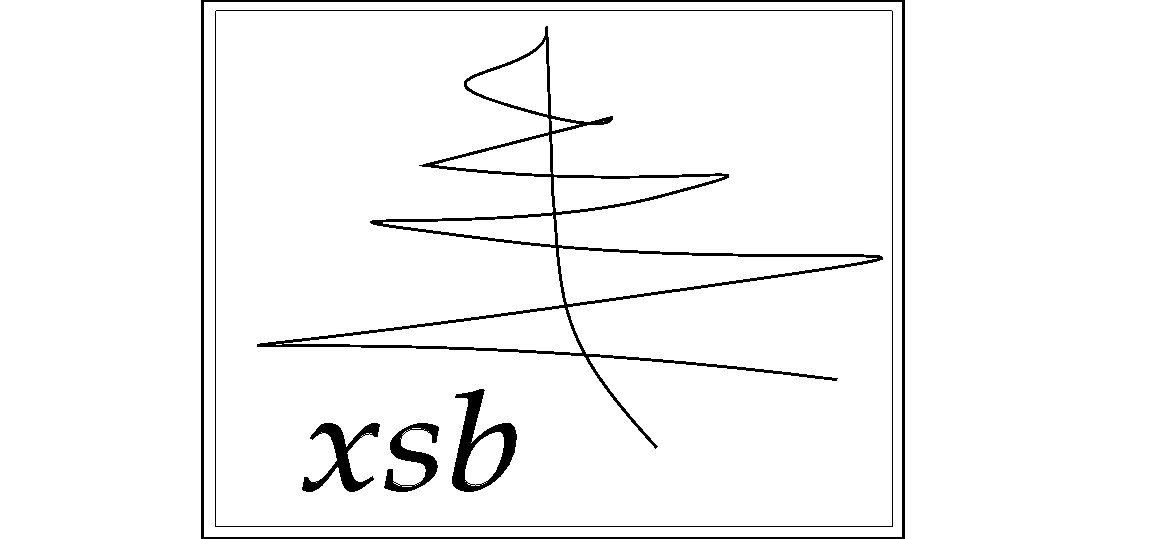
\includegraphics[width=2.5in]{xsb-logo}}\\
        \ \\ 
        {\em Theresa Swift} \ \ \ 
        {\em David S. Warren} \\ 
        \ \\
        {\em Konstantinos Sagonas} \\
        {\em Juliana Freire} \\
        {\em Prasad Rao} \\
        {\em Baoqiu Cui} \\
        {\em Ernie Johnson} \\
        {\em Luis de Castro} \\
        {\em Rui F. Marques} \\
        {\em Diptikalyan Saha} \\
        {\em Steve Dawson} \\
        {\em Michael Kifer} 
%        \ \\
}

\begin{document}

\thispagestyle{empty}
\maketitle

%\thispagestyle{empty}
\pagenumbering{roman}
\begin{center}
{\bf {\Large 
		Credits
            %=============%
}}
\end{center}

% Apologies to anyone I left out...  It wasn't intentional! TLS.

\begin{quote}
Day-to-day care and feeding of XSB including bug fixes, ports, and
configuration management is currently done by David Warren and
Theresa Swift with the help of Michael Kifer and others.  In the past
Kostis Sagonas, Prasad Rao, Steve Dawson, Juliana Freire, Ernie
Johnson, Baoqiu Cui, Bart Demoen and Luis F.  Castro have provided
tremendous help.

In \version, the core engine development of the SLG-WAM has been
mainly implemented by Theresa Swift, David Warren, Kostis Sagonas,
Prasad Rao, Juliana Freire, Ernie Johnson, Luis Castro and Rui
Marques.  The breakdown, very roughly, was that Theresa Swift wrote
the initial tabling engine, the SLG-WAM, and its built-ins; and leads
the current development of the tabling subsystem.  Prasad Rao
reimplemented the engine's tabling subsystem to use tries for
variant-based table access and Ernie Johnson extended and refactored
these routines in a number of ways, including adding call subsumption.
Kostis Sagonas implemented most of tabled negation.  Juliana Freire
revised the table scheduling mechanism starting from Version~1.5.0 to
create the batched and local scheduling that is currently used.
Baoqiu Cui revised the data structures used to maintain delay lists,
and added attributed variables to the engine.  Luis Castro rewrote the
emulator to use jump tables and wrote a heap-garbage collector for the
SLG-WAM.  Rui Marques was responsible for the concurrency control
algorithms used for shared tables, and mainly responsible for making
the XSB engine multi-threaded.  The incremental table maintenance
subsystem was designed and first implemented by Diptikalyan Saha, and
its design and development has been continued by Theresa Swift.
Answer subsumption was written by David Warren and Theresa Swift.
David Warren implemented hash-consed, or ``interned'' tables.  Call
abstraction and answer abstraction (restraint) were written by
Theresa Swift.

Other engine work includes the following.  Memory expansion code for
WAM stacks was written by Ernie Johnson, Bart Demoen and David
S. Warren.  Heap garbage collection was written by Luis de Castro,
Kostis Sagonas and Bart Demoen.  Atom space garbage collection was
written by David Warren; table garbage collection was written by
Theresa Swift based in part on space reclamation code written by
Prasad Rao.  Rui Marques rewrote much of the engine to make it
compliant with 64-bit architectures.  Assert and retract code was
based on code written by Jiyang Xu; it significantly revised by David
S. Warren, who added alternative, multiple, and star indexing and by
Theresa Swift who implemented dynamic clause garbage collection. Trie
assert/retract code, and trie interning code was written by Prasad
Rao.  Neng-fa Zhou, Theresa Swift and David Warren upgraded XSB from
ASCII to the character sets UTF-8, C1253, and LATIN-1.  The current
version of {\tt findall/3} was re-written from scratch by Bart Demoen,
as was XSB's original throw and catch mechanism.  64-bit floats were
added by Charles Rojo.  The interface from C to Prolog and DLL
interface were implemented by David Warren and extended to
multi-threading by Theresa Swift; the interface from Prolog to C
(foreign language interface) was developed by Jiyang Xu, Kostis
Sagonas, Steve Dawson and David Warren.

In terms of core system Prolog code, Kostis Sagonas was responsible
for HiLog compilation and associated built-ins as well as coding or
revising many standard predicates.  Steve Dawson implemented
Unification Factoring.  The revision of XSB's I/O into ISO-compatible
streams was done by Michael Kifer and Theresa Swift.  The {\tt
  auto\_table} and {\tt suppl\_table} directives were written by
Kostis Sagonas.  The DCG expansion module was written by Kostis
Sagonas for non-tabled code and by Baoqiu Cui, David Warren and
Theresa Swift for tabled code.  The handling of the {\tt multifile}
directive was written by Baoqiu Cui and David
Warren. C.R. Ramakrishnan wrote the mode analyzer for XSB.  Michael
Kifer implemented the {\tt storage} module.  The multi-threaded API
was written by Theresa Swift and Rui Marques.  Walter Wilson has
written several of XSB's library predicates for tabling.  Paulo Moura
has added several predicates to make XSB more consistent with other
Prologs.  

Michael Kifer has been in charge of XSB's installation procedures,
rewriting parts of the XSB code to make XSB configurable with GNU's
Autoconf, implementing XSB's package system, and integrated GPP with
XSB's compiler.  GPP, the source code preprocessor used by XSB, was
written by Denis Auroux, who also wrote the GPP manual reproduced in
Appendix A.

The starting point of XSB (in 1990) was PSB-Prolog 2.0 by Jiyang Xu
and David Warren.  PSB-Prolog in its turn was based on SB-Prolog,
primarily designed and written by Saumya Debray, David S. Warren, and
Jiyang Xu.  Thanks are also due to Weidong Chen for his work on Prolog
clause indexing for SB-Prolog, to Richard O'Keefe, who contributed the
Prolog code for the Prolog reader and the C code for the tokenizer, to
Ciao Prolog whose {\tt write\_term/[2,3]} we use, and to SWI Prolog
for their CLP(R) package.

... Now what did I forget this time ?

\end{quote}

%%% Local Variables: 
%%% mode: latex
%%% TeX-master: "manual1"
%%% End: 


%\newpage
\tableofcontents
\newpage        % Just to avoid a silly LaTeX bug with \pagenumbering
  
\pagenumbering{arabic}


\chapter{Introduction}

\begin{quote}
{\it  ``If logic programmers developed sushi, they'd market it as
cold dead fish''.} 
\end{quote}
\ \\

Logic programming in its various guises: using Prolog with logical
constraints, or using Answer Set Programming, can provide a useful
mechanism for representing knowledge, particularly when a program
requires default knowledge.  However formal ontologies based on
description logics have also received a great deal of attention as
formalisms for knowledge representation.  Description logics have a
clear semantics as a subset of first-order logic in which determining
consistency (and implication) of a set of sentences is decidable.
Furthermore, the worst-case complexity of these problems is
well-understood for various description logics.  From a practical
point of view, a user's intuitions about object-oriented programming
are helpful when ontologies are first encountered, since information
in ontologies consists of descriptions of classes, objects and
relations.  In addition, ontologies can be readily visualized and, in
certain cases, manipulated by non-programmers using grapical
interfaces (e.g.~\cite{protege}, and many others).  This has led to a
profusion of systems based around description logics
(see~\cite{MolH03} for a review of some of these systems), and to
standard representations that allow such systems to exchange
knowledge, such as the recent OWL standard~\cite{SMVW02}.

The {\em CDF} system allows various sorts of support for management of
formal ontologies from within XSB.  The full version of CDF is called
the {\em Coherent Description System} which has been developed largely
by XSB, Inc and has been heavily used in commercial software systems
that extract information from free text, gather information from the
world-wide web; and classify input strings according to given
ontologies.  Many of these applications generate code based on
information in an ontology, with the result that CDF has formed the
basis for model-driven commercial architectures.  An open-source
version of CDF is called {\em Cold Dead Fish} and contains many,
though not all, of the features of the Coherent Description System.
In this manual we describe all of CDF and note in passing which parts
of it are open-source and which proprietary.

A high-level architecture of CDF is shown in Figure~\ref{fig:arch}.
CDF stores knowledge in a {\em CDF Instance} consisting of information
in the form of Prolog facts (called extensional facts), Prolog rules
(called intensional rules), or in various database-resident formats.
Throughout the CDF architecture, information produced by evaluating
intensional CDF rules is handled in the same manner as that produced
by asserting extensional CDF facts.  This includes query evaluation,
consistency checking, update, and other routines.  CDF intensional
rules themselves are executed upon being invoked by a goal.  Thus when
intensional rules are written in Prolog they avoid the
view-maintenance problems that arise when forward-chaining rules are
updated; when tabling is used CDF provides predicates that allow
tables to be abolished whenever a CDF instance changes.  In addition,
the goal orientation of the rules allows CDF to lazily obtain
information from databases; and the various CDF database interfaces
allow maintenance of ontologies that are too large for the virtual
memory of a given machine.

%--------------
\begin{figure}[htbp] 
\centering {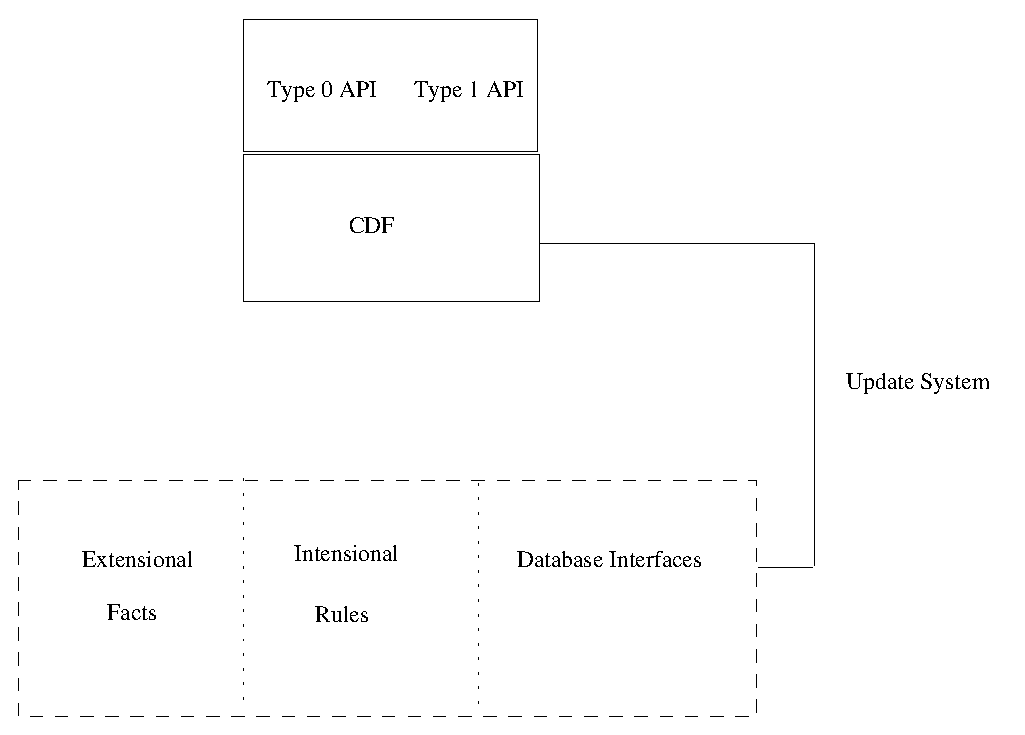
\epsfig{file=Figures/arch.eps,width=0.80\textwidth}}
\caption{A High-Level Architecture of CDF and XJ}
\label{fig:arch}
\end{figure}
%--------------

CDF instances can be classified either as Type-0 or a Type-1, each of
which has its own interface.  Type-0 instances are useful for storing
large amounts of information; and consistency and implication in
Type-0 instances is computable in polynomial time.  Type-0 instances
describe classes by existential and universal relations, qualified
number restrictions, and relational hierarchies, but descriptions omit
negation and disjunction. Type-0 instances also support a direct
product construction for objects and classes.  
\mycomment{
These product classes and objects can be useful for representing
certain types of non-binary relations, and are particularly useful for
incorporating knowledge represented as RDF facts \cite{}.  }
Information in Type-0 CDF instances is tightly coupled to XSB's
query mechanism, and CDF ensures that only the most specific answers
(according to a given inheritance hierarchy) are returned for any
Type-0 query.

Type-1 instances extend Type-0 instances to describe classes using
negation and disjunction, and thus permit descriptions that are
equivalent to an expressive description logic.  In fact, a Type-1 CDF
instance can be seen as a knowledge base in which various classes are
described via {\em class expressions}, which correspond to formulas in
description logics.  Reasoning in Type-1 instances is done via the CDF
theorem-prover.  Using the Type-1 API, users may ask whether a given
class or object is consistent, whether a given class expression is
consistent with a class or object; or whether a given class expression
is entailed by a given class or object.  The problems of determining
consistency or entailment of a Type-1 class expression have a high
degree of complexity.  To solve these problems the CDF theorem prover
uses several heuristics, but a determined (or unlucky) user can always
find class expressions that require a large amount of time to check.

Of course, ontology management systems require many features in
addition to reasoning and representation features \cite{MGPS03}.  We
mention some of these features.

\begin{itemize}
\item {\em A Semantic Checking System}.  CDF has various mechanisms for
ensuring consistency of objects and classes both at the Type-0 or
Type-1 level.  Various levels of consistency can be checked during
various operations on the CDF instance.
%
\item {\em A Component System}. Reusability of ontologies is supported
by the {\em component} structure of CDF.  An ontology component may be
maintained by separate users or organizations in different locations
and assembled in various ways by applications.
%
\item {\em A Concurrency System}. (Non open-source) Based on the
component structure, the {\em concurrency} mechanism for CDF allows
users to update their own CDF instances and to periodically update a
common store. Naturally, the various mechanisms in CDF for ensuring
consistency that are vital to ensuring coherency when users update
their systems concurrently.
%
\item {\em Database Interfaces}. (Non open-souce) CDF supports various
interfaces to databases so that CDF facts can be stored in a database
or mapped to database tables.
\end{itemize}

Based on these features, CDF can support user interfaces in a number
of ways.  One of the most convenient is to use a XSB/Java interface
such as InterProlog~\cite{Cale01} or JAXSB~(see
\texttt{http://xsb.sourceforge.net}) and then write a user interface in
Swing or some other Java Graphics library.  One of the easiest ways to
do this is to make use of the {\em XJ system} which allows Swing Gui
objects to be represented as Prolog terms (the XJ system is non
open-source) From a systems perspective, a graphical interface is then
written XJ library Swing widgets or specialized XJ-CDF Swing widgets.
CDF per-se has the following graphical packages and applications.
%
\begin{itemize}
%
\item {\em An XJ Caching System}. Adds and deletes to CDF are extended
with a notification mechanism so that Java Swing objects (created with
XJ, XSB's graphics system) reflect the state of CDF even when it
dynamically changes.
%
\item {\em A Visual Editor}. Finally,  CDF supports a graphical editor
that allows users both to visualize an ontology and to perform the
functions mentioned so far.
\end{itemize}
%
Extensional facts, intensional rules, updates, the Type-0 and Type-1
interfaces, consistency checking predicates and the full component
system are available as an open-source package for XSB.  Other
features, concurrency mechanisms, specialized database interfaces, XJ
support and the editor are not open-source.  The open-source code can
be obtained via \texttt{xsb.sourceforge.net}.  Inquiries about the full
Coherent Description System should be made to
\texttt{ode@xsb.com}.




\chapter{Getting Started with XSB} \label{quick_start}
%=====================================================

This section describes the steps needed to install XSB under UNIX and
under Windows.

\section{Installing XSB under UNIX}
%==================================
\label{installation_options}

If you are installing on a UNIX platform, the version of XSB that you
received may not include all the object code files so that an
installation will be necessary.  The easiest way to install XSB is to
use the following procedure.

\begin{enumerate}
\item	Decide in which directory in your file system you want to install
  XSB and copy or move XSB there.
\item Make sure that after you have obtained XSB, you have
  uncompressed it by following the instructions found in the file {\tt
    README}.
  
\item Note that after you uncompress and untar the XSB tar file, a
  subdirectory {\tt XSB} will be created in the current directory. All
  XSB files will be located in that subdirectory.  In the rest of this
  manual, we use {\tt \$XSB\_DIR} to refer to this subdirectory.  Note
  the original directory structure of XSB must be maintained, namely,
  the directory {\tt \$XSB\_DIR} should contain all the subdirectories
  and files that came with the distribution. In particular, the
  following directories are required for XSB to work: \verb'emu',
  \verb'syslib', \verb'cmplib', \verb'lib', \verb'packages',
  \verb'build', and \verb'etc'.

\index{configuration}
\index{installation into shared directories}
\item Change directory to {\tt \$XSB\_DIR/build} and then run these commands:
  %%
  \begin{quote}
    \tt
    configure\\
    \tt
    makexsb
  \end{quote}
  %%
  %%$
  This is it!
  
  In addition, it is now possible to install XSB in a shared directory
  ({\it e.g.}, {\tt /usr/local}) for everyone to use.  In this situation,
  you should use the following sequence of commands:
  %%
  \begin{quote}
    \tt
    configure --prefix=\$SHARED\_XSB\\
    \tt
    makexsb\\
    \tt
    makexsb install
  \end{quote}
  %%$
  where {\tt \$SHARED\_XSB}  denotes the shared directory where XSB is
  installed.  In all cases, XSB can be run using the script
  %%$
  \begin{quote}
    \tt
    \$XSB\_DIR/bin/xsb
  \end{quote}
  However, if XSB is installed in a central location, the script for
  general use is:
  \begin{quote}
    \verb'<central-installation-directory>/<xsb-version>/bin/xsb'
  \end{quote}
\end{enumerate}
  %%

{\bf Important:} The XSB executable determines the location of the
libraries it needs based on the full path name by which it was invoked.
The ``smart script'' \verb|bin/xsb| also uses its full path name to
determine the location of the various scripts that it needs in order to
figure out the configuration of your machine.  Therefore, there are certain
limitations on how XSB can be invoked.

Here are some legal ways to invoke XSB:
%%
\begin{enumerate}
\item  invoking the smart script \verb|bin/xsb| or the XSB executable using
  their absolute or relative path name.
\item using an alias for \verb|bin/xsb| or the executable.
\item creating a new shell script that invokes either \verb|bin/xsb| or the
  XSB executable using their {\em full\/} path names. 
\end{enumerate}
%%

Here are some ways that are guaranteed to not work in some or all cases:
%%
\begin{enumerate}
\item  creating a hard link to either \verb|bin/xsb| or the executable and
  using {\it it\/} to invoke XSB. (Symbolic links should be ok.)
\item changing the relative position of either \verb|bin/xsb| or the
  XSB executable with respect to the rest of the XSB directory tree.
\end{enumerate}
%%

The configuration script allows many different options to be
specified.  A full listing can be obtained by typing {\tt
\$XSB\_DIR/build/configure --help}.
%%
\begin{description}
\item[Type of Machine.]  The configuration script automatically
  detects your machine and OS type, and builds XSB accordingly. On
  64-bit platforms, the default compilation of XSB will reflect the
  default for the C compiler (e.g. gcc) on that platform.  Moreover,
  you can build XSB for different architectures while using the same
  tree and the same installation directory provided, of course, that
  these machines are sharing this directory, say using NFS or
  Samba. All you will have to do is to login to a different machine
  with a different architecture or OS type, and repeat the above
  sequence of commands -- or configure with different parameters.
  
  The configuration files for different architectures reside in
  different directories, and there is no danger of an architecture
  conflict.  In fact, you can keep using the same {\tt ./bin/xsb}
  script regardless of the architecture. It will detect your
  configuration and will use the right files for the right
  architecture!

  If XSB is being built on a Windows machine in which Cygwin
  is installed, Cygwin and Windows are treated as separate operating
  systems, as their APIs are completely different.  On such a machine, XSB
  can be built either for Cygwin or Windows.

\index{cc (compiler)} \index{gcc} \index{acc (compiler)}  
\item[Choice of the C Compiler and compiler-related
  options] \label{cc} On Unix systems, XSB is developed and tested
  mainly using gcc.  Accordingly, the {\tt configure} script will
  attempt to use {\tt gcc}, if it is available.  Otherwise, it will
  revert to {\tt cc} or {\tt acc}.  Some versions of {\tt gcc} are
  broken for particular platforms or {\tt gcc} may not have been
  installed; in which case you would have to give {\tt configure} an
  additional directive {\tt --with-cc} (or {\tt --with-acc}).  If you
  must use some special compiler, use {\tt
    --with-cc=your-own-compiler}.  You can also use the {\tt
    --with-optimization} option to change the default C compiler
  optimization level.  (or {\tt --disable-optimization} to disable all
  compiler optimizations).  {\tt --enable-debug} is mainly a
  development option that allows XSB to be debugged using gdb -- there
  are many other compiler-based options options.  Type {\tt configure
    --help} to see them all. Also see the file~\verb'$XSB_DIR/INSTALL'
  for more details.

\item[Word Size] XSB's configuration script checks whether the default
  compilation mode of a platform is 32- or 64-bits, and will build a
  version of XSB accoringly.  Some platforms, however, support both
  32-bit and 64-bit compilation.  On such a platform, a user can
  explicitly specify the type of compilation using the options {\tt
    with-bits32} and {\tt with-bits64}.  

\item[XSB and Site-specific Information] Using the option {\tt
  --prefix=PREFIX} installs architecture-independent files in the
  directory {\tt PREFIX}, e.g. {\tt /usr/local}, which can be useful
  if XSB is to be shared at a site.  Using the option {\tt
    --site-prefix=DIR} installs site-specific libraries in {\tt
    DIR/site}.  Other options indicate directories in which to search
  for site-specific static and dynamic libraries, and for include
  files.

%\item[Multi-threading] Version 3.0 of XSB was the first version that
%  supports multi-threading.  On some platforms, the multi-threaded
%  engine is slightly slower than the single-threaded engine, mostly
%  due to its need for concurrency control.  To obtain the benefits of
%  multiple threads on a platform that supports either POSIX or Windows
%  threads (i.e.  nearly all platforms) users must configure XSB with
 % the directive {\tt enable-mt} (see Section~\ref{sec:mt-windows} for
%  instructions specific to Windows. The multi-threaded engine works
%  with other configuration options, multi-threading can be compiled
%  with batched or local scheduling, with the ODBC or InterProlog
%  interfaces, and so on.

%%$
\index{InterProlog!Interface}
\index{Oracle Interface}
\index{SModels Interface}
\index{XASP}
\index{ODBC Interface}
\index{Tck/Tk}
\index{Interface!InterProlog}
\index{Interface!Oracle}
\index{Interface!SModels}
\index{XASP}
\index{Interface!ODBC}

\item[Interfaces] Certain interfaces must be designated at
configuration time, including those to Oracle, ODBC, Smodels, Tck/Tk,
and Libwww.  However, the XSB-calling-C interface interface does not
need to be specified at configuration time.  If you wish to use the
InterProlog Java interface that is based on JNI, you must
specify this at configuration time; otherwise if you wish to use the
sockets-based InterProlog interface, it does not need to be specified
at configuration time.  See Volume 2 and the InterProlog site {\tt
www.declarativa.com} for details of specific interfaces

While the XSB configuration mechanism can detect most include and
library paths, use of certain interfaces may require information about
particular directories.  In particular the {\tt
--with-static-libraries} option might be needed if compiling with
support for statically linked packages (such as Oracle) or if your
standard C libraries are in odd places. Alternately, dynamic libraries
on odd places may need to be specified at configuration time using the
{\tt --with-dynamic-libraries} option.  and finally, the {\tt
--with-includes} option might be needed if your standard header files
(or your {\tt jni.h} file) are in odd places, or if XSB is compiled
with ODBC support.  Type {\tt configure --help} for more details.

%%$
\index{scheduling strategy}
\item[Type of Scheduling Strategy.]  The ordering of operations within
a tabled evaluation can drastically affect its performance.  XSB
provides two scheduling strategies: Batched Evaluation and Local
Evaluation.  Local Evaluation ensures that, whenever possible,
subgoals are fully evaluated before there answers are returned, and
provides superior behavior for programs in which tabled negation is
used.  Batched Evaluation evaluates queries to reduce the time to the
first answer of a query.  Both evaluation methods can be useful for
different programs.  Since Version 2.4, Local Evaluation has been the
default evaluation method for XSB.  Batched Evaluation can be chosen
via the {\tt --enable-batched-scheduling} configure option.  Detailed
explanations of the scheduling strategies can be found in
\cite{JFLP-Scheduling}, and further experimentation in \cite{CaSW02}.

%
\end{description}

Other options are of interest to advanced users who wish to experiment
with XSB, or to use XSB for large-scale projects.  In general, however
users need not concern themselves with these options.

\subsection{Possible Installation Problems}


\paragraph*{Lack of Space for Optimized Compilation of C Code}
When making the optimized version of the emulator, the temporary space
available to the C compiler for intermediate files is sometimes not
sufficient. For example on one of our SPARCstations that had very
little {\tt /tmp} space the {\tt "-O4"} option could not be used for
the compilation of files {\tt emuloop.c}, and {\tt tries.c}, without
changing the default {\tt tmp} directory and increasing the swap
space.  Depending on your C compiler, the amount and nature of {\tt
/tmp} and swap space of your machine you may or may not encounter
problems.  If you are using the SUN C compiler, and have disk space in
one of your directories, say {\tt dir}, add the following option to
the entries of any files that cannot be compiled:

\demo{       -temp=dir}

\noindent
If you are using the GNU C compiler, consult its manual pages
to find out how you can change the default {\tt tmp} directory or how you
can use pipes to avoid the use of temporary space during compiling.
Usually changing the default directory can be done by declaring/modifying
the {\tt TMPDIR} environment variable as follows:

\demo{       setenv TMPDIR dir}

\paragraph*{Missing XSB Object Files}
When an object (*.xwam) file is missing from the {\tt lib} directories
you can normally run the {\tt make} command in that directory to
restore it (instructions for doing so are given in Chapter
\ref{quick_start}).  However, to restore an object file in the
directories {\tt syslib} and {\tt cmplib}, one needs to have a
separate Prolog compiler accessible (such as a separate copy of
XSB), because the XSB compiler uses most of the files in these
two directories and hence will not function when some of them are
missing.  For this reason, distributed versions normally include all
the object files in {\tt syslib} and {\tt cmplib}.

\paragraph*{XSB on 64-bit platforms}
\index{64-bit architectures}
%
XSB has been fully tested on 64-bit Debian Linux, 64-bit and Mac OS X.
However, the sockets library may have problems in \version{}.  If this
limitation prove a problem, please contact {\tt
  xsb-development@lists.sourceforge.net}~\footnote{64-bit XSB was
  broken in a recent releases prior to Version 3.1 because for a time
  the developers did not have access to a 64-bit machine.}.

Typically, if the 64-bit system generates 32-bit code by default, XSB
will run just as in 32-bit mode (including 64-bit floats).  64-bit
compilation can be forced for XSB by configuring with the option {\tt
  --with-bits64}, and in a similar manner 32-bit compilation can be
forced with the option {\tt --with-bits32}.  Users who employ either
option should be aware of issues that may arise when linking XSB to
external C code.  
\bi
\item When XSB calls C code the C file must have been compiled with
  the same memory option as XSB.  This is done automatically if the C
  file is compiled via a call from XSB's compiler, but must be handled
  by the user otherwise.  For instance, if XSB were configured {\tt
    --with-bits32} on a 64-bit machine defaulting to 64-bits, then C
  files called by XSB require the {\tt -m32} option in {\tt gcc} (if
  not compiled by XSB).
\item The appropriate memory option must be used when embedding XSB
  into a C or Java process.  For instance, if a XSB is to be linked
  into a 32-bit application on a 64-bit platform defaulting to
  64-bits, XSB must be configured {\tt --with-bits32}, and the linking
  of {\tt xsb.o/so} to the calling program must specify {\tt -m32}.
  \ei

\section{Installing XSB under Windows}
\subsection{Using Cygwin32 and Cygwin64}
\label{quick:cygwin}

This is easy: just follow the Unix instructions.
XSB can be built under CygWin64 or CygWin32, but in the latter case
CygWin32 must be installed on a 32 bit version of Windows.
XSB \emph{cannot} be built under CygWin32 if the latter is installed on a
64 bit Windows.

\noindent
\textbf{Note}: XSB is not fully functional under Cygwin---external C modules
cannot be linked and so several packages will not work.

\subsection{Using Microsoft Visual C++}
\label{quick:DOS}
%==========================================

\begin{enumerate}
\item Check XSB out from SVN:\\
  \texttt{svn checkout} \url{svn://svn.code.sf.net/p/xsb/src/trunk} \texttt{xsb-src}
\item Compile XSB as described below.
  This requires that Microsoft Visual Studio is installed.
\item After compiling XSB, it is OK to move it to some other place, if needed.
   However, make sure that the
   entire directory tree is moved --- the XSB executable looks for the files it
   needs relatively to its current position in the file system.
\end{enumerate}


The first thing is to ensure that
Microsoft Visual Studio that includes a C++ compiler, so
\emph{download the free of charge Microsoft Visual Studio, Community
    Edition} from
%% 
\begin{verbatim}
  https://www.visualstudio.com/vs/community/
\end{verbatim}
%% 
Make sure you \emph{select the C++ compiler}   as one of the additional components
to include (e.g., choose ``Desktop development with C++'').
The installer will place the studio in
\texttt{C:$\backslash$Program Files$\backslash$Microsoft Visual
  Studio$\backslash$}.

One way to compile XSB under Windows is to use the automatic installer:
%% 
\begin{quote}
\texttt{cd \$XSB\_DIR}   
\\
\texttt{java -jar InstallXSB.jar}
\end{quote}
%% 
where \texttt{\$XSB\_DIR} is the XSB's installation directory,
and follow the prompts. The trickiest of these prompts will ask you to provide the
full file name of the studio's settings batch file.
For Visual Studio 2017, Community Edition,
that file is \texttt{vcvarsx86\_amd64.bat} (for 64 bit apps) or
  \texttt{vcvars32.bat} (for 32 bit apps), located in the directory
  \vspace{1mm}\\
\texttt{
      C:$\backslash$Program Files\,(x86)$\backslash$Microsoft Visual Studio$\backslash$2017$\backslash$Community$\backslash$VC$\backslash$Auxiliary$\backslash$Build
    }
    \\
    In other versions of the studio, that file is elsewhere and can be
    found using the Windows search widget. For instance, in the 2015
    version of the studio, that directory is
\texttt{
      C:$\backslash$Program Files\,(x86)$\backslash$Microsoft Visual Studio 2015$\backslash$VC$\backslash$bin
    }

If the automatic method just described
does not work or if one needs customized installation,
one has to compile XSB the ``hard
way,'' as described below.

\begin{enumerate}
\item \emph{Find the settings file, which you need to execute in a command
  window in order to set the compilation environment}, as described above.
\item
    Open a Windows command prompt window and
    drag the appropriate batch file (\texttt{vcvarsx86\_amd64.bat} or
    \texttt{vcvars32.bat}) into it. Type \texttt{<Enter>} to execute that
    batch file. 
\item
   {\tt cd \$XSB\_DIR$\backslash$build}  
\item
To compile XSB as a 64 bit application, use the following command, where the
items in square brackets are optional and usually can be dropped:\\
  {\small{\tt makexsb64\,["CFG=opt"]\,["ORACLE=yes"]\,["MY\_LIBRARY\_DIRS=libs"]\,["MY\_INCLUDE\_DIRS=opts"]}}
  %%
  \begin{itemize}
  \item The options for {\tt CFG} are: \emph{release} (default) or \emph{debug}.  The
    latter is used when you want to compile XSB with debugging enabled.
  \item The {\tt ORACLE} parameter (default is ``no'') compiles XSB with
    native support for Oracle DBMS. If {\tt ORACLE} is
    specified, you {\bf must} also specify the necessary Oracle libraries
    using the parameter {\tt SITE\_LIBS}.
    Native Oracle support is rarely used and ODBC is the recommended way to
    connect to databases.
  \item \texttt{MY\_LIBRARY\_DIRS} is used to specify the external
    libraries and \texttt{libs} there has the form  \texttt{/LIBPATH:"libdir1"
    /LIBPATH:"libdir2" ...}.  
  \item \texttt{MY\_INCLUDE\_DIRS} is used to specify additional
    directories for included files. Here \texttt{opts} has the form
    \texttt{/I"incdir1" /I"incdir2" ...}.  
  \end{itemize}
  %%
  Instead of specifying the options on command line,
  it might be more convenient (and more general) to create the file
  %% 
\begin{verbatim}
  XSB\build\windows64\custom_settings.mak  
\end{verbatim}
  %% 
  and put the required options there. For instance,
  %% 
\begin{verbatim}
XSB_INTERPROLOG=yes 
MY_INCLUDE_DIRS=/I"C:\Program Files\Java\jdk1.8.0_131\include" \
      /I"C:\Program Files\Java\jdk1.8.0_131\include\win32" 
MY_LIBRARY_DIRS=/LIBPATH:"C:\pthreads\pthreadVC1.lib" /libpath:"C:\oracle"
ORACLE=yes
\end{verbatim}
  %% 
Make sure you do not misspell the name of that file or else none of the
specified options will take effect!
   
 \item The above command will compile XSB as requested and will put the XSB 
   executable and its DLL in:
%%
\[
\begin{array}{l}
 \tt
 \$XSB\_DIR\backslash{}config\backslash\texttt{x64-pc-windows}\backslash{}bin\backslash{}xsb.exe
\\
 \tt
 \$XSB\_DIR\backslash{}config\backslash\texttt{x64-pc-windows}\backslash{}bin\backslash{}xsb.dll
 \end{array}
\]

\item To compile XSB as a 32 bit application (\textbf{not} recommended),
  use \texttt{makexsb} instead of
  \texttt{makexsb64}. The compiled code will be installed   in
  %%
\[
\begin{array}{l}
 \tt
 \$XSB\_DIR\backslash{}config\backslash\texttt{x86-pc-windows}\backslash{}bin\backslash{}xsb.exe
\\
 \tt
 \$XSB\_DIR\backslash{}config\backslash\texttt{x86-pc-windows}\backslash{}bin\backslash{}xsb.dll
 \end{array}
\]
%%
\end{enumerate}
%%
The \texttt{custom\_settings.mak} file must then be in
%% 
\begin{verbatim}
  XSB\build\windows\custom_settings.mak  
\end{verbatim}
%% 

\noindent
{\bf Note}: if you compiled XSB with one set of parameters and then want to
recompile with a different set, it is recommended that you run
%%
\begin{verbatim}
 makexsb64  clean  
\end{verbatim}
%%
in between the compilations (or \texttt{makexsb clean} in the 32-bit
case).  
This also applies to recompilations for 64/32 bits.


\section{Invoking XSB}
%=====================

Under Unix, XSB can be invoked by the command:
\begin{quote}
       \tt \$XSB\_DIR/bin/xsb
\end{quote}
%%$
if you have installed XSB in your private directory.  If XSB is
installed in a shared directory ({\it e.g.}, {\tt \$SHARED\_XSB} for
the entire site (UNIX only), then you should use
\begin{quote}
       \tt \$SHARED\_XSB/bin/xsb
\end{quote}
%%
In both cases, you will find yourself in the top level interpreter.  
As mentioned above, this script automatically detects the system
configuration you are running on and will use the right files and
executables. (Of course, XSB should have been built for that architecture
earlier.)

Under Windows, you should invoke XSB by typing:
\[
 \tt
 \$XSB\_DIR\backslash{}bin\backslash{}xsb
\]
This script tries to find the XSB executable and invoke it. If, for some
reason, it fails to do so, the user should call the executable directly.
\[
 \tt
 \$XSB\_DIR\backslash{}config\backslash\texttt{x86-pc-windows}\backslash{}bin\backslash{}xsb.exe
\]
%%


You may want to make an alias such as {\tt \smallourprolog} to the above
commands, for convenience, or you might want to put the directory where the
XSB command is found in the {\tt \$PATH} environment variable. However, you
should {\bf not} make hard links to this script or to the XSB executable.
If you invoke XSB via such a hard link, XSB will likely be confused and will
not find its libraries.  That said, you {\bf can} create other scripts and
call the above script from there.

ISO``standard'' Prolog predicates are supported by XSB, in addition to
many other predicates: so those of you who consider yourselves
champion entomologists, can try to test them for bugs now.  Details
are in Chapter~\ref{standard}.


\section{Compiling XSB programs}
%===============================

One way to compile a program from a file, such as {\tt myfile.P} in
the current directory and load it into memory, is to type the query:
\begin{verbatim}
     [my_file].
\end{verbatim}
where \verb'my_file' is the name of the file.
Chapter~\ref{chap:system} contains a full discussion of the compiling
and consulting.

If you are eccentric (or you don't know how to use an editor) you can also 
compile and load predicates input directly from the terminal by using the
command:
\begin{verbatim}
     [user].
\end{verbatim}
A {\tt CTRL-d} or the atom \verb'end_of_file' followed by a period 
terminates the input stream.


\section{Sample XSB Programs}
%============================

There are several sample XSB source programs in the directory: {\tt
  \$XSB\_DIR/examples} illustrating a number of standard features, as
well as a number of non-standardized or XSB-specific features
including plain tabling, incremental tabling, tabling with negation,
attributed variables, annotated programs, constraint handling rules,
XSB embedded in a C program, XSB calling C functions, sockets, and
various semantic web application

Hence, a sample session might look like
(the actual times shown below may vary and some extra information is given
using comments after the \% character):

{\footnotesize
 \begin{verbatim}
my_favorite_prompt> cd $XSB_DIR/examples
my_favorite_prompt> $XSB_DIR/bin/xsb
XSB Version 3.1 (Incognito) of August 10, 2007
[i386-apple-darwin8.9.1; mode: optimal; engine: slg-wam; scheduling: local; word size: 32]
| ?- [queens].
[queens loaded]

yes
| ?- demo.

% ...... output from queens program .......

Time used: 0.4810 sec

yes
| ?- statistics.

memory (total)         1906488 bytes:       203452 in use,      1703036 free
  permanent space       202552 bytes
  glob/loc space        786432 bytes:          432 in use,       786000 free
    global                                     240 bytes
    local                                      192 bytes
  trail/cp space        786432 bytes:          468 in use,       785964 free
    trail                                      132 bytes
    choice point                               336 bytes
  SLG subgoal space          0 bytes:            0 in use,            0 free
  SLG unific. space      65536 bytes:            0 in use,        65536 free
  SLG completion         65536 bytes:            0 in use,        65536 free
  SLG trie space             0 bytes:            0 in use,            0 free
   (call+ret. trie           0 bytes,     trie hash tables            0 bytes)

      0 subgoals currently in tables
      0 subgoal check/insert attempts inserted     0 subgoals in the tables
      0 answer  check/insert attempts inserted     0 answers  in the tables

       Time: 0.610 sec. cputime,  18.048 sec. elapsetime

yes
| ?- halt.          % I had enough !!!

End XSB (cputime 1.19 secs, elapsetime 270.25 secs)
my_favorite_prompt>
 \end{verbatim}
}


\section{Exiting XSB}
%====================

If you want to exit XSB, issue the command \verb'halt.' or
simply type \verb'CTRL-d' at the XSB prompt. To exit XSB while it is
executing queries, strike \verb'CTRL-c' a number of times.


%%% Local Variables: 
%%% mode: latex
%%% TeX-master: "manual1"
%%% End: 

\chapter{System Description} \label{chap:system}
\label{system}

Throughout this chapter, we use \verb'$XSB_DIR' to refer to the
directory in which XSB was installed.

\section{Entering and Exiting XSB from the Command Line}
%=================================

After the system has been installed, the emulator's executable code appears 
in the file:
\begin{verbatim}
                     $XSB_DIR/bin/xsb
\end{verbatim}
If, after being built, XSB is later installed  at a central location,
\verb'$SHARED_XSB', the emulators executable code appears in
\begin{verbatim}
                     $SHARED_XSB/bin/xsb
\end{verbatim}
Either of these commands invokes XSB's top-level interpreter, which is
the most common way of using XSB.

XSB can also directly execute object code files from the command line
interface.  Suppose you have a top-level routine {\tt go} in a file
{\tt foo.P} that you would like to run from the UNIX or Windows
command line.  As long as {\tt foo.P} contains a directive, e.g. {\tt
  :- go.}, and {\tt foo.P} has been compiled to an object file ({\tt
  foo.xwam}), then
\begin{verbatim}
                     $XSB_DIR/bin/xsb foo
\end{verbatim}
will execute {\tt go} (and any other directives), loading the
appropriate files as needed~\footnote{In XSB, all extensions except
  '.pl' and '.prolog' --- (default '.P', '.H', '.xwam', '.D' (output by mode
  inferencing), and '.A' (assembly dump) --- are defined in C and
  Prolog code using macros in {\tt \$XSB\_DIR/emu/extensions\_xsb.h}
  and can be changed by a user if desired.  Of course, such a step
  should not be taken lightly, as it can cause severe compatibility
  problems.}.
%
In fact the command
\verb'$XSB_DIR/bin/xsb' is equivalent to the command:
\begin{verbatim}
             $XSB_DIR/bin/xsb -B $XSB_DIR/syslib/loader.xwam
\end{verbatim}
%%$
There is one other way to execute XSB from a command line.  Using the
{\tt -e} command-line option any goal can be can be executed, up to
1024 characters.  For instance 
\begin{verbatim}
             $XSB_DIR/bin/xsb -e "writeln('hello world'),halt."
\end{verbatim}
%%$
writes ``hello world'' and exits XSB.  Within the 1024 character
limit, any query or command can be executed, including consulting
files, so this method is actually quite general~footnote{Various
  options can suppress XSB's startup and end messages, as discussed
  below.}.

There are several ways to exit XSB.  A user may issue the
command \verb'halt.' or \verb'end_of_file.', or simply type
\verb'CTRL-d' at the XSB prompt.  To interrupt XSB
while it is executing a query, strike \verb'CTRL-c'.

\section{The System and its Directories}
%=======================================
When installed, the XSB system resides in a single directory that
contains several subdirectories.  For completeness, we review the
information in all subdirectories.  Normally, only the documentation
and files in the Prolog subdirectories, particularly {\tt examples},
{\tt lib}, and {\tt packages} will be of interest to users.
\begin{enumerate}
\item {\tt bin} contains scripts that call XSB executables
for various configurations.
%
\item {\tt build} contains XSB configuration scripts.  You may
already be familiar with the {\tt build} directory, which is used to
build XSB.
%
\item {\tt config} contains executables and other files specific to
particular configurations.
%
\item {\tt docs} contains the user manuals and other documentation,
including homepage sources.  
%
\item {\tt emu} contains the C source code for the XSB virtual
  machine, for I/O and for various interfaces.
%
\item {\tt etc} contains miscellaneous files used by XSB.
%
\item {\tt examples} contains some examples for Prolog, tabling,
HiLog and various interfaces.
%
\item {\tt cmplib} contains Prolog source and object code for the
compiler. 
%
\item {\tt gpp} contains a copy of the Gnu pre-processor used to
  preprocess Prolog files when they are compiled or dynamically
  loaded (i.e., loaded as dynamic code).
%
\item {\tt lib} contains Prolog source and object code for extended
librarie (cf. Section~\ref{library_utilities}). 
%
\item {\tt packages} The directory {\tt packages} contains various
  interfaces (e.g., {\tt sgml}, {\tt minizinc}, {\tt curl} and {\tt
    dbdrivers}); applications, such as {\tt chr}, {\tt pita} and {\tt
    cdf}. along with a number of other interfaces and applications.
  These packages are described in Volume 2 of this manual.
%
\item {\tt Prolog\_includes} contains include files for the Prolog
libraries, which are preprocessed using GPP.
%
\item {\tt syslib} contains Prolog source and object code for core XSB
libraries. 
\end{enumerate}

\noindent
All Prolog source programs are written in XSB, and all object (byte
code) files contain SLG-WAM instructions that can be executed by the
virtual machine.  These byte-coded instructions are
machine-independent, so usually no installation procedure is needed
for the byte code files.

If you are distributing an application based on XSB and need to cut
down space, the {\tt packages}, {\tt examples} and {\tt docs}
directories are not usually needed (unless of course you are using one
of the packages in your application).  {\tt lib} might not be needed,
(most core system files are in syslib) nor are Prolog source files
necessary if they have already been compiled into byte code.  Unless
your application needs to rebuild XSB, the {\tt emu} and {\tt build}
directories do not need to be distributed.

\section{How XSB Finds Files: Source File Designators}  \label{sec:filenames}
%
\index{base file name}
\index{source file designator}
Three files are associated with Prolog source code in
XSB~\footnote{Other types of files may be associated with foreign code
--- see Volume 2.}.
\begin{itemize}
\item A single {\it source} file, whose name is the {\em base file
  name} plus an optional extension suffix {\tt .P}, {\tt .pl}, or {\tt .prolog}.
\item An {\it object (byte-code)} file, whose name consists of the
  base file name plus the suffix {\tt .xwam}.
\item An optional {\it header} file, whose name is the base file name
  plus the suffix ``{\tt .H}''.  When used, the header file normally
  contains file-level declarations and directives while the source
  file usually contains the actual definitions of the predicates
  defined in that module.  However, such information can be
  equivalently put into the {\tt .P} ({\tt .pl}, or {\tt .prolog}) file.
\end{itemize}
%
Most of the XSB system predicates for compiling, consulting, and
loading code, such as {\tt consult/[1,2]}, {\tt compile/[1,2]}, {\tt
  load\_dyn\_gen/2} and others are somewhat flexible in how they
designate the file of interest.  Each of these predicates take as
input a {\em source file designator} which can be a base file name, a
source file name; or the relative or absolute paths to a base or
source file name.  Unfortunately, in \version{} there remain minor
differences in the ways in which the file designator can be indicated,
by different system predicates across different platforms.

In general, however, when given a source file designator, system
predicates perform {\em name resolution}.  There are two steps to name
resolution: determining the proper directory prefix and determining
the proper file extension.  When {\tt FileName} is absolute (i.e. it
contains a path from the file to the root of the file system)
determining the proper directory prefix is straightforward.  If {\tt
  FileName} is relative, i.e. it contains a {\tt '/'} in Unix or
\verb|\| in Windows, {\tt FileName} is expanded to a directory prefix
in an OS-dependent way, resolving symbols like {\tt '.'}, {\tt '..'}
and {\tt '\~{}'} when applicable.  However, the user may also enter a
name without any directory prefix. In this case, XSB tries to
determine the directory prefix using a set of directories it knows
about: those directories in the on-demand loader path (see
Section~\ref{LibPath}).  As it searches through directory prefixes,
different forms of the file name may be checked.  If the source file
designator has no extension the loader first checks for a file in the
directory with the {\tt .P} extension, (or {\tt .c} for foreign
modules); next checks for a file without the extension; and finally
checks for a file with a {\tt .pl} or {\tt .prolog} extension.  Note
that since directories in the on-demand loader path are searched in a
predetermined order (see Section~\ref{LibPath}), if the same file name
appears in more than one of these directories, the first one
encountered will be used.

% attempt to re-document the XSB module system

\index{modules}
\section{The Module System of XSB} \label{Modules}

XSB has been designed as a module-oriented Prolog system.  Modules
provide a step towards {\em logic programming ``in the large''} that
facilitates the construction of large programs or projects from
components that are developed, compiled and tested separately.  Also,
module systems support the principle of information hiding and can
provide a basis for data abstraction.  And modules form the basis for
XSB's implementation of its standard predicates, and for the on-demand
loading of standard and user predicates.

The module system of XSB is {\em file based} -- one module per file --
and {\em flat} -- modules cannot be nested.  In addition, XSB's module
system is essentially {\em structure-symbol-based}, where any compound
symbol in a module can be imported, exported or be a local symbol, as
opposed to a {\em predicate-based} one where this can be done only for
predicate symbols.~\footnote{Operator symbols can be exported as any
  other symbols, but their precedence must be redeclared in the
  importing module.}  In XSB, every structure symbol (and thus
structured term) is associated with a module, and structure symbols
with the same name but in different modules are different symbols and
thus do not unify.  On the other hand, XSB does not require a
meta-predicate to be explicitly declared as such in order to be used
in a module.  As we will discuss, these differences lead to certain
incompatibilities with the predicate-based module systems supported by
most other Prologs.  Although the differences are important, XSB's
module system is quite often compatible with those of other Prologs:
for instance, XSB's module system is able to support the Prolog
Commons libraries.

In Prolog systems a predicate definition (aka a set of rules) may be
associated with a structure symbol.  In other words, a predicate
symbol is just a structure symbol with an associated definition.
Accordingly, predicates are either static or dynamic depending on how
they are defined.  Static predicates get their definitions from source
code files that are compiled and loaded into memory.
The definition of a static predicate cannot be changed by adding ar
deleting clauses using {\tt assert/1} or {\tt retract}, or similar
predicates.
A dynamic
predicate $P$ may also occur in a compiled source file if there is a
dynamic declaration for $P$, of if $P$ is in a file that is loaded as
dynamic code via {\tt load\_dyn/[1,3]} or similar predicates.  $P$ is
also dynamic if rules for $P$ have been asserted to the Prolog data
store.  Dynamic predicates can have their definitions changed by {\tt
  assert/1} and {\tt retract/1}.

In XSB every structure symbol is associated with a module -- not just
predicates.  A term is said to be in the module of its main structure
symbol.  Terms in different modules are different terms and do {\bf
  not} unify.  So two terms whose main structure symbols (or any
structure symbols) have the same name but different modules, are
different terms and do not unify.  So, for example, terms printed as
{\tt p(a,b)} and {\tt p(a,b)} would not unify if the first structure
symbol named {\tt p/2} is in a different module from the second
structure symbol named {\tt p/2}. \footnote{This lack of unification
  also occurs in most other Prologs if the structure symbols are
  predicate symbols that occur in other modules.}

\index{modules!declaration}
So how are terms in a module created?  The most common way
is for a term to occur in a Prolog source file $F_{mod}.P$ that contains
a {\em module declaration} such as

\demo{:- export $Pred/Arity$.}

or

\demo{:- module($F_{mod}$,[$Pred/Arity$]).}

\index{modules!qualification}
\noindent 
where $F_{mod}$ is compiled as static code and loaded into a session,
or loaded as dynamic code into a session.  In either case, the name of
the module is the name of $F_{mod}$, the file name without its extension.
In addition, a file $F_{nomod}.P$ can be loaded into a module as dynamic
code via the appropriate option in {\tt load\_dyn\_gen/2} and similar
predicates.  Finally, a dynamic clause for a predicate $P$ can be
explicitly asserted into a module $M$ using the {\em module
  qualification} syntax for predicates, $M:P$.  For instance, via a
goal like

\demo{assert(M:P)}

\noindent
a rule can be asserted for $P$ in module $M$.  More generally, the
module qualification $M:P$ also causes P to be treated as belonging to
$M$ if $M:P$ occurs as a goal in any source file or input stream.

\index{modules!usermod}
\index{modules!declaration}

A predicate or goal $Pred$ is considered to be in the ``default''
module {\tt usermod} if none of the above situations occur,  i.e., if
$Pred$ does not have a module qualification, does not occur in a file
with a module declaration, and is not loaded into a module as dynamic
code.  Thus a term that has no module qualification when read from an
input stream is put into {\tt usermod}.  In addition, if a term is
created via {\tt functor/3} or {\tt =../2} it is also considered to be
in usermod.

Given a predicate $P$ in a module $M$, $P$ is usually accessed by
exporting it from $M$ and importing it to {\tt usermod} or some other
module via an import directive, such as:

\demo{:- import $Pred/Arity$ from $Module$.}

or

\demo{:- use\_module(Module,$Pred/Arity$).}

\noindent
For example, the file:
\begin{verbatim}
%% file: mod1.P
:- export p/2.

p(a,b).
p(X,Y) :- q(X,Y).

q(b,c).
\end{verbatim}
defines predicates {\tt p/2} and {\tt q/2} in {\tt mod1}.
%(i.e., {\tt p/2} terms
%that define the facts have their main structure symbols put in module
%{\tt mod1}, and the code implementing those clauses are associated
%with that structure symbol in that module.)  It also defines a
%predicate {\tt q/2} in the same module.  (And, of course, the call to
%{\tt q(X,Y)} in the body of the rule for {\tt p/2} is also put in that
%same module.)  The predicate {\tt p/2} is exported and is thus
%available for use by other code.
%
Continuing, we can create another file (not a module in this case),
which uses the definition of {\tt p/2} above:
\begin{verbatim}
%% file: my_code.P
:- import p/2 from mod1.

q(X,Y) :- p(X,Y).
\end{verbatim}
\noindent Here there is no {\tt export} directive, so all definitions
in this file will go into module {\tt usermod}.  The clause here
defines {\tt q/2} in {\tt usermod}, which is a different predicate
from the {\tt q/2} defined above in the module {\tt mod1}.  The {\tt
  import} of {\tt p/2} in this file causes the {\tt p(X,Y)} term in
the body of the rule for {\tt q/2} to be interpreted as being in
module {\tt mod1}.  Thus, {\tt my\_code} is compiled and loaded, {\tt
  q/2} is defined in {\tt usermod} and its code calls {\tt p/2} in
module {\tt mod1}.  Alternately, one could accomplish the same
functionality via:
\begin{verbatim}
%% file: my_other_code.P

q(X,Y) :- mod1:p(X,Y).
\end{verbatim}

A module source file may want to access a predicate defined in {\tt
  usermod}, which can be done by explicitly importing the predicate
from {\tt usermod}, or using {\tt usermod} as part of a module
qualification.

%There are situations in which a programmer wants to explicitly provide
%a module name to ``override'' the module associated with a term.  For
%example, one might want to call the goal {\tt p(X,Y)} to invoke the
%code associated with {\tt p/2} in module {\tt mod1} at the top level,
%%regardless of what module the {\tt p/2} structure symol is associated
%with.  In this case, one can write:
%
%\demo{| ?- call(mod1:p(X,Y)).}
%
%\noindent Here {\tt call} will construct the term {\tt p(X,Y)} with
%structure {\tt p/2} in module {\tt mod1} (ignoring the module associated
%with the {\tt p/2} structure symbol) and then call that term, which
%accesses the code of {\tt p/2} in module {\tt mod1}.  In this
%particular case the original term {\tt mod1:p(X,Y)} had the {\tt p/2}
%structure in {\tt usermod}, since that's where the top-level read puts
%it.  But {\tt call/1} interprets this term (with main structure symbol
%{\tt :/2}) as a coercion of the term {\tt p(X,Y)} into the module {\tt
%  mod1}.  In XSB, in most contexts in which a term is interpreted as a
%goal, the syntax of {\tt Mod:Goal} is interpreted as a coercion of
%term {\tt Goal} into the module {\tt Mod}.  And in fact, the top-level
%goal:
%
%\demo{| ?- mod1:p(X,Y).}
%
%\noindent is equivalent to the goal above.
%
%And instead of:
%\begin{verbatim}
%:- import pr/2 from mod3.
%...
%q(X,Y) :- ... pr(X,Z), ....
%\end{verbatim}
%one can directly write:
%\begin{verbatim}
%q(X,Y) :- ... mod3:pr(X,Z), ....
%\end{verbatim}

%In general, the use of {\tt import} is recommended, even though it may
%sometimes be more verbose.  The use of {\tt imort} allows for better
%visibility and easier analysis of module dependencies.

Returning to the topic of module declarations, in XSB the declaration:

\demo{:- module($filename$,[$sym_1$, \ldots, $sym_l$.]).}

\noindent
is syntactic sugar for:

\demo{:- export $sym_1$, \ldots, $sym_l$. }

\noindent
as long as the $filename$ is the same as the name of the file in which
it was contained.  Similarly,

\demo{:- use\_module($module$,[$sym_1$, \ldots, $sym_l$.]).}

\noindent
is treated as semantically equivalent to 

\demo{:- import $sym_1$, \ldots, $sym_n$ from $module$. }

\noindent
Accordingly, {\tt use\_module/2} and {\tt module/1} can be used
interchangeably with {\tt import/2} and {\tt export/1}.  However the
declaration

\demo{:- use\_module($module$).}

\noindent
which is often used in other Prolog systems, is {\em not} equivalent
to an XSB import statement, as each XSB import statement must
explicitly declare a list of predicates that are used from each
module.  Such a declaration will raise a compilation error. The main
reason for this is that the compiler needs to associate a module with
each structured term and this is facilitated by listing the imported
predicates explicitly.  In addition, including specific predicates in
an import statement facilitates the loading of modules on demand.

Finally, the declaration 

\demo{:- import $sym/n$ from $module$ as $sym'/n$. }

\noindent
allows a predicate to be imported from a module, but renamed as
$sym'/n$ within the importing module.  In this case the structure
symbol $sym'/n$ is placed in the current module and its code pointer
is identified with that of the structure symbol $sym/n$ in module
$module$.  Such a feature is useful when porting a library written for
another Prolog (e.g. a constraint library) to XSB.  As shown in the
next section, is also useful when one wants to import two predicates
with the same name from different modules.  In that case (at least)
one of the names needs to be changed on import.

For modules, the base file name is stored in its byte-code ({\tt
  .xwam}) file, so that renaming a byte-code file for a module may cause
problems, as the renaming will not affect the information within the
byte-code file.  (But see below for ways to support modules with
names different from the files that contain their code.)
However, byte-code files generated for non-modules
can be safely renamed.

\subsection{How the Compiler Determines the Module of a Term}

When XSB compiles a source code file, it must determine the module for
every term it encounters.  For non-module source files (i.e., those
lacking a module declaration), all terms are associated with {\tt
  usermod} except for those whose structure symbols are imported.  Any
occurrence of an imported structure symbol is associated with the
module from which it is imported.

For a module source code file $M$, i.e., where $M$ contains at least
one module declaration, the process of determining the module of a
structure symbol $t/n$ is more complicated.  The idea is that all
terms in $M$ that refer to predicates are placed in the module of the
file and all terms that are non-predicate structures are by default
placed in {\tt usermod}.  All occurrences of $T/N$ in $M$ are in a
file are normally associated with the same module.~\footnote{but see
  {\tt import .. as ..}  for an exception.}  So if $T/N$ appears both
as a predicate symbol and as a non-predicate structure (e.g., as an
argument in a body literal, both occurrences will be associated with
the current module.  Of course, imported structure symbols are
associated with the module from which they are imported.

The compiler recognizes as predicate symbols any symbol that:
\begin{enumerate}
\item appears as the main structure symbol in the head of a rule,

\item appears as a subgoal in the body of a rule,

\item appears as the main structure symbol of terms passed to known
  meta-predicates.  In \version{} these are listed in
  Table~\ref{tab:meta-predicates}.

\item is declared as {\tt dynamic}.
\end{enumerate}

\begin{table}[tbp]\centering{\tt
\begin{tabular}{lll}
abolish/2       & abolish\_table\_subgoals/[1,2] & abolish\_table\_subgoal/[1,2] \\
assert/1        & asserta/1                    & assertz/1\\
bagof/3         & call/[1-10]                  & call\_tv/1 \\ 
call\_cleanup/2 & catch/3                      & clause/2 \\ 
fail\_if/1      & findall/[3,4]                & forall/2 \\ 
not/1           & once/1                       & retract/1 \\ 
retractall/1    & setof/3                      & table\_once/1 \\ 
time/1          & tnot/1                       & \verb|\+|/1 \\ 
\verb|;|/2      & \verb|/|/2                   & \verb|->| /2   \\ 
do\_all/[1,2]   &                              &
\end{tabular}}
\caption{Meta-predicates known to XSB's Compiler}\label{tab:meta-predicates}
\end{table}

Otherwise a structure symbol is associated with {\tt usermod}.

Note that these rules imply that all structure symbols used solely as
non-predicate structures are placed by default in {\tt usermod}.  This
is usually what a user wants.  But there are times a user might want a
non-predicate structure to be associated with the current module --
for instance if a meta predicate is not among those listed in
Table~\ref{tab:meta-predicates}.  The programmer can tell the
compiler to place a particular structure symbol in the current module
by using the {\tt local} directive:

\demo{:- local $Sym/Arity$.}

\noindent which will force all uses of the indicated structure symbol
to be associated with the current module. \footnote{The low-level
  builtin {\tt term\_new\_mod/3} can be used to explicitly coerce a
  term into an arbitrary module, without using module qualification.}

%Associating a non-predicate
%structure with the module in which it appears also can be used to
%provide a measure of information hiding: Since no other module (or
%usermod) will construct a term associated with this module, another
%module can't use unification to look at the subfields inside such a
%term.  So in this way, a module can return to a caller a complex term,
%and the caller can pass it around and back to the module in a later
%call, and only the module code can manipulate thatq data
%structure.\footnote{The hiding is only partial, since other code can 
% use {\tt functor/3} or {\tt univ/2} to look inside such terms.  Also
%  the very low-level builtin {\tt term\_new\_mod/3} can be used to
%  explicitly coerce a term into an arbitrary module.}

An XSB programmer can also export a structure symbol (that is not used
as a predicate), and others can import and use it as a structure
symbol.

Standard predicates (those defined in the XSB environment) are
actually defined in system modules and the compiler implicitly
provides the necessary imports to allow the programmer to use them.
Standard predicates are described in Section \ref{sec:standard}.

For clarity, we state a few consequences of the above discussion.
\begin{itemize}
\item The module for a particular symbol appearing in a module must be
  uniquely determined.  As a consequence, a symbol of a specific
  $functor/arity$ generally cannot be declared as both exported and
  local, or both exported and imported from another module or declared
  to be imported from more than one module, etc.  Such environment
  conflicts are detected at compile-time and abort the compilation.
  One exception is the {\tt import ... as ...} directive.  Using this
  directive, one can import $symbol_1$ from a module {\tt as}
  $symbol_2$ and then export $symbol_2$.  (In fact, $symbol_1$ and
  $symbol_2$ are allowed to be the same symbol.)
%
\item If the {\tt import ... as ...} declaration is not used, a module
  {\em cannot} export a predicate symbol that is directly imported
  from another module, since this would require that symbol to be in
  two modules.
%
% Perhaps discuss symbols, if that isn't too confusing.
\index{Prolog flags!{\tt unknown}}
\item If a module {\tt m1} imports a predicate {\tt p/n} from a module
  {\tt m2}, but {\tt m2} does not export {\tt p/n}, nothing is
  detected at the time of compilation.  If {\tt p/n} is defined in
  {\tt m2}, a runtime warning about an environment conflict will be
  issued.  However, if {\tt p/n} is not defined in {\tt m2}, a runtime
  existence error will be thrown~\footnote{This behavior can be
    altered through the Prolog flag {\tt unknown}.}.
\end{itemize}

\subsection{Atoms and 0-Ary Structure Symbols}

XSB uses different internal representations for {\bf atoms} (i.e.,
constant functions) and for {\bf 0-ary structure
  symbols}. \footnote{Prolog terminology denotes non-numeric constants
  as atoms, which conflicts with the definition of an atomic term in
  mathematical logic.}  Atoms cannot have definitions associated with
them (i.e., cannot be predicates) and are not associated with modules.
But 0-ary predicates can and are.

In order to reduce ambiguity, a 0-ary predicate $p/0$ can be
designated as $p()$, in addition to $p$.

XSB automatically coerces atoms to 0-ary structure symbols and vice
versa in a manner analogous to the coercion for non-predicate
structures.
%But when coercing an atom to a 0-ary structure symbol, it
%{\bf always} associates the generated structure symbol with {\tt
%  usermod}.
This can sometimes lead to unexpected results.  All works as expected
for a 0-ary predicate $p/0$ as long as the programmer explicitly
exports and imports $p/0$, uses the $p/0$ predicate in a
meta-predicate known to XSB's compiler, or declares $p/0$ as dynamic.
%However, passing an atom as an argument, and then calling it will always
%call it in {\tt usermod}.

\subsection{Importing and Loading On Demand} 

XSB automatically loads modules in two situations.  Most commonly if
predicates are imported from a module $M$, $M$ is loaded at the first
call to any of these predicates, compiling the file for $M$ if
necessary.  In addition, if a predicate $P$ is not explicitly
imported, but a call to $P$ is explicitly qualified with a module,
e.g., $M:P$, $M$ is located, compiled if necessary, and loaded just as
if it were imported.  See Section~\ref{LibPath} for the details of how
the system finds and processes the appropriate XSB source files.

%\subsection{Consulting a Module}
Usually, access to a predicate $P$ exported from a module $M$ occurs
by means of an import statement or module qualification, as stated
above.  However, to debug code in $M$ it is often convenient simply to
consult it at the top-level and then call $P$ in the same way as if it
were not in a module.
For this reason, such an exported predicate $P$ is defined in
{\tt usermod} in addition to being defined in $M$.  
However, this leads to pollution of names in {\tt usermod}, and so the
consulting (and ensure\_load-ing) of modules is {\em strongly}
discouraged outside of testing contexts.

%(In effect, for exported {\tt p/2}, XSB implements {\tt :- import p/2
%from $module$ as p/2.} in {\tt usermod} to provide direct access to
%{\tt p/2}'s code in $module$ from the {\tt p/2} predicate in {\tt
%usermod}.)  It is bad form to use this property and consult a module
%in an executing program to get access to its exported predicates
%through {\tt usermod}.  One should always explicitly import the
%predicates one wants to use and let the dynamic loader automatically
%load the module code on demand.

\index{usage inference}
\index{static analysis!usage}

% Took out -- redundant.
%\subsection{Dynamically loading predicates in the interpreter}
%%=============================================================
%Modules are usually loaded into an environment when they are consulted
%(see Section~\ref{Consulting}).  Specific predicates from a module can
%also be imported into the run-time environment through the standard
%predicate {\tt import PredList from
%  Module}\index{declarations!\texttt{import/1}}.  Here, {\tt PredList}
%can either be a Prolog list or a comma list.  ({\tt import/1} can also
%be used as a directive in a source module (see
%Section~\ref{Modules}). \index{standard predicates}

We provide a sample session for compiling, automatically loading, and
querying a user-defined module named {\tt quick\_sort}.  For this
example we assume that {\tt quick\_sort.P} is a file in the current
working directory, and contains the definitions of the predicates {\tt
  concat/3} and {\tt qsort/2}, both of which are exported.

{\footnotesize
\begin{verbatim}
             | ?- compile(quick_sort).
             [Compiling ./quick_sort]
             [quick_sort compiled, cpu time used: 1.439 seconds]

             yes
             | ?- import concat/3, qsort/2 from quick_sort. 

             yes
             | ?- concat([1,3], [2], L), qsort(L, S).

             L = [1,3,2]
             S = [1,2,3]

             yes.
\end{verbatim}
}

The standard predicate {\tt import/1} does not load the module 
containing the imported predicates, but simply informs the system 
where it can find the definition of the predicate when (and if) the
predicate is called.
If the module byte-code file is out of date (or non-existent), it will
automatically be compiled before loading.
Thus, in the example above, the {\tt compile(quick\_sort)} command is not
strictly necessary; calling {\tt concat} would cause the compilation
of its module if necessary.

\subsection{Usage Inference and the Module System} \label{sec:useinfer}
In addition to supporting loading on demand, the import and export
statements of a module $M$ are used by the compiler for inferring {\em
  usage} of predicates.  The following properties are determined at
compile time.
\begin{itemize}
\item {\em Undefined Predicates} If a predicate $P/N$ occurs as
  callable in the body of a clause defined in $M$, but $P$ is neither
  defined in $M$ (including via a {\tt dynamic} declaration), nor
  imported into $M$ from some other module, a warning is issued that
  $P/N$ is undefined.  Here {\em occurs as callable,} means that
  $P/N$ is found as a literal in the body of a clause, or within a
  system meta-predicate listed in Table~\ref{tab:meta-predicates}.
  Currently, occurrences of a term inside user-defined meta-predicates
  are not detected as callable by XSB's usage inference algorithm.

    On the other hand, since all modules are compiled independently,
    the usage inference algorithm has no way of checking whether a
    predicate imported from a given module is actually exported by
    that module.
%
\item Alternatively, if $P/N$ is defined in $M$, it is {\em used} if
  $P/N$ is exported by $M$, or if $P/N$ occurs as callable in a clause
  for a predicate that is used in $M$.  The compiler issues warnings
  about all unused predicates in a module.  
\end{itemize}

\index{xsbdoc} \index{declarations!\texttt{document\_export/1}}
\index{declarations!\texttt{document\_import/1}} Usage inference can
be highly useful during code development for ensuring that all
predicates are defined within a set of files, for eliminating dead
code, etc.  In addition, import and export declarations are used by
the {\tt xsbdoc} documentation system to generate manuals for
code.\footnote{Further information on {\tt xsbdoc} can be found in
  {\tt \$XSB\_DIR/packages/xsbdoc}.}  For these reasons, it is
sometimes the case that usage inference is desired even in situations
where a given file is not ready to be made into a module, or it is not
appropriate for the file to be a module for some other reason.  In
such a case the directives {\tt document\_export/1} and {\tt
  document\_import/1} can be used, and have the same syntax as {\tt
  export/1} and {\tt import/1}, respectively.  These directives affect
only usage inference and {\tt xsbdoc}.  A file is treated as a module
if and only if it includes an {\tt export/1} (or {\tt module/2})
  statement, and only {\tt import/1} statements affect automatic
  loading and name resolution for predicates.

\index{pseudo-modules}
\index{modules!pseudo}
\subsection{Importing with Pseudo-Modules}

As discussed, when the module system is used to import predicates,
code files for modules are automatically found and automatically
(compiled and) loaded on first access.  But normally non-module source
files must be explicitly consulted or loaded via{\tt []/2}, {\tt
  ensure\_loaded/[1,2,3]} and so on.  To provide the convenience (and
declarativity) of automatic loading to non-modularized source files,
XSB supports a directive of the form:

\demo{:- import $Pred/Arity$ from usermod($File$).}

\noindent 
In the above directive, {\tt usermod($File$)} is called a {\em
  pseudo-module reference}, and can be used in place of module
references in import statements.  $File$ must be the name of an XSB
source code file that defines $Pred/Arity$ and is {\bf not} a module,
i.e., its predicates will be loaded into {\tt usermod}.  In this case,
when a goal to $Pred/Arity$ is called and does not yet have a
definition, the file $File$ is (compiled and) loaded, and the goal is
then called.  If $File$ is a base file name (without a slash), then the
{\tt library\_directory/1} paths are used to find the correct file as
for normal modules.
%%% ??? If the predicate already has a definition, that
%%one is used.

Pseudo-module imports allow code in non-module files to be treated
somewhat like module files.  In fact this facility, when carefully
used, can eliminate the need for runtime {\tt consult/1} and {\tt
  ensure\_loaded/1} commands.  But, as usual, it is the user's
responsibility to ensure that different imported non-module files do
not define the same predicate.  If $Pred/Arity$ has been defined in
{\tt usermod} prior to the load of $File$, and the prior definition
does not come from $File$, a warning is issued.

Pseudo-module imports can also load dynamic code using a form such as:

%~\footnote{This
%  terminology may be somewhat confusing.  Dynamic loading, as seen,
%  loads code on its first call.  Dynamic code, as opposed to static
%  code, can be modified by {\tt assert/1}, {\tt retract/1} and similar
%  predicates.  Thus, either static code or dynamic code can be loaded
%  dynamically.} 

\demo{:- import $Pred/Arity$ from usermod(load\_dyn($File$)).}

\noindent This will cause the file $File$ to be loaded automatically
on the first call to $Pred/Arity$.  ($File$ must of course define
$Pred/Arity$.)  The {\tt load\_dyn} in this example may be replaced by
any file-loading predicate whose first argument is the name of the
file to load.  For example, one might also use:

\demo{:- import $Pred/Arity$ from usermod(consult:load\_dync($File$,a)).}

\noindent to load a file as dynamic code such that its contents are
canonical terms to be asserted in reverse order.  In fact, one can
also use:

\demo{:- import $Pred/Arity$ from usermod(proc\_files:load\_csv($File$,$Pred/Arity$)).}

\noindent to load a comma-separated file with each line containing two
fields to define the predicate $Pred/Arity$.  (See \ref{sec:procfiles}
for details.)

As an aside, for the purposes of usage inference
(Section~\ref{sec:useinfer}) 

\demo{:- document\_import $Pred/Arity$ from $File$.}

\noindent is equivalent to 

\demo{:- import $Pred/Arity$ from usermod($File$).}
  
\noindent However, the two forms are not equivalent in general: a
pseudo-module import is not considered by {\tt xsbdoc}, and {\tt
  document\_import} does not automatically load a file.

\index{parameterized modules}
\index{modules!parameterized}
\subsection{Parameterized Modules in XSB}

The XSB module system now supports {\em parameterized modules} which
allow a form of higher-order programming that makes it possible to
program some tasks more declaratively -- and modularly.  More
specifically, parameterized modules are higher-order constructs that
use module parameters to represent sets of predicates.  At the same
time, the semantics of parameterized modules is a conservative
extension of the unparameterized module system described in previous
sections. From a software engineering viewpoint, parameterized modules
offer functionality similar to that of code injection in Java and
other languages.

Simply put, any module can be parameterized by other modules.  A
parameterized module is declared by including a directive of the form:

\demo{:- module\_parameters($atom_1$, \ldots, $atom_n$).}

\noindent in the module code file, $M$.  The ground atoms, $atom_1$,
\ldots, $atom_n$, are formal module parameters; when the module is
loaded, those module parameters will be replaced by the actual module
names passed to the load operation.  A parameterized module can also
be declared in the {\tt module} directive; for example:

\demo{:- module($baseModName$($atom_1$, \ldots, $atom_n$), [..export..list]).}

Therefore, the general form of a module name (i.e., a module with its
parameters replaced by names of actual modules) is specified by a
ground term: In other words, a module name has the general form:

\demo{$M(module\_name_1,\ldots, module\_name_n)$}

\noindent
where the main structure symbol specifies the base name module file;
arguments of the module term, if any, indicate the names of the other
modules that parameterize $M$.  Syntactically, each $module\_name_i$
may be an atom if $module\_name_i$ is not parameterized, or a compound
term if $module\_name_i$ is parameterized.  There is no limit on the
nesting of parameterized modules.

As a simple example, consider a module that takes a graph, an initial
node in the graph, and a set of final nodes in the graph, and returns
all final nodes reachable through the graph from the initial node.  A
parameterized module for this task, named {\tt reachability}, is:
\begin{verbatim}
%% file: reachability.P

:- module_parameters(some_graph).
:- export reachable_final/1.
:- import initial/1, move/2, final/1 from some_graph.

reachable_final(F) :- reachable(F), final(F).

:- table reachable/1.
reachable(N) :- initial(N).
reachable(N) :- reachable(P), move(P,N).
\end{verbatim}
This module, whose base name is {\tt reachability}, is parameterized
by an argument module that exports (at least) 3 predicates: {\tt
  initial/1}, {\tt move/2}, and {\tt final/1}.  For {\tt reachability}
to be loaded, the argument parameter {\tt some\_graph} must be
replaced by the name of an actual module that exports the three
required predicates.  I.e, let us assume that a (non-parameterized)
module named {\tt my\_graph} exports those 3 predicates: the actual
module name would be {\tt reachability(my\_graph)}.  When {\tt
  reachable\_final} is called, the {\tt reachability} module will be
loaded and all references to predicates in {\tt my\_graph} will be
resolved.  Thus the predicates imported from {\tt my\_graph} will be
used here in {\tt reachable\_final/1} and {\tt reachable/1}.  The
module {\tt my\_graph} will actually be loaded the first time one of
those predicates is called.

In this case, the module could be loaded by an import statement and
executed:
\begin{verbatim}
| ?- import reachable_final/1 from reachability(my_graph).
| ?- reachable_final(ReachableFinalState).
\end{verbatim}
Or the module could be loaded by an explicit qualification:
\begin{verbatim}
| ?- reachability(my_graph):reachable_final(ReachableFinalState).
\end{verbatim}
Both of these forms return the reachable final states for the problem
parameterized by {\tt my\_graph}.

Note that this example is declarative in the sense that there is no
explicit procedural code necessary to load the code for a particular
example.  All loading is handled by XSB's existing lazy loader.  And
this same search module can be run with many different examples.

Parameterized modules are implemented in XSB as follows.  When a
parameterized module is to be loaded into memory, the formal
parameters in the byte-code file are replaced by the actual parameters
and that code is loaded.  (This is actually done by renaming symbols
as they are loaded, so there is minimal effect on loading time.)  This
implementation has two consequences: 1) the performance of code in
parameterized modules is {\em exactly} the same as if the user had
explicitly written the module with the actual parameter modules, and
2) every instance of a parameterized module has its own version of
code.  So loading a thousand different instances of a parameterized
module will take a thousand times the space of a single instance.  In
practical uses
%(that I know of so far) 
this should not be a significant problem, but it should be kept in
mind.

As an example of this, one could load another instance of {\tt
  reachability} to execute the search algorithm on a different graph
by:
\begin{verbatim}
| ?- reachability(my_other_graph):reachable_final(ReachableFinalState).
\end{verbatim}
This would load two instances of the {\tt reachability} module, the
first loaded:

\demo{{\tt reachability(my\_graph)}.}

\noindent
and the newly loaded:

\demo{{\tt reachability(my\_other\_graph)}.}

\noindent
Both modules would behave exactly as other modules, with their code
accessible to the user as well as to other programs and modules.

So modules in XSB's runtime system can now be identified by module names
that are terms, not simply constants. Accordingly, anywhere a module
name is required, a parameterized module name, i.e., a module term,
can be used.  The module name must be ground at the time it is
required for use in order to resolve specific code; and all structure
symbols and atoms in the structured module identifier must identify
actual files that contain the appropriate module's code; and finally
those files must be on a library path for the session in order to be
found by the XSB loader.

To write well-structured and maintainable code, it is strongly
recommended that all uses of parameterized modules be done through
{\tt use\_module/2} or {\tt import} directives explicitly appearing in
XSB code.  The use of module qualification via {\tt :/2} at runtime
should usually be avoided.  (The sole exception is when the user types
in such a goal on the top-level command line.)  Using only explicit
import directives allows better compile-time analysis of modules and
their dependencies, a factor that can be critical in maintaining large
XSB code bases. This also requires that the run time search paths be
available at compile time, which implies programmer discipline in
changing that predicate as well
(cf. Section~\ref{sec:search-path}).\footnote{As may be obvious, this
  has been learned through much painful experience. -dsw}.

While parameterized modules can be used in many ways, one of the most
important is in the construction of so-called {\em view systems}.  In
the traditional relational database sense, a view is a relational
operator that takes a set of input relations and views, and produces
an output relation.  By composing views one can build large and
complex systems of data transformations in a completely declarative
way.  With such systems, one often receives base (i.e., input) data
from a source, and then wants to apply a view system to that data,
generating the derived views for use in other applications.  One can
do this declaratively by using parameterized modules.  Each module is
a view definition, exporting the view it defines, and importing the
base and view relations it depends on.  These input relations can be
defined in base modules, and a view module is parameterized by the
base modules it depends on.  Then the same view module can be applied
to the particular input tables obtained from a particular source.
Finally, such a view system can be efficiently implemented and
maintained by XSB's incremental tabling
(Section~\ref{sec:incremental_tabling}).

%[-dsw: Provide a simple example of a view system...]

\index{modules!explicit filenames}
\subsection{Modules with Explicit File Names}

Normally, the Prolog code that defines predicates in a module is in a
file whose name is the same as the module name (without parameters, if
any), with a {\tt .P} extension.  However, XSB provides a way for the
programmer to explicitly provide a different name for the file that
contains the code of a module.

Module specifications (in import statements and in goals with an
explicit module qualifier) may explicitly include the name of the file
from which to load the module.  The syntax uses the {\tt '>>'} symbol as
in the following example:
\begin{verbatim}
:- import p/2 from moda>>moda_file.
\end{verbatim}
In this case when {\tt p/2} is loaded on demand, {\tt moda\_file}
(with the Prolog extension added) is used as the name of the
file to load.  (The system uses the same search strategy to find the
file as for module names, as described in Section~\ref{LibPath}.)

N.B. {\em Every} reference to a module whose code is stored in an
explicitly named file {\em must} include the explicit file name.  The
one exception is that when asserting (or retracting) clauses, only the
base module name should be used to qualify the head of a clause.
(This is because no on-demand loading can be involved in such uses).

A subgoal that is qualified by an explicit module name may also use
this form.  For example, the following goal sequence is supported:
\begin{verbatim}
| ?- Mod = moda>>moda_file, Mod:p(X,Y).
\end{verbatim}

Pseudo-module references, such as {\tt usermod(}{\em FileName}{\tt
  )}, can alternatively be written as {\tt usermod>>}{\em
  FileName}{\tt )}.

Parameterized modules and the actual parameters supplied to them may
also have the explicit filename qualifier.  For example, in the {\tt
  reachability} example above, we might store the code for {\tt
  my\_graph} parameter in a file named {\tt my\_graph\_file.P}.  In
this case we could invoke the goal:
\begin{verbatim}
| ?- reachability(my_graph>>my_graph_file):reachable_final(ReachableFinalState).
\end{verbatim}
And if the code for the paramaterized module {\tt reachability} (with
formal parameter {\tt some\_graph}) were itself stored in the file {\tt
  reachability\_file.P}, we would write:
\begin{verbatim}
| ?- reachability(my_graph>>my_graph_file)>>reachability_file:
             reachable_final(ReachableFinalState).
\end{verbatim}

Because of the extra complexity of the syntax of modules with explicit
file names (as is easily seen in this example), it is recommended that
they be used only in situations for which the default file names
cannot be made to work.

The compile command supports a {\tt module(}{\em ModName}{\tt )}
option.  With this parameter, the compiled file will contain byte-code
for the module name {\em ModName}, which will be defined when it is
loaded.  This option is not normally used by a programmer, but is used
internally by the system when compilation is required during on-demand
loading.

%%% Local Variables: 
%%% mode: latex
%%% TeX-master: "manual1"
%%% End: 
 


\section{Standard Predicates in XSB} \label{sec:standard}
%========================================================

Whenever XSB is invoked, a large set of {\em standard} predicates are
defined and can be called from the command-line interpreter or other
interface~\footnote{Such predicates are sometimes called ``built-ins''
  in other Prologs.}.  These predicates include the various ISO
predicates~\cite{ISO-Prolog}, along with predicates for tabling, I/O,
for interaction with the operating system, for HiLog, and for much
other functionality.  Standard predicates are listed in this manual
under the index heading {\em Index of Standard Predicates} and at an
implementation level are declared in the file {\tt
  \$XSB\_DIR/syslib/std\_xsb.P}.

If a user wishes to redefine a standard predicate, the compiler option
{\tt allow\_redefinition} can be used
(Section~\ref{sec:CompilerOptions}).  If a user wants to make a new
definition or new predicate standard, the safest course is to put the
predicate into a module in the {\tt lib} directory, then add or modify
an associated fact in {\tt \$XSB\_DIR/syslib/std\_xsb.P}.

%========================================================
\section{The On-Demand Loader and its Search Path} \label{LibPath}
\index{load search path}

XSB differs from some other Prolog systems in its ability to lazily
load modules on demand.  In XSB, the loading of user modules and
Prolog libraries (such as the XSB compiler) is delayed until
predicates in them are actually needed, saving program space for large
Prolog applications. On-demand loading is done by default, unlike other
systems where it is not the default for non-system libraries.

When a predicate imported from another module (see
Section~\ref{Modules}) is called during execution, the on-demand
loader is invoked automatically if the module is not yet loaded into
the system, The default action of the on-demand loader is to search for
the byte code file of the module first in the system library
directories (e,g,, {\tt lib, syslib, cmplib} others), and finally in
the current working directory.  The exact directories and their order
can be found by backtracking through the query:

\demo{loader:library\_directory(Dir)}

If the module or file is found in one of these directories, then it
will be loaded ({\em on a first-found basis}). Otherwise, an existence
error will be displayed on the current error stream reporting that the
module or file was not found.

%Because system modules are dynamically
%loaded, the time it takes to compile a file is slightly longer the
%first time the compiler is invoked in a session than for subsequent
%compilations.


\predrefindex{library\_directory/1}
\index{environment variables!{\tt XSB\_USER\_AUXDIR}}
\subsection{Changing the Default Search Path} \label{sec:search-path}
%=========================================================
%\begin{description}
%\repeatstandarditem{add\_lib\_dir(+Directories)}{consult}
%\standarditem{add\_lib\_dir(+Root,+Directories)}{consult}
%\end{description}
The default search path of the on-demand loader is based on the
dynamic predicate {\tt library\_directory/1} so it can easily be
changed.  For instance, to make sure a user's home directory is
loaded, the goal \verb|add_lib_dir(('~/'))| needs to be executed from
the
%\verb|assert(library_directory('~/'))| needs to be executed from the
command line or from within a program (of course if the user's home
directory is the current working directory, this is not necessary).
If you always want XSB to search particular directories, the easiest
way is to have a file named {\verb|.xsb/xsbrc.P|} in your home
directory.  (Or, if the environment variable
\texttt{XSB\_USER\_AUXDIR} is set then
       {\verb|$XSB_USER_AUXDIR/xsbrc.P|} is used.)  User-supplied
       library directories are searched by the on-demand loader {\em
         before} searching the default library directories.  The
       {\verb|.xsb/xsbrc.P|} file, which is automatically consulted by
       the XSB interpreter, might look like the following:
\begin{verbatim}
             :- add_lib_dir(('~/')).
             :- add_lib_dir(('/usr/lib/xsbprolog')).
\end{verbatim}

%The recommended way to add directories to the {\tt
%  library\_directory/1} predicate is to use the standard predicate
%{\tt add\_lib\_dir/1} or {\tt add\_lib\_dir/2}.

\begin{description}
\repeatstandarditem{add\_lib\_dir(+Directories)}{add\_lib\_dir/1}
\standarditem{add\_lib\_dir(+Root,+Directories)}{add\_lib\_dir/1}
%
The standard predicate {\tt add\_lib\_dir(Directories)} adds the
directories of {\tt Directories} to the system predicate {\tt
  library\_directory/1}.  {\tt Directories} is either a single
directory name or a comma-list of directory names.  A directory name
may be an atom or a simple structure of the form {\tt a(DirName)}
which indicates that the directory {\tt DirName} should be added as
the first directory in the {\tt library\_directory/1} facts; otherwise
it will be added as the last directory.  

The standard predicate {\tt add\_lib\_dir(+Root,+RelativeDirectories)}
concatenates the directory indicated by {\tt Root} to each of the
relative directory names in (the comma-list) {\tt RelativeDirectories}
and adds them all to {\tt library\_directory/1}.

In \verb|add_lib_dir(('~/'))| in the example above, note that the
``extra parentheses'' are needed since {\tt add\_lib\_dir/1} takes a
single argument, here a comma-pair.  Also the trailing slash in a
directory name is optional.

For example, to add two XSB library directories from a set of
libraries stored under a particular directory containing all XSB
libraries, one might do:
\begin{verbatim}
:- add_lib_dir('/usr/lib/xsb_libs', (string_lib,table_lib)).
\end{verbatim}

(Note that the necessary slash-separators are automatically added if
necessary.) 

If {\tt Root} is a term of the form {\tt ancestordir(DirFileName)}
where {\tt DirFileName} is an atom, the system will search up from the
current directory to find a containing directory named {\tt
  DirFileName}, and the full pathname of that directory will be
considered as the {\tt Root} directory.  This can be used to help in
making XSB code less dependent at compile-time on the exact full
filename of XSB code files, and allowing directories of libraries to
be moved.
\end{description}

\index{.xsb/ configuration directory}
\subsubsection{The user's configuration directory: {\tt .xsb/}}
\label{sec-user-config-dir}

The user's configuration directory can be found by running the query
\texttt{xsb\_configuration(user\_auxdir,UsrAuxDir)}, e.g.,  
%% 
\begin{verbatim}
| ?- xsb_configuration(user_auxdir, UsrAuxDir).
UsrAuxDir = /home/me/.xsb
yes
\end{verbatim}
%%
Since this directory is automatically on the XSB's search path,
it is a good place
to keep small custom modules
that might be used by many programs of the user. One such shared file is
\texttt{xsbrc.P}, the user's initialization file, described next.
Another is \texttt{msvc\_spec.P} described in the Section~\ref{foreign}
on foreign language interface.
The user is free to place additional shared files in this directory.


\index{xsbrc.P initialization file} 
\subsubsection{The user's initialization file: {\tt xsbrc.P}}

The user's initialization file  \texttt{xsbrc.P} 
lives in the user's configuration directory described above. It
is loaded by XSB into \texttt{usermod}  at initialization time
and thus it can be used to load and execute user-provided XSB statements
just before XSB is ready to issue the first user prompt.
If the user's configuration directory is \texttt{/home/me/.xsb}, as above,
then the XSB initialization file would be
\texttt{/home/me/.xsb/xsbrc.P}. 

Returning to the previous example, executing the two directives causes
the user's home directory to be searched first, then {\tt
  "/usr/lib/xsbprolog/"}, then XSB's system library directories, and
finally the current working directory.  Although these directives
can be executed at command line or by loading a file
with these directives, the same can be performed automatically whenever
XSB is started by putting these directives in the initialization
file.

%Xsb also uses {\tt library\_directory/1} for internal
%purposes.  
This file works as follows.  Before the user's {\verb|xsbrc.P|}
file
is consulted, XSB puts both the {\tt packages} directory and the
directory \verb|.xsb/config/$CONFIGURATION| on the library search
path.  The directory \verb'.xsb/config/$CONFIGURATION' is used to
store user libraries that are machine or OS
dependent. (\verb'$CONFIGURATION' for a machine is something that
looks like {\tt i386-apple-darwin19.6.0} or {\tt pc-linux-gnu}, and is
selected by XSB automatically at run time).  These
configuration-specific directories are useful to maintain a user's
OS-dependent XSB code for foreign-language modules, or scripts that
make heavy use of {\tt shell/[1-3]}.

If a user wished, say, to search the current working directory {\em
  before} her home directory, she could simply add
\begin{verbatim}
             :- add_lib_dir(a('./')).
\end{verbatim}
to her {\verb|xsbrc.P|} file (or anywhere else).  The file
{\verb|xsbrc.P|} is not limited to setting the library search
path.  In fact, arbitrary Prolog code can go there so that XSB can be
initialized in any manner desired.

We emphasize that in the presence of a {\verb|xsbrc.P|} file {\em
it is the user's responsibility to avoid module name clashes with
modules in XSB's system library directories}.  Such name clashes can
cause unexpected behavior as system code may try to load a user's
predicates.  The list of module names in XSB's system library
directories can be found by looking through the directories {\tt
\$XSB\_DIR/\{syslib,cmplib,lib\}}.

\subsection{The Packaging System}
\index{packages} Apart from the user libraries, XSB also has a simple
packaging system.  A {\em package\/} is an application consisting of
one or more files that are organized in a subdirectory of one of the
XSB system or user libraries.  The system directory
\verb|$XSB_DIR/packages| has a number of examples
%%$
of such packages, many of which are documented in Volume 2 of this
manual, or contain their own manuals.  Packages are convenient
as a means of organizing large XSB applications, and for simplifying
user interaction with such applications.  User-level packaging is
implemented through the predicate
%%
\begin{description}
  \ourmoditem{bootstrap\_userpackage(+LibraryDir, +PackageDir, +PackageName)}{bootstram\_userpakage/3}{packaging}
\end{description}
%%
To illustrate the use of this predicate suppose you wanted to create a
package, {\tt foobar}, inside your own library, {\tt my\_lib}. Here is
a sequence of steps you can follow:
%%
\begin{enumerate}
\item Make sure that {\tt my\_lib}\ is on the library search path by putting
  an appropriate assert statement in your {\tt xsbrc.P}.
\item Make a subdirectory \verb|~/my_lib/foobar| and organize all the
  package files there. Designate one file, say, {\tt foo.P}, as the
  entry point, {\it i.e.}, the application file that must be loaded first.
\item Create the interface program \verb|~/my_lib/foobar.P| with the
  following content:
    %%
    \begin{verbatim}
   :- bootstrap_userpackage('~/my_lib', 'foobar', foobar), [foo].
    \end{verbatim}
    %%
  The interface program and the package directory do not need to have the
  same name, but it is convenient to follow the above naming schema.
\item Now, if you need to invoke the {\tt foobar} application, you can
  simply type \verb|[foobar].| at the XSB prompt. This is because both and
  \verb|~/my_lib/foobar| have already been automatically added to the
  library search path.
\item If your application files export many predicates, you can
  simplify the use of your package by having \verb|~/my_lib/foobar.P|
  import all these predicatesand then export them, renaming them if
  desired (see the discussion of {\tt import ... as} in
  Section~\ref{Modules}).  This provides a uniform interface to the
  {\tt foobar} module, since all the package predicates can now be
  imported from just one module, {\tt foobar}.
\end{enumerate}
%%
In addition to adding the appropriate directory to the library search
path, the predicate \verb|bootstrap_userpackage/3| also adds
information to the predicate

\demo{package\_configuration/3}

\noindent
so that other applications could query information about loaded
packages.

\begin{description}
\ourmoditem{unload\_package(+Package)}{unload\_package/1}{packaging}
%%
Can be used to unload {\tt Package}.  For instance,

\begin{verbatim}
       :- unload_package(foobar).  
\end{verbatim}
%%
removes the directory \verb|~/my_lib/foobar| from the library search
path and deletes the associated information from
\verb|package_configuration/3|.
\end{description}
\index{packages!\texttt{unload\_package/1}}
\index{packages!\texttt{package\_configuration/2}}

Finally, if you have developed and tested a package that you think is
generally useful and you would like to distribute it with XSB, please
contact {\tt xsb-development@sourceforge.net}.


\section{Command Line Arguments} \label{sec:EmuOptions}
%========================================================
\index{emulator!command line options}
\index{options!command line arguments}
\index{stacks!default sizes}
\index{stacks!expanding}
%========================================================

There are several command line options for the emulator. The general 
synopsis obtained by the command {\tt \$XSB\_DIR/bin/xsb --help} is: 
\index{tabling!call subsumption}
{\small 
\begin{verbatim}
xsb [flags] [-l] 
xsb [flags] module
xsb [flags] -B boot_module [-D cmd_loop_driver] [-t] 
xsb [flags] -B module.suffix -d
xsb [-h | -v | --help | --version]

module:
    Module to execute after XSB starts up.
    Module should have no suffixes, and either be an absolute pathname
    the file module.xwam must be on the library search path.
boot_module:
    This is a developer's option.
    The -B flags tells XSB which bootstrapping module to use instead
    of the standard loader.  The loader must be specified using its
    full pathname, and boot_module.xwam must exist.
module_to_disassemble:
    This is a developer's option.
    The -d flag tells XSB to act as a disassembler.
    The -B flag specifies the module to disassemble.
cmd_loop_driver:
    The top-level command loop driver to be used instead of the
    standard one.  Usually needed when XSB is run as a server.

                 -B : specify the boot module to use in lieu of the standard loader
                 -D : Sets top-level command loop driver to replace the default
                 -t : trace execution at the SLG-WAM instruction level
                       (for this to work, build XSB with the --debug option)
                 -d : disassemble the loader and exit
      -v, --version : print the version and configuration information about XSB
         -h, --help : print this help message

Flags: 
               -e goal : evaluate goal when XSB starts up
                    -p : enable Prolog profiling through use of profile_call/1
                    -l : the interpreter prints unbound variables using letters
            --nobanner : don't show the XSB banner on startup
           --quietload : don't show the `module loaded' messages
            --noprompt : don't show prompt (for non-interactive use)
                    -S : set default tabling method to call-subsumption
 --max_subgoal_size  N : set maximum tabled subgoal size to N (default is maximum integer)
--max_subgoal_action A : set action on maximum subgoal depth: e(rror)/a(bstract)/w(arn)
         --max_tries N : allow up to N tries for interning terms
            -g gc_type : choose heap garbage collection ("indirection" or"none")
           -c N [unit] : initially allocate N units (default KB) for the trail/choice-point stack
           -m N [unit] : initially allocate N units (default KB) for the local/global stack
           -o N [unit] : initially allocate N units (default KB) for the SLG completion stack
                   unit: k/K memory in kilobytes; m/M in megabytes; g/G in gigabytes
                    -r : turn off automatic stack expansion
                    -T : print a trace of each called predicate

\end{verbatim}
}
%   --shared_predicates : make predicates thread-shared by default
%       --max_threads N : maintain information for up to N threads (MT engine only)
%       --max_mqueues N : allow up to N message queues (MT engine only)

%\paragraph*{Flags}

\index{scripting}
\subsection{General Options}
The order in which options appear makes no difference.
\begin{description}
\item[{\tt -e goal}] Pass {\tt goal} to XSB at startup. This goal is
  evaluated right before the first prompt is issued. For instance,
  \verb'xsb -e "write('Hello!'), nl."'  will print a heart-warming
  message when XSB starts up.  Since {\tt goal} can be any
  command-line goal (including a conjunction or disjunction of other
  goals, including {\tt halt}, this option serves as a convenient way
  to use XSB in scripts, or for scripting, particularly in combination
  with some of the following options.
%
\item[{\tt -p}] Enables the engine to collect information that can be
  used for profiling.  See Section~\ref{sec:profile} for details.
%
\item[{\tt -l}] Forces the interpreter to print unbound variables as
	letters, as opposed to the default setting which prints
	variables as memory locations prefixed with an underscore.
	For example, starting XSB's interpreter with this option will
	print the following:
        \begin{verbatim}
                  | ?- Y = X, Z = 3, W = foo(X,Z).

                  Y = A
                  X = A
                  Z = 3
                  W = foo(A,3)
	\end{verbatim}
	as opposed to something like the following:
	\begin{verbatim}
                  | ?- Y = X, Z = 3, W = foo(X,Z).

                  Y = _h118
                  X = _h118
                  Z = 3
                  W = foo(_h118,3);
	\end{verbatim}
  \item[{\tt --nobanner}] Start XSB without showing the startup banner.
    Useful in batch scripts and for interprocess communication (when XSB is
    launched as a subprocess).  For instance, 
\begin{verbatim}
 xsb -e "writeln('hello world'),halt."
[xsb_configuration loaded]
[sysinitrc loaded]

XSB Version 3.1 (Incognito) of August 10, 2007
[i386-apple-darwin8.9.1; mode: optimal; engine: slg-wam; scheduling: local; word size: 32]


Evaluating command line goal:  
| ?-  writeln('hello world'),halt.

| ?- hello world

End XSB (cputime 0.02 secs, elapsetime 0.02 secs)
\end{verbatim}
Prints out quite a bit of verbiage.  Using the {\tt --nobanner} option
reduces this verbiage somewhat.
\begin{verbatim}
xsb --nobanner -e "writeln('hello world'),halt."
[xsb_configuration loaded]
[sysinitrc loaded]

Evaluating command line goal:  
| ?-  writeln('hello world'),halt.

| ?- hello world
\end{verbatim}
%
 \item[{\tt --quietload}] Do not tell when a new module gets
   loaded. Again, this option is useful in non-interactive activities
   and for interprocess communication.  Continuing our example:
\begin{verbatim}
xsb --quietload --nobanner -e "writeln('hello world'),halt."
| ?- 
| ?- hello world
\end{verbatim}
%
  \item[{\tt --noprompt}] Do not show the XSB prompt.
%
\item[{\tt --nofeedback}] Do not print the feedback messages such as
  ``yes'' and ``no'' after queries.
    This and the \texttt{--noprompt} options are useful only in batch
    mode and in interprocess communication when you do not want the prompt
    to clutter the picture.  Putting all this together, we finally get: 
\begin{verbatim}
xsb --noprompt --quietload --nobanner --nofeedback -e "writeln(hello),halt."

hello world
\end{verbatim}
So that XSB can be used to write reasonable scripts, or used as a subprocess.
%\item[{\tt --max\_threads N}] Allows XSB to maintain information for
%  up to {\tt N} threads.  This means that XSB can currently run {\tt
%    N} threads that are active, or that are inactive, non-detached,
%  and not yet joined.  Has no effect if the engine has been configured
%  without multi-threading.
\item[{\tt -D}] Tells XSB to use a top-level command loop driver specified
  here instead of the standard XSB interpreter. This is most useful when
 XSB is used as a server.
\index{tabling!call subsumption}
\item[{\tt -S}] Indicates that tabled predicates are to be evaluated
  using subsumption-based tabling as a default for tabled predicates
  whose tabling method is not specified by using

  {\tt table Predspec as subsumptive}

or 

{\tt table Predspec as variant}
  
\noindent
  (see Section \ref{sec:TablePred:Decl&Mod}).  If this
  option is not specified, variant-based tabling will be used as the
  default tabling method by XSB\@.  \index{shared\_predicates}
%\index{tabling!shared}
%\item[{\tt --shared\_predicates}] In the multi-threaded engine, makes
%    all predicates thread-shared by default; has no effect in the
%    single-threaded engine.
  %
%
%\item[{\tt --max\_subgoal\_size} {\em N}] : set maximum tabled subgoal
%  size to {\em N} (default is maximum integer).  This flag sets the
%  size of a tabled subgoal upon which an action may be taken (such as
%  throwing an error, abstracting, or issuing a warning.
%%
%\item[{\tt --max\_subgoal\_action} {\em A}] : set action on maximum
%  subgoal depth: e(rror)/a(bstract)/w(arn)
\end{description}
%
%\end{description}
\subsection{Other Command-line Options}
%
These options tend to be most useful for developers, and are not needed by most users.

\subsubsection{Memory Management Options} \label{sec:memory-flags}

\begin{description}
\index{garbage collection}
\item[{\tt -g gc\_type}] Chooses the heap garbage collection strategy
  that is employed; choice of the strategy is between the default {\tt
    indirection}  or {\tt
    none}. See \cite{CaSC01} for a description of the indirection
  garbage collector.
\end{description}
%; {\tt copying}, which is not fully supported;
%, and \cite{CATmem@ISMM-98} for the copying garbage
%  collector.
%
The following memory management flags should rarely need to be used by
non-developers since XSB's memory management has been quite stable for
a number of years.

\begin{description}
\item[{\tt -r}] Turns off automatic stack expansion.  This can
  occasionally be useful for isolating memory management problems.
  (Usually when working with XSB developers.)  This command-line
  argument is obsolescent, since XSB has moved towards the use of
  Prolog flags as a uniform interface for session control.

\item[{\tt -c} {\em size [units]}] Allocates {\em initial size\/}
  units of space to the trail/choice-point stack area.  The trail
  stack grows upward from the bottom of the region, and the choice
  point stack grows downward from the top of the region.  If units is
  not provided or is {\tt k} or {\tt K}, the size is allocated in
  kilobytes; if {\tt m} or {\tt M} in megabytes; and if {\tt g} or
  {\tt G} in gigabytes.  Because this region is expanded
  automatically, this option is rarely needed.
%  If this option is not
%  specified a default initial size is used; this size may differ for
%  the single-threaded and multi-threaded engine.
%
\item[{\tt -m} {\em size [units]}] Allocates {\em initial size\/}
  units of space to the local/global stack area.  The global stack
  grows upward from the bottom of the region, and the local stack
  grows downward from the top of the region.  If units is not provided
  or is {\tt k} or {\tt K}, the size is allocated in kilobytes; if
  {\tt m} or {\tt M} in megabytes; and if {\tt g} or {\tt G} in
  gigabytes.  Because this region is expanded automatically, this
  option is rarely needed.
%  If this option is not
%  specified a default initial size is used; this size may differ for
%  the single-threaded and multi-threaded engine.
%
\item[{\tt -o} {\em size [units]}] Allocates {\em initial size\/}
  units of space to the completion stack area.  If units is not
  provided or is {\tt k} or {\tt K}, the size is allocated in
  kilobytes; if {\tt m} or {\tt M} in megabytes; and if {\tt g} or
  {\tt G} in gigabytes.  Because this region is expanded
  automatically, this option is rarely needed.
%  If this option is not
%  specified a default initial size is used; this size may differ for
%  the single-threaded and multi-threaded engine.

%
% \item[{\tt -u} {\em size [units]}] Allocates {\em initial size} KBytes of
%   space to the unification (and table copy) stack.  If units is not
%   provided or is {\tt k} or {\tt K}, the size is allocated in
%   kilobytes; if {\tt m} or {\tt M} in megabytes; and if {\tt g} or
%   {\tt G} in gigabytes.  Default 64 KBytes.  (This option is rarely
%   needed.)
%
%\item[{\tt -i}] Brings up the XSB interpreter.  This is the normal
%  use, and the option is kept only for backward compatibility.
%
%\item[{\tt -n}] Formerly used in conjunction when XSB was called from
%  C.  This option is used only for backward compatibility.
\end{description}

\subsubsection{Options for Developers}
\begin{description}
\item[{\tt -d}] Produces a disassembled dump of {\tt byte\_code\_file} to 
    {\tt stdout} and exits.
  \item[{\tt -t}] Traces through code at SLG-WAM instruction level.
  This option is intended for developers and is not fully supported.
  It is also not available when the system is being used at the
  non-debug mode (see Section~\ref{debugging}).
\item[{\tt -T}]
    {\em This flag is rarely used}

    Generates a trace at entry to each called predicate
    (both system and user-defined).  This option is available mainly
    for people who want to modify and/or extend XSB, and it is
    {\em not\/} the normal way to trace XSB programs.  For the
    latter, the standard predicates {\tt trace/0} or {\tt debug/0}
    should be used (see Chapter~\ref{debugging}).
    Note: This option is not available when the system is being used
    at the non-tracing mode (see Section~\ref{debugging}).

\end{description}

\section{Memory Management}\label{memory_management}
\index{memory management} \index{garbage collection}
%===================================================

Memory management in \version{} of XSB is quite sophisticated due to
the demands of tables, interned terms, dynamic code ... not to mention
those of Prolog itself.  Fortunately, XSB's memory management almost
always is stable and ``does the right thing''.  However, in uncommon
instances, these settings may need to be adjusted by users who push
XSB to its limits. \footnote{You know who you are.}

All execution stacks are automatically expanded in \version{},
including the local stack/heap region, the trail/choice point region,
and the completion stack region.  Execution stacks increase their size
(usually by doubling) until it is not possible to do so with available
system memory.  At that point XSB tries to find the maximal amount of
space that will still fit in system memory.  For the main thread, it
is almost always sufficient simply to use the default value, but each
of these regions can be initialized to a value set by the user at the
command-line or with a default value (see Section~\ref{sec:EmuOptions}). 
%When a thread is created within an XSB
%process, the size of the thread's execution stacks may be set by {\tt
%  thread\_create/3}, otherwise the default values indicated in
%Section~\ref{sec:EmuOptions} are used.
%Once XSB is running, these
%default values may be modified using the appropriate Prolog flags (see
%Section~\ref{State}).
%In addition, whenever a thread exits, memory
%specific to that thread is reclaimed.

\predrefindex{gc\_heap/0}
\predrefindex{gc\_atoms/0}
%
Heap garbage collection is automatically performed in XSB
\cite{CaSC01,CATmem@ISMM-98}.  Heap garbage collection in XSB is quite
stable, but might need to be turned off if you are making use of some
of the newest features of XSB.  This can be done via the Prolog flag
{\tt heap\_garbage\_collection/1} (Section~\ref{State}) or the
command-line option {\tt -g} (Section~\ref{sec:EmuOptions}).  In
\version{} the default behavior is indirect garbage collection, which
can be forced via {\tt gc\_heap/0}.  Heap garbage collection
automatically invokes garbage collection of XSB's atom table, which
stores Prolog's atomic constants.  Atom
garbage collection can be turned off by itself using the Prolog flag
{\tt atom\_garbage\_collection} (Section~\ref{State}) and forced via the
command {\tt gc\_atoms/0}.
%Expansion and garbage collection of execution stacks can occur when
%multiple threads are active; however atom garbage collection will not
%be invoked if there is more than one active XSB thread.

\index{garbage collection!dynamic clauses}
\predrefindex{gc\_dynamic/1}
The program area (the area into which XSB byte-code is loaded) is also
automatically expanded as needed.  For dynamic code (created using
{\tt assert/1}, or standard predicates such as {\tt load\_dyn\_gen/3}
and friends) index size is also automatically reconfigured.  Space
reclaimed for dynamic code depends on several factors.
%If there is only one active thread,
Space is reclaimed for retracted clauses and abolished predicates as
long as (1) there are no choice points that may backtrack into the
retracted or abolished code, and (2) if the dynamic predicate is
tabled, all of its tables are completed.  Otherwise, the code is
marked for later garbage collection.  This behavior can be turned off
by the Prolog flag {\tt clause\_garbage\_collection}
(Section~\ref{State}). \footnote{In \version{} this garbage collector
  appears to be slightly less stable than the others, particularly if
  the dynamic code has many different indexes set for it.}.  Clause
garbage collection can also be forced via the predicate {\tt
  gc\_dynamic/1} (Section~\ref{sec:assert}).
%If more than one thread is active, private predicates behave as just
%described, however space reclamation for shared predicates will be
%delayed until there is a single active thread.  See
%Section~\ref{sec:assert} for details.

\index{garbage collection!tables}
\predrefindex{gc\_tables/1}
Space for tables is automatically allocated as needed and reclaimed
through use of {\tt abolish\_all\_tables/0}, {\tt
  abolish\_table\_pred/1}, {\tt abolish\_table\_call/1} and other
predicates.  As with dynamic code, space for tables may be reclaimed
immediately or marked for later garbage collection depending on
whether choice points may backtrack into the abolished tables,
% on the number of active threads,
etc.  Tabling also includes various stacks used to copy information
into or out of tables, most of which are automatically allocated and
expanded.
%These stacks may be
%thread-private or shared among threads: space for thread-private
%stacks is reclaimed when a thread exits.
See Section~\ref{sec:TablePred:Deleting} for details.



\index{Prolog flags!{\tt max\_memory}} \predref{bounded\_call/4}
Perhaps more than a standard Prolog system, XSB is used to evaluate
queries in knowledge representation languages that have a higher level
of declarativity than Prolog and as a result may consume a great deal
of space.  If XSB needs memory that is unobtainable from the operating
sytsem, it will usually abort with a resource error, and become ready
for a new query from its command line or API.  In such a case, a user
or program can use {\tt statistics/[0,1,2]} to investigate whether and
how XSB is consuming memory.  Other options to bounding memory include
the use of {\tt bounded\_call/4} or the use of the {\tt max\_memory}
flag.  Use of the {\tt max\_memory} flag is recommended in cases where
XSB is embedded in a C program through the C/XSB interface, or is
embedded in or communicating with a java program through InterProlog.
In such a case, XSB will abort with a resource error whenever a memory
allocation would exceed the user-defined threshold~\footnote{In rare
  cases, XSB will exit if the inability to allocate more memory will
  leave it in an inconsistent state (e.g. if XSB cannot allocate
  needed memory during heap garbage collection).}.  Using this option
can ensure that the calling program will have enough memory to handle
the resource error and continue.

\section{Compiling, Consulting, and Loading} \label{Consulting}
%====================================================
Like other Prologs, XSB provides for both statically compiled code and
dynamically asserted code (or dynamically loaded code).  Both types of
code have advantages, as discussed further in
Section~\ref{sec:dynamic-code}.  On the one hand, static compiled code
may be more optimized than asserted code, particularly for clauses
that have large bodies; on the other hand, certain types of indexing,
such as trie and star indexing are (currently) available only for
dynamically asserted predicates (see {\tt index/2}).

\subsection{Static Code}
%
In XSB, there is no difference between compiled and consulted static
code: ``compiling'' in XSB means creation of a file containing SLG-WAM
byte-code; ``consulting'' means loading such a byte-code file, after
compiling it (if the source file was altered later than the object
file).

\begin{description}
\repeatstandarditem{consult(+Files,+OptionList)}{compile/2}
\repeatstandarditem{consult(+Files)}{compile/1}
\standarditem{[+Files]}{[]/1 (consult)}
%
The standard predicate {\tt consult/[1,2]} is the most convenient
method for entering static source code rules into XSB's
database~\footnote{In XSB, {\tt reconsult/[1,2]} is defined to have
  the same actions as {\tt consult/[1,2]}.}.  Files is either s source
file designator (see Section~\ref{sec:filenames}) or a list of source
file designators, and {\tt Options} is a list of options to be passed
to XSB's compiler if the file needs to be compiled (see
Section~\ref{the_compiler}).  {\tt consult(Files)} is defined as {\tt
  consult(Files,[])}, as is {\tt [Files]}.

Consulting a file {\tt File} (module) conceptually consists of the
following five steps which are described in detail in the following
paragraphs.
\begin{description}
\item[Name Resolution:] determine the file that {\tt File} designates,
  including directory and drive location and extension, as discussed
  in Section~\ref{sec:filenames}.
\item[Compilation:] if the source file or header has changed later
  than the object file (or if there is no byte-code file) compile the
  file using {\tt compile/2} with the options specified, creating a
  byte-code file.  This strategy is used whether the source file is
  Prolog, C, or C++.
\item[Loading:] load the byte-code file into memory. 
\item[Importing:] if the file is a module, import any exported
	predicates of that module to {\tt usermod}.
\item[Query Execution:] execute any queries that the file may contain,
  i.e. any terms with principal functor {\tt '?-'/1}, or with the
  principal functor {\tt ':-'/1} and that are not directives like the
  ones described in Section~\ref{the_compiler}.  The queries are
  executed in the order in which they appear in the source file.
\end{description}
\comment{
Once the file is compiled into byte-code, the byte-code for the file
is loaded into XSB's database.  After loading the file all exported
predicates of that module are imported into the current environment
(the current working module {\tt usermod}) if the file is a module.
For non-modules, all predicates are imported into the current working
module.  }

Error conditions for {\tt consult(+File,+Options)} are as follows: 
\bi
\item 	{\tt File} is not instantiated
\bi
\item 	{\tt instantiation\_error}
\ei
%
\item 	{\tt File} is not an atom
\bi
\item 	{\tt type\_error(atom,File)}
\ei
\item 	{\tt File} does not exist in the current set of library directories
\bi
\item 	{\tt existence\_error(file,File)}
\ei
%
\item 	{\tt File} has an object code extension (e.g. {\tt .xwam})
\bi
\item 	{\tt permission\_error(compile,file,File)}
\ei
%
%\item {\tt File} has been loaded previously in the session {\em and}
%  there is more than one active thread.
%\bi
%\item 	{\tt misc\_error}
%\ei
\ei
Error conditions of compiler options are determined by {\tt compile/2}
which {\tt consult/[1,2]} calls.
\end{description}

In addition, {\tt ensure\_loaded/[1-3]} acts much like {\tt
  consult/[1,2]}, but does not reload a file unless needed.  These
predicates are fully documented in Section~\ref{sec:LoadDyn}.  On the
other hand, the predicate {\tt compile/[1,2]}
(Section~\ref{compiler_invoking}) compiles a file as static code, but
does not load it.

\index{dynamic code!loading}
\index{canonical format}
\subsection{Dynamic Code} \label{sec:dynamic-code}
% 
In XSB, in addition to static compilation, most source code file can
be loaded as dynamic code via the predicates {\tt load\_dyn\_gen/2},
{\tt load\_dyn/[1,2]}, {\tt load\_dync/[1,2]}, {\tt
  ensure\_loaded/[2,3]} and other predicates described in
Section~\ref{sec:LoadDyn}.  These predicates act as {\tt consult/2} in
that if a given file {\em File} has already been loaded, old versions
of predicates defined in {\em File} will be retracted and their new
definitions loaded to correspond to those in {\em File} (except for
predicates in which a {\tt multifile/1} declaration is present in {\em
  File}).  Loading as dynamic code can be performed using XSB's reader
of canonical terms (which does not include operators or HiLog, but
does allow list and comma-list notation) via {\tt load\_dync/2} and
{\tt load\_dynca/1}; loading as dynamic code using XSB's general
reader for Hilog terms is performed via {\tt
  load\_dyn/2}.~\footnote{In previous versions of this manual, the
  term ``dynamic loading'' was sometimes used to refer to lazy,
  on-demand loading.  Because this usage may also refer to loading
  dynamic code, the term ``dynamic loading'' is now restricted to
  refer to loading as dynamic code.}

The predicates mentioned above are described more fully in
Section~\ref{sec:LoadDyn}.  Here, we overview the tradeoffs of
loading static and dynamic code.

\index{dynamic code!advantages and disadvantages}
\bi
\item Advantages for loading as dynamic code
\bi
\item For large files, containing $10^5-10^8$ clauses, loading as
  dynamic code can be much faster than loading as static code (via
  XSB's compiler), especially if the clauses do not need to be
  ordered, as with e.g., knowledge graphs.
%
\item When loaded as dynamic code, predicates have the advantages of
  dynamic code including star-, trie, compound, and alternate indexes,
  as well as being modifiable via assert and
  retract. \footnote{Dynamically code also allows larger atoms than
    static code.}
  %
  \item Loading as dynamic code fully supports module import and
    export, tabling declarations except for those mentioned below, and
    XPP-based preprocessing before load.  In addition it supports the
    use of operators and DCGs as long the dynamic load is not based on
    canonical reading.
    %
    \ei
\item Advantages for Static Compilation
\bi
\item Although dynamic code is compiled into SLG-WAM instructions as
  is static code, static code is more optimized than dynamic code.
  particularly when the clauses have large bodies or when arithmetic
  is used.  For facts and pure binary predicates (those containing a
  single literal in their body) however, static and dynamic byte code
  is essentially the same (modulo indexing).
  %
\item When a file is loaded as dynamic code, the loading does not
  perform usage and definition checks for modules, or other static
  compilation checks such as singleton variable checks or checks of
  arithmetic expressions.
  %
\item Dynamic loading does not support a few features that are
  supported by static consulting, such as mode declarations; the
  predicate tabling declarations answer subsumption or call
  subsumption with indexing, or the general tabling declarations {\tt
    auto\_table} and {\tt suppl\_table}.  
  %
\item Importantly, statically compiled code has been used longer and
  tested more thoroughly than dynamically loaded code.  While dynamic
  loading is safe for most files/modules and recommended for
  files/modules that contain a large number of facts or simple rules,
  static compilation may be the safer choice for programs that use
  complex clauses together with newer forms of tabling.  \ei \ei

\subsection{The multifile directive}
\index{declarations!\texttt{multifile/2}}
The default action upon loading a file or module is to delete all
previous byte-code for predicates defined in the file being loaded.  If this is not
the desired behavior, the user may add to the file a declaration
\begin{center}
{\tt :- multifile Predicate\_List .} \\
\end{center}
where {\tt Predicate\_List} is a list of predicates in {\em
  functor/arity\/} form.  The effect of this declaration is, on
loading, to delete {\em only\/} those clauses of {\tt predicate/arity}
that were defined in the file itself, but not that defined from other
files.  {\em If a predicate $P$ is to be treated as multifile, the
  {\tt multifile/1} directive for $P$ must appear in all files that
  contain clause definitions for $P$.}  If $P$ is dynamic, this means
that the multifile declaration for $P$ must appear in files defining
$P$ whether they are compiled and consulted, or loaded as dynamic code
via {\tt load\_dyn/[1,2]} or similar predicates.  Note that predicates
declared as {\tt multifile} can be defined only in usermod.

\section{The Compiler} \label{the_compiler} \index{compiler}
%========================================================

The XSB compiler translates XSB source files into
byte-code object files.  It is written entirely in Prolog.
Both the sources and the byte code\index{byte code!files!compiler}
for the compiler can be found in the XSB system directory
{\tt cmplib}\index{compiler!\texttt{cmplib}}.
%
\index{GPP}
\index{preprocessing}
Prior to compiling, XSB filters the programs through \emph{GPP}, a 
preprocessor written by Denis Auroux (auroux@math.polytechnique.fr).
This preprocessor maintains high degree of compatibility with the C
preprocessor, but is more suitable for processing Prolog programs.
The preprocessor is invoked with the compiler option \verb|xpp_on|
as described below. The various features of GPP are described in
Appendix~\ref{gpp-man}.

XSB also allows the programmer to use preprocessors other than GPP.
However, the modules that come with XSB distribution require GPP.
This is explained below (see \verb|xpp_on/1| compiler option).

The following sections describe the various aspects of the compiler 
in more detail.


\subsection{Invoking the Compiler} \label{compiler_invoking}
\index{invoking the Compiler}\index{compiler!invoking}
%=====================================================

In addition to invoking the compiler through {\tt consult/[1,2]} and
other predicates, the compiler can be invoked directly at the
interpreter level (or in a program) through the Prolog predicates {\tt
  compile/[1,2]}.

\begin{description}
\repeatstandarditem{compile(+Files,+OptionList)}{compile/2}
\standarditem{compile(+Files)}{compile/1}
%
{\tt compile/2} compiles all files specified into SLG-WAM bytecode,
using the compiler options specified in {\tt OptionList} (see
Section~\ref{sec:CompilerOptions} below for the precise details.)
{\tt Files} is either an absolute or relative filename, or a ground
list of absolute or relative file names; and {\tt OptionList} is a
ground list of compiler options described in
Section~\ref{sec:CompilerOptions}.{\tt compile/1} is a convenience
predicate, defined as {\tt compile(Files,[])}.

For a given, {\tt File} to be compiled, the source file name
corresponding to {\tt File} is obtained by concatenating a directory
prefix and the extension {\tt .P}, {\tt .pl}, {\tt .prolog}, or other
filenames as discussed in Section~\ref{sec:filenames}.  If no absolute
path name is given, XSB uses the loader paths to find the file, as
described in Section~\ref{LibPath}).

{\bf Error Cases}
In the cases below, {\tt File} refers to an element of {\tt Files} if
{\tt Files} is a list and otherwise refers to {\tt Files} itself.
\bi
\item 	{\tt Files} is a variable, or a list containing a variable element.
\bi
\item 	{\tt instantiation\_error}.
\ei
\item  {\tt File} is a neither an atom nor a list of atoms.
\bi
\item 	{\tt type\_error(atom\_or\_list\_of\_atoms,File)}
\ei
\item  {\tt File} does not exist in the current set of
  library directories 
\bi
\item 	{\tt existence\_error(file,File)}
\ei
%
\item 	{\tt File} has an object code extension (e.g. {\tt .xwam})
  \bi
\item 	{\tt permission\_error(compile,file,File)}
  \ei
\item XSB does not have write permission on the directory where {\tt
  File} resides:
  \bi
\item {\tt permission\_error(write,file,ObjectFile)} where {\tt
  ObjectFile} is the basename of {\tt file} with the extension {\tt
  .xwam}.
\ei  
%\item {\tt File} has been loaded previously in the session {\em and}
%  there is more than one active thread.  
%\bi
%\item 	{\tt misc\_error}
%\ei
\item 	{\tt OptionList} is a partial list or contains an option that is a variable
\bi
\item 	{\tt instantiation\_error}
\ei
\item 	{\tt OptionList} is neither a list nor a partial list
\bi
\item 	{\tt type\_error(list,OptionsList)}
\ei
\item {\tt OptionList} contains an option, {\tt Option} not described
  in Section~\ref{sec:CompilerOptions} 
\bi
\item 	{\tt domain\_error(xsb\_compiler\_option,Option)}
\ei
\ei
\end{description}

The predicates {\tt compile/[1.2]}, {\tt consult/[1,2]} and {\tt
  ensure\_loaded/[1-3]} resemble each other in their behavior.  {\tt
  compile/[1,2]} always compiles, but never loads.  {\tt
  consult/[1,2]} compiles only if needed, and always loads.  {\tt
  ensure\_loaded/[1-3]} compiles if needed, but loads only if needed,
either as static or dynamic code depending on the parameters it has
been given.  With these differences in mind, the actual process of
compilation as described in this and following sections is essentially
the same among these predicates.

For all of these predicates, the result of the compilation (an SLG-WAM
object code file) is stored in ($\langle filename \rangle$.xwam). This
object file is always written into the directory where the source file
resides: the user must therefore have write permission in that
directory to avoid a permission error.  These predicates can also be
used to compile foreign language modules.  In this case, the names of
the source files should have the extension {\tt .c} and a {\tt .P}
file must {\em not\/} exist.  Instead, a header file (with extension
{\tt .H}) {\em must} be present for a foreign language module (see
Chapter~\ref{foreign} for details).
 
If desired, when compiling a module (file), clauses and directives can be
transformed as they are read.  This is indeed the case for definite clause
grammar rules (see Chapter~\ref{DCGs}), but it can also be done for clauses
of any form by providing a definition for predicate {\tt term\_expansion/2}
(see Section~\ref{DCG_builtins}).

%The options in {\tt OptionsList} in {\tt compile/2} and {\tt
%  consult/2} are 

%The {  Since options can be set
%  globally via the predicate {\tt set\_global\_compiler\_options/1},
%  each option in {\tt OptionsList} can optionally be prefixed by
%  \verb|+| or \verb|-|, indicating that the option is to be turned on,
%  or off, respectively.  (The lack of any prefix turns the option on.)
%
%\demo{$|$ ?- compile(Files).} 
%
%\noindent
%is just a notational shorthand for the query:
%
%\demo{$|$ ?- compile(Files, []).}

%\comment{
%The standard predicates {\tt consult/[1,2]} call {\tt compile/1} (if
%necessary).  Error conditions for {\tt compile/[1,2]} are similar to
%those for {\tt consult/[1,2]}.
%
%The list of compiler options {\tt OptionList}, if specified, 
%should be a proper Prolog list, i.e.\ a term of the form:
%\begin{center}
%	{\tt [ $option_1$, $option_2$, $\ldots$, $option_n$ ].}
%\end{center}
%where $option_i$ is one of the options described in
%Section~\ref{sec:CompilerOptions}.
%}

%
%If {\tt File} contains no extension, an attempt is made to compile the
%file {\tt File.P}, {\tt File.pl}, {\tt File.prolog}, or other extensions 
%before trying compiling the file with name {\tt File}.

%We recommend use of the extension {\tt .P} for Prolog source file to
%avoid ambiguity.
%Optionally, users can also provide a header file for a module (denoted
%by the module name suffixed by {\tt .H}).  In such a case, the XSB
%compiler will first read the header file (if it exists), and then the
%source file.  Currently the compiler makes no special treatment of
%header files.  They are simply included in the beginning of the
%corresponding source files, and code can, in principle, be placed in
%either.
%\comment{ In future versions of XSB the header files may be
%  used to check interfaces across modules, hence it is a good
%  programming practice to restrict header files to declarations alone.
%f}

\subsection{Compiler Options}\label{sec:CompilerOptions}
\index{compiler!options}\index{options!compiler}
%=================================================

Compiler options can be set in three ways: from a directive in the
file to be compiled (see compiler directive {\tt
  compiler\_options/1}), from the compilation command ({\tt compile/2}
and {\tt consult/2}), or from a global list of options ({\tt
  set\_global\_compiler\_options/1})

\begin{description}
\standarditem{set\_global\_compiler\_options(+OptionsList)}{set\_global\_compiler\_options/1}
    {\tt OptionsList} is a list of compiler options (described below).
    Each can optionally be prefixed by \verb|+| or \verb|-|,
    indicating that the option is to be turned on, or off,
    respectively.  (No prefix turns the option on.)  This evaluable
    predicate sets the global compiler options in the way indicated.
    These options will be used in any subsequent compilation, unless
    they are 
    reset by another call to this predicate, overridden by options
    provided in the compile invocation, or overridden by options in
    the file to be compiled.
\end{description}

The following options are currently recognized by the compiler:
\begin{description}
\item[{\tt singleton\_warnings\_off}] Does not print out any warnings
  for singleton variables during compilation.  This option can be
  useful for compiling XSB programs that have been generated by some
  other program.
%
\item[{\tt unused\_warnings\_off}] Does not print out any warnings for
  unused symbols detected during compilation.  This option can be
  useful for compiling XSB programs that have been generated by some
  other program.
%
\item[{\tt undefined\_warnings\_off}] Does not print out any warnings
  for undefined predicates detected during compilation.  This option
  can be useful for compiling XSB programs that have been generated by
  some other program.
  %
\item[{\tt optimize}]\index{compiler options!\texttt{optimize}} When
  specified, the compiler takes additional steps to optimize the
  object code.  In \version, this option reduces the overhead for
  predicate calls, among other features, so execution may be faster
  for recursive loops.  However, due to the nature of the
  optimizations, the user may not be able to trace all calls to
  predicates in the program.  As expected, the compilation phase will
  also be slightly longer.  For these reasons, the use of the {\tt
    optimize} option may not be suitable for the development phase,
  but can be helpful once the code has been debugged.
  %
  \index{dynamic code!loading}
  \index{compiler options!\texttt{dynamic/1}} 
\item[{\tt dynamic(+Options)}] This option instructs the compiler to
  do a fast load of the file via dynamic loading
  (cf. Section~\ref{sec:LoadDyn}).  {\tt Options} is a list of options
  that are the same as those as recognized by the predicate {\tt
    load\_dyn\_gen/2}.

  If {\tt Options} includes the option {\tt canonical(yes)} a spurious
  warning may be printed out, since the compiled file will be re-read
  by the canonical reader.  To avoid this, the {\tt
    compiler\_options/1} directive can be added to an associated {\tt
    .H} file.
  
  \index{Unicode!character\_sets}
  \index{compiler options!\texttt{character\_set/1}} 
\item[{\tt character\_set/1}] The compiler option of {\tt
  character\_set(+CharSet)} causes the remainder of the file being
  compiled to be read using the character set indicated by {\tt
    CharSet}.  Valid character sets are (currently) {\tt cp1252}, {\tt
    utf\_8}, and {\tt latin\_1}.
%
  \index{modules!explicit filenames}
  \index{compiler options!\texttt{module/1}}
\item[{\tt module/1}] The compiler option of {\tt module(+ModName)}
  causes the compiler to generate a byte-code file for a module of the
  name {\tt ModName}.
%
\item[{\tt allow\_redefinition}] \index{standard predicates}
	By default the compiler refuses to compile a file that
	contains clauses that would redefine a standard predicate
	(unless the {\tt sysmod} option is in effect.)  By specifying
	this option, the user can direct the compiler to quietly allow
	redefinition of standard predicates.
%
\item[{\tt xpp\_on}]\index{compiler
  options!\texttt{xpp\_on}}\index{GPP} Filter the program through a
  preprocessor before sending it to the XSB compiler. By default (and
  for the XSB code itself), XSB uses GPP, a preprocessor developed by
  Denis Auroux (auroux@math.polytechnique.fr) that has high degree of
  compatibility with the C preprocessor, but is more suitable for
  Prolog syntax. In this case, the source code can include the usual C
  preprocessor directives, such as \verb|#define|, \verb|#ifdef|, and
  \verb|#include|. This option can be specified both as a parameter to
       {\tt compile/2} and as part of the {\tt compiler\_options/1}
       directive inside the source file. See Appendix~\ref{gpp-man}
       for more details on GPP.

  When an \verb|#include "file"| statement is encountered, XSB directs
  GPP to search for the files to include in the
  directories \verb|$XSB_DIR/emu| and
  \verb|$XSB_DIR/prolog_includes|. \index{GPP!\texttt{gpp\_include\_dir}}
  However, additional directories can be added to this search path by
  asserting into the predicate \verb|gpp_include_dir/1|, {\bf which
    must be imported from module} {\tt parse}~\footnote{For
    compatibility, XSB also supports the ISO predicate {\tt include/1}
    which also allows extra files to be included during compilation.}.
%  
  For example if you want additional directories to be searched, then
  the following statements must be executed:
%%
\begin{verbatim}
    :- import gpp_include_dir/1 from parse.
    :- assert(gpp_include_dir('some-other-dir')).
\end{verbatim}

  Note that when compiling XSB programs, GPP searches the current
  directory and the directory of the parent file that contains the
  include-directive \emph{last}. 
%%
  If you want GPP to search directories in a different order, {\tt
    gpp\_options/1} can be used (see below).

  Note: if you assert something into \texttt{gpp\_include\_dir/1} then you
  must also execute {\tt retractall(gpp\_include\_dir(\_))} later on or
  else subsequent Prolog compilations might not work correctly.

\index{compilation!conditional!gpp}
  XSB predefines the constant {\tt XSB\_PROLOG}, which can be used for
  conditional compilation. For instance, you can write portable program
  to run under XSB and and other prologs that support C-style
  preprocessing and use conditional compilation to account for the
  differences: 
  %%
  \begin{samepage}
  \begin{verbatim}
#ifdef XSB_PROLOG
    XSB-specific stuff
#else
    other Prolog's stuff
#endif
    common stuff
  \end{verbatim}
  \end{samepage}
  %%

\item[{\tt gpp\_options}] \index{GPP!\texttt{gpp\_options}} This
  dynamic predicate must be imported from module {\tt parse}.  If some
  atom is asserted into {\tt gpp\_options} then this atom is assumed
  to be the list of command line options to be used by the
  preprocessor (only the first asserted atom is ever considered). If
  this predicate is empty, then the default list of options is used
  (which is {\tt '-P -m -nostdinc -nocurinc'}, meaning: use Prolog
  mode and do not search the standard C directories or the directory
  of the parent file that contains the include-instruction).
  
  As mentioned earlier, when XSB invokes GPP, it uses the option {\tt
    -nocurinc} so that GPP will not search the directory of the parent
  file.  If a particular application requires that the parent file
  directory must be searched, then this can be accomplished by
  executing {\tt assert(gpp\_options('-P -m -nostdinc'))}.
  
  Note: if you assert options into \texttt{gpp\_options/1} then do not
  forget to
  also execute \texttt{retractall(gpp\_options(\_))} after that or else
  subsequent Prolog compilations might not work correctly.
  
\item[{\tt xpp\_dump}] \index{GPP!\texttt{xpp\_dump}}
  %%
  This causes XSB to dump the output from the GPP preprocessor into a file.
  If the file being compiled is named {\tt file.P} then the dump file is
  named {\tt file.P\_gpp}. This option can be included in the list of
  options in the {\tt compiler\_options/1} directive, but usually it is
  used for debugging, as part of the {\tt compile/2} predicate. If {\tt
    xpp\_dump} is specified directly in the file using {\tt
    compiler\_options/1} directive, then it should \emph{not} follow the
  {\tt gpp\_on} option in the list (or else it will be ignored).

  {\bf Note}: multiple occurrences of {\tt xpp\_on} and {\tt xpp\_dump}
  options are allowed, but only the \emph{first one} takes effect---all the
  rest are ignored!  


\item[{\tt xpp\_on/N} and {\tt xpp\_dump/N}]
  \index{GPP!\texttt{xpp\_on/N}}
  \index{GPP!\texttt{xpp\_dump/N}}
  %%
  ~\\
  XSB also allows one to filter program files through a pipeline of external
  preprocessors in addition to or instead of GPP.
  This can be specified with the N-ary versions of {\tt xpp\_on} and {\tt
    xpp\_dump}:
%% 
\begin{verbatim}
     xpp_on(spec1,...,specN)  
     xpp_dump(spec1,...,specN)  
\end{verbatim}
%%
  Each {\tt spec1}, ..., {\tt specN} is a preprocessor specification of
  the form {\tt preprocessor\_name} or {\tt preprocessor\_name(options)}.
  Each preprocessor is applied in a pipeline passing its output to the next
  preprocessor. The first preprocessor is applied to the file being
  compiled.
  The preprocessor name is an atom or a function symbol and {\tt options}
  must be an atom. If {\tt preprocessor\_name} is {\tt gpp}, then the GPP
  preprocessor will be invoked. Note that {\tt gpp} can appear anywhere in
  the aforesaid sequence of specs (or not appear at all), so it is possible to preprocess
  XSB files before and/or after (or instead of) GPP. Note that {\tt
    xpp\_on(gpp)}  and {\tt xpp\_dump(gpp)} are equivalent to the earlier
  0-ary compiler options {\tt xpp\_on}
  and {\tt xpp\_dump}, respectively. 

  To use a preprocessor other than GPP two things must be done:
  %% 
  \begin{itemize}
  \item A 4-ary Prolog predicate must be provided, which takes three input
    arguments and produces in its 4th argument
    a syntactically correct shell (Unix or Windows)
    command for invoking the preprocessor. The first preprocessor in the
    pipeline 
    must be taking its input 
    from a file, but the subsequent preprocessors must expect their input from
    the standard input. All preprocessors must
    send their results to the standard
    output. The arguments to the 4-ary predicate in question are:
    %% 
    \begin{itemize}
    \item   File: this is the XSB input file to be processed. Usually this
      argument is left unused (unbound), but might be useful for producing error
      messages or debugging.
    \item   Preprocessor name: this is the name under which the
      preprocessor is \emph{registered} (see below). It is the same as
      {\tt processor\_name} referred to above.  This name is  
      up to the programmer; it is
      to be used to refer to the preprocessor (it does not need to be
      related in any way to
      the shell-command-producing predicate or to the OS's pathname for the
      preprocessor).
    \item Options: these are the command-line options that the preprocessor
      might need. If the preprocessor spec mentioned above is {\tt
        foo(bar)} then the preprocessor name (argument 2) would be bound to
      {\tt foo} and options (argument 3) to {\tt bar}.
    \item Shell command: this is the only output argument. It is supposed
      to be the shell command to be used to invoke the preprocessor.
      The shell command must \emph{not} include the file name to be
      processed---that name is added automatically as the last option
      to the shell command.

      \paragraph{\it Special considerations for using XSB as a preprocessor.}
      XSB can be used as a preprocessor for XSB programs by
      constructing a shell command that invokes XSB. However, several
      conventions need to be observed. First, the file to be
      preprocessed is automatically attached as the last argument of
      the aforesaid shell command.  Therefore, the file name to be
      read and preprocessed by XSB must be passed to XSB by some other
      means such as using the \texttt{-e "\emph{command}"} or {\tt -B}
      command line options (Section~\ref{sec:EmuOptions}).  In
      addition, the last command line option for that XSB-based
      command must be \texttt{--ignore}, which will cause XSB to
      ignore the remaining options, including the aforesaid file name. 

      Also, if a preprocessor appears in the pipeline as the second
      preprocessor or later (i.e., after the first argument in
      \texttt{xpp\_dump}), that preprocessor's shell command line must
      expect to receive the output of the preceding preprocessor
      \emph{on the standard input}.  In this case, XSB must be invoked
      with the \texttt{-e "see(userin)."} option followed by a call to
      the predicate that would actually do the preprocessing.

      Here are a few examples. To invoke XSB as the first preprocessor in
      the pipeline, one could construct the following shell command (shown
      below as an atom of the kind that one needs to construct in the
      ``Shell command'' argument being discussed):
      %% 
\begin{alltt}
'.../xsb \textnormal{\emph{options}} -e "preprocessPred(''\textnormal{\emph{MyFile}}''),halt." --ignore'      
\end{alltt}
      %% 
Note that here the file to be preprocessed, \emph{MyFile}, needs to be
passed to the preprocessing predicate as an argument. To use XSB as the second and later
preprocessor in the pipeline, the appropriate command could be
      %% 
\begin{alltt}
'.../xsb \textnormal{\emph{options}} -e "see(userin),preprocessPred,halt."'
\end{alltt}
      %% Here the file to be preprocessed will come on the standard
input of XSB. There is no need for the \texttt{--ignore} option here
because no file names would be attached at the end of this command
(since the file is piped through the standard input).

      In both cases, the file passed to \texttt{preprocessPred/1} or
      \texttt{preprocessPred/0} could be processed using
      \texttt{read/1} and \texttt{write\_canonical/1}.  The typical
      options that one would want to pass in both cases (to replace
      the parameter \emph{options} above) are
      %% 
\begin{verbatim}
     --noprompt --quietload --nobanner --nofeedback      
\end{verbatim}
      %% 
      Note that other commands might need to be executed under the
      \texttt{-e} option in order to bootstrap the preprocessor (e.g.,
      additional XSB files might need to be loaded). 
    \end{itemize}
    %%
  \item The preprocessor must be \emph{registered} using the following query:
%% 
\begin{verbatim}
:- import register_xsb_preprocessor/2 from parse.
?- register_xsb_preprocessor(preproc_name,preproc_predicate(_,_,_,_)).
\end{verbatim}
%% 
    Here the argument \texttt{preproc\_name} is the user-given name for the
    preprocessor, while \texttt{preproc\_predicate} is the 4-ary
    shell-command-producing predicate described earlier.

    The registration query must be executed \emph{before} the start of the
    preprocessing of the input XSB file. Clearly, this implies that the
    shell-command-producing predicate must be in a different file than the
    one being preprocessed.

    Note: one \emph{cannot} register the same preprocessor twice. The
    second time the same name is used, it is ignored. However, it \emph{is}
    possible to register the same shell-command-producing predicate twice,
    if the user registers the these shell-command-producing predicates
    under different preprocessor names.
  \end{itemize}
  %% 

  The difference between {\tt xpp\_on/N} and {\tt xpp\_dump/N}  
  is that the latter also saves the output of each preprocessing stage in a
  separate file. For instance, if the XSB file to be preprocessed
  is {\tt abc.P} and the {\tt xpp\_dump/N} option has the form
  {\tt xpp\_dump(foo,gpp,bar)} then three files will be produced:
  {\tt abc.P\_foo}, {\tt abc.P\_gpp}, {\tt abc.P\_bar}, each containing the
  result of the respective stage in preprocessing.   

  Here is an example. Suppose that {\tt foobar.P} includes the definition of
  the following predicate
%% 
\begin{verbatim}
make_append_cmd(_File,_Name,Options,ResultingCmd) :-
       fmt_write_string(ResultingCmd, '"/bin/cat" "%s"', arg(Options)).
\end{verbatim}
%% 
  and also has the following registration query:
%% 
\begin{verbatim}
?- parse:register_xsb_preprocessor(appendfile,make_append_cmd(_,_,_,_)).  
\end{verbatim}
%% 
  Suppose that the file {\tt abc.P} includes the following compiler directive:
  %% 
\begin{verbatim}
:- compiler_options([xpp_on(appendfile('data.P'),gpp)]).  
\end{verbatim}
  %% 
  If the file {\tt foobar.P} is loaded before compiling {\tt abc.P} then  
  the file {\tt data.P} will be first appended to {\tt abc.P} and then
  the result will be processed by GPP. The final result will be parsed and
  compiled by XSB.

  Note that although the parameters {\tt \_File} and {\tt \_Name} are not
  used by {\tt make\_append\_cmd/4} in our example, when this predicate is
  called they will be bound to {\tt foobar.P} and {\tt appendfile},
  respectively, and could be used by the shell-command-producing predicates
  for various purposes.





\item[{\tt quit\_on\_error}] \index{GPP!\texttt{quit\_on\_error}} This
  causes XSB to exit if compilation of a program throws an error.
  This option is useful when running XSB from a makefile, when it is
  necessary to stop the build process after an error has been
  detected. For instance, XSB uses this option during its own build
  process.


%-------------------------------
\index{tabling!compiler options}
\index{tabling!automatic}
%-------------------------------
\item[{\tt auto\_table}]\index{declarations!\texttt{auto\_table}} When specified as a
  compiler option, the effect is as described in
  Section~\ref{tabling_directives}.  Briefly, a static analysis is made to
  determine which predicates may loop under Prolog's SLD evaluation.  These
  predicates are compiled as tabled predicates, and SLG evaluation is used
  instead.
\index{tabling!supplemental}
\item[{\tt suppl\_table}]\index{declarations!\texttt{suppl\_table}} The intention of this
  option is to direct the system to table for efficiency rather than
  termination.  When specified, the compiler uses tabling to ensure that no
  predicate will depend on more than three tables or EDB facts (as
  specified by the declaration {\tt edb} of
  Section~\ref{tabling_directives}).  The action of {\tt suppl\_table} is
  independent of that of {\tt auto\_table}, in that a predicate tabled by
  one will not necessarily be tabled by the other.  During compilation,
  {\tt suppl\_table} occurs after {\tt auto\_table}, and uses table
  declarations generated by it, if any.
%--------------------------------------
\index{specialization!compiler options}
%--------------------------------------
\item[{\tt spec\_repr}]\index{compiler options!\texttt{spec\_repr}}
  When specified, the compiler performs specialization of partially
  instantiated calls by replacing their selected clauses with the
  representative of these clauses, i.e. it performs {\em folding\/}
  whenever possible.  In general specialization with replacement is
  correct only under certain conditions.  XSB's compiler checks for
  sufficient conditions that guarantee correctness, and if these
  conditions are not met, specialization with replacement is not
  performed for the violating calls.  See Section~\ref{specialization}
  for details on XSB's specialization.
\item[{\tt spec\_off}]\index{compiler options!\texttt{spec\_off}} When
  specified, the compiler does not perform specialization of partially
  instantiated calls.
\item[{\tt unfold\_off}]\index{compiler options!\texttt{unfold\_off}}
  When specified, this disables unfolding through an aspect of
  specialization called singleton sets optimization.
  (Cf. Section~\ref{specialization}).
%
% TES: In spec.P it looks like the code avoids the tabling issue by a
% call Tabled =:= 0, which ensures it is only applied to non-tabled
% predicates.  This option is necessary in \version\ for the
% specialization of {\tt table} declarations that select only a single
% chain rule of the predicate.

\item[{\tt spec\_dump}]\index{compiler options!\texttt{spec\_dump}}
  Generates a {\tt module.spec} file, containing the result of
  specializing partially instantiated calls to predicates defined in
  the {\tt module} under compilation.  The result is in Prolog source
  code form.  This option is normally only used by developers.

%---------------------------------------------
%\index{unification factoring!compiler options}
 %---------------------------------------------
%\item[{\tt ti\_dump}]\index{compiler %options!\texttt{ti\_dump}}
%	Generates a {\tt module.ti} file containing the result of applying
%	unification factoring to predicates defined in the {\tt module}
%	under compilation.  The result is in Prolog source code form.
%	See page~\pageref{transformational_indexing} for more information
%	on unification factoring.
%\item[{\tt ti\_long\_names}]\index{compiler options!\texttt{ti\_long\_names}}
%	Used in conjunction with {\tt ti\_dump}, generates names for
%	predicates created by unification factoring that reflect the
%	clause head factoring done by the transformation.
\comment{
\item[{\tt init\_var\_off}]\index{compiler options!\texttt{init\_var\_off}}
	When specified, the compiler will give a warning (instead of an
	error) upon finding that a potentially uninitialized variable is
	being used.  {\em Potentially uninitialized variables\/} are
	variables that appear in only one branch of an {\sf or} or an
	{\sf if-then-else} goal in the body, and, furthermore, are used
	after that goal.
	In certain clauses, the variable may always be initialized after
	the {\sf or} or the {\sf if-then-else} goal, because the execution 
	cannot continue through the path of the branch that does not initialize
	the variable.  In these cases, the {\tt init\_var\_off} option can be
	useful, though the user is cautioned against careless use of this
	option.

	{\sc Warning:} The object-file generated by the compiler when this
		option is used may not execute correctly (or even cause
		XSB to core dump!) if the variable is indeed
		uninitialized when used.
}
%---------------------------------------------
\index{mode analysis!compiler options}
\index{static analysis!mode}
\index{modes!annotations}
%---------------------------------------------
\item[{\tt modeinfer}]\index{compiler options!\texttt{modeinfer}}
%
  This option turns on mode inference. When the option is on, for each
  file with base name {\tt my\_file} that is compiled, a mode analyzer
  creates a {\tt {\em my\_file}.D} file that contains all mode
  information that is inferred or declared, and the analyzer issues
  warnings when the inferred mode differs from a declared mode.

%  The mode analyzer checks whether predicates are called with correct
%  modes, i.e., that calling modes are consistent with their declared
  % modes.

  The allowed mode declarations are {\tt mode/1} which indicates the
  declared or inferred mode at a call to a predicate, and {\tt
    mode\_on\_success/1} which indicates the mode on success of the
  predicate.  The allowed mode designations for arguments are {\tt +}
  for {\em ground}, and {\tt ?}  for {\em nonground} (or {\em
    unknown}).  Consider an implementation of the well-known predicate
  {\tt append/3}, implemented in {\tt my\_mod}.  The declaration

\demo{:- mode append(+,?.?).}

   in {\tt my\_mod} indicates that {\tt append/3} must be called with
   the first argument as a ground term but the second and third
   arguments could any terms (including variables).  The mode analyzer
   does not keep track of groundedness of subterms of a given
   argument, only of the argument itself.  Continuing our example. in
   the goal {\tt append([a,X,b],[c],Out)}, the fact that {\tt X} is a
   variable does not affect execution of the goal, but violates the
   declaration that the first argument of {\tt append/3} must be
   ground.

   While the {\tt mode/1} declaration infers modes for {\em calls} to
   predicates, the expected modes on successful returns is indicated
   by

\demo{:- mode\_on\_success append(+,?,+)}.



%   The mode analyzer tries to determine whether any call to a
%   predicate may violate its declared modes, and reports a mode
%   warning if it is unable to prove that all calls conform to the
%   declared modes.  In addition, it writes out mode inferences to {\tt
%     my\_file.D}.

     Although mode inference can be performed on non-module files, it
     is more useful for modules.  For best results, modes for exported
     predicates (or predicates not in modules that will be called from
     the top-level or externally) should be declared appropriately.
     Non-exported predicates may also have modes declared for them.
     For imported predicates, the analyzer reads the {\tt .D} file of
     the module imported from.  It finds the location of the module by
     looking in directories on the loader's search path as specified
     in Section~\ref{LibPath}.

     Multiple modes may be declared for a given predicate, where
     multiple modes are treated as a disjunction of modes.  For
     example consider the problem of ensuring that all calls to {\tt
       append/3} will terminate in the sense that they have a finite
     number of solutions.  A sufficient but not necessary condition is
     that the first or third argument of a call to {\tt append/3} must
     be ground.~\footnote{This requirement is sufficient but not
       necessary because the first and third arguments must be lists
       with closed tails, although they may contain elements that are
       not instantiated.  For instance the goals {\tt
         append([a,A,B],X,Z)} and {\tt append(X,Z,[a,A,B])} both
       terminate.  However the goal {\tt append([a|B],X,Z)} in which
       the first argument has an open-tailed list, does not terminate.
       However as noted, XSB's mode analysis does not (currently)
       support this level of detail.}  This is expressed as:

\demo{:- mode append(+,?,?)}        

\demo{:- mode append(?,?,+)}        

        There are cases in which the inference is too weak to
        establish that all calls will be correctly moded, even though
        in any execution they will be.  This usually arises when a
        program uses a data structure that is partially ground and
        partially non-ground.  It may be the case that the programmer
        knows which subcomponents are ground and is careful to pass
        only those components to predicates requiring ground inputs.
        Because the mode analyzer does not keep track of the subterms
        of a given argument, it may signal a mode warning.  To avoid a
        mode warning in such cases, the programmer may add a redundant
        run-time check of groundedness (e.g., using {\tt atomic/1})
        before the wrongly inferred call.  Such an addition allows the
        analyzer to infer that the argument will indeed be ground.

        Although mode analysis has proven quite useful, we end by
        mentioning three limitations that are present in \version{}.

        First, the user should declare {\tt mode\_on\_success} modes
        for dynamic predicates to indicate the mode of terms that will
        be asserted.  This is often necessary to allow the analyzer to
        be able to correctly infer modes.  In the future, the analyzer
        may be improved to be able to infer these success modes
        automatically.

        Second, the mode analyzer does not handle explicit module
        qualifications in predicate calls (through the use of the ``:''
        operator).

        Finally, the analysis may occasionally take a long time.  The
        analysis times can be longer than the rest of the compilation
        time when the module contains numerous clauses with large
        bodies.  By refactoring these clauses to reduce the number of
        body literals, one may be able to reduce the time for mode
        analysis.  Note, also, if the analysis depends on knowing the
        modes of predicates from other modules, and the modes of those
        predicates are not known, then the time may again be long.  Of
        course if those modes are known -- as they are for any XSB
        system library that is used -- the analysis time may be
        shorter.
%        If mode analysis takes an unusually long time (say,
%        more than 4 times as long as the rest of the compilation) you
%        may want to abort and restart compilation without {\tt
%          modeinfer}.

\item[{\tt mi\_warn}]\index{compiler options!\texttt{mi\_warn}}
  (Active only if the {\tt modeinfer} option is also invoked.)  During
  mode analysis, the {\tt .D} files corresponding to the imported
  modules are read in. The option {\tt mi\_warn} is used to generate
  warning messages if these {\tt .D} files are outdated --- {\em
    i.e.}, older than the last modification time of the source files.
  In addition, if this option is on, a warning is given if a predicate
  is inferred to never exit successfully (i.e., it exits via failure
  or throwing an exception).  This may be a correct inference, or it
  may indicate a problem in the inferencing that might be fixed by
  more mode declarations.

%\item[{\tt mi\_foreign}] (Obsolete) This option is used {\em only\/}
%  when mode analysis is performed on XSB system modules. This option
%  is needed when analyzing {\tt standard} and {\tt machine} in {\tt
%    syslib}.

\item[{\tt sysmod}] \index{standard predicates} 
%
Mainly used by developers when compiling system modules to enable
boot-strapping. If specified, standard predicates (see the Appendix
{\em Index of Standard XSB Predicates}) are automatically available
for use only if they are inline predicates (see
Section~\ref{inline_predicates}).  When compiling with {\tt sysmod}
non-inline standard predicates must be explicitly imported from the
appropriate system module.  Also standard predicates are permitted to
be defined.
%
\item[{\tt profile}] This option is usually used when modifying the
  XSB compiler.  When specified, the compiler prints out information
  about the time spent in certain phases of the compilation process.
%
\item[{\tt asm\_dump, compile\_off}] Generates a textual representation of 
	the SLG-WAM assembly code and writes it into the file {\tt file.A}
	where {\tt file} is the base name of the file being compiled.  
	
	{\sc Warning:} This option was created for compiler debugging and is
		not intended for general use.  There might be cases where
		compiling a module with these options may cause generation
		of an incorrect {\tt .A} and {\tt .xwam} file.  In such cases,
		the user can see the SLG-WAM instructions that are
		generated for a module by compiling the module as usual and
		then using the {\tt -d module.xwam} command-line
		option of the 
		XSB emulator (see Section~\ref{sec:EmuOptions}).

\item[{\tt verbo}] Compiles the files (modules) specified in
  ``verbose'' mode, printing out information about the progress of the
  compilation of each predicate.  This option is generally not needed
  by non-developers.
%
\item[{\tt index\_off}] When specified, the compiler does not generate
  any indices for the predicates compiled.  This option is generally
  not needed by non-developers.
\end{description}


\subsection{Specialization}\label{specialization}
\index{compiler!specialization}\index{specialization!Compiler}
%=============================================================

The XSB compiler automatically performs specialization of partially
instantiated calls.  Specialization can be thought as a source-level
program transformation in which partially instantiated calls to
predicates in the original program are replaced with calls to
specialized versions of these predicates.  The expectation from this
process is that the calls in the transformed program can be executed
more efficiently that their non-specialized counterparts.  This
expectation is justified mainly because of the following two basic
properties of the specialization algorithm:
\begin{description}
\item[Compile-time Clause Selection] Suppose that at compile time, a
  goal $G_P$ of a predicate $P$ can be determined to unify with only a
  subset of rules for $P$.  The transformed program can then
  specialize the call $G_P$ so that it only selects rules that can
  unify with it.  In so doing, unnecessary choice points can be
  reduced and the need for the call to use an index may be avoided.
\item[Factoring of Common Subterms] Non-variable subterms of partially
  instantiated calls that also occur in the heads of the selected
  clauses are factored out during the specialization process.  As a
  result, some virtual machine instructions that would be needed by
  the original program, such as head unification ({\tt get\_*} or {\tt
    unify\_*}) along with some argument register instructions ({\tt
    put\_*}) become unnecessary.  These instructions are eliminated
  from the specialized calls as well as the from specialized versions
  of the clause heads.
\end{description}
The following example shows the specialization of a predicate {\tt
  ordered/1} that checks if a list of HiLog terms is ordered:
\begin{center}
\tt
\begin{tabular}{ccc}
\begin{tabular}{l}
ordered([]). \\
ordered([X]). \\
ordered([X,Y|Z]) :- \\
\ \ \ \ X @=< Y, ordered([Y|Z]). 
\end{tabular}
& $\longrightarrow$ &
\begin{tabular}{l}
ordered([]). \\
ordered([X]). \\
ordered([X,Y|Z]) :- \\
\ \ \ \ X @=< Y, \_\$ordered(Y, Z). \\
\\
:- index \_\$ordered/2-2. \\
\_\$ordered(X, []). \\
\_\$ordered(X, [Y|Z]) :- \\
\ \ \ \ X @=< Y, \_\$ordered(Y, Z).
\end{tabular}
\end{tabular}
\end{center}
The transformation (driven by the partially instantiated call
{\tt ordered([Y|Z])}) effectively allows predicate {\tt ordered/2}
to be completely deterministic (when used with a proper list as its
argument), and to not use any unnecessary heap-space for its
execution.  We note that appropriate {\tt :- index} directives are
automatically generated by the XSB compiler for all specialized
versions of predicates.

The default specialization of partially instantiated calls does not
perform folding of clauses that the calls select.  Using the {\tt
  spec\_repr} compiler option (see Section~\ref{sec:CompilerOptions})
specialization with replacement of the selected clauses with the
representative of these clauses is performed.  Using this compiler
option, predicate {\tt ordered/1} above would be specialized as
follows:
%%
\begin{center}
\begin{minipage}{4.1in}
\begin{verbatim}
ordered([]).
ordered([X|Y]) :- _$ordered(X, Y).

:- index _$ordered/2-2.
_$ordered(X, []).
_$ordered(X, [Y|Z]) :- X @=< Y, _$ordered(Y, Z).
\end{verbatim}
\end{minipage}
\end{center}
%%$
%%
We note that in the presence of cuts or side-effects, the code
replacement operation might not be sound, i.e.  there are cases when
the original and the residual program are not semantically equivalent.
To address this, the compiler checks for sufficient (but not
necessary) conditions that guarantee semantic equivalence, and does
not perform specialization is the conditions are not met.

The XSB compiler prints out messages whenever it specialises
calls to some predicate.  For example, while compiling a file
containing predicate {\tt ordered/1} above, the compiler would print
out the following message:
\begin{center}
{\tt	\% Specialising partially instantiated calls to ordered/1}
\end{center}
The user may examine the result of the specialization transformation
by using the {\tt spec\_dump} compiler option
(see Section~\ref{sec:CompilerOptions}).

Finally, we have to mention that for technical reasons beyond the scope of
this document, specialization cannot be transparent to the user; predicates
created by the transformation do appear during tracing.


\subsection{Compiler Directives}\label{compiler_directives}
\index{compiler!directives}\index{directives!Compiler}
%=====================================================

Consider a directive
\begin{verbatim}
:- foo(a).
\end{verbatim}
that occurs in a file that is to be compiled.  The directive {\tt
  foo/1} may belong to one of two classes:
\begin{enumerate}
\item {\em Executable directives}: In this case, {\tt foo(a)} will be
  executed upon loading the file;
%
\item {\em Compiler directives}: In this case, {\tt foo(a)} provides
  information to be used by the compiler
\end{enumerate}

Directives are considered executable directives by default {\em
  except} in the case of the compiler directives listed in this
section.  Some compiler directives, such as the {\tt mode/1}
directive, have no meaning as a executable directive, while others,
such as {\tt import/2} do.  In fact as an executable directive {\tt
  import/2} imports predicates into {\tt usermod}.

A directive that could either be a compiler or an executable directive
can be disambiguated.  A statement beginning with {\tt ?-}, such as
\begin{verbatim}
?- import foo/1 from myfile.
\end{verbatim}
indicates that {\tt import/1} is an executable directive that should
be executed upon loading the file (and should have no meaning to the
compiler).  On the other hand, the statement
\begin{verbatim}
:- import foo/1 from myfile.
\end{verbatim}
indicates that {\tt foo/1} is a compiler directive, and that terms in
the file to be compiled are to be understood as {\tt myfile:foo/1}.
For executable directives the use of {\tt ?-} has the same meaning as
{\tt :-} --- in both cases the directive is executed upon loading the
file.

The following compiler directives are recognized in \version\ of XSB
%\footnote{Any parallelisation directives ({\tt parallel}) are simply
%ignored by the compiler, but do not result in syntax errors to enhance
%compatibility with various other earlier versions of PSB-Prolog.}.

\subsubsection{Including Files in a Compilation}

\begin{description}

\isoitem{include(+FileName)}{include/1}

The ISO directive 

\demo{:- include(FileName)} 

\noindent
causes the compiler to act as if the code from {\tt FileName} were
contained at the position where the directive was encountered.  XSB's
preprocessor (Section~\ref{sec:CompilerOptions}) can perform the same
function via the command \verb|#include FileName| as well as more
sophisticated substitutions, but {\tt include/1} should be used if
code portability is desired.

\end{description}
\index{compilation!conditional!Prolog directives}

\subsubsection{Conditional Compilation}
%
Section~\ref{sec:CompilerOptions} described a way of performing
conditional compilation using XSB's interaction with GPP.  Conditional
compilation can also be done through XSB's compiler, using the
directives {\tt \mif{} if(+Condition)}, {\tt \mif{} elif(+Condition)},
{\tt \mif{} else}, and {\tt \mif{} endif}.  For instance the fragment

\begin{verbatim}
:- if(current_prolog_flag(dialect,xsb)).
:- include('xsb_file.P').
:- elif(current_prolog_flag(dialect,swi)).
:- include('swi_file.P').
:- endif.
\end{verbatim}
\noindent
allows different Prolog code to be included for XSB and for
SWI.~\footnote{As an aside, both XSB and SWI try to support each
  other's idioms, but such support is never perfect.}  This framework
is very general: for instance, as long as {\tt if...elif...endif}
blocks are not nested, any Prolog code can be used in the consequents
of the (else)if.  The condition of {\tt if/1} or {\tt elif/1} can be
any Prolog goal, although care should be used in selecting {\tt
  Condition}.  For instance, the goal

\begin{verbatim}
:- if(file_exists('file1.P')).
\end{verbatim}
\noindent
might be true during compilation, but if the object file produced by
the compilation is moved, the condition might no longer be true.  To
summarize:

\begin{description}
\repeatstandarditem{if(?Condition)}{if/1}
\repeatstandarditem{elif(?Condition)}{elif/1}
\repeatstandarditem{else}{else/0}
\standarditem{endif}{endif/0}
%
Directives to invoke conditional compilation as described above.  If
{\tt Condition} is a ``changeable'' goal such as {\tt file\_exists/1},
a warning will be issued but no error will be raised.
\end{description}


\subsection{Mode Directives}\label{mode_declarations}
\index{mode analysis!mode indicators}
\index{static analysis!mode}
\index{modes!directives}\index{directives!modes}
\index{modes!indicators}
\index{modes!annotations}
%-----------------------------------------------------

The XSB compiler accepts {\tt mode} declarations of the form:

\demo{:- mode $ModeAnnot_1, \ldots, ModeAnnot_n$.}

and

\demo{:- mode\_on\_success $ModeAnnot_1, \ldots, ModeAnnot_n$.}

\noindent
where each $ModeAnnot_i$ is a {\em mode annotation\/}.  Arguments of a
mode annotation are {\em mode\_indicators} and are elements of the set
{\tt $\{$+,-,\#,?$\}$}).

{\tt mode} directives are used by the compiler in two ways.  First,
they are used for mode inferencing via the {\tt modeinfer} compiler
option (Section~\ref{sec:CompilerOptions}).  As noted below, the mode
analyzer treats mode annotations in a somewhat simplified manner.
Secomd, mode annotations are used for the tabling directives {\tt
  auto\_table} and {\tt suppl\_table}.  (See
Section~\ref{tabling_directives} for detailed examples.)  In addition
to their use in the compiler, mode annotations constitute a part of
this manual's description of each predicate.

Mode indicators have the following forms.
\begin{description}
\item[{\tt +}] The argument is an input to the predicate.  In every
  invocation of the predicate, the argument position must contain a
  non-variable term.  The argument may not necessarily be ground, but the
  call is guaranteed not to alter this argument.  Examples:

  \demo{:- mode see(+), assert(+).}

  The compiler's mode analyzer treats the {\tt +} mode indicator as if
  it were ground.
\item[{\tt -}] The argument is an output of the predicate.  In every
  invocation of the predicate the argument position {\em will always
    be a variable\/} (as opposed to the {\tt \#} annotation below).
  This variable is unified with the value returned by the predicate.
  We note that Prolog does not enforce the requirement that output
  arguments should be variables; however, output unification is not
  very common in practice.

	\demo{:- mode cputime(-).}

        In the mode analyzer, the mode indicator {\tt -} is treated in
        the same way as {\tt ?}.
\item[{\tt \#}]
	This argument is either:
	\begin{itemize}
	\item	An output argument of the predicate for which a non-variable
		value may be supplied for this argument position.  If such a
		value is supplied, the result in this position is unified with
		the supplied supplied value.  The predicate fails if this
		unification fails.  If a variable term is supplied, the
		predicate succeeds, and the output variable is unified with
		the return value.

		\demo{:- mode '='(\#,\#).}
	\item	An input/output argument position of a predicate that has
		only side-effects (usually by further instantiating that
		argument).  The {\tt \#} symbol is used to denote the $\pm$
		symbol that cannot be entered from the keyboard.
	\end{itemize}
        In the mode analyzer, the mode indicator {\tt -} is treated in
        the same way as {\tt -}.
\item[{\tt ?}]
	This argument does not fall into any of the above categories. 
        Typical cases would be the following:
	\begin{itemize}
	\item	An argument that can be used both as input and as output
		(but usually not with both uses at the same time).

 \demo{:- mode functor(?,?,?).}
	\item	An input argument where the term supplied can be a variable
		(so that the argument cannot be annotated as {\tt +}), or is
		instantiated to a term which itself contains uninstantiated
		variables, but the predicate is guaranteed {\em not\/} to
		bind any of these variables.

		\demo{:- mode var(?), write(?).}
	\end{itemize}
\end{description}
We try to follow these mode annotation conventions throughout this manual.

%Finally, we warn the user that {\tt mode} declarations can be error-prone,
%and since errors in mode declarations do not show up while running the
%predicates interactively, unexpected behavior may be witnessed in compiled
%code, optimized to take modes into account (currently not performed by
%XSB)\@.  However, despite this danger, {\tt mode} annotations can be
%a good source of documentation, since they express the programmer's
%intention of data flow in the program.
%

\subsubsection{Tabling Directives}\label{tabling_directives}
\index{tabling!directives}\index{directives!tabling}
\index{static analysis!auto\_table}
\index{static analysis!suppl\_table}
%-----------------------------------------------------
\index{declarations!\texttt{auto\_table}} Tabling is often necessary
to ensure that programs terminate, and can be useful as an
optimization strategy as well.  The underlying engine of XSB is based
on SLG, a form of resolution that maintains a table of calls and their
answers for each predicate declared as {\em tabled}.  Predicates that
are not declared as tabled execute as in Prolog, eliminating the
expense of tabling when it is unnecessary.

\paragraph{Automatic Tabling for Termination: {\tt auto\_table}}
The simplest way to use tabling is to include the directive

\demo{:- auto\_table.}

\noindent
anywhere in the source file.  {\tt auto\_table} declares enough of the
predicates tabled so that the program will terminate as long as it has
a finite number of subgoals and answers.  Programs that have no
function symbols have this property, as do some programs with function
symbols -- as long as the functions have a limited depth in an
evaluation.  Vanilla SLG resolution ensures that any query to such
programs will terminate, and in the rest of this section, we restrict
consideration to such programs. As an aside, XSB can be made to terminate
  soundly on {\em any} program if both call abstraction and answer
  abstraction are used \cite{GroS13,RigS14}.  However, these features
  are not yet included in {\tt auto\_table}.
  
Obviously, not all predicates will need to be tabled for a program to
terminate.  The {\tt auto\_table} compiler directive tables only those
predicates of a module that appear to static analysis to contain an
infinite loop, or that are called directly through {\tt tnot/1}.  It
is perhaps more illuminating to demonstrate these conditions through
an example.  For instance, in the program.

%tls commented out minipage because latex was formatting badly,
\begin{center}
%\begin{minipage}{3in}
\begin{verbatim}
:- auto_table. 

p(a) :- s(f(a)). 

s(X) :- p(f(a)).

r(X) :- q(X,W),r(Y).

m(X) :- tnot(f(X)).

:- mode ap1(-,-,+).
ap1([H|T],L,[H|L1]) :- ap1(T,L,L1).

:- mode ap(+,+,-).
ap([],F,F).
ap([H|T],L,[H|L1]) :- ap(T,L,L1).

mem(H,[H|T]).
mem(H,[_|T]) :- mem(H,T).
\end{verbatim}
%\end{minipage}
\end{center}

\noindent
The compiler prints out the messages
\begin{verbatim}
% Compiling predicate s/1 as a tabled predicate
% Compiling predicate r/1 as a tabled predicate
% Compiling predicate m/1 as a tabled predicate
% Compiling predicate mem/2 as a tabled predicate
\end{verbatim}

\index{termination}
Terminating conditions were detected for {\tt ap1/3} and {\tt ap/3}, but
not for any of the other predicates.

The minimal set of tabled predicates needed to ensure termination for
a given program is undecidable.  However, {\tt auto\_table} gives an
approximation of tabled programs which we hope will be useful for most
programs.  \comment{ Practically, refining the set of tabled
  predicates deduced by {\tt auto\_table} is still an open research
  problem.  } It should be noted that the presence of meta-predicates
such as {\tt call/1} makes any static analysis useless, so that the
{\tt auto\_table} directive should not be used in such cases.

Predicates can be explicitly declared to be tabled as well. The {\tt
  table/1} declaration (Section~\ref{sec:TablingPredicates}) provides
many powerful options for controlling the behavior of program
execution through tabling.

\index{static analysis!suppl\_table}
\index{declarations!\texttt{suppl\_table}}
\paragraph{Automatic Tabling for Efficiency: {\tt suppl\_table}}
Another use of tabling is to filter out redundant solutions for
efficiency rather than termination.  In this case, suppose that the
directive {\tt edb/1} were used to indicate that certain predicates were
likely to have a large number of clauses.  Then the action of the declaration
{\tt :- suppl\_table} in the program:
\begin{verbatim}
:- edb(r1/2).
:- edb(r2/2).
:- edb(r3/2).

:- suppl_table.

join(X,Z):- r1(X,X1),r2(X1,X2),r3(X2,Z).
\end{verbatim}
would be to table {\tt join/2}.  The {\tt suppl\_table} directive is
the XSB analogue to the deductive database optimization, {\em
supplementary magic templates} \cite{BeRa91}.  {\tt suppl\_table/0} is
shorthand for {\tt suppl\_table(2)} which tables all predicates
containing clauses with two or more {\tt edb} facts or tabled
predicates.  By specifying {\tt suppl\_table(3)} for instance, only
predicates containing clauses with three or more {\tt edb} facts or
tabled predicates would be tabled.  This flexibility can prove useful
for certain data-intensive applications.


\subsubsection{Indexing Directives}\label{indexing_directives}
\index{indexing!directives}\index{directives!indexing}
\index{dynamic code!indexing}
%-------------------------------------------------------------

The XSB compiler by default generates an index on the principal
functor of the first argument of a predicate.  However, XSB offers
other options for indexing, the details of which depend on whether the
predicate to be indexed is dynamic or static. 

\paragraph{Indexing of Dynamic Code}
XSB's indexing of dynamic code is extremely powerful, and is explained
in detail in Section~\ref{sec:assert}.  Here, we only offer a brief
overview.  Dynamic code may have hash-based indexing on any set of
arguments, on any set of combinations of of arguments.  For instance,
when converted to Prolog, RDF triples may be accessed in a variety of
different ways, and the indexing needs to reflect this.  One way to
index such triples is:

\demo{:- index(rdf\_triple/3,[1+2+3,2+3,1+2,1+3,1,3,2]).}

\noindent
This statement has different indexes on {\tt rdf\_triple/3} depending
on whether it is called with all three arguments bound, the second and
third arguments bound, the first and second arguments bound, the first
and third, or simply the first, the second, or the third.  When loaded
using a version of {\tt load\_dyn\_gen/2} that uses XSB's canonical
reader and does not preserve order, about 200,000 such triples can be
loaded and indexed per second on a server from 2019.  The indexing
above has supported knowledge graphs of many tens of millions of
edges.

XSB also allows indexing {\em within} arguments in similar
combinations.  For instance, while standard RDF triples like the ones
described above do not allow function symbols, a processed version of
a knowledge graph might make heavy use of Prolog functions.  In one
application, edges of a processed knowledge graph were indexed as:

\begin{verbatim}
:-index(proc_rdf/6,[*(3)+*(4)+*(5),*(3)+*(5),*(3)+*(4),*(4)+*(5),*(3),*(5),*(4)]).
\end{verbatim}
\noindent
which indicates that {\tt proc\_rdf/6} uses different indexes
depending on whether arguments 3,4 and 5 are bound, in which case it
indexes within the term of each argument to a maximum depth of 4, then
on whether arguments 4 and 5 are bound, and so on.  Although {\tt
  rdf\_proc/6} is bigger than {\tt rdf\_triple/3} and has more
sophisticated indexing it loads only slightly slower.  As with {\tt
  rdf\_triple/3}, knowledge graphs of many tens of millions of edges
are represented using {\tt rdf\_proc/6}, and heavily used.

\paragraph{Static Code}
Indexing on static code in XSB is currently much simpler than that for
dynamic code.  Predicates that have over say, 10,000 clauses do not
compile quickly in XSB.  Furthermore, predicates with a large number
of clauses are usually facts or at most simple rules; and as noted in
Section~\ref{sec:dynamic-code} such clauses are ``compiled'' into
essentially the same byte code whether they are static or dynamic.
For these reasons, elaborate indexes of static code have not (yet)
been implemented in XSB.

With that said, in many cases the first argument of a static predicate
may not be the most appropriate argument for indexing and changing the
order of arguments may seem unnatural.  In these cases, the user may
generate an index on any other argument by means of an indexing
directive.  This is a directive of the form:

\demo{:- index Functor/Arity-IndexArg.}

\noindent
indicating that an index should be created for predicate 
{\tt Functor}/{\tt Arity} on its ${\tt IndexArg}^{\rm th}$ argument.

% TES: obsolete
%One may also use the form:
%
%\demo{:- index(Functor/Arity, IndexArg, HashTableSize).}
%
%\index{declarations!\texttt{index/2}}
%\noindent
%which allows further specification of the size of the hash table to
%use for indexing this predicate if it is a {\em dynamic} predicate.
%For predicates that are dynamically loaded, this directive can be used
%to specify indexing on more than one argument, or indexing on a
%combination of arguments (see its description on
%page~\pageref{index_dynamic}).  For a compiled predicate the size of
%the hash table is computed automatically, so {\tt HashTableSize} is
%ignored.

%All of the values {\tt Functor}, {\tt Arity}, {\tt IndexArg}
%(and possibly{\tt HashTableSize})
%should be ground in the directive.  More specifically, {\tt Functor}
%should be an atom, {\tt Arity} an integer in the range 0..255, and
%{\tt IndexArg} an integer between 0 and {\tt Arity}.  If {\tt
%  IndexArg} is equal to~0, then no index is created for that
%predicate. An {\tt index} directive may be placed anywhere in the file
%containing the predicate it refers to.

As an example, if we wished to create an index on the third argument 
of predicate {\tt foo/5}, the compiler directive would be:

\demo{:- index foo/5-3.}

% TES: Snif :-( Took out unification factoring for Version 4.0, since it hasn't
% been maintained so it probably doesn't work, and if it does I doubt
% it would give us a great speedup.  If I am wrong about this, I will
% joyfylly put it back in.

%\subsubsection{Unification Factoring}\label{transformational_indexing}
%\index{indexing!transformational}
%When the clause heads of a predicate have portions of arguments common
%to several clauses, indexing on the principal functor of one argument
%may not be sufficient.  Indexing may be improved in such cases by the
%use of unification factoring.  Unification Factoring is a program
%transformation that ``factors out'' common parts of clause heads,
%allowing differing parts to be used for indexing, as illustrated by
%the following example:
%\begin{center}
%\tt
%\begin{tabular}{ccc}
%\begin{tabular}{l}
%p(f(a),X) :- q(X). \\
%p(f(b),X) :- r(X).
%\end{tabular}
%& $\longrightarrow$ &
%\begin{tabular}{l}
%p(f(X),Y) :- \_\$p(X,Y). \\
%\_\$p(a,X) :- q(X). \\
%\_\$p(b,X) :- r(X).
%\end{tabular}
%\end{tabular}
%\end{center}
%The transformation thus effectively allows $p/2$ to be indexed
%on atoms $a/0$ and $b/0$.  Unification Factoring is transparent
%to the user; predicates created by the transformation are internal
%to the system and do not appear during tracing.
%
%The following compiler directives control the use of unification
%factoring \footnote{Unification factoring was once called
%transformational indexing, hence the abbreviation {\tt ti} in the
%compiler directives}:
%\begin{description}
%\item[{\tt :- ti(F/A).}] Specifies that predicate $F/A$ should be
%%	compiled with unification factoring enabled.
%\item[{\tt :- ti\_off(F/A).}] Specifies that predicate $F/A$ should be
%	compiled with unification factoring disabled.
%\item[{\tt :- ti\_all.}] Specifies that all predicates defined in the
%	file should be compiled with unification factoring enabled.
%\item[{\tt :- ti\_off\_all.}] Specifies that all predicates defined in
%	the file should be compiled with unification factoring disabled.
%\end{description}
%By default, higher-order predicates (more precisely, predicates named
%{\it apply\/} with arity greater than 1) are compiled with unification
%factoring enabled.  It can be disabled using the {\tt ti\_off}
%directive.  For all other predicates, unification factoring must be
%enabled explicitly via the {\tt ti} or {\tt ti\_all} directive.  If
%both {\tt :- ti(F/A).} ({\tt :- ti\_all.}) and {\tt :- ti\_off(F/A).}
%({\tt :- ti\_off\_all.}) are specified, {\tt :- ti\_off(F/A).} ({\tt
%:- ti\_off\_all.}) takes precedence.  Note that unification factoring
%may have no effect when a predicate is well indexed to begin
%with.  For example, unification factoring has no effect on the
%following program:
%\begin{center}
%\tt
%\begin{tabular}{l}
%p(a,c,X) :- q(X). \\
%p(b,c,X) :- r(X).
%\end{tabular}
%\end{center}
%even though the two clauses have $c/0$ in common.  The user may
%examine the results of the transformation by using the {\tt ti\_dump}
%compiler option (see Section~\ref{sec:CompilerOptions}).

\subsubsection{Other Directives} \label{other-directives}
%==============================================

XSB has other directives that might not be found in other Prolog systems.

\index{Unicode}
\begin{description}
  \standarditem{\mif encoding(+Charset)}{encoding/1}
%
All source code files are initially assumed to use the UTF-8 encoding
on Linux and the Mac, and CP1252 on Windows.  When the {\tt
  encoding/1} directive is encountered the remainder of the source
file will be read using the character set indicated by {\tt Charset}.
(See \ref{sec-charsets} for a description of character sets.)  Thus,
{\tt encoding/1} can indicate that a file is to be read using
$Charset$ or that multiple character sets are used within a given
file.

%
\desc{:- hilog $atom_1, \ldots, atom_n$.}
%
Declares symbols $atom_1$ through $atom_n$ as HiLog symbols.  The {\tt
  hilog} declaration should appear {\em before} any use of the
symbols.  See Chapter~\ref{Syntax} for the a full description of this
directive and how it is used.
%
\desc{:- ldoption($Options$).}
%
This directive is only recognized in the header file ({\tt .H} file)
of a foreign module. See the chapter {\it Foreign Language Interface}
(Section~\ref{foreign}) for details.
%
\desc{:- compiler\_options($OptionsList$).}  Indicates that the
compiler options in the list $OptionsList$ should be used to compile
this file.  This must appear at the beginning of the file.  These
options will override any others, including those given in the
compilation command.  See Section~\ref{sec:CompilerOptions} for full
details.

\end{description}

\subsection{Inline Predicates}\label{inline_predicates}
\index{compiler!inlines}\index{inlines!compiler}
%======================================================

{\em Inline predicates} represent optimized operations in the SLG=WAM.
Calls to inline predicates are compiled into a sequence of WAM
instructions in-line, i.e. without actually making a call to the
predicate.  Thus, for example, relational predicates (like {\tt >/2},
{\tt >=/2}, etc.)  compile essentially to a subtraction followed by a
conditional branch.  As a result, calls to inline predicates will not
be trapped by the debugger, and their evaluation will not be visible
during a trace of program execution.  Inline predicates are expanded
specially by the compiler and thus {\em cannot be redefined by the
  user without changing the compiler}.

There are two kinds of inline predicates: ``primitive'' and
``non-primitive''.  Primitive predicates never need to be imported,
even when compiling with the {\tt sysmod} option
(Section~\ref{sec:CompilerOptions}).  Table~\ref{inlinepredicatetable}
lists these primitive inline predicates of XSB \version.  Those
predicates that start with \verb|_$| are internal predicates that are
also expanded in-line during compilation.

\begin{table}[htbp]\centering{\tt
\begin{tabular}{lllll}
\verb|'='/2|    &\verb|'<'/2|	&\verb|'=<'/2|  &\verb|'>='/2| &\verb|'>'/2| \\
\verb|'=:='/2|  &\verb|'=\='/2|	&is/2           &\verb|'@<'/2| &\verb|'@=<'/2|\\
\verb|'@>'/2|	&\verb|'@>='/2|	&\verb|'=='/2|	&\verb|'\=='/2|&fail/0  \\
true/0		&var/1		&nonvar/1	&halt/0	       &'!'/0 \\
min/2           &max/2          &\verb|'><'|/2  &\verb|**|/2   &sign/1 \\
'\_\$cutto'/1	&'\_\$savecp'/1	&'\_\$builtin'/1
\end{tabular}}
\caption{The Inline Predicates of XSB}\label{inlinepredicatetable}
\end{table}

We warn the user to be cautious when defining predicates whose functor
starts with {\tt \_\$} since the names of these predicates may
interfere with some of XSB's internal predicates.  The situation may
be particularly severe for predicates like {\tt '\_\$builtin'/1} that
are treated specially by the XSB compiler.

Non-primitive predicates are also inlined if the {\tt optimize}
compiler option is used.  They are usually standard predicates that do
not have to be imported unless the {\tt sysmod} compiler option is
used.  These predicates are generally common predicates that have been
written in C in XSB such as {\tt arg/3}, {\tt atom\_codes/3} and other
ocmmonly used predicates.

\section{A Note on ISO Compatibility} \label{sec:iso}
\index{ISO Compatibility}

In \version, an effort has been made to ensure compatibility with the
core Prolog ISO standard~\cite{ISO-Prolog}.  In this section, we
summarize the differences with the ISO standard.  XSB implements
almost all ISO built-ins and evaluable functions, although there are
semantic differences between XSB's implementation and that of the ISO
standard in certain cases.

The main difference of XSB from the ISO semantics is that XSB does not
support the logical update semantics for assert and retract, but
instead supports an immediate semantics.  XSB does, however support
the logical update semantics for incremental tables.

%Despite the patholical examples that can be devised using
%the immediate semantics, the logical semantics for assert is not often
%critical for single-threaded applications.  It is however, critical
%for multi-threaded applications, and XSB will support this in the
%future.

In terms of syntax, \version{} of XSB mostly supports ISO syntax for
Prolog, and XSB's I/O system can be set to use as character encodings
UTF-8 which includes ASCII as a subset (default on Linux and the Mac);
CP-1252 (default on Windows); or Latin-1.  Beyond XSB's support for
Hilog which is non-ISO, most differences are fairly minor.  However,
as XSB supports only for UTF-8, those ISO predicates relating to
different character sets, such as {\tt char\_conversion/2}, {\tt
  current\_char\_conversion/2} and othersd.

A somewhat more minor difference involves XSB's implementation of ISO
streams.  XSB can create streams from several first-class objects,
including urls, pipes, atoms, and consoles in addition to files.
However by default, XSB opens streams in binary mode, rather than text
mode in opposition to the ISO standard, which opens streams in text
mode.  This makes no difference in UNIX or LINUX, for which text and
binary streams are identical, but does make a difference in Windows,
where text files are processed differently than binary files.

As a final point, XSB currently throws an {\em error/3} term in its
error ball, rather than an {\em error/2} term. 

% TLS: how about floats?
% public/private

Most other differences with the core standard are mentioned under
portability notes for the various predicates.  

\comment{
% We're halfway ok on this by now.
However, we do not
always note when there are deviations in the types of errors reported
by predicates.  While XSB throws errors whenever the standard throws
errors, and vice-versa sometimes XSB may throw a different error than
specified by the standard.  This is often due to an effort in XSB to
minimize the amount of error checking performed, and should rarely if
ever cause a problem for applciations.
}

XSB supports most new features mentioned in the revisions to the core
standard~\cite{ISO-Revision}, including {\tt call\_cleanup/2} and
various library predicates such as {\tt subsumes/2}, {\tt
  numbervars/3} and so on.
%XSB also has strong support for the working multi-threading Prolog
%standard~\cite{Prolog-MT-ISO}, and XSB has been one of the first
%Prologs to support this standard.
However, because XSB has an atom-based module system it does {\em not}
support the ISO standard for Prolog modules.

%%% Local Variables: 
%%% mode: latex
%%% TeX-PDF-mode: t
%%% TeX-master: "manual1"
%%% End: 

\chapter{Syntax} \label{Syntax}
%==============================

The syntax of XSB is based on ISO Prolog~\cite{ISO-Prolog}, although
it lacks a few of the ISO standard's somewhat arcane features.
Beginning with \version, XSB supports Unicode through UTF-8 atoms as
described in Section~\ref{sec:atoms}.  XSB's reader also contains extensions to
support HiLog~\cite{ChKW93}, which adds certain features of
second-order syntax to Prolog.

\section{Terms} \label{TermSyntax}
%=================================
The data objects of the HiLog language are called {\em terms}.
A {\em HiLog term} can be constructed from any logical symbol or a term
followed by any finite number of arguments.  In any case, a {\em term}
is either a {\em constant}, a {\em variable}, or a {\em compound term}.

A {\em constant} is either a {\em number} (integer or floating-point)
or an {\em atom}~\footnote{This Prolog usage contradicts the usage of
  the word ``atom'' in logic as short for ``atomic formula''.}  Constants
are definite elementary objects, and correspond to proper nouns in
natural language.

\subsection{Integers}
\index{syntax!integers}
\index{syntax!integers!binary}
\index{syntax!integers!octal}
\index{syntax!integers!hexidecimal}
\subsubsection{ISO Integers}
%
The printed form of an integer normally consists of a sequence of
digits optionally preceded by a minus sign ({\tt '-'}), interpreted,
of course, as base $10$ integers.  It is also possible to enter
integers in other bases: 
\begin{itemize}
\item {\tt 0b}{\em nnn} represents an integer in base 2, e.g., 
\begin{verbatim}
                        | ?- X = 0b110.

                        X = 6
\end{verbatim}

\item {\tt 0o}{\em nnn} represents an integer in base 8, e.g., 
\begin{verbatim}
                        | ?- X = 0o110.

                        X = 72
\end{verbatim}

\item {\tt 0x}{\em nnn} represents an integer in base 16, e.g., 
\begin{verbatim}
                        | ?- X = 0x110.

                        X = 272
\end{verbatim}
\end{itemize}
\index{character code constants}
Character code constants are integers of the form {\tt 0'}{\em nnn},
where nnn is the decimal form of any UTF-8 codepoint.  E.g.,
\begin{verbatim}
                        | ?- 0'A = X

                        X = 65
\end{verbatim}
Escape characters (cf. Section~\ref{sec:atoms}) can be written
similarly (if this is ever needed):
\begin{verbatim}
                        | ?- 0'\n = X

                        X = 10
\end{verbatim}

\subsubsection{Other Integer Representations}

It is also possible to enter integers in bases $2$ through $36$; this
can be done by preceding the digit sequence by the base (in decimal)
followed by an apostrophe ({\tt '}).  If a base greater than $10$ is
used, the characters {\tt A-Z} or {\tt a-z} are used to stand for
digits greater than $9$.

Using these rules, examples of valid integer representations in XSB are:
\begin{verbatim}
           1    -3456    95359    9'888    16'1FA4    -12'A0    20'
\end{verbatim}
representing respectively the following integers in decimal base:
\begin{verbatim}
           1    -3456    95359     728       8100      -120      0
\end{verbatim}

Note that the following:
\begin{verbatim}
                   +525     12'2CF4     37'12     20'-23
\end{verbatim}
are not valid integers of XSB.

Character code constants, mentioned above, can be seen as integers in ``base zero''.

%\begin{CJK}{UTF8}
%今
%\end{CJK}


\index{syntax!floats}
\subsection{Floating-point Numbers}
XSB supports ISO floating-point numbers, which consist of a sequence
of digits with an embedded decimal point, optionally preceded by a
minus sign ({\tt '-'}), and optionally followed by an exponent
consisting of uppercase or lowercase {\tt 'E'} and an optionally
signed base $10$ integer.

Using these rules, examples of floating point numbers are:
\begin{verbatim}
              1.0    -34.56    817.3E12    -0.0314e26    2.0E-1
\end{verbatim}
Note that in any case there must be at least one digit before, and one digit
after, the decimal point.


\index{syntax!atoms}
\index{syntax!escaped characters}
\subsection{Atoms} \label{sec:atoms}
\index{Unicode!UTF-8}
An atom consists of a sequence of characters that follow the following rules.

\begin{itemize}
\item {\em Non-quoted Atoms} begin with the ASCII character {\tt
  a}-{\tt z} and are followed by a sequence of {\em ISO alphanumeric characters}: {\tt
  a}-{\tt z}, {\tt A}-{\tt Z}, {\tt 0}-{\tt 9}, and underscore {\tt \_}.
%
\item {\em Quoted Atoms} begin and end with the ASCII character \verb|'| and may contain any sequence of 
\begin{itemize}
\item Printable UTF-8 characters

\item Meta-escaped quotes.  E.g., 
\begin{verbatim}
                        | ?- X = 'a''b'.

                        X = a'b
\end{verbatim}
(Unfortunately, the current version of XSB does not support escaped
quotes (\verb|\'|).)
\item ISO escape characters and sequences
\begin{itemize}
\item \verb|\b| the newline character (ASCII 7).

\item \verb|\b| the newline character (ASCII 8).

\item \verb|\f| the form feed character (ASCII 12).

\item \verb|\n| the newline character (ASCII 10).

\item \verb|\r| the carriage return character (ASCII 13).

\item \verb|\t| a tab character (ASCII 9).

\item \verb|\v| a vertical tab character (ASCII 11).

\item Octal escapes of the form \verb|\nnn\|, where {\tt nnn} is the octal number corresponding to an ASCII code.  E.g., 
\begin{verbatim}
                        | ?- write('\60\').
                        0
\end{verbatim}
\item Hexidecimal escapes of the form \verb|\xnn|, where {\tt nn} is
  the hexidecimal number corresponding to an ASCII code~\footnote{The
    current version of XSB differs from the ISO specification in that
    hexidecimal escapes do not have a trailing slash.}.  .  E.g.,
\begin{verbatim}
                        | ?- write('\30\').
                        0
\end{verbatim}
\end{itemize}
\item UTF-8 escape sequences have the form \verb|\unnnn| where {\em
  nnnn} is the hexidecimal number corresponding to a UTF-8 codepoint.  
\end{itemize}
\item {\em Operator-based Atoms} are defined as any sequence from the following set
  of characters (except of the sequence {\tt '/*'}, which begins a
  comment):
      \begin{verbatim}
                     + - * / \ ^ < > = ` ~ : . ? @ # &
      \end{verbatim}
Examples of such atoms are:
\begin{verbatim}
               ^=..   ::=   ===
\end{verbatim}

\item {\em Special Atoms} are
      \begin{verbatim}
                                 !  ;  []  {}
      \end{verbatim}
      Note that the bracket pairs are special. While {\tt '[]'} and
      {\tt '$\{\}$'} are atoms, {\tt '['}, {\tt ']'}, {\tt '$\{$'},
      and {\tt '$\}$'} are not~\footnote{The form {\tt [X]} is a
        special notation for lists (see Section~\ref{Lists}), while
        the form {\tt $\{$X$\}$} is just ``syntactic sugar'' for the
        term {\tt '$\{\}$'(X)}.}.
\end{itemize}



\subsection{Variables}
Variables may be written as any sequence of (ASCII) ISO alphanumeric
characters  beginning with either a capital
letter or {\tt '\_'}.  For example:
\begin{verbatim}
                      X   HiLog   Var1   _3   _List
\end{verbatim}

If a variable is referred to only once in a clause, it does not need
to be named and may be written as an {\em anonymous variable},
represented by a single underscore character {\tt '\_'}.  Any number
of anonymous variables may appear in a clause; all of these variables
are read as distinct variables.  


\subsection{Compound Terms}
Like in Prolog, the structured data objects of HiLog are {\em compound terms}
(or {\em structures}).  The external representation of a HiLog compound term
comprises a {\em functor} (called the {\em principal functor} or the
{\em name} of the compound term) and a sequence of one or more terms called
{\em arguments}.  Unlike Prolog where the functor of a term must be an atom,
in HiLog the functor of a compound term {\em can be any valid HiLog term}.
This includes numbers, atoms, variables or even compound terms.  Thus, since
in HiLog a compound term is just a term followed by any finite number of
arguments, all the following are valid external representations of HiLog
compound terms: 
\label{some_compound_terms}
\begin{verbatim}
          foo(bar)             prolog(a, X)              hilog(X)       
       123(john, 500)        X(kostis, sofia)         X(Y, Z, Y(W))   
      f(a, (b(c))(d))       map(double)([], [])     h(map(P)(A, B))(C)
\end{verbatim}

Like a functor in Prolog, a functor in HiLog can be characterized by
its {\em name} and its {\em arity} which is the number of arguments this
functor is applied to.  For example, the compound term whose principal functor
is {\tt 'map(P)'} of arity 2, and which has arguments {\tt L1}, and {\tt L2},
is written as:
\begin{verbatim}
                            map(P)(L1, L2)
\end{verbatim}

As in Prolog, when we need to refer explicitly to a functor we will normally
denote it by the form $Name/Arity$.  Thus, in the previous example, the functor
{\tt 'map(P)'} of arity 2 is denoted by:
\begin{verbatim}
                                 map(P)/2
\end{verbatim}
Note that a functor of arity 0 is represented as an atom.

In Prolog, a compound term of the form $p(t_1, t_2, \ldots, t_k)$ is usually
pictured as a tree in which every node contains the name $p$ of the functor
of the term and has exactly $k$ children each one of which is the root of the
tree of terms $t_1, t_2, \ldots, t_k$.

For example, the compound term
\begin{verbatim}
                 s(np(kostis), vp(v(loves), np(sofia)))
\end{verbatim}
would be pictured as the following tree:

\begin{minipage}{4.0in}
\begin{verbatim}
                                  s
                                /   \
                             np       vp
                             |       /  \
                             |      v     np
                             |      |     |
                          kostis  loves  sofia
\end{verbatim}
\end{minipage}

\noindent
The principal functor of this term is {\tt s/2}.  Its two arguments are also
compound terms.  In illustration, the principal functor of the second
argument is {\tt vp/2}.

Likewise, any external representation of a HiLog compound term
$t(t_1, t_2, \ldots, t_k)$ can be pictured as a tree in which every node
contains the tree representation of the name $t$ of the functor of the term
and has exactly $k$ children each one of which is the root of the tree of
terms $t_1, t_2, \ldots, t_k$.

Sometimes it is convenient to write certain functors as {\em operators}.
{\em Binary functors} (that is, functors that are applied to two arguments)
may be declared as {\em infix operators}, and {\em unary functors} (that is,
functors that are applied to one argument) may be declared as either 
{\em prefix or postfix operators}.  
Thus, it is possible to write the following:
\begin{verbatim}
                    X+Y     (P;Q)     X<Y      +X     P;
\end{verbatim}
More about operators in HiLog can be found in section~\ref{Operators}.


\subsection{Lists}\label{Lists}
As in Prolog, lists form an important class of data structures in HiLog.
They are essentially the same as the lists of Lisp: a list is either the atom
{\tt '[]'}, representing the empty list, or else a compound term with functor
{\tt '.'}  and two arguments which are the head and tail of the list
respectively, where the tail of a list is also a list.
Thus a list of the first three natural numbers is the structure:
\begin{verbatim}
                                  .
                                 / \
                                1    .
                                    / \
                                   2    .
                                       / \
                                      3   []
\end{verbatim}
which could be written using the standard syntax, as:
\begin{verbatim}
                             .(1,.(2,.(3,[])))
\end{verbatim}
but which is normally written in a special list notation, as:
\begin{verbatim}
                                  [1,2,3]
\end{verbatim}
Two examples of this list notation, as used when the tail of a list is a
variable, are:
\begin{verbatim}
                       [Head|Tail]      [foo,bar|Tail]
\end{verbatim}
which represent the structures:
\begin{verbatim}
                            .                .
                           / \              / \
                       Head   Tail        foo   .
                                               / \
                                             bar  Tail
\end{verbatim}
respectively.

Note that the usual list notation {\tt [H|T]} does not add any new power
to the language; it is simply a notational convenience and improves
readability. The above examples could have been written equally well as:
\begin{verbatim}
                      .(Head,Tail)      .(foo,.(bar,Tail))
\end{verbatim}

For convenience, a further notational variant is allowed for lists of
integers that correspond to UTF-8< character codes.  Lists written in this
notation are called {\em strings}.  For example,
\begin{verbatim}
                            "I am a HiLog string"
\end{verbatim}
represents exactly the same list as:
\begin{verbatim}
    [73,32,97,109,32,97,32,72,105,76,111,103,32,115,116,114,105,110,103]
\end{verbatim}


\section{From HiLog to Prolog} \label{HiLog2Prolog}
%==================================================
From the discussion about the syntax of HiLog terms, it is clear that the
HiLog syntax allows the incorporation of some higher-order constructs in
a declarative way within logic programs.  As we will show in this section,
HiLog does so  while retaining a clean first-order declarative semantics.
The semantics of HiLog is first-order, because every HiLog term (and formula)
is automatically {\em encoded (converted)} in predicate calculus in the way
explained below.

Before we briefly explain the encoding of HiLog terms, let us note that the 
HiLog syntax is a simple (but notationally very convenient) encoding for Prolog
terms, of some special form.  In the same way that in Prolog:
\begin{center}
{\tt	1 + 2}
\end{center}
is just an (external) shorthand for the term:
\begin{center}
{\tt  +(1, 2)} 
\end{center}
in the presence of an infix operator declaration for {\tt +} 
(see section~\ref{Operators}), so:
\begin{center}
{\tt  X(a, b)}
\end{center}
is just an (external) shorthand for the Prolog compound term:
\begin{center}
{\tt    apply(X, a, b)}
\end{center}
Also, in the presence of a {\tt hilog} declaration (see
section~\ref{other-directives}) for {\tt h}, the HiLog term whose external
representation is:
\begin{center}
{\tt  h(a, h, b)} 
\end{center}
is a notational shorthand for the term:
\begin{center}
{\tt apply(h, a, h, b)}
\end{center}
Notice that even though the two occurrences of {\tt h} refer to the same 
symbol, only the one where {\tt h} appears in a functor position is encoded
with the special functor {\tt apply/}$n, n \geq 1$.

The encoding of HiLog terms is performed based upon the existing declarations
of {\em hilog symbols}.  These declarations (see section~\ref{other-directives}),
determine whether an atom that appears in a functor position of an external 
representation of a HiLog term, denotes a functor or the first argument of a 
set of special functors {\tt apply}.  The actual encoding is as follows:
\begin{itemize}
\item	The encoding of any variable or parameter symbol (atom or number) that
	does not appear in a functor position is the variable or the symbol
	itself.
\item	The encoding of any compound term {\tt t} where the functor {\em f}
	is an atom that is not one of the hilog symbols (as a result of a
	previous {\tt hilog} declaration), is the compound term that has
	{\em f} as functor and has as arguments the encoding of the arguments
	of term {\em t}.  Note that the arity of the compound term that results
	from the encoding of {\em t} is the same as that of {\em t}.
\item	The encoding of any compound term {\tt t} where the functor {\em f}
	is either not an atom, or is an atom that is a hilog symbol, is a 
	compound term that has {\tt apply} as functor, has first argument
	the encoding of {\em f} and the rest of its arguments are obtained
	by encoding of the arguments of term{\em t}.  Note that in this case
	the arity of the compound term that results from the encoding of
	{\em t} is one more than the arity of {\em t}.
\end{itemize}

Note that the encoding of HiLog terms described above, implies that even
though the HiLog terms:
\begin{center}
\begin{minipage}{1.0in}
\begin{verbatim}
	p(a, b)
	h(a, b)
\end{verbatim}
\end{minipage}
\end{center}
externally appear to have the same form, in the presence of a {\tt hilog}
declaration for {\tt h} but not for {\tt p}, they are completely different.
This is because these terms are shorthands for the terms whose internal 
representation is: 
\begin{center}
\begin{minipage}{1.2in}
\begin{verbatim}
	    p(a, b)
	apply(h, a, b)
\end{verbatim}
\end{minipage}
\end{center}
respectively.  Furthermore, only {\tt h(a,b)} is unifiable with the HiLog term
whose external representation is {\tt X(a, b)}.

We end this short discussion on the encoding of HiLog terms with a small
example that illustrates the way the encoding described above is being done.
Assuming that the following declarations of parameter symbols have taken place,
\begin{center}
\begin{minipage}{1.6in}
\begin{verbatim}
 :- hilog h.
 :- hilog (hilog).
\end{verbatim}
\end{minipage}
\end{center}
before the compound terms of page~\pageref{some_compound_terms} were
read by XSB, the encoding of these terms in predicate calculus using
the described transformation is as follows:
\begin{center}
\begin{minipage}{4.5in}
\begin{verbatim}
      foo(bar)                    prolog(a,X) 
   apply(hilog,X)             apply(123,john,500)
apply(X,kostis,sofia)       apply(X,Y,Z,apply(Y,W))
  f(a,apply(b(c),d))       apply(map(double),[],[])  
        apply(apply(h,apply(map(P),A,B)),C)
\end{verbatim}
\end{minipage}
\end{center}


\section{Operators} \label{Operators}
%====================================
From a theoretical point of view, operators in Prolog are simply a notational
convenience and add absolutely nothing to the power of the language.
For example, in most Prologs {\tt '+'} is an infix operator, so
\begin{verbatim}
                                 2 + 1
\end{verbatim}
is an alternative way of writing the term {\tt +(2, 1)}.  That is, {\tt 2 + 1}
represents the data structure:
\begin{verbatim}
                                   +
                                  / \
                                 2   1
\end{verbatim}
and not the number 3.  (The addition would only be performed if the structure
were passed as an argument to an appropriate procedure, such as {\tt is/2}).
% tls we havent done this yet. described in section~\ref{Arithmetic}).

However, from a practical or a programmer's point of view, the existence of
operators is highly desirable, and clearly handy.

Prolog syntax allows operators of three kinds: {\em infix}, {\em prefix}, and
{\em postfix}.  An {\em infix} operator appears between its two arguments,
while a {\em prefix} operator precedes its single argument and a {\em postfix}
operator follows its single argument.

Each operator has a precedence, which is an integer from 1 to 1200.  The
precedence is used to disambiguate expressions in which the structure of the
term denoted is not made explicit through the use of parentheses.  The
general rule is that the operator with the highest precedence is the
principal functor.  Thus if {\tt '+'} has a higher precedence than {\tt '/'},
then the following
\begin{verbatim}
                           a+b/c     a+(b/c)
\end{verbatim}
are equivalent, and both denote the same term {\tt +(a,/(b,c))}. Note that
in this case, the infix form of the term {\tt /(+(a,b),c)} must be written
with explicit use of parentheses, as in:
\begin{verbatim}
                               (a+b)/c
\end{verbatim}

If there are two operators in the expression having the same highest
precedence, the ambiguity must be resolved from the {\em types} (and 
the implied {\em associativity}) of the operators.  The possible types
for an infix operator are
\begin{verbatim}
                          yfx     xfx     xfy
\end{verbatim}
Operators of type {\tt 'xfx'} are not associative.  Thus, it is required that
both of the arguments of the operator must be subexpressions of lower
precedence than the operator itself; that is, the principal functor of each
subexpression must be of lower precedence, unless the subexpression is written
in parentheses (which automatically gives it zero precedence).

Operators of type {\tt 'xfy'} are {\em right-associative}:  only the
first (left-hand) subexpression must be of lower precedence; the right-hand
subexpression can be of the same precedence as the main operator.
{\em Left-associative} operators (type {\tt 'yfx'}) are the other way around.

An atom named {\tt Name} can be declared as an operator of type {\tt
Type} and precedence {\tt Precedence} by the command;

\begin{description}
\isoitem{op(+Precedence,+Type,+Name)}{op/3}
\end{description}
%
The same command can be used to redefine one of the predefined XSB
operators (obtainable via {\tt current\_op/3}).  However, it is not
allowed to alter the definition of the comma ({\tt ','}) operator.  An
operator declaration can be cancelled by redeclaring the {\tt Name}
with the same {\tt Type}, but {\tt Precedence} 0.

As a notational convenience, the argument {\tt Name} can also be a list of
names of operators of the same type and precedence.

It is possible to have more than one operator of the same name, so
long as they are of different kinds: infix, prefix, or postfix.  An
operator of any kind may be redefined by a new declaration of the same
kind.  For example, the built-in operators {\tt '+'} and {\tt '-'} are
as if they had been declared by the command:
\begin{verbatim}
                       :- op(500, yfx, [+,-]).
\end{verbatim}
so that:
\begin{verbatim}
                                  1-2+3
\end{verbatim}
is valid syntax, and denotes the compound term:
\begin{verbatim}
                                 (1-2)+3
\end{verbatim}
or pictorially:
\begin{verbatim}
                                    +
                                   / \
                                  -   3
                                 / \
                                1   2
\end{verbatim}

In XSB, the list functor {\tt '.'/2} is one of the standard operators,
that can be thought as declared by the command:
\begin{verbatim}
                          :- op(661, xfy, .).
\end{verbatim}
So, in XSB,
\begin{verbatim}
                                  1.2.[]
\end{verbatim}
represents the structure
\begin{verbatim}
                                    .
                                   / \
                                  1   .
                                     / \
                                    2   []
\end{verbatim}
Contrasting this picture with the picture above for {\tt 1-2+3} shows
the difference between {\tt 'yfx'} operators where the tree grows to
the left, and {\tt 'xfy'} operators where it grows to the right.  The
tree cannot grow at all for {\tt 'xfx'} type operators.  It is simply
illegal to combine {\tt 'xfx'} operators having equal precedences in
this way.

If these precedence and associativity rules seem rather complex, remember
that you can always use parentheses when in any doubt.

In \version{} of XSB the possible types for prefix operators are:
\begin{verbatim}
                      fx       fy       hx       hy
\end{verbatim}
and the possible types for postfix operators are:
\begin{verbatim}
                               xf       yf
\end{verbatim}

We end our discussion about operators by mentioning that prefix
operators of type {\tt hx} and {\tt hy} are {\em proper HiLog
  operators}.  The discussion of proper HiLog operators and their
properties is deferred for the manual of a future version.
\footnote{As a known bug, XSB's reader cannot properly read an
  operator defined as both a prefix and an infix operator.  For
  instance the declaration of both {\tt :- op(1200,xf,'$<=$').} and 
{\tt :- op(1200,xfx,'$<=$').} will lead to a syntax error.}

\section{Canonical Syntax} \label{sec:canonical}
\index{canonical format}%
Prolog syntax depends heavily on operators even if a user does not
define them explicitly.  For instance, rules made use of the infix
\mif{} operator together with infix operators for conjunction,
disjunction, the use of parentheses to override priorities and so on.
Within {\tt is/2} arithmetic and logical expressions also rely on
operators.  

This syntactic flexibility is crucial to making Prolog code easy to
read and enjoyable to write.  However, the widesperad use of operators
and their precidance makes file reading slower than it otherwise would
be.  For most files this slowdown is not even noticeable, but for
large knowledge bases of many millions of clauses, reading can add a
perceptible overhead to load time.  This overhead can be avoided when
loading dynamic code if the input file is in {\em canonical format},
i.e., if all of its clauses are in canonical syntax.  Canonical syntax
may also be useful if XSB needs to write results that need to be
parsed by some other language.

Canonical syntax ensures that all terms, atoms, and rules are written
in prefix order.  XSB's version of canonical syntax supports two
exceptions to this: the normal syntax of lists and comma lists are
considered canonical.  For instance, the syntax {\tt [a,b,c]} is
allowed and the fully prefix syntax {\tt '.'(a,'.'(b,c))} is not
requiried.  In addition, canonical format in XSB disallows constructs
that are based on transformations, such as DCGs, HiLog and certain
types of tabling.

Canonical syntax is most easily understood via examples.
The rule:

{\tt 
anc(X,Y,L):- anc(X,Z,L1),par(Z,Y),L is L + 1.
}

has canonical syntax

{\tt 
  :-(anc(X,Y,L),','(anc(X,Z,L1),','(par(Z,Y),is(L,+(L1,1))))).
}

while the rule

{\tt 
  append([X|L1],L2,[X|L3]) :- append(L1,L2,L3))).
}

has canonical syntax

{\tt 
:-(append([X|L1],L1,[X|L3]),append(L1,L2,l3)).
}

where the lists are allowed to use infix notation.

A Prolog file in normal syntax can be converted to canonical format
via the predicate {\tt cvt\_canonical(InFile,OutFile)}.  Prolog rules,
atoms, or terms can be read or written in canonical format by {\tt
  read\_canonical/[1,2]} and {\tt write\_canonical/[1,2]}).

%====================================================================

\chapter{Using Tabling in XSB: A Tutorial Introduction} 
\label{chap:TablingOverview}

XSB has two ways of evaluating predicates.  The default is to use
Prolog-style evaluation, but by using various declarations a
programmer can also use tabled resolution which can provide a
different, more declarative programming style than Prolog.  In this
section we discuss various aspects of tabling and their implementation
in XSB\@.  Our aim in this section is to provide a user with enough
information to be able to program productively with tables in XSB\@.
It is best to read this tutorial with a copy of XSB handy, since much
of the information is presented through a series of exercises.

For the theoretically inclined, XSB uses SLG resolution which can
compute queries to non-floundering normal programs under the
well-founded semantics~\cite{VGRS91}, and is guaranteed to terminate
when these programs have the {\em bounded term-depth property}.  This
tutorial covers only enough of the theory of tabling to explain how to
program in XSB\@.  For those interested, the web site contains papers
covering in detail various aspects of tabling (often through the links
for individuals involved in XSB)\@.  An overview of SLG resolution,
and practical evaluation strategies for it, are provided
in~\cite{ChWa96,Swif99b,SaSW99,FSW98}.  The engine of XSB, the
SLG-WAM, is an extension of the WAM \cite{DHWa83,AitK90}, and is
described in~\cite{SaSw98,RRSSW98,JFLP-Scheduling,SaSW96,
  ChSW95,CAT@PLILP-98,TST99,CuSW99b,CuiW00,CaSW02,MarS08b,Swif09a,MarS10,SwiW10a}
as it is implemented in \version{} and its performance
analyzed. Examples of large-scale applications that use tabling are
overviewed in~\cite{syntactica, semantica, CoDS96, DRW96, RRRSSW97,
  Boul97,CuSW99a,GSTPD00,SwiW12}.

%=====================================================================

\section{Tabling in the Context of a Prolog System}
\label{tabling_env}

Before describing how to program using tabling it is perhaps
worthwhile to review some of the goals of XSB's implementation of
tabling.  Among them are:
\begin{enumerate}
\item	To execute tabled predicates at the speed of compiled Prolog.
\item	To ensure that the speed of compiled Prolog is not slowed
	significantly by adding the option of tabling.
\item	To ensure that the functionality of Prolog is not compromised
 	by support for tabling.
\item   To provide Prolog functionality in tabled predicates and
	operators whenever it is semantically sensible to do so.
\item	To provide standard predicates to manipulate tables
	taken as data structures in themselves.
\end{enumerate}

Goals 1 and 2 are addressed by XSB's engine, which in \version{} is
based on a virtual machine called the SLG-WAM\@.  The overhead for SLD
resolution using this machine is small, and usually less than 5\%.
Thus when XSB is used simply as a Prolog system (i.e., no tabling is
used), it is reasonably competitive with other Prolog implementations
based on a WAM emulator written in C or assembly.  For example, when
compiled as a threaded interpreter (see Chapter~\ref{system}) XSB
\version\ is about two times slower than Quintus 3.1.1 or emulated
SICStus Prolog 3.1.
%
Goals 3, 4 and 5 have been nearly met, but there are a few instances
in which interaction of tabling with a Prolog construct has not been
accomplished, or is perhaps impossible.  Accordingly we discuss these
instances throughout this chapter.  XSB is still under development
however, so that future versions may support more transparent mixing
of Prolog and tabled code.
\comment{
 (e.g. allowing tabled predicates in the
scope of \verb|\+/1|) or adding Prolog functionality to tabled
predicates or operators (e.g. allowing non-ground negation in {\tt
tnot/1}).
}
%=====================================================================

\section{Definite Programs}
\label{sec:def}

Definite programs, also called \emph{Horn Clause Programs}, are Prolog
programs without negation or aggregation.  In XSB, this means without
the \verb|\+/1|, {\tt fail\_if/1}, {\tt not/1}, {\tt tnot/1}, {\tt
  setof/3}, {\tt bagof/3}, {\tt tt findall/3} or other aggregation
operators.  Consider the Prolog program
\begin{center}
\begin{minipage}{3.8in}
\begin{verbatim}
path(X,Y) :- path(X,Z), edge(Z,Y).
path(X,Y) :- edge(X,Y).
\end{verbatim}						       
\end{minipage}
\end{center}
together with the query {\tt ?- path(1,Y)}.  This program has a
simple, declarative meaning: there is a path from {\tt X} to {\tt Y}
if there is a path from {\tt X} to some node {\tt Z} and there is an
edge from {\tt Z} to {\tt Y}, or if there is an edge from {\tt X} to
{\tt Y}\@.  Prolog, however, enters into an infinite loop when
computing an answer to this query.  The inability of Prolog to answer
such queries, which arise frequently, comprises one of its major
limitations as an implementation of logic.

A number of approaches have been developed to address this problem by
reusing partial answers to the query {\tt path(1,Y)}
\cite{Diet87,TaSa86,BMSU86,Viei89,Walk93}.  The ideas behind these
algorithms can be described in the following manner.  Calls to tabled
predicates, such as {\tt path(1,Y)} in the above example, are stored
in a searchable structure together with their proven instances.  This
collection of \emph{tabled subgoals} paired with their \emph{answers},
generally referred to as a \emph{table}, is consulted whenever a new
call, $C$, to a tabled predicate is issued.  If $C$ is sufficiently
similar to a tabled subgoal $S$, then the set of answers, $\cA$,
associated with $S$ may be used to satisfy $C$.
%\footnote{We use
%the term ``answer set'' to describe the set of answers associated with
%a given subgoal during a given state of computation.  As such, it has
%no relation to the use of the term ``answer set'' in the non-monotonic
%literature.}\@.  
In such instances, $C$ is resolved against the answers in $\cA$, and
hence we refer to the call $C$ as a
\emph{consumer}\index{tabling!consumer} of $\cA$ (or $S$)\@.  If there
is no such $S$, then $C$ is entered into the table and is resolved
against program clauses as in Prolog~---~i.e., using SLD~resolution.
As each answer is derived during this process, it is inserted into the
table entry associated with $C$ if it contains information not already
in $\cA$\@.  In this second case, we refer to $C$ as a
\emph{generator}, or \emph{producer}\index{tabling!producer,
  generator}, as resolution of $C$ in this manner produces the answers
stored in its table entry.  If the answer is in fact added to this
set, then it is additionally scheduled to be returned to all consumers
of $C$\@.  If instead it is rejected as redundant, then the evaluation
simply fails and backtracks to generate more answers.

Notice that since consuming subgoals resolve against unique answers
rather than repeatedly against program clauses, tabling will terminate
whenever
\begin{enumerate}
\item a finite number of subgoals are encountered during query
      evaluation, and
\item each of these subgoals has a finite number of answers.
\end{enumerate}
Indeed, it can be proven that for any program with the \emph{bounded
term depth property}~---~roughly, where all terms generated in a
program have a maximum depth~---~SLG computation will terminate.
These programs include the important class of \emph{Datalog} programs.

%--------------------------------------------------------------------
Predicates can be declared tabled in a variety of ways.  A common form
is the compiler directive \stdrefindex{table/1}
\[
	\verb|:- table | P_1, \ldots, P_n.
\]
where each $P_i$ is a predicate indicator or callable term.  More
generally 
\[
	\verb|:- table | P_1, \ldots, P_n\ {\tt as\ }Options.
\]
allows a user to specify different types of tabling through {\tt
  Options} along with other properties of the designated predicates
For static predicates, these directives must be added to the file
containing the clauses of the predicate(s) to be tabled, and the
directives cause the predicates to be compiled with
tabling~\footnote{In \version, tabling does not work together with
  multi-file predicates.}.  For dynamic predicates, the executable
directives
\[
       \verb| ?- table | P_1, \ldots P_n.
\]
and 
\[
	\verb|?- table | P_1, \ldots, P_n\ {\tt as\ }Options.
\]
cause a $P_i$ to be tabled (with the appropriate options) if no
clauses have been asserted for $P_i$.

\paragraph{Exercises}
Unless otherwise noted, the file
\textup{\texttt{\$XSB\_DIR/examples/table\_examples.P}} contains all
the code for the running examples in this section.  Invoke XSB with its
default settings (i.e., don't supply additional options) when working
through the following exercises.

\begin{exercise}
Consult \textup{\texttt{\$XSB\_DIR/examples/table\_examples.P}} into
XSB and and try the goal
\begin{verbatim}
         ?- path(1,X).
\end{verbatim}
and continue typing \verb|;<RETURN>| until you have exhausted all
answers.  Now, try rewriting the \code{path/2} predicate as it would
be written in Prolog~---~and without a tabling declaration.  Will it
now terminate for the provided {\tt edge/2} relation?  (Remember, in
XSB you can always hit \verb|<ctrl>-C| if you go into an infinite
loop).\fillBox
\end{exercise}

The return of answers in tabling aids in filtering out redundant
computations -- indeed it is this property which makes tabling
terminate for many classes of programs.  The {\tt same generation}
program furnishes a case of the usefulness of tabling for optimizing a
Prolog program.

\begin{exercise} \label{ex:samegen}
If you are {\em still} curious, load in the file {\tt cyl.P} in the
\verb|$XSB_DIR/examples| directory using the command.  %$
\begin{verbatim}
         ?- load_dync(cyl.P).
\end{verbatim}
and then type the query
\begin{verbatim}
         ?- same_generation(X,X),fail.
\end{verbatim}
Now rewrite the {\tt same\_generation/2} program so that it does not
use tabling and retry the same query.  What happens?  (Be
patient~---~or use \verb|<ctrl>-C|).\fillBox
\end{exercise}

\begin{exercise}
The file {\tt table\_examples.P} contains a set of facts
\begin{verbatim}
         ordered_goal(one).
         ordered_goal(two).
         ordered_goal(three).
         ordered_goal(four).
\end{verbatim}
Clearly, the query {\tt ?- ordered\_goal(X)} will return the answers
in the expected order.  {\tt table\_examples.P} also contains a predicate
\begin{verbatim}
         :- table table_ordered_goal/1.
         table_ordered_goal(X):- ordered_goal(X).
\end{verbatim}
which simply calls {\tt ordered\_goal/1} and tables its answers
(tabling is unnecessary in this case, and is only used for
illustration).  Call the query {\tt ?- table\_ordered\_goal(X)} and
backtrack through the answers.  In what order are the answers
returned?
\end{exercise}
%-------------------------------------------------------------------------
\comment{
\begin{exercise}
Consult this file into XSB and type the query
\begin{verbatim}
         ?- path(1,Y).
\end{verbatim}
and continue typing \verb|;<RETURN>| until you have exhausted all
answers.  Type the query again.  Can you guess why the order of
answers is different?  Now type
\begin{verbatim}
         ?- abolish_all_tables.
\end{verbatim}
and retry the \code{path/2} query.\fillBox
\end{exercise}
}
%-------------------------------------------------------------------------
\index{termination}
The examples stress two differences between tabling and SLD resolution
beyond termination properties.  First, that each solution to a tabled
subgoal is returned only once~---~a property that is helpful not only
for {\tt path/2} but also for {\tt same\_generation/2} which
terminates in Prolog.  Second, because answers are sometimes obtained
using program clauses and sometimes using the table, answers may be
returned in an unaccustomed order.

\paragraph*{Tabling Dynamic Predicates}

Dynamic predicates may be tabled just as static predicates, as the
following exercise shows.

\begin{exercise}
For instance, restart XSB and at the prompt type the directive
\begin{verbatim}
         ?- table(dyn_path/2).
\end{verbatim}
and 
\begin{verbatim}
         ?- load_dyn(dyn_examples).
\end{verbatim}
Try the queries to {\tt path/2} of the previous examples.  Note that
it is important to dynamically load {\tt dyn\_examples.P} ---
otherwise the code in the file will be compiled without knowledge of
the tabling declaration.\fillBox
\end{exercise}

In general, as long as the directive {\tt table/1} is executed before
asserting (or dynamically loading) the predicates referred to in the
directive, any dynamic predicate can be tabled.

\index{termination}
\paragraph*{Letting XSB Decide What to Table}
Other tabling declarations are also provided.  Often it is tedious to
decide which predicates must be tabled.  To address this, XSB can
automatically table predicates in files.  The declaration {\tt
  auto\_table}\index{declarations!\texttt{auto\_table}} chooses predicates to table
to assist in termination, while {\tt
  suppl\_table}\index{declarations!\texttt{suppl\_table}} chooses predicates to
table to optimize data-oriented queries.  Both are explained in
\refsec{sec:CompilerOptions}.~\footnote{The reader may have noted that
  {\tt table/1}, is referred to as a \emph{directive}, while {\tt
    auto\_table/0} and {\tt suppl\_table/0} were referred to as
  \emph{declarations}.  The difference is that at the command line,
  user can execute a directive but not a compiler declaration.}.

%--------------------------------------------------------------------

\subsection{Call Variance vs. Call Subsumption}
\label{sec:SimilarityMeasures}
\index{tabling!similarity measures}
\index{tabling!call subsumption}
\index{tabling!answer subsumption}
\index{tabling!call variance}

The above description gives a general characterization of tabled
evaluation for definite programs but glosses over certain details.  In
particular, we have not specified the criteria for 
\begin{itemize}
\item {\em Call Similarity} -- whereby a newly issued subgoal $S$ is
  determined to be ``sufficiently similar'' to a tabled subgoal
  $S_{tab}$ so that $S$ can use the answers from the table of
  $S_{tab}$ rather than re-deriving its own answers.  In the first
  case where $S$ uses answers of a tabled subgoal it is termed a
  consumer; in the second case when $S$ produces its own answers it is
  called a generator or producer.
%
\item {\em Answer Similarity} -- whereby a derived answer to a tabled
  subgoal is determined to contain information similar to that already
  in the set of answers for that subgoal.
\end{itemize}
Different measures of similarity are possible.  XSB's engine supports
two measures for call similarity: variance and subsumption.  XSB's
engine supports a variance-based measure for answer similarity, but
allows users to program other measures in certain cases.  We discuss
call similarity here, but defer the discussion of answer similarity
until Section~\ref{sec:table-aggregation}.

% - - - - - - - - - - - - - - - - - - - - - - - - - - - - - - - - - -

\paragraph{Determining Call Similarity via Variance}
\index{tabling!call variance} 
%
By default, XSB determines that a subgoal $S$ is similar to a tabled
subgoal $S_{tab}$ if $S$ is a {\em variant} of $S_{tab}$, that is if
$S$ and $S_{tab}$ are identical up to variable
renaming~\footnote{Formally, $S$ and $S_{tab}$ are variants if they
  have an mgu $\theta$ such that the domain and range of $\theta1$
  consists only of variables.}.  As an example {\tt p(X,Y,X)} is a
variant of {\tt p(A,B,A)}, but not of {\tt p(X,Y,Y)}, or {\tt
  p(X,Y,Z)}.  Under variance-based call similarity, or {\em call
  variance}, when a tabled subgoal $S$ is encountered, a search for a
table entry containing a variant subgoal $S_{tab}$ is performed.
Notice that if $S_{tab}$ exists, then \emph{all} of its answers are
also answers to $S$, and therefore will be resolved against it.  Call
variance was used in the original formulation of SLG resolution
\cite{ChWa96} for the evaluation of normal logic programs according to
the well-founded semantics and interacts well with many of Prolog's
extra-logical constructs.


\comment{ Likewise, when an answer $A$ is derived for a producing
  subgoal $S$, $A$ is inserted into the answer set $\cA$ of $S$ if and
  only if $A$ does not already exist in $\cA$~---~that is, if there is
  no variant of $A$ already present in $\cA$\@.  The insertion of $A$,
  therefore, leads to the return of $A$ to consumers of $S$\@.
  However, the return of only the most general answers to a consumer,
  referred to as \emph{answer subsumption}, can be flexibly programmed
  as discussed in Section~{\ref{sec:table-aggregation}} }

% - - - - - - - - - - - - - - - - - - - - - - - - - - - - - - - - - -

\paragraph{Determining Call Similarity via Subsumption}
\index{tabling!call subsumption}

Call similarity can also be based on {\em call subsumption}.  A term
$T_1$ \emph{subsumes} a term $T_2$ if $T_2$ is more specific than
$T_1$~\footnote{Formally, $T_1$ subsumes $T_2$ if there is a
  substitution $\theta$ whose domain consists only of variables from
  $T_1$ such that $T_1\theta = T_2$.}.  Furthermore, we say that $T_1$
\emph{properly subsumes} $T_2$ if $T_2$ subsumes $T_1$, but is not a
variant of $T_1$.  Under call subsumption, when a tabled subgoal $S$
is encountered, a search is performed for a table entry containing a
{\em subsuming} subgoal $S_{tab}$\@.  Notice that, if such an entry
exists, then its answer set $\cA$ logically contains all the solutions
to satisfy $C$\@.  The subset of answers $\cA' \subseteq \cA$ which
unify with $C$ are said to be \emph{relevant to} $C$\@.  

Notice that call subsumption permits greater reuse of computed
results, thus avoiding even more program resolution, and thereby can
lead to time and space performances superior to call variance.  In
addition, beginning with Version 3.2, call-subsumption based tabling
fully supports well-founded negation under the default local
scheduling strategy.  However, there are downsides to this paradigm.
First of all, subsumptively tabled predicates do not interact well
with certain Prolog constructs with which variant-tabled predicates
can (see Example~\ref{example:sub-fail} below).  Second, call
subsumption does not yet support calls with tabled attributed
variables or answer subsumption~\footnote{Beginning with Version 3.2,
  XSB supports attributed variables in answers under call subsumption,
  although not in calls.}.
\index{attributed variables}
\index{tabling!attributed variables}

\index{tabling!call subsumption}
\begin{example} \rm 
The terms $T_1$: {\tt p(f(Y),X,1)} and $T_2$:~{\tt p(f(Z),U,1)} are
\emph{variants} as one can be made to look like the other by a
renaming of the variables.  Therefore, each \emph{subsumes} the other. \\
\noindent The term $t_3$: {\tt p(f(Y),X,1)} \emph{subsumes} the term
$t_4$:~{\tt p(f(Z),Z,1)}.  However, they are \emph{not variants}.  Hence
$t_3$ \emph{properly subsumes}~$t_4$.\fillBox
\end{example}

The above examples show how a variant-based tabled evaluation can
reduce certain redundant subcomputations over SLD\@.  However, even
more redundancy can be eliminated, as the following example shows.

\begin{exercise} \label{ex:VarVsSub} \rm
Begin by abolishing all tables in XSB, and then type the following query
\begin{verbatim}
         ?- abolish_all_tables.
         ?- path(X,Y), fail.
\end{verbatim}
Notice that only a single table entry is created during the evaluation
of this query.  You can check that this is the case by invoking the
following query
\begin{verbatim}
         ?- get_calls_for_table(path/2,Call).
\end{verbatim}
Now evaluate the query
\begin{verbatim}
         ?- path(1,5), fail.
\end{verbatim}
and again check the subgoals in the table.  Notice that two more have
been added.  Further notice that these new subgoals are
\emph{subsumed} by that of the original entry.  Correspondingly, the
answers derived for these newer subgoals are already present in the
original entry.  You can check the answers contained in a table entry
by invoking \code{get\_returns\_for\_call/2} on a tabled subgoal.  For
example:
\begin{verbatim}
         ?- get_returns_for_call(p(1,_),Answer).
\end{verbatim}
Compare these answers to those of \code{p(X,Y)} and \code{p(1,5)}.
Notice that the same answer can, and in this case does, appear in
multiple table entries.

Now, let's again abolish all the tables and change the evaluation
strategy of \code{path/2} to use subsumption.
\begin{verbatim}
	 ?- abolish_all_tables.
         ?- table path/2 as subsumptive.
\end{verbatim}
And re-perform the first few queries:
\begin{verbatim}
         ?- path(X,Y),fail.
	 ?- get_calls_for_table(path/2,Call).
	 ?- path(1,5).
	 ?- get_calls_for_table(path/2,Call).
\end{verbatim}
Notice that this time the table has not changed!  Only a single entry
is present, that for the original query \code{p(X,Y)}.
\end{exercise}
%
When using call subsumption, XSB is able to recognize a greater range
of ``redundant'' queries and thereby make greater use of previously
computed answers.  The result is that less program resolution is
performed and less redundancy is present in the table.  However,
subsumption is not a panacea.  The elimination of redundant answers
depends upon the presence of a subsuming subgoal in the table when the
call to \code{p(1,5)} is made.  If the order of these queries were
reversed, one would find that the same entries would be present in
this table as the one constructed under variant-based evaluation.

\index{tabling!call subsumption}
\paragraph{Declarations for Call Variance and Call Subsumption}
By default tabled predicate use call variance.  However, call
subsumption can be made the default by giving XSB the \verb|-S| option
at invocation (refer to \refsec{sec:EmuOptions}).  More versatile
constructs are provided by XSB so that the tabling method can be
selected on a \emph{per predicate} basis.  Use of the directive

{\tt table p/n as subsumptive}

or 

{\tt table p/n as variant}

described in \refsec{sec:TablePred:Decl&Mod}, ensures that a tabled
predicate is evaluated using the desired strategy regardless of the
default tabling strategy.
\index{declarations!\texttt{table\ as}}
%----------------------------------------------------------------------

\subsection{Tabling with Interned Ground Terms} 
\label{section:interntabling}
\index{tabling!interned ground terms} \label{section:interned-terms}

XSB supports, on request, a special representation of {\em ground}
terms, known as interned terms (see {\tt intern\_term/2}.)  This
representation is also sometimes known as a ``hash-consing''
representation.  All interned terms are stored in a global area and
each such term is stored only once, with all instances of a given
interned (sub-)term pointing to that one stored representation.  This
can allow for a much more succinct representation of sets of ground
terms that share subterms.  Importantly interned ground terms, in
principle, do not need to be copied into and out of tables.

To take advantage of this possibility, a table must be declared as
{\tt intern}.  As an example of a possible use of this mechanism,
consider a simple DCG that recognizes all strings of a's starting with
a single b:
\begin{verbatim}
:- table bas/2 as intern.

bas --> [b].
bas --> bas, [a].
\end{verbatim}
This predicate must be tabled in order to terminate, since the grammar
is left-recursive.  If we use the usual list representation of an
input string and use variant tabling, every call to {\tt bas/2} and
every return will copy the remaining list into the table, and
recognition will be quadratic.  (For example on my laptop, recognizing
a list of one b followed by 10,000 a's takes about 1.84 seconds, and
20,000 a's about 7.285 seconds.)  If we table {\tt bas/2 as intern},
the initial ground input list will be interned (copied to intern
space) on the first call, and after that every subsequent call of {\tt
bas/2} will be given an interned term, which need not be copied into
(or out of) the table.  In this case the complexity will be linear.
(For example on my laptop, recognizing a list of one b and 1,000,000
a's takes less than a second.)

When a table is declared {\tt as intern}, at the time of a call, all
arguments are automatically interned (with {\tt intern\_term/2})
before the call is looked up in the table, and on return, every answer
is interned before being added to the table.  Copying an interned
subterm into or out of a table requires just a pointer copy, which takes,
of course, constant time.

Because an interned term is treated just like a atom (with no indexing
done on its structure), tabling as intern always uses variant tabling,
and thus cannot be combined with subsumptive tabling.  (However, see
{\tt intern\_termhash/2}, described in Section \ref{interntermhash},
for a way to program this explicitly, using lower-level predicates.)
Also it cannot be combined with answer subsumption tabling.

For more information on tabling as intern, see
\cite{ciclops-2013-interning}.

%----------------------------------------------------------------------


\subsection{Table Scheduling Strategies} \label{section:scheduling}
\index{tabling!scheduling strategies}

Recall that SLD resolution works by selecting a goal from a list of
goals to be proved, and selecting a program clause $C$ to resolve
against that goal.  During resolution of a top level goal $G$, if the
list of unresolved goals becomes empty, $G$ succeeds, while if there
is no program clause to resolve against the selected goal from the
list resolution against $G$ fails.  In Prolog clauses are selected in
the order they are asserted, while literals are selected in a
left-to-right selection strategy.  Other strategies are possible for
SLD, and in fact completeness of SLD for definite programs depends on
a non-fixed literal selection strategy.  This is why Prolog, which has
a fixed literal selection strategy is not complete for definite
programs, even when they have bounded term-depth.

Because tabling uses program clause resolution, the two parameters of
clause selection and literal selection also apply to tabling.  Tabling
makes use of a dynamic literal selection strategy for certain
non-stratified programs (via the delaying mechanism described in
Section~\ref{sec-neg-unstratified}), but uses the same left-to-right
literal selection strategy as Prolog for definite programs.  However,
in tabling there is also a choice of when to return derived answers to
subgoals that consume these answers.  While full discussion of
scheduling strategies for tabling is not covered here
(see~\cite{JFLP-Scheduling}) we discuss two scheduling strategies
that have been implemented for XSB \version~\footnote{Many other
  scheduling strategies are possible.  For instance, \cite{FrSW97}
  describes a tabling strategy implemented for the SLG-WAM that
  emulates magic sets under semi-naive evaluation.  This scheduling
  strategy, however, is not available in \version{} of XSB.}.

\begin{itemize}

\index{strongly connected components (SCCs)}
\item {\em Local Scheduling} Local Scheduling depends on the notion of
  a {\em subgoal dependency graph}.  For the state of a tabled
  evaluation, a non-completed tabled subgoal $S_1$ directly depends on
  a non-completed subgoal $S_2$ when $S_2$ is in the SLG tree for
  $S_1$ -- that is when $S_2$ is called by $S_1$ without any
  intervening tabled predicate.  The edges of the subgoal dependency
  graph are then these direct dependency relations, so that the
  subgoal dependency graph is directed.  As mentioned, the subgoal
  dependency graph reflects a given state of a tabled evaluation and
  so may changed as the evaluation proceeds, as new tabled subgoals
  are encountered, or encountered in different contexts, as tables
  complete, and so on.  As with any directed graph, the subgoal
  dependency graph can be divided up into strongly connected
  components, consisting of tabled subgoals that depend on one
  another.  Local scheduling then fully evaluates each maximal SCC (a
  SCC that does not depend on another SCC) before returning answers to
  any subgoal outside of the SCC~\footnote{XSB's implementation
    maintains a slight over-approximation of SCCs -- see
    \cite{JFLP-Scheduling}.}.

\item {\em Batched Scheduling} Unlike Local Scheduling, Batched
  Scheduling allows answers to be returned outside of a maximal SCC as
  they are derived, and thus resembles Prolog's tuple at a time
  scheduling.  
\end{itemize}

Both Local and Batched Scheduling have their advantages, and we list
points of comparison.

\begin{itemize}

\item {\em Time for left recursion} Batched Scheduling is somewhat
  faster than Local Scheduling for left recursion as Local Scheduling
  imposes overhead to prevent answers from being returned outside of
  a maximal SCC.  

\item {\em Time to first answer}  Because Batched Scheduling returns
  answers out of an SCC eagerly, it is faster to derive the first
  answer to a tabled predicate.

\item {\em Stack space} Local evaluation generally requires less space
  than batched evaluation as it fully explores a maximal SCC,
  completes the SCC's subgoals, reclaims space, and then moves on to a
  new SCC.  

\item {\em Integration with cuts} As discussed in
  Exercise~\ref{ex:nocut} and throughout Section~\ref{sec:cuts}, Local
  Scheduling integrates better with cuts, although this is partly
  because tabled subgoals may be fully evaluated before the cut takes
  effect. 

\item {\em Efficiency for call subsumption} Because Local Evaluation
  completes tables earlier than Batched Evaluation it may be faster
  for some uses of call subsumption, as subsumed calls can make use of
  completed subsuming tables.

\item {\em Negation and tabled aggregation} As will be shown below,
  Local Scheduling is superior for tabled aggregation as only optimal
  answers are returned out of a maximal SCC.  Local Scheduling also
  can be more efficient for non-stratified negation as it may allow
  delayed answers that are later simplified away to avoid being
  propagated.
\end{itemize}

On the whole, advantages of Local Scheduling outweigh the advantages of
Batched Scheduling, and for this reason Local Scheduling is the
default scheduling strategy for \version{} of XSB.  XSB can be
configured to use batched scheduling via the configuration option {\tt
  --enable-batched-scheduling} and remaking XSB\@.  This will not
affect the default version of XSB, which will also remain available.

%--------------------------------------------------------------------

\subsection{Interaction Between Prolog Constructs and Tabling}

Tabling integrates well with most non-pure aspects of Prolog.
Predicates with side-effects like {\tt read/1} and {\tt write/1} can
be used freely in tabled predicates as long as it is remembered that
only the first call to a goal will execute program clauses while the
rest will look up answers from a table.  However, other extra-logical
constructs like the cut (\texttt{!}) pose greater difficulties.
Tabling with call subsumption is also theoretically precluded from
correct interaction with certain meta-logical predicates.

\paragraph{Cuts and Tabling} \label{sec:cuts}
\index{tabling!cuts}

The semantics for cuts in Prolog is largely operational, and is
usually defined based on an ordered traversal of an SLD search tree.
Tabling, of course, has a different operational semantics than Prolog
-- it uses SLG trees rather than SLD trees, for instance -- so it is
not surprising that the interaction of tabling with cuts is
operational.  In Prolog, the semantics for a cut can be expressed in
the following manner: a cut executed in the body of a predicate $P$
frames from the top (youngest end) of the choice point stack down to
and including the call for $P$.  In XSB {\em a cut is allowed to
  succeed as long as it does not cut over a choice point for a
  non-completed tabled subgoal, otherwise, the computation aborts}.
This means, among other matters, that the validity of a cut depends on
the {\em scheduling strategy} used for tabling, that is on the
strategy used to determine when an answer is to be returned to a
consuming subgoal.  Scheduling strategy was discussed
Section~\ref{section:scheduling}: for now, we assume that XSB's
default local scheduling is used in the examples for cuts.

\begin{exercise} \label{ex:nocut}
Consider the program
\begin{verbatim}
:- table cut_p/1, cut_q/1, cut_r/0, cut_s/0.

cut_p(X) :- cut_q(X), cut_r.
cut_r :- cut_s.
cut_s :- cut_q(_).
cut_q(1).   cut_q(2).
\end{verbatim}
What solutions are derived for the goal {\tt ?- cut\_p(X)}\@?  Suppose
that {\tt cut\_p/1} were rewritten as
\begin{verbatim}
cut_p(X) :- cut_q(X), once(cut_r).
\end{verbatim}
How should this cut over a table affect the answers generated for {\tt
cut\_p/1}?  What happens if you rewrite {\tt cut\_p/1} in this way and
compile it in XSB?\fillBox
\end{exercise}

In Exercise \ref{ex:nocut}, {\tt cut\_p(1)} and {\tt cut\_p(2)} should
both be true.  Thus, the cut in the literal {\tt once(cut\_r)} must
not inadvertently cut away solutions that are demanded by {\tt
  cut\_p/1}.  In the default local scheduling of XSB \version{} tabled
subgoals are fully evaluated whenever possible before returning any of
their answers.  Thus the first call {\tt cut\_q(X)} in the body of the
clause for {\tt cut\_p/1} is fully evaluated before proceeding to the
goal {\tt once(cut\_r)}.  Because of this any choice points for {\tt
  cut\_q(X)} are to a completed table.  For other scheduling
strategies, such as batched scheduling, non-completed choice points
for {\tt cut\_p/1} may be present on the choice point stack so that the
cut would be disallowed.  In addition, it is also possible to
construct examples where a cut is allowed if call variance is used,
but not if call subsumption is used.

\begin{example}
A further example of using cuts in a tabled predicate is a tabled
meta-interpreter.
\begin{verbatim}
:- table demo/1.

demo(true).
demo((A,B)) :- !, demo(A), demo(B).
demo(C) :- call(C).
\end{verbatim}
More elaborate tabled meta-interpreters can be extremely useful, for
instance to implement various extensions of definite or normal
programs.\fillBox
\end{example}

In XSB's compilation, the cut above is compiled so that it is valid to
use with either local or batched (a non-default) evaluation.  An
example of a cut that is valid neither in batched nor in local
evaluation is as follows.

\begin{example} \label{ex:cutTable}
Consider the program
\begin{verbatim}
:- table cut_a/1, cut_b/1.

cut_a(X):- cut_b(X).
cut_a(a1).

cut_b(X):- cut_a(X).
cut_b(b1).
\end{verbatim}
For this program the goal {\tt ?- cut\_a(X)} produces two answers, as
expected: {\tt a1} and {\tt b1}.  However, replacing the first class
of the above program with 
\begin{verbatim}
cut_a(X):- once(cut_b(X)).
\end{verbatim}
will abort both in batched or in local evaluation.
\fillBox
\end{example}

To summarize, the behavior of cuts with tables depends on dynamic
operational properties, and we have seen examples of programs in which
a cut is valid in both local and batched scheduling, in local but not
batched scheduling, and in neither batched nor local scheduling.  In
general, any program and goal that allows cuts in batched scheduling
will allow them in local scheduling as well, and there are programs
for which cuts are allowed in local scheduling but not in batched.

Finally, we note that in \version{} of XSB a ``cut'' over tables
implicitly occurs when the user makes a call to a tabled predicate
from the interpreter level, but does not generate all solutions.  This
commonly occurs in batched scheduling, but can also occur in local
scheduling if an exception occurs.  In such a case, the user will see
the warning {\tt "Removing incomplete tables..."} appear.  Any
complete tables will not be removed.  They can be abolished by using
one of XSB's predicates for abolishing tables.

\paragraph{Call Subsumption and Meta-Logical Predicates}
\index{tabling!call subsumption!interaction with meta-logical predicates}

Meta-logical predicates like {\tt var/1} can be used to filter the
choices made during an evaluation.  However, this is dangerous when
used in conjunction with call subsumption, since call subsumption
assumes that if a specific relation holds~---~e.g.,
\texttt{p(a)}~---~then a more general query~---~e.g.,
\texttt{p(X)}~---~will also hold.

\begin{example}\label{example:sub-fail}
Consider the following simple program
\begin{verbatim}
        p(X) :- var(X), X = a.
\end{verbatim}
to which the queries
\begin{verbatim}
        ?- p(X).
        ?- p(a).
\end{verbatim}
are posed.  Let us compare the outcome of these queries when
\code{p/1} is (1)~a Prolog predicate, (2)~a variant-tabled predicate,
and (3)~a subsumptive-tabled predicate.

Both Prolog and variant-based tabling yield the same solutions:
\code{X = a}\, and\, \code{no}, respectively.  Under call subsumption,
the query \verb|?-|$\;$\code{p(X).} likewise results in the solution
\code{X = a}.  However, the query \verb|?-|$\;$\code{p(a).}  is
subsumed by the tabled subgoal \code{p(X)}~---~which was entered into
the table when that query was issued~---~resulting in the incorrect
answer \code{yes}.\fillBox
\end{example}
%
As this example shows, \emph{incorrect answers} can result from using
meta-logical with subsumptive predicates in this way.

%--------------------------------------------------------------------

\subsection{Potential Pitfalls in Tabling}
\label{sec:TablingPitfalls}

\paragraph{Over-Tabling}
While the judicious use of tabling can make some programs faster, its
indiscriminate use can make other programs slower.  Naively tabling
{\tt append/3}
\begin{center}
\begin{minipage}{3.5in}
\begin{verbatim}
append([],L,L).
append([H|T],L,[H|T1]) :- append(T,L,T1).
\end{verbatim}						       
\end{minipage}
\end{center}
is one such example.  Doing so can, in the worst case, copy $N$
sublists of the first and third arguments into the table, transforming
a linear algorithm into a quadratic one.

\begin{exercise} \label{ex:append}
If you need convincing that tabling can sometimes slow a query down,
type the query:
\begin{verbatim}
         ?- genlist(1000,L), prolog_append(L,[a],Out).
\end{verbatim}
and then type the query
\begin{verbatim}
         ?- genlist(1000,L), table_append(L,[a],Out).
\end{verbatim}
{\tt append/3} is a particularly bad predicate to table.  Type the query
\begin{verbatim}
         ?- table_append(L,[a],Out).
\end{verbatim}
leaving off the call to {\tt genlist/2}, and backtrack through a few answers.
Will {\tt table\_append/3} ever succeed for this predicate?  Why not?

Suppose DCG predicates (Section \ref{DCGs}) are defined to be tabled.
How is this similar to tabling append?\fillBox
\end{exercise}
%
We note that XSB has special mechanisms for handling tabled DCGs.  See
Section \ref{DCGs} for details.

\paragraph{Tabled Predicates and Tracing}
Another issue to be aware of when using tabling in XSB is tracing.
XSB's tracer is a standard 4-port tracer that interacts with the
engine at each call, exit, redo, and failure of a predicate (see
Chapter \ref{debugging}).  When tabled predicates are traced, these
events may occur in unexpected ways, as the following example shows.

\begin{exercise} \label{ex:scc}

Consider a tabled evaluation when the query {\tt ?- a(0,X)} is given
to the following program
\begin{verbatim}
:- table mut_ret_a/2, mut_ret_b/2.
mut_ret_a(X,Y) :- mut_ret_d(X,Y).
mut_ret_a(X,Y) :- mut_ret_b(X,Z),mut_ret_c(Z,Y).

mut_ret_b(X,Y) :- mut_ret_c(X,Y).
mut_ret_b(X,Y) :- mut_ret_a(X,Z),mut_ret_d(Z,Y).

mut_ret_c(2,2).      mut_ret_c(3,3).

mut_ret_d(0,1).	     mut_ret_d(1,2).     mut_ret_d(2,3).
\end{verbatim}
{\tt mut\_ret\_a(0,1)} can be derived immediately from the first
clause of {\tt mut\_ret\_a/2}.  All other answers to the query depend
on answers to the subgoal {\tt mut\_ret\_b(0,X)} which arises in the
evaluation of the second clause of {\tt mut\_ret\_a/2}.  Each answer
to {\tt mut\_ret\_b(0,X)} in turn depends on an answer to {\tt
mut\_ret\_a(0,X)}, so that the evaluation switches back and forth
between deriving answers for {\tt mut\_ret\_a(0,X)} and {\tt
mut\_ret\_b(0,X)}.

Try tracing this evaluation, using creep and skip.  Do you find the
behavior intuitive or not?\fillBox
\end{exercise}

%=====================================================================

\section{Normal Programs}
\index{tabling!negation}
Normal programs extend definite programs to include default negation,
which posits a fact as false if all attempts to prove it fail.  As
shown in Example \ref{ex:Russell}, which presented one of Russell's
paradoxes as a logic program, the addition of default negation allows
logic programs to express contradictions.  As a result, some
assertions, such as {\tt shaves(barber,barber)} may be undefined,
although other facts, such as {\tt shaves(barber,mayor)} may be true.
Formally, the meaning of normal programs may be given using the {\em
well-founded semantics} and it is this semantics that XSB adopts for
negation (we note that in \version{} the well-founded semantics is
implemented only for variant-based tabling).

\subsection{Stratified Normal Programs}
\index{negation!stratified}

Before considering the full well-founded semantics, we discuss how XSB
can be used to evaluate programs with {\em stratified negation}.
Intuitively, a program uses stratified negation whenever there is no
recursion through negation.  Indeed, most programmers, most of the
time, use stratified negation.  
%Refining this intuition can lead to an
%array of stratification classes which we will discuss in Section
%\ref{sec:nonstrat}.

\begin{exercise} \label{ex:win1}
The program
\begin{verbatim}
         win(X):- move(X,Y),tnot(win(Y)).
\end{verbatim}
is stratified when the {\tt move/2} relation is a binary tree.  To see
this, load the files \textup{\texttt{tree1k.P}} and
\textup{\texttt{table\_examples.P}} from the directory
\textup{\texttt{\$XSB\_DIR/examples}} and type the query
%
\begin{verbatim}
         ?- win(1).
\end{verbatim}
{\tt win(1)} calls {\tt win(2)} through negation, {\tt win(2)} calls
{\tt win(4)} through negation, and so on, but no subgoal ever calls
itself recursively through negation.
\end{exercise}

The previous example of {\tt win/1} over a binary tree is a simple
instance of a stratified program, but it does not even require
tabling.  A more complex example is presented below.

\begin{exercise} \label{ex:lrd}
Consider the query {\tt ?- lrd\_s} to the following program
\begin{verbatim}
lrd_p:- lrd_q,tnot(lrd_r),tnot(lrd_s).
lrd_q:- lrd_r,tnot(lrd_p).
lrd_r:- lrd_p,tnot(lrd_q).
lrd_s:- tnot(lrd_p),tnot(lrd_q),tnot(lrd_r). 
\end{verbatim}
Should {\tt lrd\_s} be true or false?  Try it in XSB\@.  Using the
intuitive definition of ``stratified'' as not using recursion through
negation, is this program stratified?  Would the program still be
stratified if the order of the literals in the body of clauses for
{\tt lrd\_p}, {\tt lrd\_q}, or {\tt lrd\_r} were changed?
\end{exercise}

The rules for {\tt p}, {\tt q} and {\tt r} are involved in a positive
loop, and no answers are ever produced.  Each of these atoms can be
failed, thereby proving {\tt s}.  Exercise \ref{ex:lrd} thus
illustrates an instance of how tabling differs from Prolog in
executing stratified programs since Prolog would not fail finitely for
this program~\footnote{\LRD stratification may be reminiscent of the
  Subgoal Dependency Graphs of Section~\ref{section:scheduling} but
  differ in several respects, most notably in that stratification
  considers only cycles through negative dependencies.}.

\paragraph*{Completely Evaluated Subgoals}
\index{tabling!complete evaluation}

Knowing when a subgoal is completely evaluated can be useful when
programming with tabling.  Simply put, a subgoal $S$ is {\em
  completely evaluated} if an evaluation can produce no more answers
for $S$\@.  The computational strategy of XSB makes heavy use of
complete evaluation so that understanding this concept and its
implications can be of great help to a programmer.

Consider a simple approach to incorporating negation into tabling.
Each time a negative goal is called, a separate table is opened for
the negative call.  This evaluation of the call is carried on to
termination.  If the evaluation terminates, its answers, if any, are
used to determine the success of failure of the calling goal.  This
general mechanism underlies early formulations for tabling stratified
programs \cite{KeTo88,Seki89}.  Of course this method may not be
efficient.  Every time a new negative goal is called, a new table must
be started, and run to termination.  We would like to reuse information
already derived from the computation to answer a new query, if at all
possible --- just as with definite programs.

\index{tabled subgoals!incomplete}
\index{tabled subgoals!complete}
XSB addresses this problem by keeping track of the {\em state} of each
subgoal in the table.  A call can have a state of {\em complete}, {\em
incomplete} or {\em not\_yet\_called}.  
%The value $not\_yet\_called$
%means that there is in fact no table entry.  
Calls that do have table entries may be either $complete$ or
$incomplete$.  A subgoal in a table is marked $complete$ only after it
is determined to be completely evaluated; otherwise the subgoal is
$incomplete$.  If a tabled subgoal is not present in the table, it is
termed {\em not\_yet\_called}.  XSB contains predicates that allow a
user to examine the state of a given table (Section
\ref{sec:TablingPredicates}).

\index{tabling!early completion of subgoals} There are in fact two
ways that a tabled subgoal $S$ can be determined to be completely
evaluated.  If $S$ is part of an SCC $\cS$, (a mutually recursive
component), then $S$ can be completed once it is ensure that all
resolution steps have been done to all subgoals in $\cS$.  Otherwise,
if there is a derivation of an answer that is identical to $S$, $S$
can be completed before the rest of the subgoals in $\cS$ since
further evaluation of $S$ itself will not produce useful information.
In this case, we sometimes say that $S$ is {\em early
  completed}.\footnote{The use of sound early completion based on a
  maximal number of answers per tabled subgoal can also be declared by
  the user: see Section~\ref{sec:tabling-termination}.}

Using these concepts, we can overview how tabled negation is evaluated
for stratified programs.  If a literal {\tt tnot(S)} is called, where
{\tt S} is a tabled subgoal, the evaluation checks the state of {\tt
S}.  If {\tt S} is $complete$ the engine simply determines whether the
table contains an answer for {\tt S}.  Otherwise the engine $suspends$
the computation path leading to {\tt tnot(S)} until {\tt S} is
completed (and calls {\tt S} if necessary).  Whenever a suspended
subgoal {\tt tnot(S)} is completed with no answers, the engine resumes
the evaluation at the point where it had been suspended.  We note that
because of this behavior, tracing programs that heavily use negation
may produce behavior unexpected by the user.



\paragraph*{{\tt tnot/1} vs. \not }
\predrefindex{tnot/1}
\predrefindex{$\backslash$\texttt{+/1}}
Subject to some semantic restrictions, an XSB programmer can intermix
the use of tabled negation ({\tt tnot/1}) with Prolog's negation
(\not, or equivalently {\tt fail\_if/1} or {\tt not/1}).  These
restrictions are discussed in detail below --- for now we focus on
differences in behavior or these two predicates in stratified
programs.  Recall that ${\tt '\backslash+'(S)}$ calls $S$ and if $S$
has a solution, Prolog executes a cut over the subtree created by
${\tt '\backslash+'(S)}$, and fails.  {\tt tnot/1} on the other hand,
does not execute a cut, so that all subgoals in the computation path
begun by the negative call will be completely evaluated.  The major
reason for not executing the cut is to ensure that XSB evaluates
ground queries to Datalog programs with negation with polynomial data
complexity.  As seen \cite{ChWa96}, this property cannot be preserved
if negation ``cuts'' over tables.

There are other small differences between {\tt tnot/1} and \not 
\ illustrated in the following exercise.

\begin{exercise}
In general, making a call to non-ground negative subgoal in Prolog may
be unsound (cf. \cite{Lloy84}), but the following program illustrates
a case in which non-ground negation is sound.
\begin{verbatim}
ngr_p:- \+ ngr_p(_).
ngr_p(a).
\end{verbatim}
One tabled analog is 
\begin{verbatim}
:- table ngr_tp/1.
ngr_tp(a).

ngr_tp:- tnot(ngr_tp(_)).
\end{verbatim}
\version{} of XSB will flounder on the call to {\tt ngr\_tp}, but not
on the call to {\tt ngr\_p/0}.  On the other hand if {\tt not\_exists/1}
is used
\begin{verbatim}
ngr_skp:- not_exists(ngr_tp(_)).
\end{verbatim}
the non-ground semantics is allowed.  
\end{exercise}

{\tt not\_exists/1} works by
asserting a new tabled subgoal, abstractly 
\begin{verbatim}
:- table '_$ngr_tp'
'_$skolem_ngr_tp' :- ngr_tp(_).
\end{verbatim}
to avoid the problem with variables.  In addition, since {\tt
  not\_exists/1} creates a new tabled predicate, it can be used to call
non-tabled predicates as well, ensuring tabling.

The description of {\tt tnot/1} in Section \ref{sec:control} describes
other small differences between \not \ and {\tt tnot/1} as implemented
in XSB\@. Before leaving the subject of stratification, we note that the
concepts of stratification also underly XSB's evaluation of tabled
findall: {\tt tfindall/3}.  Here, the idea is that a program is
stratified if it contains no loop through tabled findall (See the
description of predicate {\tt tfindall/3} on
page~\pageref{tfindall/3}).

\subsection{Non-stratified Programs}
\label{sec-neg-unstratified}
\index{negation!unstratified}

As discussed above, in stratified programs, facts are either true or
false, while in non-stratified programs facts may also be undefined.
XSB represents undefined facts as {\em conditional answers}.

\paragraph*{Conditional Answers} \label{sec:conditional-answers}
\index{tabling!conditional answers}

\begin{exercise}
Consider the behavior of the {\tt win/1} predicate from Exercise
\ref{ex:win1}.
\begin{verbatim}
         win(X):- move(X,Y),tnot(win(Y)).
\end{verbatim}
when the when the {\tt move/2} relation is a cycle.  Load the file
{\tt \verb|$XSB_DIR/examples|cycle1k.P} into XSB and again type the
query {\tt ?- win(1)}.  Does the query succeed?  Try {\tt
tnot(win(1))}.

Now query the table with the standard XSB predicate {\tt
get\_residual/2}, e.g. {\tt ?- get\_residual(win(1),X)}.  Can you guess
what is happening with this non-stratified program?
\end{exercise}

The predicate {\tt get\_residual/2} (Section \ref{sec:TablingPredicates})
unifies its first argument with a tabled subgoal and its second
argument with the (possibly empty) delay list of that subgoal.  The
truth of the subgoal is taken to be conditional on the truth of the
elements in the delay list.  Thus {\tt win(1)} is conditional on {\tt
tnot(win(2))}, {\tt win(2)} in {\tt tnot(win(3))} and so on until {\tt
win(1023)} which is conditional on {\tt win(1)}.

From the perspective of the well-founded semantics, {\tt win(1)} is
undefined.  Informally, true answers in the well-founded semantics are
those that have a (tabled) derivation.  False answers are those for
which all possible derivations fail --- either finitely as in Prolog
or by failing positive loops.  {\tt win(1)} fits in neither of these
cases -- there is no proof of {\tt win(1)}, yet it does not fail in
the sense given above and is thus undefined.

However this explanation does not account for why undefined answers
should be represented as conditional answers, or why a query with a
conditional answer {\em and} its negation should both succeed.  These
features arise from the proof strategy of XSB, which we now examine in
more detail.

\begin{exercise} \label{ex:simpl}
Consider the program
\begin{verbatim}
:- table simpl_p/1,simpl_r/0,simpl_s/0.
simpl_p(X):- tnot(simpl_s).

simpl_s:- tnot(simpl_r).
simpl_s:- simpl_p(X).

simpl_r:- tnot(simpl_s),simpl_r.
\end{verbatim}
Try the query {\tt ?- simpl\_p(X)}.  If you have a copy of XSB defined
using Batched Scheduling load the examples program and query {\tt ?-
  simpl\_p(X)} -- be sure to backtrack through all possible answers.
Now try the query again.  What could possibly account for the
difference in behavior between Local and Batched Scheduling?
\end{exercise}

At this point, it is worthwhile to examine closely the evaluation of
the program in Exercise \ref{ex:simpl}.  The query {\tt simpl\_p(X)}
calls {\tt simpl\_s} and {\tt simpl\_r} and executes the portion of
the program shown below in bold:
\begin{center}
\begin{tabular}{l}
{\bf simpl\_p(X):- tnot(simpl\_s).} \\
\\
{\bf simpl\_s:- tnot(simpl\_r).} \\
{\bf simpl\_s:- simpl\_p(X).} \\
\\
{\bf simpl\_r:- tnot(simpl\_s)},{\it simpl\_r.}
\end{tabular}
\end{center}
Based on evaluating only the bold literals, the three atoms are all
undefined since they are neither proved true, nor fail.  However if
the evaluation could only look at the literal in italics, {\em
  simpl\_r}, it would discover that {\em simpl\_r} is involved in a
positive loop and, since there is only one clause for {\em simpl\_r},
the evaluation could conclude that the atom was false.  This is
exactly what XSB does, it {\em delays} the evaluation of {\tt
  tnot(simpl\_s)} in the clause for {\tt simpl\_r} and looks ahead to
the next literal in the body of that clause.  This action of looking
ahead of a negative literal is called {\em delaying}.  A delayed
literal is moved into the {\em delay list} of a current path of
computation.  Whenever an answer is derived, the delay list of the
current path of computation is copied into the table.  If the delay
list is empty, the answer is unconditional; otherwise it is
conditional.  Of course, for definite programs any answers will be
unconditional --- we therefore omitted delay lists when discussing
such programs.

In the above program, delaying occurs for the negative literals in
clauses for {\tt simpl\_p(X)}, {\tt simpl\_s}, and {\tt simpl\_r}.
In the first two cases, conditional answers can be derived, while in
the third, {\tt simpl\_r} will fail as mentioned above.  Delayed
literals eventually become evaluated through {\em simplification}.
Consider an answer of the form 
\begin{verbatim}
simpl_p(X):- tnot(simpl_s)|
\end{verbatim}
where the {\tt |} is used to represent the end of the delay list.  If,
after the answer is copied into the table, {\tt simpl\_s} turns out to
be false, (after being initially delayed), the answer can become
unconditional.  If {\tt simpl\_s} turns out to be true, the answer
should be removed, it is false.

In fact, it is this last case that occurs in Exercise \ref{ex:simpl}.
The answer
\begin{verbatim}
simpl_p(X):- tnot(simpl_s)|
\end{verbatim}
is derived, and returned to the user (XSB does not currently print out
the delay list).  The answer is then removed through simplification so
that when the query is re-executed, the answer does not appear.

We will examine in detail how to alter the XSB interface so that
evaluation of the well-founded semantics need not be confusing.  It is
worthwhile to note that the behavior just described is uncommon.

\version\ of XSB handles dynamically stratified programs through
delaying negative literals when it becomes necessary to look to their
right in a clause, and then simplifying away the delayed literals when
and if their truth value becomes known.  However, to ensure
efficiency, literals are never delayed unless the engine determines
them to not to be stratified under the \LRD\ evaluation method.

\paragraph{When Conditional Answers are Needed} \label{sec:lrd}

A good Prolog programmer uses the order of literals in the body of a
clause to make her program more efficient.  However, as seen in the
previous section, delaying can break the order that literals are
evaluated within the body of a clause.  It then becomes natural to ask
if any guarantees can be made that XSB is not delaying literals
unnecessarily.

Such a guarantee can in fact be made, using the concept of {\em
dynamic stratification} \cite{Przy89d}.  Without going into the
formalism of dynamic stratification, we note that a program is
dynamically stratified if and only if it has a two-valued model.  It
is also known that computation of queries to dynamically
stratified programs is not possible under any fixed strategy for
selecting literals within the body of a clause.  In other words, some
mechanism for breaking the fixed-order literal selection strategy must
be used, such as delaying.

However, by redefining dynamic stratification to use an arbitrary
fixed-order literal selection strategy (such as the left-to-right
strategy of Prolog), a new kind of stratification is characterized,
called {\em Left-to-Right Dynamic Stratification}, or {\em
LRD-stratification}.  \LRD{} is not as powerful as dynamic
stratification, but is more powerful than other fixed-order
stratification methods, and it can be shown that for ground programs,
XSB delays only when programs are not \LRD.  In the language of
\cite{SaSW99} XSB is {\em delay minimal}.

\paragraph{Programming in the Well-founded Semantics}
\index{well-founded semantics}

XSB delays literals for non-\LRD{} programs and later simplifies them
away.  In Local Scheduling, all simplification will be done before the
first answer is returned to the user.  In Batched Scheduling it is
usually better to make a top-level call for a predicate, {\tt p} as
follows:
\begin{verbatim}
?- p,fail ; p.
\end{verbatim}
when the second {\tt p} in this query is called, all simplification on
{\tt p} will have been performed.  However, this query will succeed if
{\tt p} is true {\em or} undefined.

\begin{exercise} \label{ex:true-val}
Write a predicate {\tt wfs\_call(+Tpred,?Val)} such that if {\tt
Tpred} is a ground call to a tabled predicate, {\tt
wfs\_call(+Tpred,?Val)} calls {\tt Tpred} and unifies {\tt Val} with
the truth value of {\tt Tpred} under the well-founded semantics.
{\em Hint: use {\tt get\_residual/2}}.

How would you modify {\tt wfs\_call(?Tpred,?Val)} so that it properly
handled cases in which {\tt Tpred} is non-ground.
\end{exercise}

\paragraph*{Trouble in Paradise: Answer Completion}
\index{tabling!answer completion}

The engine for XSB performs both program clause and answer resolution,
along with delay and simplification.  What it does not do is to
perform an operation called {\em answer completion} which is needed in
certain (pathological?) programs.

\begin{exercise}
Consider the following program:
\begin{verbatim}
:- table ac_p/1,ac_r/0,ac_s/0.
ac_p(X):- ac_p(X).
ac_p(X):- tnot(ac_s).

ac_s:- tnot(ac_r).
ac_s:- ac_p(X).

ac_r:- tnot(ac_s),ac_r.
\end{verbatim}
Using either the predicate from Exercise \ref{ex:true-val} or some
other method, determine the truth value of {\tt ac\_p(X)}.  What
should the value be?  (hint: what is the value of {\tt ac\_s/1}?).
\end{exercise}

For certain programs, XSB will delay a literal (such as {\tt ac\_p(X)}
that it will not be able to later simplify away.  In such a case, an
operation, called {\em answer completion} is needed to remove the
clause
\begin{verbatim}
      ac_p(X):- ac_p(X)|
\end{verbatim}
Without answer completion, XSB may consider some answers to be
undefined rather than false.  It is thus is sound, but not complete
for terminating programs to the well-founded semantics.  Answer
completion is not available for \version{} of XSB, as it is expensive
and the need for answer completion arises rarely in practice.  However
answer completion will be included at some level in future versions of
XSB\@.

\subsection{On Beyond Zebra: Implementing Other Semantics for
Non-stratified Programs} \label{sec:non-strat}
\index{stable models}

The Well-founded semantics is not the only semantics for
non-stratified programs.  XSB can be used to (help) implement other
semantics that lie in one of two classes.  1) Semantics that extend
the well-founded semantics to include new program constructs; or 2)
semantics that contain the well-founded partial model as a submodel.

An example of a semantics of class 1) is (WFSX) \cite{ADP95}, which
adds explicit (or provable) negation to the default negation used by
the Well-founded semantics.  The addition of explicit negation in
WFSX, can be useful for modeling problems in domains such as diagnosis
and hierarchical reasoning, or domains that require updates
\cite{LePe98}, as logic programs.  WFSX is embeddable into the
well-founded semantics; and this embedding gives rise to an XSB
meta-interpreter, or, more efficiently, to the preprocessor described
in Section {\it Extended Logic Programs} in Volume 2.  See
\cite{Swif99a} for an overview of the process of implementing
extensions of the well-founded semantics.

An example of a semantics of class 2) is the stable model semantics.
Every stable model of a program contains the well-founded partial
model as a submodel.  As a result, the XSB can be used to evaluate
stable model semantics through the {\em residual program}, to which we
now turn.

\index{residual program}

\paragraph*{The Residual Program}

Given a program $P$ and query $Q$, the residual program for $Q$ and
$P$ consists of all (conditional and unconditional) answers created in
the complete evaluation of $Q$\@.  

\begin{exercise} \label{ex:pos-delay}
Consider the following program.
\begin{verbatim}
     :- table ppgte_p/0,ppgte_q/0,ppgte_r/0,ppgte_s/0,
              ppgte_t/0,ppgte_u/0,ppgte_v/0.
     ppgte_p:- ppgte_q.          ppgte_p:- ppgte_r.

     ppgte_q:- ppgte_s.          ppgte_r:- ppgte_u.
     ppgte_q:- ppgte_t.          ppgte_r:- ppgte_v.

     ppgte_s:- ppgte_w.          ppgte_u:- undefined.
     ppgte_t:- ppgte_x.          ppgte_v:- undefined.

     ppgte_w:- ppgte(1).         ppgte_x:- ppgte(0).
     ppgte_w:- undefined.        ppgte_x:- undefined.

     ppgte(0).

     :- table undefined/0.
     undefined:- tnot(undefined).
\end{verbatim}
Write a routine that uses {\tt get\_residual/2} to print out the
residual program for the query {\tt ?- ppgte\_p,fail}.  Try altering the
tabling declarations, in particular by making {\tt ppgte\_q/0}, {\tt
ppgte\_r/0}, {\tt ppgte\_s/0} and {\tt ppgte\_t/0} non-tabled.  What
effect does altering the tabling declarations have on the residual
program?
\end{exercise}

When XSB returns a conditional answer to a literal $L$, it does not
propagate the delay list of the conditional answer, but rather delays
$L$ itself, even if $L$ does not occur in a negative loop.  This has
the advantage of ensuring that delayed literals are not propagated
exponentially through conditional answers.

\paragraph*{Stable Models}
\index{negation!stable models}

Stable models are one of the most popular semantics for non-stratified
programs.  The intuition behind the stable model semantics for a
ground program $P$ can be seen as follows.  Each negative literal $not
L$ in $P$ is treated as a special kind of atom called an {\em
assumption}.  To compute the stable model, a guess is made about
whether each assumption is true or false, creating an assumption set,
$A$\@.  Once an assumption set is given, negative literals do not need
to be evaluated as in the well-founded semantics; rather an evaluation
treats a negative literal as an atom that succeeds or fails depending
on whether it is true or false in $A$\@.

\begin{example}
Consider the simple, non-stratified program
\begin{center}
\begin{Prog}
writes\_manual(terry)-$\neg$writes\_manual(kostis),has\_time(terry). \\
writes\_manual(kostis)-$\neg$writes\_manual(terry),has\_time(kostis). \\
has\_time(terry). \\
has\_time(kostis). \\
\end{Prog}
\end{center}
there are two stable models of this program: in one {\tt
writes\_manual(terry)} is true, and in another {\tt
writes\_manual(kostis)} is true.  In the Well-Founded model, neither
of these literals is true.  The residual program for the above program
is
\begin{center}
\begin{Prog}
writes\_manual(terry)-$\neg$writes\_manual(kostis). \\
writes\_manual(kostis)-$\neg$writes\_manual(terry). \\
has\_time(terry). \\
has\_time(kostis). \\
\end{Prog}
\end{center}
\end{example}

Computing stable models is an intractable problem, meaning that any
algorithm to evaluate stable models may have to fall back on
generating possible assumption sets, in pathological cases.  For a
ground program, if it is ensured that residual clauses are produced
for {\em all} atoms, using the residual program may bring a
performance gain since the search space of algorithms to compute
stable models will be correspondingly reduced.  In fact, by using XSB
in conjunction with a Stable Model generator, Smodels \cite{NiSi97},
an efficient system has been devised for model checking of concurrent
systems that is 10-20 times faster than competing systems
\cite{LiRS98}.  In addition, using the XASP package (see the separate
manual, \cite{CaSW02a} in XSB's packages directory) a consistency
checker for description logics has also been created \cite{Swif04}.

%----------------------------------------------------------------------

\section{Answer Subsumption}  \label{sec:table-aggregation}
\index{tabling!answer subsumption}

%
By default XSB adds an answer $A$ to a table $T$ only if $A$ is not a
variant of some other answer already in $T$, a technique termed {\em
  answer variance}.  While answer variance is sufficient to allow
tabling to compute the well-founded semantics and to terminate for
programs with bounded term-depth, other choices of when and how to add
an answer can be made.  Using {\em partial order answer subsumption},
$A$ would be added to $T$ only if $A$ is maximal with respect to other
answers in $T$ according to a given partial order $>_O$. Furthermore
if $A$ is added, any answers in $T$ that $A$ subsumes (i.e., is
greater than in $>_O$) are deleted.  When using {\em lattice answer
  subsumption}, $A$ itself may not be added to $T$, rather the join is
taken of $A$ and another answer $A'$ in $T$, with $A'$ being deleted.
Despite its conceptual simplicity, answer subsumption can be a
powerful tool.  Partial order answer subsumption allows a table to
retain only answers that are maximal according to a metric or to a
preference relation; lattice answer subsumption can form the basis of
multi-valued logics, quantitative logics, and of abstract
interpretations for programs and process logics.

Dynamic predicates can be declared to use answer subsumption.
%

%------------------------------------------------------------------------
\subsection{Types of Answer Subsumption}
\index{tabling!answer subsumption}

\subsubsection{Partial Order Answer Subsumption.}
% 
We illustrate the use of partial order answer subsumption through a
shortest-path predicate (Figure~\ref{fig:sp-preds}) that counts the
number of edges between two vertices.
%
\begin{figure}[htb]
{\small
\begin{verbatim}
sp(X,Y,1):- edge(X,Y).
sp(X,Z,N):- sp(X,Y,N1),edge(Y,Z),N is N1 + 1.
\end{verbatim}
} 
\caption{A Shortest Path Predicate}\label{fig:sp-preds}
\end{figure}

As mentioned above, partial-order answer subsumption retains in a
table $T$ only those answers that are maximal according to a given
partial order $>_O$.  In the case of the shortest-path predicate of
Figure~\ref{fig:sp-preds}, $sp(A_1,A_2,A_3) >_O sp(B_1,B_2,B_3)$ if,
$A_1 = B_1$, $A_2 = B_2$, and $A_3 < B_3$.  Note that that minimal
distances are maximal in $<_O$, and that $<_O$ is undefined if $A_3$
or $B_3$ is non-numeric.  In XSB, partial order answer subsumption
is specified for {\tt sp/3} using the declaration
%
{\small
\begin{verbatim}
  :- table sp(_,_,po((<)/2)).
\end{verbatim}
}
%
\noindent
In a given state of computation, only those answers that are maximal
according to $>_O$ are available for resolution.  Thus, for a finite
graph with cycles, {\tt sp/3} will terminate using answer subsumption,
but not with answer variance.  Other partial orders beyond distance
metrics may be useful.  For instance, $>_O$ may specify a preference
ordering between derived atoms so that answer subsumption provides an
alternative to default-based methods for computing preferences.

The treatment of variables in calls to partial order answer
subsumptive tabled predicates deserves mention.  Variables in
arguments not in the subsumption position are treated as ``group-by''
variables: i.e., for each value such a variable can take, a different
aggregate is computed.  So for example a call to \verb|sp(a,X,SD)|
will succeed for each node reachable from \verb|a|, binding \verb|X|
to that node and \verb|SD| to the shortest distance from \verb|a| to
that node.  One can place a \verb|^| in a non-subsumption position of
table declaration, e.g.,
%
{\small
\begin{verbatim}
  :- table sp(_,^,po((<)/2)).
\end{verbatim}
}
%
\noindent
to indicate that values of that position should be aggegated over.
For example, with this table declaration, the call \verb|sp(a,X,SD)|
will find the distance to the closest node reachable from \verb|a|,
(which, if \verb|a| has any successors, will be $1$, since a successor
to \verb|a| will be a nearest reachable successor at distance $1$ from
\verb|a|.)

Non-variables in the subsumption position in a call will be treated as
selecting what answers are included in the aggregation.

\subsubsection{Lattice Answer Subsumption.}
\index{tabling!answer subsumption}
An upper semi-lattice is a partial order for which any two elements
have a unique least upper bound.  Because the ordering for the third
argument of {\tt sp/3} is total, it also forms an upper semi-lattice,
and so can be computed using lattice answer subsumption.
~\footnote{The terminology lattice answer subsumption is employed even
  though only the join of the lattice is used.}.  In XSB lattice
answer subsumption for {\tt sp/3} is declared as
%
{\small
\begin{verbatim}
  :- table sp(_,_,lattice(min/3)).
\end{verbatim}
}
%
\noindent
with {\tt min/3} defined as {\tt min(X,Y,Z):- Z is min(X,Y).} 
Operationally, this means that whenever an answer
$sp(A_1,A_2,A_3)$ is derived, if there is another answer
$sp(B_1,B_2,B_3)$ where $A_1 = B_1$ and $A_2 = B_2$ the join $J_3$ of
$A_3$ and $B_3$ is taken, and only $sp(A_1,A_2,J_3)$ is available for
resolution.  As with a partial order, the join operation
ensures termination for shortest path over a finite graph with cycles.
\index{termination!answer subsumption}

As the following proposition shows, lattice answer subsumption can be
modeled either starting with a lattice, or starting with a function
with appropriate properties.
\begin{proposition}
Let {\em op} be an associative, commutative, and idempotent binary
function.  Then there is a partial order $P$, such that $P$ is an
upper semi-lattice with join {\em op}.
\end{proposition}
% 
Conversely, if a function does not have the above properties, it is
not suitable for lattice answer subsumption.  Accordingly the
aggregate functions count and sum cannot be computed using lattice
answer subsumption~\footnote{Since count and sum are not idempotent
  their semantics is based on multi-sets, rather than sets.
  Incorporating these as tabling features requires modifying their
  semantics to be set-based, in a manner similar to aggregation ASP
  systems.}.
%
Lattice answer subsumption has a variety of applications.
\cite{SwiW10a} shows how it is used for social-network analysis and
Section~\ref{sec:mv} shows its use for an application of multi-valued
logics, \cite{Swif99a} describes how a similar formalism can implement
a quantitative logic, and \cite{RigS11a,RigS13} describes how XSB's
{\tt PITA} package is based on answer subsumption (see Volume 2 of
this manual).

\subsubsection{Partial Order Answer Subsumption with Abstraction.}
\index{tabling!answer subsumption}
Computation over an abstract domain may require certain maximal
answers to be abstracted.  In many cases, abstraction can be modeled
by a join operation, but in others the abstraction represents an
implicit induction step in the following sense. Given a set $\cA$ of
answers, it may be detected that the program computed does not have a
finite model.  An abstraction operation then is applied so that $\cA$
and its extensions can be symbolically represented by a single answer
$A$.  Using answer subsumption, this abstraction can be taken only if
needed during program execution.  Abstractly, partial order answer
subsumption with abstraction uses the declaration {\small
\begin{verbatim}
:- table p(_,_,po(rel/2,abs/3)).
\end{verbatim}
} 
%
\noindent
where {\tt rel/2} is a partial order, and {\tt abs/3} is the
abstraction operation.  Section~\ref{sec:abs-int} provides a detailed
example of how such an approach is used to analyze a process logic.

\subsection{Examples of Answer Subsumption} \label{sec:answer-subsumption-examples}
\index{tabling!answer subsumption}

\subsubsection{Answer Subsumption and Abstract Interpretation} \label{sec:abs-int}
%
Net-style formalisms, such as Petri Nets, Workflow Nets, etc. have
been used extensively for process modeling.  Reachability is a central
problem in analyzing properties of such nets, to which properties such
as liveness, deadlock-freedom, and the existence of home states can be
reduced.  However, many interesting net formalisms cannot guarantee a
finite number of configurations in a given net, so abstraction methods
must be applied for their analysis.
\index{answer abstraction}

%\dsw{Should say
%that a transition removes one token from the places that are the
%sources of its input edges and adds one token to each place at the
%target of each of its output edges.  Also I don't see a
%``configuration'' in figure 7; that should be some number of tokens
%at each place, no?}
For instance, the lack of finiteness is a problem in analyzing
Place/Transition (PT) Nets.  PT nets have no guard conditions or
after-effects, and do not distinguish between token types.  However,
PT nets do allow a place to hold more than one token, leading to a
potentially infinite number of configurations.  This can be seen in
the simple network of Figure~\ref{fig:ptnet} (from~\cite{DesR98}) in
which transitions are denoted by squares and places by circles.  Each
transition removes one token from the places that are the sources
of its input edges and adds one token to each place at the target of
each of its output edges.  Starting from the configuration in
Figure~\ref{fig:ptnet}, repeated application of transition {\tt t1}
leads to place {\tt s2} containing an unbounded number of tokens;
repeated application of the sequence {\tt t1,t2,t3,t4} leads to place
{\tt s4} containing an unbounded number of tokens.
%
\begin{figure}
\centering
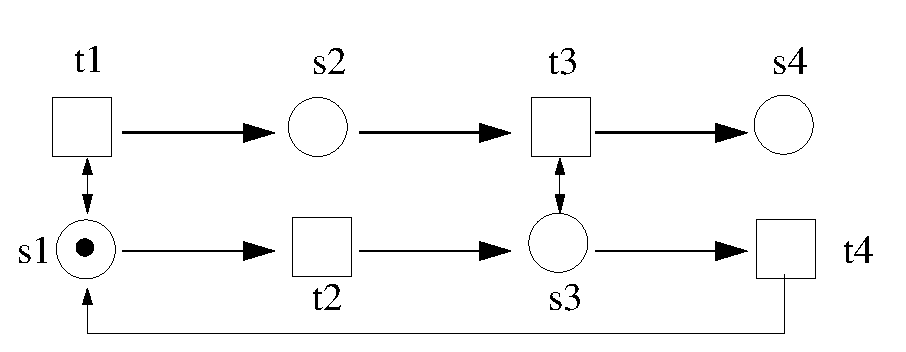
\includegraphics[width=0.5\textwidth]{omegaNet}
%%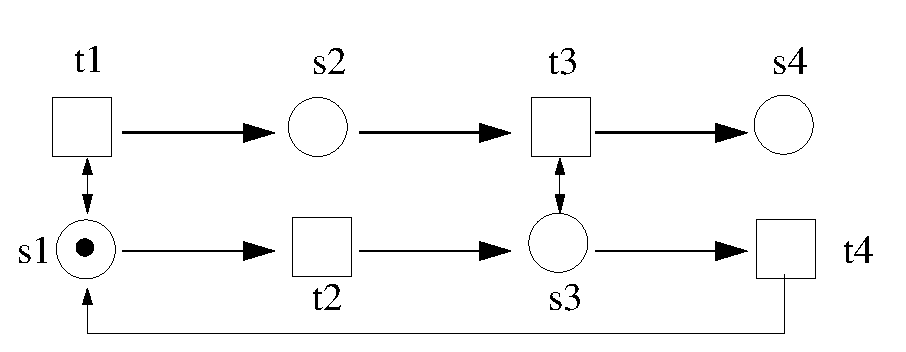
\epsfig{file=omegaNet,width=.5\textwidth}
\caption{A PT-net and configuration with an infinite number of reachable configurations} 
\label{fig:ptnet}
\end{figure}
%

Despite such examples, reachability in PT nets is decidable and can be
determined using an abstraction method called $\omega$-sequences, (see
e.g. \cite{DesR98}).  The main idea in determining $\omega$ sequences
is to define a partial order $\geq_{\omega}$ on configurations as
follows.  If configurations $C_1$ and $C_2$ are both reachable, $C_1$
and $C_2$ have tokens in the same set $PL$ of places, $C_1$ has at
least as many tokens in each place as $C_2$, and there exists a
non-empty $PL_{sub} \subseteq PL$, such that for each $pl \in
Pl_{sub}$ $C_1$ has strictly more tokens than $C_2$, then $C_1
>_{\omega} C_2$.  When evaluating reachability, if $C_2$ is reached
first, and then $C_1$ was subsequently reached, $C_1$ is abstracted by
marking each place in $PL_{sub}$ with the special token $\omega$ which
is taken to be greater than any integer.  If $C_1$ was reached first
and then $C_2$, $C_2$ is treated as having already been seen.

Tabling combined with partial order answer subsumption requires
slightly over 100 lines of code to model reachability in PT nets using
$\omega$-sequences.  Due to space restrictions, the program cannot be
fully described here, but the top-level reachability predicate is
shown in Figure~\ref{fig:ptnetcode}.  Despite its succinctness, it can
evaluate reachability in networks with millions of states in a few
minutes.  This use of tabling to determine reachability in PT nets can
be seen as a special case of tabling for abstract interpretation
(cf. \cite{KaKa93} and other works).  However the framework for answer
subsumption described here allows tabling to be used to efficiently
perform abstract interpretation within a general Prolog system
%
\begin{figure}
\begin{verbatim}
:- table reachable(_,po(omega_gte/2,omega_abs/3)).
reachable(InConf,NewConf):-
        reachable(InConf,NewConf),
        hasTransition(Conf,NewConf).
reachable(InConf,NewConf):- hasTransition(InConf,NewConf).
\end{verbatim}
\caption{Top-level predicate for PT net reachability}
\label{fig:ptnetcode}
\end{figure}

\subsubsection{Scalability for multi-valued and quantitative logics} \label{sec:mv}
\index{tabling!answer subsumption}
%
The technique of program justification (cf. e.g. \cite{PGDRR04}) has
been used for debugging tabled programs that cannot be debugged by
traditional means.  Here, we consider justification in the context of
the Silk system, currently under development at Vulcan, Inc.  Silk is
a commercial knowledge representation and rule system built on top of
Flora-2, which is implemented using XSB.  One of the salient features
of Silk is its default reasoning, which is based on a parameterized
argumentation theory evaluated under the well-founded
semantics~\cite{WGKFL09}.  One issue in using Silk is that knowledge
engineers must have a way of understanding the reasoning of the
system, a task complicated by the use of the well-founded semantics
and the intricacies of the argumentation theory.  We describe an
experimental approach to justification of Silk-style argumentation
theories using multi-valued logics.

As noted in~\cite{WGKFL09}, argumentation theories in Silk are usually
extensions of the default theories of Courteous Logic Programs (CLP)
and are based on two user-defined predicates: {\tt opposes/2} and {\tt
  overrides/2}.  Two atoms {\em oppose} each other if no model of a
program can contain both atoms: an atom and its explicit negation
oppose each other, but opposition can capture many other types of
contradictions.  Given two opposing atoms, one atom may {\em override}
the other, and so be given preference.  For atoms $A_1$ and $A_2$, if
$A_1$ and $A_2$ are both derivable and oppose each other but neither
overrides the other, $A_1$ and $A_2$ mutually {\em rebut} each other.
If in addition $A_1$, say, overrides $A_2$, $A_1$ {\em refutes}
$A_2$~\footnote{In~\cite{WGKFL09} argumentation theories are built on
  named rules, here we base them on derived atoms.}.  Within Silk and
Flora-2, the compilation of an argumentation theory ensures that
rebutted atoms have an undefined truth value, as do atoms that refute
themselves (i.e. if the {\tt overrides/2} predicate is cyclic).
However, for justification, it is meaningful to distinguish those
facts that are undefined due to a negative loop in the argumentation
theory from those that are undefined due to a negative loop in the
program itself.  In addition, it is meaningful to distinguish an atom
that is true because it overrides some other atom, from an atom whose
derivation does not depend on the argumentation theory.  Similar
distinctions can be made for default false literals leading to the
truth lattice shown in Figure~\ref{fig:courteous}.
\begin{figure}
\comment{
\small{
\begin{verbatim}
:- table defeated/1.
defeated(A):-  defeated_by(A,_B).       defeated(A):-  defeats(A,_B).

defeated_by(A,B):- refutes(B,A),B.      defeats(A,B):- refutes(A,B),B.	        
defeated_by(A,B):- rebuts(B,A),B.       defeats(A,B):- rebuts(A,B),B.		

refutes(A,B):- conflicts(A,B), overrides(A,B).
rebuts(A,B):- conflicts(A,B).

conflicts(A,B):- opposes(A,B),A.        conflicts(A,B):- opposes(B,A),A.
\end{verbatim}
}}
\centering
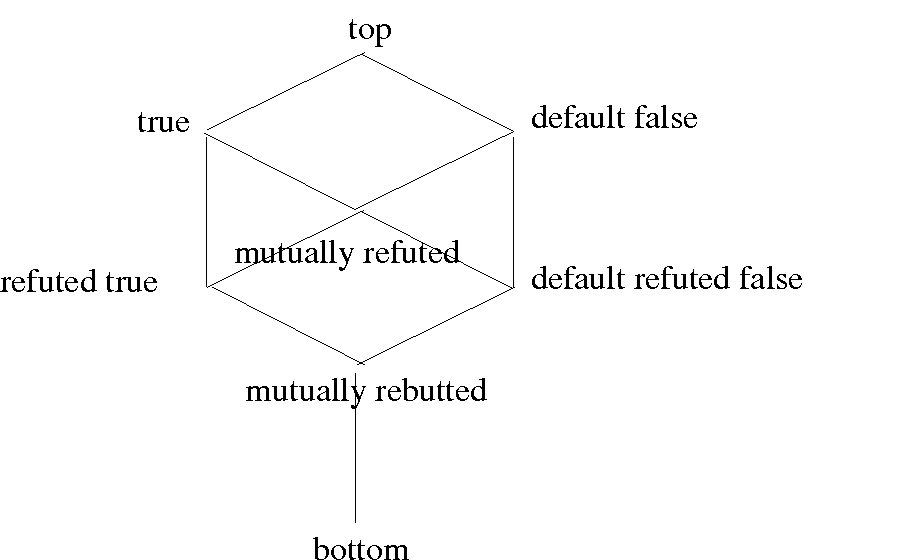
\includegraphics[width=0.45\textwidth]{courteous2}
%%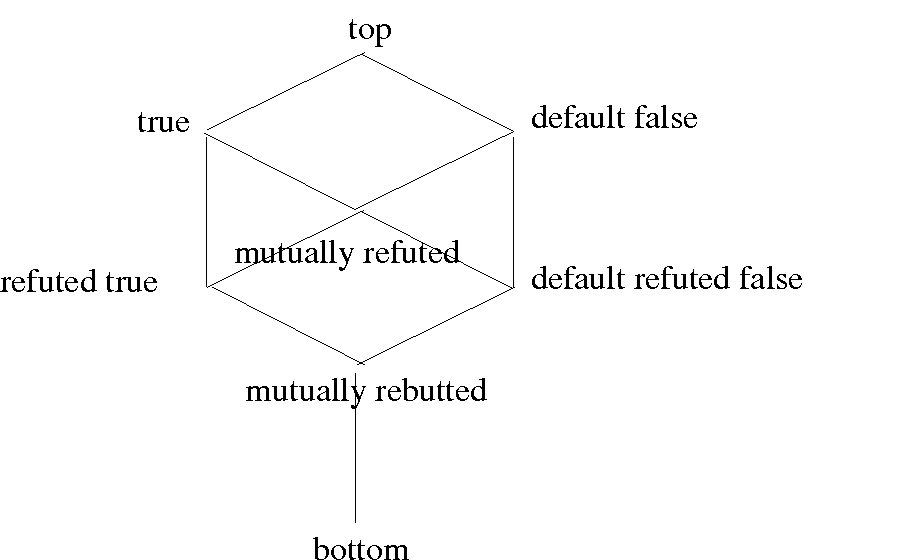
\epsfig{file=courteous2,width=.45\textwidth}
\caption{A Truth Lattice for a Simplified Version of Courteous Argumentation Theory} 
\label{fig:courteous}
\end{figure}
%

\subsection{Term-Sets}

XSB provides support for a programming technique for representing sets
of terms, called term-sets.  (While it is not closely related to
answer subsumption, it is partially implemented through tabling and a
table declaration, and so this facility is documented here.)

We begin in an example.  We can represent a set of Prolog terms by
using a particular term of the form \verb|{Var:Goal}| where Goal has
(only) \verb|Var| free in it.  Then we will use this \emph{set-term} to
represent the set of terms obtained by evaluating \verb|Goal| and
taking the values of \verb|Var| that are obtained.  I.e., they would
be the terms in the list \verb|L| returned by the Prolog call to
\verb|setof(Var,Goal,L)|. For example, the set-term:
\begin{verbatim}
{X : member(X,[a,b,c])}
\end{verbatim}
represents the set of terms \verb|{a,b,c}|.

Now a \emph{term-set} is a Prolog term that may contain set-terms as
subterms.  For example,
\begin{verbatim}
m({X:member(X,[a,b,c])},g(d,{Y:member(Y,[e,f,g])}),h)
\end{verbatim}
is a term-set, and it represents the set of terms obtained from it by
replacing (recursively) any embedded set-term by a term in that
set-term.  So the above term-set represents the 9 terms:
\begin{verbatim}
m(a,g(d,e),h)        m(a,g(d,f),h)        m(a,g(d,g),h)
m(b,g(d,e),h)        m(b,g(d,f),h)        m(b,g(d,g),h)
m(c,g(d,e),h)        m(c,g(d,f),h)        m(c,g(d,g),h)
\end{verbatim}
This example shows an advantage of this representation.  Say a
term-set has $k$ sub-set-terms each of which is of the member form in
this example where each member has a list of atoms of length $n$.  To
represent this set of terms explicitly takes $O(n^k)$ space, whereas
to represent them with the term-set takes only $O(n \times k)$ space.  So a
term-set representation can take exponentially less space than an
explicit representation.

It is relatively easy to write a predicate, {\tt member\_termset/2},
which takes a variable and a term-set
and non\-deterministically generates all concrete terms represented by
the term-set, called \emph{extensionalizing} the term-set.  Some care
must be taken since a call to goal to extensionalize a set-term may
itself return a term-set.  Also term-sets can be self-recursive and
thus represent infinitely many Prolog terms.  For example, consider
the term-set:
\begin{verbatim}
{X : p(X)} where
  p(a).
  p(f({X:p(X)})).
\end{verbatim}
This term-set represents the terms for which {\tt p/1} is true.  Now
{\tt p(a)} is true, so {\tt a} is in the term-set.  Since {\tt a} is
in \verb|{X:p(X)}|, then {\tt p(f(a))} is true because of the second
fact for {\tt p/1}, and so {\tt f(a)} is in the term-set.  And so on.
So this term-set contains the infinitely many terms:
\begin{verbatim}
a, f(a), f(f(a)), f(f(f(a))), ...
\end{verbatim}

A particularly interesting use of term-sets is in conjunction with
tabling.  Consider the term-set \verb|{X:p(1,2,X)}| where {\tt p/3} is
tabled.  If \verb|p(1,2,_}| has been called and so its table is
filled, then extensionalizing this term-set requires just a table
lookup; in some sense we can think of such a term-set as standing for
a pointer into a table to a set of terms.  This can be elegantly used
to solve an important problem in handling parse trees in context-free
parsing.

Consider the following DCG for the language {\tt a}*:
\begin{verbatim}
:- table a/3.
a(a(P1,P2)) --> a(P1),a(P2).
a(a) --> [a].
\end{verbatim}
which recognizes a string of {\tt a's} and constructs its parse trees.

To generate all answers, this DCG will take time exponential in the
length of the input string; not surprising since there are
exponentially many parses.  But say we give it an input string of $n$
{\tt a}'s followed by one {\tt b}.  In this case it will take
exponential time to fail, since it will construct all the
exponentially many partial parse trees for the initial $k$ {\tt a}'s.
We would like the parser in this case to fail in polynomial time.  We
can do this by representing the parse trees as a term-set during the
recognition of the string.  Then after the string is recognized, we
extensionalize the set-term that represents the parse trees.  In this
way we can get the behavior we want.  The set-term that represents the
parse trees for any grammar will be constructed in polynomial time;
the extensionalization of that term-set will take exponential time
only if there are exponentially many parses.

We can cause XSB to automatically use the term-set representation for
the grammar by adding to the above program the declaration:
\begin{verbatim}
:- table a(termset,_,_).
\end{verbatim}
which tells XSB to use the term-set representation of the first
argument of nonterminal {\tt a/3}.

With this declaration, the XSB compiler transforms the above program
into the following:
\begin{verbatim}
:- table a/3.

a(a(P1,P2),S0,S) :- '_$a'(P1,S0,S1),'_$a'(P2,S1,S).
a(a,S0,S1) --> 'C'(S0,a,S1).

:- table '_$a'/3 as subsumptive.
'_$a'({X:'_$a'(X,S0,S)},S0,S) :- a(_,S0,S).
\end{verbatim}
A new predicate {\tt '\_\$a'/3} has been introduced, and all calls to the
original predicate {\tt a/3} are replaced by calls to the new one.  It
is defined to call the original {\tt a/3} but to return the term-set
instead of the concrete parse tree in the argument declared to be a
term-set.

We can see that a call to {\tt a/3} in this new program will have
exactly as many answers as the corresponding call to {\tt a/2} in the
original recognizing DCG, since given values for {\tt S0} and {\tt S},
a call to {\tt '\_\$a'/2} returns only one value in its first
argument.  So a call to {\tt a/3} with have the polynomial complexity
of the recognizer.  So now when this representation is used, one gets
the concrete parse tree for a string by writing, for example:
\begin{verbatim}
| ?- a(Pts,[a,a,a,a,a,a,a],[]), member_termset(Parse,Pts).
\end{verbatim}
Here the term-set representing the parses for the sequence of {\tt
a}'s will be returned in the variable {\tt Pts}, and then {\tt
member\_termset} is used to extensionalize it
to the produce the actual explicit parse
tree.  With this way of handling parse trees in arbitrary context-free
grammars, the complexity of parsing to create the term-set is always
polynomial, and then extensionalizing the term-set may be exponential
if all parses are desired and there are exponentially many of them.
(In fact, if the grammar contains a rule such as \verb|A --> A|, there
may be infinitely many parses.)
Of course, if the parsing call to {\tt a/3} fails, then there is no
extensionalization to do, and the process is polynomial.

Note that the transformation uses subsumptive tabling for the newly
introduced auxiliary predicate.  This is important for this example,
since the parsing calls to {\tt '\_\$a'/3} will normally have {\tt S0}
bound and {\tt S} free, yet when extensionalizing the constructed
term-set to obtain the parse trees, the calls will have both {\tt S0}
and {\tt S} bound.  We do not want to recompute the parse during
extensionalizion, which would happen were we to use variant
tabling, and so we use subsumptive tabling.

Problems in graph traversal provide another example of the effective
use of term-sets.  For graph reachability, we have the very familiar:
\begin{verbatim}
:- table reach/2.
reach(X,Y) :- edge(X,Y).
reach(X,Y) :- reach(X,Z), edge(Z,Y).
\end{verbatim}
which is linear in the number of edges in the graph.  But say that we
now want to construct the path from X to Y when Y \emph{is} reachable
from X.  One simple way to do it (collecting the intermediate nodes in
the path in reverse order) is:
\begin{verbatim}
:- table path/3.
path(X,Y,[]) :- edge(X,Y).
path(X,Y,[Z|Path]) :- path(X,Z,Path), edge(Z,Y).
\end{verbatim}
For an acyclic edge graph, this works fine, but for a graph with
cycles, this will go into an infinite loop.  Indeed, it must, since in
a cyclic graph there \emph{are} infinitely many different paths between
some nodes.  However, we can use term-set to handle this situation
more flexibly.  We modify the above program by adding:
\begin{verbatim}
:- table path(_,_,termset).
\end{verbatim}
With this declaration, every call to {\tt path/3} (for a finite edge
graph) will terminate in time linear in the number of edges.  And all
the paths will be presented in the term-set returned in the third
argument.  Here we have an advantage similar to the one we had in the
grammar example above: if there is no path from our source to our
target node, we will find that out in linear time.  Without the
term-set declaration, this might take exponential time, while the
program builds all the paths to all the nodes that \emph{are} reachable
from our source node.  Also, if we want only \emph{one} possible path
from our source to our target, we can easily retrieve only one member
of the term-set during extensionalization, and the whole process is
still linear.

Now consider what happens with when the graph has cycles.  In this
case, the term-set may be recursive and represent the infinitely many
paths between nodes.  For example, the term-set representing all paths
from {\tt a} to {\tt a} in the graph with a single edge from {\tt a} to
{\tt a} will have the same structure as the example of an infinite
term-set given at the beginning of this subsection.  Once the path
term-set is constructed (in time linear in the number of edges for a
single source), producing paths reduces to processing the term-set
structure.  For example to generate all paths between nodes which do
not contain repeated intermediate nodes, one could write an
extensionalization predicate that passes a list of term-sets in the
process of being expanded, and refuse to re-expand one currently being
expanded.  This is the technique often used in Prolog without tabling
to compute reachability in cyclic graphs.

All of these examples can be seen as special cases of constructing
proof trees or justifications of goals.  Indeed, term-sets could be
effectively used in the construction of a justification or explanation
system.

\index{termination!subgoal abstraction}
\index{bounded rationality}
\index{termination!radial restraint}
\index{termination!answer count restraint}
\index{abstraction of terms!subgoal}
\index{abstraction of terms!answer}
\section{Tabling for Termination} \label{sec:tabling-termination}
%
As noted throughout this manual, tabling adds important termination
properties to programs and queries.  In this section we state more
precisely what these termination properties are, and how the
properties can be strengthened through declarations and settings for
{\em subgoal abstraction} and for sound bounded rationality through a
type of answer abstraction called {\em radial restraint} as well as by
limiting the number of answers to a subgoal through {\em \maxans{}
  restraint}.

Before proceeding, it is important to set the context for where issues
of termination may arise.  Consider first a pure normal program in
which every predicate is tabled.  This means a program where rules may
only call other rules, possibly through negation ({\tt tnot/1}, {\tt
  not\_exists/1} or {\tt u\_not/1} in XSB); but where there are no
calls to built-in all-solutions predicates, or other built-ins.  If
such a fully-tabled pure normal program does {\em not} have function
symbols, XSB will always terminate for any query.  For instance, XSB
will terminate for fully tabled pure datalog programs -- even if the
head of a rule is ``unsafe'' in that it contains variables that do not
occur in the body of that rule~\footnote{Evaluations that call
  non-ground negative literals will terminate through floundering,
  although this can be avoided in most cases by using {\tt
    not\_exists/1}.}.  Such programs are sometimes called \emph{datalog}
programs.

While datalog programs are useful for certain kinds of knowledge
representation, they are not powerful enough for general programming
as they do not allow recursive structures such as lists.  Thus, for
the rest of this section we consider pure programs that may contain
function symbols.  Consider a pure definite program in which every
predicate is tabled.  Such a program would create a table for each
tabled subgoal (up to variance) exactly once if call variance were
used, and at most once if call subsumption were used.  In addition,
tabling guarantees that each answer will be returned to each call to a
tabled subgoal at most once.  This means that there are two sources of
non-termination.  Either there can be an infinite number of subgoals,
or there can be an infinite number of answers.\footnote{Here, forest
  of trees model of tabling (cf. Section~\ref{sec:forest-trace}) is
  being implicitly used.}

\paragraph{An Infinite Number of Subgoals}
%
If a definite program produces an infinite number of subgoals {\em
  but} has a finite number of answers, the program can be made to
terminate by abstracting the subgoal.  For instance, consider the
program fragment:
%
\begin{verbatim}
:- table p/1.
p(X) :- p(f(X)).
\end{verbatim}
%
The goal {\tt ?- p(1)} can create an infinite number of tabled
subgoals: {\tt p(f(1))}, {\tt p(f(f(1)))}, {\tt p(f(f(f(1))))} and so
on.  Note that since all of the subgoals are ground, none subsume one
another, so that call subsumption will not help here. (Although call
subsumption is extremely useful in other circumstances, and would terminate
if the goal were {\tt ?- p(X)}).

\paragraph*{Infinite Answers}
%
Of course, subgoal abstraction can't handle cases where there are an
infinite number of answers, as in the program fragment:
%
\begin{verbatim}
p(f(X)) :- p(X).
p(1).
\end{verbatim}
%
when given the query {\tt ?- p(X)}.  

We consider each case in turn.

\subsection{Term Size Abstraction in XSB} \label{sec:size-metric}
\index{abstraction of terms!size metric}
%
Both subgoal and answer abstraction in XSB are based on limiting the
size of any argument of a term $T$ that forms a subgoal or answer.
The specific definition of size used is slightly complicated, but
offers advantages as discussed below.  Each argument $T_a$ of $T$ is
traversed as follows.  The size of $T_i$ is initialized to 0, then
$T_a$ is traversed from left to right.  Each time a non-constant
functor or list symbol is encountered, the size of $T_i$ is
incremented by 1 -- regardless of the type of functor symbol that is
encountered.  If the size of $T_a$ exceeds the associated size limit
for $T$ (as declared in the next section), all further non-constant
functor symbols encountered in $T_i$ will be abstracted (rewritten as
free variables).  Once $T_a$ has been fully traversed, further
arguments of $T$ will be traversed in the exact same manner.

%, with one
%important exception.  The functor symbols will be abstracted {\em
%  only} if they also occur at depth greater than 0.

\begin{example} \label{ex:term-size-abs}
Applying the above definition of size abstraction with limit 2 to the
term 

{\tt p(d(e(1),a,f(c$_1$)),b,g(c$_2$),[c$_3$,[c$_4$,c$_5$]]))}

\noindent
  produces the term 

{\tt p(d(e(X$_1$),a,X$_2$),b,g($c_2$),[$c_4$|X$_3$])}.  

\noindent
In the traversal, the size limit is reached once the {\tt e/1} functor
is encountered.  To the right of {\tt e/1}, all non-constant functor
symbols are abstracted when they occur at depth greater than 0.  This
causes {\tt f/1} to be abstracted, as it occurs at depth 1; however
{\tt g/1} in the third occurs at depth 0, and so is retained.
Similarly in the fourth argument, the outer list symbol and head is
preserved, while the tail of the list is abstracted.
\end{example}

Example \ref{ex:term-size-abs} indicates that the size abstraction
used in XSB excludes symbols of depth 0, and so is something of a
hybrid approach, although we continue to call it size abstraction.

Other metrics could be used, such as term depth, which would offer
conceptual clarity.  However size-based abstraction allows
finer-grained optimization than depth-based abstraction and offers the
following general advantages.
\begin{itemize}
\item From the point of view of implementation, the abstraction can be
  performed with manner that has minimal if any impact on the speed of
  XSB's tabling engine.
\item By not abstracting functor symbols at depth 0 and by abstracting
  each argument individually, both multi-argument indexing and star
  indexing of subgoals will be often be preserved.
\end{itemize}

\subsection{Subgoal Abstraction} \label{sec:subg-abs}
\index{abstraction of terms!subgoal}
%
In a nutshell, subgoal abstraction allows a goal like {\tt
  p(f(f(f(1))))} to be rewritten as 

{\tt p(f(f(X))),X = f(1)}.  

\noindent
If all subgoals that have a term size -- or term depth -- over a given
finite threshold are abstracted, any query can produce only a finite
number of subgoals (since there are a finite number of predicate,
function and constant symbols in any program). If a program has a
finite well-founded model, it can be shown that any query to a program
will terminate if that program uses subgoal abstraction~\cite{RigS14}.
%
For normal programs, the situation is not much different at a
conceptual level.  A goal such as {\tt tnot(p(f(f(f(1)))))} would
execute as {\tt p(f(f(X)))} and then ensure that none of the answers
to this goal have a binding for {\tt X} that allows it to unify with
{\tt f(1)}.  Using this intuition, it can be shown that if a program
has a well-founded model with a finite number of true or undefined
answers it will terminate using tabling with subgoal
abstraction~\cite{RigS13,RigS14}.

Despite its theoretical power, subgoal abstraction can also cause
problems if used indiscriminately.  For instance, if the second
argument of the subgoal
%
\begin{verbatim}
?- member(e,[a,b,c,d,e])
\end{verbatim}
%
is abstracted forming the goal
%
\begin{verbatim}
?- member(e,[a,b,c|X])
\end{verbatim}
%
leading to an infinite number of answers.  a goal that terminates
without abstraction will not terminate after abstraction.  Note that
any program containing {\tt member/2} and at least one constant does
not have a finite model (although any given ground query will have a
finite number of answers).  While an experienced programmer would not
usually table {\tt member/2}, s/he well may want to table a grammar or
other program that performs recursion through a finite structure.

\index{tripwires!max\_table\_answer\_size}
\subsubsection{Declaring Subgoal Abstraction}
%
% The implementation of subgoal abstraction in XSB is still in progress.
% and may be changed in future versions as we gain experience in how
% subgoal abstraction is best used in practice.  

XSB can perform subgoal abstraction based on the size limit described
above.  It will do so for goals called positively, but not for goals
called negatively as this would give rise to unsound negation.  Thus a
goal $G$ inside a construct such as {\tt tnot/1} or {\tt
  not\_exists/1} will throw an exception (or suspend into break mode)
if it surpasses the specified term size. In addition, subgoal
abstraction is only implemented for call variance, {\em and applies
  equally to all functors, whether they are lists or non-lists}.
Despite these restrictions, a tabled evaluation can be still
guaranteed to terminate for queries to safe programs
(cf.~\cite{RigS13}).

\index{Prolog flags!{\tt max\_table\_subgoal\_action}} 
\index{Prolog  flags!{\tt max\_table\_subgoal\_size}} 

Subgoal abstraction can be declared by setting a value for the maximum
size of a subgoal and for the action to take when a subgoal is
encountered that reaches that size.
%
\bi
\item {\bf size} The maximum size can be set to $n$ for a set of
  predicates $\langle PredSpec \rangle$ by including the specifier
  {\tt subgoal\_abstract(n)} as part of the tabling declaration

{\tt :- table $\langle PredSpec\rangle$  as ...,subgoal\_abstract(n),...}

  Specifying {\tt subgoal\_abstract(0)} turns abstraction off for
  predicates in $\langle PredSpec \rangle$.  The size can also be set
  globally by setting the flag {\tt max\_table\_subgoal\_size} to the
  desired maximal size.  If the subgoal size has been set of a given
  predicate via a tabling declaration the declared size will override
  the global size.

\item {\bf action} When a subgoal is encountered of maximum size,
  abstraction is enabled if the Prolog flag {\tt
    max\_table\_subgoal\_action} to {\tt abstract}.  Other possible
  values for the action are {\tt error} and {\tt suspend}
  (cf. pg. \pageref{prolog-flags} ff.).  \ei

\noindent
Unless otherwise specified, XSB starts up with {\tt
  max\_table\_subgoal\_action} set to {\tt error} and {\tt
  max\_table\_subgoal\_size} set to 0, indicating it is turned off.
Under this default behavior, XSB will throw an error if a subgoal has
size greater than {\tt max\_table\_subgoal\_size}.  As an alternative
to setting flags, subgoal abstraction can be set by calling XSB with
the command-line arguments {\tt --max\_subgoal\_action a} and {\tt
  --max\_subgoal\_size n} with {\tt a} the desired action and {\tt n}
the desired size limit.

\subsection{XSB's Approach to Bounded Rationality} \label{sec:restraint}
\index{abstraction of terms!answer}
\index{bounded rationality}
%
Bounded rationality is a subfield of Artificial Intelligence that
studies how the reasoning performed by a computation can be
automatically bounded so that an agent or other program can be
guaranteed to arrive at a decision ``quickly''.  By bounding
reasoning, an agent may be used in a setting that requires reactivity
or where a simulation of human reasoning is needed.

%Thus, the approximation that XSB computes is {\em
%  informationally sound} in the sense that no incorrect answer will be
%derived, although the truth value of some atoms won't be known that
%might have been if the size bound had been set higher.  

XSB's approach to bounded rationality computes a finite approximation
to the well-founded model that is {\em informationally sound} in the
sense that no incorrect answer will be derived, although the truth
value of some atoms won't be known. In other words, if bounded
rationality is employed, it can be guaranteed that only a finite
number of answers will be derived~\cite{GroS13}.  Furthermore, any
true atom that XSB derives is true in the well founded model of a
program; and any goal that fails is false in the well-founded model.
However, by bounding rationality XSB's search is restrained so that it
will not fully explore certain subderivations and so may consider as
undefined some atoms that are true or false in the well-founded model.
We sometimes call this approach to bounded rationality {\em
  restraint}.  Currently XSB supports both {\em radial restraint} and
{\em \maxans{} restraint}

\index{restraint!radial}
\subsubsection{Radial Restraint Through Answer Abstraction}
Radial restraint resembles subgoal abstraction (Section
\ref{sec:subg-abs}) in certain ways, as can be seen in the following
example. If the query {\tt p(X)} to the program
%
\begin{verbatim}
p(f(X)) :- p(X).  
p(0).
\end{verbatim}
%
were evaluated using radial restraint with a size limit of 3, the
answers, {\tt p(0)}, {\tt p(f(0))}, {\tt p(f(f(0)))} and {\tt
  p(f(f(f(X))))} would be generated; {\bf {\em however}}, {\tt
  p(f(f(f(X))))} would have the truth value of {\em undefined}.  Note
that by abstracting in this way, both of the goals {\tt
  p(f(f(f(0))))}, and {\tt p(f(f(f(1))))} will unify with {\tt
  p(f(f(f(X))))} and so will succeed with a truth value of {\em
  undefined}.  Similarly {\tt tnot(p(f(f(f(0)))))}, and {\tt
  tnot(p(f(f(f(1)))))} will both succeed with a value of {\em
  undefined} (perhaps better called {\em unknown} in this context).
%
It can be seen that since all predicates and function symbols have a
maximum arity (256 in XSB) bounding the size of an answer ensures that
only a finite number of answers are returned
\footnote{If a program has a infinite number of true answers and a
  finite number of false answers, one possible approach might be to
  ``dualize'' the program so that only false answers are computed.
  Note that since most programs with function symbols have an infinite
  number of both true and false answers, this approach won't work in
  general.}.

Semantically when radial restraint is used, XSB computes an
approximation to the three-valued well-founded model of a program,
called a {\em restrained model}.  To see this, suppose the proof of a
query $Q$ does not depend on negation.  If $Q$ has a derivation that
does not require any answers whose size is greater than $n$, it is
proven as usual.  Similarly, if $Q$ is false in the well-founded model
of a program, and none of the subgoals explored in the derivation of
$Q$ derive answers whose size is greater than $n$, XSB will derive
that $Q$ is false.  The higher the size bound that is set, the better
the approximation.  Due to undecidability, there is no way to know in
general what size to set for answer abstraction, or whether any bound
needs to be set at all.

If a restrained model is derived, answers that are directly undefined
through radial restraint can be distinguished from answers that are
undefined in the well-founded model of a program, or for other reasons
such as unsafe negation.  If an answer $A$ was abstracted due to a
size check, the query {\tt get\_residual(A,Delay)} would bind {\tt
  Delay} to a list containing the atom {\tt radial\_restraint}, where
{\tt radial\_restraint/0} is simply a predicate defined as

{\tt radial\_restraint:- tnot(radial\_restraint)}

%\noindent
%which in a delay list indicates that an answer was made undefined
%through bounded-rationality based answer abstraction.

\index{tripwires!max\_table\_answer\_size}
\paragraph*{Using Radial Restraint}
%
Radial restraint is currently implemented only for tabling with call
variance.  However it works with most other tabling features, such as
call abstraction, and incremental tabling.
%
Similarly to the use of subgoal abstraction, answer abstraction is the
implementational basis of radial restraint.  As shown in the following
example, {\em it is important to note that the size limit applies to
  the answer substitution, not to the size of the answer itself.}

\begin{example}
Suppose an answer size limit is set to 1, and consider the goal {\tt
  p(X)}.  The answer {\tt p(s(s(0)))} has size 2 and so would be
abstracted to {\tt p(s(X$_1$))} as expected, as the corresponding
abswer substitution is $X = s(s(0))$.  However for the goal {\tt
  p(s(X))} the answer substitution for the answer {\tt p(s(s(0)))} is
$X = s(0)$ which has a size of only 1 and so this answer would not be
abstracted in the context of this subgoal.  Despite this difference in
how the size metric is computed, the termination and approximation
properties of radial restraint still hold.
\end{example}

Radial restraint can be declared by setting a value for the maximum
size of an answer and for the action to take when an answer is
encountered that reaches that size.
%
\bi
\item {\bf size} The maximum size can be set to {\tt n} for a set of
  predicates by including the specifier {\tt answer\_abstract(n)} as
  part of their tabling declaration

{\tt :- table $<PredSpec>$ as ...,answer\_abstract(n),...}

  Specifying {\tt answer\_abstract(0)} turns answer abstraction off
  for predicates in $\langle PredSpec \rangle$.  The size can also be
  set globally by setting the flag {\tt max\_table\_answer\_size} to
  the desired maximal size.  If the answer size of a given predicate
  has been set via a tabling declaration, the predicate-specific
  declared size will override the global size.

\item {\bf action} When an answer is encountered of maximum size,
  abstraction is enabled if the Prolog flag {\tt
    max\_table\_answer\_action} to {\tt abstract} (or, equivalently,
  to {\tt bounded\_rationality}).  Other possible values for the
  action are {\tt error}, {\tt suspend} and {\tt custom} (cf. Section
  \ref{sec:tripwire} for further information).  \ei


\index{Prolog flags!{\tt max\_table\_answer\_action}} 
\index{Prolog flags!{\tt max\_table\_answer\_size}}
%
Unless otherwise specified, XSB starts up with {\tt
  max\_table\_answer\_size\_action} set to {\tt error} and {\tt
  max\_table\_answer\_size} set to 0.  
%

\subsubsection{\MAXANS{} Restraint} \label{sec:answer-count-restraint}
\index{tripwires!max\_answers\_for\_subgoal}
\index{restraint!answer count}

As discussed above, finite termination -- and some types of bounded
rationality -- can always be ensured through a mixture of subgoal
abstraction and radial restraint.  Alternately, these features can
also be ensured through subgoal abstraction and \maxans{} restraint.

\begin{example} \label{ex:maxans}
Consider the program

\begin{verbatim}
:- table p/4.
p(M,N,X,Y):- between(1,M,X),between(1,N,Y).
\end{verbatim}

\noindent
and query {\tt p(3,3,Y,Z)}: it is easy to see that 9 answers will be
produced.  However, if \maxans{} restraint is used to restrict the
maximal number of answers to each subgoal to 5, the first 5 answers
computed above will be returned, along with a new answer:

{\tt p(3,3,Y,Z)}

\noindent
whose truth value is undefined, with the atom 
%
{\tt \maxUans\_restraint} in its delay list.
\end{example}

Using the arguments from the previous section, it is easy to see that
\maxans{} restraint ensures sound finite termination when used with
subgoal abstraction.  However Example~\ref{ex:maxans} also illustrates
on a small scale how \maxans{} restraint can be used to soundly
complete a subgoal $S$ once a minimal number of answers have been
derived, even if $S$ has a large, but finite number of answers.

\paragraph*{Using \MAXANS{} Restraint}
\Maxans{} restraint is currently implemented only for tabling with call
variance.  However it works with most other tabling features, such as
call abstraction, and incremental tabling.

Currently, \maxans{} restraint can only be set by global flags as
follows.
\bi
\item {\bf size} The size can be set globally via the flag {\tt
  max\_table\_answer\_size} to the desired maximal size.  Setting the
  flag to 0 turns off \maxans{} restraint.

\item {\bf action} When an answer is encountered of maximum size,
  abstraction is enabled if the Prolog flag {\tt
    max\_table\_answer\_action} to {\tt complete\_soundly}.  Other
  possible values for the action are {\tt error}, {\tt suspend} and {\tt custom}
  (cf. Section \ref{sec:tripwire} for further information).  \ei

\subsubsection{Justifying or Explaining Restraint}

An atom affected directly by radial or answer count restraint has in
its delay list either the atom {\tt radial\_restraint} or {\tt
  answer\_count\_restraint}.  The indirect dependency of an atom on a
form of restraint can be obtained either through the predicate {\tt
  explain\_u\_val/3}, or {\tt get\_residual\_sccs/[3,5]}.  Both of
these predicates traverse the residual dependency graph to provide
information about why a literal is undefined.

\index{residual dependency graph}
\predref{explain\_u\_val/3}
\predref{get\_residual\_sccs/3}
\predref{get\_residual\_sccs/5}

%--------------------------------------------------------------------
\section{Incremental Table Maintenance} \label{sec:incremental_tabling}
%====================================================

\index{tabling!incremental}

XSB allows the user to declare that the system should maintain the
correctness of a given table with respect to dynamically changing
facts and rules through so-called {\em incremental
  tables}~\cite{SaRa05,Saha06,Swif14}.
%A table $T$ is {\em incremental} if XSB ensures that its answers are
%  consistent with all dynamic facts and rules upon which $T$ depends
%  (subject to transactionality conditions explained below).
After a database update or series of updates $\Delta$, an incremental
table $T$ that depends on $\Delta$ is by default updated
transparently: that is $T$ and all tables upon which $T$ depends are
automatically updated (if needed) whenever a future subgoal calls $T$.
%Alternately, if circumstances require it, a table can be updated
%immediately upon a database change or by issuing an explicit command
%to update all tables that depend on $\Delta$.
%
In either case, incremental tabling brings XSB closer to the
functionality of deductive databases.  If tables are thought of as
materialized database views (or snapshots), then the incremental table
maintenance subsystem enables incremental view maintenance; also as
discussed below, if choice points are thought of as database cursors
then incremental tabling also provides view consistency~\footnote{In
  the current version of XSB, there are certain restrictions on how
  incremental tabling can be used:
  cf. Section~\ref{sec:tabling-compatibility}.}.

\subsection{Transparent Incremental Tabling} \label{sec:incr_examples}

To demonstrate incremental table maintenance (informally called {\em
  incremental tabling}), consider first the following simple program
that does not use incremental tabling:
\begin{verbatim}
:- table p/2.
p(X,Y) :- q(X,Y),Y =< 5.

:- dynamic q/2.
q(a,1).    q(b,3).   q(c,5).    q(d,7).
\end{verbatim}
and the following queries and results:
\begin{verbatim}
| ?- p(X,Y),writeln([X,Y]),fail.
[c,5]
[b,3]
[a,1]

no
| ?- assert(q(d,4)).

yes
| ?- p(X,Y),writeln([X,Y]),fail.
[c,5]
[b,3]
[a,1]

no
\end{verbatim}
%
In this program, the table for {\tt p/2} depends on the contents of
the dynamic predicate {\tt q/2}.  We first evaluate a query, {\tt
  p(X,Y)}, which creates a table.  Then we use {\tt assert/1} to add a
fact to the {\tt q/2} predicate and re-evaluate the query.  We see
that the answers haven't changed, because the table is already created
and the second query just retrieves answers directly from that
existing table.  However the answers are inconsistent with the model
of {\tt p/2} after the assert.  I.e., if the table didn't exist
(e.g. if {\tt p/2} weren't tabled), the answer {\tt [d,4]} would also
be derived.  Without incremental table maintenance, the only solution
to this problem is for the XSB programmer to explicitly abolish a
table whenever changing (with assert or retract) a predicate on which
the table depends.
%
By declaring that the tables for {\tt p/2} should be incrementally
maintained, XSB automatically keeps the tables for {\tt p/2} correct.

%
Consider a slight rewrite of the above program:
\begin{verbatim}
:- table p/2 as incremental.
p(X,Y) :- q(X,Y),Y =< 5.

:- dynamic q/2 as incremental.
q(a,1).    q(b,3).    q(c,5).     q(d,7).
\end{verbatim}
in which {\tt p/2} is declared to be incrementally tabled
% (with {\tt  :- table p/2 as incremental}) 
and {\tt q/2} is declared to be both dynamic and incremental, meaning
that an incremental table depends on it.
%~\footnote{The declarations {\tt use\_incremental\_tabling/1} and
%  {\tt use\_incremental\_dynamic/1} are deprecated from Version 3.3 of
%  XSB forward -- in other words backwards compatibility will be
%  maintained for a time, but these declarations will not be further
%  supported.}.  
Consider the following goals and execution:
\begin{verbatim}
| ?- import incr_assert/1 from increval.
yes
| ?- p(X,Y),writeln([X,Y]),fail.
[c,5]
[b,3]
[a,1]

no
| ?- incr_assert(q(d,4)).

yes
| ?- p(X,Y),writeln([X,Y]),fail.
[d,4]
[c,5]
[b,3]
[a,1]

no
\end{verbatim}
\noindent
\index{Incremental Dependency Graph (IDG)}
\index{tabling!incremental!invalid subgoals}
The transparent approach to incremental updating works as follows.
When {\tt incr\_assert/1} is called, it sparks an invalidation
phase in which tables that depend on {\tt q(d,4)} are marked as {\em
  invalid} (i.e., possibly inconsistent with respect to underlying
dynamic code).  An {\em Incremental Dependency Graph (IDG)} is used to
obtain the right tables to invalidate.  However, if the invalidation
phase finds an affected table that is incomplete, a permission error
is thrown, since it is unclear whether sensible semantics can be given
to updating a subgoal that is incomplete.  After the invalidation
phase is completed, when/if a subgoal calls an invalid table $T$ the
engine interrupts itself to recompute $T$ and any tables upon which
$T$ depends.  On the other hand, if no calls are ever made to an
invalid incremental table $T'$, $T'$ will never incur the cost of an
update.

\index{view consistency}
\subsubsection{View Consistency} \label{sec:view-consistency}
%
As described above, transparent incremental tablings's use of lazy
updating ensures that a new query $Q$ will always be consistent with
the state of the dynamic code at the time $Q$ is called.  However,
transparent incremental tabling enforces a stronger property of view
consistency similar to those of database systems: that answers to a
query $Q$ should be those derivable at the time $Q$ was called, {\em
  and should not be affected by any updates}.
%Accordingly, the ISO standard for Prolog~\cite{ISO-Prolog} specifies
%that an update $\upsilon$ to dynamic code should not affect the
%behavior of choice points that were created before $\upsilon$.
Because XSB's incremental tabling does not allow updates that affect
tables that are still being computed, supporting view consistency
effectively means ensuring consistency for choice points into
completed incremental tables.  As such choice points correspond to
database cursors, we term them {\em Open Cursor Choice Points,
  (OCCPs)}.

XSB's support for view consistency is designed so that no perceptible
overhead in incurred if there are no OCCPs whose view needs to be
maintained.  Not surprisingly, numerous long-lived OCCPs whose views
need to be maintained across updates causes an overhead for the
engine, a situation that is in some sense similar to the cost of
maintaining views for cursors in database system.

%----------------------------------------------------------------
\comment{
In addition to the success continuations that are standard in most
languages, Prolog has failure continuations -- choice points to take
upon backtracking.  The presence of these failure continuations leads
to an issue of view consistency, even within a single-threaded
computation.  Suppose that a user
%
\begin{enumerate}
\item Makes a query to a completed incrementally tabled subgoal $Q$.
  $Q$ has more than one solution and the first one is returned,
  leaving a choice point into the table for $Q$.
\item Makes an update to dynamic code upon which $Q$ depends
\item Makes another query to $Q$
\end{enumerate}
%
What is the relation between the queries and the update.  Presumably,
the first query in step 1) should not reflect the changes made in step
2) if a user backtracks for further answers to that query -- this can
be seen as ensuring view consistency.. However it is less clear
whether the second query to $Q$ in step 4) should return the same
answers as the first query in step 1), or whether the second query
should reflect the database update.  Arguments can be made for either
approach.
%
\begin{itemize}
\item {\em Prolog-style semantics} If the second query reflects the
  database change, it is consistent with the database, but is not
  consistent with the first query~\footnote{This approach could be
    viewed as an extension of the ISO semantics for dynamic code in
    Prolog, which XSB does not currently support.};
\item {\em Delayed update semantics} If the second query does not
  reflect the dynamic code change, it is consistent with the first
  query but not with the dynamic code change.
\end{itemize}
%
XSB chooses the latter of these approaches.  If a user has failure
continuations into a query $Q$, then $Q$ and all tables that depend on
$Q$ will not be updated until these failure continuations have been
exhausted or removed.  However, all updates are ensured to be applied
once this is the failure continuations are removed.
}

%----------------------------------------------------------------

\subsection{Updating in a Three-Valued Logic}
%
As discussed earlier in this chapter, answers that are undefined in
the well-founded semantics are represented as conditional answers.
Beginning with version 3.3.7, incremental updates work correctly with
conditional answers~\footnote{Before Version 3.3.7, incremental
  updates only worked correctly on stratified tables: those with only
  unconditional answers.}.  Nno special care needs to be taken for
updating in the well-founded semantics as the following example
illustrates.
%conditional answers, and they can be updated through any of the
%previously described methods.  The following example illustrates one
%such approach.

\begin{verbatim}
:- dynamic data/1 as incremental.

:- table opaque_undef/0 as opaque.
opaque_undef:- tnot(opaque_undef).

:- table p/1 as incremental.
p(_X):- opaque_undef.
p(X):- data(X).
\end{verbatim}
%
Note that {\tt opaque\_undef/1} upon which {\tt p/1} depends is
explicitly declared as opaque~\footnote{An {\em opaque} predicate $P$
  is tabled and is used in the definition of some incrementally tabled
  predicate but should not be maintained incrementally.  In this case
  the system assumes that the programmer will abolish tables for $P$
  in such a way so that re-calling it will always give semantically
  correct answers.}.  When the above program is loaded, XSB will
behave as follows.
%
{\small
\begin{verbatim}
| ?- p1(1).

undefined
| ?- incr_assert(data(1)).

yes
| ?- p1(1).

yes
| ?- incr_retract(data(1)).

yes
| ?- p1(1).

undefined
| ?- get_residual(p1(1),C).

C = [opaque_undef]
\end{verbatim}
}
%

%\subsection{Eager Incremental Tabling}~\label{sec:incr-eager}
%%
%Despite the advantages of transparent incremental tabling, there are
%special circumstances when it may be better to update tables eagerly
%rather than when (and if) they are called.  For instance, if updates
%and queries are expected to occur at different times, performing eager
%updates may improve query time.  In addition, if incremental tables
%are accessed via table inspection predicates
%(cf. Chapter~\ref{sec:TablingPredicates}) rather than by queries,
%inconsistent answers may be obtained.  
%
%\paragraph{An Eager Updating Approach}
%%
%Usually, best way to eagerly update tables is to use the {\tt
%  incr\_assert/1} and {\tt incr\_retract(all)/1}
%predicates as discussed above.  When the updates are finished, the
%ommand {\tt incr\_table\_update/0} is then called, which updates all
%tables that depend on any changed dynamic rules or facts.  The
%following execution for our running program shows an example of this.

%\begin{verbatim}
%| ?- import incr_assert/1, incr_table_update/0 from increval.

%yes
%| ?- p(X,Y),writeln([X,Y]),fail.
%[c,5]
%[b,3]
%[a,1]
%%
%no
%| ?- incr_assert(q(d,4)), incr_assert(q(d,1)), 
%
%yes
%| ?- incr_table_update.
%
%| ?- p(X,Y),writeln([X,Y]),fail.
%[d,4]
%[d,1]
%[c,5]
%[b,3]
%[a,1]
%
%no
%\end{verbatim}
%\noindent
%As discussed, calling {\tt incr\_table\_update} causes the cost of
%updating incremental tables to be immediately incurred, and ensures
%that table inspection primitives show correct results.  However,
%tables are updated and their views preserved even if the tables may
%not be accessed before further updates are made.
%
%\paragraph{Issues with Eager Updating}
%%
%In the current version of XSB, eager updating is taken to be something
%of a special use case.  In order to perform eager updating, a global
%update list is maintained whenever changes are made to incremental
%dynamic predicates or tries.  In particular, the list is not updated
%when incremental tables are abolished, so that if an incremental table
%has been abolished making the global update list possibly invalid,
%%eager updating will be disabled for the rest of the session (unless
%{\tt abolish\_all\_tables/0} is called.  In this state, a call to {\tt
%  incr\_table\_update} will throw a permission error.

%\subsubsection{An Immediate Approach}
%
%A final approach is to use the predicates {\tt incr\_assert\_immed/1}
%and {\tt incr\_retract(all)\_immed/1}, which force immedidate updates
%of invalidated tables.  While simple, this approach should only be
%used in special circumstances, as calling {\tt incr\_assert\_update/1}
%twice could cause tables to be updated twice rather than once.
%
%\comment{
% We note, however, that the use of these predicates is much
%less common than direct queries to tables; but if using table
%inspection predicates on incrementally maintained tables, the user
%should ensure that the tables have been eagerly updated as described
%below in Section~\ref{}.  should ensure that {\tt
%  incr\_table\_update/0} is called before inspecting the tables.
%
%Here again we call {\tt p(X,Y)} and generate a table for it and its
%answers.  Then we update {\tt q/2} by using the incremental version of
%%assert, {\tt incr\_assert/1}, which was explicitly imported.  Now when
%we call {\tt p(X,Y)} again, the table has been updated and we get the
%correct answer.
%
%In this case after every {\tt incr\_assert/1} and/or {\tt
%  incr\_retract(all)/1}, the tables are incrementally updated to
%reflect the change.  The system keeps track of what tabled goals
%depend on what other tabled goals and (incremental) dynamic goals, and
%tries to minimize the amount of recomputation necessary.
%Incrementally tabled predicates may depend on other tabled predicates.
%In this case, those tabled predicates must also be declared as
%incremental (or opaque).The algorithm used is described
%in~
%}
\subsubsection{Declaring Predicates to be Incremental}
%
In XSB, tables can have numerous properties: such as {\em subsumptive,
  variant, incremental, opaque, dynamic, private}, and {\em shared},
and can use answer subsumption, answer abstraction or call
abstraction.  XSB also has variations in forms of dynamic predicates:
{\em tabled, incremental, private}, and {\em shared}.  XSB extends the
{\tt table} and {\tt dynamic} compiler and executable directives with
modifiers that allow users to indicate the kind of tabled or dynamic
predicate they want.  For example,
%
\begin{verbatim}
:- table p/3,s/1 as subsumptive,private.

:- table q/3 as incremental,variant.

:- dynamic r/2,t/1 as incremental.
\end{verbatim}
%We note that
%\begin{verbatim}
%:- table p/3 as dyn.
%and
%:- dynamic p/3 as tabled.
%\end{verbatim}
%are equivalent.

In the current version of XSB, incremental tabling works with subgoal
abstraction, answer abstraction, and well-founded negation.  However
several combinations involving incremental tabling are not supported
and will throw an error (cf. page \pageref{table-declaration} and page
\pageref{dynamic-declaration}, respectively). Incremental tabling has
not yet been ported to the multi-threaded engine and it currently does
{\em not} works for predicates that use call subsumption or answer
subsumption.

\index{tries!and incremental tabling}
\subsection{Incremental Tabling using Interned Tries} \label{sec:incr-update-tries}
%
Sometimes it is more convenient or efficient to maintain facts in
interned tries rather than as dynamically asserted facts
(cf. Chapter~\ref{chap:tries}).  Tables based on interned tries can be
automatically updated when terms are interned or uninterned just as
they can be automatically updated when a fact is asserted or
retracted.  Consider the example from Section~\ref{sec:incr_examples}
rewritten to use interned tries.  As usual, an incrementally updated
table is declared as such:
%
\begin{verbatim}
:- table p/2 as incremental.
\end{verbatim}
%
However, the declaration for dynamic data changes: rather than using
the declaration 
\begin{center}
{\tt :- dynamic q/2 as incremental}
\end{center}
a trie is specified as incremental in its creation.
%
\begin{center}
{\tt  trie\_create(Trie\_handle,[incremental,alias(inctrie)])}
\end{center}
%
As described in Chapter~\ref{chap:tries}, the trie handle returned is
an integer, but can be aliased just as with any other trie.  The trie
may then be initially loaded:
%
\begin{verbatim}
	trie_intern(q(a,1),inctrie),trie_intern(q(b,3),inctrie),
	trie_intern(q(c,5),inctrie),trie_intern(q(d,7),inctrie).
\end{verbatim}
%
At this stage a query to {\tt p/2} acts as before:
%
\begin{verbatim}
p(X,Y) :- trie_interned(q(X,Y),inctrie),Y =< 5.

| ?- p(X,Y),writeln([X,Y]),fail.
[c,5]
[b,3]
[a,1]
\end{verbatim}
%
The following sequence ensures that {\tt p/2} is incrementally updated
as {\tt inctrie} changes:
%
\begin{verbatim}
| ?- import incr_trie_intern/2.

yes
| ?- incr_trie_intern(inctrie,q(d,4)).

yes
| ?- p(X,Y),writeln([X,Y]),fail.
[d,4]
[c,5]
[b,3]
[a,1]

no
\end{verbatim}
%
Given the proper directives to make a trie incremental, transparent
incremental tabling works for changes made to interned tries just as
it does for regular dynamic code and for trie-indexed dynamic code.
%There are also the predicates {\tt incr\_trie\_intern\_update/2} and
%{\tt incr\_trie\_unintern\_updatesl/2} which immediately update
%dependent tables.

\index{Incremental Dependency Graph (IDG)}
\subsection{Abstracting the IDG for Better Performance} \label{sec:IDG-abs}
As mentioned above, incremental table maintenance makes use of an IDG.
Specifically, the nodes of the IDG are the incrementally tabled
subgoals; and each such table contains information about its incident
edges: those subgoals upon which a node directly depends or directly
affects.  While the IDG is a critical data structure to efficiently
update incremental tables, in certain situations constructing the IDG
can cause non-trivial overheads in query time and table space.  These
overheads can be addressed in many cases by {\em abstracting} the IDG.
When a tabled subgoal $S$ is called, rather than creating an edge
between $S$ and its nearest tabled ancestor $S'$ (if any), one could
abstract $S$, $S'$ or both, potentially collapsing a large number of
nodes and edges of the IDG.  If $S$ is an incremental table, then
performing subgoal abstraction on $S$ as introduced in
Section~\ref{sec:tabling-termination}, will abstract the IDG -- rather
than having $n$ nodes $S_1,\ldots,S_n$ and their associated links, the
IDG will contain a single node $abstract(S)$.  However, subgoal
abstraction will not work to abstract the leaf nodes of the IDG, which
are subgoals to non-tabled dynamic incremental predicates.

In \version{} of XSB, IDG nodes for dynamic incremental predicates may
undergo depth abstraction: given a subgoal $S$ and integer $k$,
subterms of $S$ with depth $k+1$ are replaced by unique new variables.
For instance, abstracting
%the term 
{\em q(f(1))} at level 1 gives {\em q(f(X$_1$))}; abstracting at level
0 gives {\em q(X$_1$)}.
%
Figure~\ref{fig:abstraction} illustrates an important case where
abstracting dynamic incremental predicates can be critical to good
performance for incremental tabling.  In the case of left-linear
recursion, if no abstraction is used a new node will be created for
each call to {\tt edge/2} as shown on the left side of this figure.
If a large number of data elements are in fact reachable, the size of
the IDG can be very large.  If calls to the {\tt edge/2} predicate
make use of depth-0 abstraction, the graph may be much smaller as seen
on the right side of Fig.~\ref{fig:abstraction}.  Whether abstracting
a IDG in this manner is useful or not is application dependent;
however, performance results indicate that for left-linear recursion,
abstraction greatly reduces both query time and space.

%------------------------------------------------------------
\begin{figure}[ht]
\centering
\begin{minipage}[b]{0.25\linewidth}
{\tt
\begin{tabbing}
fooofoofoofoofoofoofoofooooooooooooooooooooooooooo\=ooooooooooooo\=\kill
:- table reach/2 as incremental.\\
:- dynamic edge/2 as incremental.\\
reach(X,Y):- edge(X,Y). \\
 reach(X,Y):- reach(X,Z),edge(Z,Y). \\
\end{tabbing}
}
\end{minipage}
%\quad
\begin{minipage}[b]{0.25\linewidth}
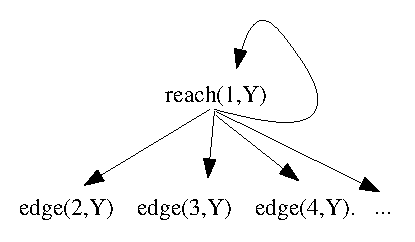
\includegraphics[width=\textwidth]{recursion}
%  \caption{Without \abstraction}
%  \label{fig:minipage1}
\end{minipage}
\quad
\begin{minipage}[b]{0.25\linewidth}
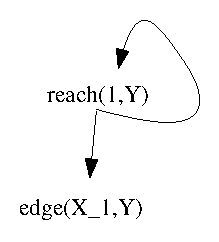
\includegraphics[width=0.5\textwidth]{abs-recursion}
%  \caption{With \abstraction}
%  \label{fig:minipage2}
\end{minipage}
\caption{A left-linear program and schematic IDGs: Left
  without IDG abstraction; Right: with
  IDG abstraction} \label{fig:abstraction}
\end{figure}
%------------------------------------------------------------
Abstracting the {\tt edge/2} predicate has subtle differences from
abstracting tabled subgoals.
%  The implementation of subgoal
%abstraction for tabled subgoals was described in~\cite{RigS13},
As mentioned, the {\tt edge/2} predicate of
Fig.~\ref{fig:abstraction} is not tabled.  Furthermore, the actual
{\tt edge/2} subgoal itself should not be abstracted to depth 0 since
losing the first argument instantiation would prevent the use of
indexing.  Rather, only the IDG's representation of the subgoal
should be abstracted.  Abstraction of dynamic code for
the IDG can be specified via the declaration:
\begin{center}
{\tt :-dynamic edge/2 as incremental, abstract(0)}.
\end{center}

In \version{} dynamic incremental code can be abstracted, but
incremental interned tries (Section~\ref{sec:incr-update-tries})
cannot be.  Also, currently only depth 0 abstraction is supported.

\subsection{Summary and Implementation Status}
%
%When using incremental tabling, an application will most commonly need
%only the default transparent approach, although in special
%circumstances eager updating may be desired.  

The main design choices of incremental tabling
are as usual what to table, and also what dynamic predicates or tries
should be made incremental.  In addition, performance optimizations
may be made through a mixture of subgoal abstraction and dynamic
predicate abstraction.  This optimization can be informed by use of
{\tt statistics/0} which includes summary information about the IDG,
or using the IDG inspection predicates of
Section~\ref{sec:incr-preds1} if more details are needed.

%Thus the user has four choices: tables may be
%updated as soon as the database is changed (e.g., via {\tt
%  incr\_assert/1}); at some point after a series of database changes
%(e.g. via {\tt incr\_assert\_inval/1} and {\tt
%  incr\_table\_update/0}); or lazily whenever a given table is called.
%In addition, if the changes are so massive that there is no point in
%incrementally updating the table, the tables can be abolished so that
%the tables will be reconstructed whenever they are re-queried.

In the current version of XSB, incremental tabling has not yet been
ported to the multi-threaded engine.  In addition, incremental tabling
only works for predicates that use both call and answer variance.
However, incremental tabling does work with for the full well-founded
semantics, for trie indexed dynamic code (in addition to regular
dynamic code) and with interned tries as described in
Section~\ref{sec:incr-update-tries}.  The space reclamation predicates
{\tt abolish\_all\_tables/0}, {\tt abolish\_table\_call/[1,2]} and
{\tt abolish\_table\_pred/[1,2]} can be safely used with incremental
tables.

\subsection{Predicates for Incremental Table Maintenance} \label{sec:incr-preds1}

\paragraph{A Note on Terminology}
%
Suppose {\tt p/1} and {\tt q/1} are incrementally tabled, and that
there is a clause
%
\begin{verbatim}
p(X):- q(X).
\end{verbatim}
%
In this case we say that {\tt p(X)} {\em depends\_on} {\tt q(X)} and
that {\tt q(X)} {\em affects} {\tt p(X)}.  A recursive predicate both
depends on and affects itself.


\paragraph{Declarations} The following directives support incremental
tabling based on changes in dynamic code: 

\index{tabling!opaque}
\index{tabling!declarations}
\begin{description}
\index{tabling!incremental}

\ourstandarditem{table +PredSpecs as incremental}{table/1}{Tabling}
%
is a executable predicate that indicates that each tabled predicate
specified in {\tt PredSpec} is to have its tables maintained
incrementally.  {\tt PredSpec} is a list of skeletons, i.e. open
terms, or {\tt Pred/Arity} specifications~\footnote{No explicit module
  references are allowed.}.  The tables must use call variance and
answer variance and must be compiled and loaded into the
single-threaded engine.  If a predicate is declared with tabling
attributes that are not supported with incremental tabling a
permission error is thrown.  This predicate implies that its arguments
are tabled predicates.  See page \pageref{table-declaration} for
further discussion of tabling options.

We also note that any tabled predicate that is called by a predicate
tabled as incremental must also be tabled as incremental or as opaque.
On the other hand, a dynamic predicate {\tt d/n} that is called by a
predicate tabled as incremental may or may not need to be declared as
incremental.  However if {\tt d/n} is not declared incremental, then
changes to it will not be propagated to incrementally maintained
tables.

\ourstandarditem{dynamic +PredSpecs as incremental}{dynamic/1}{Tabling}
%
is an executable predicate that indicates that each predicate in {\tt
  PredSpecs} is dynamic and used to define an incrementally tabled
predicate and will be updated using {\tt incr\_assert/1} and/or {\tt
  incr\_retractall/1} (or relatives.)  Note that dynamic incremental
predicates cannot themselves be tabled.  This predicate implies that
its arguments are dynamic predicates.  See page
\pageref{dynamic-declaration} for further discussion of dynamic
options.

\ourstandarditem{table +PredSpecs as opaque}{table/1}{Tabling} 
%
is an executable predicate that indicates that each predicate $P$ in
{\tt PredSpecs} is tabled and is used in the definition of some
incrementally tabled predicate but should not be maintained
incrementally.  In this case the system assumes that the programmer
will abolish tables for $P$ in such a way so that re-calling it will
always give semantically correct answers.  In other words, instead of
maintaining information to support incremental table maintenance, the
system re-calls the opaque predicate whenever its results are required
to recompute an answer.  One example of an appropriate use of opaque
is for tabled predicates in a DCG used to parse some string.  Rather
than incrementally maintain all dependencies on all input strings, the
user can declare these intermediate tables as opaque and abolish them
before any call to the DCG.  This predicate implies that its arguments
are tabled predicates.

\end{description}

\paragraph{Basic Incremental Maintenance Predicates}
The following predicates are used to manipulate incrementally
maintained tables:

\begin{description}
\ourrepeatmoditem{incr\_assert(+Clause)}{incr\_assert/1}{increval} 
\ourrepeatmoditem{incr\_assertz(+Clause)}{incr\_assertz/1}{increval}
\ourrepeatmoditem{incr\_asserta(+Clause)}{incr\_asserta/1}{increval}
\ourrepeatmoditem{incr\_retract(+Clause)}{incr\_retract/1}{increval}
\ourmoditem{incr\_retractall(+Term)}{incr\_retractall/1}{increval}
% 
are versions of {\tt assert/1} and other standard Prolog predicates.
They modify dynamic code just as their Prolog counterparts, but they
first invalidate all incrementally maintained tables that depend on
{\tt Clause}.

{\bf Error Cases} are the same as {\tt assert<a/z>/1}, {\tt retract/1}
and {\tt retractall/1} with the additional error conditions that
relate to the semantics of incremental tabling.  Note that if these
error conditions arise, the update will {\tt not} occur.

\begin{itemize}
\item The head of the clause {\tt Clause} or the {\tt Term} refers to
  a predicate that is not incremental and dynamic.  
\bi
\item  {\tt type error(dynamic\_incremental, Term)}
\ei
%
\item {\tt Clause} affects an incremental table that is incomplete
  (and so is in the course of being computed).
\bi
\item  {\tt permission\_error}
\ei 
\end{itemize}

%\ourrepeatmoditem{incr\_assert\_immed(+Clause)}{incr\_assert\_immed/1}{increval}
%\ourrepeatmoditem{incr\_assertz\_immed(+Clause)}{incr\_assertz\_immed/1}{increval}
%\ourrepeatmoditem{incr\_asserta\_immed(+Clause)}{incr\_asserta\_immed/1}{increval}\
%\ourrepeatmoditem{incr\_retractall\_immed(+Clause)}{incr\_retractall\_immed/1}{increval}
%\ourmoditem{incr\_retract\_immed(+Term)}{incr\_retract\_immed/1}{increval}
%%
%are versions of {\tt assert/1} and other standard Prolog predicates.
%They modify dynamic code just as their Prolog counterparts, mark any
%incrementally maintained tables that depend on the modification as
%invalid, then immediately update these tables.
%%  The tables may be updated by an
%explicit call to {\tt incr\_table\_immed/[0,1,2]}, or the table will
%be dynamically recomputed when a query is made to it.

%\ourmoditem{incr\_table\_update}{incr\_table\_update/0}{increval} may
%be called after base predicates have been changed (by {\tt
%  incr\_assert/1} and/or {\tt incr\_retract/1} or friends).  This
%predicate updates all the incrementally maintained tables whose
%contents may be affected by those changes to the base predicates.
%This update operation is separated from the operations that change the
%base predicates ({\tt incr\_assert\_inval/1} and {\tt
%  incr\_retractall\_inval/1}) so that a set of base predicate changes
%can be processed all at once, which may be much more efficient that
%updating the tables at every base update.  Beginning with Version
%3.3.7, it is not absolutely necessary to call this predicate, as
%tables will be incrementally updated upon demand.  However, using this
%predicate allows a choice of incurring the cost of update at a time
%other than querying an updated goal.
%Explicit update calls only need to be used in special circumstances
%(cf. Section~\ref{sec:incr-eager}).

%{\bf Error Cases}
%\bi
%\item A table $T$ that is to be incrementally updated is not yet
%  complete.  
%\bi
%\item 	{\tt permission\_error(update, incomplete\_table Goal)}
%\ei
%\item An abolish of some incremental table has made the global update
%  list potentially corrupted.
%\bi
%\item {\tt permission\_error}
%\ei 
%  \ei

%\ourmoditem{incr\_table\_update(-GoalList)}{incr\_table\_update/1}{increval}
%acts as {\tt incr\_table\_update/0} in its action to update the
%incrementally maintained tables after changes to base predicates.  It
%returns the list of goals whose tables were changed in the update
%process.
%
%\ourmoditem{incr\_table\_update(+SkelList,-GoalList)}{incr\_table\_update/2}{increval}
%acts as {\tt incr\_table\_update/1} in its action to update
%incrementally maintained tables after changes to base predicates.  The
%first argument is a list of predicate skeletons (open terms) for
%incrementally maintained tables.  The predicate returns in {\tt
%  GoalList} a list of goals whose skeletons appear in {\tt SkelList}
%and whose tables were changed in the update process.  In this way {\tt
%  SkelList} acts as a filter to restrict the goals that are returned
%to those of interest.  If {\tt SkelList} is a variable, all affected
%goals are returned in {\tt GoalList}.

\ourmoditem{incr\_invalidate\_call(+Goal)}{incr\_invalidate\_call/1}{increval}
Let $\cT$ be the least set of all incrementally maintained tables
whose goals that unify with {\tt Goal}, or whose tables are
(transitively) affected by a goal in $\cT$.  This predicate invalidates
all tables in $\cT$.  Any subsequent call to a goal $G$ associated
with $\cT$ will be automatically be incrementally updated if
necessary.  (As will any goals that $G$ depends on that are in need of
updating.)  In a similar manner, an invocation of {\tt
  incr\_table\_update/[0,1,2]} will cause tables in $\cT$ to be
updated.

Note that this predicate is needed for exceptional cases only.  Calls
to {\tt incr\_assert/1} and similar predicates mentioned above perform
invalidation automatically, as does {\tt abolish\_table\_call/[1,2]}.
However, {\tt incr\_invaldate\_calls/1} is useful if a tabled
predicate depends on some external data and not (only) on dynamic
incremental predicates.  For example, such a predicate might depend on
a relation stored in an external relational database (perhaps accessed
through the ODBC interface).
% then this predicate can be used to invalidate the
%table when the external relation changes.  
Of course, in such a case, the application programmer must know when
the external relation changes and invoke {\tt
  incr\_invalidate\_calls/1} as necessary.


{\bf Error Cases}
\bi
\item 	{\tt Goal} is tabled, but not incrementally tabled
\bi
\item 	{\tt permission\_error(invalidate,non-incremental predicate,Goal)}
\ei
\ei

\end{description}

\paragraph{Incremental Maintenance using Interned Tries}
The following predicates are used to modify incremental tries, and can
be freely intermixed with predicates for modifying incremental dynamic
code, as well as with predicates for invalidating or updating tables
(Section~\ref{sec:incr-preds1}).

\begin{description}
\ourmoditem{incr\_trie\_intern(+TrieIdOrAlias,+Term)}{incr\_trie\_intern/2}{intern}
%
is a version of {\tt trie\_intern/2} for tries declared as
incremental.  A call to this predicate interns {\tt Term} in {\tt
  TrieIdOrAlias} and then invalidates all incrementally maintained
tables that depend on this trie.

\ourmoditem{incr\_trie\_uninternall(+TrieIdOrAlias,+Term)}{incr\_trie\_uninternall/2}{intern}
%
is a version of {\tt trie\_unintern/2} for tries declared as
incremental.  A call to this predicate removes all terms unifying with
{\tt Term} in {\tt TrieIdOrAlias} and then invalidates all
incrementally maintained tables that depend on this trie.

%\ourmoditem{incr\_trie\_intern\_immed(+TrieIdOrAlias,+Term)}
%           {incr\_trie\_intern\_immed/2}{intern}
%%
%works for tries declared as incremental in a similar manner as {\tt
%  incr\_trie\_intern/2} except that it also immediatesly updates any
%affected tables.

%\ourmoditem{incr\_trie\_uninternall\_immed(+TrieIdOrAlias,+Term)}
%{incr\_trie\_uninternall\_immed/2}{intern}
%
%works for tries declared as incremental in a similar manner as {\tt
%  incr\_trie\_uninternall/2} except that it also immediately updates
%any affected tables.
\end{description}

\index{residual dependency graph}
\index{Incremental Dependency Graph (IDG)}
\paragraph{Inspecting the State of the Incremental Dependency Graph}
%
% These relations form a labelled directed graph for which the
%nodes are incrementally tabled subgoals present in XSB; a given
%subgoal in the graph may or may not have been completed.  
%Conceptually, there is an edge from $S_1$ to $S_2$ labelled depends
%(affects) if $S_1$ directly depends on (directly affects) $S_2$.  We
%call this graph the {\em incrementally tabled subgoal dependency
%  graph}, or just the incremental dependency graph.  
The predicates in this section allow a user to inspect properties of
IDG that can be useful in debugging, profiling or optimizing a
computation~\footnote{The predicates for traversing the incremental
  dependency graph are somewhat analogous to those for traversing the
  residual dependency graph (Section~\ref{sec:table-inspection}).}.
In addition they provide information about which subgoals in the IDG
are invalid -- i.e., which subgoals depend on a dynamic code that has
changed, but have not been updated.

As explained below, IDG nodes can be accessed via the predicate {\tt
  is\_incremental\_subgoal/1}, while IDG edges can be accessed via
{\tt incr\_directly\_depends/2}.  The predicates {\tt
  get\_incr\_scc/[1,2]} and {\tt get\_incr\_scc\_with\_deps/[3,4]} can
be used to efficiently materialize the dependency graph in Prolog,
including SCC information.  Similarly, the predicate {\tt
  subgoal\_property/2} can be used to determine which subgoals are
invalid.

\begin{description}

\ourmoditem{is\_incremental\_subgoal(?Subgoal)}{is\_incremental\_subgoal/1}{increval}
%
This predicate non-deterministically unifies {\tt Subgoal} with
incrementally tabled subgoals that are currently table entries.

\ourmoditem{incr\_directly\_depends(?Goal$_1$,?Goal$_2$)}{incr\_directly\_depends/2}{increval}
accesses the edges of the IDG: the incremental goals (Tables) that
directly depend on or directly affect one another.  At least one of
{\tt Goal$_1$} or {\tt Goal$_2$} must be bound.
\begin{itemize}
\item If {\tt Goal$_1$} is bound, then this predicate will return in
  {\tt Goal$_2$} through backtracking the goals for all incrementally
  maintained tables and dynamic leaf nodes on which {\tt Goal$_1$}
  directly depends.
\item If {\tt Goal$_2$} is bound, then it returns in {\tt Goal$_1$}
  through backtracking the goals for all incrementally maintained
  tables that {\tt Goal$_2$} directly affects -- in other words all
  goals that directly depend on {\tt Goal$_2$}.  \ei

{\bf Error Cases}
\bi
\item Neither {\tt Goal$_1$} nor {\tt Goal$_2$} is bound 
\bi
\item 	{\tt instatiation\_error}
\ei
\item {\tt Goal$_1$} and/or {\tt Goal$_2$} is bound, but is not
  incrementally tabled
\bi
\item 	{\tt table\_error}
\ei
\ei

\ourmoditem{incr\_trans\_depends(?Goal$_1$,?Goal$_2$)}{incr\_trans\_depends/2}{increval}
is similar to {\tt incr\_directly\_depends/2} except that it returns
goals according to the transitive closure of the ``directly depends''
Xrelation.  Error conditions are the same as {\tt
  incr\_directly\_depends/2}.

\ourmoditem{add\_incr\_dependency(Goal)}{add\_incr\_dependency/1}{increval}
%
Incremental tabling creates dependency graphs dynamically, so that
specific goal bindings can always be used.  This works well the great
majority of the time, but consider the following case:
\begin{verbatim}
:- dynamic p/1, q/2 as incremental.
:- table t1/2 as incremental.
t1(X,1):- p(X,Y),!.
t1(X,Y):- q(X,Y).

p(1,2).
\end{verbatim}
In the case of the goal {\tt ?- t1(1,Y)} the first clause will
succeed, cutting away the second clause so that the dependency of {\tt
  t1(1,Y)} on {\tt q(1,Y)} is never added, which may cause unexpected
behavior later in execution if new clauses are added or retracted for
{\tt q/1}.  Such a situation can be addressed using {\tt
  add\_inc\_dependency/2} by rewriting {\tt t1/2} as:
\begin{verbatim}
t1(X,Y):- p(X,Y),!,add_incr_dependency(q(X,Y)).
t1(X,Y):- q(X,Y).
\end{verbatim}
It must be stressed, however, that it should not be common to need {\tt
  add\_incr\_dependency/1} and it should be avoided in most (though not all) situations.

\ourrepeatmoditem{get\_incr\_sccs(?SCCList)}{get\_incr\_sccs/1}{increval}
\ourrepeatmoditem{get\_incr\_sccs\_with\_deps(?SCCList,?DepList)}{get\_incr\_sccs\_with\_deps/2}{increval}
\ourrepeatmoditem{get\_incr\_sccs(+SubgoalList,?SCCList)}{get\_incr\_sccs/2}{increval}
\ourmoditem{get\_incr\_sccs\_with\_deps(+SubgoalList,?SCCList,?DepList)}{get\_incr\_sccs\_with\_deps/3}{increval}
%

%{\bf {\em Warning: these predicates may be obsolescent, cf.
%    Section~\ref{sec:dep-graph} for newer predicates that are more
%    powerful.}}
%
%Most linear algorithms for SCC detection over a graph use destructive
%assignment on a stack to maintain information about the connectedness
%of a component; as a result such algorithms are
%difficult to write efficiently in Prolog.
%
%{\tt get\_incr\_sccs/1} unifies {\tt SCCList} with SCC information for
%the incremental dependency graph that is represented as a list whose
%elements are of the form
%\begin{center}
%{\tt ret(Subgoal,SCC)}.
%\end{center}
%{\tt SCC} is a numerical index for the SCCs of Subgoal. Two subgoals
%are in the same SCC iff they have the same index, however no other
%dependency information can be otherwise directly inferred from the
%index~\footnote{The actual number for each SCC index depends on how
%  the incremental dependency graph happens to be traversed; as a
%  result it is best to rely on the index only as a ``generated'' name
%  for each SCC.}.
%
%If dependency information is also desired, {\tt
%  get\_incr\_scc\_with\_dependencies/2} should be called.  In addition
%to the SCC information as above, {\tt DepList} is unified with a list
%of dependency terms of the form
%\begin{center}
%{\tt depends(SCC1,SCC2)}
%\end{center}
%for each pair {\tt SCC1} and {\tt SCC1} such that some subgoal with
%index {\tt SCC1} directly depends on some subgoal with index {\tt
%  SCC1}.  If it is necessary to know which subgoal(s) in {\tt SCC1}
%directly depends on which subgoal(s) in {\tt SCC2}, the information
%can be easily reconstructed using {\tt incr\_directly\_depends/2}
%above.  Similarly, {\tt incr\_directly\_depends/2} can be used to
%determine the actual edges within a given SCC.
%
%Ordinarily a user will want to see the entire dependency graph and in
%such a case the predicates described above should be used.  However,
%note that if the dependency graph is the result of several
%independent queries it may not be connected.  {\tt get\_incr\_scc/2}
%takes as input a list of incremental subgoals, {\tt SubgoalList}.  For
%each {\tt Subgoal} in {\tt SubgoalList}, this predicate finds the set
%of subgoals connected to {\tt Subgoal} by any mixture of depends and
%affects relations, unions these sets together, and finds the SCCs of
%all subgoals in the unioned set.
%
%SCC detection is implemented using Tarjan's algorithm~\cite{Tarj72} in
%C working directly on XSB's data structures.  The algorithm is
%\cO(|V| + |E|)$ where $|V|$ is the number of vertices and $|E|$ the
%number of edges in the dependency graph.  As a result, {\tt
%  get\_incr\_sccs/[1,2]} provides an efficient means to materialize the
%  high-level topography of the dependency graph~\footnote{Currently,
%    the materialization of dependency information between SCCs is
%    implemented in a naive manner, so that {\tt
%      get\_incr\_sccs\_with\_deps/[2,3]} is $\cO(|V|^2)$.}.%%%
%
%{\bf Error Cases}
%\bi
%\item {\tt SubgoalList} is a variable
%\bi
%\item 	{\tt instantiation\_error}
%\ei
%\item {\tt SubgoalList} is not a list
%\bi
%\item 	{\tt type\_error}%
%\ei
%\item {\tt SubgoalList} contains a predicate that is not tabled
%\bi
%\item 	{\tt permission\_error}
%\ei%
%\ei
%}
%\ourmoditem{incr\_invalid\_subgoals(-List)}{incr\_invalid\_subgoals/1}{increval}
%
%This predicate unifies {\tt List} with a sorted list of the
%incremental subgoals that are currently invalid.

%\ourmoditem{incr\_is\_invalid(+Subgoal)}{incr\_is\_invalid/1}{increval}
%
%Succeeds if {\tt Subgoal} is an incrementally tabled subgoal that is
%invalid, and fails otherwise.

\end{description}


%--------------------------------------------------------------------

\section{A Weaker Semantics for Tabling}
%
\index{completion semantics}
\index{completion semantics!weak}
Recall that the well-founded semantics (WFS) is weaker than, say,
the Stable model semantics.  For instance a program like
%
\begin{verbatim}
p:- not q.            q:- not p.
\end{verbatim}
%
has two stable models: $\{p\}$ and $\{q\}$.  On the other hand, WFS
has a single model, where both $p$ and $q$ are undefined.  This, of
course, is characteristic of the way WFS treats atoms whose only
non-failed derivations are based on a ``negative loop''.

However, an even weaker logic is possible where derivations based on
positive loops are also considered undefined.  In other words the
program
\begin{verbatim}
   r:- r.                r:- false.
\end{verbatim}
would assign the truth value {\em undefined} to $r$, although both WFS
and stable models would assign r as {\em false}.  But why use such a
weak logic?

Consider a woman who asks her husband when he'll clean the garage, and
the husband says:

{\em I'll get around to it when I get around to it.}

The wife would probably consider it ambiguous not only when her
husband might clean the garage, but whether he would do so at all.
The wife's reasoning (slightly simplified) could be rendered in logic
as:

\begin{verbatim}
   clean_the_garage:- clean the garage.
\end{verbatim}
\noindent
and we'd like to assign {\em undefined} or {\em unknown} to {\tt
  clean\_the\_garage}.\footnote{Actually, many wives would go ahead
  and assign {\em false} to this statement, but we are modeling an
  optimistic (or possibly delusional) wife.}

Although this example is somewhat fanciful, it turns out that this
interpretation accords with the results of cognitive science
experiments about human reasoning~\cite{SteV08}, and is known in the
logic programming community as the ``completion semantics'' (CS).  CS
differs from WFS only in assigning the truth value {\em undefined} to
derivations that depend on a positive loop, and that are otherwise not
satisfiable (cf. \cite{Lloy84}).

%Thus, in this
%new semantics positive loops are treated in an analogous way to
%negative loops.Formally, the new semantics can be expressed as a fixed
%point logic based on Clark's completion semantics~\cite{??}, when
%logical expressions are satisfied according to the Lukasiewicz
%3-valued semantics for propositional programs, which is weaker than
%some other approaches to 3-valued satisfiability, namely that of
%Kleene (see \cite{??}).  However, this level of formality is not
%necessary as long as one understands how positive and negative loops
%are evaluated.  We call this semantics the {\em completion semantics
%  (CS)}.

So as useful as WFS and stable models are for programming, they don't
reflect how human beings have been shown to reason in daily life.
However, there is another difference between WFS and the sort of
common-sense reasoning that humans perform.  WFS has a strong {\em
  closed-world} assumption.  Suppose a query {\tt ?- s} were made to a
program where {\tt s} were not defined.  WFS would assign the value
{\em false} to {\tt s}, but this is not always what humans do: rather
humans would treat the unknown predicate {\tt s} as in fact {\em
  unknown} or {\em undefined}.  More generally, if (sub-)goal $G$
refers to an undefined predicate,the {\em weak} completion semantics
(WCS) also assigns {\em undefined} to $G$, rather than {\em false} as
WFS does, or throwing an error (as XSB also does by default).

\begin{itemize}
\item For one or more tabled predicates ro use the completion semantics,
use the declaration

\noindent
{\tt \mif{} table {\em PredSpec} as compl\_semantics.}

\item Setting the ISO Prolog flag {\tt unknown} to {\tt undefined}
  makes calls to unknown predicates return the truth value {\em
    undefined}.  E.g., 
\begin{verbatim}
?- set_prolog_flag(unknown,undefined).
\end{verbatim}
This flag can also be set to the standard ISO values,
  {\tt fail}. {\tt warning} or {\tt error} (the last of which is the
    default).

\item The various forms of tabled negation work well with the
  completion semantics; however if mixing tabled and non-tabled
  predicates it is best to use {\tt not3/1} (cf. pg. \pageref{not3})
  rather than the SLD operators {\tt not/1} or \verb|\+/1|.
\end{itemize}

%\noindent
%These features can be set globally either separately or together:

%\begin{itemize}
%\item \item Setting the Prolog flag {\tt alt\_semantics} to {\tt cs} causes
%  XSB to globally evaluate the completion semantics.
%\item Setting the Prolog flag {\tt alt\_semantics} to {\tt weak\_cs} causes
%  XSB to globally evaluate the weak completion semantics, and is
%  equivalent to setting the {\tt alt\_semantics} flag to {\tt cs} and
%  the ISO flag {\tt unknown} to {\tt undefined}.
%\item Setting the Prolog flag {\tt alt\_semantics} to {\tt wfs} turns
%  causes XSB to behave in its default mode.  I.e., to globally
%  evaluate queries according to the well-founded semantics, and to
%  throw an error when encountering an unknown predicate.
%\end{itemize}

(W)CS and WFS can be mixed on a per-predicate basis.  If a goal
$G_{WFS}$ to a predicate declared to use WFS is involved in a loop
with a goal $G_{CS}$ declared to use CS, then $G_{WFS}$ is evaluated
according to the (W)CS.

\paragraph{Examples}

As a simple example, consider the program:
\begin{verbatim}
:- table simple_loop/1 as compl_semantics.
simple_loop(X):- simple_loop(X).     simple_loop(X):- p(X).
p(a).
\end{verbatim}
The query {\tt ?- simple\_loop(X)} returns two answers: {\tt X = a} as
{\em true}, and {\tt X} unbound as {\em undefined}.

For a more complex example, consider the program:
\begin{verbatim}
:- table m_1_1/1,m_1_2/1,m_1_3/1,m_1_4/1 as compl_semantics.
m_1_1(X):- m_1_2(X).         m_1_1(a):- m_1_2(a).
m_1_2(X):- m_1_3(X).         m_1_2(a):- m_1_3(a).         
m_1_3(X):- m_1_4(X),fail.    m_1_3(a):- m_1_4(a).
m_1_4(X):- m_1_1(X).         m_1_4(a):- m_1_1(a).
\end{verbatim}
%
The derivation of the query {\tt ?- m\_1\_1(X)} creates a positive SCC
with with numerous interrelated positive cycles, but these cycles can
be broken down into two groups.  The first group includes a dependency
edge from {\tt m\_1\_3(X)} to {\tt m\_1\_4(X)}, while the other set
does not include this edge.  Due to the first clause of {\tt
  m\_1\_3(X)}, all derivations in the first group fails, although
derivations that do not include this edge succeed.  Thus the only
answer to {\tt m\_1\_1(X)} has {\tt X = a} with truth value {\em
  undefined} (and a single delay list of {\tt [m\_1\_2(a)]}.


\index{tabling!call subsumption}
\index{tabling!call variance}
\index{tabling!answer subsumption}
\index{tabling!incremental}

\section{Compatibility of Tabling Modes and Predicate Attributes} \label{sec:tabling-compatibility}
%
As discussed in this chapter, there are numerous choices for how to
table a predicate. Either call subsumption or call variance may be
used, incremental tabling might or might not be used, and answer
subsumption might or might not be used.  Ground terms may be interned.
Furthermore, a tabled predicate, like any other predicate, may be
static or dynamic.
%and thread-shared or thread-private.
Additionally various abstraction methods may be used, such as subgoal
abstraction, answer abstraction, or maximal answers.
%And finally, a
%tabled predicate may be declared as private or shared in the
%multi-threaded engine.

To analyze further, all combinations are supported for call-variance
except for table indexing, which is a means of optimizing call
subsumption (cf. Section~\ref{sec:table-index}).
%and for thread-private predicates.
However, call subsumption has not been fully integrated with dynamic
code,
%or thread-shared predicates,
and cannot currently be combined
%with incremental tabling or
with answer subusmption.
%Similarly incremental tabling is not yet supported
%in the multi-threaded engine (it is supported for ``thread-private''
%computations only in the sequential engine).
All compatibilities are listed below: further combinations will be
supported in future versions of XSB as resources allow.

%The combinations in Table~\ref{table:table} allow full well-founded
%computation, constrained variables in calls and answers (including the
%residual program), and safe space reclamation, with the following
%exceptions.  Answer subsumption does support non lrd-stratified
%programs; and call subsumption does not yet support attributed
%variables in calls.  \index{attributed variables}

\begin{itemize}
\item A predicate $P$ declared with {\tt ans\_subsumption} cannot also
  be declared with {\tt answer\_abstract, compl\_semantics, dynamic,
    incremental, index/1, intern, opaque, subgoal\_abstract} or {\tt
    subsumptive}.
%
\item A predicate $P$ declared with {\tt answer\_abstract} cannot also
  be declared with {\tt ans\_subsumption, compl\_semantics, intern} or
  {\tt subsumptive}.
%
\item A predicate $P$ declared with {\tt compl\_semantics} cannot also
  be declared with {\tt ans\_subsumption, answer\_abstract, dynamic,
    incremental, index/1, intern, opaque, subsumptive} or {\tt subgoal\_abstract}.
%
\item A predicate $P$ declared with {\tt dyn} or {\tt (dynamic)}
  cannot also be declared with {\tt ans\_subsumption}, {\tt
    incremental} or {\tt subsumptive}.
%
\item A predicate $P$ declared with {\tt incremental} cannot also be
  declared with {\tt compl\_semantics, dynamic, index/1, intern,
    nonincremental} or {\tt opaque}.
  %, shared} or {\tt subsumptive}.
  However, $P$ may be changed from {\tt incremental} to {\tt
    nonincremental} or {\tt opaque} via {\tt
    set\_predicate\_property/2}.
%
\item A predicate $P$ declared with {\tt index/1} cannot also be
  declared with any option that is incompatible with {\tt subsumptive}
  since table indexing is a form of call subsumption.
%
\item A predicate $P$ declared with {\tt intern} cannot also be
  declared with {\tt ans\_subsumption, answer\_abstract,
    compl\_semantics, incremental, index/1, subgoal\_abstract} or {\tt
    subsumption}
%
\item A predicate $P$ declared with {\tt max\_answers} cannot also be
  declared with {\tt compl\_semantics, index/1} or {\tt subsumptive}.
%
\item A predicate $P$ declared with {\tt nonincremental} cannot also
  be declared with {\tt incremental} or {\tt opaque}.  However, $P$
  may be changed from {\tt nonincremental} to {\tt incremental} or
  {\tt opaque} via {\tt set\_predicate\_property/2}.
%
\item A predicate $P$ declared with {\tt opaque} cannot also be
  declared with {\tt incremental} or {\tt nonincremental}.  However,
  $P$ may be changed from {\tt opaque} to {\tt nonincremental} or {\tt
    incremental} via {\tt set\_predicate\_property/2}.
%
%\item A predicate $P$ declared with {\tt private} cannot also
%  be declared with {\tt shared}.
%
%\item A predicate $P$ declared with {\tt shared} cannot also be
%  declared with {\tt compl\_semantics, incremental, opaque, private}
%  or {\tt subsumptive}.
%
\item A predicate $P$ declared with {\tt subgoal\_abstract} cannot also
  be declared with {\tt index/1} or {\tt subsumptive}.
%
\item A predicate $P$ declared with {\tt subsumptive} cannot also be
  declared with {\tt compl\_semantics, dynamic, max\_answers}
%, shared}
    or {\tt subgoal\_abstract}.  However, $P$ may be changed from {\tt
      subsumptive} to {\tt variant} via {\tt
      set\_predicate\_property/2}.
%
\item A predicate $P$ declared with {\tt variant} cannot also be
  declared with {\tt index/1} or {\tt subsumptive}. However, $P$ may be changed from
  {\tt variant} to {\tt subsumptive} via {\tt
    set\_predicate\_property/2}.

\end{itemize}

%\begin{table}
%\begin{center}
%{\footnotesize
%\begin{tabular}{llllll}\hline \hline
%%variant/subsumptive & dynamic/static & shared/private & incremental/opaque  & answer subsumption  \\
%variant &	    static & 	   private &	  nonincremental &      no answer subsumption  &  yes \\
%%variant &	    static &	   private &	  nonincremental &      answer subsumption     &  yes \\
%variant	&	    static &	   private &      opaque &             no answer subsumption  &  yes \\
%variant &	    static &	   private &	  opaque &	      answer subsumption &	no \\
%variant &	    static &	   private &	  incremental &         no answer subsumption &	yes \\
%variant &	    static &	   private &      incremental &         answer subsumption &	no \\
%variant &	    static &	   shared &	  nonincremental &      no answer subsumption &	yes \\
%variant &	    static &	   shared &	  nonincremental &      answer subsumption &	yes \\
%variant &	    static &	   shared &	  opaque &	      no answer subsumption &	no \\
%variant &	    static &	   shared &	  opaque &	      answer subsumption &	no \\
%variant &	    static &	   shared &	  incremental &       no answer subsumption &	no \\
%variant &	    static &	   shared &	  incremental &          answer subsumption &	no \\
%variant &	    dynamic &	   private &	  nonincremental &      no answer subsumption &	yes \\
%ariant &	    dynamic &	   private &	  nonincremental &      answer subsumption &	yes \\
%variant &	    dynamic &	   private &	  opaque &	      no answer subsumption &	no \\
%variant &	    dynamic &	   private &	  opaque &	      answer subsumption &	no \\
%variant &	    dynamic &	   private &	  incremental &         no answer subsumption &	no \\
%%variant &	    dynamic &	   private &	  incremental &         answer subsumption &	no \\
%variant &	    dynamic &	   shared &	  nonincremental &      no answer subsumption &	yes \\
%variant &	    dynamic &	   shared &	  nonincremental &      answer subsumption &	yes \\
%variant &	    dynamic &	   shared &	  opaque &	      no answer subsumption &	no \\
%variant &	    dynamic &	   shared &	  opaque &	      answer subsumption &	no \\
%variant &	    dynamic &	   shared &	  incremental &         no answer subsumption &	no \\
%variant &	    dynamic &	   shared &	  incremental &         answer subsumption &	no \\
%subsumptive &	    static &	   private &	  nonincremental &      no answer subsumption &	yes \\
%subsumptive &	    static &	   private &	  nonincremental &      answer subsumption &	yes \\
%subsumptive &	    static &	   private &	  opaque &	      no answer subsumption &	no \\
%subsumptive &	    static &	   private &	  opaque &	      answer subsumption &	no \\
%subsumptive &	    static &	   private &	  incremental &         no answer subsumption &	no \\
%subsumptive &	    static &	   private &	  incremental &         answer subsumption &	no \\
%subsumptive &	    static &	   shared &	  nonincremental &      no answer subsumption &	no \\
%subsumptive &	    static &	   shared &	  nonincremental &      answer subsumption &	no \\
%subsumptive &	    static &	   shared &	  opaque &	      no answer subsumption &	no \\
%subsumptive &	    static &	   shared &	  opaque &	      answer subsumption &	no \\
%subsumptive &	    static &	   shared &	  incremental &       no answer subsumption &	no \\
%subsumptive &	    static &	   shared &	  incremental &          answer subsumption &	no \\
%subsumptive &	    dynamic &	   private &	  nonincremental &      no answer subsumption &	yes \\
%subsumptive &	    dynamic &	   private &	  nonincremental &      answer subsumption &	yes \\
%subsumptive &	    dynamic &	   private &	  opaque &	      no answer subsumption &	no \\
%subsumptive &	    dynamic &	   private &	  opaque &	      answer subsumption &	no \\
%subsumptive &	    dynamic &	   private &	  incremental &         no answer subsumption &	no \\
%subsumptive &	    dynamic &	   private &   	  incremental &         answer subsumption &	no \\
%subsumptive &	    dynamic &	   shared &	  nonincremental &      no answer subsumption &	no \\
%subsumptive &	    dynamic &	   shared &	  nonincremental &      answer subsumption &	no \\
%subsumptive &	    dynamic &	   shared &	  opaque &	      no answer subsumption &	no \\
%subsumptive &	    dynamic &	   shared &	  opaque &	      answer subsumption &	no \\
%subsumptive &	    dynamic &	   shared &	  incremental &         no answer subsumption &	no \\
%subsumptive &  	    dynamic &	   shared &	  incremental &         answer subsumption &	no \\ \hline \hline 
%\end{tabular}
%}
%\end{center}
%\caption{Support for different tabling modes in XSB \version}
%\label{table:table}
%\end{table}


%\section{Incremental Table Maintenance} \label{sec:incremental_tabling}
%====================================================

\index{tabling!incremental}

XSB allows the user to declare that the system should maintain the
correctness of a given table with respect to dynamically changing
facts and rules through so-called {\em incremental
  tables}~\cite{SaRa05,Saha06,Swif14}.
%A table $T$ is {\em incremental} if XSB ensures that its answers are
%  consistent with all dynamic facts and rules upon which $T$ depends
%  (subject to transactionality conditions explained below).
After a database update or series of updates $\Delta$, an incremental
table $T$ that depends on $\Delta$ is by default updated
transparently: that is $T$ and all tables upon which $T$ depends are
automatically updated (if needed) whenever a future subgoal calls $T$.
%Alternately, if circumstances require it, a table can be updated
%immediately upon a database change or by issuing an explicit command
%to update all tables that depend on $\Delta$.
%
In either case, incremental tabling brings XSB closer to the
functionality of deductive databases.  If tables are thought of as
materialized database views (or snapshots), then the incremental table
maintenance subsystem enables incremental view maintenance; also as
discussed below, if choice points are thought of as database cursors
then incremental tabling also provides view consistency~\footnote{In
  the current version of XSB, there are certain restrictions on how
  incremental tabling can be used:
  cf. Section~\ref{sec:tabling-compatibility}.}.

\subsection{Transparent Incremental Tabling} \label{sec:incr_examples}

To demonstrate incremental table maintenance (informally called {\em
  incremental tabling}), consider first the following simple program
that does not use incremental tabling:
\begin{verbatim}
:- table p/2.
p(X,Y) :- q(X,Y),Y =< 5.

:- dynamic q/2.
q(a,1).    q(b,3).   q(c,5).    q(d,7).
\end{verbatim}
and the following queries and results:
\begin{verbatim}
| ?- p(X,Y),writeln([X,Y]),fail.
[c,5]
[b,3]
[a,1]

no
| ?- assert(q(d,4)).

yes
| ?- p(X,Y),writeln([X,Y]),fail.
[c,5]
[b,3]
[a,1]

no
\end{verbatim}
%
In this program, the table for {\tt p/2} depends on the contents of
the dynamic predicate {\tt q/2}.  We first evaluate a query, {\tt
  p(X,Y)}, which creates a table.  Then we use {\tt assert/1} to add a
fact to the {\tt q/2} predicate and re-evaluate the query.  We see
that the answers haven't changed, because the table is already created
and the second query just retrieves answers directly from that
existing table.  However the answers are inconsistent with the model
of {\tt p/2} after the assert.  I.e., if the table didn't exist
(e.g. if {\tt p/2} weren't tabled), the answer {\tt [d,4]} would also
be derived.  Without incremental table maintenance, the only solution
to this problem is for the XSB programmer to explicitly abolish a
table whenever changing (with assert or retract) a predicate on which
the table depends.
%
By declaring that the tables for {\tt p/2} should be incrementally
maintained, XSB automatically keeps the tables for {\tt p/2} correct.

%
Consider a slight rewrite of the above program:
\begin{verbatim}
:- table p/2 as incremental.
p(X,Y) :- q(X,Y),Y =< 5.

:- dynamic q/2 as incremental.
q(a,1).    q(b,3).    q(c,5).     q(d,7).
\end{verbatim}
in which {\tt p/2} is declared to be incrementally tabled
% (with {\tt  :- table p/2 as incremental}) 
and {\tt q/2} is declared to be both dynamic and incremental, meaning
that an incremental table depends on it.
%~\footnote{The declarations {\tt use\_incremental\_tabling/1} and
%  {\tt use\_incremental\_dynamic/1} are deprecated from Version 3.3 of
%  XSB forward -- in other words backwards compatibility will be
%  maintained for a time, but these declarations will not be further
%  supported.}.  
Consider the following goals and execution:
\begin{verbatim}
| ?- import incr_assert/1 from increval.
yes
| ?- p(X,Y),writeln([X,Y]),fail.
[c,5]
[b,3]
[a,1]

no
| ?- incr_assert(q(d,4)).

yes
| ?- p(X,Y),writeln([X,Y]),fail.
[d,4]
[c,5]
[b,3]
[a,1]

no
\end{verbatim}
\noindent
\index{Incremental Dependency Graph (IDG)}
\index{tabling!incremental!invalid subgoals}
The transparent approach to incremental updating works as follows.
When {\tt incr\_assert/1} is called, it sparks an invalidation
phase in which tables that depend on {\tt q(d,4)} are marked as {\em
  invalid} (i.e., possibly inconsistent with respect to underlying
dynamic code).  An {\em Incremental Dependency Graph (IDG)} is used to
obtain the right tables to invalidate.  However, if the invalidation
phase finds an affected table that is incomplete, a permission error
is thrown, since it is unclear whether sensible semantics can be given
to updating a subgoal that is incomplete.  After the invalidation
phase is completed, when/if a subgoal calls an invalid table $T$ the
engine interrupts itself to recompute $T$ and any tables upon which
$T$ depends.  On the other hand, if no calls are ever made to an
invalid incremental table $T'$, $T'$ will never incur the cost of an
update.

\index{view consistency}
\subsubsection{View Consistency} \label{sec:view-consistency}
%
As described above, transparent incremental tablings's use of lazy
updating ensures that a new query $Q$ will always be consistent with
the state of the dynamic code at the time $Q$ is called.  However,
transparent incremental tabling enforces a stronger property of view
consistency similar to those of database systems: that answers to a
query $Q$ should be those derivable at the time $Q$ was called, {\em
  and should not be affected by any updates}.
%Accordingly, the ISO standard for Prolog~\cite{ISO-Prolog} specifies
%that an update $\upsilon$ to dynamic code should not affect the
%behavior of choice points that were created before $\upsilon$.
Because XSB's incremental tabling does not allow updates that affect
tables that are still being computed, supporting view consistency
effectively means ensuring consistency for choice points into
completed incremental tables.  As such choice points correspond to
database cursors, we term them {\em Open Cursor Choice Points,
  (OCCPs)}.

XSB's support for view consistency is designed so that no perceptible
overhead in incurred if there are no OCCPs whose view needs to be
maintained.  Not surprisingly, numerous long-lived OCCPs whose views
need to be maintained across updates causes an overhead for the
engine, a situation that is in some sense similar to the cost of
maintaining views for cursors in database system.

%----------------------------------------------------------------
\comment{
In addition to the success continuations that are standard in most
languages, Prolog has failure continuations -- choice points to take
upon backtracking.  The presence of these failure continuations leads
to an issue of view consistency, even within a single-threaded
computation.  Suppose that a user
%
\begin{enumerate}
\item Makes a query to a completed incrementally tabled subgoal $Q$.
  $Q$ has more than one solution and the first one is returned,
  leaving a choice point into the table for $Q$.
\item Makes an update to dynamic code upon which $Q$ depends
\item Makes another query to $Q$
\end{enumerate}
%
What is the relation between the queries and the update.  Presumably,
the first query in step 1) should not reflect the changes made in step
2) if a user backtracks for further answers to that query -- this can
be seen as ensuring view consistency.. However it is less clear
whether the second query to $Q$ in step 4) should return the same
answers as the first query in step 1), or whether the second query
should reflect the database update.  Arguments can be made for either
approach.
%
\begin{itemize}
\item {\em Prolog-style semantics} If the second query reflects the
  database change, it is consistent with the database, but is not
  consistent with the first query~\footnote{This approach could be
    viewed as an extension of the ISO semantics for dynamic code in
    Prolog, which XSB does not currently support.};
\item {\em Delayed update semantics} If the second query does not
  reflect the dynamic code change, it is consistent with the first
  query but not with the dynamic code change.
\end{itemize}
%
XSB chooses the latter of these approaches.  If a user has failure
continuations into a query $Q$, then $Q$ and all tables that depend on
$Q$ will not be updated until these failure continuations have been
exhausted or removed.  However, all updates are ensured to be applied
once this is the failure continuations are removed.
}

%----------------------------------------------------------------

\subsection{Updating in a Three-Valued Logic}
%
As discussed earlier in this chapter, answers that are undefined in
the well-founded semantics are represented as conditional answers.
Beginning with version 3.3.7, incremental updates work correctly with
conditional answers~\footnote{Before Version 3.3.7, incremental
  updates only worked correctly on stratified tables: those with only
  unconditional answers.}.  Nno special care needs to be taken for
updating in the well-founded semantics as the following example
illustrates.
%conditional answers, and they can be updated through any of the
%previously described methods.  The following example illustrates one
%such approach.

\begin{verbatim}
:- dynamic data/1 as incremental.

:- table opaque_undef/0 as opaque.
opaque_undef:- tnot(opaque_undef).

:- table p/1 as incremental.
p(_X):- opaque_undef.
p(X):- data(X).
\end{verbatim}
%
Note that {\tt opaque\_undef/1} upon which {\tt p/1} depends is
explicitly declared as opaque~\footnote{An {\em opaque} predicate $P$
  is tabled and is used in the definition of some incrementally tabled
  predicate but should not be maintained incrementally.  In this case
  the system assumes that the programmer will abolish tables for $P$
  in such a way so that re-calling it will always give semantically
  correct answers.}.  When the above program is loaded, XSB will
behave as follows.
%
{\small
\begin{verbatim}
| ?- p1(1).

undefined
| ?- incr_assert(data(1)).

yes
| ?- p1(1).

yes
| ?- incr_retract(data(1)).

yes
| ?- p1(1).

undefined
| ?- get_residual(p1(1),C).

C = [opaque_undef]
\end{verbatim}
}
%

%\subsection{Eager Incremental Tabling}~\label{sec:incr-eager}
%%
%Despite the advantages of transparent incremental tabling, there are
%special circumstances when it may be better to update tables eagerly
%rather than when (and if) they are called.  For instance, if updates
%and queries are expected to occur at different times, performing eager
%updates may improve query time.  In addition, if incremental tables
%are accessed via table inspection predicates
%(cf. Chapter~\ref{sec:TablingPredicates}) rather than by queries,
%inconsistent answers may be obtained.  
%
%\paragraph{An Eager Updating Approach}
%%
%Usually, best way to eagerly update tables is to use the {\tt
%  incr\_assert/1} and {\tt incr\_retract(all)/1}
%predicates as discussed above.  When the updates are finished, the
%ommand {\tt incr\_table\_update/0} is then called, which updates all
%tables that depend on any changed dynamic rules or facts.  The
%following execution for our running program shows an example of this.

%\begin{verbatim}
%| ?- import incr_assert/1, incr_table_update/0 from increval.

%yes
%| ?- p(X,Y),writeln([X,Y]),fail.
%[c,5]
%[b,3]
%[a,1]
%%
%no
%| ?- incr_assert(q(d,4)), incr_assert(q(d,1)), 
%
%yes
%| ?- incr_table_update.
%
%| ?- p(X,Y),writeln([X,Y]),fail.
%[d,4]
%[d,1]
%[c,5]
%[b,3]
%[a,1]
%
%no
%\end{verbatim}
%\noindent
%As discussed, calling {\tt incr\_table\_update} causes the cost of
%updating incremental tables to be immediately incurred, and ensures
%that table inspection primitives show correct results.  However,
%tables are updated and their views preserved even if the tables may
%not be accessed before further updates are made.
%
%\paragraph{Issues with Eager Updating}
%%
%In the current version of XSB, eager updating is taken to be something
%of a special use case.  In order to perform eager updating, a global
%update list is maintained whenever changes are made to incremental
%dynamic predicates or tries.  In particular, the list is not updated
%when incremental tables are abolished, so that if an incremental table
%has been abolished making the global update list possibly invalid,
%%eager updating will be disabled for the rest of the session (unless
%{\tt abolish\_all\_tables/0} is called.  In this state, a call to {\tt
%  incr\_table\_update} will throw a permission error.

%\subsubsection{An Immediate Approach}
%
%A final approach is to use the predicates {\tt incr\_assert\_immed/1}
%and {\tt incr\_retract(all)\_immed/1}, which force immedidate updates
%of invalidated tables.  While simple, this approach should only be
%used in special circumstances, as calling {\tt incr\_assert\_update/1}
%twice could cause tables to be updated twice rather than once.
%
%\comment{
% We note, however, that the use of these predicates is much
%less common than direct queries to tables; but if using table
%inspection predicates on incrementally maintained tables, the user
%should ensure that the tables have been eagerly updated as described
%below in Section~\ref{}.  should ensure that {\tt
%  incr\_table\_update/0} is called before inspecting the tables.
%
%Here again we call {\tt p(X,Y)} and generate a table for it and its
%answers.  Then we update {\tt q/2} by using the incremental version of
%%assert, {\tt incr\_assert/1}, which was explicitly imported.  Now when
%we call {\tt p(X,Y)} again, the table has been updated and we get the
%correct answer.
%
%In this case after every {\tt incr\_assert/1} and/or {\tt
%  incr\_retract(all)/1}, the tables are incrementally updated to
%reflect the change.  The system keeps track of what tabled goals
%depend on what other tabled goals and (incremental) dynamic goals, and
%tries to minimize the amount of recomputation necessary.
%Incrementally tabled predicates may depend on other tabled predicates.
%In this case, those tabled predicates must also be declared as
%incremental (or opaque).The algorithm used is described
%in~
%}
\subsubsection{Declaring Predicates to be Incremental}
%
In XSB, tables can have numerous properties: such as {\em subsumptive,
  variant, incremental, opaque, dynamic, private}, and {\em shared},
and can use answer subsumption, answer abstraction or call
abstraction.  XSB also has variations in forms of dynamic predicates:
{\em tabled, incremental, private}, and {\em shared}.  XSB extends the
{\tt table} and {\tt dynamic} compiler and executable directives with
modifiers that allow users to indicate the kind of tabled or dynamic
predicate they want.  For example,
%
\begin{verbatim}
:- table p/3,s/1 as subsumptive,private.

:- table q/3 as incremental,variant.

:- dynamic r/2,t/1 as incremental.
\end{verbatim}
%We note that
%\begin{verbatim}
%:- table p/3 as dyn.
%and
%:- dynamic p/3 as tabled.
%\end{verbatim}
%are equivalent.

In the current version of XSB, incremental tabling works with subgoal
abstraction, answer abstraction, and well-founded negation.  However
several combinations involving incremental tabling are not supported
and will throw an error (cf. page \pageref{table-declaration} and page
\pageref{dynamic-declaration}, respectively). Incremental tabling has
not yet been ported to the multi-threaded engine and it currently does
{\em not} works for predicates that use call subsumption or answer
subsumption.

\index{tries!and incremental tabling}
\subsection{Incremental Tabling using Interned Tries} \label{sec:incr-update-tries}
%
Sometimes it is more convenient or efficient to maintain facts in
interned tries rather than as dynamically asserted facts
(cf. Chapter~\ref{chap:tries}).  Tables based on interned tries can be
automatically updated when terms are interned or uninterned just as
they can be automatically updated when a fact is asserted or
retracted.  Consider the example from Section~\ref{sec:incr_examples}
rewritten to use interned tries.  As usual, an incrementally updated
table is declared as such:
%
\begin{verbatim}
:- table p/2 as incremental.
\end{verbatim}
%
However, the declaration for dynamic data changes: rather than using
the declaration 
\begin{center}
{\tt :- dynamic q/2 as incremental}
\end{center}
a trie is specified as incremental in its creation.
%
\begin{center}
{\tt  trie\_create(Trie\_handle,[incremental,alias(inctrie)])}
\end{center}
%
As described in Chapter~\ref{chap:tries}, the trie handle returned is
an integer, but can be aliased just as with any other trie.  The trie
may then be initially loaded:
%
\begin{verbatim}
	trie_intern(q(a,1),inctrie),trie_intern(q(b,3),inctrie),
	trie_intern(q(c,5),inctrie),trie_intern(q(d,7),inctrie).
\end{verbatim}
%
At this stage a query to {\tt p/2} acts as before:
%
\begin{verbatim}
p(X,Y) :- trie_interned(q(X,Y),inctrie),Y =< 5.

| ?- p(X,Y),writeln([X,Y]),fail.
[c,5]
[b,3]
[a,1]
\end{verbatim}
%
The following sequence ensures that {\tt p/2} is incrementally updated
as {\tt inctrie} changes:
%
\begin{verbatim}
| ?- import incr_trie_intern/2.

yes
| ?- incr_trie_intern(inctrie,q(d,4)).

yes
| ?- p(X,Y),writeln([X,Y]),fail.
[d,4]
[c,5]
[b,3]
[a,1]

no
\end{verbatim}
%
Given the proper directives to make a trie incremental, transparent
incremental tabling works for changes made to interned tries just as
it does for regular dynamic code and for trie-indexed dynamic code.
%There are also the predicates {\tt incr\_trie\_intern\_update/2} and
%{\tt incr\_trie\_unintern\_updatesl/2} which immediately update
%dependent tables.

\index{Incremental Dependency Graph (IDG)}
\subsection{Abstracting the IDG for Better Performance} \label{sec:IDG-abs}
As mentioned above, incremental table maintenance makes use of an IDG.
Specifically, the nodes of the IDG are the incrementally tabled
subgoals; and each such table contains information about its incident
edges: those subgoals upon which a node directly depends or directly
affects.  While the IDG is a critical data structure to efficiently
update incremental tables, in certain situations constructing the IDG
can cause non-trivial overheads in query time and table space.  These
overheads can be addressed in many cases by {\em abstracting} the IDG.
When a tabled subgoal $S$ is called, rather than creating an edge
between $S$ and its nearest tabled ancestor $S'$ (if any), one could
abstract $S$, $S'$ or both, potentially collapsing a large number of
nodes and edges of the IDG.  If $S$ is an incremental table, then
performing subgoal abstraction on $S$ as introduced in
Section~\ref{sec:tabling-termination}, will abstract the IDG -- rather
than having $n$ nodes $S_1,\ldots,S_n$ and their associated links, the
IDG will contain a single node $abstract(S)$.  However, subgoal
abstraction will not work to abstract the leaf nodes of the IDG, which
are subgoals to non-tabled dynamic incremental predicates.

In \version{} of XSB, IDG nodes for dynamic incremental predicates may
undergo depth abstraction: given a subgoal $S$ and integer $k$,
subterms of $S$ with depth $k+1$ are replaced by unique new variables.
For instance, abstracting
%the term 
{\em q(f(1))} at level 1 gives {\em q(f(X$_1$))}; abstracting at level
0 gives {\em q(X$_1$)}.
%
Figure~\ref{fig:abstraction} illustrates an important case where
abstracting dynamic incremental predicates can be critical to good
performance for incremental tabling.  In the case of left-linear
recursion, if no abstraction is used a new node will be created for
each call to {\tt edge/2} as shown on the left side of this figure.
If a large number of data elements are in fact reachable, the size of
the IDG can be very large.  If calls to the {\tt edge/2} predicate
make use of depth-0 abstraction, the graph may be much smaller as seen
on the right side of Fig.~\ref{fig:abstraction}.  Whether abstracting
a IDG in this manner is useful or not is application dependent;
however, performance results indicate that for left-linear recursion,
abstraction greatly reduces both query time and space.

%------------------------------------------------------------
\begin{figure}[ht]
\centering
\begin{minipage}[b]{0.25\linewidth}
{\tt
\begin{tabbing}
fooofoofoofoofoofoofoofooooooooooooooooooooooooooo\=ooooooooooooo\=\kill
:- table reach/2 as incremental.\\
:- dynamic edge/2 as incremental.\\
reach(X,Y):- edge(X,Y). \\
 reach(X,Y):- reach(X,Z),edge(Z,Y). \\
\end{tabbing}
}
\end{minipage}
%\quad
\begin{minipage}[b]{0.25\linewidth}
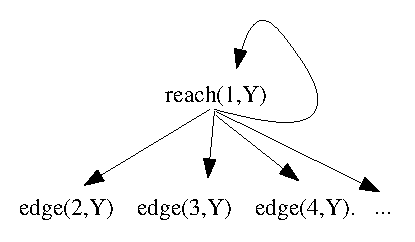
\includegraphics[width=\textwidth]{recursion}
%  \caption{Without \abstraction}
%  \label{fig:minipage1}
\end{minipage}
\quad
\begin{minipage}[b]{0.25\linewidth}
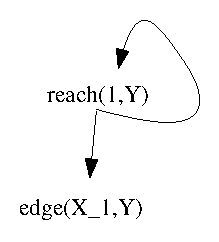
\includegraphics[width=0.5\textwidth]{abs-recursion}
%  \caption{With \abstraction}
%  \label{fig:minipage2}
\end{minipage}
\caption{A left-linear program and schematic IDGs: Left
  without IDG abstraction; Right: with
  IDG abstraction} \label{fig:abstraction}
\end{figure}
%------------------------------------------------------------
Abstracting the {\tt edge/2} predicate has subtle differences from
abstracting tabled subgoals.
%  The implementation of subgoal
%abstraction for tabled subgoals was described in~\cite{RigS13},
As mentioned, the {\tt edge/2} predicate of
Fig.~\ref{fig:abstraction} is not tabled.  Furthermore, the actual
{\tt edge/2} subgoal itself should not be abstracted to depth 0 since
losing the first argument instantiation would prevent the use of
indexing.  Rather, only the IDG's representation of the subgoal
should be abstracted.  Abstraction of dynamic code for
the IDG can be specified via the declaration:
\begin{center}
{\tt :-dynamic edge/2 as incremental, abstract(0)}.
\end{center}

In \version{} dynamic incremental code can be abstracted, but
incremental interned tries (Section~\ref{sec:incr-update-tries})
cannot be.  Also, currently only depth 0 abstraction is supported.

\subsection{Summary and Implementation Status}
%
%When using incremental tabling, an application will most commonly need
%only the default transparent approach, although in special
%circumstances eager updating may be desired.  

The main design choices of incremental tabling
are as usual what to table, and also what dynamic predicates or tries
should be made incremental.  In addition, performance optimizations
may be made through a mixture of subgoal abstraction and dynamic
predicate abstraction.  This optimization can be informed by use of
{\tt statistics/0} which includes summary information about the IDG,
or using the IDG inspection predicates of
Section~\ref{sec:incr-preds1} if more details are needed.

%Thus the user has four choices: tables may be
%updated as soon as the database is changed (e.g., via {\tt
%  incr\_assert/1}); at some point after a series of database changes
%(e.g. via {\tt incr\_assert\_inval/1} and {\tt
%  incr\_table\_update/0}); or lazily whenever a given table is called.
%In addition, if the changes are so massive that there is no point in
%incrementally updating the table, the tables can be abolished so that
%the tables will be reconstructed whenever they are re-queried.

In the current version of XSB, incremental tabling has not yet been
ported to the multi-threaded engine.  In addition, incremental tabling
only works for predicates that use both call and answer variance.
However, incremental tabling does work with for the full well-founded
semantics, for trie indexed dynamic code (in addition to regular
dynamic code) and with interned tries as described in
Section~\ref{sec:incr-update-tries}.  The space reclamation predicates
{\tt abolish\_all\_tables/0}, {\tt abolish\_table\_call/[1,2]} and
{\tt abolish\_table\_pred/[1,2]} can be safely used with incremental
tables.

\subsection{Predicates for Incremental Table Maintenance} \label{sec:incr-preds1}

\paragraph{A Note on Terminology}
%
Suppose {\tt p/1} and {\tt q/1} are incrementally tabled, and that
there is a clause
%
\begin{verbatim}
p(X):- q(X).
\end{verbatim}
%
In this case we say that {\tt p(X)} {\em depends\_on} {\tt q(X)} and
that {\tt q(X)} {\em affects} {\tt p(X)}.  A recursive predicate both
depends on and affects itself.


\paragraph{Declarations} The following directives support incremental
tabling based on changes in dynamic code: 

\index{tabling!opaque}
\index{tabling!declarations}
\begin{description}
\index{tabling!incremental}

\ourstandarditem{table +PredSpecs as incremental}{table/1}{Tabling}
%
is a executable predicate that indicates that each tabled predicate
specified in {\tt PredSpec} is to have its tables maintained
incrementally.  {\tt PredSpec} is a list of skeletons, i.e. open
terms, or {\tt Pred/Arity} specifications~\footnote{No explicit module
  references are allowed.}.  The tables must use call variance and
answer variance and must be compiled and loaded into the
single-threaded engine.  If a predicate is declared with tabling
attributes that are not supported with incremental tabling a
permission error is thrown.  This predicate implies that its arguments
are tabled predicates.  See page \pageref{table-declaration} for
further discussion of tabling options.

We also note that any tabled predicate that is called by a predicate
tabled as incremental must also be tabled as incremental or as opaque.
On the other hand, a dynamic predicate {\tt d/n} that is called by a
predicate tabled as incremental may or may not need to be declared as
incremental.  However if {\tt d/n} is not declared incremental, then
changes to it will not be propagated to incrementally maintained
tables.

\ourstandarditem{dynamic +PredSpecs as incremental}{dynamic/1}{Tabling}
%
is an executable predicate that indicates that each predicate in {\tt
  PredSpecs} is dynamic and used to define an incrementally tabled
predicate and will be updated using {\tt incr\_assert/1} and/or {\tt
  incr\_retractall/1} (or relatives.)  Note that dynamic incremental
predicates cannot themselves be tabled.  This predicate implies that
its arguments are dynamic predicates.  See page
\pageref{dynamic-declaration} for further discussion of dynamic
options.

\ourstandarditem{table +PredSpecs as opaque}{table/1}{Tabling} 
%
is an executable predicate that indicates that each predicate $P$ in
{\tt PredSpecs} is tabled and is used in the definition of some
incrementally tabled predicate but should not be maintained
incrementally.  In this case the system assumes that the programmer
will abolish tables for $P$ in such a way so that re-calling it will
always give semantically correct answers.  In other words, instead of
maintaining information to support incremental table maintenance, the
system re-calls the opaque predicate whenever its results are required
to recompute an answer.  One example of an appropriate use of opaque
is for tabled predicates in a DCG used to parse some string.  Rather
than incrementally maintain all dependencies on all input strings, the
user can declare these intermediate tables as opaque and abolish them
before any call to the DCG.  This predicate implies that its arguments
are tabled predicates.

\end{description}

\paragraph{Basic Incremental Maintenance Predicates}
The following predicates are used to manipulate incrementally
maintained tables:

\begin{description}
\ourrepeatmoditem{incr\_assert(+Clause)}{incr\_assert/1}{increval} 
\ourrepeatmoditem{incr\_assertz(+Clause)}{incr\_assertz/1}{increval}
\ourrepeatmoditem{incr\_asserta(+Clause)}{incr\_asserta/1}{increval}
\ourrepeatmoditem{incr\_retract(+Clause)}{incr\_retract/1}{increval}
\ourmoditem{incr\_retractall(+Term)}{incr\_retractall/1}{increval}
% 
are versions of {\tt assert/1} and other standard Prolog predicates.
They modify dynamic code just as their Prolog counterparts, but they
first invalidate all incrementally maintained tables that depend on
{\tt Clause}.

{\bf Error Cases} are the same as {\tt assert<a/z>/1}, {\tt retract/1}
and {\tt retractall/1} with the additional error conditions that
relate to the semantics of incremental tabling.  Note that if these
error conditions arise, the update will {\tt not} occur.

\begin{itemize}
\item The head of the clause {\tt Clause} or the {\tt Term} refers to
  a predicate that is not incremental and dynamic.  
\bi
\item  {\tt type error(dynamic\_incremental, Term)}
\ei
%
\item {\tt Clause} affects an incremental table that is incomplete
  (and so is in the course of being computed).
\bi
\item  {\tt permission\_error}
\ei 
\end{itemize}

%\ourrepeatmoditem{incr\_assert\_immed(+Clause)}{incr\_assert\_immed/1}{increval}
%\ourrepeatmoditem{incr\_assertz\_immed(+Clause)}{incr\_assertz\_immed/1}{increval}
%\ourrepeatmoditem{incr\_asserta\_immed(+Clause)}{incr\_asserta\_immed/1}{increval}\
%\ourrepeatmoditem{incr\_retractall\_immed(+Clause)}{incr\_retractall\_immed/1}{increval}
%\ourmoditem{incr\_retract\_immed(+Term)}{incr\_retract\_immed/1}{increval}
%%
%are versions of {\tt assert/1} and other standard Prolog predicates.
%They modify dynamic code just as their Prolog counterparts, mark any
%incrementally maintained tables that depend on the modification as
%invalid, then immediately update these tables.
%%  The tables may be updated by an
%explicit call to {\tt incr\_table\_immed/[0,1,2]}, or the table will
%be dynamically recomputed when a query is made to it.

%\ourmoditem{incr\_table\_update}{incr\_table\_update/0}{increval} may
%be called after base predicates have been changed (by {\tt
%  incr\_assert/1} and/or {\tt incr\_retract/1} or friends).  This
%predicate updates all the incrementally maintained tables whose
%contents may be affected by those changes to the base predicates.
%This update operation is separated from the operations that change the
%base predicates ({\tt incr\_assert\_inval/1} and {\tt
%  incr\_retractall\_inval/1}) so that a set of base predicate changes
%can be processed all at once, which may be much more efficient that
%updating the tables at every base update.  Beginning with Version
%3.3.7, it is not absolutely necessary to call this predicate, as
%tables will be incrementally updated upon demand.  However, using this
%predicate allows a choice of incurring the cost of update at a time
%other than querying an updated goal.
%Explicit update calls only need to be used in special circumstances
%(cf. Section~\ref{sec:incr-eager}).

%{\bf Error Cases}
%\bi
%\item A table $T$ that is to be incrementally updated is not yet
%  complete.  
%\bi
%\item 	{\tt permission\_error(update, incomplete\_table Goal)}
%\ei
%\item An abolish of some incremental table has made the global update
%  list potentially corrupted.
%\bi
%\item {\tt permission\_error}
%\ei 
%  \ei

%\ourmoditem{incr\_table\_update(-GoalList)}{incr\_table\_update/1}{increval}
%acts as {\tt incr\_table\_update/0} in its action to update the
%incrementally maintained tables after changes to base predicates.  It
%returns the list of goals whose tables were changed in the update
%process.
%
%\ourmoditem{incr\_table\_update(+SkelList,-GoalList)}{incr\_table\_update/2}{increval}
%acts as {\tt incr\_table\_update/1} in its action to update
%incrementally maintained tables after changes to base predicates.  The
%first argument is a list of predicate skeletons (open terms) for
%incrementally maintained tables.  The predicate returns in {\tt
%  GoalList} a list of goals whose skeletons appear in {\tt SkelList}
%and whose tables were changed in the update process.  In this way {\tt
%  SkelList} acts as a filter to restrict the goals that are returned
%to those of interest.  If {\tt SkelList} is a variable, all affected
%goals are returned in {\tt GoalList}.

\ourmoditem{incr\_invalidate\_call(+Goal)}{incr\_invalidate\_call/1}{increval}
Let $\cT$ be the least set of all incrementally maintained tables
whose goals that unify with {\tt Goal}, or whose tables are
(transitively) affected by a goal in $\cT$.  This predicate invalidates
all tables in $\cT$.  Any subsequent call to a goal $G$ associated
with $\cT$ will be automatically be incrementally updated if
necessary.  (As will any goals that $G$ depends on that are in need of
updating.)  In a similar manner, an invocation of {\tt
  incr\_table\_update/[0,1,2]} will cause tables in $\cT$ to be
updated.

Note that this predicate is needed for exceptional cases only.  Calls
to {\tt incr\_assert/1} and similar predicates mentioned above perform
invalidation automatically, as does {\tt abolish\_table\_call/[1,2]}.
However, {\tt incr\_invaldate\_calls/1} is useful if a tabled
predicate depends on some external data and not (only) on dynamic
incremental predicates.  For example, such a predicate might depend on
a relation stored in an external relational database (perhaps accessed
through the ODBC interface).
% then this predicate can be used to invalidate the
%table when the external relation changes.  
Of course, in such a case, the application programmer must know when
the external relation changes and invoke {\tt
  incr\_invalidate\_calls/1} as necessary.


{\bf Error Cases}
\bi
\item 	{\tt Goal} is tabled, but not incrementally tabled
\bi
\item 	{\tt permission\_error(invalidate,non-incremental predicate,Goal)}
\ei
\ei

\end{description}

\paragraph{Incremental Maintenance using Interned Tries}
The following predicates are used to modify incremental tries, and can
be freely intermixed with predicates for modifying incremental dynamic
code, as well as with predicates for invalidating or updating tables
(Section~\ref{sec:incr-preds1}).

\begin{description}
\ourmoditem{incr\_trie\_intern(+TrieIdOrAlias,+Term)}{incr\_trie\_intern/2}{intern}
%
is a version of {\tt trie\_intern/2} for tries declared as
incremental.  A call to this predicate interns {\tt Term} in {\tt
  TrieIdOrAlias} and then invalidates all incrementally maintained
tables that depend on this trie.

\ourmoditem{incr\_trie\_uninternall(+TrieIdOrAlias,+Term)}{incr\_trie\_uninternall/2}{intern}
%
is a version of {\tt trie\_unintern/2} for tries declared as
incremental.  A call to this predicate removes all terms unifying with
{\tt Term} in {\tt TrieIdOrAlias} and then invalidates all
incrementally maintained tables that depend on this trie.

%\ourmoditem{incr\_trie\_intern\_immed(+TrieIdOrAlias,+Term)}
%           {incr\_trie\_intern\_immed/2}{intern}
%%
%works for tries declared as incremental in a similar manner as {\tt
%  incr\_trie\_intern/2} except that it also immediatesly updates any
%affected tables.

%\ourmoditem{incr\_trie\_uninternall\_immed(+TrieIdOrAlias,+Term)}
%{incr\_trie\_uninternall\_immed/2}{intern}
%
%works for tries declared as incremental in a similar manner as {\tt
%  incr\_trie\_uninternall/2} except that it also immediately updates
%any affected tables.
\end{description}

\index{residual dependency graph}
\index{Incremental Dependency Graph (IDG)}
\paragraph{Inspecting the State of the Incremental Dependency Graph}
%
% These relations form a labelled directed graph for which the
%nodes are incrementally tabled subgoals present in XSB; a given
%subgoal in the graph may or may not have been completed.  
%Conceptually, there is an edge from $S_1$ to $S_2$ labelled depends
%(affects) if $S_1$ directly depends on (directly affects) $S_2$.  We
%call this graph the {\em incrementally tabled subgoal dependency
%  graph}, or just the incremental dependency graph.  
The predicates in this section allow a user to inspect properties of
IDG that can be useful in debugging, profiling or optimizing a
computation~\footnote{The predicates for traversing the incremental
  dependency graph are somewhat analogous to those for traversing the
  residual dependency graph (Section~\ref{sec:table-inspection}).}.
In addition they provide information about which subgoals in the IDG
are invalid -- i.e., which subgoals depend on a dynamic code that has
changed, but have not been updated.

As explained below, IDG nodes can be accessed via the predicate {\tt
  is\_incremental\_subgoal/1}, while IDG edges can be accessed via
{\tt incr\_directly\_depends/2}.  The predicates {\tt
  get\_incr\_scc/[1,2]} and {\tt get\_incr\_scc\_with\_deps/[3,4]} can
be used to efficiently materialize the dependency graph in Prolog,
including SCC information.  Similarly, the predicate {\tt
  subgoal\_property/2} can be used to determine which subgoals are
invalid.

\begin{description}

\ourmoditem{is\_incremental\_subgoal(?Subgoal)}{is\_incremental\_subgoal/1}{increval}
%
This predicate non-deterministically unifies {\tt Subgoal} with
incrementally tabled subgoals that are currently table entries.

\ourmoditem{incr\_directly\_depends(?Goal$_1$,?Goal$_2$)}{incr\_directly\_depends/2}{increval}
accesses the edges of the IDG: the incremental goals (Tables) that
directly depend on or directly affect one another.  At least one of
{\tt Goal$_1$} or {\tt Goal$_2$} must be bound.
\begin{itemize}
\item If {\tt Goal$_1$} is bound, then this predicate will return in
  {\tt Goal$_2$} through backtracking the goals for all incrementally
  maintained tables and dynamic leaf nodes on which {\tt Goal$_1$}
  directly depends.
\item If {\tt Goal$_2$} is bound, then it returns in {\tt Goal$_1$}
  through backtracking the goals for all incrementally maintained
  tables that {\tt Goal$_2$} directly affects -- in other words all
  goals that directly depend on {\tt Goal$_2$}.  \ei

{\bf Error Cases}
\bi
\item Neither {\tt Goal$_1$} nor {\tt Goal$_2$} is bound 
\bi
\item 	{\tt instatiation\_error}
\ei
\item {\tt Goal$_1$} and/or {\tt Goal$_2$} is bound, but is not
  incrementally tabled
\bi
\item 	{\tt table\_error}
\ei
\ei

\ourmoditem{incr\_trans\_depends(?Goal$_1$,?Goal$_2$)}{incr\_trans\_depends/2}{increval}
is similar to {\tt incr\_directly\_depends/2} except that it returns
goals according to the transitive closure of the ``directly depends''
Xrelation.  Error conditions are the same as {\tt
  incr\_directly\_depends/2}.

\ourmoditem{add\_incr\_dependency(Goal)}{add\_incr\_dependency/1}{increval}
%
Incremental tabling creates dependency graphs dynamically, so that
specific goal bindings can always be used.  This works well the great
majority of the time, but consider the following case:
\begin{verbatim}
:- dynamic p/1, q/2 as incremental.
:- table t1/2 as incremental.
t1(X,1):- p(X,Y),!.
t1(X,Y):- q(X,Y).

p(1,2).
\end{verbatim}
In the case of the goal {\tt ?- t1(1,Y)} the first clause will
succeed, cutting away the second clause so that the dependency of {\tt
  t1(1,Y)} on {\tt q(1,Y)} is never added, which may cause unexpected
behavior later in execution if new clauses are added or retracted for
{\tt q/1}.  Such a situation can be addressed using {\tt
  add\_inc\_dependency/2} by rewriting {\tt t1/2} as:
\begin{verbatim}
t1(X,Y):- p(X,Y),!,add_incr_dependency(q(X,Y)).
t1(X,Y):- q(X,Y).
\end{verbatim}
It must be stressed, however, that it should not be common to need {\tt
  add\_incr\_dependency/1} and it should be avoided in most (though not all) situations.

\ourrepeatmoditem{get\_incr\_sccs(?SCCList)}{get\_incr\_sccs/1}{increval}
\ourrepeatmoditem{get\_incr\_sccs\_with\_deps(?SCCList,?DepList)}{get\_incr\_sccs\_with\_deps/2}{increval}
\ourrepeatmoditem{get\_incr\_sccs(+SubgoalList,?SCCList)}{get\_incr\_sccs/2}{increval}
\ourmoditem{get\_incr\_sccs\_with\_deps(+SubgoalList,?SCCList,?DepList)}{get\_incr\_sccs\_with\_deps/3}{increval}
%

%{\bf {\em Warning: these predicates may be obsolescent, cf.
%    Section~\ref{sec:dep-graph} for newer predicates that are more
%    powerful.}}
%
%Most linear algorithms for SCC detection over a graph use destructive
%assignment on a stack to maintain information about the connectedness
%of a component; as a result such algorithms are
%difficult to write efficiently in Prolog.
%
%{\tt get\_incr\_sccs/1} unifies {\tt SCCList} with SCC information for
%the incremental dependency graph that is represented as a list whose
%elements are of the form
%\begin{center}
%{\tt ret(Subgoal,SCC)}.
%\end{center}
%{\tt SCC} is a numerical index for the SCCs of Subgoal. Two subgoals
%are in the same SCC iff they have the same index, however no other
%dependency information can be otherwise directly inferred from the
%index~\footnote{The actual number for each SCC index depends on how
%  the incremental dependency graph happens to be traversed; as a
%  result it is best to rely on the index only as a ``generated'' name
%  for each SCC.}.
%
%If dependency information is also desired, {\tt
%  get\_incr\_scc\_with\_dependencies/2} should be called.  In addition
%to the SCC information as above, {\tt DepList} is unified with a list
%of dependency terms of the form
%\begin{center}
%{\tt depends(SCC1,SCC2)}
%\end{center}
%for each pair {\tt SCC1} and {\tt SCC1} such that some subgoal with
%index {\tt SCC1} directly depends on some subgoal with index {\tt
%  SCC1}.  If it is necessary to know which subgoal(s) in {\tt SCC1}
%directly depends on which subgoal(s) in {\tt SCC2}, the information
%can be easily reconstructed using {\tt incr\_directly\_depends/2}
%above.  Similarly, {\tt incr\_directly\_depends/2} can be used to
%determine the actual edges within a given SCC.
%
%Ordinarily a user will want to see the entire dependency graph and in
%such a case the predicates described above should be used.  However,
%note that if the dependency graph is the result of several
%independent queries it may not be connected.  {\tt get\_incr\_scc/2}
%takes as input a list of incremental subgoals, {\tt SubgoalList}.  For
%each {\tt Subgoal} in {\tt SubgoalList}, this predicate finds the set
%of subgoals connected to {\tt Subgoal} by any mixture of depends and
%affects relations, unions these sets together, and finds the SCCs of
%all subgoals in the unioned set.
%
%SCC detection is implemented using Tarjan's algorithm~\cite{Tarj72} in
%C working directly on XSB's data structures.  The algorithm is
%\cO(|V| + |E|)$ where $|V|$ is the number of vertices and $|E|$ the
%number of edges in the dependency graph.  As a result, {\tt
%  get\_incr\_sccs/[1,2]} provides an efficient means to materialize the
%  high-level topography of the dependency graph~\footnote{Currently,
%    the materialization of dependency information between SCCs is
%    implemented in a naive manner, so that {\tt
%      get\_incr\_sccs\_with\_deps/[2,3]} is $\cO(|V|^2)$.}.%%%
%
%{\bf Error Cases}
%\bi
%\item {\tt SubgoalList} is a variable
%\bi
%\item 	{\tt instantiation\_error}
%\ei
%\item {\tt SubgoalList} is not a list
%\bi
%\item 	{\tt type\_error}%
%\ei
%\item {\tt SubgoalList} contains a predicate that is not tabled
%\bi
%\item 	{\tt permission\_error}
%\ei%
%\ei
%}
%\ourmoditem{incr\_invalid\_subgoals(-List)}{incr\_invalid\_subgoals/1}{increval}
%
%This predicate unifies {\tt List} with a sorted list of the
%incremental subgoals that are currently invalid.

%\ourmoditem{incr\_is\_invalid(+Subgoal)}{incr\_is\_invalid/1}{increval}
%
%Succeeds if {\tt Subgoal} is an incrementally tabled subgoal that is
%invalid, and fails otherwise.

\end{description}

 (included in tables)
\chapter[Standard and General Predicates]{Standard Predicates and Predicates of General Use} \label{standard}
%=============================================

This chapter mainly describes {\em standard} predicates, which are
always available to the Prolog interpreter, and do not need to be
imported or loaded explicitly as do other Prolog predicates.  By
default, it is a compiler error to redefine standard predicates.

\comment{This behavior can be overridden by allowing explicit
  redefinition of standard predicates (see Section~\ref{}); or
  alternatively the set of standard predicates can be easily
  reconfigured (Section~\ref{}).}

In the description below, certain standard predicates depend on HiLog
semantics; the description of such predicates have the token {\sf
HiLog} at the right of the page.  Similarly predicates that depend on
SLG evaluation are marked as {\sf Tabling}, and predicates whose
semantics is defined by the ISO standard (or whose implementation is
reasonably close to that definition) are marked as {\tt ISO}.
Occasionally, however, we include in this section predicates that are
not standard.  In such cases we denote their module in {\tt text} font
towards the middle of the page.

\comment{
\paragraph*{A Note on Types} \label{sec:types}

Numerous proposals have been made concerning typing systems for Prolog
for the purposes of program analysis, correctness checking, etc.
Analysis-based typing systems are typically lattice-based, following
from their need to compare types to understand whether one type
includes another, or from the need to determine the most specific type
that is more general than two types.  In addition the ISO standard
specifies various types of allowable input or output arguments for
various predicates.

\version{} of XSB has the following approach to program typing.
Typing in an XSB program is done through a {\em type lattice},
generated by {\em primitive type elements}.  How a primitive type is
defined is somewhat separate from how it is used by a type lattice.
For our purposes we assume that each 1-ary type element is defined by
a predicate of arity 1 that is written in a pure enough style so that
its success or failure does not depend on the state of XSB or of any
external state.  Whether these types are recursive or not has no
bearing on the type lattice.  For instance, {\tt integer} or {\tt
listOfAtoms} are primitive type elements.  Similarly, {\tt variable},
{\tt ground} are also type elements.  We say that a given term {\tt
Term} satisfies a primitive type element {\tt t} if {\tt t(Term)}
succeeds.  Given primitive type elements, complex type elements can be
formed using the boolean operations, {\tt and}, {\tt or} and {\tt
not}.  As an example, {\tt integer or not(listOfAtoms)} is a
non-primitive type element.  There is also a product operation ({\tt
,}) on type elements, so that {\tt variable, integer or
not(listOfAtoms)} is a product of the above two types.  
Satisfiability is extended to complex type elements in the obvious
manner, and an n-ary tuple of terms satisfies a n-ary product type if
each argument in the tuple satisfies the corresponding argument of the
product type.

The above description is not yet suitable for a type system as it
could not determine, for instance, that {\tt integer} is a subtype of
{\tt number}.  To determine this, an explicit {\em inclusion
statement} can be made indicating that one type is included in
another.  Thus given two elements in a type lattice with inclusion
statements, determining whether one element is more specific than
another can be done using techniques for propositional satisfiability
or stable model generation.

From an implementational level, types can be defined using the Cold
Dead Fish (CDF) package and inclusion can be detected using the CDF
theorem prover or XSB's Smodels interface.  However, for the
purposes in this section we use type elements to define inputs and
outputs of predicates, via {\tt usage statements}.  A usage statement
for an n-ary predicate {\tt p/n} consists of an n-ary product of
primitive types that should be satisfied on a call to {\tt p/n} along
with a n-ary product of primitive types that should hold on success of
{\tt p/n} given the types that hold at call.  If both the the product
types hold, the usage statement is satisfied.  Each successful call to
{\tt p/n} should satisfy one of the usage statements.

As defined, usage statements are very general: they can check not only
traditional Prolog types ({\tt atom}, {\tt integer}, etc), but also
non-Prolog types, such as the fact that the input to a given argument
should be a positive integer, and even instantiation patterns.  For
the various predicates defined in this section, we use the following
conventions for usages and error reporting.  {\bf domain}, {\bf type}
and {\bf instantiation} errors arise from the failure of an argument
of a predicate to satisfy the corresponding type element in the input
term of the usage statements.  All of these could be called type
errors given the system described above.  However to (partially)
conform to the ISO standard, we reserve the {\bf instantiation error}
to mean failure that occurs when an argument does not satisfy a type
in a boolean lattice generated by {\tt var} and {\tt ground}.  A {\bf
  type error} occurs when an argument does not satisfy a type in a
boolean lattice generated by other ISO types, such as {\tt integer},
{\tt atom}, etc.  A {\bf domain error} arises from other such errors.
We note that in certain cases, our designation of an error type may
differ from the ISO standard.
}

%--------------------------------------------------------------------------------------------------
\section{Input and Output}
\index{streams}

\subsection{I/O Streams in XSB}
XSB's I/O is based on ISO-style streams, although it also supports
older DEC-10 style file handling.  The use of streams provides a
unified interface to a number of different classes of sources and
sinks.  Currently these classes include textual and binary files,
console input and output, pipes, and atoms; in the future sockets and
urls may be handled under the stream interface.  When streams are
opened, certain actions may occur depending on the class of the source
or sink and on the wishes of the user.  For instance when a file {\tt
F} is opened for output mode, an existing file {\tt F} may be
truncated (in write mode) or not (in append mode).  In addition,
various operations may or may not be valid depending on the class of
stream.  For instance, repositioning is valid for an atom or file but
not a pipe or console.

XSB provides several default I/O streams, which make it easier for a
user to embed XSB in other applications.  These streams include the
default input and output streams.  They also include the standard
error stream, to which XSB writes all error messages.  By default the
standard error stream is the same as the standard output stream, but
it can be redirected either by UNIX shell-style I/O redirection or by
the predicates {\tt file\_reopen/4} and {\tt file\_clone/3}.
Similarly there is the standard warning stream (to which all system
warnings are written), the standard message stream, the standard
debugging stream (to which debugging information is written), and the
standard feedback stream (for interpreter prompts, yes/no answers,
etc).  All of these streams are aliased by default to standard output,
and can be redirected by the predicates {\tt file\_reopen/4} and {\tt
  file\_clone/3}.  Such redirection can be useful for logging, or
other purposes.

\index{aliases!streams}
\index{aliases!streams!user\_input}
\index{aliases!streams!user\_output}
\index{aliases!streams!user\_error}
\index{aliases!streams!user\_warning}
\index{aliases!streams!user\_message}

Streams may also be aliased: the default input and output streams are
denoted by {\tt user\_input} and {\tt user\_output} and they refer to
the standard input and standard output streams of the
process \footnote{For backwards compatibility, the default input
  stream can also be aliased by {\tt user} or {\tt userin}, and the
  default output stream by {\tt user} or {\tt userout}.}.  Similarly,
XSB's error, warning and message streams uses the aliases {\tt
  user\_error}, {\tt user\_warning} and {\tt user\_message}
respectively.

Streams are distinguished by their {\tt class} -- whether they are
file or atom, etc.; as well as by various properties.  These
properties include whether a stream is positionable or not and whether
a (file) stream is textual or binary.

\bi
\item {\tt Console}: The default streams mentioned above are
console streams, which are textual and not repositionable.
%
\item {\tt File}:  A file stream corresponds to an operating system
file and is repositionable.  On Windows, binary files and textual
files differ, while on UNIX they are the same.  
%
\item {\tt Atom}: XSB can read from an atom, just as it can from a file.
Atoms are considered to be textual and repositionable.  Writing to
atoms via streams is not currently available in XSB, although 
the predicate {\tt term\_to\_atom/[2,3]} contains much of the
functionality that such streams would provide.

\item {\tt Pipe}: XSB can also open pipes either directly, or as part
of its ability to spawn processes.  When made into streams, pipes are
textual and not repositionable.
\ei

%------------------------------------------------------------------------------------------------
\subsubsection{I/O Stream Implementation} \label{sec:IO-streams}

A user may notice that XSB's I/O streams are small integers, but they
should not be confused with the file descriptors used by the OS.  The
OS file descriptors are objects returned by the C {\tt open} function;
XSB I/O streams indices into the internal XSB table of open files and
associated information. The OS does not know about XSB I/O streams,
while XSB (obviously) does know about the OS file descriptors. An OS
file descriptor may be returned by certain predicates (e.g.  {\tt
  pipe\_open/2} or user-defined I/O).  In the former case, a file
descriptor can be promoted to XSB stream by {\tt open/\{3,4\}} and in
the latter by using the predicate {\tt fd2iostream/2}.

When it starts, XSB opens a number of standard I/O streams that it
uses to print results, errors, debugging info, etc. The descriptors
are described in the file {\tt prolog\_includes/standard.h}. This file
provides the following symbolic definitions:
%%
\index{streams!system}
\index{streams!STDDBG}
\index{streams!STDERR}
\index{streams!STDFDBK}
\index{streams!STDIN}
\index{streams!STDOUT}
\index{streams!STDWARN}
\index{streams!STDMSG}
\index{streams!system}
\begin{verbatim}
    #define STDIN            0
    #define STDOUT           1
    #define STDERR           2
    #define STDWARN          3    /* output stream for xsb warnings  */
    #define STDMSG           4    /* output for regular xsb messages */
    #define STDDBG           5    /* output for debugging info       */
    #define STDFDBK          6    /* output for XSB feedback
                                     (prompt/yes/no/Aborting/answers) */

    #define AF_INET     0     /* XSB-side socket request for Internet domain */
    #define AF_UNIX     1     /* XSB-side socket request for UNIX domain */
\end{verbatim}
%%
%------------------------------------------------------------------------------------------
\comment{
In addition, the file \verb|emu/file_modes_xsb.h| provides the definitions
for the file opening modes:
%%
\begin{verbatim}
    #define OREAD          0    /* open for read           */
    #define OWRITE         1    /* open for write          */
    #define OAPPEND        2    /* open for append         */
    #define OSTRINGR       3    /* open string for reading */
    #define OSTRINGW       4    /* open string for writing (not implemented) */
\end{verbatim}
%%
}
%------------------------------------------------------------------------------------------
These definitions can be used in user programs, if the following is
provided at the top of the source file:
%%
\begin{verbatim}
    compiler_options([xpp_on]).
    #include "standard.h"
\end{verbatim}
%%
If this header is used, the various streams can be used as any other output stream -- e.g. 
{\tt ?- write(STDWARN,'watch it!')}.
%
(Note: the XSB preprocessor is not invoked on clauses typed into an
interactive XSB session, so the above applies only to programs loaded
from a file using {\tt consult} and such.)

\subsection{Character Sets in XSB}\label{sec-charsets}
%
\index{Unicode!UTF-8}
\index{character sets}
\index{CP1252}
\index{LATIN-1}
Beginning in Version 3.5 of XSB, alternate character sets are supported.  
%
\begin{itemize}
\item {\em UTF-8} which on input automatically interprets the sequence
of bytes as UTF-8 byte sequences and decodes them to obtain the
unicode code points; and on output converts from the unicode code
points to UTF-8 byte sequences.
%
\item {\em LATIN-1} which performs no transformation on byte sequences 
(i.e. treats each byte directly as a unicode code point.)
%
\item {\em CP1252} which implements Windows code page 1252 encoding, the 
default for most Windows systems.
\end{itemize}

Other character sets, in particular UTF-16, may be supported in the
future.

In the current version of XSB, UTF-8 is the default character set when
XSB is configured on UNIX-style systems such as Linux and Mac OSX.
CP1252 is the default character set on Windows-style systems.  The
character set may be changed at any time via the Prolog flag {\tt
  character\_set}, whose value must be one of {\tt utf\_8}, {\tt
  cp1252}, or {\tt latin\_1}.  The character set that is in effect at
the time of opening a stream is the character set that will be used to
read (or write) the stream.  When XSB source code files are read by
the compiler (or by {\tt load\_dyn\_gen/2}), their encoding is assumed
to {\tt utf\_8} for all operating systems.  Note, however, that the
{\tt encoding/1} directive (\ref{other-directives}) can be placed in a
source file to change the encoding used by the compiler to read the
(remainder of the) file.


\subsection{Predicates for ISO Streams}

\begin{description}

\isoitem{open(+SourceSink,+Mode,-Stream)}{open/3}
%
{\tt open/1} creates a stream for the source or sink designated in
{\tt SourceSink}, and binds {\tt Stream} to a structure representing
that stream.  
%
\bi
\item If {\tt SourceSink} is an atom, or the term {\tt file(File)}
where {\tt File} is an atom, the stream is a file stream.  In this
case {\tt Mode} can be 
\bi
\item {\tt read} to create an input stream.  In Windows, whether the
file is textual or binary is determined by the file's properties.
%
\item {\tt write} to create an output stream.  Any previous file with
a similar path is removed and a (textual) file is created which becomes
a record of the output stream.  
%
\item {\tt write\_binary} to create an output stream.  Any previous file with
a similar path is removed and a file is created which becomes
a record of the output stream.  The file created is binary in Windows,
while in UNIX {\tt write\_binary} has the same effect as {\tt write}.
%
\item {\tt append} to create an output stream.  In this case the
output stream is appended to the contents of the file, if it exists,
and otherwise a new file is created for (textual) output
%
\item {\tt append\_binary} to create an output stream.  In this case the
output stream is appended to the contents of the file, if it exists,
and otherwise a new file is created for (binary) output
\ei
\item If {\tt SourceSink} is the term {\tt atom(Atom)} where {\tt
Atom} is an atom, the stream is an atom stream.  In this case {\tt
Mode} currently can only be {\tt read}.  This stream class, which
reads from interned atoms, is analogous to C's {\tt sscanf()}
function.
%
\item If {\tt SourceSink} is the term {\tt pipe(FileDescriptor)}
where {\tt FileDescriptor} is an integer, then a pipe stream is opened
in the mode for {\tt FileDescriptor}.
\ei

\compatibility This predicate extends the ISO definition of {\tt
open/3} to include strings and pipes as well as the file modes {\tt
write\_binary} and {\tt append\_binary}.

{\bf Error Cases}
\bi
\item 	{\tt SourceSink} or {\tt Mode} is not instantiated
\bi
\item 	{\tt instantiation\_error}
\ei
%
\item 	{\tt Mode} is not a valid I/O mode
\bi
\item 	{\tt domain\_error(io\_mode,Mode)}
\ei
%
\item {\tt SourceSink} is a file and cannot be opened, or opened in
  the desired mode, does not exist, etc.
\bi
\item 	{\tt permission\_error(open,file,SourceSink)}
\ei
\ei

\isoitem{open(+File,+Mode,-Stream,+Options)}{open/4}
%
{\tt open/4} behaves as does {\tt open/3}, but allows a list of
options to be given.  The current options are a subset of ISO options
and are:
\bi
\item {\tt alias(A)} allows the stream to be aliased to an atom {\tt
  A}.
%
\item {\tt type(T)} has no effect on file streams in UNIX, which are
  always textual, but in Windows if {\tt T} is {\tt binary} a binary
  file is opened.
\ei
%
{\bf Error Cases}  Error cases are the same as {\tt open/3} but with
the addition: 
\bi
\item {\tt Option\_list} contains an option {\tt O} that is not a
  (currently implemented) stream option.  
\bi
\item {\tt domain\_error(stream\_option,O)}
\ei
\item An element of {\tt OptionsList} is alias(A) and A is already
  associated with an existing
  %thread,
  queue, mutex or stream 
\bi
\item {\tt permission\_error(create,alias, A)}
\ei
\item An element of {\tt OptionsList} is alias(A) and A is not an atom
\bi
\item {\tt type\_error(atom,A)}
\ei
\ei
%
\compatibility 
%
The ISO option {\tt reposition(Boolean)} currently has no effect on
streams, because whether or not the stream is repositionable or not
depends on the stream class.  The ISO option {\tt eof\_action(Action)}
currently has no effect on file streams.  If these options are
encountered in {\tt Options}, a warning is issued to {\tt STDWARN}.

\isoitem{close(+Stream\_or\_alias,+OptionsList)}{close/2}
%
{\tt close/2} closes the stream or alias {\tt Stream\_or\_alias}.
{\tt OptionsList} allows the user to declare whether a permission
error will be raised in XSB upon a resource or system error from the
closing function (e.g. {\tt fclose()} or other system function).  If
{\tt OptionsList} is non-empty and contains only terms unifying with
{\tt force(true)} then such an error will be ignored (possibly leading
to unacknowledged loss of data).  Otherwise, a permission error is
thrown if {\tt fclose()} or other system function returns an error
condition.  If the stream class of {\tt Stream\_or\_alias} is an atom,
then the only action taken is to close the stream itself -- the
interned atom itself is not affected.

{\bf Error Cases}
\bi
\item 	{\tt Stream\_or\_alias} is a variable
\bi
\item {\tt instantiation\_error}
\ei
\item {\tt Stream\_or\_alias} is neither a variable, nor a stream term
  nor an alias.  
\bi
\item 	{\tt domain\_error(stream\_or\_alias,Stream\_or\_alias)}
\ei
\item 	{\tt Stream\_or\_alias} is not associated with an open stream
\bi
\item 	{\tt existence\_error(stream,Stream\_or\_alias)}
\ei
\item {\tt OptionList} contains an option {\tt O} that is not a closing
option.
\bi
\item {\tt domain\_error(close\_option,O)}
\ei
\item {\tt OptionList} contains conflicting options
\bi
\item {\tt domain\_error(close\_option,OptionList)}
\ei
\item 	Closing the stream produces an error (and {\tt OptionsList} is
	a non-empty list containing terms of the form {\tt force(true)}).
\bi
\item 	{\tt permission\_error(close,file,Stream\_or\_alias)}
\ei
\ei

\isoitem{close(+Stream\_or\_alias)}{close/1}
%
{\tt close/1} closes the stream or alias {\tt Stream\_or\_alias}.\\
Behaves as {\tt close(Stream\_or\_alias,[force(false)])}.

\isoitem{set\_input(+Stream\_or\_alias)}{set\_input/1}
    Makes file {\tt Stream\_or\_alias} the current input stream. 

{\bf Error Cases}
\bi
\item 	{\tt Stream\_or\_alias} is a variable
\bi
\item {\tt instantiation\_error}
\ei
\item {\tt Stream\_or\_alias} is neither a variable, nor a a stream
  term nor an alias.  
\bi
\item 	{\tt domain\_error(stream\_or\_alias,Stream\_or\_alias)}
\ei
\item 	{\tt Stream\_or\_alias} is not an open input stream
\bi
\item 	{\tt existence\_error(stream,Stream\_or\_alias)}
\ei
\ei

\isoitem{set\_output(+Stream\_or\_alias)}{set\_output/1}
    Makes file {\tt Stream\_or\_alias} the current output stream. 

{\bf Error Cases}
\bi
\item 	{\tt Stream\_or\_alias} is a variable
\bi
\item {\tt instantiation\_error}
\ei
\item {\tt Stream\_or\_alias} is neither a variable, nor a a stream
  term nor an alias.  
\bi
\item 	{\tt domain\_error(stream\_or\_alias,Stream\_or\_alias)}
\ei
\item 	{\tt Stream\_or\_alias} is not associated with an open output stream
\bi
\item 	{\tt existence\_error(stream,Stream\_or\_alias)}
\ei
\ei

\isoitem{stream\_property(?Stream,?Property)}{stream\_property/2}
%
This predicate backtracks through the various stream properties that
unify with {\tt Property} for the stream {\tt Stream}.  Currently,
the following properties are defined.

\bi
\item {\tt stream\_class(C)} gives the stream class for a file:
i.e. {\tt file}, {\tt atom}, {\tt console} or {\tt pipe}.

\item {\tt file\_name(F)} is a property of {\tt Stream}, if
{\tt Stream} is a file stream and {\tt F} is the file name
associate with {\tt Stream}.  The full operating system
path is used.
%
\item {\tt type(T)} is a property of {\tt Stream}, if
{\tt Stream} is a file stream and {\tt T} is the file type
of {\tt Stream}: {\tt text} or {\tt binary}.
%
\item {\tt mode(M)} is a property of {\tt Stream}, if {\tt
M} represents the I/O mode with which {\tt Stream} was
opened: i.e. {\tt read}, {\tt write}, {\tt append}, {\tt
write\_binary}, etc., as appropriate for the class of {\tt
Stream}.
%
\item {\tt alias(A)}  is a property of {\tt Stream}, if
{\tt Stream} was opened with alias {\tt A}.
%
\item {\tt input}  is a property of {\tt Stream}, if {\tt
Stream} was opened in the I/O mode: {\tt read}.
% 
\item {\tt output}  is a property of {\tt Stream}, if {\tt
Stream} was opened in the I/O mode: {\tt write}, {\tt
append}, {\tt write\_binary}, or {\tt append\_binary}.
%
\item {\tt reposition(Bool)} is true, if {\tt Stream} is
repositionable, and false otherwise. 
%
\item {\tt end\_of\_stream(E)} returns {\tt at} if the end of stream
condition for {\tt Stream} is true, and {\tt not} otherwise.
%
\item {\tt position(Pos)} returns the current position of the stream
as determined by {\tt fseek{}} or the byte-offset of the current
stream within an atom.  In either case, if an end-of-stream condition
occurs, the token {\tt end\_of\_file} is returned.
%

%
\item {\tt eof\_action(Action)} is {\tt reposition} if the stream class
is {\tt console}, {\tt eof\_code} if the stream class is {\tt file},
and {\tt error} is the stream class is {\tt pipe} or {\tt atom}.
\end{itemize}

\isoitem{flush\_output(+Stream\_or\_alias)}{flush\_output/1}
%
Any buffered data in {\tt Stream\_or\_alias}  gets flushed.  If
{\tt Stream} is not buffered (i.e. if it is of class {\tt
atom}), no action is taken.

{\bf Error Cases}
\bi
\item 	{\tt Stream\_or\_alias} is a variable
\bi
\item {\tt instantiation\_error}
\ei
\item {\tt Stream\_or\_alias} is neither a variable, nor a a stream
  term nor an alias.  
\bi
\item 	{\tt domain\_error(Stream\_or\_alias,Stream)}
\ei
\item 	{\tt Stream} is not associated with an open output stream 
\bi
\item 	{\tt existence\_error(Stream\_or\_alias,Stream)}
\ei
\item 	Flushing (i.e. {\tt fflush()}) returns an error.
\bi
\item 	{\tt permission\_error(flush,stream,Stream)}
\ei
\ei

\isoitem{flush\_output}{flush\_output/0}
%
Any buffered data in the current output stream gets flushed.

\isoitem{set\_stream\_position(+Stream\_or\_alias,+Position)}{set\_stream\_position/2}
%
If the stream associated with {\tt Stream\_or\_alias} is
repositionable (i.e. is a file or atom), sets the stream position
indicator for the next input or output operation. Position is a
positive integer, taken to be the number of bytes the stream is to be
placed from the origin.

{\bf Error Cases}
\bi
\item 	{\tt Stream\_or\_alias} is a variable
\bi
\item {\tt instantiation\_error}
\ei
\item {\tt Stream\_or\_alias} is neither a variable, nor a a stream
  term nor an alias.  
\bi
\item 	{\tt domain\_error(stream\_or\_alias,Stream\_or\_alias)}
\ei
\item 	{\tt Position} is not instantiated to a positive integer.
\bi
\item 	{\tt domain\_error(stream\_position,Position)}
\ei
\item 	{\tt Stream\_or\_alias} is not associated with an open stream
\bi
\item 	{\tt existence\_error(stream,Stream\_or\_alias)}
\ei
\item 	{\tt Stream\_or\_alias} is not repositionable, or
	repositioning returns an error. 
\bi
\item 	{\tt permission\_error(resposition,stream,Stream\_or\_alias)}
\ei
\ei



\isoitem{at\_end\_of\_stream(+Stream\_or\_alias)}{at\_end\_of\_stream/1}
%
Succeeds if {\tt Stream\_or\_alias} has position at or past the end of
stream.

{\bf Error Cases}
\bi
\item 	{\tt Stream\_or\_alias} is a variable
\bi
\item {\tt instantiation\_error}
\ei
\item {\tt Stream\_or\_alias} is neither a variable, nor a a stream
  term nor an alias.  
\bi
\item 	{\tt domain\_error(stream,Stream\_or\_alias)}
\ei
\item 	{\tt Stream\_or\_alias} is not an open stream
\bi
\item 	{\tt existence\_error(stream,Stream\_or\_alias)}
\ei
\ei
%

\isoitem{at\_end\_of\_stream}{at\_end\_of\_stream/0}
%
Acts as {\tt at\_end\_of\_stream/1} but using the current input
stream.

\end{description}

\subsubsection{Other Predicates using ISO Streams}

\begin{description}

\standarditem{file\_reopen(+FileName,+Mode,+Stream,-RetCode)}{file\_reopen/3}
%
    Takes an existing I/O stream, closes it, then opens it and
    attaches it to a file. This can be used to redirect I/O from any of the
    standard streams to a file. For instance, 
%%
\begin{verbatim}
    | ?- file_reopen('/dev/null', w, 3, Error).
\end{verbatim}
%%
    redirects all warnings to the Unix black hole. 

    On success, {\tt RetCode} is 0; on error, the return code is negative.

%-----------------------------------------------------------------------------

\standarditem{file\_clone(+SrcStream,?DestStream,-RetCode)}{file\_clone/3}
%
This is yet another way to redirect I/O. It is a Prolog interface to
the C {\tt dup} and {\tt dup2} system calls. If {\tt DestStream} is a
variable, then this call creates a new XSB I/O stream that is a clone
of {\tt SrcStream}. This means that I/O sent to either stream goes
to the same place. If {\tt DestStream} is not a variable, then it must
be a number corresponding to a valid I/O stream. In this case, XSB
closes {\tt DestStream} and makes it into a clone of {\tt
SrcStream}. 

For instance, suppose that 10 is a I/O Stream that is currently open
for writing to file {\tt foo.bar}.  Then 
%%
\begin{verbatim} 
| ?- file_clone(10,3,_).  
\end{verbatim} 
%% 
causes all messages sent to XSB standard warnings stream to go to file
{\tt foo.bar}. While this could be also done with {\tt file\_reopen},
there are things that only {\tt file\_clone} can do: 
%%
\begin{verbatim} 
| ?- file_clone(1,10,_). 
\end{verbatim} 
%% 
This means that I/O stream 10 now becomes clone of standard
output. So, all subsequent I/O will now go to standard output instead
of {\tt foo.bar}.

On success, {\tt RetCode} is 0; on error, the return code is negative.

%-----------------------------------------------------------------------------

\ourmoditem{file\_truncate(+Stream, +Length, -Return)}{file\_truncate/3}{file\_io}
    The regular file  referenced by the Stream{\tt Stream}
    is chopped to have the size of {\tt Length} bytes. Upon successful
    completion {\tt Return} is set to zero.

\portability Under Windows (including Cygwin) {\tt file\_truncate/2}
is implemented using {\tt \_chsize()}, while on Unix {\tt ftruncate()}
is used.  There are minor semantic differences between these two
system calls, which are reflected by the behavior of {\tt
file\_truncate/2} on different platforms.

{\bf Error Cases}
\bi
\item 	{\tt Stream\_or\_alias} is a variable
\bi
\item {\tt instantiation\_error}
\ei
\item {\tt Stream\_or\_alias} is neither a variable, nor a a stream
  term nor an alias.  
\bi
\item 	{\tt domain\_error(stream\_or\_alias,Stream\_or\_alias)}
\ei
\item 	{\tt Stream\_or\_alias} is not associated with an open stream
\bi
\item 	{\tt existence\_error(stream,Stream\_or\_alias)}
\ei
\item {\tt Length} is a variable
\bi
\item {\tt instantiation\_error}
\ei
\item {\tt Length} is neither a variable nor an integer
\bi
\item 	{\tt type\_error(integer,Length)}
\ei
\ei
\comment{Not checking for uninstantiated Return or for negative Length}

\standarditem{tmpfile\_open(-Stream)}{tmpfile\_open/1}
    Opens a temporary file with a unique filename. The file is deleted
    when it is closed or when the program terminates.

\ourmoditem{flush\_all\_output\_streams}{flush\_all\_output\_streams/0}{error\_handler}
\index{streams!system} 
%
Flushes output streams, both user and system {\tt STDOUT}, {\tt
  STDERR}, etc.  This convenience predicate is written as
%
\begin{verbatim}
flush_all_open_streams:- 
        stream_property(S,mode(X)),(X = append ; X = write),flush_output(S),fail.
flush_all_open_streams.
\end{verbatim}

\end{description}

\subsection{DEC-IO Style File Handling}

\begin{description}
\standarditem{see(+File\_or\_stream)}{see/1}
%
Makes {\tt File\_or\_stream} the current input stream. 
%
\begin{itemize}
\item If there is an open input stream associated with the file that
  has {\tt File\_or\_stream} as its file name, and that stream was
  opened previously, then it is made the current input stream.
%
\item Otherwise, the specified file is opened for input and made the
  current input stream. If the file does not exist, {\tt see/1} throws
  a permission error.
\end{itemize}
%
Note that {\tt see/1} is incompatible with ISO aliases -- calling {\tt
  see(Alias)} with an ISO alias will try to open a file named {\tt
  Alias} rather than using the alias.  Also note that different file
names (that is, names which do not unify) represent different input
streams (even if these different file names correspond to the same
file).

{\bf Error Cases}
\bi
\item  {\tt File\_or\_stream} is  a variable
\bi
\item {\tt instantiation\_error}
\ei
\item {\tt File\_or\_stream} is neither a variable nor an atomic file identifier nor
  a stream identifier.
\bi
\item {\tt domain\_error(stream\_or\_path,F)}
\ei
\item File {\tt File\_or\_stream} is directory or file is not readable. 
\bi
\item {\tt permission\_error(open,file,F)}
\ei
\item File {\tt File\_or\_stream} does not exist. 
\bi
\item {\tt existence\_error(stream\_or\_path,F)}
\ei
\ei

\standarditem{seeing(?F)}{seeing/1}
    {\tt F} is unified with the name of the current input stream.
    This is exactly the same with predicate {\tt current\_input/1}
    described in Section~\ref{State}, and it is only provided for
    upwards compatibility reasons.

\standarditem{seen}{seen/0}
    Closes the current input stream. 
    Current input reverts to {\tt ``userin''} (the standard input stream).

\standarditem{tell(+F)}{tell/1}
    Makes file {\tt F} the current output stream. 
    \begin{itemize}
    \item If there is an open output stream associated with {\em F}  
          and that was opened previously 
          by {\tt tell/1}, then that stream is made the current output 
	  stream. 
    \item Otherwise, the specified file is opened for output and made the
          current output stream. If the file does not exist, it is created.
    \end{itemize}

    Also note that different file names (that is, names which do not unify) 
    represent different output streams (even if these different file names 
    correspond to the same file).

    The implementation of the ISO predicate {\tt set\_output/1}, is
    essentially that of {\tt tell/1}.

{\bf Error Cases}
\bi
\item  {\tt File\_or\_stream} is  a variable
\bi
\item {\tt instantiation\_error}
\ei
\item {\tt File\_or\_stream} is neither a variable nor an atomic file identifier nor
  a stream identifier.
\bi
\item {\tt domain\_error(stream\_or\_path,F)}
\ei
\item File {\tt File\_or\_stream} is directory or file is not readable. 
\bi
\item {\tt permission\_error(open,file,F)}
\ei
\item File {\tt File\_or\_stream} does not exist. 
\bi
\item {\tt existence\_error(stream\_or\_path,F)}
\ei
\ei

\standarditem{telling(?F)}{telling/1}
    {\tt F} is unified with the name of the current output stream.
    This predicate is exactly the same with predicate {\tt current\_output/1}
    described in Section~\ref{State}, and it is only provided for
    upwards compatibility reasons.

\standarditem{told}{told/0}
    Closes the current output stream. 
    Current output stream reverts to ``userout'' (the standard output stream).

\standarditem{file\_exists(+F)}{file\_exists/1}
    Succeeds if file {\tt F} exists. {\tt F} must be instantiated to
    an atom at the time of the call, or an error message is displayed on
    the standard error stream and the predicate aborts.

{\bf Error Cases}
    \begin {description}
    \item[{\tt instantiation\_error}]
	{\tt F} is uninstantiated.
    \end{description}

\standarditem{url\_encode(+Filename,-EncodedFilename)}{url\_encode/2}
   This predicate is useful when one needs to create a file whose name
   contains forbidden characters, such as \texttt{>}, \texttt{<}, and the
   like. It takes a string and encodes any forbidden character
   using an appropriate \%-sequence of characters that is acceptable as a
   file name in any OS: Unix, Windows, or Mac.
   For instance, 
   %% 
\begin{verbatim}
   | ?- url_encode('http://foo''>$',X).

   X = http%3a%2f%2ffoo%27%3e%24
\end{verbatim}
   %% 

\standarditem{url\_decode(+Filename,-EncodedFilename)}{url\_decode/2}
   This predicate performs the inverse operation with respect to 
   \texttt{url\_encode/2}. For instance, 
   %% 
\begin{verbatim}
   | ?- url_decode('http%3a%2f%2ffoo%27%3e%24',X).

   X = http://foo'>$
\end{verbatim}
   %% 

\end{description}

\index{Unicode!UTF-8}
\subsection{Character I/O}
Beginning with \version{}, XSB supports Unicode in the form of UTF-8
characters.  Due to this change, we recommend using ISO-compliant
character I/O predicates, rather than older predicates such as {\tt
  get/1}, {\tt get0/1}, {\tt put/1} and so on.  As the use of these
older predicates may sometimes give unexpected answers when used with
non-ASCII characters, they are deprecated, although they are still
available for backward compatibility.

\begin{description}
%-----------------------------
% Gets

\isoitem{get\_char(+Stream\_or\_alias,?Char)}{get\_char/2} Unifies
        {\tt Char} with the next UTF-8 character from {\tt
          Stream\_or\_alias}, advancing the position of the stream.
        {\tt Char} is unified with the atom {\tt end\_of\_file} if an
        end of file condition is detected.

{\bf Error Cases}
\bi
\item 	{\tt Stream\_or\_alias} is a variable
\bi
\item {\tt instantiation\_error}
\ei
\item 	{\tt Stream\_or\_alias} is neither a variable nor a stream term nor an alias.
\bi
\item 	{\tt domain\_error(stream\_or\_alias,Stream\_or\_alias)}
\ei
\item 	{\tt Stream\_or\_alias} is not associated with an open input stream
\bi
\item 	{\tt existence\_error(stream,Stream\_or\_alias)}
\ei
\item 	{\tt Char} is not a variable or character.
\bi
\item 	{\tt domain\_error(character\_or\_variable,Char)}
\ei
\ei

\isoitem{get\_char(?Char)}{get\_char/1}
%
Behaves as {\tt get\_char/2}, but reads from the current input stream.

{\bf Error Cases}
\bi
\item 	{\tt Char} is not a variable or character.
\bi
\item 	{\tt domain\_error(character\_or\_variable,Char)}
\ei
\ei

\isoitem{get\_code(+Stream\_or\_alias,?Code)}{get\_code/2}
%
   {\tt Code} unifies with the UTF-8 code of the next character from
   {\tt Stream\_or\_alias}.  The position of the stream is advanced.
   {\tt Char} is unified with -1 if an end of file condition is
   detected.

{\bf Error Cases}
\bi
\item 	{\tt Stream\_or\_alias} is a variable
\bi
\item {\tt instantiation\_error}
\ei
\item 	{\tt Stream\_or\_alias} is neither a variable nor a stream term nor an alias.
\bi
\item 	{\tt domain\_error(stream\_or\_alias,Stream\_or\_alias)}
\ei
\item 	{\tt Stream\_or\_alias} is not associated with an open input stream
\bi
\item 	{\tt existence\_error(stream,Stream\_or\_alias)}
\ei
\item 	{\tt Code} is not a variable or character code
\bi
\item 	{\tt domain\_error(character\_code\_or\_variable,Code)}
\ei
\ei

\isoitem{get\_code(?Code)}{get\_code/1}
%
Behaves as {\tt get\_code/2}, but reads from the current input
stream~\footnote{The obsolescent predicate {\tt get0/1} is defined as
  {\tt get\_code/1}.}.

{\bf Error Cases}
\bi
\item 	{\tt Code} is not a variable or character code
\bi
\item 	{\tt domain\_error(character\_code\_or\_variable,Code)}
\ei
\ei

\isoitem{get\_byte(+Stream\_or\_alias,?Byte)}{get\_byte/2}
%
   {\tt Byte} unifies with the value of the the next byte from {\tt
     Stream\_or\_alias}.  The position of the stream is advanced.
   {\tt Char} is unified with -1 if an end of file condition is
   detected.  If reading from ASCII text, {\tt get\_byte/2} will have
   the same behavior as {\tt get\_code/2}, but in general {\tt
     get\_code/2} may return multi-byte characters

{\bf Error Cases}
\bi
\item 	{\tt Stream\_or\_alias} is a variable
\bi
\item {\tt instantiation\_error}
\ei
\item 	{\tt Stream\_or\_alias} is neither a variable nor a stream term nor an alias.
\bi
\item 	{\tt domain\_error(stream\_or\_alias,Stream\_or\_alias)}
\ei
\item 	{\tt Stream\_or\_alias} is not associated with an open input stream
\bi
\item 	{\tt existence\_error(stream,Stream\_or\_alias)}
\ei
\item 	{\tt Code} is not a variable or character code
\bi
\item 	{\tt domain\_error(character\_code\_or\_variable,Code)}
\ei
\ei

\isoitem{get\_byte/1}{get\_byte/1} Behaves as {\tt get\_byte/2}, but
reads from the current input stream~\footnote{The obsolescent
  predicate {\tt get0/1} is defined using {\tt get\_byte/1}, but
  returns the next byte that does not match an ASCII whitespace
  character.}.v

{\bf Error Cases}
\bi
\item 	{\tt Code} is not a variable or {\tt Code} is not a proper value for a byte
\bi
\item 	{\tt domain\_error(byte\_code\_or\_variable,Code)}
\ei
\ei

%\standarditem{get0(?N)}{get0/1}
%
%{\tt N} is the ASCII code of the next character read from the current
%input stream (regarded as a text stream). If the current input stream
%reaches its end of file, a {\tt -1} is returned.  This predicate does
%not check for errors, so that it is faster (and potentially less safe)
%than, e.g. {\tt get\_code/1}.

%\standarditem{get(?N)}{get/1}
%    {\tt N} is the ASCII code of the next non-blank printable
%    character from the current input stream (regarded as a text
%    stream).  If the current input stream reaches its end of file, a
%    {\tt -1} is returned.

%------------------------------------
% Peeks

\isoitem{peek\_char(+Stream\_or\_alias,?Char)}{peek\_char/2}
%
Unifies {\tt Char} with the next UTF-8 character from {\tt
  Stream\_or\_alias}.  The position in {\tt Stream\_or\_alias} is
unchanged.  {\tt Char} is unified with the atom {\tt end\_of\_file} if
an end of file condition is detected.

{\bf Error Cases}
\bi
\item 	{\tt Stream\_or\_alias} is a variable
\bi
\item {\tt instantiation\_error}
\ei
\item 	{\tt Stream\_or\_alias} is neither a variable nor a stream term nor an alias.
\bi
\item 	{\tt domain\_error(stream\_or\_alias,Stream\_or\_alias)}
\ei
\item 	{\tt Stream\_or\_alias} is not associated with an open input stream
\bi
\item 	{\tt existence\_error(stream,Stream\_or\_alias)}
\ei
\item 	{\tt Char} is not a variable or character.
\bi
\item 	{\tt domain\_error(character\_or\_variable,Char)}
\ei
\ei

\isoitem{peek\_char(?Char)}{peek\_char/1}
%
Behaves as {\tt peek\_char/2}, but the current input stream is used.

{\bf Error Cases}
\bi
\item 	{\tt Char} is not a variable or character.
\bi
\item 	{\tt domain\_error(character\_or\_variable,Char)}
\ei
\ei

\isoitem{peek\_code(+Stream\_or\_alias,?Code)}{peek\_code/2}
%
Unifies {\tt Code} with the next UTF-8 code from {\tt Stream\_or\_alias}.
The position in {\tt Stream\_or\_alias} is unchanged.  {\tt Code} is
unified with -1 if an end of file condition is detected.

{\bf Error Cases}
\bi
\item 	{\tt Stream\_or\_alias} is a variable
\bi
\item {\tt instantiation\_error}
\ei
\item 	{\tt Stream\_or\_alias} is neither a variable nor a stream term nor an alias.
\bi
\item 	{\tt domain\_error(stream\_or\_alias,Stream\_or\_alias)}
\ei
\item 	{\tt Stream\_or\_alias} is not associated with an open input stream
\bi
\item 	{\tt existence\_error(stream,Stream\_or\_alias)}
\ei
\item 	{\tt Code} is not a variable or character.
\bi
\item 	{\tt domain\_error(character\_code\_or\_variable,Code)}
\ei
\ei

\isoitem{peek\_code(?Code)}{peek\_code/1}
%
Behaves as {\tt peek\_code/2}, but the current input stream is used.

{\bf Error Cases}
\bi
\item 	{\tt Char} is not a variable or character.
\bi
\item 	{\tt domain\_error(character\_code\_or\_variable,Code)}
\ei
\ei

\isoitem{peek\_byte(?Byte)}{peek\_byte/1} 
%
Unifies {\tt Byte} with the next byte from {\tt Stream\_or\_alias}.
The position in {\tt Stream\_or\_alias} is unchanged.  {\tt Code} is
unified with -1 if an end of file condition is detected.

{\bf Error Cases}
\bi
\item 	{\tt Stream\_or\_alias} is a variable
\bi
\item {\tt instantiation\_error}
\ei
\item 	{\tt Stream\_or\_alias} is neither a variable nor a stream term nor an alias.
\bi
\item 	{\tt domain\_error(stream\_or\_alias,Stream\_or\_alias)}
\ei
\item 	{\tt Stream\_or\_alias} is not associated with an open input stream
\bi
\item 	{\tt existence\_error(stream,Stream\_or\_alias)}
\ei
\item 	{\tt Code} is not a variable or character.
\bi
\item 	{\tt domain\_error(byte\_code\_or\_variable,Code)}
\ei
\ei


\isoitem{peek\_byte(?Byte)}{peek\_byte/1}
Behaves as {\tt peek\_byte/2}, but the current input stream is used.

{\bf Error Cases}
\bi
\item 	{\tt Char} is not a variable or character.
\bi
\item 	{\tt domain\_error(byte\_code\_or\_variable,Code)}
\ei
\ei
%----------------------------------------------
% Puts
%----------------------------------------------

\isoitem{put\_char(+Stream\_or\_alias,+Char)}{put\_char/2}
%
Writes a UTF-8 character {\tt Char} to {\tt Stream\_or\_alias}.

{\bf Error Cases}
\bi
\item 	{\tt Stream\_or\_alias} is a variable
\bi
\item {\tt instantiation\_error}
\ei
\item 	{\tt Stream\_or\_alias} is neither a variable nor a stream term nor an alias.
\bi
\item 	{\tt domain\_error(stream\_or\_alias,Stream\_or\_alias)}
\ei
\item 	{\tt Stream\_or\_alias} is not associated with an open input stream
\bi
\item 	{\tt existence\_error(stream,Stream\_or\_alias)}
\ei
\item 	{\tt Char} is a not a character
\bi
\item 	{\tt type\_error(character,Char)}
\ei
\ei

\isoitem{put\_char(+Char)}{put\_char/1}
%
Puts a UTF-8 character {\tt Char} to the current output stream.

{\bf Error Cases}
\bi
\item 	{\tt Code} is a not a character.
\bi
\item 	{\tt type\_error(character,Char)}
\ei
\ei

\isoitem{put\_code(+Stream,+Code)}{put\_code/2}
%
Puts the character for the UTF-8 code {\tt Code} to {\tt
  Stream\_or\_alias}.

{\bf Error Cases}
\bi
\item 	{\tt Stream\_or\_alias} is a variable
\bi
\item {\tt instantiation\_error}
\ei
\item 	{\tt Stream\_or\_alias} is neither a variable nor a stream term nor an alias.
\bi
\item 	{\tt domain\_error(stream\_or\_alias,Stream\_or\_alias)}
\ei
\item 	{\tt Stream\_or\_alias} is not associated with an open input stream
\bi
\item 	{\tt existence\_error(stream,Stream\_or\_alias)}
\ei
\item 	{\tt Code} is a not a character code
\bi
\item 	{\tt type\_error(character\_code,Code)}
\ei
\ei


\isoitem{put\_code(+Code)}{put\_code/1}
%
Puts the character for the UTF-8 code {\tt Code} to the current output
stream~\footnote{The obsolescent predicate {\tt put/1} is defined as
  {\tt put\_code/1}.}.

{\bf Error Cases} \bi
\item 	{\tt Code} is a not a character code.
\bi
\item 	{\tt type\_error(character\_code,Code)}
\ei
\ei

%\standarditem{put(+Code)}{put/1}
%    Puts the ASCII character code {\tt N} to the current output stream.
%
%{\bf Error Cases}
%\bi
%\item 	{\tt Code} is a not a character code.
%\bi
%\item 	{\tt type\_error(character\_code,Code)}
%\ei
%\ei

\isoitem{nl}{nl/0}
A new line character is sent to the current output stream.

\isoitem{nl(+Stream\_or\_alias)}{nl/1}
A new line character is sent to the designated output stream.

{\bf Error Cases}
\bi
\item 	{\tt Stream\_or\_alias} is a variable
\bi
\item {\tt instantiation\_error}
\ei
\item 	{\tt Stream\_or\_alias} is neither a variable nor a stream term nor an alias.
\bi
\item 	{\tt domain\_error(stream\_or\_alias,Stream\_or\_alias)}
\ei
\item 	{\tt Stream\_or\_alias} is not associated with an open stream
\bi
\item 	{\tt existence\_error(stream,Stream\_or\_alias)}
\ei
\ei

\repeatstandarditem{tab(+Stream,+N)}{tab/2}
\standarditem{tab(+N)}{tab/1}
    Puts {\tt N} spaces to the designated output stream / current output stream. 

{\bf Error Cases}
\bi
\item 	{\tt Stream\_or\_alias} is a variable
\bi
\item {\tt instantiation\_error}
\ei
\item 	{\tt Stream\_or\_alias} is neither a variable nor a stream term nor an alias.
\bi
\item 	{\tt domain\_error(stream\_or\_alias,Stream\_or\_alias)}
\ei
\item 	{\tt Stream\_or\_alias} is not associated with an open stream
\bi
\item 	{\tt existence\_error(stream,Stream\_or\_alias)}
\ei
\item 	{\tt N} is a not a positiveInteger
\bi
\item 	{\tt domain\_error(positiveInteger,N)}
\ei
\ei

%%\isorepeatitem{put\_byte/1}{peek\_byte/1}
%\isorepeatitem{put\_byte/2}{peek\_byte/2}
%\isorepeatitem{put\_byte/1}{put\_byte/1}
%\isoitem{put\_byte/2}{put\_byte/2}
%%
%In XSB, these predicates are simply aliases for the associated {\tt
%  xxx\_code} predicates and behave accordingly.  This is safe to do
%since the reader for \version{} of XSB supports only ASCII character
%codes, which are themselves single bytes.  
%
\end{description}

%---------------------------------------------------------------------------------------------------------
\index{Unicode!UTF-8}
\subsection{Term I/O}
Beginning with \version{}, XSB automatically supports Unicode in the
form of UTF-8 characters for reading and writing.

\begin{description}
\isoitem{read(?Term)}{read/1} 
HiLog term is read from the current or
designated input stream, and unified with {\tt Term} according to the
operator declarations in force.  (See Section~\ref{TermSyntax} for the
definition and syntax of HiLog terms). The term must be delimited by a
full stop (i.e. a ``.'' followed by a carriage-return, space or tab).
Predicate {\tt read/1} does not return until a valid HiLog term is
successfully read; that is, in the presence of syntax errors {\tt
  read/1} does not fail but continues reading terms until a term with
no syntax errors is encountered.  If a call to {\tt read(Term)} causes
the end of the current input stream to be reached, variable {\tt Term}
is unified with the term {\tt end\_of\_file}.  In that case, further
calls to {\tt read/1} for the same input stream will cause an error
failure.

%TLS: This doesn't actually seem to be the behavior.  Exceptions:
% \begin{description} 
% \item[{\tt existence\_error}] {\tt end\_of\_file}
%  is reached before the current term is read.  
%\end{description} 
%
In \version, {\tt read/[1,2]} are non ISO-compliant in how they
handle syntax errors or their behavior when encountering an end of
file indicator.

%--------

\isoitem{read(+Stream\_or\_alias, ?Term)}{read/2}
	{\tt read/2} has the same behavior as {\tt read/1} but the
	input stream is explicitly designated by {\tt
	Stream\_or\_alias}.

{\bf Error Cases}
\bi
\item 	{\tt Stream\_or\_alias} is a variable
\bi
\item {\tt instantiation\_error}
\ei
\item 	{\tt Stream\_or\_alias} is neither a variable nor a stream term nor an alias.
\bi
\item 	{\tt domain\_error(stream\_or\_alias,Stream\_or\_alias)}
\ei
\item 	{\tt Stream\_or\_alias} is not associated with an open stream
\bi
\item 	{\tt existence\_error(stream,Stream\_or\_alias)}
\ei
\ei

%--------
\index{canonical format}
\standarditem{read\_canonical(-Term)}{read\_canonical/1}
Reads a term that is in canonical format from the current input stream
and returns it in {\tt Term}. On end-of-file, it returns the atom {\tt
end\_of\_file}.  If it encounters an error, it prints an error message
on STDERR and returns the atom {\tt read\_canonical\_error}. This is
significantly faster than {\tt read/1}, but requires the input to be
in canonical form.

%In \version, {\tt read\_canonical/[1,2]} are non ISO-compliant in how they
%handle syntax errors or their behavior when encountering an end of
%file indicator.

\standarditem{read\_canonical(+Stream\_or\_alias),-Term)}{read\_canonical/2}
Behaves as {\tt read\_canonical/1}, but reads from {\tt Stream\_or\_alias}.

{\bf Error Cases}
\bi
\item 	{\tt Stream\_or\_alias} is a variable
\bi
\item {\tt instantiation\_error}
\ei
\item 	{\tt Stream\_or\_alias} is neither a variable nor a stream term nor an alias.
\bi
\item 	{\tt domain\_error(stream\_or\_alias,Stream\_or\_alias)}
\ei
\item 	{\tt Stream\_or\_alias} is not associated with an open input stream
\bi
\item 	{\tt existence\_error(stream,Stream\_or\_alias)}
\ei
\ei

%--------
\isoitem{read\_term(?Term,?OptionsList)}{read\_term/2}
%
A term is read from the current input stream as in {\tt read/1}; but
{\tt OptionsList} is a (possibly empty) list of {\em read options}
that specifies additional behavior.  The read options include
\begin{itemize}
\item {\tt variables(Vars)}: once a term has been read, {\tt Vars} is a
list of the variables in the term, in left-to-right order. 
\item {\tt variable\_names(VN\_List)}: once a term has been read {\tt
VN\_List} is a list of non-anonymous variables in the term.  The
elements of the list have the form {\tt A = V} where {\tt V} is a
non-anonymous variable of the term, and {\tt A} is the string used to
denote the variable in the input stream.
\item {\tt singletons(VS\_List)}: once a term has been read {\tt
VN\_List} is a list of the non-anonymous {\tt singleton} variables in
the term.  The elements of the list have the form {\tt A = V} where
{\tt V} is a non-anonymous variable of the term, and {\tt A} is the
string used to denote the variable in the input stream.
\item {\tt variables\_as\_atoms}: reads variables as atoms, i.e., a
  variable name is returned as an atom.  Of course, this means any
  term read with this option will be a ground term.  So the above
  variable list, if requested, will be empty.
\item {\tt double\_quoted\_as\_atoms}: reads double-quoted strings as
  atoms.
\end{itemize}

{\bf Error Cases}
\bi
\item 	{\tt OptionsList} is a variable, or is a list containing a
	variable element. 
\bi 
\item instantiation\_error
\ei
\item     {\tt OptionsList} contains a non-variable element {\tt O} that is not
	a read option.
\bi
\item 	{\tt domain\_error(read\_option,O)}
\ei
\ei

%--------

\isoitem{read\_term(+Stream\_or\_alias, ?Term,?OptionsList)}{read\_term/3}
%
{\tt read\_term/3} has the same behavior as {\tt read\_term/2} but
the input stream is explicitly designated using the first argument.

{\bf Error Cases} are the same as {\tt read\_term/2}, but with the
additional errors that may arise in stream checking.
\bi
\item 	{\tt Stream\_or\_alias} is a variable
\bi
\item {\tt instantiation\_error}
\ei
\item 	{\tt Stream\_or\_alias} is neither a variable nor a stream term nor an alias.
\bi
\item 	{\tt domain\_error(stream\_or\_alias,Stream\_or\_alias)}
\ei
\item 	{\tt Stream\_or\_alias} is not associated with an open stream
\bi
\item 	{\tt existence\_error(stream,Stream\_or\_alias)}
\ei
\ei

\isoitem{write\_term(?Term,+Options)}{write\_term/2}
%
Outputs {\tt +Term} to the current output stream according to the list
of write options, {\tt Options}.  The current set of write options
which form a superset of the ISO-standard write options, are as
follows:
%
\begin{itemize}
%
\item {\tt quoted(+Bool)}.  If {\tt Bool = true}, then atoms and
  functors that can't be read back by {\tt read/1} are quoted;[ if {\tt
    Bool = false}, each atom and functor is written as its unquoted
  name. Default value is {\tt false}.
%
\item {\tt ignore\_ops(+Bool)}. If {\tt Bool = true} each compound
  term is output in functional notation, regardless of what operators
  have been declared.  For instance, curly braces are written as a
  prefix {\tt \{\}(...)} and list brackets are written using dot
  notation.  If {\tt Bool = false}, output takes account of infix and
  other operators.  Default value is {\tt false}.
%
 \item {\tt numbervars(+Bool)}.  If {\tt Bool = true}, a term of the
   form {\tt '\$VAR'(N)} where {\tt N} is an integer, is output as a
   variable name consisting of a capital letter possibly followed by
   an integer.  A term of the form {\tt '\$VAR'(Atom)} where {\tt
     Atom} is an atom, is output as itself (without quotes).  Finally,
   a term of the form {\tt '\$VAR'(String)} where {\tt String} is a
   character string, is output as that character string.  If {\tt
     bool} is {\tt false} terms of the form {\tt '\$VAR'(N)} are not
   treated in any special way.  Default value is {\tt false}.
%
% TLS: need predicate portray attribute, if we don't have it.
%
\comment{
\item {\tt portrayed(+Bool)}. If {\tt Bool = true}, then a call is made
to the predicate @pred{portray/1}, to
provide the user handlers for pretty printing some terms.  {\tt
portray_attribute/1} is called whenever an attributed variable is to
be printed, {\tt portray/1} is called whenever a non-variable term is
to be printed.  If either call succeeds, then it is assumed that the
term has been output, else it is printed as usual.  If {\tt bool} is
{\tt false}, these predicates are not called. Default value is {\tt
false}.  This option is set by the top-level when writing the final
values of variables, and by the debugging package when writing the
goals in the tracing messages.  Thus you can vary the forms of these
messages if you wish.
}
\item {\tt max\_depth(+Depth)}. {\tt Depth} is a positive integer or
zero. If positive, it denotes the depth limit on printing compound
terms. If {\tt Depth} is zero, there is no limit. Default value is
{\tt 0} (no limit).
%
\item {\tt priority(+Prio)} {\tt Prio} is an integer between 1 and
1200.  If the term to be printed has higher priority than {\tt Prio},
it will be printed parenthesized.  Default value is 1200 (no term
parenthesized).
%
\item {\tt float\_precision(+Prec)}.  {\tt Prec} must be an integer
  between 1 and 17, and this number determines the precision with
  which a floating point number is displayed, (excluding trailing
  zeros).  The default value is 15.
%
\item {\tt float\_width(+Width)}.  {\tt Width} must be an integer
  between 1 and 17, and this number determines the minimum width
  precision with which a floating point number is displayed.  For
  instance, a width of 2 ensures that a floating point number is
  always displayed with a decimal value.  The default value is 2.
%
\item {\tt float\_specifier(+Spec)}.  Floats in XSB are printed using
  underlying C routines.  In C a floating point specifier of {\tt f}
  or {\tt F} means that a floating point number is always printed with
  a certain precision, while a specifier of {\tt g} or {\tt G}
  truncates trailing zeros.  The allowed values are {\tt g},{\tt
    G},{\tt f} and {\tt F}.  The default value if {\tt g}.
%
\item {\tt radix(+Radix)}. Ensures that integers are printed with
  radix {\tt Radix}.  {\tt Radix} can be {\tt decimal}, {\tt hex} or
  {\tt octal}.  The default is {\tt decimal}.
%
\end{itemize}

From the following examples it can be seen that {\tt
write\_term/[2,3]} can duplicate the behavior of a number of other
I/O predicates such as {\tt write/[1,2]}, {\tt writeq/[1,2]}, {\tt
write\_canonical/[1,2]}, etc.
{\small
\begin{verbatim}

| ?- write_term(f(1+2,'A',"string",'$VAR'(3),'$VAR'('Temp'),(multifile foo)),[]).
f(1 + 2,A,"string",$VAR(3),$VAR(Temp),(multifile foo))
yes

| ?- write_term(f(1+2,'A',"string",'$VAR'(3),'$VAR'('Temp'),(multifile foo)),
                [quoted(true)]).
f(1 + 2,'A',"string",'$VAR'(3),'$VAR'('Temp'),(multifile foo))
yes

| ?- write_term(f(1+2,'A',"string",'$VAR'(3),'$VAR'('Temp'),(multifile foo)),
                [quoted(true),ignore_ops(true),numbervars(true)]).
f(+(1,2),'A','.'(115,'.'(116,'.'(114,'.'(105,'.'(110,'.'(103,[])))))),D,Temp,(multifile foo))
yes

| ?- write_term(f(1+2,'A',"string",'$VAR'(3),'$VAR'('Temp'),(multifile foo)),
                [quoted(true),ignore_ops(true),numbervars(true),priority(1000)]).
f(+(1,2),'A','.'(115,'.'(116,'.'(114,'.'(105,'.'(110,'.'(103,[])))))),D,Temp,multifile(foo))
yes

| ?- _X is pi, write_term(_X,[]).
3.141592653589793

yes
| ?- _X is pi, write_term(_X,[float_display_precision(4)]).
3.142

yes
\end{verbatim}
}

{\bf Error Cases} 
\bi
\item 	{\tt Options} is a variable
\bi
\item    {\tt instantiation\_error}
\ei
\item 	{\tt Options} neither a variable nor a list
\bi
\item    {\tt type\_error(list,Options)}
\ei
\item 	{\tt Options} contains a variable element, {\tt O}
\bi
\item    {\tt instantiation\_error}
\ei
\item 	{\tt Options} contains an element {\tt O} that is neither a variable
nor a write option.
\bi
\item    {\tt domain\_error(write\_option,O)}
\ei
\ei

\compatibility In \version{}, {\tt write\_term/[2,3]} do not always
properly handle operators.

\isoitem{write\_term(+Stream\_or\_alias,?Term,+Options)}{write\_term/3}
% 
Behaves as {\tt write\_term/2}, but writes to {\tt Stream\_or\_alias}.

{\bf Error Cases} are the same as {\tt write\_term/2} but with these
additions.
\bi
\item 	{\tt Stream\_or\_alias} is a variable
\bi
\item {\tt instantiation\_error}
\ei
\item 	{\tt Stream\_or\_alias} is neither a variable nor a stream term nor an alias.
\bi
\item 	{\tt domain\_error(stream\_or\_alias,Stream\_or\_alias)}
\ei
\item 	{\tt Stream\_or\_alias} is not associated with an open output stream
\bi
\item 	{\tt existence\_error(stream,Stream\_or\_alias)}
\ei
\ei

\index{attributed variables}
\index{Prolog flags!{\tt write\_attributes}}
\isoitem{write(?Term)}{write/1}
% 
Semantically, {\tt write/1} behaves as if {\tt write\_term/1} were
invoked using {\tt quoted(false)}, {\tt ignore\_ops(false)}, and {\tt
  numbervars(false)}.  Attributed variables are written according to
the value of the Prolog flag {\tt write\_attributes} (cf. {\tt
  current\_prolog\_flag/2}).

The HiLog term {\tt Term} is written to the current output stream,
according to the operator declarations in force.  Any uninstantiated
subterm of term {\tt Term} is written as an anonymous variable (an
underscore followed by a token).  

All {\em proper HiLog terms} (HiLog terms which are not also Prolog
terms) are not written in their internal Prolog representation.  {\tt
  write/1} always succeeds without producing an error.

HiLog (or Prolog) terms that are output by {\tt write/1} cannot in
general be read back using {\tt read/1}.  This happens for two
reasons:
    \begin{itemize}
    \item The atoms appearing in term {\tt Term} are not quoted. In that case 
          the user must use {\tt writeq/1} or 
          {\tt write\_canonical/1} described below, which quote around atoms 
          whenever necessary.
    \item The output of {\tt write/1} is not terminated by a full-stop;
          therefore, if the user wants the term to be accepted as input to
          {\tt read/1}, the terminating full-stop must be explicitly sent 
          to the current output stream. 
    \end{itemize}

{\tt write/1} treats terms of the form \verb|'$VAR'(N)|, which may be
generated by {\tt numbervars/[1,3]} specially: it writes {\tt 'A'} if
{\tt N}=0, {\tt 'B'} if {\tt N}=1, $\ldots$, {\tt 'Z'} if {\tt N}=25,
{\tt 'A1'} if {\tt N}=26, etc.  \verb|'$VAR'(-1)| is written as the
anonymous variable \verb|'_'|.

\isoitem{write(+Stream\_or\_alias, ?Term)}{write/2}
	{\tt write/2} has the same behavior as {\tt write/1} but the
	output stream is explicitly designated using the first argument.

{\bf Error Cases} are the same as {\tt read\_term/2}, but with the
additional errors that may arise in stream checking.
\bi
\item 	{\tt Stream\_or\_alias} is a variable
\bi
\item {\tt instantiation\_error}
\ei
\item 	{\tt Stream\_or\_alias} is neither a variable nor a stream term nor an alias.
\bi
\item 	{\tt domain\_error(stream\_or\_alias,Stream\_or\_alias)}
\ei
\item 	{\tt Stream\_or\_alias} is not associated with an open output stream
\bi
\item 	{\tt existence\_error(stream,Stream\_or\_alias)}
\ei
\ei

\isoitem{writeq(?Term)}{writeq/1}
%
Acts as {\tt write\_term/1} when defined with the options {\tt
  quoted(true)}, {\tt numbervars(true)}, and {\tt ignore\_ops(false)}.
In other words, atoms and functors are quoted whenever necessary to
make the result acceptable as input to {\tt read/1} {\tt writeq/1}
also treats terms of the form \verb|'\VAR'(N)| specially, writing {\tt
  A} if {\tt N}= 0, etc., and output is in accordance with current
operator definitions.  {\tt writeq/1} always succeeds without
producing an error.

\isoitem{writeq(+Stream\_or\_alias, ?Term)}{writeq/2}
%
	{\tt writeq/2} has the same behavior as {\tt writeq/1} but the
	output stream is explicitly designated using the first argument.

{\bf Error Cases} 
\bi
\item 	{\tt Stream\_or\_alias} is a variable
\bi
\item {\tt instantiation\_error}
\ei
\item 	{\tt Stream\_or\_alias} is neither a variable nor a stream term nor an alias.
\bi
\item 	{\tt domain\_error(stream\_or\_alias,Stream\_or\_alias)}
\ei
\item 	{\tt Stream\_or\_alias} is not associated with an open output stream
\bi
\item 	{\tt existence\_error(stream,Stream\_or\_alias)}
\ei
\ei

\index{canonical format}
\isoitem{write\_canonical(?Term)}{write\_canonical/1}
%
This predicate is provided so that the HiLog term {\tt Term}, if
written to a file, can be read back using {\tt read\_canonical/[1,2]}
or {\tt read/[1,2]} regardless of special characters appearing in {\tt
  Term} or prevailing operator declarations. Like {\tt
  write\_prolog/1}, {\tt write\_canonical/1} writes all proper HiLog
terms to the current output stream using the standard Prolog syntax
(see Section~\ref{TermSyntax} on the standard syntax of HiLog
terms). {\tt write\_canonical/1} also quotes atoms and functors as
{\tt writeq/1} does, to make them acceptable as input of {\tt
  read/1}\@.  Except for list-notation ({\tt []}) and infix comma-list
notation, operator declarations are not taken into consideration, so
that apart from these exceptions compound terms are written in the
form:
%
		\[ \langle predicate\ name \rangle
			(\langle arg_1 \rangle, \ldots,
			 \langle arg_n \rangle) \]
%
Unlike {\tt writeq/1}, {\tt write\_canonical/1} does not treat terms
of the form \verb|'$VAR'(N)| specially. It writes square bracket lists  % $
using {\tt '.'/2} and {\tt []} (that is, {\tt [foo, bar]} is written
as \verb|'.'(foo,'.'(bar,[]))|).

Finally, {\tt write canonical/2} writes attributed variables as simple
variables.
\index{attributed variables}

\compatibility
%
In XSB, list notation and infix comma-list notation are considered
canonical both for reading and writing.  We find that this improves
readability, and that these operators are so standard that there is
little likelihood that they will not be in effect by any Prolog
reader.  We therefore deviate from the ISO standard definition of
canonical in these cases.

\isoitem{write\_canonical(+Stream\_or\_alias, ?Term)}{write\_canonical/2}
%
{\tt write\_canonical/2} has the same behavior as {\tt
write\_canonical/1} but the output stream is explicitly designated
using the first argument.

{\bf Error Cases} 
\bi
\item 	{\tt Stream\_or\_alias} is a variable
\bi
\item {\tt instantiation\_error}
\ei
\item 	{\tt Stream\_or\_alias} is neither a variable nor a stream term nor an alias.
\bi
\item 	{\tt domain\_error(stream\_or\_alias,Stream\_or\_alias)}
\ei
\item 	{\tt Stream\_or\_alias} is not associated with an open output stream
\bi
\item 	{\tt existence\_error(stream,Stream\_or\_alias)}
\ei
\ei

\standarditem{writeln(?Term)}{writeln/1}
    {\tt writeln(Term)} can be defined as {\tt write(Term), nl}.

\standarditem{writeln(+Stream,?Term)}{writeln/2}
    {\tt writeln(Term)} can be defined as {\tt write(Stream,Term),
    nl(Stream)}.

\comment{
TLS I don't think we still need this -- console_write seems better for that.
\standarditem{display(?Term)}{display/1}
    The HiLog term {\tt Term} is displayed on the terminal (standard output 
    stream), according to the operator declarations in force. In other words,
    {\tt display/1} is similar to {\tt write/1} but the result is always
    written on {\tt ``userout''}\@.  Like {\tt write/1}, {\tt display/1} 
    always succeeds without producing an error. After returning from a call 
    to this predicate, the current output stream remains unchanged.
}

\ourrepeatstandarditem{write\_prolog(?Term)}{write\_prolog/1}{HiLog}
\ourstandarditem{write\_prolog(+Stream\_or\_alias,?Term)}{write\_prolog/1}{HiLog}
%
   {\tt write\_prolog/1} acts as {\tt write/1} except that any proper
   HiLog term {\tt Term} is written using Prolog syntax -- i.e. as a
   term whose outer functor is apply.  {\tt write\_prolog/1} outputs
   {\tt Term} according to the operator declarations in force.
   Because of this, it differs from {\tt write\_canonical/1} described
   above, despite the fact that both predicates write HiLog terms as
   Prolog terms.

   {\tt write\_prolog/2} has the same behavior as {\tt
     write\_prolog/1} but the output stream is explicitly designated
   using the first argument.  Error Cases for {\tt write\_prolog/2}
   are the same as for {\tt write/2}.

    Examples:
    {\footnotesize
     \begin{verbatim}
                | ?- write_prolog(X(a,1+2)).
                apply(_h120,a,1 + 2)

                yes
                | ?- write(X(a,1+2)).
                _h120(a,1 + 2)

                yes
                | ?- write_canonical(X(a,1+2)).
                apply(_h120,a,+(1,2))

                yes
     \end{verbatim}}


\ourmoditem{numbervars(+Term, +FirstN,?LastN,+Options)}{numbervars/4}{num\_vars} 
%
This predicate provides a mechanism for grounding a (HiLog) term so
that it may be analyzed.  Each variable in the (HiLog) term {\tt Term}
is instantiated to a term of the form \verb|'$VAR'(N)|, where {\tt N}
is an integer starting from {\tt FirstN}.  {\tt FirstN} is used as the
value of {\tt N} for the first variable in {\tt Term} (starting from
the left). The second distinct variable in {\tt Term} is given a value
of {\tt N} satisfying {\tt "N is FirstN + 1"} and so on.  The last
variable in {\tt Term} has the value {\tt LastN-1}.

\index{attributed variables}
In {\tt numbervars/4}, {\tt Options} can be used to indicate the
action to take upon encountering an attributed variable.  Currently,
{\tt Options} must be either be the empty list, or the list {\tt
  [attvar(Action)]} or the term {\tt attvar(Action)}, where {\tt
  Action} is 
\bi
\item {\tt error} Throw a type error if an attributed variable is
  encountered.
\item {\tt bind} Bind attributed variables by unifying them with terms
  of the form \verb|'$VAR'(N)|.
\item {\tt skip} Skip over attributed variables, performing no action
  on these variables.
\ei
{\bf Error Cases}
\bi
\item 	{\tt Options} is a variable
\bi
\item {\tt instantiation\_error}
\ei
\item {\tt Options} is not an empty list, the list {\tt
  [attvar(Action)]} or the term {\tt attvar(Action)} where {\tt
  Action} is one of {\tt bind}, {\tt error} or {\tt skip}:
 \bi
\item 	{\tt domain\_error}
\ei
\ei

\ourmoditem{numbervars(+Term, +FirstN, ?LastN)}{numbervars/3}{num\_vars}
%
Acts as {\tt numbervars(+Term, +FirstN, ?LastN,attvar(error))}.

\ourmoditem{numbervars(+Term)}{numbervars/1}{num\_vars}
    This predicate is defined as: {\tt numbervars(Term, 0, \_)}.  It
    is included solely for convenience.

\ourmoditem{unnumbervars(+Term, +FirstN, ?Copy)}{unnumbervars/3}{num\_vars}
    This predicate is a partial inverse of predicate {\tt
    numbervars/3}.  It creates a copy of Term in which all subterms of
    the form \verb|'$VAR'(<int>)| where \verb|<int>| is not less than
    {\tt FirstN} are uniformly replaced by variables.  \verb|'$VAR''|
    subterms with the same integer are replaced by the same variable.
    Also a version {\tt unnumbervars/2} is provided which calls {\tt
    unnumbervars/3} with the second parameter set to 0.

\end{description}

\subsubsection{Term Writing to Designated I/O Streams}
%
\index{streams!STDOUT}
While XSB has standard I/O streams for errors, warnings, messages, and
feedback (cf. Section~\ref{sec:IO-streams}), the predicates above
write to {\tt STDOUT} which is the standard output for the process.
Most of the time there is no issue with this as these streams are
aliased to {\tt STDOUT}.  However in a number of circumstances, {\tt
  STDOUT} may be redirected: a user may have invoked {\tt tell/1}, XSB
may be invoked through C or interprolog, etc.  In such cases, it may
be useful to ensure that output goes to one of the other I/O streams.  

\begin{description}

\index{streams!STDERR}
\ourrepeatmoditem{error\_write(?Message)}{error\_write/1}{standard}
\ourmoditem{error\_writeln(?Message)}{error\_writeln/1}{standard}
%
These predicates output {\tt Message} to XSB's {\tt STDERR} stream,
rather than to XSB's {\tt STDOUT} stream, as does {\tt write/1} and
{\tt writeln/1}.  In addition, if {\tt Message} is a list or comma
list, the elements in the comma list are output as if they were
concatenated together.  Each of these predicates must be imported from
the module {\tt standard}.

\index{streams!STDFDBK}
\ourrepeatmoditem{console\_write(?Message)}{console\_write/1}{standard}
\ourmoditem{console\_writeln(?Message)}{console\_writeln/1}{standard}
%
As above, but writes to {\tt STDFDBK}, the console feedback stream.

\index{streams!STDWARN}
\index{Prolog flags!{\tt warning\_action}}
\ourmoditem{warning(?Message)}{warning/1}{standard}
%\ourmoditem{warningln(?Message)}{warningln/1}{standard}
%
By default, this predicate outputs {\tt Message} to XSB's {\tt
  STDWARN} stream, rather than to XSB's {\tt STDOUT} stream, as does
{\tt write/1} and {\tt writeln/1}.  In addition, if {\tt Message} is a
list or comma list, the elements in the comma list are output as if
they were concatenated together.  Each of these predicates must be
imported from the module {\tt standard}.

The default behavior for warnings can be altered by setting the value
of the Prolog flag {\tt warning\_action} to either {\tt silent\_warning}
which performs no action when {\tt warning/1} is called. or {\tt
  error\_warning} which throws a miscellaneous exception when {\tt
  warning/1} is called (WARNING: this includes compiler warnings).
The default behavior can be restored by setting {\tt warning\_action}
to {\tt print\_warning}.

\index{streams!STDMSG}
\ourrepeatmoditem{message(?Message)}{message/1}{standard}
\ourmoditem{messageln(?Message)}{messageln/1}{standard}
%
As above, but writes to {\tt STDMSG} the standard stream for messages.

\end{description}

\subsection{Special I/O}

\begin{description}
\standarditem{fmt\_read(+Fmt,-Term,-Ret)}{fmt\_read/3}
\vspace{-7mm}
\standarditem{fmt\_read(+Stream,+Fmt,-Term,-Ret)}{fmt\_read/4}
%
    These predicates provides a routine for reading data from the
    current input file (which must have been already opened by using
    {\tt see/1}) according to a C format, as used in the C function
    {\tt scanf}. {\tt Fmt} must be a string of characters (enclosed in
    ") representing the format that will be passed to the C call to
    {\tt scanf}.  See the C documentation for {\tt scanf} for the
    meaning of this string.  The usual alphabetical C escape
    characters ({\it e.g.}, $\backslash n$) are recognized, but not
    the octal or the hexadecimal ones.  Another difference with C is
    that, unlike most C compilers, XSB insists that a single {\tt \%}
    in the format string signifies format conversion
    specification. (Some C compilers might output {\tt \%} if it is
    not followed by a valid type conversion spec.) So, to output {\tt
    \%} you must type {\tt \%\%}.  Format can also be an atom enclosed
    in single quotes. However, in that case, escape sequences are not
    recognized and are printed as is.

    {\tt Term} is a term ({\it e.g.}, {\tt args(X,Y,Z)})  whose arguments
    will be unified with the field values read in.  (The functor symbol of {\tt
    Term} is ignored.)  Special syntactic sugar is provided for the case
    when the format string contains only one format specifier: If {\tt
    Term} is a variable, {\tt X}, then the predicate behaves as if {\tt
    Term} were {\tt arg(X)}.

  If the number of arguments exceeds the number of format specifiers, a
  warning is produced and the extra arguments remain uninstantiated.
  If the number of format specifiers exceeds the number of arguments, then
  the remainder of the format string (after the last matching specifier) is
  ignored.
  
  Note that floats do not unify with anything.  {\tt Ret} must be a
  variable and it will be assigned a return value by the predicate: a
  negative integer if end-of-file is encountered; otherwise the number of
  fields read (as returned by {\tt scanf}.)
  
  {\tt fmt\_read} cannot read strings (that correspond to the {\tt \%s}
  format specifier) that are longer than 16K. Attempting to read longer
  strings will cause buffer overflow. It is therefore recommended that one
  should use size modifiers in format strings ({\it e.g.}, {\tt \%2000s}),
  if such long strings might occur in the input.

% Maybe some other error cases, who knows?
{\bf Error Cases}
\bi
\item 	{\tt Stream\_or\_alias} is a variable
\bi
\item {\tt instantiation\_error}
\ei
\item 	{\tt Stream\_or\_alias} is neither a variable nor a stream term nor an alias.
\bi
\item 	{\tt domain\_error(stream\_or\_alias,Stream\_or\_alias)}
\ei
\item 	{\tt Stream\_or\_alias} is not associated with an open output stream
\bi
\item 	{\tt existence\_error(stream,Stream\_or\_alias)}
\ei
\ei

If the number of arguments in {\tt Term} is greater than the number of
conversion specifiers in {\tt Fmt} no error is thrown, but a warning
is issued.

\standarditem{fmt\_write(+Fmt,+Term)}{fmt\_write/2}
\vspace{-7mm}
\standarditem{fmt\_write(+Stream\_or\_alias,+Fmt,+Term)}{fmt\_write/3} 
%
These predicates provide routines for writing formatted data to a
given output stream ({\tt fmt\_write/3}) or the current output stream
({\tt fmt\_write/2}).

{\tt Fmt} should be a Prolog character list (string) or atom.  A
Prolog character list is preferred, as space can be more easily
reclaimed for character lists than for atoms.  {\tt Term} is a Prolog
term ({\it e.g.}, {\tt args(X,Y,Z)}) whose arguments will be
output. The number of arguments in {\tt Term} should equal the number
of conversion specifiers in {\tt Fmt}.  The functor symbol of {\tt
  Term} is ignored~\footnote{In the case where {\tt Fmt} contains only
  a single conversion specifier, {\tt Term} may be a string, integer
  or a float, and is considered to be equivalent to specifying {\tt
    arg(Term)}.}.
    
Allowable syntaxes for {\tt Fmt} reflect the syntax of the C function
{\tt printf()} on a given platform, with the following exceptions
%
\bi
\item The usual alphabetical C escape characters ({\it e.g.},
  $\backslash n$) are recognized, but not the octal or the hexadecimal
  ones.
\item {\tt \%S} is supported, in addition to the usual C conversion
  specifiers.  The corresponding argument can be any Prolog term. This
  provides an easy way to print the values of Prolog variables, etc.
\item {\tt \%!} is supported and indicates that the corresponding
  argument is to be ignored and will generate nothing in the output.
\item A single {\tt \%} in the format string must be followed by a
  conversion operator (e.g. {\tt d}, {\tt s}, etc.). (Some C compilers
  output {\tt \%} if the percentage character is not followed by a
  valid type conversion spec.)  However, to output {\tt \%}, {\tt
    fmt\_write} must contain {\tt \%\%}.
\ei    
%
{\bf Example}
{\small
\begin{verbatim}
| ?- fmt_write("%d %f %s %S \n",args(1,3.14159,ready,hello(world))).
1 3.141590 ready hello(world)

yes
\end{verbatim}
}
%
XSB also offers an alternate version of formatted output in the {\tt
  format} library described in volume 2.  While not as efficient as
{\tt fmt\_write/[2,3]}, the {\tt format} library is more compatible
with the formatted output found in other Prologs.

{\bf Error Cases}
\bi
\item 	{\tt Stream\_or\_alias} is a variable
\bi
\item {\tt instantiation\_error}
\ei
\item 	{\tt Stream\_or\_alias} is neither a variable nor a stream term nor an alias.
\bi
\item 	{\tt domain\_error(stream\_or\_alias,Stream\_or\_alias)}
\ei
\item 	{\tt Stream\_or\_alias} is not associated with an open output stream
\bi
\item 	{\tt existence\_error(stream,Stream\_or\_alias)}
\ei
\item {\tt Fmt} is uninstantiated or not a character string or atom
\bi
\item   {\tt type\_error('character string or atom',Fmt)}
\ei
\item A format specifier in {\tt Fmt} and its corresponding argument
  in {\tt Term} are of incompatible types.
\bi
\item   {\tt misc\_error}
\ei
\item {\tt Term} contains fewer arguments than {\tt Fmt} has format
  specifiers or {\tt Term} is uninstantiated
\bi
\item   {\tt misc\_error}
\ei
\ei

If the number of arguments in {\tt Term} is greater than the number of
conversion specifiers in {\tt Fmt} no error is thrown, but a warning
is issued.

{\bf Caution for 64-bit Platforms}
%
As discussed, {\tt fmt\_write/[2,3]} calls {\tt printf()} and inherits
the flexibility of that function, but also its ``features''.  One of
these features is that in most 64-bit platforms, large integers that
behave perfectly well otherwise are not printed out properly by {\tt
  printf()} with the {\tt \%d} format -- rather another format string
needs to be used (such as {\tt \%ld} on Linux).  {\tt
  fmt\_write/[1,2]} recognizes the {\tt \%ld} option and passes it
onto {\tt fprintf()}, but the proper format string for 64-bit integers
may be different on other platforms.

\standarditem{fmt\_write\_string(-String,+Fmt,+Term)}{fmt\_write\_string/3}
    This predicate works like the C function {\tt sprintf}. It takes the
    format string and substitutes the values from the arguments of {\tt
      Term} ({\it e.g.}, {\tt args(X,Y,Z)}) for the formatting instructions
    \%s, \%d, etc. Additional syntactic sugar, as in \verb|fmt_write|, is
    recognized. The result is available in {\tt String}. {\tt Fmt} is a
    string or an atom that represents the format, as in
    {\tt fmt\_write}.
    
    If the number of format specifiers is greater than the number of
    arguments to be printed, an error is issued. If the number of arguments
    is greater, then a warning is issued.

    {\tt fmt\_write\_string} requires that the printed size of each
    argument ({\it e.g.}, X,Y,and Z above) must be less than 16K. Longer
    arguments are cut to that size, so some loss of information is possible.
    However, there is no limit on the total size of the output (apart from
    the maximum atom size imposed by XSB).

\standarditem{file\_read\_line\_list(-String)}{file\_read\_line\_list/1}
A line read from the current input stream is converted into a list of
character codes.  This predicate 
%is \emph{much} more efficient than
%{{\tt fget\_line/3}} (see below), and 
avoids interning an atom as does {\tt file\_read\_line\_atom/3}, and so is
recommended when speed is important.  This predicate fails on reaching
the end of file.

\standarditem{file\_read\_line\_list(Stream\_or\_alias,-CharList)}{file\_read\_line\_list/2}
Acts as does {\tt file\_read\_line\_list}, but uses {\tt Stream\_or\_atom}.

{\bf Error Cases} 
\bi
\item 	{\tt Stream\_or\_alias} is a variable
\bi
\item {\tt instantiation\_error}
\ei
\item 	{\tt Stream\_or\_alias} is neither a variable nor a stream term nor an alias.
\bi
\item 	{\tt domain\_error(stream\_or\_alias,Stream\_or\_alias)}
\ei
\item 	{\tt Stream\_or\_alias} is not associated with an open input stream
\bi
\item 	{\tt existence\_error(stream,Stream\_or\_alias)}
\ei
\ei

\standarditem{file\_read\_line\_atom(-Atom)}{file\_read\_line\_atom/1}
%
Reads a line from the current (textual) input stream, returning it as
{\tt Atom}.  This predicate fails on reaching the end of file.

\standarditem{file\_read\_line\_atom(+Stream\_or\_alias,-Atom)}{file\_read\_line\_atom/2}
Like {\tt file\_read\_line\_atom/1} but reads from {\tt Stream\_or\_alias}.
%
{\bf Error Cases} 
\bi
\item 	{\tt Stream\_or\_alias} is a variable
\bi
\item {\tt instantiation\_error}
\ei
\item 	{\tt Stream\_or\_alias} is neither a variable nor a stream term nor an alias.
\bi
\item 	{\tt domain\_error(stream\_or\_alias,Stream\_or\_alias)}
\ei
\item 	{\tt Stream\_or\_alias} is not associated with an open input stream
\bi
\item 	{\tt existence\_error(stream,Stream\_or\_alias)}
\ei
\ei

\ourrepeatmoditem{file\_write\_line(+String, +Offset)}{file\_write\_line/2}{file\_io}
\ourmoditem{file\_write\_line(+Stream\_or\_alias, +String, +Offset)}{file\_write\_line/3}{file\_io}
%
These predicates write {\tt String} beginning with character {\tt
  Offset} to the current output stream. {\tt String} can be an atom or
a list of UTF-8 character codes. This does \emph{not} put the newline
character at the end of the string (unless {\tt String} already had
this character). Note that escape sequences, like \verb|\n|, are
recognized if {\tt String} is a character list, but are output as is
if {\tt String} is an atom.

{\bf Error Cases}
\bi
\item 	{\tt Stream\_or\_alias} is a variable
\bi
\item {\tt instantiation\_error}
\ei
\item 	{\tt Stream\_or\_alias} is neither a variable nor a stream term nor an alias.
\bi
\item 	{\tt domain\_error(stream\_or\_alias,Stream\_or\_alias)}
\ei
\item 	{\tt Stream\_or\_alias} is not associated with an open input stream
\bi
\item 	{\tt existence\_error(stream,Stream\_or\_alias)}
\ei
\item {\tt String} is neither a Prolog character list not an atom
\bi
\item {\tt misc\_error}
\ei
\ei

%----------------------------------------------------------------------------------------------

\ourmoditem{file\_getbuf\_list(+Stream\_or\_alias, +BytesRequested, -CharList, -BytesRead)}{file\_getbuf\_list/4}{file\_io} 
Read {\tt BytesRequested} bytes from file represented by {\tt
Stream\_or\_alias} (which must already be open for reading) into
variable {\tt String} as a list of character codes. This is analogous
to {\tt fread} in C.  This predicate always succeeds. It does not
distinguish between a file error and end of file.  You can determine
if either of these conditions has happened by verifying that $\tt
BytesRead < BytesRequested$.

\ourmoditem{file\_getbuf\_list(+BytesRequested, -String, -BytesRead)}{file\_getbuf\_list/3}{file\_io}
%
Like \verb|file_getbuf_list/3|, but reads from the currently open input stream
({\it i.e.}, with {\tt see/1}).


\ourmoditem{file\_getbuf\_atom(+Stream\_or\_alias, +BytesRequested, -String, -BytesRead)}{file\_file\_getbuf\_atom/4}{file\_io}

Read {\tt BytesRequested} bytes from file represented by {\tt
Stream\_or\_alias} (which must already be open for reading) into
variable {\tt String}. This is analogous to {\tt fread} in C.  This
predicate always succeeds. It does not distinguish between a file
error and end of file.  You can determine if either of these
conditions has happened by verifying that $\tt BytesRead <
BytesRequested$.

Note: although XSB has an atom table garbage collector, this predicate
is inefficient to read large files.  It is usually best to use {\tt
  read\_getbuf\_list} or another predicate in such a case.

{\bf Error Cases} 
\bi
\item 	{\tt Stream\_or\_alias} is a variable
\bi
\item {\tt instantiation\_error}
\ei
\item 	{\tt Stream\_or\_alias} is neither a variable nor a stream term nor an alias.
\bi
\item 	{\tt domain\_error(stream\_or\_alias,Stream\_or\_alias)}
\ei
\item 	{\tt Stream\_or\_alias} is not associated with an open input stream
\bi
\item 	{\tt existence\_error(stream,Stream\_or\_alias)}
\ei
\ei

\ourmoditem{file\_getbuf\_atom(+BytesRequested, -String, -BytesRead)}{file\_getbuf\_atom/3}{file\_io}
%
Like \verb|file_getbuf_atom/4|, but reads from the currently open input stream.

\ourmoditem{file\_putbuf(+Stream\_or\_alias, +BytesRequested, +String, +Offset, -BytesWritten)}{file\_putbuf/5}{file\_io}

Write {\tt BytesRequested} bytes into file represented by I/O port
{\tt Stream\_or\_alias} (which must already be open for writing) from
variable {\tt String} at position {\tt Offset}. This is analogous to C
{\tt fwrite}.  The value of {\tt String} can be an atom or a list of
UTF-8 characters.

{\bf Error Cases} 
\bi
\item 	{\tt Stream\_or\_alias} is a variable
\bi
\item {\tt instantiation\_error}
\ei
\item 	{\tt Stream\_or\_alias} is neither a variable nor a stream term nor an alias.
\bi
\item 	{\tt domain\_error(stream\_or\_alias,Stream\_or\_alias)}
\ei
\item 	{\tt Stream\_or\_alias} is not associated with an open input stream
\bi
\item 	{\tt existence\_error(stream,Stream\_or\_alias)}
\ei
\ei

\ourmoditem{file\_putbuf(+BytesRequested, +String, +Offset, -BytesWritten)}{file\_putbuf/4}{file\_io}
%
Like \verb|file_putbuf/3|, but output goes to the currently open output stream.


\end{description}

%-------------------------------------------------------------------
\comment{
\standarditem{fmt\_read(+Format, types(+T1,+T2,...), args(-A1,-A2,...), -RetCode)}\index{\texttt{fmt\_read/4}} 
 This predicate implements C-style formatted input. It reads the current
 input according to the {\tt Format} string.  {\tt Format} has the
 same syntax as the input format in C. The term {\tt types(...)} lists the
 types of the arguments; they must match the types specified in {\tt
 Format}. Here, 1 means string, 2 means integer, and 3 means float.
 The term {\tt args()} specifies the variables for the input. {\tt RetCode}
 specifies the return code: 0 -- ok; -1 -- end of file.

\standarditem{read\_line(-Line, -Status)}\index{\texttt{read\_line/2}} 
 Reads the next line from the current input and puts it in {\tt Line}.
 If the line is larger than the available buffer, then {\tt Status} is 0.
 If the line was read in full, up to and including the newline character,
 then {\tt Status} is 1. 

\standarditem{fmt\_write(+Format, args(-A1,-A2,...))}\index{\texttt{fmt\_write/2}} 
 Similar to formatted write in C. The semantics of the arguments is the
 same as for {\tt fmt\_read/4}.

\standarditem{fmt\_write\_string(-String, +Format, args(-A1,-A2,...))}\index{\texttt{fmt\_write/2}} 
 Like {\tt fmt\_write/2}, but the output string is placed in {\tt String}.
}

%--------------------------------------------------------------------------------------------------

\section{Interactions with the Operating System}

XSB provides a number of facilities for interacting with the UNIX and
Windows operating systems.  This section describes basic facilities
for invoking shell commands and file manipulation.  Chapter 1 of
Volume 2 discusses more advanced commands for process spawning and
control, along with interprocess communication.

\begin{description}

\standarditem{shell(+SystemCall)}{shell/1} 
%
Calls the operating system with the atom {\tt SystemCall} as argument,
using the {\tt libc} function {\tt system()}.  The predicate succeeds
if {\tt SystemCall} is executed successfully; otherwise it fails.  As
a convenience, the user can also supply {\tt SystemCall} either as an
atom or as a list of atoms.  If a list of atoms is used, elements of
the list will be concatenated together to form the system call.

    For example, the call:

    \demo{{\tt $|$ ?- shell('echo \$HOME').}}

    \noindent
    will output in the current output stream of XSB the name of the
    user's home directory; while the call:

    \demo{{\tt $|$ ?- File = 'test.c', shell(['cc -c ', File]).}}

    \noindent
    will call the C compiler to compile the file {\tt test.c}.

    Note that in UNIX systems, since {\tt system()} (and {\tt
      shell/1}) executes by forking off a shell process.  Thus it
    cannot be used, for example, to change the working directory of
    the program.  For that reason the standard predicate {\tt cd/1}
    described below should be used.

{\bf Error Cases}
\bi
\item  {\tt SystemCall} is a variable
\bi
\item {\tt instantiation\_error}
\ei
\item {\tt SystemCall} is neither an atom nor a list
\bi
\item {\tt type\_error(atom\_or\_list,SystemCall)}
\ei
\item {\tt SystemCall} is longer than the maximum command length
  allowed by {\tt shell/1}
\bi
\item {\tt resource\_error(memory)}
\ei
\ei

\standarditem{shell(+SystemCall, -Result)}{shell/2}
%
As with {\tt shell/1}, this predicate calls the operating system with
the atom {\tt SystemCall} as argument, using the {\tt libc} function
{\tt system()} using the same forms of input.  {\tt shell/2} always
succeeds instantiating {\tt Result} to the exit code of {\tt
  system()}.  Thus {\tt Result} will be 0 if {\t SystemCall} executed
properly, and non-0 otherwise: the specific return values of {\tt
  system()} may be platform-dependent.

{\bf Error Cases}
\bi
\item  {\tt SystemCall} is a variable
\bi
\item {\tt instantiation\_error}
\ei
\item {\tt SystemCall} is neither an atom nor a list
\bi
\item {\tt type\_error(atom\_or\_list,SystemCall)}
\ei
\item {\tt Result} is not a variable
\bi
\item {\tt type\_error(variable,Result)}
\ei
\item {\tt SystemCall} is longer than the maximum command length
  allowed by {\tt shell/2}
\bi
\item {\tt resource\_error(memory)}
\ei
\ei


\repeatstandarditem{shell\_to\_list(+SystemCall,-StdOut,-ErrOut,-Result)}{shell\_to\_list/4}
\standarditem{shell\_to\_list(+SystemCall,-StdOut,-Result)}{shell\_to\_list/3}
%
Behaves as {\tt shell/2} in its 1st and 4th arguments, and like {\tt
  shell/2} always succeeds.  Both {\tt StdOut} and {\tt ErrOut} are
lists of lists: each element of the outer list corresponds to a line
of output from {\tt SystemCall}, while each element of an inner list
corresponds to a token in that line.  {\tt shell\_to\_list/3} is thus
a sort of Prolog analog of the shell command designated by \verb|SystemCall|.

Examples (from OSx):
\begin{verbatim}
  ?- shell_to_list(sw_vers,Stdout,Ret).

  Stdout = [[ProductName:,Mac,OS,X],[ProductVersion:,10.4.9],[BuildVersion:,8P2137]]
  Ret = 0

  ?- shell_to_lists('gcc -c nofile.c',StdOut,StdErr,Ret).

  Stdout = []
  StdErr = [[i686-apple-darwin8-gcc-4.0.1:,nofile.c:,No,such,file,or,directory]]
  Ret = 256
\end{verbatim}

Error cases are as with {\tt shell/2}

\ourmoditem{datime(?Date)}{datime/1}{standard}
%
Unifies {\tt Date} to the current UTC date, returned as a Prolog term,
suitable for term comparison.  Note that {\tt datime/1} must be
explicitly imported from the module {\tt standard}.

Example:
{\footnotesize
\begin{verbatim}
                > date
                Mon Aug  9 16:19:44 EDT 2004
                > xsb
                XSB Version 2.6 (Duff) of June 24, 2003
                [i686-pc-cygwin; mode: optimal; engine: slg-wam; gc: indirection; scheduling: local]

                | ?- import datime/1 from standard

                yes
                | ?- datime(F).
                F = datime(2004,8,9,20,20,23)

               yes
\end{verbatim}}

\ourmoditem{local\_datime(?Date)}{local\_datime/1}{standard}
%
Acts as {\tt datime/1}, but returns the local, rather than the UTC date.

\ourrepeatmoditem{epoch\_seconds(-Seconds)}{epoch\_seconds/1}{machine} 
\ourmoditem{epoch\_milliseconds(-Seconds,-Milliseconds)}{epoch\_milliseconds/2}{machine} 
%
Returns the number of seconds since the beginning of the POSIX/UNIX
epoch (January 1, 1970)~\footnote{Uses the Posix call {\tt time(0)},
  so the number of seconds will be returned on non-Unix platforms,
  such as Microsoft.}.  May cause overflow on 32-bit platforms.
\texttt{epoch\_milliseconds/2} returns both the number of seconds and
the number of additional milliseconds since the last whole second.

\ourmoditem{sleep(+Seconds)}{sleep/1}{shell}
\noindent
Put XSB to sleep for a given number of seconds.  

{\bf Error Cases}
\bi
\item 	{\tt Seconds} is a variable
\bi
\item 	{\tt instantiation\_error}.
\ei
\item 	{\tt Seconds} is not an integer
\bi
\item 	{\tt type\_error(integer, Seconds)}.
\ei
\ei

\standarditem{cd(+Dir)}{cd/1}
    Under UNIX and Windows, this predicate changes the interpreter's
    working directory to {\tt Dir}.  If the directory specified does
    not exist or is not a directory, or the user does not have execute
    permission for that directory, predicate {\tt cd/1} simply fails
    raising a permission error.

{\bf Error Cases}
    \begin{description}
    \item[{\tt instantiation\_error}]
        {\tt Dir} is not instantiated at the time of call.
    \item[{\tt type\_error}]
        {\tt Dir} is not an atom.
    \end{description}

\ourmoditem{getenv(+VarName,-VarVal)}{getenv/2}{machine} 
\noindent
Unifies {\tt VarVal} with the value of {\tt VarName} in the current
shell.  If {\tt VarName} is not an environment variable, the predicate
fails.

{\em Example:}
\begin{verbatim}
:- import getenv/2 from machine.

yes
| ?- getenv('HOSTTYPE',F).

F = intel-pc
\end{verbatim}

\ourmoditem{putenv(+String)}{putenv/2}{machine} 
\noindent
If {\tt String} is of the form {\tt VarName=Value}, inserts or resets
the environment variable {\tt VarName}.  If {\tt VarName} does not
exist, it is inserted with {\tt VarVal}.  If the {\tt VarName} does
exist, it is reset to {\tt VarVal}.  {\tt putenv/2} always succeeds.

Exceptions:
    \begin{description}
    \item[{\tt instantiation\_error}] {\tt String} is
      not instantiated at the time of call.
    \item[{\tt type\_error}]
        {\tt VarName} or {\tt VarVal} is not an atom or a list of atoms.
    \end{description}

\end{description}

\subsection{The {\tt path\_sysop/2} interface}
%
In addition, XSB provides the following unified interface to the
operations on files. All these calls succeed iff the corresponding
system call succeeds.  These calls work on both Windows and Unixes
unless otherwise noted.
%%
\begin{description}
  \standarditem{path\_sysop(isplain, +Path)}{path\_sysop/2}
  Succeeds, if {\tt Path} is a plain file.
  \standarditem{path\_sysop(isdir, +Path)}{path\_sysop/2}
  Succeeds, if {\tt Path} is a directory.
  \standarditem{path\_sysop(rename, +OldPath, +NewPath)}{path\_sysop/3}
  Renames {\tt OldPath} into {\tt NewPath}.
  \standarditem{path\_sysop(copy, +FromPath, +ToPath)}{path\_sysop/3}
  Copies {\tt FromPath} into {\tt ToPath}.
  \standarditem{path\_sysop(rm, +Path)}{path\_sysop/2}  Removes the plain file {\tt Path}.
  \standarditem{path\_sysop(rmdir, +Path)}{path\_sysop/2}  Deletes the directory {\tt Path}, succeeding only if the directory is empty.
  \standarditem{path\_sysop(rmdir\_rec, +Path)}{path\_sysop/3}
  Deletes the directory {\tt Path} along with any of its contents.
%  \standarditem{path\_sysop(unlink, +Path)}
%  Same as {\tt rm}.
  \standarditem{path\_sysop(link, +SrsPath, +DestPath)}{path\_sysop/3}
  Creates a hard link from {\tt SrsPath} to {\tt DestPath}. UNIX only.
  \standarditem{path\_sysop(cwd, -Path)}{path\_sysop/2}
  Binds {\tt Path} to the current working directory.
  \standarditem{path\_sysop(chdir, +Path)}{path\_sysop/2}
  Changes the current working directory to {\tt Path}.
  \standarditem{path\_sysop(mkdir, +Path)}{path\_sysop/2}
  Creates a new directory, {\tt Path}.
  \standarditem{path\_sysop(exists, +Path)}{path\_sysop/2}
  Succeeds if the file {\tt Path} exists.
  \standarditem{path\_sysop(readable, +Path)}{path\_sysop/2}
  Succeeds if {\tt Path} is a readable file.
  \standarditem{path\_sysop(writable, +Path)}{path\_sysop/2}
  Succeeds if {\tt Path} is a writable file.
  \standarditem{path\_sysop(executable, +Path)}{path\_sysop/2}
  Succeeds if {\tt Path} is an executable file.
  \standarditem{path\_sysop(modtime, +Path, -Time)}{path\_sysop/3}
  Returns a list that represents the last modification time of the file.
  Succeeds if file exists. In this case, {\tt Time} is bound to a list
  {\tt [high,low]} where {\tt low} is the least significant 24 bits of the
  modification time and {\tt high} is the most significant bits (25th) and up.
  {\tt Time} represents the last modification time of the file.
  The actual value is thus $\tt high*2^{24} + low$, which represents the
  number of seconds elapsed since 00:00:00 on
       January 1, 1970, Coordinated Universal Time (UTC).
  \standarditem{path\_sysop(newerthan, +Path1, +Path2)}{path\_sysop/3}
  Succeeds is the last modification time of {\tt Path1} is higher than that
  of {\tt Path2}. Also succeeds if {\tt Path1} exists but {\tt Path2} does
  not.
  \standarditem{path\_sysop(size, +Path, -Size)}{path\_sysop/3}
  Returns the byte size of {\tt Path}.
  Succeeds if the file exists.
  \standarditem{path\_sysop(tmpfilename, -Name)}{path\_sysop/2}
  Returns the name of a new temporary file. This is useful when the
  application needs to open a completely new temporary file.
  \standarditem{path\_sysop(extension, +Name, -Ext)}{path\_sysop/3}
  Returns file name extension.
  \standarditem{path\_sysop(basename, +Name, -Base)}{path\_sysop/3}
  Returns the base name of the file name ({\it i.e.}, the name sans the
  directory and the extension).
  \standarditem{path\_sysop(dirname, +Name, -Dir)}{path\_sysop/3}
  Returns the directory portion of the filename. The directory is slash or
  backslash terminated.
  \standarditem{path\_sysop(isabsolute, +Name)}{path\_sysop/2}
  Succeeds if {\tt Name} is an absolute path name. File does not need to exist.
  \standarditem{path\_sysop(expand, +Name, -ExpandedName)}{path\_sysop/3}
  Binds {\tt ExpandedName} to the expanded absolute path name of {\tt Name}.
  The file does not need to exist. Duplicate slashes, references to the
  current and parent directories are factored out.
\end{description}
%%

%-----------------------------------------------------------------
\section{Evaluating Arithmetic Expressions through {\tt is/2}}
\label{Arithmetic} 

\comment{
As do most Prologs, XSB supports evaluation of arithmetic expressions
in two ways.  First, ground arithmetic expressions can be evaluated
through the {\tt is/2} operator.  Solving non-ground arithmetic
expressions is provided through XSB's port of the CLPQR constraint
handling interface.  In this section we describe how arithmetic
expressions can be evaluated through {\tt is/2}, while the CLPQR
interface is described in Volume 2 of this manual.
}

Before describing {\tt is/2} and the expressions that it can evaluate,
we note that in \version{} of XSB, integers in XSB are represented
using a single word of 32 or 64 bits, depending on the machine
architecture. Floating point values are, by default, stored as
word-sized references to double precision values, regardless of the
target machine. Direct (non-referenced, tagged) single precision
floats can be activated for speed purposes by passing the option
--enable-fast-floats to the configure script at configuration time.
This option is not recommended when any sort of precision is desired,
as there may be as little as 28 bits available to represent a given
number value under a tagged architecture.  

All of the evaluable functors described below throw an instantiation
error if one of their evaluated inputs is a variable, and an {\tt
  evaluation(undefined)} error if one of their evaluated inputs is
instantiated but non-numeric.  With this in mind, we describe below
only their behavior on correctly typed input.

\compatibility
In addition, evaluation of arithmetic expressions through {\tt is/2}
does not check for overflow or underflow.  As a result, XSB's floating
point operations do not conform to IEEE floating point standards, and
deviates in this regard from the ISO Prolog standard (see
\cite{ISO-Prolog} Section 9)~ We hope to fix these problems in a
future release \footnote{We also note that the ISO Prolog evaluable
  functors{\tt float\_integer\_part/1} (which can be obtained via {\tt
    truncate/1}), {\tt float\_fractional\_part/1} (which can be
  obtained via {\tt X - truncate(X)}), and bitwise complement (which
  is implementation dependent in the ISO standard) are not implemented
  in \version .}.

\begin{description}
\index{Prolog flags!{\tt exception\_action}}
\isoitem{is(?Result,+Expression)}{is/2}
{\tt is(Result,Expression)} is true iff the result of evaluating {\tt
Expression} as a sequence of evaluable functors unifies with {\tt
Result}.  As mentioned in Section~\ref{inline_predicates}, {\tt is/2}
is an inline predicate, so calls to {\tt is/2} within compiled code
will not be visible during a trace of program execution.

{\bf Error Cases}
    \begin{description}
    \item[{\tt instantiation\_error}]
	{\tt Expression} contains an uninstantiated value
    \item[{\tt domain\_error($<function>,<value>$}] {\tt Expression}
      contains a $function$ applied to $value$, but $value$ is not
      part of the domain of $function$.
    \end{description}

For {\tt is/2} the action for the above error cases can be altered so
that the {\tt is/2} literal is treated as having a truth value of {\em
  undefined} in the well-founded semantics.  This is done via the
Prolog flag {\tt exception\_action}.

\end{description}

\subsection{Evaluable Functors for Arithmetic Expressions} \label{sec:arith-eval}

\begin{description}
\ourstandarditem{+(+Expr1,+Expr2)}{+/2}{Evaluable Functor (ISO)}
If {\tt +Expr1} evaluates to {\tt Number1}, and {\tt Expr2} evaluates
to {\tt Number2}, returns {\tt Number1 + Number2}, performing any
necessary type conversions.

\ourstandarditem{-(+Expr1,+Expr2)}{-/2}{Evaluable Functor (ISO)}
If {\tt +Expr1} evaluates to {\tt Number1}, and {\tt Expr2} evaluates
to {\tt Number2}, returns {\tt Number1 - Number2}, performing any
necessary type conversions.

\ourstandarditem{*(+Expr1,+Expr2)}{*/2}{Evaluable Functor (ISO)}
If {\tt +Expr1} evaluates to {\tt Number1}, and {\tt Expr2} evaluates
to {\tt Number2}, returns {\tt Number1 * Number2} (i.e. multiplies
them), performing any necessary type conversions.

\ourstandarditem{/(+Expr1,Expr2)}{'/'/2}{Evaluable Functor (ISO)}
If {\tt +Expr1} evaluates to {\tt Number1}, and {\tt Expr2} evaluates
to {\tt Number2}, returns {\tt Number1 / Number2} (i.e. divides
them), performing any necessary type conversions.

\isorepeatitem{div(+Expr1,Expr2)}{div/2}
\ourstandarditem{//(+Expr1,Expr2)}{'//'/2}{Evaluable Functor}
If {\tt +Expr1} evaluates to {\tt Number1}, and {\tt Expr2} evaluates
to {\tt Number2}, returns {\tt Number1 // Number2} (i.e. integer
division), performing any necessary type conversions, and rounding to
0 if necessary.  

    Example:
    {\footnotesize
     \begin{verbatim}
                | ?- X is 3/2.

                X = 1.5000

                yes
                | ?- X is 3 // 2.

                X = 1

                yes
                | ?- X is -3 // 2.

                X = -1

                yes
  \end{verbatim}}

\ourstandarditem{-(+Expr1)}{-/1}{Evaluable Functor (ISO)}
%
 If {\tt +Expr} evaluates to {\tt Number}, returns {\tt -Number1},
 performing any necessary type conversions.

\ourstandarditem{'$\wedge$'(+Expr1,+Expr2)}{'$\wedge$'/2}{Evaluable Functor (ISO)}
%
 If {\tt +Expr1} evaluates to {\tt Number1}, and {\tt Expr2}
evaluates to {\tt Number2}, returns the bitwise conjunction of {\tt
Number1} and {\tt Number2}.

\ourstandarditem{'$\vee$'(+Expr1,+Expr2)}{'$\vee$'/2}{Evaluable Functor (ISO)}

%
If {\tt +Expr1} evaluates to {\tt Number1}, and {\tt Expr2} evaluates
to {\tt Number2}, returns the bitwise disjunction {\tt Number1} and
{\tt Number2}.

\ourstandarditem{'>>'(+Expr1,+Expr2)}{'>>'/2}{Evaluable Functor (ISO)}
%
If {\tt +Expr1} evaluates to {\tt Number1}, and {\tt Expr2} evaluates
to {\tt Number2}, returns the logical shift right of {\tt Number1},
{\tt Number2} places.

\ourstandarditem{'<<'(+Expr1,+Expr2)}{'<<'/2}{Evaluable Functor (ISO)}
%
If {\tt +Expr1} evaluates to {\tt Number1}, and {\tt Expr2}
evaluates to {\tt Number2}, returns the logical shift left of 
{\tt Number1}, {\tt Number2} places.

\isorepeatitem{xor(+Expr1,+Expr2)}{xor/2}
\ourstandarditem{'><'(+Expr1,+Expr2)}{'><'/2}{Evaluable Functor}
%
If {\tt +Expr1} evaluates to {\tt Number1}, and {\tt Expr2}
evaluates to {\tt Number2}, returns the bitwise exclusive or of 
{\tt Number1} and {\tt Number2}.

\ourstandarditem{min(+Expr1,+Expr2)}{min/2}{Evaluable Functor (ISO)}
%
If {\tt +Expr1} evaluates to {\tt Number1}, and
{\tt Expr2} evaluates to {\tt Number2}, returns the minimum of the
two.

\ourstandarditem{max(+Expr1,+Expr2)}{max/2}{Evaluable Functor (ISO)}
%
If {\tt +Expr1} evaluates to {\tt Number1}, and
{\tt Expr2} evaluates to {\tt Number2}, returns the maximum of the
two.

\ourstandarditem{ceiling(+Expr)}{ceiling/1}{Evaluable Functor (ISO)}
%
If {\tt +Expr} evaluates to {\tt Number}, {\tt ceiling(Number)}
returns the integer ceiling of {\tt Number} if {\tt Number} is a
float, and {\tt Number} itself if {\tt Number} is an integer.

\ourstandarditem{float(+Expr)}{float/1}{Evaluable Functor (ISO)}
%
If {\tt +Expr} evaluates to {\tt Number}, {\tt float(Number)} converts
{\tt Number} to a float if {\tt Number} is an integer, and returns
{\tt Number} itself if {\tt Number} is a float.

\ourstandarditem{floor(+Expr)}{floor/1}{Evaluable Functor (ISO)}
%
If {\tt +Expr} evaluates to {\tt Number}, {\tt floor(Number)} returns
the integer floor of {\tt Number} if {\tt Number} is a float, and {\tt
  Number} itself if {\tt Number} is an integer.

\ourstandarditem{mod(+Expr1,+Expr2)}{mod/2}{Evaluable Functor (ISO)}
%
If {\tt +Expr1} evaluates to {\tt Number1} and {\tt Expr2} evaluates
to {\tt Number2} where {\tt Number2} is not 0, {\tt
mod(Number1,Number2)} returns
\[
	Number1 - (\lfloor (Number1 / Number2) \rfloor) \times Number2)
\]

\ourstandarditem{rem(+Expr1,+Expr2)}{rem/2}{Evaluable Functor (ISO)}
%
If {\tt +Expr1} evaluates to {\tt Number1} and {\tt Expr2} evaluates
to {\tt Number2} where {\tt Number2} is not 0, {\tt
rem(Number1,Number2)} returns
\[
	Number1 - ({Number1} // {Number2}) \times Number2)
\]

    Example:
    {\footnotesize
     \begin{verbatim}
                | ?- X is 5 mod 2.

                X = 1

                yes
                | ?- X is 5 rem 2.

                X = 1

                yes
                | ?- X is 5 mod -2.

                X = -1

                yes
                | ?- X is 5 rem -2.

                X = 1

                yes
  \end{verbatim}}

\ourstandarditem{round(+Expr)}{round/1}{Evaluable Functor (ISO)}
%
If {\tt +Expr} evaluates to {\tt Number}, {\tt round(Number)} returns
the nearest integer to {\tt Number} if {\tt Number} is a float, and
{\tt Number} itself if {\tt Number} is an integer.

%\newcommand{\ourstandarditem}[3]{\item[{\mbox{\tt #1}}  ] \index[pred]{\texttt{#2}} \index{\texttt{#2}} \hspace*{\fill}{\mbox{\sf #3}}\ \\}
%\ourstandarditem{\mbox{ \verb|^| }(+Expr1,+Expr2)}{\verb|^|/2}{Evaluable Functor (ISO)}

\item \verb|^/2| \index[pred]{\^\ /2} \index{\^\ /2} \hspace*{\fill}{\mbox{\sf Evaluable Functor (ISO)}} \\
%
If {\tt Expr1} and {\tt Expr2} both evaluate to numbers, the infix
function \verb|^/2| raises {\tt Expr1} to the {\tt Expr2} power.  If
{\tt Expr1} and {\tt Expr2} both evaluate to integers, an integer is
returned; otherwise a float is returned.

\ourstandarditem{'**'(+Expr1,+Expr2)}{**/2}{Evaluable Functor (ISO)}
%
If {\tt Expr1} and {\tt Expr2} both evaluate to numbers, the infix
function {\tt **/2} raises {\tt Expr1} to the {\tt Expr2} power.  A
floating-point number is always returned.

\ourstandarditem{sqrt(+Expr)}{sqrt/1}{Evaluable Functor (ISO)}
%
If {\tt +Expr} evaluates to {\tt Number}, {\tt sqrt(Number)}
returns the square root of {\tt Number}.

\ourstandarditem{truncate(+Expr)}{truncate/1}{Evaluable Functor (ISO)}
%
If {\tt +Expr} evaluates to {\tt Number}, {\tt truncate(Number)}
truncates {\tt Number} if {\tt Number} is a float, and returns {\tt
  Number} itself if {\tt Number} is an integer.

\ourstandarditem{sign(+Expr)}{sign/1}{Evaluable Functor (ISO)}
%
If {\tt +Expr} evaluates to {\tt Number}, {\tt sign(Number)} returns
{\tt 1} if {\tt Number} is greater than 0, {\tt 0} if {\tt Number} is
equal to 0, and {\tt -1} if {\tt Number} is less than 0.

\ourstandarditem{pi}{pi/0}{Evaluable Functor (ISO)}
% 
Evaluates to $\pi$ within an arithmetic expression.

\ourstandarditem{e}{e/0}{Evaluable Functor}
% 
Evaluates to $e$, the base of the natural logarithm, within an
arithmetic expression.  (Use exp(1) for ISO compatibility.)

\ourstandarditem{epsilon}{epsilon/0}{Evaluable Functor}
% 
Evaluates to $epsilon$, the difference between the float 1.0 and 
the first larger floating point number.

\end{description}

\subsubsection{Mathematical Functions from {\tt math.h}}
\stdrefindex{cos/1} \stdrefindex{sin/1} \stdrefindex{tan/1}
\stdrefindex{acos/1} \stdrefindex{asin/1} \stdrefindex{atan/1}
\stdrefindex{log/1} \stdrefindex{log10/1} \stdrefindex{atan/2}
 \stdrefindex{atan2/2}

XSB also allows as evaluable functors, many of the functions from the
C library {\tt math.h}.  Functions included in XSB \version{} are {\tt
  cos/1} (ISO), {\tt sin/1} (ISO), {\tt tan/1} (ISO), {\tt acos/1} (ISO), {\tt asin/1} (ISO), {\tt
  atan/1} (ISO), {\tt log/1} (natural logarithm) (ISO), {\tt log10/1}, and 
  {\tt atan/2} (ISO) (also available as {\tt atan2/2}).  For
  their semantics, see documentation to {\tt math.h}.

\section{Convenience} \label{Convenience}
These predicates are standard and often self-explanatory, so they are 
described only briefly.
\begin{description}

\isoitem{true}{true/0}
    Always succeeds.

\standarditem{otherwise}{otherwise/0}
%\predindex{otherwise/0~(B)}
    Same as {\tt true/0}.

\isoitem{fail}{fail/0}
%\predindex{fail/0~(I)}
    Always fails.

\isoitem{false}{false/0}
%\predindex{false/0~(B)}
    Same as {\tt fail/0}.

\end{description}

%-----------------------------------------------------------------------------------------
\section{Negation and Control}\label{sec:control}
\index{control}

\begin{description}
\isoitem{\cut}{"!/0}  \index{cut} 
    Cut (discard) all choice points made since the parent goal
    started execution.
    Cuts across tabled predicates are not valid.  The compiler checks for
    such cuts, although whether the scope of a cut includes a tabled 
    predicate is undecidable in the presence of meta-predicates like
    {\tt call/1}.
    Further discussion of conditions allowing cuts and of their actions 
    can be found in Section~\ref{tabling_env}.

%\isoitem{$\backslash$+ +P}{\verb|\+/2|}
\ournewitem{$\backslash$+ +P}{ISO}\index{$\backslash$\texttt{+/1}}\index[pred]{$\backslash$\texttt{+/1}} 
%
If the goal {\tt P} has a solution, fails, otherwise it succeeds.
Equivalently, it is true iff {\tt call(P)} (see
Section~\ref{meta_predicates}) is false. Argument {\tt P} must be
ground for sound negation as failure, although no runtime checks are
made.

{\bf Error Cases}
    \begin{description}
    \item[{\tt instantiation\_error}]
	{\tt P} is not instantiated.
    \item[{\tt type\_error(callable,P)}]
	{\tt P} is not callable.
    \end{description}

\repeatstandarditem{fail\_if(+P)}{fail\_if/1}
\standarditem{not +P}{not/1}
%
Like {\tt $\backslash$+/1} and provided for compatibility with legacy
code.  Compilation of {\tt $\backslash$+/1} and {\tt fail\_if/1} is
optimized by XSB's compiler, while that of {\tt not/1} is not --
therefore the first two syntactical forms are preferred in terms of
efficiency, while {\tt $\backslash$+/1} is preferred in terms of
portability.

All error cases are the same as {\tt call/1} (see
Section~\ref{meta_predicates}).

\ourstandarditem{tnot(+P)}{tnot/1}{Tabling} \label{tnot/1}
    The semantics of {\tt tnot/1} allows for correct execution of
    programs with according to the well-founded semantics.  {\tt P}
    must be a tabled predicate, 
% tls: need to provide an example.
%and the actions of {\tt tnot/1} are
%presented in Figure~\ref{fig:tnot}. 
%
%%----------------------------------------------------------------------------
\begin{figure}[hbt]
\longline
\begin{sf}
\begin{tabbing}
foooo\=foooo\=foooo\=foooo\=fooooooooooooooooooooo\=ooo\=\kill
\> tnot($S$) {\tt :-} \\
\> \> ( ground($S$) $\rightarrow$ \\
\> \> \> ( subgoal\_not\_in\_system($S$), call($S$), fail \\
\> \> \> ;   ( is\_complete($S$) $\rightarrow$ has\_no\_answers($S$) \\
\> \> \> \ \ ; negation\_suspend($S$), true \ \ \ 
			{\em /* if execution reaches here, $S$ */} \\
\> \> \> \ \ ) \> \>		{\em /* is completed with no answers */}\\
\> \> \> ) \\
\> \> ; error("Flounder: subgoal $S$ is not ground") \\
\> \> ).
\end{tabbing}
\longline
\end{sf}
\caption{The Prolog implementation of tabled negation ({\tt tnot/1})
	 for LRD-stratified programs.}
\label{fig:tnot}
\end{figure}
%----------------------------------------------------------------------------
 
%
    For a detailed description of the actions of tabled negation for
    in XSB \version\ see~\cite{SaSw98, SaSW96}.
    Chapter~\ref{chap:TablingOverview} contains further discussion of the
    functionality of {\tt tnot/1}.

{\bf Error Cases}
\begin{itemize}
\item	{\tt P} is not ground (floundering occurs)
\bi
    \item {\tt instantiation\_error}
\ei
\item	{\tt P} is not callable
\bi
     \item {\tt type\_error(callable,P)}
\ei
\item {\tt P} is not a call to a tabled predicate
\bi
     \item{\tt table\_error}
\ei
\end{itemize}

%---------------------------------------------------------------------------------------
\index{floundering}
\ourstandarditem{not\_exists(+P)}{not\_exists/1}{Tabling} 
%% 
If {\tt +P} is a tabled predicate, {\tt not\_exists/1} acts as {\tt
  tnot/1} but permits variables in its subgoal argument
%~\footnote{{\tt
%    not\_exists/1} replaces the {\tt 't not'/1} predicate of earlier XSB
%  versions whose implementation and semantics were dubious.}. 
The semantics in the case of unbound variables is as follows:
%% 
\begin{quote} 
\tt ... :- ...,~not\_exists(p(X)),~...  \end{quote} 
%% 
is equivalent to 
%%
\begin{quote}
 \tt ... :- ..., tnot(pp),~...\\ pp :- p(X).
\end{quote} 
%% 
where {\tt pp} is a new proposition. Thus, the unbound variable $X$ is
treated as $\tt tnot(\exists X (p(X)))$.  {\tt not\_exists/1} also
preserves the incrementality of the tabled goal it calls.

If {\tt +P} is a non-tabled predicate {\tt not\_exists/1} ensures that
{\tt +P} is ground and called via a tabled predicate so that {\tt
  not\_exists/1} can be used with non-tabled predicates as well,
regardless of whether {\tt +P} is ground or not~\footnote{In previous
  versions of XSB, {\tt not\_exists/1} was called {\tt sk\_not/1}.}.

{\tt not\_exists/1} uses auxiliary tabled predicates, {\tt
  tabled\_call/1} and {\tt incr\_tabled\_call/1} in its execution.
The appropriate tables for these auxiliary predicates are abolished
whenever the subgoal {\tt P} or the predicate for {\tt P} are
abolished,

{\bf Error Cases}
\begin{itemize}
\item	{\tt P} is not instantiated
\bi
    \item {\tt instantiation\_error}
\ei
\item	{\tt P} is not callable
\bi
     \item {\tt type\_error(callable,P)}
\ei
\end{itemize}

%---------------------------------------------------------------------------------------
\index{floundering}
\ourmoditem{u\_not(+P)}{u\_not/1}{tables} 
%% 
If {\tt P} is ground (or cyclic), {\tt u\_not(P)} is equivalent to
{\tt tnot(P)}; but {\tt u\_not/1} provides a different semantics than
{\tt tnot/1} or {\tt not\_exists/1} if {\tt P} is non-ground.  In this
latter case, {\tt u\_not(P)} applies SLG delay to the goal {\tt P},
explicitly indicating that the default negation of {\tt P} is
floundered.  This action is safe because any answer that relies on
{\em not P} will be undefined, rather than true or false.  A current
limitation of {\tt u\_not/1} is that while floundering correctly
causes a literal to be delayed, no simplification is ever performed if
the delayed literal ever becomes ground (see the example below).  {\tt
  u\_not/1} thus provides an informationally sound but incomplete
semantics for floundering.

Thus, the use of {\tt tnot/1}, {\tt not\_exists/1}, or {\tt u\_not/1}
depends on two conditions.  {\tt not\_exists/1} is the only one of these
predicates that allows {\tt P} to be a non-tabled predicate.  However
as mentioned, their main difference is in handling non-ground negative
subgoals.  If an error should be thrown for a non-ground negative
subgoal, {\tt tnot/1} should be used; if it is semantically correct to
skolemize if {\tt P} is not ground, {\tt not\_exists/1} should be used; if
it is semantically correct to treat the truth value of the negative
subgoal as undefined, {\tt u\_not/1} should be used.  From the
perspective of performance, {\tt tnot/1} is fastest followed by {\tt
  u\_not/1} and then {\tt not\_exists/1}.

The following examples should clarify the behavior of {\tt u\_not/1}.
For the program fragment:
\begin{verbatim}
:- table p/1,q/1.
p(1):- u_not(q(X)).
q(1).
\end{verbatim}
the goal {\tt p(V)} returns 
\begin{verbatim}
V = 1 undefined
\end{verbatim}
Examining this answer shows the following:
\begin{verbatim}
| ?- get_residual(p(1),Res).

Res = [floundered(q(_h258))].
\end{verbatim}
The program fragment
\begin{verbatim}
:- table r/1,q/1.
r(1):- u_not(q(X)),s(X).
q(1).
s(1).
\end{verbatim}
shows a limitation in the current implementation of {\tt u\_not/1}.
The goal {\tt r(V)} returns
\begin{verbatim}
V = 1 undefined
\end{verbatim}
as before.  However, examining the answer shows
\begin{verbatim}
| ?- get_residual(r(1),Res

Res = [floundered(q(1))]
\end{verbatim}
Note that the binding {\em X=1} is propagated to the delayed literal
after the resolution of {\tt s(X)}.  However, the call {\tt
  tnot(q(1))} is not made once X is bound, so that the delayed literal
does not fail.

{\bf Error Cases} are the same as for {\tt tnot/1}.

%-----------------------------

\isoitem{P -> Q ; R}{->/2}
    Analogous to if {\tt P} then {\tt Q} else {\tt R}, i.e.\ defined as 
    if by
	\begin{center}
	\begin{minipage}{2.10in}
	\begin{verbatim}
	(P -> Q ; R) :- P, !, Q.
	(P -> Q ; R) :- R.
	\end{verbatim}
	\end{minipage}
	\end{center}

\isoitem{P -> Q}{->/2} 
    When occurring other than as one of the alternatives of a disjunction,
    is equivalent to:
	\begin{center}
	{\tt P -> Q ; fail.}
	\end{center}

\standarditem{repeat}{repeat/0}
    Generates an infinite sequence of choice points (in other words it 
    provides a very convenient way of executing a loop). It is defined 
    by the clauses:
    \begin{center}
    \begin{minipage}{1.5in}
    \begin{verbatim}
	repeat.
	repeat :- repeat.
    \end{verbatim}
    \end{minipage}
    \end{center}

\ourmoditem{between(+L,+U,B)}{between/3}{basics}
%
For {\tt L} and {\tt U} integers, with {\tt L} less than or equal to
{\tt U}, successive calls to {\tt between/3} unify {\tt B} with all
integers between {\tt L} and {\tt U} inclusively.  If {\tt L} is less
than {\tt U} the predicate fails.

{\bf Error Cases:}
\bi
\item 	{\tt L} (or {\tt U}) is a not an integer
\bi
\item 	{\tt type\_error(integer,L)}
\ei
\ei

\standarditem{(do\_all +Goal)}{do\_all/1}
Defines a failure driven loop, as if defined by:
	\begin{center}
	\begin{minipage}{2.10in}
	\begin{verbatim}
	(do_all Goal) :- (Goal, fail ; true).
	\end{verbatim}
	\end{minipage}
	\end{center}
The control operator, {\tt do\_all/1} is defined as a prefix operator
with precedence 1150.

\standarditem{(+CGoal do\_all +Goal)}{do\_all/2}
Defines a failure driven loop, as if defined by:
	\begin{center}
	\begin{minipage}{2.10in}
	\begin{verbatim}
	  (CGoal do_all Goal) :-
               common_vars(CGoal,Goal,CommonVars),
               findall(CommonVars,CGoal,Vals),
               sort(Vals,UniqueVals),
               (basics:member(CommonVars,UniqueVals),
                call(Goal),
                fail
                ;
                true
               ).
	\end{verbatim}
	\end{minipage}
	\end{center}
where {\tt common\_vars/3} collects the variables that occur
both in {\tt P} and {\tt Q}.
The control operator, {\tt do\_all/2} is defined as an infix operator
with precedence 1150.


\end{description}

%-------------------------------------------------------------------------
% Comparison and unification of terms.
\section{Unification and Comparison of Terms} \label{Comparison}
\index{terms!comparison of}
\index{terms!unification of}

The predicates described in this section allow unification and
comparison of terms~\footnote{Arithmetic comparison predicates that
may evaluate terms before comparing them are described in
Section~\ref{sec:arith-eval}.}.

\index{occurs check}
\index{terms!cyclic}
\index{Prolog flags!{\tt unify\_with\_occurs\_check}}
Like most Prologs, default unification in XSB does not perform a
so-called {\em occurs check} --- it does not handle situations where a
variable {\tt X} may be bound to a structure containing {\tt X} as a
proper subterm.  For instance, in the goal

{\tt X = f(X)}    {\em \% incorrect!}

{\tt X} is bound to {\tt f(X)} creating a term that is either cyclic
or infinite, depending on one's point of view.  Prologs in general
perform unification without occurs check since without occurs check
unification is linear in the size of the largest term to be unified,
while unification with occurs check may be exponential in the size of
the largest term to be unified.  Most Prolog programmers will rarely,
need to concern themselves with cyclic terms or unification with
occurs check.  However, unification with occurs check can be important
for certain applications, in particular when Prolog is used to
implement theorem provers or sophisticated constraint handlers.  As a
result XSB provides an ISO-style implementation of the predicate {\tt
  unify\_with\_occurs\_check/2} described below, as well as a Prolog
flag {\tt unify\_with\_occurs\_check} that changes the behavior of
unification in XSB's engine.

As opposed to unification predicates, term comparison predicates
described below take into account a standard total ordering of terms,
which has as follows:
%
\[ 
variables \ {\tt @<} \ floating \ point \ numbers \ {\tt @<} \ integers \ {\tt @<} \ atoms \ {\tt @<} \ compound \ terms 
\] 
%
Within each one of the categories, the ordering is as follows:
\begin{itemize}
\item ordering of variables is based on their address within the
  SLG-WAM --- the order is {\em not\/} related to the names of
  variables.  Thus note that two variables are identical only if they
  share the same address -- only if they have been unified or are the
  same variable to begin with.  As a corollary, note that two
  anonymous variables will not have the same address and so will not
  be considered identical terms.  As with most WAM-based Prologs, the
  order of variables may change as variables become bound to one
  another.  If the order is expected to be invariant across variable
  bindings, other mechanisms, such as attributed variables, should be
  used.
\item floating point numbers and integers are put in numeric order,
  from $-\infty$ to $+\infty$.  Note that a floating point number is
  always less than an integer, regardless of their numerical values.
  If comparison is needed, a conversion should be performed
  (e.g. through {\tt float/1}).
\item	atoms are put in alphabetical (i.e. UTF-8) order;
\item	compound terms are ordered first by arity, then by the name of their
	principal functor and then by their arguments (in a left-to-right 
	order).
\item	lists are compared as ordinary compound terms having arity 2 and 
	functor {\tt '.'}.
\end{itemize}

For example, here is a list of terms sorted in increasing standard order:
\begin{center}
	{\tt [ X, 3.14, -9, fie, foe, fum(X), [X], X = Y, fie(0,2), fie(1,1) ]}
\end{center}
The basic predicates for unification and comparison of arbitrary terms are:
\begin{description}

\isoitem{X = Y}{=/2}
    Unifies {\tt X} and {\tt Y} without occur check.

\standarditem{unify\_with\_occurs\_check(One,Two)}{unify\_with\_occurs\_check/2}
%
Unifies {\tt One} and {\tt Two} using an occur check, and failing if
{\tt One} is a proper subterm of {\tt Two} or if {\tt Two} is a proper
subterm of {\tt One}.  

{\bf Example:}
    {\footnotesize
     \begin{verbatim}
                | ?- unify_with_occurs_check(f(1,X),f(1,a(X))).

                no
                | ?- unify_with_occurs_check(f(1,X),f(1,a(Y))).

                X = a(_h165)
                Y = _h165

                yes
                | ?- unify_with_occurs_check(f(1,a(X)),f(1,a(X))).

                X = _h165

                yes
  \end{verbatim}}

\isoitem{T1 == T2}{==/2}
%
    Tests if the terms currently instantiating {\tt T1} and {\tt T2}
    are literally identical (in particular, variables in equivalent positions
    in the two terms must be identical).
    For example, the goal:

    \demo{$|$ ?- X == Y.}

    \noindent
    fails (answers no) because {\tt X} and {\tt Y} are distinct variables.
    However, the question

    \demo{$|$ ?- X = Y, X == Y.}

    \noindent
    succeeds because the first goal unifies the two variables.

    Note that two structured terms may have the same functor name and
    arity but they will {\em not} be {\tt ==} if the structure symbols
    are in two distinct modules.

\ournewitem{X $\backslash$\,= Y}{ISO}\index{$\backslash$\texttt{=/2}}
\index[pred]{$\backslash$\texttt{=/2}}
    Succeeds if~{\tt X} and~{\tt Y} are not unifiable,
    fails if~{\tt X} and~{\tt Y} are unifiable.
    It is thus equivalent to {\tt $\backslash$+}\/{\tt (X = Y)}.

\ournewitem{T1 {$\backslash$==} T2}{ISO} \index{$\backslash$\texttt{==/2}} 
\index[pred]{$\backslash$\texttt{==/2}}
    Succeeds if the terms currently instantiating {\tt T1} and {\tt T2}
    are not literally identical.

\standarditem{Term1 ?= Term2}{?=/2}
%
Succeeds if the equality of {\tt Term1} and {\tt Term2} can be
compared safely, i.e. whether the result of {\tt Term1 = Term2} can
change due to further instantiation of either term. It is specified as
by {\tt ?=(A,B) :- (A==B ; A \= B).} 

\ourmoditem{unifiable(X, Y, -Unifier)}{unifiable/3}{constraintLib}
%
If {\tt X} and {\tt Y} can unify, succeeds unifying {\tt Unifier} with
a list of terms of the form {\tt Var = Value} representing a most
general unifier of {\tt X} and {\tt Y}.\  {\tt unifiable/3} can handle
cyclic terms. Attributed variables are handles as normal
variables. Associated hooks are not executed~\footnote{In \version ,
  {\tt unifiable/3} is written as a Prolog predicate and so is slower
  than many of the predicates in this section.}.

\isoitem{T1 @$<$ T2}{"@$<$/2}
    Succeeds if term {\tt T1} is before term {\tt T2} in the standard order.

\isoitem{T1 @$>$ T2}{"@$>$/2}
    Succeeds if term {\tt T1} is after term {\tt T2} in the standard order.

\isoitem{T1 @$=<$ T2}{"@$=</2$}
    Succeeds if term {\tt T1} is not after term {\tt T2} in the standard order.

\isoitem{T1 @$>=$ T2}{"@$>=/2$}
    Succeeds if term {\tt T1} is not before term {\tt T2} in the standard order.

\standarditem{T1 @$=$ T2}{"@$=/2$}
    Succeeds if {\tt T1} and {\tt T2} are identical variables, or if
    the main structure symbols of {\tt T1} and {\tt T2} are identical.

\isoitem{compare(?Op, +T1, +T2)}{compare/3}
    Succeeds if the result of comparing terms {\tt T1} and {\tt T2} 
    is {\tt Op}, where the possible values for {\tt Op} are:
    \begin{description}
    \item[`='] if {\tt T1} is identical to {\tt T2},
    \item[`$<$'] if {\tt T1} is before {\tt T2} in the standard order,
    \item[`$>$'] if {\tt T1} is after {\tt T2} in the standard order.
    \end{description}
    Thus {\tt compare(=, T1, T2)} is equivalent to {\tt T1==T2}.
    Predicate {\tt compare/3} has no associated error conditions.

\index{terms!cyclic}
\isoitem{ground(+X)}{ground/1}
%
Succeeds if {\tt X} is currently instantiated to a term that is
completely bound (has no uninstantiated variables in it); otherwise it
fails.  While {\tt ground/1} has no associated error conditions, it is
not safe for cyclic terms: if cyclic terms may be an issue use {\tt
  ground\_or\_cyclic/1}.

\repeatstandarditem{ground\_and\_acyclic(+X)}{ground\_and\_acyclic/1} 
\standarditem{ground\_or\_cyclic(+X)}{ground\_or\_cyclic/1} 
%
{\tt ground\_or\_cyclic/1} succeeds if {\tt X} is currently
instantiated to a term that is completely bound (has no uninstantiated
variables in it) {\em or} is a cyclic term; otherwise it fails.
Alternately, {\tt ground\_and\_acyclic/1} succeeds if {\tt X} is
currently instantiated to an acyclic term that is completely bound
(has no uninstantiated variables in it).  Neither predicate has no
associated error conditions.

Both predicates are written to be as efficient as possible, and each
requires a single traversal of a term, regardless of whether the term
is ground, nonground or cyclic.  However, due to the nature of
checking for cyclicity, these predicates are somewhat slower than the
unsafe {\tt ground/1}.

\ourmoditem{subsumes(?Term1, +Term2)}{subsumes/2}{subsumes}
%\predindex{subsumes/2~(L)}
    Term subsumption is a sort of one-way unification.  Term {\tt Term1}
    and {\tt Term2} unify if they have a common instance, and unification
    in Prolog instantiates both terms to that (most general) common instance.
    {\tt Term1} subsumes {\tt Term2} if {\tt Term2} is already an instance of
    {\tt Term1}.  For our purposes, {\tt Term2} is an instance of {\tt Term1}
    if there is a substitution that leaves {\tt Term2} unchanged and makes
    {\tt Term1} identical to {\tt Term2}.  Predicate {\tt subsumes/2} does
    not work as described if {\tt Term1} and {\tt Term2} share common
    variables.

\ourrepeatmoditem{subsumes\_chk(+Term1, +Term2)}{subsumes\_chk/2}{subsumes}%
\isoitem{subsumes\_term(+Term1, +Term2)}{subsumes\_term/2}
%
    The {\tt subsumes\_chk/2} predicate is true when {\tt Term1} subsumes 
    {\tt Term2}; that is, when {\tt Term2} is already an instance of
    {\tt Term1}.  This predicate simply checks for subsumption and 
    does not bind any variables either in {\tt Term1} or in {\tt Term2}.
    {\tt Term1} and {\tt Term2} should not share any variables.

    Examples:
    {\footnotesize
     \begin{verbatim}
            | ?- subsumes_chk(a(X,f,Y,X),a(U,V,b,S)).

            no
            | ?- subsumes_chk(a(X,Y,X),a(b,b,b)).

            X = _595884
            Y = _595624
     \end{verbatim}}

\ourmoditem{variant(?Term1, ?Term2)}{variant/2}{subsumes}
%\predindex{variant/2~(L)}
    This predicate is true when {\tt Term1} and {\tt Term2} are 
    alphabetic variants.  That is, you could imagine that {\tt variant/2}
    as being defined like:
    \begin{center}
    \begin{minipage}{3.5in}
    \begin{verbatim}
        variant(Term1, Term2) :-
             subsumes_chk(Term1, Term2),
             subsumes_chk(Term2, Term1).
    \end{verbatim}
    \end{minipage}
    \end{center}
    but the actual implementation of {\tt variant/2} is considerably more
    efficient.  However, in general, it does not work for terms that share
    variables; an assumption that holds for most (reasonable) uses of
    {\tt variant/2}.

\ourrepeatmoditem{check\_variant(?Term1)}{check\_variant/1}{tables}
\ourmoditem{check\_variant(+Term1,+DontCares)}{check\_variant/2}{tables}
%
 {\tt check\_variant/[1,2]} provide efficient means for checking
 whether the variant of a term has been asserted to a trie indexed
 predicate.  A call {\tt ?- check\_variant(Term)} thus succeeds if a
 variant of trie-indexed {\tt Term} has been asserted, and fails
 otherwise; the check performs no unification, and no backtracking is
 possible.

{\tt check\_variant/2} allows the user to specify that the last $n$
arguments of {\tt Term} are not to be checked for variance.  This {\tt
  check\_variant(Term,N)} succeeds of there is a trie indexed term
whose first $arity - n$ arguments are variants of those in term.

These predicates exploit the trie data structure to obtain their
efficiency; as a result our implementation does not allow don't care
arguments apart from the final $n$ arguments.  

%{\bf {\em More
%    importantly, for efficiency, no check is made to determine whether
%    a predicate has been trie-indexed.}}  If unsure, the user should
%call {\tt current\_index/2}.
%
\begin{example}
\begin{small}
\begin{verbatim}
 ?- import check_variant/1 from tables.

yes
 ?- index(cmp/3, trie).

yes
| ?- assert(cmp(a,b,c)),assertcmp(d,e,f)).

yes
| ?- check_variant(cmp(a,b,c)).

yes
| ?- check_variant(cmp(a,b,1)).

no
| ?- check_variant(cmp(a,b,X)).

no
| ?- check_variant(cmp(a,b,X),1).

X = _h183
\end{verbatim}
\end{small}
\end{example}

{\bf Error Cases}
     \begin{description}
     \item[{\tt type\_error}] Argument 1 of {\tt check\_variant/[1,2]}
       is not a callable structure that is trie-asserted.
     \item[{\tt type\_error}]
	Argument 2 of {\tt check\_variant/[2]} is not an integer
     \end{description}

\end{description}

\subsection{Sorting of Terms}

Sorting routines compare and order terms without instantiating them.
Users should be careful when comparing the value of uninstantiated
variables.  The actual order of uninstantiated variables may change in
the course of program evaluation due to variable aliasing, garbage
collection, or other reasons.

\begin{description}
\isoitem{sort(+L1, ?L2)}{sort/2}
    The elements of the list {\tt L1} are sorted into the standard term order,
    and any identical (i.e.\ `==') elements are merged, yielding the 
    list~{\tt L2}.  The time to perform the sorting is $O(n log n)$ where 
    $n$ is the length of list {\tt L1}.  

    Examples:
    {\footnotesize
     \begin{verbatim}
                | ?- sort([3.14,X,a(X),a,2,a,X,a], L).

                L = [X,3.14,2,a,a(X)];

                no
     \end{verbatim}}
    Exceptions:
    \begin{description}
    \item[{\tt instantiation\_error}]
	Argument 1 of {\tt sort/2} is a variable or is not a proper list.
    \item[{\tt type\_error}]
	Argument 1 of {\tt sort/2} is a non-variable, non-list term.
    \end{description}

\standarditem{sort(+L1, ?L2, +OptLIst)}{sort/3}\label{sort/3}
%
    The elements of the list {\tt L1} are sorted to generate list {\tt
      L2}, as determined by the options in {\tt OptList}.  The options
    are as follows:
    \begin{itemize}
      \item{{\bf argsort({\tt SortArg}})}: where {\tt SortArg} indicates the
        field(s) of the input list on which to sort, and the direction
        (ascending or descending) in which to sort.  {\tt SortArg} may
        be one of the following forms:
        \begin{itemize}
          \item{{\bf asc}}: to use entire input list element and sort in
            ascending order.
          \item{{\bf desc}}: to use entire input list element and sort in
            descending order.
            \item{{\tt SortList}}: where {\tt SortList} is a list of
              elements of the form: {\bf asc(I)} or {\bf desc(I)}.  In
              this case the input list elements must be structure
              terms, The {\tt I} is an integer indicating a subfield
              of the input terms (and thus must be between 1 and the
              arity of the main functor of the input structured
              terms).  {\tt I} must be 10 or less. The order of these
              {\tt SortList} elements determine the sort order to use.
              For example, a {\tt SortList} of the form {\tt
                [asc(2),desc(1)]} indicates that the input terms are
              to be sorted in ascending order according to the second
              subfield of the input term, and then those with the same
              second subfield are sorted in descending order on the
              first subfield.
        \end{itemize}
        The default is {\tt argsort(asc)}.
      \item{{\bf numeric}}: indicating that all sort fields are numeric
        (integer or float) and the sort order is numeric order.
      \item{{\bf standard\_term}}: indicating that the sort order is Prolog's
        standard term order.  Sort fields can be any term.  (This is
        the default.)
      \item{{\bf no\_dups}}: indicates that duplicate terms in the input are
        to be eliminated in the output.  (This is the default.)
      \item{{\bf keep\_dups}}: indicates that duplicate terms in the input are
        to be retained in the output.
    \end{itemize}
    The predicate {\tt sort/3} is implemented by a call to {\tt parsort/5}.

    Exceptions:
    \begin{description}
    \item[{\tt instantiation\_error}]
	Argument 3 of {\tt sort/3} is not a ground term.
    \item[{\tt domain\_error}]
      An element of the {\tt OptList} is not a legal option.
    \item[{\tt miscellaneous\_error}]
      {\tt OptList} contains inconsistent options, e.g., both {\tt
        no\_dups} and {\tt keep\_dups}.
    \end{description}

\isoitem{keysort(+L1, ?L2)}{keysort/2} 
%
The list {\tt L1} must consist of elements of the form
\verb'Key-Value'.  These elements are sorted into order according to
the value of {\tt Key}, yielding the list~{\tt L2}.  The elements of
list {\tt L1} are scanned from left to right.  Unlike {\tt sort/2}, in
{\tt keysort/2} no merging of multiple occurring elements takes place.
The time to perform the sorting is ${\cal O}(n \log n)$ where $n$ is the
length of list {\tt L1}.  Note that the elements of {\tt L1} are
sorted only according to the value of {\tt Key}, not according to the
value of {\tt Value}.  The sorting of elements in {\tt L1} is not
guaranteed to be stable in the presence of uninstantiated variables..

{\bf    Example:}
    {\footnotesize
     \begin{verbatim}
                | ?- keysort([3-a,1-b,2-c,1-a,3-a], L).

                L = [1-b,1-a,2-c,3-a,3-a]

                yes
     \end{verbatim}}
{\bf Error Cases:}
\begin{description} 
\item[{\tt instantiation\_error}]
     {\tt L1} is a variable or is not a proper
     list.  
\item[{\tt type\_error}]
     {\tt L1} is a non-variable, non-list term.
\item[{\tt domain\_error(key\_value\_pair,Element)}] {\tt
     L1} contains an element {\tt Element} that is not of the
     form \verb'Key-Value'.  
\end{description}

\ourmoditem{parsort(+L1, +SortSpec, +ElimDupl, +NumOrder, ?L2)}{parsort/5}{machine}
%
    {\tt parsort/5} is a very general sorting routine.  The list {\tt
      L1} may consist of elements of any form.  {\tt SortSpec} is the
    atom {\tt asc}, the atom {\tt desc}, or a list of terms of the
    form {\tt asc(I)} or {\tt desc(I)} where {\tt I} is an integer
    indicating a sort argument position.  The elements of list {\tt
      L1} are sorted into order according to the sort specification.
    {\tt asc} indicates ascending order based on the entire term; {\tt
      desc} indicates descending order.  For a sort specification that
    is a list, the individual elements indicate subfields of the
    source terms on which to sort.  For example, a specification of
    {\tt [asc(1)]} sorts the list in ascending order on the first
    subfields of the terms in the list.  {\tt [desc(1),asc(2)]} sorts
    into descending order on the first subfield and within equal first
    subfields into ascending order on the second subfield.  The order
    is determined by the standard predicate {\tt compare}.  If {\tt
      ElimDupl} is nonzero, merging of multiple occurring elements
    takes place (i.e., duplicate (whole) terms are eliminated in the
    output).  If {\tt ElimDupl} is zero, then no merging takes place.
    A {\tt SortSpec} of {\tt []} is equivalent to ``asc''.  If {\tt
      NumOrder} is {\tt 1}, then all compared items must be numbers
    and the numeric ordering is used.  If {\tt NumOrder} is {\tt 0}
    then the standard term ordering is used, in which all floats are
    less than any integer.  (See the definition of {\tt @<}.)  The
    time to perform the sorting is $O(n log n)$ where $n$ is the
    length of list {\tt L1}.  The sorting of elements in {\tt L1} is
    not guaranteed to be stable. {\tt parsort/5} must be imported from
    module {\tt machine}.

{\bf     Example:}
    {\footnotesize
     \begin{verbatim}
            | ?- parsort([f(3,1),f(3,2),f(2,1),f(2,2),f(1,3),f(1,4),f(3,1)],
                 [asc(1),desc(2)],1,0,L). 

            L = [f(1,4),f(1,3),f(2,2),f(2,1),f(3,2),f(3,1)];

            no \end{verbatim}}

{\bf Error Cases:}
\begin{description} 
\item[{\tt instantiation\_error}]
     {\tt L1} is a variable or not a proper list.  
\item[{\tt type\_error}] If {\tt NumOrder} is {\tt 1} but some
  compared element is not a number; or the elements of {\tt L1} are
  not terms with at least as many arguments as required by {\tt
    SortSpec}, or {\tt SortSpec} is not of an allowed form.
\end{description}

\ourmoditem{parsort(+L1, +SortSpec, +ElimDupl,
  ?L2)}{parsort/}{machine} {\tt parsort/4} calls {\tt parsort/5}
setting {\tt NumOrder} to {\tt 0}. i.e., using the standard term
ordering..

\end{description}



%------------------------------------------------------------------------------------------------
\section{Meta-Logical}\label{MetaLogical}

To facilitate manipulation of terms as objects in themselves,
XSB provides a number meta-logical predicates.  These
predicates include the standard meta-logical predicates of Prolog,
along with their usual semantics.  In addition are provided predicates
which provide special operations on HiLog terms.  For a full
discussion of Prolog and HiLog terms see Section~\ref{TermSyntax}.

\begin{description}
\isoitem{var(?X)}{var/1}
    Succeeds if {\tt X} is currently uninstantiated (i.e.\ is still a 
    variable); otherwise it fails.  

    Term {\tt X} is uninstantiated if it has not been bound to anything, 
    except possibly another uninstantiated variable. Note in particular,
    that the HiLog term X(Y,Z) is considered to be instantiated.  There 
    is no distinction between a Prolog and a HiLog variable.

    Examples:
    {\footnotesize
     \begin{verbatim}
                | ?- var(X).
                yes
                | ?- var([X]).
                no
                | ?- var(X(Y,Z)).
                no
                | ?- var((X)).
                yes
                | ?- var((X)(Y)).
                no
     \end{verbatim}}


\isoitem{nonvar(?X)}{nonvar/1}
    Succeeds if {\tt X} is currently instantiated to a non-variable term;
    otherwise it fails. This has exactly the opposite behavior of 
    {\tt var/1}\@.

\isoitem{atom(?X)}{atom/1}
    Succeeds only if the {\tt X} is currently instantiated to an atom, that
    is to a Prolog or HiLog non-numeric constant.

    Examples:
    {\footnotesize
     \begin{verbatim}
                | ?- atom(HiLog).
                no
                | ?- atom(10).
                no
                | ?- atom('HiLog').
                yes
                | ?- atom(X(a,b)).
                no
                | ?- atom(h).
                yes
                | ?- atom(+).
                yes
                | ?- atom([]).
                yes
     \end{verbatim}}

\isoitem{integer(?X)}{integer/1}
    Succeeds if {\tt X} is currently instantiated to an integer; 
    otherwise it fails. 

\isoitem{float(?X)}{ISO}{float/1}
    Same as {\tt real/1}. Succeeds if {\tt X} is currently instantiated 
    to a floating point number; otherwise it fails.  
	
\standarditem{real(?X)}{real/1}
%
Succeeds if {\tt X} is currently instantiated to a floating point
number; otherwise it fails. This predicate is included for
compatibility with earlier versions of XSB.

\isoitem{number(?X)}{number/1}
    Succeeds if {\tt X} is currently instantiated to either an integer or 
    a floating point number (real); otherwise it fails.

\isoitem{atomic(?X)}{atomic/1}
    Succeeds if {\tt X} is currently instantiated to an atom or a number;
    otherwise it fails.

    Examples:
    {\footnotesize
     \begin{verbatim}
                | ?- atomic(10).
                yes
                | ?- atomic(p).
                yes
                | ?- atomic(h).
                yes
                | ?- atomic(h(X)).
                no
                | ?- atomic("foo").
                no
                | ?- atomic('foo').
                yes
                | ?- atomic(X).
                no
                | ?- atomic(X((Y))).
                no
     \end{verbatim}}

\isoitem{compound(?X)}{compound/1}
    Succeeds if {\tt X} is currently instantiated to a compound term (with 
    arity greater that zero), i.e.\ to a non-variable term that is not atomic;
    otherwise it fails.

    Examples:
    {\footnotesize
     \begin{verbatim}
                | ?- compound(1).
                no
                | ?- compound(foo(1,2,3)).
                yes
                | ?- compound([foo, bar]).
                yes
                | ?- compound("foo").
                yes
                | ?- compound('foo').
                no
                | ?- compound(X(a,b)).
                yes
                | ?- compound((a,b)).
                yes	
     \end{verbatim}}

\standarditem{structure(?X)}{structure/1}
    Same as {\tt compound/1}\@. Its existence is only for compatibility 
    with previous versions.

\standarditem{is\_list(?X)}{is\_list/1}
    Succeeds if {\tt X} is a {\em proper list}. In other words if it is 
    either the atom {\tt []} or {\tt [H|T]} where H is any Prolog or HiLog
    term and T is a proper list; otherwise it fails.

    Examples:
    {\footnotesize
     \begin{verbatim}
                | ?- is_list([p(a,b,c), h(a,b)]).
                yes
                | ?- is_list([_,_]).
                yes
                | ?- is_list([a,b|X]).
                no
                | ?- is_list([a|b]).
                no
     \end{verbatim}}

\standarditem{is\_charlist(+X)}{is\_charlist/1}
    Succeeds if {\tt X} is a Prolog string, {\it i.e.}, a list of
    characters.
    Examples:
    {\footnotesize
     \begin{verbatim}
                | ?- is_charlist("abc").
                yes
                | ?- is_charlist(abc).
                no
     \end{verbatim}}

\standarditem{is\_charlist(+X,-Size)}{is\_charlist/2}
    Works as above, but also returns the length of that string in the second
    argument, which must be a variable.

\index{attributed variables}
\standarditem{is\_attv(+Term)}{is\_attv/1}
    Succeeds is {\tt Term} is an attributed variable, and fails otherwise.

\standarditem{is\_most\_general\_term(?X)}{is\_most\_general\_term/1}
    Succeeds if {\tt X} is compound term with all distinct variables
as arguments, or if {\tt X} is an atom. (It fails if X is a cons node.)
    {\footnotesize
     \begin{verbatim}
                | ?- is_most_general_term(f(_,_,_,_)).
                yes
                | ?- is_most_general_term(abc).
                yes
                | ?- is_most_general_term(f(X,Y,Z,X)).
                no
                | ?- is_most_general_term(f(X,Y,Z,a)).
                no
                | ?- is_most_general_term([_|_]).
                no
     \end{verbatim}}

\standarditem{is\_number\_atom(?X)}{is\_number\_atom/1}

    Succeeds if {\tt X} is an atom (e.g. {\tt '123'}) (as opposed to a
    number {\tt 123}) which can be converted to a numeric atom
    (integer or float) and fails otherwise.  In particular, if {\tt
      is\_number\_atom(X)} succeeds, then {\footnotesize
     \begin{verbatim}
                | ?- atom_codes(X,Codes),number_codes(N,Codes).
     \end{verbatim}}
    will succeed.

\isoitem{callable(?X)}{callable/1}
    Succeeds if {\tt X} is currently instantiated to a term that standard
    predicate {\tt call/1} could take as an argument and not give an 
    instantiation or type error.  Note that it only checks for errors of
    predicate {\tt call/1}.  In other words it succeeds if {\tt X}
    is an atom or a compound term; otherwise it fails.  Predicate
    {\tt callable/1} has no associated error conditions.

    Examples:
    {\footnotesize
     \begin{verbatim}
                | ?- callable(p).
                yes
                | ?- callable(p(1,2,3)).
                yes
                | ?- callable([_,_]).
                yes
                | ?- callable(_(a)).
                yes
                | ?- callable(3.14).
                no
     \end{verbatim}}

\ourstandarditem{proper\_hilog(?X)}{proper\_hilog/1}{HiLog}
%
   Succeeds if {\tt X} is a proper HiLog term -- i.e. a HiLog term
   that is not a Prolog term; otherwise the predicate fails.

    Examples:
    (In this example and the rest of the examples of this section we assume
     that {\tt h} is the only parameter symbol that has been declared a HiLog
     symbol).

    {\footnotesize
     \begin{verbatim}
                | ?- proper_hilog(X).
                no
                | ?- proper_hilog(foo(a,f(b),[A])).
                no
                | ?- proper_hilog(X(a,b,c)).
                yes
                | ?- proper_hilog(3.6(2,4)).
                yes
                | ?- proper_hilog(h).
                no
                | ?- proper_hilog([a, [d, e, X(a)], c]).
                yes
                | ?- proper_hilog(a(a(X(a)))).
                yes
     \end{verbatim}}

\isoitem{functor(?Term, ?Functor, ?Arity)}{functor/3}
    Succeeds if the {\em functor} of the Prolog term {\tt Term} is 
    {\tt Functor} and the {\em arity} (number of arguments) of {\tt Term} is
    {\tt Arity}\@.  {\tt Functor} can be used in either the following two 
    ways:
    \begin{enumerate}
    \item If {\tt Term} is initially instantiated, then
          \begin{itemize}
          \item If {\tt Term} is a compound term, {\tt Functor} and 
                {\tt Arity} are unified with the name and arity of 
                its principal functor, respectively. 
          \item If {\tt Term} is an atom or a number, {\tt Functor} is 
                unified with {\tt Term}, and {\tt Arity} is unified with 0.
          \end{itemize}
    \item If {\tt Term} is initially uninstantiated, then either both 
          {\tt Functor} and {\tt Arity} must be instantiated, or {\tt Functor}
          is instantiated to a number, and
          \begin{itemize}
          \item If {\tt Arity} is an integer in the range 1..255, then
                {\tt Term} becomes instantiated to {\em the most general 
                Prolog term} having the specified {\tt Functor} and 
                {\tt Arity} as principal functor and number of arguments,
                respectively. The variables appearing as arguments of 
                {\tt Term} are all distinct.
          \item If {\tt Arity} is 0, then {\tt Functor} must be either an 
                atom or a number and it is unified with {\tt Term}. 
          \item If {\tt Arity} is anything else, then {\tt functor/3} aborts.
          \end{itemize}
    \end{enumerate}

{\bf Error Cases:}
    \begin{description}
    \item[{\tt atom\_or\_variable}]
	{\tt Functor} is not an atom or variable.
    \item[{\tt instantiation\_error}]
	Both {\tt Term} and either {\tt Functor} or {\tt Arity} are 
	uninstantiated.
    \end{description}

{\bf Examples:}
    {\footnotesize
     \begin{verbatim}
                | ?- functor(p(f(a),b,t), F, A).
                F = p
                A = 3

                | ?- functor(T, foo, 3).
                T = foo(_595708,_595712,_595716)

                | ?- functor(T, 1.3, A).
                T = 1.3
                A = 0

                | ?- functor(foo, F, 0).
                F = foo

                | ?- functor("foo", F, A).
                F = .
                A = 2

                | ?- functor([], [], A).
                A = 0

                | ?- functor([2,3,4], F, A).
                F = .
                A = 2

                | ?- functor(a+b, F, A).
                F = +
                A = 2

                | ?- functor(f(a,b,c), F, A).
                F = f
                A = 3

                | ?- functor(X(a,b,c), F, A).
                F = apply
                A = 4

                | ?- functor(map(P)(a,b), F, A).
                F = apply
                A = 3

                | ?- functor(T, foo(a), 1).
                ++Error[XSB/Runtime/P]: [Type (foo(a) in place of atomic)] in arg 2
                                        of predicate functor/3
                Forward Continuation...

                | ?- functor(T, F, 3).
                ++Error[XSB/Runtime/P]: [Instantiation]  in arg 3 of predicate functor/3
                Forward Continuation...

                | ?- functor(T, foo, A).
                ++Error[XSB/Runtime/P]: [Instantiation]  in arg 3 of predicate functor/3
                Forward Continuation...
     \end{verbatim}}

\ourstandarditem{functor(?Term, ?Module, ?Functor, ?Arity)}{functor/4}{}
    The predicate {\tt functor/4} extends the functionality of {\tt
      functor/3} to include the handling of modules. In XSB's module
    system (See \ref{Modules}), every structured term is in a module.  The
    default module is {\tt usermod} where most terms reside.  A term
    that corresponds to a predicate defined in a module resides in
    that module.  Also terms declared {\tt local} in a module or
    explicitly created by the builtin {\tt term\_new\_mod/3} reside in
    their named modules.
    
    This predicate {\tt functor/4}succeeds if the {\em functor} of the
    Prolog term {\tt Term} is {\tt Functor}, the {\em arity} (number
    of arguments) of {\tt Term} is {\tt Arity} and {\tt Term} resides
    in module {\tt Module}\@.

    A call to {\tt functor(Term, \_, Functor, Arity)} (with the module
    parameter as a variable) acts exactly like a call to {\tt
      functor(Term, Functor, Arity)} with respect to {\tt Term}, {\tt
      Functor}, and {\tt Arity}\@.  If {\tt Term} and {\tt Module} are
    variables in a call, then {\tt Module} will be unified with {\tt
      usermod} and {\tt Term} will be constructed in module {\tt
      usermod}\@.  If {\tt Term} is variable and {\tt Module} is not
    variable, then {\tt Module} must be a ground term and {\tt Term}
    will be constructed in that (possibly parameterized) module.

    If {\tt Term} is bound, then {\tt Module} will be unified with the
    name of the module of {\tt Term}\@.  If {\tt Term} is in a
    parameterized module, then {\tt Module} will be unified with the
    structured term representing its module.

    {\bf Error Cases}
    \begin{description}
    \item[{\tt type\_error:}] {\tt Functor} is not atomic or a
      variable; {\tt Arity} is not an integer or variable; {\tt
        Module} is a number.
    \item[{\tt domain\_error:}] {\tt Arity} is not a positive integer
      less than or equal to MAX\_ARITY.
    \item[{\tt instantiation\_error:}] Both {\tt Term} and either
      {\tt Functor} or {\tt Arity} are uninstantiated.
    \end{description}

    {\bf Examples}
    \begin{verbatim}
    | ?- standard:functor(AGoal,basics,append,3),arg(3,AGoal,[a,b]),call(AGoal).
    AGoal = append([],[a,b],[a,b]);
    AGoal = append([a],[b],[a,b]);
    AGoal = append([a,b],[],[a,b]);
    no
    | ?- 

    | ?- functor(T,M,f,3).
    T = f(_h421,_h422,_h423)
    M = usermod

    | ?- standard:functor(T,trans(_),f,3).
    ++Error[XSB/Runtime/P]: [Instantiation]  in arg 2 of predicate functor/4
    Forward Continuation...
    \end{verbatim}

\ourstandarditem{hilog\_functor(?Term, ?F, ?Arity)}{hilog\_functor/3}{HiLog}
%
    The XSB standard predicate {\tt hilog\_functor/3} succeeds 
    \begin{itemize}
    \item when {\tt Term} is a Prolog term and the principal function 
          symbol ({\em functor}) of {\tt Term} is {\tt F} and the
          {\em arity} (number of arguments) of {\tt Term} is 
          {\tt Arity}, or
    \item when {\tt Term} is a HiLog term, having {\em name} {\tt F} 
          and the number of arguments {\tt F} is applied to, in the 
          HiLog term, is {\tt Arity}.
    \end{itemize}
    The first of these cases corresponds to the ``usual'' behavior of
    Prolog's {\tt functor/3}, while the second is the extension of
    {\tt functor/3} to handle HiLog terms. Like the Prolog's {\tt
    functor/3} predicate, {\tt hilog\_functor/3} can be used in either
    of the following two ways:
    \begin{enumerate}
    \item If {\tt Term} is initially instantiated, then
          \begin{itemize}
          \item If {\tt Term} is a Prolog compound term, {\tt F} and 
                {\tt Arity} are unified with the name and arity of 
                its principal functor, respectively.
          \item If {\tt Term} is an atom or a number, {\tt F} is unified 
                with {\tt Term}, and {\tt Arity} is unified with 0.
          \item If {\tt Term} is any other HiLog term, {\tt F} and {\tt Arity} 
                are unified with the name and the number of arguments 
                that {\tt F} is applied to. Note that in this case {\tt F}
                may still be uninstantiated.
          \end{itemize}
    \item If {\tt Term} is initially uninstantiated, then at least
          {\tt Arity} must be instantiated, and
          \begin{itemize}
          \item If {\tt Arity} is an integer in the range 1..255, then
                {\tt Term} becomes instantiated to {\em the most general 
                Prolog or HiLog term} having the specified {\tt F} and 
                {\tt Arity} as name and number of arguments {\tt F} is 
                applied to, respectively. The variables appearing as 
                arguments are all unique.
          \item If {\tt Arity} is 0, then {\tt F} must be a Prolog or
                HiLog constant, and it is unified with {\tt Term}\@. Note
                that in this case {\tt F} cannot be a compound term.
          \item If {\tt Arity} is anything else, then {\tt hilog\_functor/3}
                aborts.
          \end{itemize}
    \end{enumerate}
    In other words, the standard predicate {\tt hilog\_functor/3} either
    decomposes a given HiLog term into its {\em name} and {\em arity}, or
    given an arity ---and possibly a name--- constructs the corresponding 
    HiLog term creating new uninstantiated variables for its arguments. 
    As happens with {\tt functor/3} all constants can be their own 
    principal function symbols.

    Examples:
    {\footnotesize
     \begin{verbatim}
               | ?- hilog_functor(f(a,b,c), F, A).
               F = f
               A = 3

               | ?- hilog_functor(X(a,b,c), F, A).
               X = _595836
               F = _595836
               A = 3

               | ?- hilog_functor(map(P)(a,b), F, A).
               P = _595828
               F = map(_595828)
               A = 2

               | ?- hilog_functor(T, p, 2).
               T = p(_595708,_595712)

               | ?- hilog_functor(T, h, 2).
               T = apply(h,_595712,_595716)

               | ?- hilog_functor(T, X, 3).
               T = apply(_595592,_595736,_595740,_595744)
               X = _595592

               | ?- hilog_functor(T, p(f(a)), 2).
               T = apply(p(f(a)),_595792,_595796)

               | ?- hilog_functor(T, h(p(a))(L1,L2), 1).
               T = apply(apply(apply(h,p(a)),_595984,_595776),_596128)
               L1 = _595984
               L2 = _595776

               | ?- hilog_functor(T, a+b, 3).
               T = apply(a+b,_595820,_595824,_595828)
     \end{verbatim}}

\isoitem{arg(+Index, +Term, ?Argument)}{arg/3} 
%
  Unifies {\tt Argument} with the ${\tt Index}^{th}$ argument of {\tt
    Term}\@, where the index is taken to start at $1$.  In accordance
  with ISO semantics, {\tt Index} must be instantiated to a
  non-negative integer, and {\tt Term} to a compound term, otherwise
  an error is thrown as described below.  If {\tt Index} is {\tt 0} or
  a number greater than the arity of {\tt Term}, the predicate quietly
  fails.

    Examples:
    {\footnotesize
     \begin{verbatim}
                   | ?- arg(2, p(a,b), A).
                   A = b

                   | ?- arg(2, h(a,b), A).
                   A = a

                   | ?- arg(0, foo, A).
                   no

                   | ?- arg(2, [a,b,c], A).
                   A = [b,c]

                   | ?- arg(2, "HiLog", A).
                   A = [105,108,111,103]

                   | ?- arg(2, a+b+c, A).
                   A = c

                   | ?- arg(3, X(a,b,c), A).
                   X = _595820 
                   A = b 

                   | ?- arg(2, map(f)(a,b), A).
                   A = a

                   | ?- arg(1, map(f)(a,b), A). 
                   A = map(f)

                   | ?- arg(1, (a+b)(foo,bar), A).
                   A = a+b
     \end{verbatim}}

{\bf Error Cases} 
\bi
\item 	{\tt Index} is a variable
\bi
\item    {\tt instantiation\_error}
\ei
\item 	{\tt Index} neither a variable nor an integer
\bi
\item    {\tt type\_error(integer,Index)}
\ei
\item 	{\tt Index} is less than 0
\bi
\item    {\tt domain\_error(not\_less\_than\_zero,Index)}
\ei
\item 	{\tt Term} is a variable
\bi
\item    {\tt instantiation\_error}
\ei
\item 	{\tt Term} is neither a variable nor a compound term
\bi
\item    {\tt type\_error(integer,Index)}
\ei
\ei

\standarditem{arg0(+Index, +Term, ?Argument)}{arg0/3}
    Unifies {\tt Argument} with the ${\tt Index}^{th}$ argument of {\tt Term}
    if {\tt Index} $>$ 0, or with the functor of {\tt Term} if {\tt Index} = 0.

\ourstandarditem{hilog\_arg(+Index, +Term, ?Argument)}{hilog\_arg/3}{HiLog}
    If {\tt Term} is a Prolog term, it has the same behavior as {\tt arg/3},
    but if {\tt Term} is a proper HiLog term, {\tt hilog\_arg/3} unifies 
    {\tt Argument} with the 
    $({\tt Index}+1)^{th}$ argument of the Prolog representation of 
    {\tt Term}\@.  Semantically, {\tt Argument} is the ${\tt Index}^{th}$ 
    argument to which the {\em HiLog functor} of {\tt Term} is applied.
    The arguments of the {\tt Term} are numbered from~1 upwards. An atomic term 
    is taken to have $0$ arguments.  
    
    Initially, {\tt Index} must be instantiated to a positive integer and 
    {\tt Term} to any non-variable Prolog or HiLog term.
    If the initial conditions are not satisfied or~$I$ is 
    out of range, the call quietly fails. Note that like {\tt arg/3}
    this predicate does not succeed for {\tt Index}=0.

    Examples:
    {\footnotesize
     \begin{verbatim}
                   | ?- hilog_arg(2, p(a,b), A).
                   A = b

                   | ?- hilog_arg(2, h(a,b), A).
                   A = b

                   | ?- hilog_arg(3, X(a,b,c), A).
                   X = _595820
                   A = c

                   | ?- hilog_arg(1, map(f)(a,b), A).
                   A = a

                   | ?- hilog_arg(2, map(f)(a,b), A).
                   A = b

                   | ?- hilog_arg(1, (a+b)(foo,bar), A).
                   A = foo

                   | ?- hilog_arg(1, apply(foo), A). 
                   A = foo

                   | ?- hilog_arg(1, apply(foo,bar), A).
                   A = bar
     \end{verbatim}}

    Note the difference between the last two examples. The difference is 
    due to the fact that {\tt apply/1} is a Prolog term, while 
    {\tt apply/2} is a proper HiLog term.

\isoitem{?Term =.. ?List}{=../2}
%
Given proper instantiation of the arguments, {\tt =../2} (pronounced
{\em univ}) succeeds when (1) {\tt Term} unifies with a compound
Prolog or HiLog term and {\tt List} unifies with a list whose head is
the functor of {\tt Term} and whose tail is a list of the arguments of
{\tt Term}; or (2) when {\tt Term} unifies with an atomic term and
{\tt List} unifies with a list whose only element is {\tt Term}.  More
precisely,
    \begin{itemize}
    \item If initially {\tt Term} is uninstantiated, then {\tt List}
      must be instantiated either to a {\em proper list} (list of
      determinate length) whose head is an atom, or to a list of
      length 1 whose head is a number.
    \item If the arguments of {\tt =../2} are both uninstantiated, or
      if either of them is not what is expected, {\tt =../2} throws
      the appropriate error message.
    \end{itemize}

    Examples:
    {\footnotesize
     \begin{verbatim}
           | ?- X - 1 =.. L.
           X = _h112
           L = [-,_h112,1]

           | ?- p(a,b,c) =.. L.
           L = [p,a,b,c]

           | ?- h(a,b,c) =.. L.
           L = [apply,h,a,b,c]

           | ?- map(p)(a,b) =.. L.
           L = [apply,map(p),a,b]

           | ?- T =.. [foo].
           T = foo

           | ?- T =.. [apply,X,a,b].
           T = apply(X,a,b)

           | ?- T =.. [1,2].
           ++Error[XSB/Runtime/P]: [Type (1 in place of atomic)] in arg 2 of predicate =../2

           | ?- T =.. [a+b,2].
           ++Error[XSB/Runtime/P]: [Type (a + b in place of atomic)] in arg 2 of predicate =../2

           | ?- X =.. [foo|Y].
           ++Error[XSB/Runtime/P]: [Instantiation]  in arg 2 of predicate =../2
     \end{verbatim}}

% Not ISO compliant in that X =.. [] should give domain error -- not
% a big deal 
{\bf Error Cases}
\begin{itemize}
\item {\tt Term} is a variable and {\tt List} is a variable, a partial list,
a  or a list whose head is a variable
\bi
\item {\tt instantiation\_error}
\ei
\item {\tt List} is neither a variable nor a non-empty list
\bi
\item {\tt type\_error(list, H)}
\ei
\item {\tt List} is a list whose head {\tt H} is neither an atom nor a
  variable, and whose tail is not the empty list 
\bi
\item {\tt type\_error(atomic, H)}
\ei
\item {\tt Term} is a variable and the tail of {\tt List} has a length
  greater than XSB's maximum arity for terms (65535) 
\bi
\item {\tt representation\_error(max\_arity)}
\ei
\ei

%in the following line I used a very ``dirty'' LaTeX hack! -- Kostis.

\ourstandarditem{?Term \^{ }=.. [?F |?ArgList]}{\^{ }=../2}{HiLog}
When {\tt Term} is a Prolog term, this predicate behaves exactly like
the Prolog {\tt =../2}. However when {\tt Term} is a proper HiLog
term, {\tt \verb|^|=../2} succeeds unifying {\tt F} to its HiLog
functor and {\tt ArgList} to the list of the arguments to which this
HiLog functor is applied. Like {\tt =../2}, the use of {\tt
  \verb|^|=../2} can nearly always be avoided by using the more
efficient predicates {\tt hilog\_functor/3} and {\tt
  hilog\_arg/3}. The behavior of {\tt \verb|^|=../2}, on HiLog terms
is as follows:
    \begin{itemize}
    \item If initially {\tt Term} is uninstantiated, then the list in the 
          second argument of {\tt \verb|^|=../2} must be instantiated to 
          a {\em proper list} (list of determinate length) whose head can 
          be any Prolog or HiLog term.
    \item If the arguments of {\tt \verb|^|=../2} are both uninstantiated, 
          or if the second of them is not what is expected, 
          {\tt \verb|^|=../2} aborts, producing an appropriate error message.
    \end{itemize}
    Examples:
    {\footnotesize
     \begin{verbatim}
                   | ?- p(a,b,c) ^=.. L.
                   L = [p,a,b,c]

                   | ?- h(a,b,c) ^=.. L.
                   L = [h,a,b,c]

                   | ?- map(p)(a,b) ^=.. L.
                   L = [map(p),a,b]

                   | ?- T ^=.. [X,a,b].
                   T = apply(X,a,b)

                   | ?- T ^=.. [2,2].
                   T = apply(2,2)

                   | ?- T ^=.. [a+b,2].
                   T = apply(a+b,2)

                   | ?- T ^=.. [3|X].
                   ++Error: Argument 2 of ^=../2 is not a proper list
                   Aborting...
     \end{verbatim}}

{\bf Error Cases}
     \begin{description}
     \item[{\tt instantiation\_error}]
	Argument 2 of {\tt \verb|^|=../2} is not a proper list.
     \end{description}

\isoitem{copy\_term(+Term, -Copy)}{copy\_term/2} Makes a {\tt Copy} of
        {\tt Term} in which all variables have been replaced by brand
        new variables which occur nowhere else.  Variable attributes
        are also copied.  It can be very handy when writing
        (meta-)interpreters for logic-based languages.  The version of
        {\tt copy\_term/2} provided is {\em space efficient} in the
        sense that it never copies ground terms.  Predicate {\tt
          copy\_term/2} has no associated errors or exceptions.

    Examples:
    {\footnotesize
     \begin{verbatim}
                   | ?- copy_term(X, Y).

                   X = _598948
                   Y = _598904

                   | ?- copy_term(f(a,X), Y).

                   X = _598892
                   Y = f(a,_599112)
     \end{verbatim}}

\ourmoditem{copy\_term\_nat(+Term, -Copy)}{copy\_term\_nat/2}{basics}
%
Behaves as {\tt copy\_term/2}, however it replaces attributed
variables with non-attributed variables in the copy.\footnote{The name
  of this predicate was chosen for consistency with SWI Prolog, and
  stands for {\em copy\_term no attributes}.}

\isoitem{term\_variables(+Term,-Variableust)}{term\_variables/2}
    Collects the variables in {\tt Term} into the list {\tt
    VariableList}.  The variables are in the order of their first
    occurrences in a depth-first traversal of {\tt Term}.

\index{term depth!definition}
\index{terms!cyclic}
\index{attributed variables}
\standarditem{term\_depth(+Term, -Depth)}{term\_depth/2}
%
    {\tt term\_depth/2} provides an efficient way to find the maximal
    depth of a term.  Term depth is defined recursively as follows:
%
\bi
\item The depth of a structure is defined as 1 + the maximal depth of
  any argument of that structure.
\item The depth of an attributed variable is the depth of the
  attribute structure associated with that variable.
\item The depth of a list {\tt [H|T]} is defined as 1 + the maximal
  depth of {\tt H} and {\tt T}.
\item The depth of any other element is 1.
\ei
%
Note that according to this definition, the depth of the list {\tt
  [a,b]} is 3, since the list is equivalent to the structure {\tt
  .(a,.(b,[]))} whose depth is 3.  
%Also, this definition treats attributed variables as having depth of
%1, regardless of the depth of their attribute.

{\tt term\_depth/2} does not check for cyclic structures, so it must
be ensured that {\tt Term} is acyclic.

\index{term size!definition}
\index{terms!cyclic}
\index{attributed variables}
\standarditem{term\_size(+Term, -Size)}{term\_size/2}
%
{\tt term\_size/2} provides an efficient way to find the total number
of constituents of a term. Term size is defined recursively as
follows:
\begin{itemize}
\item The size of an attributed variable is 1 (the variable size) +
  the size of the attribute structure.
\item The size of a non-compound term is 1.
\item The size of a compound term is defined as 1 + the sum of the
  sizes of all arguments of that term.  
\item The size of a list {\tt [H|T]} is defined as the size of the
  term {\tt '.'(H,T)}.
\end{itemize}
%Note that this definition treats attributed variables as having size
%of 1, regardless of the size of their attribute.  
{\tt term\_size/2} does not check for cyclic structures, so it must be
ensured that {\tt Term} is acyclic.

\ourmoditem{intern\_term(+Term,-InternedTerm)}{intern\_term/2}{machine}
\index{interned terms} 
\noindent
{\tt intern\_term} makes an ``interned'' version of its first argument
and returns that term in its second argument.  The terms are equal
terms (i.e., {\tt Term == InternedTerm} would succeed.)  The interned
term has all its ground subterms represented (uniquely) in a global
space.  Subterms that contain variables are not copied but remain on
the heap.  The interned representation of ground terms can save space
and/or time in some situations.  Note that already interned subterms
or {\tt Term} do not need to be traversed in this operation.

\ourmoditem{intern\_termhash(?Term,?TermHash)}{intern\_termhash/2}{machine}
\index{interned terms} \label{interntermhash} 
\noindent
The predicate \texttt{intern\_termhash/2} allows a user to create a
perfect hash integer for a ground list or structure.  If {\tt Term} is
bound to a ground term, it term\_intern's it and returns an integer in
{\tt TermHash} that uniquely represents that ground term.  (If {\tt
  Term} is a nonground structure or list, the goal fails.)  If {\tt
  TermHash} is bound to an integer, that integer value must have been
generated and returned by an earlier call to {\tt intern\_termhash},
in which case {\tt Term} will be unified with the ground list or
structure that the value of {\tt TermHash} represents.

This predicate can be used to generate integers to represent large
ground terms, and then passed through tabled predicates, and when the
value of the large term is needed, it can be used to reconstruct the
ground term.  In this case the tables need to store only the integer
hashes, which can be more efficient.  In this way a programmer can
explicitly get the effect of tabling with interned terms (see Section
\ref{section:interned-terms}), but with slightly different control.
In particular one can use this technique to get a subsumptive tabling
with interned terms.

Note that getting a hash for a ground term is linear in the size of
the non-interned subcomponents of that term, and getting the ground
term given the hash is constant time (and quite fast.)  This means
that generating and using hashes for ground terms can be quite
efficient.

\end{description}

%-----------------------------------------------------------------------------------------------
\section{Cyclic Terms}\label{sec:cyclic}
\index{occurs check}
\index{terms!cyclic}
\index{Prolog flags!{\tt max\_table\_subgoal\_depth}}
\index{Prolog flags!{\tt max\_answer\_term\_depth}}
\index{Prolog flags!{\tt max\_answer\_list\_depth}}
\index{Prolog flags!{\tt max\_table\_subgoal\_action}}
\index{Prolog flags!{\tt max\_answer\_term\_action}}
\index{Prolog flags!{\tt max\_answer\_list\_action}}
\index{Prolog flags!{\tt unify\_with\_occurs\_check}}
\subsection{Unification with and without Occurs Check}
%

    Cyclic terms are created when Prolog unifies two terms whose
    variables have not been standardized apart: for instance
\[
    X = f(X)
\]
    will produce the cyclic term f(f(f(f(f(f(...)))))) -- in other
    words, a term with an ``infinite'' depth.  Note that according to
    the mathematical definition of unification, {\tt X} should not
    unify with a term containing itself.  There are two reasons why
    XSB (along with virtually all other Prologs) has this {\em
      default} behavior.

\begin{itemize}
%
\item The default unification algorithm, when it unifies a variable
  {\em V} with a term {\em T}, does not check for the occurrence of
  {\em V} in {\tt T}, in other words it does not perform an {\em
  occurs check}.  Unification without an occurs check is linear in the
  size of the smaller of the terms to be unified.  Unification with
  occurs check is (essentially) linear in the size of the larger term.
  Since unification is often used to assign a value to a variable, it
  is important in a programming language that assignment be constant
  time, and not linear in the size of the term being assigned.
%
\item Some programs purposefully construct cyclic terms: this occurs
  with various constraint libraries such as CHR.  These libraries do
  not perform as expected when a mathematically correct unification
  algorithm is used.
\end{itemize}

XSB provides two mechanisms for overriding this default behavior for
unification.

\begin{itemize}
\item First, there is a Prolog flag {\tt unify\_with\_occurs\_check}
  which when set to {\tt on} ensures that all unification is
  mathematically correct.  Care should be taken when using this flag,
  for the above two reasons.
%
\item For more detailed usages, the ISO predicate {\tt
  unify\_with\_occurs\_check/2} can be used syntactically rather than
  Prolog's default unification operator {\tt =/2}.
\end{itemize}

\index{Silk}
\index{Flora-2}
\index{tries!depth limit}
\subsection{Cyclic Terms}
%
    Fortunately, the creation of cyclic terms is uncommon for most
    types of programming; even when cyclic terms arise they can often
    be avoided by the proper use of {\tt copy\_term/2} or other
    predicates.  Nevertheless cyclic terms do arise when XSB is used
    for meta-programming or if XSB is used as the basis of a
    high-level knowledge representation language such as Flora-2 or
    Silk.  It is important that XSB's behavior be {\em cycle-safe} in
    the sense that the creation of cyclic terms per se will not create
    infinite loops in XSB's tabling or XSB's built-ins.  Like some
    other Prologs, XSB supports unification of cyclic terms.  In
    addition, most predicates like {\tt functor/3}, or {\tt =../2}
    that either take non-compound terms or that do not require term
    traversal are cycle-safe.  A few built-ins that require
    term-traversal are ``safe'' for cyclic terms.  For instance
    writing in XSB is subject to a depth check, which terminates for
    cyclic terms.  Most importantly, the XSB heap garbage collector is
    guarenteed to be safe for cyclic terms.

    Variant tabling can also handle cyclic terms if the proper flags
    are set.  These flags are {\tt max\_table\_subgoal\_depth} which
    determines the maximal ``reasonable'' depth of a subgoal; and {\tt
      max\_table\_answer\_depth}, {\tt
      max\_table\_answer\_list\_depth} which determine the maximal
    ``reasonable'' depth for non-list terms or lists (respectively) in
    answers.  These last two flags also determine a ``reasonable''
    depth for interned tries.  Each of these depth flags have an
    associated answer flag: {\tt max\_table\_subgoal\_action}, {\tt
      max\_table\_answer\_action} and {\tt
      max\_table\_answer\_list\_action} respectively.  The actions can
    be of three types: {\tt error} which throws an error if a term
    with a certain depth is encountered as a tabled subgoal or answer
    (regardless of whether that term is tabled); {\tt failure} which
    causes failure for these cases; and {\tt fail\_on\_cycles} which
    fails on cyclic terms, and otherwise throws an error for a term of
    a certain depth~\footnote{We hope to efficiently integrate cycle
      checking into XSB's subsumptive tabling in the reasonably near
      future.}.

    While the above operations cycle-safe, cyclic terms can cause
    problems in XSB for built-ins or predicates that require term
    traversal.  For instance the library predicates {\tt length/2} and
    {\tt append/2} currently go into infinite loops with cyclic terms;
    unless otherwise specified it is the user's responsibility to
    check library predicates (as opposed to standard built-ins) for
    acyclicity using {\tt is\_acyclic/1} or {\tt is\_cyclic/1}.  In
    addition the following XSB built-ins are {\tt not} cycle-safe:

\bi
\item {\tt bagof/3}, {\tt copy\_term/2}, {\tt ground/1} {\tt
  numbervars/[1,3,4]}, {\tt setof/3}, {\tt subsumes/2}, {\tt
  subsumes\_chk/2}, {\tt term\_depth/2}, {\tt term\_size/2},
  {term\_to\_atom/[2,3]}, {\tt term\_to\_codes/[2,3]}, {\tt
    term\_variables/2}, {\tt unifiable/2} and {\tt
    variant/2}~\footnote{The predicate {\tt ground\_or\_cyclic/1} is
      safe for cyclic terms.}.
%
\item Various table inspection built-ins based on {\tt
        get\_call/2} or similar routines (including {\tt
        get\_residual/2}).
\ei

    Arguably, programs should not intentionally create cyclic terms,
    and the above flags, as well as the following predicates, can help
    debug when cyclic terms are created.

\begin{description}
\standarditem{is\_cyclic(?X)}{is\_cyclic/1}
    Succeeds if {\tt X} is a cyclic term.  
\end{description}

\begin{description}
\repeatstandarditem{is\_acyclic(?X)}{is\_acyclic/1}
\isoitem{acyclic\_term(?X)}{acyclic\_term/1}
    Succeeds if {\tt X} is not a cyclic term.  
\end{description}

%-----------------------------------------------------------------------------------------------
\section{Manipulation of Atomic Terms}

This section lists some of XSB's predicates for manipulating atomic
terms.  For other libraries pertaining to atoms, see
Chapter~\ref{library_utilities} along with Volume 2, Chapter 7 7 for
wildcard matching, and Volume 2 Section 8 for an interfae to the PCRE
library.

\begin{description}
\index{Unicode!UTF-8}

\isoitem{atom\_codes(?Atom, ?CharCodeList)}{atom\_codes/2}
    The standard predicate {\tt atom\_codes/2} performs the conversion 
    between an atom and its character list representation. 
    If {\tt Atom} is supplied (and is an atom), {\tt CharList} 
    is unified with a list of UTF-8 codes representing the {\em ``name''} 
    of that atom.  In that case, {\tt CharList} is exactly the list of 
    UTF-8 character codes that appear in the printed representation of 
    {\tt Atom}.  If on the other hand {\tt Atom} is a variable, 
    then {\tt CharList} must be a proper list of UTF-8 character codes. 
    In that case, {\tt Atom} is instantiated to an atom containing
    exactly those characters, even if the characters look like the
    printed representation of a number.

    Examples:
    {\footnotesize
     \begin{verbatim}
                   | ?- atom_codes('Foo', L).
                   L = [70,111,111]

                   | ?- atom_codes([], L).
                   L = [91,93]

                   | ?- atom_codes(X, [102,111,111]).
                   X = foo
 
                   | ?- atom_codes(X, []).
                   X = ''

                   | ?- atom_codes(X, "Foo").
                   X = 'Foo'

                   | ?- atom_codes(X, [52,51,49]).
                   X = '431'

                   | ?- atom_codes(X, [52,51,49]), integer(X).
                   no

                   | ?- atom_codes(X, [52,Y,49]).
                   ++Error[XSB/Runtime/P]: [Instantiation]  in arg 2 of predicate atom_codes/2
                   Forward Continuation...

                   | ?- atom_codes(431, L).
                   ++Error[XSB/Runtime/P]: [Type (431 in place of atom)] in arg 1 of predicate 
                   atom_codes/2
                   Forward Continuation...

                   | ?- atom_codes(X, [52,300,49]).
                   [Representation (300 is not character code)] in arg 2 of predicate 
                   atom_codes/2
                   Forward Continuation...
     \end{verbatim}}

{\bf Error Cases}
\begin{itemize}
\item {\tt Atom} is a variable and {\tt CharCodeList} is a partial
  list or a list with an element which is a variable
\begin{itemize}
\item {\tt instantiation\_error}
\end{itemize}
\item {\tt Atom} is neither a variable nor an atom 
\bi
\item {\tt type\_error(atom, Atom)}
\ei
\item {\tt Atom} is a variable and {\tt CharCodeList} is neither a
  list nor a partial list 
\bi
\item {\tt type\_error(list, CharCodeList)}
\ei
\item {\tt Atom} is a variable and an element {\tt E} of {\tt CharCodeList} is neither a
variable nor a character code
\bi
\item {\tt representation\_error(character\_code, E)}
\ei
\end{itemize}

\isoitem{number\_codes(?Number, ?CharCodeList)}{number\_codes/2}
%
    The standard predicate {\tt number\_codes/2} performs the
    conversion between a number and its character list representation.
    If {\tt Number} is supplied (and is a number), {\tt CharList} is
    unified with a list of UTF-8 ( = ASCII) codes comprising the
    printed representation of that {\tt Number}.  If on the other hand
    {\tt Number} is a variable, then {\tt CharList} must be a proper
    list of UTF-8 (ASCII) character codes that corresponds to the
    correct syntax of a number (either integer or float) In that case,
    {\tt Number} is instantiated to that number, otherwise {\tt
      number\_codes/2} will simply fail.

    Examples:
    {\footnotesize
     \begin{verbatim}
                   | ?- number_codes(123, L).
                   L = [49,50,51];

                   | ?- number_codes(N, [49,50,51]), integer(N).
                   N = 123

                   | ?- number_codes(31.4e+10, L).
                   L = [51,46,49,51,57,57,57,55,69,43,49,48]

                   | ?- number_codes(N, "314e+8").
                   N = 3.14e+10

                   | ?- number_codes(foo, L).
                   ++Error[XSB/Runtime/P]: [Type (foo in place of
                     number)] in arg 1 of predicate 
                   number_codes
                   Forward Continuation...
     \end{verbatim}}

{\bf Error Cases}
\begin{itemize}
\item {\tt Number} is a variable and {\tt CharCodeList} is a partial
  list or a list with an element which is a variable
\begin{itemize}
\item {\tt instantiation\_error}
\end{itemize}
\item {\tt Number} is neither a variable nor a number
\bi
\item {\tt type\_error(number, Number)}
\ei
\item {\tt Number} is a variable and {\tt CharCodeList} is neither a
  list nor a partial list 
\bi
\item {\tt type\_error(list, CharCodeList)}
\ei
\item {\tt Number} is a variable and an element {\tt E} of {\tt CharCodeList} is neither a
variable nor a character code
\bi
\item {\tt representation\_error(character\_code, E)}
\ei
\end{itemize}

\standarditem{name(?Constant, ?CharList)}{name/2}
%
The standard predicate {\tt name/2} performs the conversion between a
constant and its character list representation.  If {\tt Constant} is
supplied (and is any atom or number), {\tt CharList} is unified with a
list of UTF-8 codes representing the {\em ``name''} of the constant.
In that case, {\tt CharList} is exactly the list of UTF-8 character
codes that appear in the printed representation of {\tt Constant}\@.
If on the other hand {\tt Constant} is a variable, then {\tt CharList}
must be a proper list of UTF-8 character codes.  In that case, {\tt
  name/2} will convert a list of UTF-8 characters that can represent a
number to a number rather than to a character string.  As a
consequence of this, there are some atoms (for example \verb|'18'|)
which cannot be constructed by using {\tt name/2}\@.  If conversion to
an atom is preferred in these cases, the standard predicate {\tt
  atom\_codes/2} should be used instead. The syntax for numbers that
is accepted by {\tt name/2} is exactly the one which {\tt read/1}
accepts.  

%Predicate {\tt name/2} is provided for backwards
%compatibility.  It is advisable that new programs use the predicates
%{\tt atom\_codes/2} and {\tt number\_codes/2} described below.
%In \version\ predicate {\tt name/2} is not yet implemented for
%converting from a real number to its character list representation,
%%and if the representation of a real is provided as {\tt CharList}, it
%will be converted to an atom.  If both of the arguments of {\tt
%  name/2} are uninstantiated or {\tt CharList} is not a proper list of
%ASCII characters, {\tt name/2} will abort and an error message will be
%sent to the standard error stream.

    Examples:
    {\footnotesize
     \begin{verbatim}
                   | ?- name('Foo', L).
                   L = [70,111,111]

                   | ?- name([], L).
                   L = [91,93]

                   | ?- name(431, L).
                   L = [52,51,49]

                   | ?- name(X, [102,111,111]).
                   X = foo
 
                   | ?- name(X, []).
                   X = ''

                   | ?- name(X, "Foo").
                   X = 'Foo'

                   | ?- name(X, [52,51,49]).
                   X = 431

                   | ?- name(X, [45,48,50,49,51]), integer(X).
                   X = -213

                   | ?- name(3.14, L).
                   ++Error[XSB/Runtime/P]: [Miscellaneous] Predicate name/2 for reals is not implemented yet
                   Aborting...
     \end{verbatim}}

\begin{itemize}
\item {\tt Constant} is a variable and {\tt CharCodeList} is a partial
  list or a list with an element which is a variable
\begin{itemize}
\item {\tt instantiation\_error}
\end{itemize}
\item {\tt Constant} is neither a variable nor atomic
\bi
\item {\tt type\_error(atomic, Constant)}
\ei
\item {\tt Constant} is a variable and {\tt CharCodeList} is neither a
  list nor a partial list 
\bi
\item {\tt type\_error(list, CharCodeList)}
\ei
\item {\tt Constant} is a variable and an element {\tt E} of {\tt
  CharCodeList} is neither a variable nor a character code 
\bi
\item {\tt representation\_error(character\_code, E)}
\ei
\end{itemize}
\index{Unicode!UTF-8}

\isoitem{atom\_chars(?Number, ?CharList)}{atom\_chars/2}
    Like \verb|atom_codes/2|, but the list returned (or input) is a list of
    characters \emph{as atoms} rather than UTF-8 codes. For instance, 
    \verb|atom_chars(abc,X)| binds {\tt X} to the list {\tt [a,b,c]}
    Instead of {\tt [97,98,99]}.

{\bf Error Cases}
\begin{itemize}
\item {\tt Atom} is a variable and {\tt CharList} is a partial
  list or a list with an element which is a variable
\begin{itemize}
\item {\tt instantiation\_error}
\end{itemize}
\item {\tt Atom} is neither a variable nor an atom 
\bi
\item {\tt type\_error(atom, Atom)}
\ei
\item {\tt Atom} is a variable and {\tt CharList} is neither a
  list nor a partial list 
\bi
\item {\tt type\_error(list, CharList)}
\ei
\item An element {\tt E} of {\tt CharList} is not a single-character
atom
\bi
\item {\tt type\_error(character, E)}
\ei
\item {\tt Atom} is a variable and an element {\tt E} of {\tt
  CharCodeList} is not a single-character atom
\bi
\item {\tt representation\_error(character, E)}
\ei
\end{itemize}

\isoitem{number\_chars(?Number, ?CharList)}{number\_chars/2}
%
    Like \verb|number_codes/2|, but the list returned (or input) is a
    list of characters \emph{as atoms} rather than codes. For
    instance, \verb|number_chars(123,X)| binds {\tt X} to the list
    {\tt ['1','2','3']} instead of {\tt [49,50,51]}.

{\bf Error Cases}
\begin{itemize}
\item {\tt Number} is a variable and {\tt CharList} is a partial
  list or a list with an element which is a variable
\begin{itemize}
\item {\tt instantiation\_error}
\end{itemize}
\item {\tt Number} is neither a variable nor a number
\bi
\item {\tt type\_error(number, Number)}
\ei
\item {\tt Number} is a variable and {\tt CharList} is neither a
  list nor a partial list 
\bi
\item {\tt type\_error(list, CharList)}
\ei
\item An element {\tt E} of {\tt CharList} is not a single-character
atom
\bi
\item {\tt type\_error(character, E)}
\ei
\item {\tt CharList} is a list of single-character atoms but is not
  parsable as a number (by XSB)
\bi
\item {\tt syntax\_error(CharList)}
\ei
\end{itemize}

\standarditem{number\_digits(?Number, ?DigitList)}{number\_digits/2}
Like \verb|number_codes/2|, but the list returned (or input) is a list
of digits \emph{as numbers} rather than UTF-8 codes (for floats, the
atom '.', '+' or '-', and 'e' will also be present in the list). For
instance, \verb|number_digits(123,X)| binds {\tt X} to the list {\tt
  [1,2,3]} instead of {\tt ['1','2','3']}, and
\verb|number_digits(123.45,X)| binds {\tt X} to {\tt
  [1,.,2,3,4,5,0,0,e,+,0,2]}.

Error cases are the same as {\tt number\_chars/2}.

\isoitem{char\_code(?Character, ?Code)}{char\_code/2}
%
The standard predicate {\tt char\_code/2} is true if {\tt Code} is the
current code for {\tt Character}.  In XSB it is defined as {\tt
  atom\_codes(Character,[Code])}.

\isoitem{atom\_length(+Atom1,?Length)}{atom\_length/2}
%
This standard predicate succeeds if {\tt Length} unifies with the
length of (the name of) {\tt Atom}.

{\bf Example}
{\small
\begin{verbatim}
|?- atom_length(trilobyte,L).

L = 9
\end{verbatim}
}

{\bf Error Cases}
\begin{itemize}
  \item {\tt Atom} is a variable
\begin{itemize}
\item {\tt instantiation\_error}
\end{itemize}
\item {\tt Atom} is neither a variable nor an atom
\begin{itemize}      
\item   {\tt type\_error(atom,Atom)}
\end{itemize}
\item {\tt Length} is neither a variable nor an integer
\begin{itemize}      
\item   {\tt type\_error(integer,Length)}
\end{itemize}
\end{itemize}

\ourmoditem{concat\_atom(+AtomList,?Atom)}{concat\_atom/2}{string}
%
If {\tt Atom} is a variable, then {\tt AtomList} must be a list
structure containing atoms, integers and/or floats.  This predicate
flattens {\tt AtomList} and concatenates the atoms and integers into a
single atom, returned in {\tt Atom}.  Integers and floats are
converted to character strings using {\tt
  number\_codes/2}. \footnote{Admittedly, the module {\tt string}
  should have been named something else, but it's too late to change
  the name.}

If {\tt Atom} is an atom, then {\tt AtomList} must be a list
containing atoms, and/or variables.  In this case {\tt atom\_codes}
binds the variables in the list to atoms in such a way that the atoms
of {\tt AtomList} concatenate to the atom {\tt Atom}.  For example,
{\tt concat\_atom([X,abb,Y,cc],aabbabbdefcc)} will succeed twice,
first binding X to {\tt a} and Y to {\tt abbdef}, and then binding X
to {\tt aabb} and Y to {\tt def}.

This is a somewhat more general predicate than the ISO {\tt
  atom\_concat/2} described below, and can be more efficient if
numerous atoms are to be concatenated together.

\ourmoditem{concat\_atom(+AtomList,+Sep,?Atom)}{concat\_atom/3}{string}

{\tt AtomList} must be a list containing atoms, integers and/or
floats, and {\tt Sep} must be an atom.  This predicate concatenates
the atoms and integers into a single atom, separating each by {\tt
Sep}, return the resulting atom in {\tt Atom}.  Integers and floats
are converted to character strings using {\tt number\_codes/2}.

This is a somewhat more general predicate than the ISO {\tt
  atom\_concat/2} described below, and can be more efficient if
numerous atoms are to be concatenated together.

\ourisousageitem{atom\_concat(Atom1,Atom2,Atom3)}{atom\_concat/3}
\ourusage{atom\_concat(?Atom,?Atom,+Atom)}
\ourusage{atom\_concat(+Atom,+Atom,-Atom)}
%
Succeeds if {\tt Atom12} is the concatenation of {\tt Atom1} and {\tt Atom2}.

{\bf Examples}
{\small
\begin{verbatim}
| ?- atom_concat(hello,world,F).

F = hello world

| ?- atom_concat(X,Y,'hello world').

X =
Y = hello world;

X = h
Y = ello world 
\end{verbatim}
}
The last query will re-succeed for all combinations of atoms that
produce {\tt hello world}.

{\bf Error Cases}
\begin{itemize}
  \item {\tt Atom1} and {\tt Atom3} are both variables
\begin{itemize}
\item {\tt instantiation\_error}
\end{itemize}
  \item {\tt Atom2} and {\tt Atom3} are both variables
\begin{itemize}
\item {\tt instantiation\_error}
\end{itemize}
\item {\tt Atom1} is neither a variable nor an atom
\begin{itemize}      
\item   {\tt type\_error(atom,Atom1)}
\end{itemize}
\item {\tt Atom2} is neither a variable nor an atom
\begin{itemize}      
\item   {\tt type\_error(atom,Atom2)}
\end{itemize}
\item {\tt Atom3} is neither a variable nor an atom
\begin{itemize}      
\item   {\tt type\_error(atom,Atom3)}
\end{itemize}
\end{itemize}

\isoitem{sub\_atom(+Atom,?LeftLength,?CenterLength,?RightLength,?CenterAtom}{sub\_atom/5 }
%
Succeeds if {\tt Atom} can be broken into three pieces: A left atom of
length {\tt LeftLength}, a center atom {\tt CenterAtom} of length {\tt
  CenterLength} and a right atom of length {\tt RightLength}.  If
sufficient arguments are uninstantiated to produce {\tt CenterAtom} in
non-deterministic starting positions, the predicate will backtrack
through all center atoms for which the left atom length is the
smallest , up to those whose left atom length is greatest (see
examples below).

{\bf Examples}
{\small
\begin{verbatim}
| ?- sub_atom(trilobyte,5,4,RL,CA).

RL = 0
CA = byte
| ?- sub_atom(trilobyte,1,CL,2,CA).

CL = 6
CA = riloby
| ?- sub_atom(trilobyte,LL,6,RL,riloby).

LL = 1
RL = 2
| ?- sub_atom(trilobyte,RL,4,LL,CA).

RL = 0
LL = 5
CA = tril;

RL = 1
LL = 4
CA = rilo;

RL = 2
CL = 3
CA = ilob
| ?- sub_atom(trilobyte,LL,CL,RL,CA).

LL = 0
CL = 0
RL = 9
CA = ;

LL = 0
CL = 1
RL = 8
CA = t;

LL = 0
CL = 2
RL = 7
CA = tr;

: /* after more backtracking */

LL = 0
CL = 9
RL = 0
CA = trilobyte;

LL = 1
CL = 0
RL = 8
CA = ;

Ll = 1
CL = 1
RL = 7
CA = r;
\end{verbatim}
}

{\bf Error Cases}
\bi
\item  {\tt Atom} is a variable
\bi
\item {\tt instantiation\_error}
\ei
\item  {\tt Atom} is neither a variable nor an atom
\bi
\item {\tt type\_error(atom, Atom)}
\ei
\item  {\tt CenterAtom} is neither a variable nor an atom
\bi
\item {\tt type\_error(atom, CenterAtom)}
\ei
\item  {\tt LeftLength} is neither a variable nor an integer
\bi
\item  {\tt  type\_error(integer, LeftLength)}
\ei
\item  {\tt CenterLength} is neither a variable nor an integer
\bi
\item  {\tt  type\_error(integer, CenterLength)}
\ei
\item  {\tt RightLength} is neither a variable nor an integer
\bi
\item  {\tt type\_error(integer, RightLength)}
\ei
\item  {\tt LeftLength} is an integer that is less than zero
\bi
\item  {\tt  domain\_error(not\_less\_than\_zero, LeftLength)}
\ei
\item  {\tt CenterLength} is an integer that is less than zero
\bi
\item  {\tt  domain\_error(not\_less\_than\_zero, CenterLength)}
\ei
\item  {\tt RightLength} is an integer that is less than zero
\bi
\item  {\tt  domain\_error(not\_less\_than\_zero, RightLength)}
\ei
\ei

\ourmoditem{string\_substitute(+InpStr, +SubstrList, +SubstitutionList, -OutStr)}{string\_substitute/4}{string}


{\tt InputStr} can an atom or a list of characters.  {\tt SubstrList} must
be a list of terms of the form {\tt s(BegOffset, EndOffset)}, where the
name of the functor is immaterial.  The meaning of the offsets is the same
as for {\tt substring/4}. (In particular, negative offsets represent
offsets from the first character past the end of {\tt String}.)  Each such
term specifies a substring (between {\tt BegOffset} and {\tt EndOffset};
negative {\tt EndOffset} stands for the end of string) to be replaced.
{\tt SubstitutionList} must be a list of atoms or character lists.

Offsets start from 0, as in C/Java.

This predicate replaces the substrings specified in {\tt SubstrList} with
the corresponding strings from {\tt SubstitutionList}.  The result is
returned in {\tt OutStr}. {\tt OutStr} is a list of characters, if so is
{\tt InputStr}; otherwise, it is an atom.

If {\tt SubstitutionList} is shorter than {\tt SubstrList} then the last
string in {\tt SubstitutionList} is used for substituting the extra
substrings specified in {\tt SubstitutionList}. As a special case, this
makes it possible to replace all specified substrings with a single string.

As in the case of {\tt re\_substring/4}, if {\tt OutStr} is an atom, it is
not interned.  The user should either intern this string or convert it into
a list, as explained previously.

The \verb|string_substitute/4| predicate always succeeds.

Here are some examples:
%%
\begin{verbatim}
| ?- string_substitute('qaddf', [s(2,4)], ['123'] ,L).

L = qa123f

| ?- string_substitute('qaddf', [s(2,-1)], ['123'] ,L).

L = qa123

| ?- string_substitute("abcdefg", [s(4,-1)], ["123"],L).

L = [97,98,99,100,49,50,51]

| ?- string_substitute('1234567890123', [f(1,5),f(5,7),f(9,-2)], ["pppp", lll],X).

X = 1pppplll89lll

| ?- string_substitute('1234567890123', [f(1,5),f(6,7),f(9,-2)], ['---'],X).

X = 1---6---89---
\end{verbatim}
%%

\ourmoditem{term\_to\_atom(+Term,-Atom,+Options)}{term\_to\_atom/3}{string}
%
Converts {\tt +Term} to an atomic form according to a list of write
options, {\tt Options}, that are similar to those used by {\tt
write\_term/[2,3]}.  The various options of {\tt
term\_to\_atom/[2,3]} are especially useful for the interface from C
to XSB (see {\em Calling XSB from C} in Volume 2 of this manual).
%
\begin{itemize}
%
\item {\tt quoted(+Bool)}.  If {\tt Bool = true}, then atoms and
    functors that can't be read back by {\tt read/1} are quoted, if
    {\tt Bool = false}, each atom and functor is written as its
    unquoted name. Default value is {\tt false}.
%
\item {\tt ignore\_ops(+Bool)}. If {\tt Bool = true} each compound term
is output in functional notation; list braces are ignored, as are all
explicitly defined operators.  If {\tt Bool = canonical}, bracketed list
notation is used.  Default value is {\tt canonical}.  The
corresponding value of {\tt false}, that would enable operator
precedence, is not yet implemented.
%
 \item {\tt numbervars(+Bool)}.  If {\tt Bool = true}, a term of the
form {\tt '\$VAR'(N)} where {\tt N} is an integer, is output as a
variable name consisting of a capital letter possibly followed by an
integer.  A term of the form {\tt '\$VAR'(Atom)} where {\tt Atom} is an
atom, is output as itself (without quotes).  Finally, a term of the
form {\tt '\$VAR'(String)} where {\tt String} is a character string, is
output as the atom corresponding to this character string.  If
{\tt bool} is {\tt false} this cases are not treated in any special
way.  Default value is {\tt false}.
%
\end{itemize}

{\bf Error Cases} 
\bi
\item 	{\tt Options} is a variable
\bi
\item    {\tt instantiation\_error}
\ei
\item 	{\tt Options} neither a variable nor a list
\bi
\item    {\tt type\_error(list,Options)}
\ei
\item 	{\tt Options} contains a variable element, {\tt O}
\bi
\item    {\tt instantiation\_error}
\ei
\item 	{\tt Options} contains an element {\tt O} that is neither a variable
nor a write option.
\bi
\item    {\tt domain\_error(write\_option,O)}
\ei
\ei

Examples:
{\footnotesize
\begin{verbatim}
| ?- term_to_atom(f(a,1,X,['3cpio',d(3),'$VAR'("Foo")]),F,[]).

X = _h131
F = f(a,1,_h0,[3cpio,d(3),$VAR([70,111,111])])

yes
| ?- term_to_atom(f(a,1,X,['3cpio',d(3),'$VAR'("Foo")]),F,[numbervars(true)]).

X = _h131
F = f(a,1,_h0,[3cpio,d(3),Foo])

yes
| ?- term_to_atom(f(a,1,X,['3cpio',d(3),'$VAR'("Foo")]),F,[numbervars(true),quoted(true)]).

X = _h131
F = f(a,1,_h0,['3cpio',d(3),Foo])

yes
| ?- term_to_atom(f(a,1,X,['3cpio',d(3),'$VAR'("Foo")]),F,[numbervars(true),quoted(true),ignore_ops(true)]).

X = _h131
F = f(a,1,_h0,'.'('3cpio','.'(d(3),'.'(Foo,[]))))

yes
\end{verbatim}}
% $

\ourmoditem{term\_to\_atom(+Term,-Atom)}{term\_to\_atom/2}{string}
%
This predicate converts an arbitrary Prolog term {\tt Term} into an
atom, putting the result in {\tt Atom}.  It is defined using the
default options for {\tt term\_to\_atom/3}, e.g. {\tt
ignore\_ops(canonical)}, {\tt quoted(false)}, and {\tt
numbervars(false)}.

\index{Unicode!UTF-8}
\ourmoditem{term\_to\_codes(+Term,-CodeList,+OptionList)}{term\_to\_codes/3 }{string}
%
This predicate is used in the definition of {\tt term\_to\_atom/3} but
only converts a term into a list of UTF-8 codes, and does not intern
the list as an atom.  Allowed values for {\tt OptionList} and error
cases are the same as in {\tt term\_to\_atm/3}.

\ourmoditem{term\_to\_codes(+Term,-CodeList)}{term\_to\_codes/2}{string}
%
This predicate converts a term to a list of UTF-8 codes.  It is
defined using the default options for {\tt term\_to\_atom/3},
e.g. {\tt ignore\_ops(canonical)}, {\tt quoted(false)}, and {\tt
  numbervars(false)}.

\ourmoditem{split\_atom(+Atom,+Sep,-AtomList)}{split\_atom/3}{string}
%
Splits the atom, {\tt Atom} into a list of atoms using the separator
character {\tt Sep}.  In this manner its functionality is similar to
the split methods in Python, Java and other languages.

\standarditem{gc\_atoms}{gc\_atoms/0}
\index{garbage collection!atoms}
\index{Prolog flags!{\tt atom\_garbage\_collection}}
%
Explicitly invokes the garbage collector for atoms that are created,
but no longer needed.  By default, {\tt gc\_atoms/1} is called
automatically, unless the Prolog\_flag {\tt atom\_garbage\_collection}
is set to {\tt false}, or if more than one thread is active.  However
there are reasons why a user may need to invoke atom table garbage
collection.  First, in \version{}, if atom table garbage collection is
invoked automatically, it occurs periodically on heap garbage
collection, or if numerous asserts and retracts have taken place.
These heuristics overlook certain cases where numerous atoms may be
created without invoking the garbage collector -- e.g. through
repeated uses of {\tt format\_write\_string/3}.  In addition if
user-defined C code contains pointers to XSB's atom table, atom table
garbage collection will be unsafe, as \version{} of XSB does not
detect such pointers in external code.  In such cases, atom table
garbage collection should be turned off via the Prolog flag {\tt
  atom\_garbage\_collection}, and reinvoked at a point where the
external pointers are no longer used.

\end{description}


\section{All Solutions and Aggregate Predicates} \label{sec:setofs}
\index{sets, bags} \index{aggregate predicates!prolog}
%-----------------------------------------------------
Often there are many solutions to a problem and it is necessary
somehow to compare these solutions with one another.  The most general
way of doing this is to collect all the solutions into a list, which
may then be processed in any way desired.  So XSB provides
ISO-standard predicates such as {\tt setof/3}, {\tt bagof/3}, and {\tt
findall/3} to collect solutions into lists.  Sometimes however, one
wants simply to perform some aggregate operation over the set of
solutions, for example to find the maximum or minimum of the set of
solutions.  XSB uses answer subsumption to produce a 
powerful aggregation facility as discussed in Section
\ref{sec:table-aggregation}.

In addition to answer subsumption, predicates can be found for set/bag
aggregation in Section~\ref{sec:set-aggregation}, and for
probabilistic sampling of sets and bags of derivations in
Section~\ref{sec:sample-aggrs}.

\begin{description}
\isoitem{setof(?Template, +Goal, ?Set)}{setof/3}
    This predicate may be read as ``{\tt Set} is the set of all instances 
    of {\tt Template} such that {\tt Goal} is provable''.
    If~{\tt Goal} is not provable, {\tt setof/3} fails.
    The term {\tt Goal} specifies a goal or goals as in {\tt call(Goal)}.
    {\tt Set} is a set of terms represented as a list of those terms,
    without duplicates, in the standard order for terms 
    (see Section~\ref{Comparison}).
    If there are uninstantiated variables in {\tt Goal} which do not also 
    appear in {\tt Template}, then a call to this evaluable predicate may backtrack,
    generating alternative values for~{\tt Set} corresponding to different
    instantiations of the free variables of~{\tt Goal}.
    Variables occurring in {\tt Goal} will not be treated as free if they 
    are explicitly bound within~{\tt Goal} by an existential quantifier.
    An existential quantification can be specified as:
    \begin{center}
    {\tt Y \^\ G}\index{\^}
    \end{center}
    meaning there exists a {\tt Y} such that {\tt G} is true,
    where {\tt Y} is some Prolog term (usually, a variable).
  
    Error cases are the same as predicate {\tt call/1} (see
    Section~\ref{meta_predicates}).

Example: Consider the following predicate: 
%
\begin{verbatim}
    p(red,high,1).
    p(green,low,2).
    p(blue,high,3).
    p(black,low,4).
    p(black,high,5).
\end{verbatim}
%
The goal \verb|?- setof(Color,Height^Val^p(Color,Height,Val),List)|
returns a single solution:
\begin{verbatim}
    Color = _h73
    Height = _h87
    Val = _h101
    L = [black,blue,green,red]
\end{verbatim}

If {\tt Height} is removed from the sequence of existential variables, so
that the goal becomes:
\begin{verbatim}
?- setof(Color,Val^p(Color,Height,Val),List)
\end{verbatim}
the first solution is:
\begin{verbatim}
    Color = _h73
    Val = _h87
    Height = high
    L = [black,blue,red];
\end{verbatim}
%
upon backtracking, a second solution is produced: 
%
\begin{verbatim}
    Color = _h73
    Val = _h87
    Height = low
    L = [black,green]
\end{verbatim}

\isoitem{bagof(?Template, +Goal, ?Bag)}{bagof/3}
%
This predicate has the same semantics as {\tt setof/3} except that the
third argument returns an unsorted list that may contain duplicates.

Error Cases are the same as predicate {\tt call/1} (see
Section~\ref{meta_predicates}).

Example: 
%
For the predicate {\tt p/3} in the example for {\tt setof/3}, the
goal\\ 
\verb|?- bagof(Color,Height^Val^p(Color,Height,Val),L)| returns
the single solution:
\begin{verbatim}
    Color = _h73
    Height = _h87
    Val = _h101
    L = [red,green,blue,black,black];
\end{verbatim}
If {\tt Height} is removed from the sequence of existential variables, so
that the goal becomes: 
\verb|?- bagof(Color,Val^p(Color,Height,Val),List)|, the first solution is:
\begin{verbatim}
    Color = _h73
    Val = _h87
    Height = high
    L = [red,blue,black];
\end{verbatim}
%
upon backtracking, a second solution is produced: 
%
\begin{verbatim}
    Color = _h73
    Val = _h87
    Height = low
    L = [green,black];
\end{verbatim}

%----------

\isoitem{findall(?Template, +Goal, ?List)}{findall/3}
Similar to predicate {\tt bagof/3}, except that variables in {\tt
  Goal} that do not occur in {\tt Template} are treated as
existential, and alternative lists are not returned for different
bindings of such variables.  Note that this means that {\tt Goal}
should not contain existential variables.  This makes {\tt findall/3}
deterministic (non-backtrackable).  Unlike {\tt setof/3} and {\tt
  bagof/3}, if {\tt Goal} is unsatisfiable, {\tt findall/3} succeeds
binding {\tt List} to the empty list.

Error cases are the same as {\tt call/1} (see
Section~\ref{meta_predicates}).

Example: 
%
For the predicate {\tt p/3} in the example for {\tt setof/3}, the goal \\
{\tt findall(Color,p(Color,Height,Val),L)} returns a single solution: 
%
\begin{verbatim}
    Color = _h73
    Height = _h107
    Val = _h121
    F = [red,green,blue,black,black]
\end{verbatim}

%----------
\standarditem{findall(?Template, +Goal, ?List,?Tail)}{findall/4}
%
Acts as {\tt findall/3}, but returns the result as the difference-list
{\tt Bag-Tail}. In fact, the 3-argument version is defined in terms of
the 4-argument version:
\begin{verbatim}
findall(Templ, Goal, Bag) :- findall(Templ, Goal, Bag, [])
\end{verbatim}

Error cases are the same as {\tt findall/3} (or {\tt call/1}).

\ourstandarditem{tfindall(?Template, +Goal, ?List)}{tfindall/3}{Tabling}
%
\label{tfindall/3}

    Like {\tt findall/3}, {\tt tfindall/3} treats all variables in
    {\tt Goal} that do not occur in {\tt Template} as existential.  However,
    in {\tt tfindall/3}, the {\tt Goal} must be a call to a single
    tabled predicate.
	
    {\tt tfindall/3} allows {\tt findall} functionality to be used
    safely with tabling by throwing an error if it is called
    recursively.  Its use can be seen by considering the following
    series of programs.

    {\footnotesize
    \begin{verbatim}
            p1(X):- findall(Y,p1(Y),X).
    \end{verbatim}
} 
%
When executing the goal {\tt p(X)}, XSB will throw an error when it
reaches the maximum number of recursive invocations of findall.

Next, consider the program
    {\footnotesize
    \begin{verbatim}
            :- table t/1.
            t(X):- findall(Y,t(Y),X).
            t(a).
    \end{verbatim}
} 
%
The query {\tt t(X)} will terminate without error, but will return two
answers: {\tt X = []} and {\tt X = a}.  These answers are hard to
defend semantically, since there is an implicit domain closure axiom
in findall-like predicates.  On the other hand, for the program
%
{\footnotesize
    \begin{verbatim}
            :- table t2/1.
            t2(X):- tfindall(Y,t2(Y),X).
            t2(a).
    \end{verbatim}
}
%
the query {\tt t2(X)} will throw a table error, indicating that a call
to {\tt tfindall/3} is apparently non-stratified~footnote{Detection of
  non-stratification is based on the approximate detection of
  dependencies among subgoals maintained by XSB.  This approximation
  is quite close for local evaluation, but is less close for batched
  evaluation.}.  Other behavior for tabled aggregation is provided by
answer subsumption as discussed in Section~\ref{sec:table-aggregation}

% Other differences between predicates {\tt findall/3} and {\tt
%   tfindall/3} can be seen from the following example:
% 
%     {\footnotesize
%     \begin{verbatim}
%             | ?- [user].
%             [Compiling user]
%             :- table p/1.
%             p(a).
%             p(b).
%             [user compiled, cpu time used: 0.639 seconds]
%             [user loaded]
% 
%             yes
%             | ?- p(X), findall(Y, p(Y), L).
% 
%             X = a
%             Y = _922928
%             L = [a];
% 
%             X = b
%             Y = _922820
%             L = [a,b];
% 
%             no
%             | ?- abolish_all_tables.
% 
%             yes
%             | ?- p(X), tfindall(Y, p(Y), L).
% 
%             X = b
%             Y = _922820
%             L = [b,a];
% 
%             X = a
%             Y = _922820
%             L = [b,a];
% 
%             no
%     \end{verbatim}
%     }

Error cases include those of {\tt findall/3} (see above), along with 
    \begin{description}
    \item[{\tt table\_error}]
	Upon execution {\tt Goal} is not a subgoal of a tabled predicate.
    \item[{\tt table\_error}]
	A call to {\tt tfindall/3} is apparently non-stratified
    \end{description}

%\ourrepeatstandarditem{tsetof(?X, +Goal, ?List)}{tsetof/3}{Tabling}
%\ourstandarditem{tbagof(?X, +Goal, ?List)}{tbagof/3}{Tabling}

%    {\em Note: {\tt tbagof/3} and {\tt tsetof/3} may be deprecated in
%    current versions.  Please use the predicates described in
%    Section~\ref{tabling_aggregate_predicates} if possible.}

%The standard predicates {\tt tbagof/3} and {\tt tsetof/3} provide
%tabled versions of {\tt bagof/3} and {\tt setof/3} in a similar manner
%to the way in which {\tt tfindall/3} provides a tabled version of {\tt
%findall/3}.

\isoitem{X \^\ Goal}{\^\ /2}
%
Within {\tt setof/3}, {\tt bagof/3} and the like, the {\tt \^\ /2}
operator means there exists an {\tt X} such that {\tt Goal} is true.

\ourmoditem{excess\_vars(+Term, +ExistVarTerm, +AddVarList, -VarList)}{excess\_vars/4}{setof}
Returns in {\tt VarList} the list of (free) variables found in {\tt
Term} concatenated to the end of {\tt AddVarList}.  (In normal usage
{\tt AddVarList} is passed in as an empty list.)  {\tt ExistVarTerm}
is a term containing variables assumed to be quantified in {\tt Term}
so none of these variables are returned in the resulting list (unless
they are in {\tt AddVarList}.)  Subterms of {\tt Term} of the form
{\tt (VarTerm \^\ SubTerm)} are treated specially: all variables in {\tt VarTerm} are
assumed to be quantified in {\tt SubTerm}, and so no occurrence of these
variables in {\tt SubTerm} is collected into the resulting list.

{\bf Error Cases}
    \begin{description}
    \item[{\tt type\_error}]
	{\tt AddVarList} is not a list of variables
     \item[{\tt memory}]
	Not enough memory to collect the variables.
    \end{description}

\ourmoditem{find\_n(+N,?Template, +Goal, ?List)}{find\_n/4}{setof}
%
Acts as {\tt findall/3} but returns only the first {\tt N} bindings of
{\tt Template} to {\tt List}.

\end{description}

%\input{aggreates}
% TLS: took out old bagPO, etc.

%-------------------------------------------------------------------------

\section{Meta-Predicates} \label{meta_predicates}
\begin{description}
\isoitem{call(\#X)}{call/1}
%
    If {\tt X} is a non-variable term in the program text, then it is 
    executed exactly as if {\tt X} appeared in the program text instead 
    of {\tt call(X)},
    e.g.
    \begin{center}
        {\tt $\ldots$, p(a), call( (q(X), r(Y)) ), s(X), $\ldots$}
    \end{center}
    is equivalent to
    \begin{center}
        {\tt $\ldots$, p(a), q(X), r(Y), s(X), $\ldots$}
    \end{center}
    However, if {\tt X} is a variable in the program text,
    then if at runtime {\tt X} is instantiated to a term which 
    would be acceptable as the body of a clause, the goal 
    {\tt call(X)} is executed as if that
    term appeared textually in place of the {\tt call(X)},
    {\em except that} any cut (`!')\predrefindex{"!/0}\index{cut}
    occurring in {\tt X} will remove only those choice points in~{\tt X}.
    If~{\tt X} is not instantiated as described above,
    an error message is printed and {\tt call/1} fails.

{\bf Error Cases}
    \begin{description}
    \item[{\tt instantiation\_error}]
	{\tt X} is a variable
     \item[{\tt type\_error(callable,X)}]
	{\tt X} is not callable.
    \end{description}

\ouritem{\#X}					      
    (where {\tt X} is a variable) executes exactly the same as 
    {\tt call(X)}.
    However, the explicit use of {\tt call/1} is considered better
    programming practice.  The use of a top level variable subgoal
    elicits a warning from the compiler.

\isoitem{call(Goal,Arg,...)}{call/[2,10]}
%
{\tt call(Goal,Arg)} where {\tt Goal} is an N-ary callable term first
constructs a new N+1-ary term {\tt NewGoal} with the same functor and
first N arguments as {\tt Goal} and with {\tt Arg} as its N+1th
argument, and then calls {\tt NewGoal}.  As an example,

{\tt call(member(X),[a,b,c])}

is equivalent to {\tt call(member(X,[a,b,c])}.  {\tt Goal} must be a
callable term, but can be prepended by a module name using the {\tt
  :/2} symbol.  {\tt call(Goal,Arg1,Arg2,...)} will act similarly. 
Note that {\tt Goal} should usually be atomic -- if the outer functor 
of {\tt Goal} is, say, {\tt ,/2}, {\tt call/[2-10]} will try to add 
the extra argument(s) to the comma functor, which is generally not 
the intended behavior.

While meta calls are generally fast in XSB, the extra term
manipulation of {\tt call/[2-10]} makes it somewhat slower than {\tt
  call/1}.

\ourstandarditem{call\_tv(\#Goal,-TV)}{call\_tv/2}{}
%
Calls {\tt Goal} just as with {\tt call/1}, and if {\tt Goal} does not
fail, instantiates {\tt TV} with either {\tt true} or {\tt undefined},
depending on the truth value of {\tt Goal} {\bf {\em at the current
    stage of the evaluation.}}  {\tt Goal} need not be tabled itself.
Note that {\tt Goal} might succeed with truth value {\tt undefined}
before succeeding with truth value {\tt true}.
%, so that to avoid confusion,
%{\tt call\_tv/2} should usually be invoked as a top-level goal.

Since {\tt call\_tv/2} is a meta-preducate that actually calls {\tt
  Goal}, {\tt call\_tv/2} will have the same truth value as {\tt
  Goal}.  In other words, if {\tt Goal} fails, {\tt call\_tv/2} will
fail; if {\tt Goal} succeeds unconditionally (is true in the
well-founded semantics), {\tt call\_tv/2} will succeed
unconditionally; and if {\tt Goal} succeeds conditionally (is neither
true nor false in the well-founded semantics) {\tt call\_tv/2} will
itself succeed conditionally.  An alternative approach is provided by
{\tt truth\_value/2}.

{\bf Examples}

The following example shows that {\tt call\_tv/2} propagates the truth
value of {\tt Goal}:
\begin{small}
\begin{verbatim}
| ?-  call_tv(undefined,_TV),writeln(has_value(_TV)).
has_value(undefined)

undefined
\end{verbatim}
\end{small}

The second example shows that {\tt call\_tv/2} shows the truth value
of {\tt Goal} alone, regardless of where in larger derivation {\tt
  Goal} is called.
%
\begin{small}
\begin{verbatim}
call_tv(undefined,_TV1),writeln(call1(_TV1)),call_tv(true,_TV2),writeln(call2(_TV2)).
call1(undefined)
call2(true)

undefined   << top-level conjunctive query is undefined.
\end{verbatim}
\end{small}

Error cases are the same as {\tt call/1}.

\ourmoditem{truth\_value(\#Goal,?TruthValue)}{truth\_value/2}{tables}
% 
{\tt truth\_value(Goal,TruthValue)} succeeds only if {\tt TruthValue} is
the truth value of {\tt Goal} in the well-founded model of the
program.  
%{\tt Goal} must be tabled.  
The predicate acts as follows.
\begin{enumerate}
\item {\tt Goal} is executed;
\begin{enumerate}
\item If {\tt Goal} is incomplete a permission error is thrown.
\item Otherwise if {\tt Goal} is complete
\begin{enumerate}
\item If {\tt Goal} has no answers, {\tt TruthValue} is unified with
  {\tt false}.
\item Otherwise, {\tt truth\_value/2} backtracks through all answers for
  {\tt Goal}, setting {\tt TruthValue} to {\tt true} or {\tt
    undefined} as appropriate.
\end{enumerate}
\end{enumerate}
\end{enumerate}

{\bf Examples}
Consider the program
\begin{verbatim}
:- table p/2.            :- table p/1.
p(a,b).                  p(F):- truth_value(p(_),F).
p(a,c):- undefined.
\end{verbatim}
The goal {\tt ?- truth\_value(p(X,Y),TV)} will succeed twice, setting
{\tt TV} once to {\tt true} and once to {\tt undefined}.  On the other
hand, the goal {\tt ?- truth\_value(p(c,Y),TV)} will set {\tt TV} to
{\tt false} since the goal {\tt p(c,Y)} has no answers of any kind.
The goal {\tt ?- truth\_value(p(Y),TV)} will throw a permission error,
since proving the goal relies on a call to {\tt
  truth\_value(p(Y),\_)}.  

{\bf Error Cases}
Error cases are the same as those for {\tt call/1} with the addition
\begin{itemize}
%\item   {\tt Goal} is not tabled.
%\bi
%\item {\tt permission\_error(obtain\_models\_truth\_value,non\_tabled\_subgoal,{\tt Goal})}
%\ei
\item
{\tt Goal} is incomplete after being called.
\bi
\item {\tt permission\_error(obtain\_models\_truth\_value,incomplete\_subgoal,{\tt Goal})}
\ei
\ei

\label{not3}
\ourmoditem{not3(\#Goal)}{not3/1}{tables}
% 
{\tt not3(Goal)} determines the truth value of an atomic {\tt Goal};
it succeeds unconditionally if the truth value of {\tt Goal} is false
and fails if the truth value of {\tt Goal} is true.  If {\tt Goal}
succeeds conditionally with delay set {\em D} (i.e., {\tt Goal} is
undefined in the well founded semantics or completion semantics), {\tt
  not3(Goal)} also succeeds conditionally with delay set {\em D}.

{\tt not3/1} should be used in program that exploit 3-valued
reasoning, such as the well-founded semantics or the (weak) completion
semantics, {\em and} if {\tt Goal} may be non-tabled.  Using {\tt
  not/1} or {\tt $\backslash$+/1} in such a case will give incorrect
answers.  On the other hand, if evaluation of {\tt Goal} produces a
positive or negative loop, an exception will be thrown.  For this
reason, if {\tt Goal} is known to be tabled, it is better to use {\tt
  not\_exists/1} or {\tt tnot/1}, and {\tt not3/1} should not be seen
as a replacement for these predicates.


\isoitem{once(\#X)}{once/1}
%
    {\tt once/1} is defined as {\tt once(X):- call(X),!.}  {\tt
    once/1} should be used with care in tabled programs.  The compiler
    can not determine whether a tabled predicate is called in the
    scope of {\tt once/1}, and such a call may lead to runtime errors.
    If a tabled predicate may occur in the scope of {\tt once/1}, use
    {\tt table\_once/1} instead.

    Error cases are the same as {\tt call/1}.

\standarditem{forall(Generate,Test)}{forall/2}
%
{\tt forall(Generate, Test)} is true iff for all possible bindings of
{\tt Generate}, the goal {\tt Test} is true. Procedurally, abstracting
error checking, the predicate shall behave as being defined by 
\verb|\+ (call(Generator), \+ call(Test))|.

    Error cases are the same as {\tt call/1}.

\ourmoditem{table\_once(\#X)}{table\_once/1}{aggregs}
    {\tt table\_once/1} is a weaker form of {\tt once/1}, suitable for
    situations in which a single solution is desired for a
    subcomputation that may involve a call to a tabled predicate.  {\tt
    table\_once(?Pred)} succeeds only once even if there are many
    solutions to the subgoal {\tt Pred}.  However, it does not ``cut
    over'' the subcomputation started by the subgoal {\tt Pred},
    thereby ensuring the correct evaluation of tabled subgoals.

The exceptions to {\tt table\_once(Goal)} are the same as those for
{\tt call(Goal)}.

{\em Warning:} since {\tt table\_once/1} uses a tabled meta-predicate,
it must be explicitly abolished.  As an example, suppose {\tt Goal} is
tabled, {\tt table\_once(Goal)} is called, and later the tabled
subgoal {\tt Goal} is abolished.  Then the table {\tt
  table\_once(Goal)} will persist until it is either explicitly
abolished or is abolished through a general abolish predicate such as
{\tt abolish\_all\_tables/0}.

\ourmoditem{table\_random(\#Goal)}{table\_random/1}{aggregs} 
%
{\tt  table\_random/1} allows  one to  get a  random solution  to {\tt
  Goal}: {\tt Goal} need not be  tabled, or even atomic.  Each call to
{\tt  table\_random(Goal)}  will  succeed  with a  new,  independently
chosen solution (as long as {\tt Goal} has at least one solution).

From an operational perspective, {\tt table\_random/1} makes use of
the tabled meta-call {\tt table\_random\_1/1}.  If {\tt
  table\_random\_1(Goal)} has not been called, {\tt table\_random/1}
first makes this meta-call.  Once the call has been made, an answer
$A$ to {\tt table\_random\_1(Goal)} is chosen at random from its
current (possibly incomplete) set of answers.  If $A$ is undefined
with delay list $D$, then the solution to {\tt table\_random/1} will
also be undefined with delay list $D$.

The exceptions to {\tt table\_random(Goal)} are the same as those for
{\tt call(Goal)}.

{\em Warning:} since {\tt table\_random\_1/1} is a tabled
meta-predicate, it must be explicitly abolished.  As an example,
suppose {\tt Goal} is tabled, {\tt table\_random\_1(Goal)} is called
(via {\tt table\_random(Goal)}), and later the tabled subgoal {\tt
  Goal} is abolished.  Then the table {\tt table\_random\_1(Goal)} will
persist until it is either explicitly abolished or is abolished
through a general abolish predicate such as {\tt
  abolish\_all\_tables/0}.

\standarditem{call\_cleanup(\#Goal,\#Handler)}{call\_cleanup/2}
%
{\tt call\_cleanup(Goal, Cleanup)} calls {\tt Goal} just as if it were
called via {\tt call/1}, but it is ensures that {\tt Handler} will be
called after {\tt Goal} finishes execution.  {\tt call\_cleanup/2} is
thus useful when {\tt Goal} uses a resource, (such as a stream, mutex,
database cursor, etc.) that should be released when {\tt Goal}
finishes execution.

More precisely, {\tt Goal} finishes execution either 1) by failure, 2)
by determining that the success of {\tt Goal} is deterministic, 3)
when an error is thrown and not handled by {\tt Goal} or one of its
subgoals; or 4) when {\tt Goal} is cut over.  In all of these cases,
{\tt Handler} will be called and must succeed (but can be non-deterministic).
We illustrate these cases through examples.
\begin{itemize}
\item Failure of {\tt Goal}:
\begin{verbatim}
   ?- call_cleanup(fail,writeln(failed(Goal))).
\end{verbatim}
In this case, {\tt Goal} has no solutions, and the handler is invoked
when the engine backtracks out of {\tt Goal}.
%
\item Deterministic success of {\tt Goal}.  Assume that {\tt p(1)} and
  {\tt p(2)} have been asserted.  Then
\begin{verbatim}
   ?- call_cleanup((p(X),writeln(got(p(X)))),writeln(handled(p(X)))).
   got(p(1))

   X = 1;
   got(p(2))
   handled(p(2))

   X = 2;

  no
\end{verbatim}
Note that {\tt Handler} is called only after the last solution of the
goal {\tt p(X)} has been obtained.  XSB decides to call {\tt Handler}
only when it can be determined that the success of {\tt Goal} has left
no choice points.  In such a case, the final solution has been
obtained for {\tt Goal}.  Of course, it may be that a solution $S$ to
{\tt Goal} leaves a choice point but the choice point will produce no
further solutions for {\tt Goal}.  XSB will not call {\tt Handler} in
this case, rather it will wait until there are no choice points left
for {\tt Goal}.

\item An uncaught error $E$ is thrown out of {\tt Goal}.  In this
  case, {\tt Handler} will be called, and then, if $E$ is uncaught,
  $E$ will be rethrown.  This is illustrated in the following example
  (Error handling is discussed further in Section~\ref{sec:catch}):
\begin{verbatim}
   ?- catch(call_cleanup(throw(my_error),writeln(invoking_handler)),
            Ball,
            write(Ball)).
   invoking_handler
   my_error
   yes
\end{verbatim}
Of course, {\tt Handler} itself can be wrapped in a {\tt catch/3} so
that any errors will be caught by {\tt call\_cleanup/2}.

\item Choice points for {\tt Goal} are removed via a cut.  Consider an
  example in which {\tt p/1} has the same extension as above ({\tt p(1),p(2)}:
\begin{verbatim}
   call_cleanup(p(X),writeln(handled_1)),!.
   handled_1

X = 1

yes	
\end{verbatim}
The handler is invoked immediately when the choice point laid down by
{\tt p(X)} is cut over -- before returning to the command line.  If a
cut cuts over more than goal to be cleaned, more than one handler will be executed:
\begin{verbatim}
   ?-call_cleanup(p(X),writeln(handled_4_1)),
       call_cleanup(p(Y),writeln(handled_4_2)),
       call_cleanup(p(Z),writeln(handled_4_3)),
       !.
   handled_4_3
   handled_4_2
   handled_4_1
 
   X = 1
   Y = 1
   Z = 1
\end{verbatim}
\end{itemize}

{\tt call\_cleanup/2} is thus an extremely powerful and flexible
mechanism when used in a simple manner.  While {\tt Handler} is
``guaranteed'' to be invoked whenever {\tt Goal} finishes
execution~\footnote{In fact we don't guarantee anything, see XSB's
  license.}, it may be difficult to predict when {\tt Handler} will be
invoked, as {\tt Handler} may be invoked because of deeply non-local
cuts over {\tt Goal}, and even when such cuts are not present, the
invocation depends on XSB determining when the last solution for {\tt
  Goal} has been obtained.  Baroque usages, such as invoking {\tt
  call\_cleanup/2} and cuts in the handler are supported, but may lead
to code that is difficult to debug, since handlers may be invoked
based on the state of XSB's choice point stack.  

{\bf Error Cases}
\begin{description}
\item  {\tt Goal} is a variable
\bi
\item {\tt instantiation error}
\ei
\item  {\tt Goal} is neither a variable nor a callable term
\bi
\item  {\tt type error(callable, Goal)}
\ei
\item  {\tt Handler} is a variable
\bi
\item  {\tt instantiation error}
\ei
\item  {\tt Handler} is neither a variable nor a callable term
\bi
\item {\tt type error(callable, Handler)}
\ei
\end{description}

\end{description}

%----------------------------------------------------------------------

\subsection{Timed Calls and Co-routining} \label{sec:timed-call}
\index{tripwires!timed call}
When XSB is used in multi-threaded mode, one XSB thread $t_1$ may send
a signal goal $G$ to another thread $t_2$, which causes $t_2$ to
interrupt its computation, execute $G$, and then resume its
computation.
%(Section~\ref{chap:threads}).
{\tt timed\_call/2} and
related predicates provide similar functionality within the
single-threaded engine, a useful addition since not all of tabling
features are currently available in the multi-threaded engine.  {\tt
  timed\_call/2} invokes a {\em base goal} which is interrupted either
once or repeatedly at specified time intervals; when interrupted the
engine invokes a handler that can implement a fairly general
co-routine.  In this way, monitors, logs, specialized debuggers --
even adaptive behavior -- can be implemented for large and complex
tabled evaluations.

Within the timed call paradigm, it is important that the execution of
the handler be independent of the base goal.  For instance, any tables
called by the handler should not depend on incomplete tables called by
the base goal.  On the other hand, the handler may inspect and analyze
the evaluation state of the base goal through XSB's growing set of
inspection routines (Section~\ref{sec:suspend-analyze}).

\subsubsection{Interpreter Indices}
%
One use of timed calls is to have the handler suspend the base
computation, and then start an interpreter that can be used to execute
queries about the base computation.  In the classic command-line
interpreter of XSB, this is done by {\tt break/0}.  However, XSB can
be called in a variety of ways other than the
command-line-interpreter.  It can be invoked as an executable via its
{\tt -e} option, called from a socket, called directly from C, or
called from Java via Interprolog or some other bridge.  To represent
the generality of the interpreters that may be used, we make use of
the notion of {\em interpreter indices} in this section and in
Section~\ref{sec:suspend-analyze}, which discusses inspection
predicates.  Conceptually, a computation starts at index 0 -- even if
XSB was not invoked with a command-line interpreter.  The handler
executes at index 1, which might or might not be associated with a new
command-line interpreter.  In principle, an index $N$ interpreter is
invoked through the handler of a suspended goal that was executed at
level $N-1$.

\subsubsection{Timed Call and related predicates}

\begin{description}
%\ourrepeatstandarditem{timed\_call(\#Goal,+Interval,\#Handler,+Option)}{timed\_call/4}{}
\ourstandarditem{timed\_call(\#Goal,\#Options)}{timed\_call/2}{}
%
This predicate calls {\tt Goal} and may interrupt {\tt Goal} to call
handlers as specified in {\tt Options}.  In the case where a handler
succeeds, the execution of {\tt Goal} will be continued; if the
handler fails, {\tt Goal} will fail; and if a handler throws an
uncaught exception the execution of {\tt Goal} may be aborted. In
these ways {\tt timed\_call/2} can be used to allow co-routining of
{\tt Goal} with a repetition handler and/or timing {\tt Goal} out with
a (separate) handler.

{\tt Options} is a list that may contain the following terms
\bi
\item The term {\tt max(+MaxInterval,\#MaxHandler)} specifies that {\tt
  MaxHandler} will be called when it is determined that the total elapsed
  time to execute {\tt Goal} exceeds {\tt MaxInterval} milliseconds.  As
  a use case, if {\tt MaxHandler} throws an exception, {\tt Goal} can be
  aborted; and if {\tt MaxHandler} fails, {\tt Goal} will fail.
%
\item The term {\tt repeating(+RepInterval,\#RepHandler)} specifies that
  {\tt RepHandler} will be repeatedly called whenever {\tt Goal} has
  executed an additional {\tt RepInterval} milliseconds of elapsed time.
  The time taken to execute {\tt RepHandler} is not counted as part of
  {\tt RepInterval} milliseconds (or that of {\tt MaxInterval}, if a
  maximum handler is also specified).
%
\item The term {\tt nesting} indicates that nested timed calls should
  be allowed within the same interpreter index.  In this case, the
  nested timed call is simply treated as a call to {\tt Goal}: in
  other words the interval(s) and handlers for the nested call are
  ignored.  Otherwise, if {\tt Options} does not contain the term {\tt
    nesting} an attempt to nest calls will raise a permission
  exception.  \ei

Executing a timed call for {\tt Goal} is more expensive than simply
calling {\tt Goal}, so it should not be used for frequent calls to
goals that whose derivation is simple.

{\tt timed\_call/2} is based on XSB's internal interrupt mechanism,
used for attributed variable handlers and thread signaling.  As such,
the ability to execute complex actions upon interrupt and then to
resume {\tt Goal} is very robust.  However, checks for interrupts are
only made whenever XSB's SLG-WAM engine is executing.  Because of
this, if XSB is suspended on I/O, calling a C or java function, in a
C-implemented built-in, or otherwise outside of its virtual machine,
the interrupt will not be executed until computation returns to XSB's
virtual machine.

{\tt timed\_call/2} is integrated with XSB's break levels with a
different timed call possible at each break level.  In this way, a
handler can call a break statement, and the base computation inspected
using one of XSB's built-ins.  As mentioned, the time that is spent in
a break level is not counted as part of the repetition or maximum intervals associated with the base goal.

%{\tt timed\_call/3} is not implemented for the multi-threaded engine
%but its functionality is easily duplicated using thread signaling
%(Section`\ref{sec:thread-signals}).

{\bf Examples}
Consider the simple (and non-tabled) program fragment
\begin{verbatim}
loop :- loop.
\end{verbatim}
which goes into an infinite loop on the query {\tt ?- loop.}  However,
the query
\begin{verbatim}
timed_call(loop,[max(5000,abort)]).
\end{verbatim}
will interrupt {\tt loop} and abort its computation after 5000
milliseconds.  Alternately, the query
\begin{verbatim}
timed_call(loop,[max(5000,fail)]).
\end{verbatim}
will fail the query.  Finally, the query
\begin{verbatim}
timed_call(loop,[repeating(500,statistics)]).
\end{verbatim}
will interrupt the computation every 500 milliseconds, print out
statistics, and resume the computation where it left off.

These approaches can be combined: 
\begin{verbatim}
timed_call(loop,[repeating(500,statistics),max(5000,break)]).
\end{verbatim}
will interrupt the computation every 500 milliseconds to print
statistics, and then will enter a break after 5000 milliseconds, so
that the state of computation can be explored after 5000 milliseconds.
Handlers can be quite complex, and can support UI-based monitors, and
even analysis routines that may modify the parameters of the
computation when possible (e.g., by changing one form of tabling to
another, when permitted).

{\bf Error Cases} 
%
Error cases are the same as {\tt call/1} for the first argument of
{\tt timed\_call/3} and for handlers.  In addition {\tt timed\_call/1}
also throws these other errors.
%
\begin{description}
\item {\tt Options} is non-ground
\bi
\item {\tt instantiation\_error}
\ei
\item {\tt Options} is not a list
\bi
\item {\tt type\_error}
\ei
\item {\tt Interval} as contained in the first argument of {\tt max/2}
  or {\tt repeating/2} is not a positive  integer
\bi
\item {\tt type\_error}
\ei
\item {\tt Options} contains neither a term of the form {\tt max/2}
  nor of the form {\tt repeating/2}
\bi
\item {\tt misc\_error}
\ei
\item A call {\tt C} to {\tt timed\_call/3} is made within the scope
  of some other call to {\tt timed\_call/3}
%
\bi
\item {\tt permission\_error(nested\_call,predicate,{\tt C})}
\ei
\item {\tt timed\_call/3} is called from the multi-threaded engine
\bi
\item {\tt misc\_error}
\ei
\end{description}

%-------------------------------------------------------

\ourstandarditem{current\_timed\_call(?Index,?DisplayOptions)}{current\_timed\_call/2}{}
%
If there is an active timed call, invoked by {\tt
  timed\_call(Goal,Options)}, at interpreter index {\tt Index}, this
predicate returns information representing {\tt Options}.  {\tt
  DisplayOptions} differs from {\tt Options} only in the following
case.  If {\tt Options} contains a term {\tt max(Interval,Handler)},
{\tt DisplayOptions} will contain a corresponding term {\tt
  max(Used/Interval,Handler)}, indicating both the original interval
(in milliseconds) and the number of milliseconds used so far.

{\bf Example}

As above, assume that the following goal is called from the
command-line interpreter:

{\tt ?- timed\_call(loop,[max(5000,abort)]).}

After a few seconds, the user interrupts the goal with a Ctrl-C,
sending XSB into a break level.  At that point the goal 

{\tt 1: ?- current\_timed\_call(Index,Options).} 

succeeds with {\tt Index = 0} and {\tt Options = [max(3539 / 5000,abort)]}.

%-------------------------------------------------------
%-------------------------------------------------------
\ourstandarditem{timed\_call\_modify(\#NewOptions)}{timed\_call\_modify/1}{}
%
When called from interpreter index $N>1$, this predicate modifies the
behavior of the suspended derivation.  
%
\bi
\item If current state is in the scope of the suspended goal {\tt
  timed\_call(Goal,OldOptions)} at interpreter index $N-1$, {\tt Goal}
  is made to behave as if it had been called with {\tt
    timed\_call(Goal,NewOptions)}.  I.e., {\tt NewOptions} rather than
  {\tt OldOptions} takes effect as soon as the suspended goal is
  resumed.  If {\tt NewOptions} is the empty list, this has the effect
  of removing any interrupts that would be due to the timed call.
%
\item If the current suspended state is {\em not} in the scope of a
  timed call as described above, the {\em top-level} goal $G_T$ of
  interpreter level $N-1$ is made to behave as if it had been called
  as {\tt timed\_call($G_T$,NewOptions)}.
\ei

{\bf Example} 
%
This rather fanciful example shows the essential points about how {\tt
  timed\_call\_modify/1} can be used in practice.  Suppose a user sets
up a monitor for the infinite loop program (introduced above) using
the goal:

{\tt timed\_call(loop,[repeating(500,writeln(interruption\_interval(500)))]).}

which produces the output 

\begin{verbatim}
interruption_interval(500)
interruption_interval(500)
interruption_interval(500)
:
\end{verbatim}
%
At this point, the user realizes that too much information is being
printed out, and decides to back off somewhat.  The user obtains a
break level by executing Ctrl-C as before, and calls the goal: 

{\small
\begin{verbatim}
1: ?- timed_call_modify([repeating(1000,writeln(new_interruption_interval(1000)))]).
\end{verbatim}
}

When the break is exited, information is presented in an undoubtedly
more useful manner:

\begin{verbatim}
1: ?- [ End break (level 1) ]
new_interruption_interval(1000)
new_interruption_interval(1000)
new_interruption_interval(1000)
\end{verbatim}

Additions and deletions of timed call parameters is done in a similar
manner.

{\bf Error Cases} 
%
Error cases are the same those for the options list of 
{\tt timed\_call/2} and for handlers.  In addition {\tt timed\_call/1}
also throws the following error.

\bi
\item {\tt timed\_call\_modify/1} is called in the top-level interpreter.
\bi
\item {\tt permissions\_error}
\ei
\ei
%

\ourstandarditem{timed\_call\_cancel}{timed\_call\_cancel/0}{}
%
When called at interpreter index $N$ removes any handlers for a timed
call invoked at level $N-1$.  That is, if {\tt Goal} was called at
interpreter level $N$ via {\tt timed\_call/2}, cancelling will remove
any repeating or maximum interrupts.  When interpreter level $N-1$ is
later resumed, {\tt Goal} will continue execution as if it were called
via the normal calling mechanism.  If there is no timed call active at
level $N-1$, the predicate succeeds with no effects.

%-------------------------------------------------------

\ourrepeatmoditem{bounded\_call(\#Goal,+MaxMemory,+MaxCPU,\#Handler)}{bounded\_call/4}{standard}
\ourmoditem{bounded\_call(\#Goal,+MaxMemory,+MaxCPU)}{bounded\_call/3}{standard}
%
These predicates call {\tt Goal} and check once per second
whether the total CPU time to execute {\tt Goal} is greater than {\tt
  MaxCPU} seconds, and whether the total memory taken by XSB is
greater than {\tt MaxMemory} bytes.  Under {\tt bounded\_call/4} if
either of these conditions arise, {\tt Handler} is called; under {\tt
  bounded\_call/3} a resource exception is thrown for memory or CPU
time.  

These predicates are implemented directly using {\tt timed\_call/3}
and inherit the advantages and limitations of that predicate.  As an
advantage, the ability to execute complex actions upon interrupt and
to resume is very robust.  However, checks for interrupts are only
made whenever XSB's SLG-WAM engine is executing.  Because of this, if
XSB is suspended on I/O, calling a C or java function, in a
C-implemented built-in, or otherwise outside of its virtual machine,
the interrupt will not be executed until computation is back within
XSB's virtual machine.

{\tt Handler} cannot cause {\tt timed\_call/3} to be executed as a
subgoal; but otherwise {\tt Handler} has no restrictions.

%{\tt bounded\_call/[3,4]} is not yet implemented for the
%multi-threaded engine but its functionality is easily duplicated using
%thread signaling (Section`\ref{sec:thread-signals}).

{\bf Error Cases} 
%
Error cases are the same as in {\tt call/1} for the first argument of
{\tt bounded\_call/3}, and are the same as that of {\tt timed\_call}
for {\tt Handler}.  
%
\begin{description}
\item {\tt MaxCPU} or {\tt MaxMemory} is not an integer
\bi
\item {\tt type\_error(integer)}
\ei
\item {\tt MaxCPU} or {\tt MaxMemory}  is not a positive integer
\bi
\item {\tt domain\_error(positive\_integer)}
\ei
\end{description}

\end{description}


%%% Local Variables: 
%%% mode: latex
%%% TeX-master: "manual1"
%%% End: 


\section{Information about the System State} \label{State}
%========================================================
\index{state of the system} \index{system, state of}

Various aspects of the state of an instance of XSB --- information
about what predicates, modules, or dynamic clauses have been loaded,
their object files, along with information about the tabling
properties, if any, that are associated with a given predicate.
However, because the atom-based module system of XSB may associate
structures with particular modules, predicates are provided to inspect
these elements as well.  The following descriptions of {\em state}
predicates use the terms {\em predicate indicator}, {\em term
  indicator} and {\em current module} to mean the following:
\index{predicate indicator} \index{term indicator}
\begin{itemize}
\item By {\em term indicator} \index{term indicator} we mean term {\tt
  T} optionally combined with a module {\tt M}.  Here, the standard
  definition is used: a term is a predicate or function symbol of
  arity {\tt N} followed by a sequence of {\tt N} variables (enclosed
  in parentheses if {\tt N} is greater than zero).

  Since every term is associated with a module in XSB, the module of
  $T$ may or may not be that of the module calling a state predicate.
  To resolve any ambiguities, A term indicator may optionally be
  prefixed by the module name, as {\tt M:Term}.

\index{modules!usermod}
\index{usermod}
  Example: {\tt usermod:append(\_,\_,\_)}
\item By {\em predicate indicator} \index{predicate indicator} we mean
  a term indicator {\em or} a compound term of the form {\tt M:F/A} or
  simply {\tt F/A}, where {\tt M} is an atom representing a module,
  {\tt F} is an atom representing the {\em functor} of the predicate
  and {\tt A} is a non negative integer representing its {\em arity}.
  If {\tt M} is specified, the predicate indicator denotes a predicate
  in that module.  Otherwise, the predicate is taken to be in {\tt
    usermod}.\footnote{If the predicate indicator is a term indicator,
    any bindings to its arguments are ignored.}

      Example: {\tt usermod:append/3}
\item A module {\tt M} becomes a {\em current (i.e. ``known'') module} as
      soon as it is loaded in the system or when another module that is
      loaded in the system imports some predicates from module {\tt M}.

      Note that due to the on-demand loading of XSB, a module can be
      current even if it has not been loaded, and that some predicates
      of that module may not be defined. In fact, a module can be
      current even if it does not exist.  This situation occurs when a
      predicate is improperly imported from a non-existent module.
      Despite this, a module can never lose the property of being {\em
        current}.
\end{itemize}

\begin{description}

\isoitem{current\_input(?Stream)}{current\_input/1}
    Succeeds iff stream {\tt Stream} is the current input stream, or 
    procedurally unifies {\tt Stream} with the current input stream.

{\bf Error Cases}
\bi
\item 	{\tt Stream} is neither a variable nor a stream identifier
\bi
\item 	{\tt domain\_error(stream\_or\_variable,Stream))}
\ei
\ei
%
%\compatibility 
%
%In XSB {\tt current\_input/1} does not throw an error if {\tt Stream}
%is not a current input stream, but quietly fails instead.

\isoitem{current\_output(?Stream)}{ISO}{current\_output/1}
%
    Succeeds iff stream {\tt Stream} is the current output stream, or 
    procedurally unifies {\tt Stream} with the current output stream.

{\bf Error Cases}
\bi
\item 	{\tt Stream} is neither a variable nor a stream identifier
\bi
\item 	{\tt domain\_error(stream\_or\_variable,Stream))}
\ei
\ei
%
\compatibility 
%
In XSB {\tt current\_input/1} does not throw an error if {\tt Stream}
is not a current input stream, but quietly fails instead.

\index{Prolog-commons}
\index{Prolog flags}
\label{prolog-flags}
\isoitem{current\_prolog\_flag(?Flag\_Name, ?Value)}{current\_prolog\_flag/2}
%
{\tt current\_prolog\_flag/2} allows the user to examine both dynamic
aspects of XSB along with certain non-changeable ISO flags and
non-changeable Prolog-commons flags.  Calls to {\tt
  current\_prolog\_flag/2} will unify against ISO, Prolog-commons, and
XSB-specific flags.

ISO and Prolog-commons flags are as follows:

\index{Prolog flags!{\tt bounded}}
\index{Prolog flags!{\tt min\_integer}}
\index{Prolog flags!{\tt max\_integer}}
\index{Prolog flags!{\tt integer\_rounding\_function}}
\index{Prolog flags!{\tt debug}}
\index{Prolog flags!{\tt unknown}}
\index{Prolog flags!{\tt double\_quotes}}
\index{Prolog flags!{\tt dialect}}
\index{Prolog flags!{\tt version\_data}}
\begin{itemize}
\item {\tt bounded} Indicates whether integers in XSB are bounded.
  This flag always has the value {\tt true}
%
\item {\tt min\_integer, max\_integer} The minimum and maximum
  integers available in the current XSB configuration (differs between
  32- and 64-bits).
%
\item {\tt max\_arity} Indicates the maximum arity of terms in XSB.
  This flag always has the value {\tt 65535 ($2^{16}$}
%
\item {\tt integer\_rounding\_function} This flag always has the value
  {\tt toward\_zero}
%
\item {\tt debug} Indicates whether trace or debugging is turned {\tt
  on} or {\tt off}
%
\index{unknown predicate handling}
\item {\tt unknown} Indicates the behavior to be taken when calling an
  unknown predicate.  The value can be set to {\tt error}, {\tt fail},
  {\tt warning}, {\tt unknown} or {\tt user\_hook}.  The default
  setting is {\tt error}.
  
  The first three values respectively indicate that calls to unknown
  predicates should throw an existence error, fail, or produce a
  warning message to the {\tt user\_warning} stream and then throw an
  existence error.
  
  The value is {\tt undefined} then a call $G$ to an unknown
  predicate succeeds with value {\em undefined}, and the delay literal
  {\tt wcs\_undefined(G)} is added to the delay list.\footnote{This
    action is part of a semantics for Prolog sometimes called the {\em
      Weak Completion Semantics.}}

  The value is {\tt user\_hook} allows a hook to be user-specified.
  The hook must be specified as follows.  In {\tt usermod} the fact
  
  {\tt unknown\_predicate\_hook(Goal)} 

  should be asserted, where {\tt Goal}$= Predicate(Arg)$.  When
  handling a call of the form $G_1$, where $G_1$ refers to an unknown
  predicate, {\tt Goal} will be unified with $G_1$ and then
  $Goal\theta_{G_1}$ will be called.

  {\bf Example}

Suppose the following code has been compiled during an XSB session.

\begin{verbatim}
:- import misc_error/1 from error_handler.

my_unknown_predicate_hook(Goal):-
        writeln(this_is_my_undefined_warning_about(Goal)),
        misc_error(unknown_predicate).
\end{verbatim}

and the following fact asserted into usermod.

\begin{verbatim}
unknown_predicate_hook(my_unknown_predicate_hook(_X)
\end{verbatim}

Then XSB will have the following behavior when calling the following
unknown predicate:

\begin{verbatim}
| ?- foo(X).
this_is_my_undefined_warning_about(foo(A))
++Error[XSB/Runtime/P]: [Miscellaneous] unknown_predicate
Forward Continuation...
:
\end{verbatim}

%
\item {\tt double\_quotes} Indicates that double-quoted terms in XSB
  represent lists of character codes.  Value is {\tt codes}
%
\item {\tt dialect} indicates the implementation of Prolog that is
  running.  Using this flag, applications intended to run on more than
  one Prolog can take actions that conditional on the executing
  Prolog.  The value is {\tt xsb}.

\item {\tt version\_data} indicates the version of XSB that is
  running.  Using this flag, applications intended to run on more than
  one Prolog can take actions that conditional on the executing
  Prolog.  The value is 

{\tt xsb($\langle Major\_version\#\rangle,\langle Minor\_version\#\rangle,\langle Patch\_version\#\rangle,\_$)}.
\end{itemize}

\compatibility The ISO flags {\tt char\_conversion} is not available
-- XSB does not use character conversion.  XSB reads double quoted
strings as lists of character codes, so that the value of the flag
{\tt double\_quotes} is always {\tt codes}, and this flag is not
settable.

\index{Prolog flags!{\tt backtrace\_on\_error}}
\index{Prolog flags!{\tt dcg\_style}}
\index{Prolog flags!{\tt heap\_garbage\_collection}}
\index{Prolog flags!{\tt heap\_margin}}
\index{Prolog flags!{\tt clause\_garbage\_collection}}
\index{Prolog flags!{\tt atom\_garbage\_collection}}
\index{Prolog flags!{\tt table\_gc\_action}}
\index{Prolog flags!{\tt goal}}
Non-standard flag names may be specific to XSB or may be common to XSB
and certain other Prolog.  These flag names are:
\begin{itemize}
\index{streams!STDERR}
%
\item {\tt backtrace\_on\_error} The flag is {\tt on} iff
  system-handled errors automatically print out the trace of the
  execution stack where the error arose, {\tt off} otherwise. Default
  is {\tt on}.
  %In the multi-threaded engine, this flag is
  %  thread-specific and controls whether the backtrace for a current
  %  execution will be printed to {\tt STDERR}.
%\
\item {\tt dcg\_style}  the DCG style currently used; {\tt xsb} or {\tt
  standard} (standard is used in Quintus, SICSTUS, etc.).  See
Section~\ref{sec-dcg-differences} for more details. Default is {\tt
  xsb}.
%This flag affects all threads in the process.
%
\index{garbage collection}
\item {\tt heap\_garbage\_collection} Values: {\tt indirection} or
  {\tt none}.  Indicates the heap garbage collection strategy that is
  currently being employed (see also Section~\ref{sec:EmuOptions}).
  Default is {\tt indirection}.
  %This flag is private to each thread.
%\item {\tt heap\_garbage\_collection}  {\tt indirection}, {\tt none}, {\tt
%  sliding}, or {\tt copying} depending on the heap garbage collection
%strategy that is currently being employed (see also
%Section~\ref{sec:EmuOptions}).  Default is {\tt indirection}.  This
%flag is private to each thread.  
  %
\index{Heap Margin}  
\item {\tt heap\_margin} Specifies the size {\em in bytes} of the
  margin used to determine whether to perform heap garbage collection
  or reallocation of the environment stack.  The default is 8192 (8K)
  bytes for 32-bit platforms 16384 (16K) for 64-bit platforms.
  Setting this field to a large value (e.g. in the megabyte range) can
  cause XSB to be more aggressive in terms of expanding heap and local
  stack and to do fewer heap garbage collections than with the default
  value.  However {\tt heap\_margin} should never be set {\em lower}
  than its default, as this may prevent XSB from properly creating
  large terms on the heap.

%
\item {\tt clause\_garbage\_collection} Values: {\tt on} if garbage
  collection for retracted clauses is allowed, and off
  otherwise. Default is {\tt on}.
%  This flag is private to each  thread.
%
\item {\tt atom\_garbage\_collection} Values: {\tt on} if garbage
  collection for atomic constants is allowed, and off
  otherwise. Default is {\tt on}.
  %This flag is global for all threads
  %  (currently, string garbage collection will only be invoked if there
  %  is a single active thread.)

%
\item {\tt table\_gc\_action} The setting {\tt
  abolish\_tables\_transitively} causes predicates or subgoals that
  depend on a conditional answer of an abolished table to be abolished
  automatically; the setting {\tt abolish\_tables\_singly} not does
  not cause this action.  The distinction is important, since if table
  $T_1$ depends on table $T_2$, and $T_2$ is abolished but $T_1$ is
  not, then predicates that introspect the dependencies of $T_1$ could
  cause memory violations (e.g., {\tt get\_residual/2}).  Default is
  {\tt abolish\_tables\_transitively}.
%This flag affects all threads  in the process.
%
\item {\tt goal}  The goal passed to XSB on command line with the `-e'
switch; or `{\tt true.}' if nothing is passed.  This flag may be
examined, but not set. 
%
\index{Prolog flags!{\tt tracing}}
\index{Prolog flags!{\tt warning\_action}}
\index{Prolog flags!{\tt write\_depth}}
\index{Prolog flags!{\tt write\_attributes}}
\item {\tt tracing}  Values: {\tt on} iff trace mode is on; {\tt off}
  otherwise.
  %This flag affects all threads in the process. 
%
\item {\tt write\_depth}  The depth to which a term is written by {\tt
  write}-like predicates.  Default is 64.
%  This flag affects all threads in the process.  

\item {\tt warning\_action} The action to take on warnings: the
  default value {\tt print\_warning} prints a warning message to the
  {\tt user\_warning} stream when {\tt warning/1} is called; {\tt
    silent\_warning} silently succeeds when {\tt warning/1} is called;
  and {\tt error\_warning/1} throws a miscellaneous exception.

\index{attributed variables}
\item {\tt write\_attributes} Determines the action to take by {\tt
  write/1} when it writes an attributed variable.  By default {\em
  write/1} portrays attributed variables using module-specific
  routines (cf. Volume 2 of this manual) as $Variable \{ Module :
  PA\_Output\}$ where $PA\_Output$ is the output of the {\tt
    portray\_attrubutes/2} clause for $Module$.  However the value
  {\tt ignore} causes an attributed variable to be written simply as a
  variable; and {\tt dots} causes $Variable \{ <module\_name> : ...\}$
  to be written.  Finally, the value {\tt write} causes a variables
  attribute to be written as a term~\footnote{When writing an
    attribute, any attributed variables in the attribute itself are
    written just as variables with their attributes ignored.}.  The
  default behavior is set to the value {\tt portray}.

\index{Prolog flags!{\tt unify\_with\_occurs\_check}}
\index{occurs check}
\index{terms!cyclic}
\item {\tt unify\_with\_occurs\_check} If set to {\tt on}, perform all
  unification using an occurs check, which makes unification
  mathematically correct, at the cost of increasing its computational
  complexity.  Without the occurs check, the unification
\[
   X = f(X)
\]
  will produce a cyclic term {\tt X = f(f(f(f(...))))}; with the
  occurs check this unification will fail.  Setting the flag to {\tt
    on} may slow down programs, perhaps drastically, and may be
  incompatible with some constraint libraries such as CHR.  An
  alternate to this flag is the ISO predicate {\tt
    unify\_with\_occurs\_check/2}: see Section~\ref{sec:cyclic} for
    further discussion.  The default for this flag is {\tt off}.
%
\index{Prolog flags!{\tt character\_set}}
\index{Prolog flags!{\tt character\_set}}
\index{character sets} 
\item {\tt character\_set} If set to {\tt utf\_8}, interprets
input/output byte sequences as UTF-8 encodings of unicode code points;
if set to {\tt cp1252} then interprets bytes using the Windows Code
Page 1252; if set to {\tt latin\_1}, then input/output bytes are
interpreted as directly representing unicode code points.  Default for
UNIX-style systems is {\tt utf\_8} and for Windows-style systems is
{\tt cp1252}, but the flag (and character sets) may be changed at any
time.  (See section ``Character Sets in XSB'' in XSB User Manual
Volume 2 for more details.)
%
\index{Prolog flags!{\tt errors\_with\_position}}
\index{Prolog flags!{\tt errors\_with\_position}}
\index{errors with position} 
\item {\tt errors\_with\_position} If set to on, then the Prolog
{\tt read} predicates, when they encounter a syntax error in the term
being read, will throw a syntax error which contains a pair
\texttt{ErrorMessage-ErrorPosition}.  {\tt ErrorPosition} is an integer
indicating the position in the file at which the syntax error was
detected. If set to off, then the read predicates will simply throw
the syntax error message.

\predref{explain\_u\_val/3}
\predref{explain\_u\_val/6}
\predref{get\_residual\_sccs/3}
\predref{get\_residual\_sccs/5}
\index{Prolog flags!{\tt exception\_action}}
\item {\tt exception\_action} If set to {\tt iso} then ISO-style
  exceptions will be thrown whenever an error condition arises.
  However, if {\tt exception\_action} is set to {\tt
    undefined\_truth\_value} then certain goals will succeed with an
  undefined truth value rather than throwing an error.  When this
  occurs, a literal is added to the delay list of the current
  evaluation.  Later, it can be determined whether an undefined answer
  depends on an exceptional condition through {\tt
    explain\_u\_val/[3.6]}, {\tt get\_residual\_sccs/[3,5]} or via a
  justification system that depends on these predicates.  The default
  for this flag is {\tt iso}
%
\predref{get\_scc\_dumpfile/0}
\index{Prolog flags!{\tt exception\_pre\_action}}
\index{tabling!and exceptions}
\item {\tt exception\_pre\_action} If set to {\tt
  print\_incomplete\_tables}, then the incomplete subgoals are printed
  {\em before} throwing an exception.  The execution of this action
  causes the stack of incomplete tables to be printed to a temporary
  file in {\tt \$XSBDIR/etc}.  The file can be obtained via the
  predicate {\tt get\_scc\_dumpfile/1}; later, information in the file
  can be used to help understand the context in which the exception
  arose.  The file will be created only if an exception is thrown over
  at least one incomplete table.  The default for this flag is {\tt
    off}.

  Use of this flag may be seen as an aid to analyzing tabling behavior
  when XSB is part of a running system; for interactive analysis
  inspection predicates may be more useful
  (cf. Section~\ref{sec:suspend-analyze}).
%
\index{Prolog flags!{\tt max\_tab\_usage}}
\predref{statistics/1}
\predref{statistics/0}
\item {\tt max\_tab\_usage} If set to {\tt on}, maintains the maximal
  table usage (in bytes) for display in {\tt statistics/[0,1]}.  This
  information can be useful if a program performs various types of
  table abolishes.  Setting this flag to {\tt on} may slightly slow
  down computation.  Defailt is {\tt off}.

\index{Prolog flags!{\tt load\_dync\_error\_limit}}
\predref{load\_dyn\_gen/2}
\item {\tt load\_dync\_error\_limit} This flag affects the behavior of
  dynamic loading when the canonical reader is used in {\tt
    load\_dyn\_gen/2} and {\tt load\_dync/[1,2,3]}.  When set to a
  positive integer $n$, dynamic loading will print warnings on the
  first $n-1$ non-canonical clauses read, throwing an error only on
  the $n$th non-canonical clause.  When set to 0, only warnings will
  be printed.  Default is 25.
\end{itemize}

%----------------

\index{tripwires}
\index{term size}
\index{Prolog flags!{\tt max\_table\_subgoal\_size}}
\index{Prolog flags!{\tt max\_table\_subgoal\_size\_action}}
\index{Prolog flags!{\tt max\_incomplete\_subgoals}}
\index{Prolog flags!{\tt max\_incomplete\_subgoals\_action}}
\index{Prolog flags!{\tt max\_scc\_subgoals}}
\index{Prolog flags!{\tt max\_scc\_subgoals\_action}}
\index{termination!subgoal abstraction}
\index{termination!radial restraint}
%\index{Prolog flags!{\tt max\_answer\_list\_depth}}
%\index{Prolog flags!{\tt max\_answer\_list\_action}}
%
\paragraph*{Tripwire Flags}
%The following flags that pertain to tripwires
%(cf. Section~\ref{sec:tripwire}) are not currently implemented in the
%multi-threaded engine.
Each tripwire has one flag that sets a limit on some aspect of
derivation along with an action of what to do in such a case.

{\em Note: {\tt current\_xsb\_param/2} and {\tt set\_xsb\_param/2}
provide a simpler interface for tripwires than using Prolog flags.}

\begin{itemize}

\item {\tt max\_table\_subgoal\_size} A limit set on the size of a
  subgoal argument that can be added to a table: if the limit is
  reached, an action is taken as indicated in the following flag.  To
  understand the use of this flag, consider that if a predicate such
  as
\begin{verbatim}
p(X):- p(f(X)).
\end{verbatim}
  is tabled, it can create subgoals of unbounded size.  
  When the limit is set to 0, this tripwire is disabled.  The
  default value is {\tt 0}.

\item {\tt max\_table\_subgoal\_size\_action} The action to take
  whenever a tabled subgoal of limit size is encountered.  When the
  maximum subgoal size is reached, XSB can
\begin{enumerate}
\item Throw a miscellaneous error, set using the value {\tt error}.
  This is the default action.
%
\item Apply subgoal abstraction, using the value {\tt abstract}.
%
\item Suspend the computation and throw it into a break-level CLI,
  using the value {\tt suspend}
%
%\item Fail the subgoal, an action that may be valid for
%  certian programs, settable using the value {\tt fail}.
%
\end{enumerate}

\item {\tt max\_incomplete\_subgoals} A limit set on the maximum
  number of tabled subgoals that can be incomplete at one time.  If
  the limit is reached, an action is taken as indicated in the
  following flag.  Note that subgoals are usually completed during the
  course of a derivation, so a large number of incomplete subgoals may
  indicate unfounded recursion or some other mis-specification in a
  program.  When the limit is set to 0, this tripwire is
  disabled.  The default value is {\tt 0}.

\item {\tt max\_incomplete\_subgoals\_action} The action to take
  whenever the limit number of incomplete subgoals is encountered.
  XSB can
\begin{enumerate}
\item Throw a miscellaneous error, set using the value {\tt error}.
  This is the default action.
%
\item Suspend the computation and throw it into a break-level CLI,
  using the value {\tt suspend}.
%
\end{enumerate}

\item {\tt max\_sccs\_subgoals} A limit set on the maximum number of
  incomplete tabled subgoals {\em that are mutually recursive}.  If
  the limit is reached, an action is taken as indicated in the
  following flag.  Note that a large number of mutually recursive
  subgoals may indicate a mis-specification in a program, such as an
  unintended expansion of the search space via meta-predicates or
  HiLog.  When the limit is set to 0, this tripwire is disabled.
  The default value is {\tt 0}.

\item {\tt max\_sccs\_subgoals\_action} The action to take whenever
  the limit number of incomplete subgoals within a single SCC is
  encountered.  XSB can
\begin{enumerate}
\item Throw a miscellaneous error, set using the value {\tt error}.
  This is the default action.
%
\item Suspend the computation and throw it into a break-level CLI,
  using the value {\tt suspend}.
%
\end{enumerate}

\index{Prolog flags!{\tt max\_table\_answer\_size}}
\index{Prolog flags!{\tt max\_table\_answer\_size\_action}}
\index{Prolog flags!{\tt max\_answers\_for\_subgoal}}
\index{Prolog flags!{\tt max\_answers\_for\_subgoal\_action}}

\item {\tt max\_table\_answer\_size} A limit set on the size of an
  answer argument that can be added to a table: if the limit is
  reached, an action is taken as indicated in the following flag.  To
  understand the use of this flag, consider the program fragment:
\begin{verbatim}
:- table p/1.
p(f(X)):- p(X).          p(a).
\end{verbatim}
  is tabled, the model for the goal {\tt ?- p(X)} is infinite, so that
  this program will not terminate.  When the size is set to 0, this
  this tripwire is disabled.  The default value is {\tt 0}.

\item {\tt max\_table\_answer\_size\_action} The action to take when a
  tabled answer of maximum size is encountered.  When the maximum
  answer size is reached, XSB can
\begin{enumerate}
\item Throw a miscellaneous error, set using the value {\tt error}.
  This is the default action.
%
\item Apply answer abstraction through radial restraint, using the
  value {\tt abstract}.
%
\item Suspend the computation and throw it into a break-level CLI,
  using the value {\tt suspend}
%
\end{enumerate}

\item {\tt max\_answers\_for\_subgoal} A limit set on the number of
  answers that any single tabled subgoal should have: if the limit is
  reached, an action is taken as indicated in the following flag.
  Note that in a program with a large number of constant or functor
  symbols, it is possible to construct many answers of a
  fixed size; and if too many such answers are added for a given
  subgoal, it may indicate a program mis-specification.  When the size
  is set to 0, this tripwire is disabled.  The default value is
  {\tt 0}.

\item {\tt max\_answers\_for\_subgoal\_action} The action to take when
  a the number of answers for a given subgoal exceeds the limit set in
  the previous flag.  XSB can
\begin{enumerate}
\item Throw a miscellaneous error, set using the value {\tt error}.
  This is the default action.
%
\item Suspend the computation and throw it into a break-level CLI,
  using the value {\tt suspend}
%
\end{enumerate}

\index{Prolog flags!{\tt max\_memory}}
\item {\tt max\_memory} The maximum amount of memory that XSB can use
  for  execution stacks, program space, tables, or any
  other purpose.
%  The maximum amount of memory that an XSB
%  thread (in the single-threaded engine) or all XSB threads (in the
%  multi threaded engine) can use for their combined execution stacks,
%  program space, tables, or any other purpose.
  If a query exceeds
  this amount, XSB will abort the query with a resource exception and
  then try to reclaim space used by the query.  As with other flags,
  this flag can be set during an XSB session.

  The maximum amount can be set in two ways.  If given a floating
  point number $F, 0 \le F \leq 1$, the maximum will be set to $F$
  times the total amount of RAM for the machine on which XSB is
  executing.  If given an integer $I$, the maximum will be set to $I$
  kilobytes.  The value of 0 effectively disables the flag, allowing
  XSB to allocate as much memory as the underlying OS will grant.  The
  default value is 0, so that the flag is disabled by default.
\end{itemize}
%{\bf  {\em Note that this flag affects only structures that are not lists
%    (since large lists are more common than other large structures).
%  }}

%\item {\tt max\_table\_answer\_list\_action} The action to take when a
%  tabled answer of maximum list depth is encountered.  To understand
%  the use of this flag, consider the program fragment:
%\begin{verbatim}
%:- table l/1.
%l([a|X]):- l(X).          l([a]).
%\end{verbatim}
%  is tabled, the model for the goal {\tt ?- l(X)} is infinite, so that
%  this program will not terminate.  When the maximum answer list depth
%  is reached, XSB can either throw a miscellaneous error (the default
%  action); emit a warning; or XSB can fail -- an action that may be
%  valid for certain programs~\footnote{Failure in this case can be
%    seen as an implicit form of answer abstraction.}.  The action is
%  set to fail by the value {\tt failure} while the action of throwing
%  an error can be (re-)set using the value {\tt error}, and the action
%  of warning is set by the value {\tt warning}.
%
%\item {\tt max\_table\_answer\_list\_depth} The maximum list depth of
%  an answer argument that can be added to a table: when the depth is
%  reached, an action is taken as indicated for the previous flag.  The
%  default value is {\tt maximum\_integer}.
%
%  {\em Note that this flag affects only structures that are lists
%    (since large lists are more common than other large structures).
%  }

%----------------

%\paragraph{Flags Pertaining to Multi-Threading}
%The following flags affect only the multi-threaded engine.
%
%\index{Prolog flags!{\tt thread\_glsize}}
%\index{Prolog flags!{\tt thread\_tcpsize}}
%\index{Prolog flags!{\tt thread\_complsize}}
%\index{Prolog flags!{\tt thread\_pdlsize}}
%\begin{itemize}
%\item {\tt thread\_glsize} In the multi-threaded engine, the initial
 % size, in kbytes, of the global and local stack area of a newly
%  created thread if no such option is explicitly passed.  By default
%  this is 768 (or 1536 for 64-bit configurations), or whatever was
%  passed in if the command-line option {\tt -m} was used, but that
%  value may be modified at any time by resetting the flag.  This flag
%  affects a thread created by any thread in the process.
%
%\item {\tt thread\_tcpsize} In the multi-threaded engine, the initial
%  size, in kbytes, of the trail and choice point area of a newly
%  created thread if no such option is explicitly passed.  By default
%  this is 768 (or 1536 for 64-bit configurations), or whatever was
%  passed in if the command-line option {\tt -c} was used, but that
%  value may be modified at any time by resetting the flag.  This flag
%  affects a thread created by any thread in the process.

%\item {\tt thread\_complsize} In the multi-threaded engine, the
%  initial size, in kbytes, of the completion stack area of a newly
%  created thread if no such option is explicitly passed.  By default
%  this is 64 (or 128 for 64-bit configurations), or whatever was
%  passed in if the command-line option {\tt -0} was used, but that
%  value may be modified at any time by resetting the flag.  This flag
%  affects a thread created by any thread in the process.
%
%\item {\tt thread\_pdlsize} In the multi-threaded engine, the initial
%  size, in kbytes, of the unification stack area of a newly created
%  thread if no such option is explicitly passed.  By default this is
%  64 (or 128 for 64-bit configurations), or whatever was passed in if
%  the command-line option {\tt -m} was used, but that value may be
%  modified at any time by resetting the flag.  This flag affects a
%  thread created by any thread in the process.
%
%\index{Prolog flags!{\tt thread\_detached}}
%\index{Prolog flags!{\tt max\_threads}}
%\index{Prolog flags!{\tt max\_queue\_size}}
%\index{Prolog flags!{\tt shared\_predicates}}
%\item {\tt thread\_detached} In the multi-threaded engine, this
%  specifies whether threads are to be created as detached or joinable
%  if no explicit option is passed.  A value of {\tt true} indicates
%  that threads are to be created as detached, and {\tt false} as
%  joinable.  If this flag is not set, its default is {\tt false}.
%
%\item {\tt max\_threads} In the multi-threaded engine, the maximum
%  number of valid threads.  By default this is 1024 and this value may
%  not be reset at runtime, but it may be set by the command-line
%  option {\tt --max\_threads}.  This option is settable only by a
%  command-line argument, and has no effect in the single-threaded
%  engine.
%
%\item {\tt max\_queue\_size} In the multi-threaded engine, the default
%  maximum number of terms a message queue contains before writes to
%  the message queue block.  By default this is 1000.  If set to 0,
%  queues by default will be unbounded.  This option has no effect in
%  the single-threaded engine.

%\index{shared\_predicates}
%\item {\tt shared\_predicates} In the multi-threaded engine, indicates
%  whether predicates are considered thread-shared by default -- that
%  is, whether tables or dynamic predicates are shared among threads.
%  By default this is false, and predicates are considered
%  thread-private by default.  This option is settable only by a
%  command-line argument, and has no effect in the
%  single-threaded engine.
%
%\item {\tt float\_display\_precision} Designates the precision with
%  which floating point numbers are displayed (excluding trailing
%  zeros). This value can be set to any integer between 1 and 17.  The
%  default is 16.

%\end{itemize}
    
\index{tripwires}
\index{term size}
\index{termination!subgoal abstraction}
\index{termination!radial restraint}
\index{XSB Parameters!{\tt max\_table\_subgoal\_size}}
\index{XSB Parameters!{\tt max\_table\_answer\_size}}
\index{XSB Parameters!{\tt max\_incomplete\_subgoals}}
\index{XSB Parameters!{\tt max\_scc\_subgoals}}
\index{XSB Parameters!{\tt max\_answers\_for\_subgoal}}
\index{XSB Parameters!{\tt max\_memory}}

\standarditem{current\_xsb\_param(?Parameter,?Values)}{current\_xsb\_param/2}
%
While Prolog flags control a number of aspects of XSB's behavior,
there are a few features of XSB that are controlled by multiple
parameters: for instance each XSB tripwire has both a settable limit
and a settable action.  {\tt current\_xsb\_param/2} and {\tt
  set\_xsb\_param/2} provide a means to view or set multiple
parameters together, or separately.~\footnote{The values of tripwire
  parameters can also be set as Prolog flags in XSB, cf. {\tt
    current\_prolog\_flag/2} and {\tt set\_prolog\_flag/2}.}
%  The
%  following parameters that pertain to tripwires
%  (cf. Setion~\ref{sec:tripwire}) are not currently implemented in the
%  multi-threaded engine.}

\begin{itemize}
\item {\tt max\_table\_subgoal\_size}.  This tripwire parameter passes
 back a list of the form {\tt [limit(L), action(A)]}, where {\tt L} is a
 limit on the size of a subgoal argument that can be added to a table:
 if the limit is reached, an action {\tt A} is taken.

 To understand the use of these parameters, consider that if a
 predicate such as
\begin{verbatim}
p(X):- p(f(X)).
\end{verbatim}
  is tabled, it can create subgoals of unbounded size.  {\tt L} is a
 non-negative integer, while {\tt A} can have the value {\tt
 abstract}, {\tt error}, {\tt suspend} or {\tt custom}.  When the
 limit is set to 0, this tripwire is disabled.  The default limit is
 {\tt 0} and the default action is {\tt error}.

\item {\tt max\_table\_answer\_size}.  This tripwire parameter passes
 back a list of the form {\tt [limit(L), action(A)]}, where {\tt L} is a
 limit on the size of an answer argument that can be added to a table:
 if the limit is reached, an action {\tt A} is taken.

To understand the use of this flag, consider the program fragment:
\begin{verbatim}
:- table p/1.
p(f(X)):- p(X).          p(a).
\end{verbatim}
  is tabled, the model for the goal {\tt ?- p(X)} is infinite, so that
  this program will not terminate.  
%
{\tt L} is a non-negative integer, while {\tt A} can have the value
 {\tt abstract}, {\tt error}, {\tt suspend} or {\tt custom}.  When the
 limit is set to 0, this tripwire is disabled.  The default limit is
 {\tt 0} and the default action is {\tt error}.

\item {\tt max\_incomplete\_subgoals} This tripwire parameter passes
 back a list of the form {\tt [limit(L), action(A)]}, where {\tt L} is a
 limit on the maximum number of tabled subgoals that can be incomplete
 at one time; if the limit is reached, an action {\tt A} is taken.
 Note that subgoals are usually completed during the course of a
 derivation, so a large number of incomplete subgoals may indicate
 unfounded recursion or some other mis-specification in a program.

{\tt L} is a non-negative integer, while {\tt A} can have the value
 {\tt error}, {\tt suspend} or {\tt custom}.  When the limit is set to
 0, this tripwire is disabled.  The default limit is {\tt 0} and the
 default action is {\tt error}.

\item {\tt max\_sccs\_subgoals} This tripwire parameter passes back a
 list of the form {\tt [limit(L), action(A)]}, where {\tt L} is a limit
 on the maximum number of tabled subgoals that be in the same SCC at
 one time; if the limit is reached, an action {\tt A} is taken.  Note
 that a large number of mutually recursive subgoals may indicate a
 mis-specification in a program, such as an unintended expansion of
 the search space via meta-predicates or HiLog.

{\tt L} is a non-negative integer, while {\tt A} can have the value
 {\tt error}, {\tt suspend} or {\tt custom}.  When the limit is set to
 0, this tripwire is disabled.  The default limit is {\tt 0} and the
 default action is {\tt error}.

\item {\tt max\_answers\_for\_subgoal} This tripwire parameter passes
 back a list of the form {\tt [limit(L), action(A)]}, where {\tt L} is a
 limit on the maximum umber of answers that any single tabled subgoal
 should have; if the limit is reached, an action {\tt A} is taken.
  Note that in a program with a large number of constant or functor
  symbols, it is possible to construct many answers of a
  fixed size; and if too many such answers are added for a given
  subgoal, it may indicate a program mis-specification.  

{\tt L} is a non-negative integer, while {\tt A} can have the value
 {\tt abstract}, {\tt error}, {\tt suspend} or {\tt custom}.  When the
 limit is set to 0, this tripwire is disabled.  The default limit is
 {\tt 0} and the default action is {\tt error}.

\index{Prolog flags!{\tt max\_memory}}
\item {\tt max\_memory} This tripwire parameter passes back a list of
 the form {\tt [limit(L), action(A)]}.  The parameter {\tt L} is the
 maximum amount of memory that an XSB thread (in the single-threaded
 engine)
 %or all XSB threads (in the multi threaded engine)
 can use for their combined execution stacks, program space, tables,
 or any other purpose.  If the memory taken during an XSB session
 approaches this amount, XSB will take a specified action, which can
 be {\tt error}, {\tt suspend} or {\tt custom}.  XSB tries to leave a
 small amount of memory available for the action; therefore custom
 actions should be simple actions that do not require a great deal of
 memory, as should queries from the command-line interpreter during a
 suspension.

 The memory limit can be set in two ways.  If given a floating point
 number $F, 0 \le F \leq 1$, the maximum will be set to $F$ times the
 total amount of RAM for the machine on which XSB is executing.  If
 given an integer $I$, the maximum will be set to $I$ kilobytes.  The
 value of 0 effectively disables the flag, allowing XSB to allocate as
 much memory as the underlying OS will grant.  The default value is 0,
 so that the flag is disabled by default.

\item {\tt float\_display\_format}
  This parameter passes back
  parameters that are used to configure XSB's printing of floating
  point numbers.  Specifically, a list is passed back whose members
  are {\tt width(W)}, {\tt precision(P)} and {\tt specifier(S)}.  {\tt
    W} and {\tt P} both must be integers between 1 and 30, while {\tt
    S} must be {\tt 'g'},{\tt 'G'},{\tt 'f'} or {\tt 'F'}.  For
  instance, {\tt W = 1},{\tt P = 15} and {\tt S = g} translates to the
  format {\tt 1.15g}.  For details of floating point formats, see C
  documentation for the {\em printf()} function.

\end{itemize}
{\bf Error Cases}
\bi
\item 	{\tt Parameter} is neither a variable nor an atom.
\bi
\item 	{\tt domain\_error(atom\_or\_variable,Parameter)}
\ei
\ei

\isoitem{set\_xsb\_param(?Param, ?Value)}{set\_xsb\_param/2}
%
{\tt set\_xsb\_param/2} allows the user to change parameters for
tripwires and other features.  Details of dynamic XSB parameters are
described in {\tt current\_xsb\_param/2}.

{\bf Error Cases}
\bi
\item 	{\tt Param} or {\tt Value} is a variable.
\bi
\item 	{\tt instantiation\_error}
\ei
%
\item {\tt Param} is not the name of a recognized XSB parameter, or
  {\tt Value} is not a recognized value for {\tt Param}
\bi
\item 	{\tt domain\_error(xsb\_param,Param)}
\ei
\ei

\predref{xsb\_configuration/2}.  
%
Note that the above non-ISO flags are used only for dynamic XSB
settings, {\it i.e.}, settings that might change between sessions (via
command line arguments) or within the same session (via modifiable
flags).  For static configuration information, the predicate {\tt
  xsb\_configuration/2} should be used.

{\bf Error Cases}
\bi
\item 	{\tt Flag\_Name} is neither a variable nor an atom.
\bi
\item 	{\tt domain\_error(atom\_or\_variable,Flag\_Name)}
\ei
\ei

\isoitem{set\_prolog\_flag(?Flag\_Name, ?Value)}{set\_prolog\_flag/2}
%
{\tt set\_prolog\_flag/2} allows the user to change settable prolog
flags.  Currently the only settable ISO flag is the {\tt unknown}
flag.  Setting the flag {\tt unknown} to {\tt fail} results in calls
to undefined predicates to quietly fail.  Setting it to {\tt warning}
causes calls to undefined predicates to generate a warning (to {\tt
  STDWARN}) and then fail.  Setting it to {\tt error} (the default)
causes calls to undefined predicates to throw an existence error.

Dynamic XSB settings can also be changed, as described in {\tt
  current\_prolog\_flag/2}.

{\bf Error Cases}
\bi
\item 	{\tt Flag\_Name} or {\tt Value} is a variable.
\bi
\item 	{\tt instantiation\_error}
\ei
%
\item 	{\tt Flag\_Name} is not the name of a recognized Prolog flag.
\bi
\item 	{\tt domain\_error(prolog\_flag,Flag\_Name)}
\ei
\ei

\isoitem{current\_predicate(?Predicate\_Indicator)}{current\_predicate/1}
%
{\tt current\_predicate/1} can be used to backtrack through indicators
for loaded user or system predicates.  If {\tt Predicate\_Indicator}
unifies with {\tt Module:F/A} all loaded predicates unifying with this
indicator is returned.  If {\tt Predicate\_indicator} is {\tt F/A},
{\tt current\_predicate/1} behaves as if it were called with the form
{\tt usermod:F/A}.  Unlike {\tt current\_functor/1} {\tt
current\_predicate/1} does not return indicators for predicates that
have been imported but not actually loaded into code space.  For more
detailed analysis of predicate properties, the predicate {\tt
predicate\_property/2} can be used.

\index{modules!usermod}
\index{usermod}
As an example to backtrack through all of the predicates defined and
loaded in module {\tt blah}, regardless of whether {\tt blah} is a
system or a user defined module, use:

    \stuff{
    \> \>	| ?- current\_predicate(blah:Predicate).
    }

    In this case {\tt Predicate} will have the form: {\tt Functor/Arity}.

    To backtrack through all predicates defined and loaded in any current 
    module, use:

    \stuff{
    \> \>	| ?- current\_predicate(Module:Functor/Arity).
    }

    This succeeds once for every predicate that is loaded in XSB's
    database.

    To find the predicates having arity 3 that are loaded in {\tt
    usermod}, use:

    \stuff{
    \> \>	| ?- current\_predicate(usermod:Functor/3).
    }

    while to find all predicates loaded in the global modules of the system
    regardless of their arity, use:

    \stuff{
    \> \>	| ?- current\_predicate(usermod:Predicate). \\
    }
%

\noindent
{\bf Error Cases}
\bi
\item 	{\tt Predicate\_indicator} is neither a variable nor a predicate indicator
\bi
\item 	{\tt type\_error(predicate\_indicator,Predicate\_indicator))}
\ei
\ei
%
\compatibility
%
In XSB, {\tt current\_predicate} will backtrack through system
predicates as well as user predicates.


%-----------------------------------------------------------------------------------------------
\comment{
%TLS: I don't see that this gives us anything useful over
%current_predicate/1, so why confuse the user?
%\ouritem{current\_predicate(?Name, ?Term\_Indicator)}
%{current\_predicate/2}}
%    Succeeds iff {\tt Term\_Indicator} is the most general term 
%    corresponding to one of the predicates having functor {\tt Name} that are 
%    defined and loaded in a particular module in the database. 
%    (The module can be either system or user defined).
%    Or procedurally, {\tt current\_predicate/2}
%    unifies {\tt Name} with the name of a loaded predicate, and 
%    {\tt Term\_Indicator} with the most general term corresponding to that
%   predicate.  The flavours of this predicate are analogous to those of 
%    {\tt current\_predicate/1} and behave according to whether 
%    {\tt Term\_Indicator} has one of the following two forms:
%    \begin{enumerate}
%    \item{\tt Module:Term.}
%    \item{\tt Term} (module is assumed to be usermod).
%    \end{enumerate}
%    If {\tt Term\_Indicator} is uninstantiated, then this predicate succeeds
%    only for {\tt usermod}. Like {\tt current\_predicate/1} only 
%    predicates that have a property in the following set:
%    \begin{center}
%    {\tt $\{$ loaded, dynamic, foreign $\}$ }
%    \end{center}
%    (see {\tt predicate\_property/2} below) are reported.
%
%    For example, if predicates {\tt foo/1} and {\tt foo/3} are defined and
%    loaded into module {\tt blah}, the following query will return:
%
%    \stuff{
%    \>	\>	| ?- current\_predicate(foo, blah:Term).\\
%    \>  \>						\\
%    \>	\>      Term = foo(\_638788,\_638792,\_638796);	\\
%    \>  \>						\\
%    \>	\>	Term = foo(\_638788);			\\
%    \>  \>						\\
%    \>	\>	no
%    }
%
%    If a module is specified, {\tt current\_predicate/2} succeeds only for
%    those predicates which are defined and loaded in that module. Unless 
%    the module is one of the global modules, {\tt current\_predicate/2} fails
%    for those predicates which are imported into that module.
%
%    On the other hand, the goal:
%
%    \stuff{
%    \>	\>	| ?- current\_predicate(Name, Term).
%    }
%
%    can be used to backtrack through every predicate that is loaded in the
%    global modules of \ourprolog's database.
%
%    Note that the order of term generation is undetermined. Once again, 
%    there are no error conditions associated with this predicate; if its
%    argument is not what it should be, the predicate simply fails.
%
%\ouritem{current\_functor(?Name, ?Term\_Indicator)}
%{current\_functor/2}}
%    Succeeds iff {\tt Term\_Indicator} is the most general term 
%    corresponding to one of the currently known terms having {\tt Name} 
%    as their functor appearing in a current module.  (Both system and user 
%    defined modules are checked).  Or procedurally, 
%    {\tt current\_functor/2} unifies {\tt Name} with the name of a functor 
%    known to the database, and {\tt Term\_Indicator} with the most 
%    general term corresponding to that functor. The flavours of this predicate 
%    are analogous to the ones of {\tt current\_functor/1} according to 
%    whether {\tt Term\_Indicator} has one of the following two forms:
%    \begin{enumerate}
%    \item{\tt Module:Term.}
%    \item{\tt Term} (for global modules).
%    \end{enumerate}
%    If {\tt Term\_Indicator} is uninstantiated, then this predicate succeeds
%    only for global modules.  
%    As in {\tt current\_functor/1} even unloaded predicates are reported
%    (if they have been imported and are are known to the database).
%
%    For example, if a predicate {\tt foo/2} and and a function symbol 
%    {\tt foo/1} are defined into module {\tt blah}, the following query 
%    will return:
%
%    \stuff{
%    \>	\>	| ?- current\_functor(foo, blah:Term).	\\
%    \>  \>						\\
%    \>	\>      Term = foo(\_638788,\_638792);		\\
%    \>  \>						\\
%    \>	\>	Term = foo(\_638788);			\\
%    \>  \>						\\
%    \>	\>	no
%    }
%
%    If a module is specified, {\tt current\_functor/2} succeeds only for
%    those functors (function and predicate symbols) which are defined in 
%    that module. Unless the module is one of the global modules, 
%    {\tt current\_functor/2} fails for the predicates which are imported 
%    into that module.
%
%    On the other hand, the goal:
%
%    \stuff{
%    \>	\>	| ?- current\_functor(Name, Term).
%    }
%
%    can be used to backtrack through every known term {\tt Term} in the global
%    modules of \ourprolog's database that has {\tt Name} as its functor.
%
%    Note that the order of term generation is undetermined. Once again, 
%    there are no error conditions associated with this predicate; if its
%    arguments are inappropriate, the predicate simply fails.
}
%--------------------------------------------------------------------------------------------------

\standarditem{current\_module(?Module)}{current\_module/1}
    The standard predicate {\tt current\_module/1} allows the user to
    check whether a given module is {\em current} or to generate
    (through backtracking) all currently known modules.  Succeeds iff
    {\tt Module} is one of the modules in the database. This includes
    both user modules and system modules.  For more detailed analysis
    of module properties, the predicate {\tt module\_property/2}
    can be used.

    Note that predicate {\tt current\_module/1} succeeds for a given
    module even if that module does not export any predicates. There
    are no error conditions associated with this predicate; if its
    argument does not unify with one of the current modules, {\tt
    current\_module/1} simply fails.

\standarditem{current\_module(?Module, ?ObjectFile)}{current\_module/2}
    Predicate {\tt current\_module/2} gives the relationship between
    the modules and their associated object file names. The file name
    {\tt ObjectFile} must be absolute and end with the object file
    extension for the system (by default, {\tt .xwam}).
%
    It is possible for a current module to have no associated file
    name (as is the case for {\tt "usermod"}), or for the system to be
    unable to determine the file name of a current module. In both
    cases, predicate {\tt current\_module/1} will succeed for this
    module, while {\tt current\_module/2} will fail. The system is
    unable to determine the file name of a given module if that module
    is not in one of the directories of the search path (see
    Section~\ref{LibPath}).  Once again, there are no error conditions
    associated with this predicate; if the arguments of {\tt
    current\_module/2} are not correct, or {\tt Module} has no
    associated {\tt File}, the predicate will simply fail.

\standarditem{current\_functor(?Predicate\_Indicator)}
{current\_functor/1}
{\tt current\_predicate/1} can be used to backtrack through indicators
for all non-atomic terms occurring in loaded modules.  If {\tt
Predicate\_Indicator} unifies with {\tt Module:F/A} all term
indicators unifying with {\tt F/A} in a module unifying with {\tt
Module} are returned.  If {\tt Predicate\_indicator} is {\tt F/A},
{\tt current\_predicate/1} behaves as if it were called with the form
{\tt usermod:F/A}.  Unlike {\tt current\_predicate/1} {\tt
current\_functor/1} returns not only structures occurring in
predicates but predicates that are imported into loaded modules but
are not yet themselves loaded.

As an example, to backtrack through all of the functors of positive
arity (function and predicate symbols) that appear in the global
modules of the system regardless of whether they are system or a user
defined, use:

    \stuff{
    \> \>	| ?- current\_functor(Functor/Arity), Arity > 0.
    }

    There are no error conditions associated with this predicate; if its 
    argument is not a predicate indicator the predicate simply fails.

\standarditem{current\_index(Functor/Arity,IndexSpec)}
{current\_index/2}
%
XSB has a variety of ways to index dynamic predicate including
alternate argument indexing, multiple argument indexing,
star-indexing, and tries, as discussed in Section~\ref{sec:assert}.
In addition XSB allows a choice of which argument to index for
compiled predicates as well.  {\tt current\_index/2} returns the index
specification for each functor/arity pair unifying with {\tt
Functor/Arity} and visible from the calling context of  {\tt current\_index/2}.

\standarditem{current\_atom(?Atom\_Indicator)}{current\_atom/1}
    Generates (through backtracking) all currently known atoms, and unifies
    each in turn with {\tt Atom\_Indicator}. 

\index{tabling!call subsumption}
\index{tabling!call variance}
\index{tabling!answer subsumption}
\index{tabling!incremental}
%??? need to define visible.
\label{PredProp}
\isoitem{predicate\_property(?Term\_Indicator, ?Property)}
        {predicate\_property/2} 
%
{\tt predicate\_property/2} can be used to find the properties of any
predicate known at a particular state of a session.  A brief
description of {\tt predicate\_property/2} is as follows:
% Succeeds iff {\tt Pred\_Indicator} is a term indicator for a
%current predicate whose principal functor is a predicate having {\tt
%Property} as one of its properties. Or procedurally, {\tt Property}
%is unified with the currently known properties of the predicate
%having {\tt Term\_Indicator} as its skeletal specification.
%    
    \begin{itemize} 
\item If {\tt Term\_Indicator} is not a variable, but is a structure
  or atom representing a known predicate at a particular state of a
  session, then {\tt Property} is successively unified with the
  various properties associated with that predicate.
% If {\tt
%    Term\_Indicator} is not known to the system, the call succeeds
%  with {\tt Property} successively unified to {\tt exported} and {\tt
%    unclassified}.  These properties can be considered as a default
%  for any structure or atom.
\item If {\tt Property} is bound to a valid predicate property, then {\tt
	predicate\_property/2} successively unifies {\tt
	Term\_Indicator} with the skeletal specifications of all
	predicates known to the system having the specified {\tt
	Property}.  
\item If {\tt Term\_Indicator} is a variable, then it is unified
  (successively through backtracking) with the most general term for a
  predicate whose known properties unify with {\tt Property}.
\item If {\tt Term\_Indicator}
	is not a term indicator, or if {\tt Property} is not a valid
	predicate property, the call fails.  
\end{itemize} 
\noindent
For example, all the loaded predicate skeletal specifications in
module {\tt usermod} may be enumerated using:

    \stuff{
    \>   \>	| ?- predicate\_property(Pred, loaded).
    }

    Also the following query finds all predicate skeletal specifications that 
    are exported by module {\tt blah}:

    \stuff{
    \>   \>	| ?- predicate\_property(blah:Pred, exported).
    }

    Currently, the following categories and properties are associated
    with predicates; a given predicate can have at most one property
    of each category.

\begin{itemize}
\item The category {\em Code Type} which is one of
\begin{itemize}
%\item{\tt unclassified} The predicate symbol is not yet classified
%  according to this category. This property has various meanings.
%  Usually for exported predicate symbols in system or user defined
%  modules it means that the predicate is yet unloaded (because it has
%  not been used).  In {\tt usermod} it usually means that the
%  predicate is either a function symbol, or an unloaded predicate
%  symbol (including constants).
%
\item{\tt unloaded} The predicate indicator has been referenced, for
  instance by a {\tt use\_module/2} or {\tt import/1} statement but
  has not yet been loaded into XSB.~\footnote{In certain cases, the
    reference may actually be to a non-predicate functor or atomic
    symbol.  Such cases cannot be resolved until their module is
    loaded.}
%
\item{\tt dynamic} The predicate has been loaded and is dynamic.
%
\item{\tt static} The predicate has been loaded and is static.

\item{\tt foreign} The predicate has been loaded and is a foreign
  predicate.
%
\end{itemize}
%
\item The category {\em Visibility Type} which can be one of
\begin{itemize}
\item{\tt exported} The predicate symbol is exported by the module in
  question; in other words the predicate symbol is visible to any
  other module in the system.
%
\item{\tt local} The predicate symbol is local to the module in
  question.
%
\item{\tt imported\_from(Mod)} The predicate symbol is imported into
  the module in question from module {\tt Mod}.
%
\end{itemize}
\item{\em Tabling Properties}.  {\tt Property} unifies with properties
  from theq following set of categories only if the denoted predicate
  is tabled or (in certain cases) dynamic.~\footnote{For backward
    compatibility, {\tt predicate\_property/2} can be called with {\tt
      Property} bound to {\tt tabled}, {\tt incremental} or {\tt
      opaque}.}
%
\begin{itemize}
\item The {\em Table Reuse Criterion} category, which is one of 
\begin{itemize}
\item{\tt table\_reuse=variant} The predicate has been declared
  tabled and to use call variance.
%
\item{\tt table\_reuse=subsumptive} The predicate has been declared
  tabled and to use call subsumption
%
%\item{\tt tabled(default)} The predicate has been declared tabled and
%  to use the default tabling strategy of the session, which can be
%  either call variance or call subsumption.
%
\end{itemize}
%
\item The {\em Updating Behavior} category which can be one of 
\begin{itemize}
\item{\tt updating=incremental} The predicate was declared as
  either incremental dynamic or as incremental tabled; or
%
\item{\tt updating=opaque} The predicate was declared as
  tabled and opaque to incremental updates.
%
\item The default is that a predicate is outside of the incremental
  updating system; in such a case the {\tt predicate\_property/2}
  relation does not include any information about updating behavior.
%\item{\tt table\_updating=none} The predicate is tabled, but is
%  outside of the incremental updating system.
\end{itemize}
%
\item The {\em Ground Term Representation} category which can be one
  of
\begin{itemize}
\item{\tt ground\_term=intern} Ground calls and answers used in
  tables for this predicate are interned.
%\item{\tt ground\_term=trie} Ground calls and answers used in tables
%  for this predicate are represented via tries (this is the default
%  behavior for XSB).
\item The default is that a predicate uses tries to represent ground
  terms; in such a case the {\tt predicate\_property/2} relation does
  not include any information about ground term representation.
\end{itemize}
\item The {\em Subgoal Abstraction} category
\begin{itemize}
\item{\tt subgoal\_abstraction=N}  If {\tt N}$>1$, indicates the size at
  which tabled subgoals for the predicate are abstracted.
%; if {\tt N}$=0$, indicates that subgoal abdstraction is not used for
%; this  predicate.
%
\item The default is that a predicate does not use subgoal
  abstraction; in such a case the {\tt predicate\_property/2} relation
  does not include any information about this tabling property.

\end{itemize}
\item The {\em Answer Abstraction} category
\begin{itemize}
\item{\tt answer\_abstraction=N}.  If {\tt N}$>1$, indicates the size at
  which tabled answers for the predicate are abstracted
% ; if {\tt N}$=0$, indicates that answer abdstraction is not used for
% this   predicate.
%
\item The default is that a predicate does not use answer
  abstraction; in such a case the {\tt predicate\_property/2} relation
  does not include any information about this tabling property.
\end{itemize}
%\item The {\em Thread Sharing} category is active  only if XSB is
%  configured with multi-threading.
%\begin{itemize}
%\item{\tt thread\_sharing=shared}, which indicates that tables for
%  this predicate are shared among threads.
%\item{\tt thread\_sharing-private}, which indicates that tables for
%  this predicate are {\tt not} shared among threads.
%\end{itemize}
\item {\tt answer\_subsumption=true} indicates that answer subsumption
  is used for this predicate.  If answer subsumption is not used, no
  return is made.
%\item The {\em Answer Subsumption} property is active only if XSB is
%  configured with multi-threading.  {\tt answer\_subsumption=true}
%  indicates that answer subsumption is used for this predicate.  If
%  answer subsumption is not used, no return is made.
\end{itemize}
%
\item{\tt spied} The predicate symbol has been declared spied (either
  conditionally or unconditionally).
%
%\item{\tt shared} The predicate has been declared shared in the
%  multi-threaded engine.  This means that any dynamic code or tables
%  for this predicate will be shared among threads, but it does not
%  affect static, non-tabled code.  
%
\item{\tt built\_in} The predicate symbol has the same
  Functor and Arity as one of XSB's standard predicates, and is
  available to the user without needing to load a file or import
 th epredicate from a module. 
%
%\item{\tt built\_in} Same meaning as the property {\tt
%  xsb\_standard\_pred}.  This property provides compatibility with
%  other Prolog compilers and with forthcoming ISO Prolog
%  standards. 
%
\item{\tt meta\_predicate(Template)}  The
  predicate is a meta-predicate. This property provides
  compatibility with other Prolog compilers and with forthcoming
  ISO Prolog standards. 
%
\item{\tt multifile} The predicate has been declared to be multifile.
\end{itemize}

    Finally, since {\tt dynamic} is usually declared as an operator with 
    precedence greater than 999, writing the following:

    \stuff{
    \>   \>	| ?- predicate\_property(X, dynamic).
    }

    will cause a syntax error. The way to achieve the desired result is to
    parenthesize the operator like in:

    \stuff{
    \>   \>	| ?- predicate\_property(X, (dynamic)).
    }


\standarditem{set\_predicate\_property(+TermSpec,+Property)}{set\_predicate\_property/2}
%
Certain properties of a predicate $P$, represented by {\tt TermSpec}
can be changed during a session without reloading $P$ by {\tt
  set\_predicate\_property/2}.  The allowable values for {\tt
  Property} are grouped into the following classes, all of which have
to do with tabling properties.
\begin{itemize}
\item {\em Table reuse}.  When {\tt Property} is set to {\tt
  table\_reuse=variant} or {\tt table\_reuse=} {\tt subsumptive} the
  table reuse strategy of $P$ can be changed, if such a change is not
  inconsistent with other tabling properties for $P$. Changing the
  table reuse strategy will only affect new tabled subgoals; completed
  tables or those being executed will not be affected.\footnote{{\tt
      set\_predicate\_property/2} also accepts the properties {\tt
      variant} and {\tt subsumptive}.}
%
\item {\em Subgoal Abstraction}.  When {\tt Property} is set to {\tt
  subgoal\_abstract=N} for some non-negative integer $N$, the subgoal
  abstraction strategy for $P$ can be changed, if such a change is not
  inconsistent with other tabling properties $P$.  Changing the
  subgoal abstraction strategy will only affect new and currently
  executing tabled subgoals; completed tables will not be affected.
%
\item {\em Answer Abstraction}.  When {\tt Property} is set to {\tt
  answer\_abstract=N} for some non-negative integer $N$, the answer
  abstraction strategy for $P$ can be changed.  Changing the answer
  abstraction strategy will only affect new and currently executing
  tabled subgoals; completed tables will not be affected.
% 
\item {\em Updating Behavior}.  When {\tt Property} is set to {\tt
  updating=incremental}, {\tt updating=opaque}, or {\tt
  updating=nonincremental} the updating strategy of $P$ can be
  changed, if such a change is not inconsistent with other tabling
  properties $P$, and if $P$ does {\em not} have any
  tables associated with it, whether they are completed or
  not.\footnote{{\tt set\_predicate\_property/2} also accepts the
    properties {\tt incremental}, {\tt nonincremental} and {\tt
      opaque}.}
\end{itemize}

{\bf Error Cases}
\bi
\item {\tt Property} is not supported in the context of the other
  properties set for $P$
 \bi
\item 	{\tt table\_error}
\ei
\item {\tt Property} cannot be set since there are tables for $P$
\bi
\item 	{\tt permission\_error}
\ei
\ei
%

\standarditem{module\_property(?Module, ?Property)}{module\_property/2}
    The standard predicate {\tt module\_property/2} can be used to find the
    properties of any current module.
    Succeeds iff {\tt Module} is the name of a current module having 
    {\tt Property} as one of its properties. Or procedurally, {\tt Property}
    is unified with the currently known properties of the module having 
    {\tt Module} as its name.

    Currently, the following properties are associated with modules 
    implicitly 

    \begin{center}
    \begin{tabular}{||l|l||}               \hline 
	{\em Property}		& {\em Explanation} \\ \hline \hline
	{\tt unloaded}		& 
		The module (including system modules) though it is \\
	&	current, is yet unloaded in the system. \\ \hline
	{\tt loaded}		& 
		The module (including system modules) is loaded in the \\
	&	system; this is always the case for {\tt usermod}.\\ \hline
    \end{tabular}
    \end{center}

\standarditem{subgoal\_property(?Subgoal, ?Property)}{subgoal\_property/2}
%
Most properties that relate to tabling are set at the predicate level
and can be examined through {\tt predicate\_property/2}.  However some
properties of the tabled execution state are specific to each tabled
subgoal.  If {\tt Subgoal} is a term indicator, this predicate
backtracks through all tabled subgoals that unify with {\tt Subgoal}
and unifies {\tt Property} with a representation of each relevant
property.  Otherwise, if {\tt Subgoal} is a variable, the predicate
backtracks through all tabled predicates, their current subgoals, and
their properties.  Specifically, {\tt Property} is bound to a
2-element list whose first value is the property type and the second
its value.  Currently supported combinations are:

\begin{itemize}
\item Property type is {\tt incremental} with value either {\tt valid}
  or {\tt invalid} exclusively;
\item Property type is {\tt evaluation state} with value {\tt
  producer} or {\tt consumer} exclusively, or {\tt incomplete} or {\tt
  completed} exclusively.
\item Property type is {\tt calls\_to} with value set at the integer
  number of calls that have been made to {\tt Subgoal}.  This value
  disappears whenever {\tt Subgoal} is abolished through one of the
  table abolishing routines.
\item Property type is {\tt answers} with value set at the integer
  number of answers that subgoal currently has {\tt Subgoal}.
\end{itemize}

{\bf Error Cases}
\bi
\item {\tt Subgoal} is non-variable and does not represent a term that
  is callable in the present state of the system: 
\bi
 \item 	{\tt type\_error}
\ei
\item {\tt Subgoal} represents a callable term that does not
  correspond to a predicate that is tabled, or defined as dynamic and
  incremental:
\bi
\item 	{\tt permission\_error}
\ei
\ei

\standarditem{variant\_subgoal\_property(?Subgoal, ?Property)}{variant\_subgoal\_property/2}
%
The behavior and error cases for this predicate are the same as for
{\tt subgoal\_property/2}, except that properties are only returned
for the tabled subgoal that is a variant of {\tt Subgoal}.DF

\index{dynamic code}
\standarditem{listing}{listing/0}
%
Displays to the current output stream all clauses for all {\em
  dynamic} predicates found in module {\tt usermod}.  A predicate
acquires the dynamic property either when it is explicitly declared as
{\tt dynamic}, or automatically, when a clause for that predicate is
asserted.  As a result, note that {\tt listing/0} does not list any
compiled predicates unless they have been declared as {\tt dynamic}.
(See {\tt predicate\_property/2} for how to introspect whether given
predicates are dynamic).
%In cases where a
%predicate was compiled but converted to {\tt dynamic} by asserting
%additional clauses for that predicate, {\tt listing/0} will just
%display an indication that there exist compiled clauses for that
%predicate and only the dynamically created clauses of the predicate
%will be listed.  For example:
%
%    \stuff{ 
%    \>   \>     | ?- [user]. \\ 
%    \>   \>     [Compiling user] \\
%    \>   \>     a(X) :- b(X). \\
%    \>   \>     a(1). \\
%    \>   \>     [user compiled, cpu time used: 0.3 seconds] \\
%    \>   \>     [user loaded] \\
%    \>   \>     \\
%    \>   \>     yes \\
%    \>   \>     | ?- assert(a(3)). \\
%    \>   \>     \\
%    \>   \>     yes \\
%    \>   \>     | ?- listing. \\
%    \>   \>     \\
%    \>   \>     a(A) :- \\
%    \>   \>  \>    \$compiled. \\
%    \>   \>     a(3). \\
%    \>   \>     \\
%    \>   \>     yes \\
%   }

Predicate {\tt listing/0} always succeeds.

The query:

    \stuff{
    \>   \>     | ?- listing.
    }

    \noindent
    is just a notational shorthand for the query:

    \stuff{
    \>   \>     | ?- listing(usermod:X).
    }

\index{modules}    
\index{modules!usermod}    
\index{usermod}    
\index{dynamic code}
\standarditem{listing(?Call)}{listing/1}

Displays dynamic predicates to the current output stream.  The
exact behavior of this predicate depends on how it is called.

  \begin{itemize}
    \item If {\tt Call} is a variable then {\tt listing/1} is
        equivalent to {\tt listing/0}.
      \item If {\tt Call} is partially bound but the outer functor is
        not the module specifier {\tt :/2}
        \begin{itemize}
          \item If {\tt Call} is a predicate indicator (e.g., {\tt
            p(...)} or {\tt p/n}) then any dynamic clauses for {\tt
            p/n} in {\tt usermod} are displayed to the current output.
          \item If {\tt Call} is an atom, then all dynamic clauses
            with predicate symbol {\tt Call} in {\tt usermod} are
            displayed, regardless of their arity.
        \end{itemize}
      \item If {\tt Call} is partially bound and the outer functor of
        {\tt Call} is the module specifier {\tt :/2}
        \begin{itemize}
        \item If {\tt Call} has the form {\tt mod:Term} where {\tt mod}
          is an atom specifying a current module.
          \begin{itemize}
            \item If {\tt Term} is a predicate indicator for for
              predicate {\tt p} with arity {\tt n} then all dynamic
              clauses for {\tt p/n} in {\tt mod} are displayed.
            \item If {\tt Term} is an atom {\tt p} then all dynamic
              clauses with predicate symbol {\tt p} in {\tt mod} are
              displayed, regardless of their arity.
            \item If {\tt Term} is a variable then all dynamic
              clauses  in {\tt mod} are
              displayed.
          \end{itemize}
        \item If {\tt Call} has the form {\tt Mod:Term} where {\tt Mod}
          is a variable.
          \begin{itemize}
            \item If {\tt Term} is a predicate indicator for predicate
              {\tt p} with arity {\tt n} then all dynamic clauses for
              {\tt p/n} in any module are displayed.
            \item If {\tt Term} is an atom {\tt p} then all dynamic
              clauses with predicate symbol {\tt p} with any arity in
              any module are displayed.{\tt mod} are displayed,
          \end{itemize}
        \end{itemize}
  \end{itemize}
    
    Finally, it is possible for {\tt Call}
    to be a list of terms of any of the above forms; e.g.

    \stuff{
    \>   \>     | ?- listing([foo/2, bar, mod:blah/4]).
    }

    If {\tt Call} is not any of the above forms {\tt listing/1} will
    simply fail.

%    In future releases of \ourprolog, we intend to allow the user to
%    specify a predicate indicator of the form {\tt Module:Name/Arity} 
%    as argument of {\tt listing/1}.

\ourmoditem{user\_dyn\_clause\_count}{user\_dyn\_clause\_count/0}{curr\_sym}
%
Debugging and analysis of complex applications sometimes involves an
exact understanding of how many dynamic clauses are present in each
user module, and {user\_dyn\_clause\_count} gives a report of the
count of the clauses of all dynamic predicates in all loaded user
modules.  (System modules are not reported.)  User modules are
displayed alphabetically, as are predicate counts within each modules.
A snippet of such a report might look like that displayed below.  Note
that this predicate is written using predicates such as {\tt
  current\_module/2} and {\tt predicate\_property/2}, indicating how
useful such predicates can be.

There are no error conditions for this predicate.

\begin{verbatim}
:
ont:
    smt/3                                          11898
ref:
    smt/3                                         823320
usermod:
    clChildF/3                                     17522
    clConfF/3                                      18318
    clIn/3                                             5
    matchT/4                                       19530
    smt/3                                         823320
    smtR/5                                         30451
    mytrie/1                                           1
:
\end{verbatim}

\standarditem{xsb\_configuration(Feature\_Name, ?Value)}
{xsb\_configuration/2}
    Succeeds iff the current value of the XSB  feature {\tt
    Feature\_Name} is {\tt Value}.

    This predicate provides information on a wide variety of features
    related to how XSB was built, including the compiler used, the compiler
    and loader flags, the machine and OS on which XSB was built, the
    release number, the various directories that XSB uses to find its
    libraries, etc.

    To find all features and their values, ask the following query:

    \stuff{
    \>   \>	| ?- xsb\_configuration(FeatureName, Value), fail.
    }

    Here is how {\tt xsb\_configuration} might look like:

{\small
\begin{verbatim}
    xsb_configuration(architecture, 'i386-apple-darwin8.9.1').
    %% configuration is usualy the same as architecture, but it can also
    %% contain special tags, {\it e.g.}, i386-apple-darwin8.9.1-dbg, for a verion
    %% built with debugging enabled.
    xsb_configuration(configuration, 'i386-apple-darwin8.9.1-dbg').
    xsb_configuration(host_os, 'darwin8.9.1').
    xsb_configuration(os_version, '8.9.1').
    xsb_configuration(os_type, 'darwin').
    xsb_configuration(host_vendor, 'apple').
    xsb_configuration(host_cpu,  'i386').
    xsb_configuration(compiler, 'gcc').
    xsb_configuration(compiler_flags, '-faltivec -fPOC -Wall -pipe -g').
    xsb_configuration(loader_flags, '-g -lm ').
    xsb_configuration(compile_mode, 'debug').
    %% The type of XSB engine configured.
    xsb_configuration(scheduling_strategy, '(local)').
    xsb_configuration(engine_mode, 'slg-wam').
    xsb_configuration(word_size, '32').
    %% The following is XSB release information
    xsb_configuration(major_version, '3').
    xsb_configuration(minor_version, '3').
    xsb_configuration(patch_version, '1').
    xsb_configuration(beta_version, '').
    xsb_configuration(version, '3.3.1').
    xsb_configuration(codename, 'Pignoletto').
    xsb_configuration(release_date, date(2011, 04, 12)).
    %% Support for other languages
    xsb_configuration(perl_support, 'yes').v
    xsb_configuration(perl_archlib, '/usr/lib/perl5/i386-linux/5.00404').
    xsb_configuration(perl_cc_compiler, 'cc').
    xsb_configuration(perl_ccflags, '-Dbool=char -DHAS_BOOL -I/usr/local/include').
    xsb_configuration(perl_libs, '-lnsl -lndbm -lgdbm -ldb -ldl -lm -lc -lposix -lcrypt').
    xsb_configuration(javac, '/usr/bin/javac').
    /* Tells where XSB is currently residing; can be moved */
    xsb_configuration(install_dir, InstallDir) :- ...
    /* User home directory. Usually HOME. If that is null, then it would
       be the directory where XSB is currently residing.
       This is where we expect to find the .xsb directory unless
       environment XSB_USER_AUXDIR overrides that. */
    xsb_configuration(user_home, Home) :- ...
    /* Where XSB invocation script is residing */
    xsb_configuration(scriptdir, ScriptDir) :- ...
    /* where are cmplib, syslib, lib, packages, etc live */
    xsb_configuration(cmplibdir, CmplibDir) :- ...
    xsb_configuration(libdir, LibDir) :- ...
    xsb_configuration(syslibdir, SyslibDir) :- ...
    xsb_configuration(packagesdir, PackDir) :-  ...
    xsb_configuration(etcdir, EtcDir) :- ...
    /* architecture and configuration specific directories */
    xsb_configuration(config_dir, ConfigDir) :- ...
    xsb_configuration(config_libdir, ConfigLibdir) :- ...
    /* site-specific directories */
    xsb_configuration(site_dir, '/usr/local/XSB/site').
    xsb_configuration(site_libdir, SiteLibdir) :- ...
    /* site and configuration-specific directories */
    xsb_configuration(site_config_dir, SiteConfigDir) :- ...
    xsb_configuration(site_config_libdir, SiteConfigLibdir) :- ...
    /* Where user's arch-specific libraries are found by default. */
    xsb_configuration(user_config_libdir, UserConfigLibdir) :- ...
\end{verbatim}
}

\standarditem{hilog\_symbol(?Symbol)}{hilog\_symbol/1}
    Succeeds iff {\tt Symbol} has been declared as a HiLog symbol, or 
    procedurally unifies {\tt Symbol} with one of the currently known 
    (because of a prior declaration) HiLog symbols. The HiLog symbols
    are always atoms, but if the argument of {\tt hilog\_symbol},
    though instantiated, is not an atom the predicate simply fails.
    So, one can enumerate all the HiLog symbols by using the following
    query:

    \stuff{
    \>   \>	| ?- hilog\_symbol(X).
    }

\isoitem{current\_op(?Precedence, ?Specifier, ?Name)}{current\_op/3}
%
    This predicate is used to examine the set of operators currently
    in force.  It succeeds when the atom {\tt Name} is currently an
    operator of type {\tt Specifier} and precedence {\tt Precedence}.  None
    of the arguments of {\tt current\_op/3} need to be instantiated at
    the time of the call, but if they are, they must be of the
    following types: 
\begin{description}
\item[{\tt Precedence}] must be an integer in the range from 1 to 1200.  
\item[{\tt Specifier}] must be one of the atoms: 
\begin{verbatim} 
xfx xfy yfx fx fy hx hy xf yf 
\end{verbatim} 
\item[{\tt Name}] it must be an atom.
\end{description}

{\bf Error Cases}
\bi
\item 	{\tt Precedence} is neither a variable nor an integer in the
range from 1 to 1200. 
\bi
\item 	{\tt domain\_error(operator\_priority,Precedence)}
\ei
\item 	{\tt Specifier} is neither a variable nor an operator
specifier of the types above.
\bi
\item 	{\tt domain\_error(operator\_specifier,Specifier)}
\ei
\item 	{\tt Name} is neither a variable nor an atom.
\bi
\item 	{\tt domain\_error(atom\_or\_variable,Name)}
\ei
\ei

\standarditem{hilog\_op(?Precedence, ?Type, ?Name)}{hilog\_op/3} This
predicate has exactly the same behavior as {\tt current\_op/3} with
the only difference that {\tt Type} can only have the values {\tt hx}
and {\tt hy}.


\end{description}


%%% Local Variables: 
%%% mode: latex
%%% TeX-master: "manual1"
%%% End: 





%======================================================

\section{Execution State}\label{environmental}

\begin{description}

\standarditem{break}{break/0}
%
Causes the current execution to be suspended at the beginning of the
next call.  The interpreter then suspends the current computation,
enters break level 1 and is ready to accept input as if it were at top
level.  If another call to {\tt break/0} is encountered, it moves down
to break level 2, and so on.  As long as the current computation
occurs at break level $n>0$ the prompt changes to {\tt $n$: ?-}.  

To close a break level and resume the suspended execution, the user
can type the the atom {\tt end\_of\_file} or the end-of-file character
applicable on the system (usually {\tt CTRL-d} on UNIX systems).
Predicate {\tt break/0} then succeeds (note in the following example
that the calls to {\tt break/0} do not succeed), and the execution of
the interrupted program is resumed.  Alternatively, the suspended
execution can be abandoned by calling the standard predicate {\tt
  abort/0}, which causes a return to the top level~\footnote{If only
  the break-level computation should be aborted, the predicate {\tt
    abort\_level/[0,1]} can be called.  This should rarely be needed,
  except if a specialized intepreter is written using XSB.}.

    An example of {\tt break/0} 's use is the following:

    \stuff{
        \>   \>     | ?- break. \\
        \>   \>     [ Break (level 1) ] \\
        \>   \>     1: ?- break. \\
        \>   \>     [ Break (level 2) ] \\
        \>   \>     2: ?- end\_of\_file. \\
        \>   \>     [ End break (level 2) ] \\
        \\
        \>   \>     yes \\
        \>   \>     1: ?-
    }

It is important to note that when XSB is interrupted via a ctrl-C, the
current computation is suspended, and a new break level is entered.
Any incomplete tables in the suspended computation can be examined,
making break levels useful for for analyzing tabled computations under
execution, as described in Section~\ref{sec:suspend-analyze}.
However, it is also important to note that executing a tabled
predicate during a break point throws an exception if there are
incomplete tables that are suspended.


%    Entering a break closes all incomplete tables (those which may not have a 
%    complete set of answers).  Closed tables are unaffected, even if 
%    the tables were created during the computation for which the break was
%    entered.

\isoitem{halt}{ISO}{halt/0}
%
    Exits the XSB session regardless of the break level.  On exiting
    the system cpu and elapsed time information is displayed.

\isoitem{halt(Code)}{ISO}{halt/1}
%
Exits the XSB session regardless of the break level, sending the
integer {\tt Code} to the parent process.  Normally {\tt 0} is
considered to indicate normal termination, while other exit codes are
used to report various degrees of abnormality.

{\bf Error Cases}
\bi
\item 	{\tt Code} is not an integer
\bi
\item 	{\tt type\_error(Integer,Code)}
\ei
\ei

\standarditem{prompt(+NewPrompt, ?OldPrompt)}{prompt/2}
    Sets the prompt of the top level interpreter to {\tt NewPrompt} and 
    returns the old prompt in {\tt OldPrompt}.

    An example of {\tt prompt/2} 's use is the following:

    \stuff{
        \>   \>     | ?- prompt('Yes master > ', P). \\
        \\
        \>   \>     P = | ?- ; \\
        \\
        \>   \>     no \\
        \>   \>     Yes master > fail. \\
        \\
        \>   \>     no \\
        \>   \>     Yes master >
    }

\ourmoditem{trimcore}{trimcore/0}{machine}
%
A call to {\tt trimcore/0} reallocates an XSB thread's execution
stacks (and some tabling stacks) to their initial allocation size, the
action affecting only the memory areas for the calling thread.  When
XSB is called in standalone or server mode, {\tt trimcore/0} is
automatically called when the top interpreter level is reached.
%  When XSB is embedded in a process, {\tt trimcore/0} is called at the
%   top interpreter level for any thread created through
%   {\ xsb\_ccall\_thread\_create()} (see Volume 2, Chapter 3 {\em
%     Embedding XSB in a Process}).

\standarditem{gc\_heap}{gc\_heap/0}
\index{garbage collection!heap}
\index{Prolog flags!{\tt heap\_garbage\_collection}}
%
Explicitly invokes the garbage collector for a thread's heap. By
default, heap garbage collection is called automatically
%for each thread
upon stack expansion, unless the Prolog flag {\tt
  heap\_garbage\_collection} is set to {\tt none}.  Automatic heap
garbage collection should rarely need to be turned off, and should
rarely need to be invoked manually.

\comment{
%\standarditem{garbage\_collection(+Option)}{garbage\_collection/1}
%Sets the system so that subsequent heap garbage collecting will be
%done according to the specified {\tt Option}.  {\tt Option} may be the
%atom \verb|none| indicating that heap garbage collection is turned
%off; it may be the atom \verb|sliding| indicating that sliding garbage
%collection will be done; the atom \verb|copying| indicating that the
%copying garbage collector will be used; or it may be the atom
%\verb|indirection| indicating that the indirect-sliding garbage
%collector will be used.
}

\index{tabling!call subsumption}
\index{tabling!call variance}
\index{tabling!incremental}
\standarditem{statistics}{statistics/0}
%
Outputs time and memory usage information to the current output
stream.  This information is fairly detailed so the best way to
explain is through an example.  Figure~\ref{fig:statistics} shows the
output during a large and heavily tabled program written by XSB users.

%The following printout shows how the {\tt statistics/0}
%output looks if it is invoked with the {\tt '-s'} option (without it
%the {\tt Maximum stack used}, and {\tt Maximum table space used} lines
%are not shown).  Information about the allocation size is provided
%since the sizes can be changed through emulator options (see
%Section~\ref{sec:EmuOptions}).

Statistics first displays information about memory, then information
about tabling operations as well as time.
\begin{itemize} 
\item The first subsection of memory statistics, {\tt
  permanent\_space}, summarizes information about certain kinds of
  memory that is not generally under user control, and is generally
  process-level
%rather than thread-specific.
  Allocated memory is broken into different classes including the
  following.
\begin{itemize}
\item {\tt atoms} Space used to maintain information about all
  predicates and structures. 
%
\item {\tt string} Space used to maintain information about all atomic
  constants in XSB.
%
\item {\tt asserted} Space allocated for dynamic code.
%
\item {\tt static} Space allocated for static code.
%
\item {\tt foreign} Space allocated for foreign predicates.
%
%\item {\tt table} Space allocated for XSB's tables.
%
\item {\tt findall} Space allocated for buffers to support {\tt
  findall/3} and similar predicates.
%
\item {\tt profiling} Space used to maintain profiling information, if
  XSB is called with profiling on.  (Not shown in
  Figure~\ref{fig:statistics}.)
%
%\item {\tt mt-private} Private space used by threads.  (Only for the
%  MT engine and not shown in Figure~\ref{fig:statistics}.)
%
\item {\tt buffer} Space used for buffers used by forest logging,
  message queues and other libraries.  (Not shown in
  Figure~\ref{fig:statistics}.)
%
%\item {\tt gc temp} Temporary space for used for heap garbage
%  collector. (Rarely shown, and not shown in
%  Figure~\ref{fig:statistics}.)
%
\item {\tt hash} Space used for hash-tables not otherwise classified,
  such as the storage library.  (Not shown in
  Figure~\ref{fig:statistics}.)

\item {\tt interprolog} space allocated for the InterProlog XSB/Java
  interface. (Not shown in Figure~\ref{fig:statistics}.)
%
%\item {\tt thread} In the MT engine, space allocated for the 
%  thread table, mutex array, and other global structures. (Not shown in
%  Figure~\ref{fig:statistics}.)
%
\item {\tt other} Other unclassified memory (usually this is a small
  amount).

%\item the space occupied by subgoal and answer tables (in the form of
%  tries) \cite{RRSSW98,CuSW99b,TST99}.  In the multi-threaded
%  configuration process level table space includes shared tables but
%  not private tables.
\end{itemize}

\begin{figure}[p] \label{fig:statistics}
    {\footnotesize
     \begin{verbatim}
| ?- statistics.
 Memory (total)        10674384280 bytes:     10543481920 in use,       130902360 free
   permanent space        58486184 bytes:        58486184 in use,               0 free
     atom                                          383976
     string                                       1736104
     asserted                                    53237408
     compiled                                     1267816
     findall                                      1060560
     buffer                                        787008
     other                                          13312
   glob/loc space        268435456 bytes:       141921760 in use,       126513696 free
     global                                     140607272
     local                                        1314488
   trail/cp space          8388608 bytes:         4631208 in use,         3757400 free
     trail                                         303176
     choice point                                 4328032
   SLG unific. space        131072 bytes:               0 in use,          131072 free
   SLG completion           262144 bytes:               0 in use,          262144 free
   SLG table space     10338680816 bytes:     10338442512 in use,          238304 free
   Incr table space                           620778800 in use

 Tabling Operations
   0 subsumptive call check/insert ops: 0 producers, 0 variants,
   0 properly subsumed (0 table entries), 0 used completed table.
   0 relevant answer ident ops.  0 consumptions via answer list.
   1251821353 variant call check/insert ops: 979496 producers, 1250841857 variants.
   11570194 answer check/insert ops: 97921 unique inserts, 11472273 redundant.
        4 DEs in the tables (space: 98312 bytes allocated,   200 in use)
        4 DLs in the tables (space: 49160 bytes allocated,   104 in use)

 Total number of incremental subgoals created: 1089296
 Currently 799432 incremental subgoals, 11240813 dependency edges

6 heap (6 string) garbage collections by sliding: collected 1202735 cells in 0.539478 secs

\end{verbatim}} 
\caption{Statistics output from a large and heavily tabled program}
\end{figure}

\item The next section summarizes information about XSB's main stacks.
%  In the MT-engine this information is specific to the calling thread.

\begin{itemize} 
\item Global stack (heap) and local (environment) stack (see e.g.
  \cite{AitK90}).
  %for the calling thread.
  Memory for these two WAM stacks is
  allocated as a single unit (per thread) so that each stack grows
  together; information is provided on the current allocation for the
  stacks as well as on the stack sizes themselves.  (See
  Section~\ref{sec:memory-flags} for initialization details.)
%
\item Trail and choice point stack (see e.g. \cite{AitK90}).
  %for the calling thread.
 Memory for these two WAM stacks is allocated as a
 single unit (per thread) so that each stack grows together;
 information is provided on the current allocation for the stacks as
 well as on the stack sizes themselves.  (See
 Section~\ref{sec:memory-flags} for initialization details.)
%
\item SLG unification stack.
  %for the calling thread.
  This stack is used as a space to copy terms from the execution
  stacks into table space, or back out.  This stack is not be
  reallocated unless extremely large terms are tabled.
%
\item SLG completion stack
  %for the calling thread.
  The completion
  stack is used to perform incremental completion for sets of mutually
  dependent tabled subgoals.  One completion stack frame is allocated
  per tabled subgoal \cite{SaSw98} but the size of these frames is
  version-dependent.
%
\item Overall space used for tabling, followed by the amount of that
  overall space used for incremental tabling.  (Generally speaking,
  this is the space that is used to construct the IDG.)
\end{itemize}
%In XSB's single-threaded configuration, maximum space used by each of
%will be output if the {\tt '-s'} command-line option is used

\item Information about the number of tabling operations performed in
  the session.
  %by any thread.
  Global counts (per-thread) are given
 first, followed by a few breakdowns of these counts by different
 types of tables.

\begin{itemize}
\item The global information starts with the total number of calls to
 tabled predicates.  Next is the total number or answer check/insert
 operations, followed by a breakdown into the number of unique answers
 generated, and the number of answers that were redundant when they
 were generated.  Finally comes information about conditional answers,
 including the number of delay lists, and the total number delay
 elements: i.e., literals contained in delay lists.  (See
 Section~\ref{sec:conditional-answers} for a general discussion of
 delay representation.)

\item Next comes a breakdown of the global numbers according to
 whether call subsumption or call variance is used. 
\begin{itemize}
\item Call Variance Subgoal Operations.  For call variance the number
of subgoal check/insert operations is given along with the unique
number of subgoals encountered ({\tt producers}) and the number of
redundant consumer encountered ({\tt variants}).
%
\item Call Subsumption Subgoal Operations.  The total number calls to
 predicates that use call subsumption is given first.  It is followed
 by the number of {\tt producers} -- that is, the number of distinct
 tables that have been created for these predicates.  Next is {\tt
 variants}, the number of repeated non-subsumed calls to these tables
 while the tables are non-completed and completed.
%
\item Call Subsumption Answer Consumption.  In call subsumptive
 tabling, answer lists are copied from producer subgoals to subsumed
 consumer subgoals (this operation is not required in variant
 tabling).  The number of {\tt answer ident} operations represents the
 number of times this copy is done.  In addition, the number of
 consumptions performed by all consuming subsumptive table entries is
 also given.  Note that these counts indicate the number of times an
 answer is consumed by a call subsumption table, while the overall
 count of answers produced is provided above.
%
\end{itemize}
\item Finally, if incremental tabling is used, the total number of
 producers subgoals for incremental tables is given.  This is followed
 by a measure of the incremental dependency graph (IDG) in its current
 state.  The number of nodes in the IDG (incremental subgoals) is
 given, followed by the number of dependency edges.
\end{itemize}

\item Garbage Collection Information.  Time spent garbage collecting
  %by the calling thread
  and number of heap cells collected.

\item Information about process CPU and clock time.
%as well as the number of active threads.
\end{itemize}

%As mentioned above, if XSB is configured with the single-threaded
%engine and is invoked with the {\tt '-s'} option (see
%Section~\ref{sec:EmuOptions}), additional information is printed out
%about maximum use of each execution stack and table space.  space.

%===================

\standarditem{statistics(+Key)}{statistics/1}
%
{\tt statistics/1} allows the user to output detailed statistical
information about the atom and symbol tables, as well as about table
space.  The following calls to {\tt statistics/1} are supported:
%
\begin{itemize}
\item {\tt statistics(reset)}  Resets the CPU time as well as counts
for various tabling operations. 
%
\item {\tt statistics(atom)} Outputs statistics about both the atom
and symbol tables.  An example is: 
%
{\footnotesize
\begin{verbatim}
| ?- statistics(atom).

Symbol table statistics:
------------------------
Table Size:	8191
Total Symbols:	1188
            used buckets:              1088  (range: [0, 8174])
            unused buckets:            7103
            maximum bucket size:       3  (#: 18)

String table statistics:
------------------------
Table Size:	16381
Total Strings:	1702
            used buckets:              1598  (range: [0, 16373])
            unused buckets:            14783
            maximum bucket size:       3  (#: 2318)
\end{verbatim}}

\index{Incremental Dependency Graph (IDG)!displaying}
\item {\tt statistics(summarize\_idg)} Outputs a simple but sometimes
useful summary of the IDG.  This summary consists of counts of IDG
nodes grouped at a predicate level.  Counts are displayed for both
tabled subgoals for incremental predicates along with subgoals to
dynamic incremental predicates.

\item {\tt statistics(table)} Outputs {\em very} detailed statistics
  about table space, including breakdowns into variant and subsumptive
  call- and answer- trie nodes and hash tables; answer return list
  nodes, and structures for conditional answers (cf. \cite{SaSw98,
    RRSSW98, TST99, CuSW99a}).
  %In the multi-threaded engine, these
  %data structures are reported both for shared tables and for private
  %tables of the calling thread.

  While this option is intended primarily for developers, it can also
  provide valuable information for the serious user of tabling.
\end{itemize}

{\bf Error Cases}
\bi
\item {\tt Key} not a valid atom for input to {\tt statistics/1} 
\bi
\item 	{\tt domain\_error(statisticsInputDomain,Key))}
\ei
\ei

\standarditem{statistics(?Key,-Result)}{statistics/2}
%
{\tt statistics/2} allows a user to determine information about
resources used by XSB.  Currently {\tt statistics/2} unifies {\tt Key}
with
\bi
\item {\tt runtime}, which instantiates {\tt Result} to the structure
  {\tt [TotalCPU,IncrCPU]} where {\tt TotalCPU} is the total
  (process-level) CPU time at the time of call, and {\tt IncrCPU} is
  the CPU time taken since the last call to {\tt statistics/2}.  Times
  are measured in seconds.  The process-level CPU time includes time
  taken for system calls, as well as time taken for garbage collection
  and stack-shifting.  %Note that in the multi-threaded engine,
%  {\tt statistics/2} measures the time for all threads.
%
\item {\tt walltime}, which instantiates {\tt Result} to the list {\tt
 [TotalTime,IncrTime]} where {\tt TotalTime} is the total elapsed time
 at the time of call, and {\tt IncrTime} is the elapsed time taken
 since the last call to {\tt statistics/2}.  Times are measured in
 seconds.
%
\item {\tt total\_memory} which instantiates {\tt Result} to the list
 {\tt [Alloc,Used]}.  In the single-threaded engine, {\tt Alloc} is
 the total table space allocated and {\tt Used} is the total table
 space used, both in bytes.
 %In the multi-threaded engine, both refer
% to table space {\em private} to the calling thread.
%
\item {\tt tablespace} which instantiates {\tt Result} to the list {\tt
 [Alloc,Used]}.  In the single-threaded engine, {\tt Alloc} is the
 total table space allocated and {\tt Used} is the total table space
 used, both in bytes.
 %In the multi-threaded engine, both refer to
% table space {\em private} to the calling thread.
%
%\item {\tt shared\_tablespace} which instantiates {\tt Result} to the
%  list {\tt [Alloc,Used]}.
%In the multi-threaded engine, {\tt Alloc}
% is the total space allocated for {\em shared} tables and {\tt Used}
% is the total table space used, both in bytes.
%  An error is thrown if this option is called by the single-threaded
%  engine.
%
\item {\tt trie\_assert} which instantiates {\tt Result} to the list
 {\tt [Alloc,Used]}.  In the single-threaded engine, {\tt Alloc} is
 the total space allocated for trie-asserted facts and interned tries;
 {\tt Used} is the total space used for these purposes, both in bytes.
%
%\item {\tt gl} which instantiates {\tt Result} to the list {\tt
% [Alloc,Used]}, where {\tt Alloc} is the total number of bytes
% allocated for XSB's combined heap and local (environment) stack,
% while {\tt Used} is the approximate number of bytes used by both of
% these stacks.  In the multi-threaded engine, these numbers refer only
% to the stacks of the calling thread.
%
%\item {\tt tc} which instantiates {\tt Result} to the list {\tt
% [Alloc,Used]}, where {\tt Alloc} is the total number of bytes
% allocated for XSB's combined trail and choice point stack while {\tt
% Used} is the number of bytes used by both of these stacks.  In the
%% multi-threaded engine, these numbers refer only to the stacks of the
% calling thread.
%
\item {\tt heap} which instantiates {\tt Result} to the total number
  of bytes used by XSB's heap.
  %In the multi-threaded engine, the
% number refers only to the heap of the calling thread.
%
\item {\tt local} which instantiates {\tt Result} to the total number
  of bytes used by XSB's local (environment) stack.
  %In the multi-threaded engine, the number refers only to the local stack of
% the calling thread.
%
\item {\tt trail} which instantiates {\tt Result} to the total number
  of bytes used by XSB's trail stack.
  %In the multi-threaded engine,
% the number refers only to the trail stack of the calling thread.
%
\item {\tt choice\_point} which instantiates {\tt Result} to the total
  number of bytes used by XSB's choice point stack.
  %In the
% multi-threaded engine, the number refers only to the choice point
% stack of the calling thread.
%
\index{tabled subgoals!incomplete}
\item {\tt incomplete\_tables} which instantiates {\tt Result} to a
 list containing the following elements (in order):-
\bi
\item The number of incomplete tables in XSB's completion stack, i.e.,
 the number of subgoals currently under evaluation.
%
\item The number of SCCs currently under evaluation in XSB's
 completion stack.  
\ei 
%In the multi-threaded engine, both of these numbers refer to the
% completion stack of the calling thread, which may contain both
% thread-private and thread-shared tables.
%
\item {\tt atoms} which instantiates {\tt Result} to the number of
 bytes taken by atoms in the atom table.
%
\index{Incremental Dependency Graph (IDG)}
\item {\tt idg} which instantiates {\tt Result} to a a list containing
 (in order) the number of nodes and the number of edges currently in
 the incremental dependency graph (IDG).
%
\item {\tt table\_ops} which instantiates {\tt Result} to a list
 containing the following elements (in order):
\begin{itemize}
\item The total number of calls to subgoals that are tabled using call
 subsumption.

\item The total number of distinct tables created using call
 subsumption (i.e., the total number of distinct calls to subgoals
 that are tabled using call subsumption).

\item The total number of calls to subgoals that are
 tabled using call variance.

\item The total number of distinct tables created using call
 variance (i.e., the total number of distinct calls to subgoals
 that are tabled using call variance).

\item The total number of check/insert operations for all answers
 (whether they are in subsumptive or variant tables).

\item The number of distinct answers added (whether they are in
 subsumptive or variant tables).
\end{itemize}
%
\ei

{\bf Example}
An example of using {\tt statistics/2} to check CPU time is as follows:

\begin{verbatim}
?- statistics(runtime,[BeforeCumu,BeforeIncr]),spin(100000000),
   statistics(runtime,[AfterCumu,AfterIncr]).

BeforeCumu = 5.0167
BeforeIncr = 5.0167
AfterCumu = 9.6498
AfterIncr = 4.6331
\end{verbatim}
Note that {\tt statistics/2} can provide either cumulative or
 incremental times; here
\[
 AfterCumu - BeforeCumu = AfterIncr
\]
Checking wall time is done similarly.
\begin{verbatim}
?- statistics(walltime,Before),sleep(1),statistics(walltime,After).

Before = [35.0651,35.0651]
After = [36.0652,1.0001]
\end{verbatim}

{\bf Error Cases}
\bi
\item {\tt Key} not a valid atom for input to {\tt statistics/1} 
\bi
\item 	{\tt domain\_error(statisticsInputDomain,Key))}
\ei
\ei


\comment{ 
%\standarditem{cputime(-CPU\_Time)}{cputime/1}
%
%\standarditem{walltime(-Time)}{cputime/1}
%
%Returns the \texttt{Time}, in seconds, since execution started, or
%since the last call to \texttt{statistics(0)} by any thread.

%Returns the (process-level) {\tt CPU\_Time} at the time of the call in
%seconds.  The difference between results of successive calls to this
%predicate can measure the time spent in specific predicates.  Note
%that in the multi-threaded engine, {cputime/1} measures the time for
%all threads.

%\standarditem{walltime(-Time)}{cputime/1}
%%
%Returns the \texttt{Time}, in seconds, since execution started, or
%since the last call to \texttt{statistics(0)} by any thread.
}

\standarditem{time(+Goal)}{time/1}
\index{Prologs!SWI}
\index{Prologs!YAP}
%
Prints both the CPU time and wall time taken by the execution of \texttt{Goal}.
Any choice-points of \texttt{Goal} are discarded. The definition of predicate is based 
on the SWI-Prolog definition (minus reporting the number of inferences, which XSB does 
not currently support). This predicate is also found on other Prolog compilers such as YAP.

\end{description}

%need op (just so we dont forget ???


%=====================================================================



%========================================================

\section{Asserting, Retracting, and Other Database Modifications} \label{sec:assert}

\index{dynamic code}
\index{indexing}
XSB provides an array of features for modifying the dynamic database.
As a default, using {\tt assert/1}, clauses can be asserted using
first-argument indexing in a manner that is now standard to Prolog
implementations.  However, a variety of other behaviors can be
specified using the (executable) directives {\tt index/3} and {\tt
  index/2}.  For instance, dynamic clauses can be declared to have
multiple or joint indexes, and this indexing can be either hash-based
as is typical in Prolog systems or based on {\em tries}.  No matter
what kind of indexing is used, space is dynamically allocated when a
new clause is asserted and, unless specified otherwise, released after
it is retracted.  Furthermore, the size of any index table expands
dynamically as clauses are asserted.

All dynamic predicates are compiled into SLG-WAM code, however the
manner of their compilation may differ, and the differences in
compilation affect the semantics for the predicate.  If a dynamic
predicate $P/n$ is given an indexing directive of {\tt trie}, clauses
for $P/n$ will be compiled using trie instructions; otherwise clauses
for $P/n$ will be compiled into SLG-WAM instructions along the lines
of static predicates. 

Consider first dynamic predicates that use any indexing other than
{\tt trie} -- including multiple or joint indices and star indexing.
XSB asserts WAM code for such clauses so that that the execution time
of dynamic code is similar to compiled code for unit and binary
clauses.  Furthermore, tabling can be used by explicitly declaring a
predicate to be both dynamic and tabled.  In \version{}, when the
clause of a dynamic predicate is asserted as WAM code, the {\em
  ``immediate semantics''} rather than the ISO Semantics of
assert/retract~\cite{LiOk87}.  The immediate semantics allows assert
and retract to be fast and spatially efficient, but requires that
significant care must be taken when modifying the definition of a
predicate which is currently being executed.

\comment{
| This means that significant care must be taken when
| modifying the definition of a predicate which is currently being
| executed. Notice that this makes some operations difficult. For
| example, one might try to retract from dynamically asserted
| predicates, {\tt p/1} and {\tt q/1}, exactly their intersection, by
| issuing the following query:
| \begin{center} 
| {\tt :- p(X), q(X), retract(p(X)), retract(q(X)), fail.}
| \end{center}
| Neither {\tt retract/1} nor {\tt retractall/1} support this behavior,
| due to their techniques for space reclamation.  One alternative is to
| use {\tt findall/3} to collect the intersection first, before retracting.
| Another is to use the predicates {\tt retract\_nr/1} and {\tt
| reclaim\_space/1}, described below.  
}

If a dynamic predicate is given an indexing directive of {\tt trie},
clauses of the predicate are compiled (upon a call {\tt assert/1})
using trie instructions as described in \cite{RRSSW98}.  Creation of
trie-based dynamic code is significantly faster than creation of other
dynamic code, and execution time may also be faster.  However,
trie-based predicates can only be used for unit clauses where a
relation is viewed as a set, and where the order of the facts is not
important.

The directive {\tt dynamic/1} (see page~\pageref{dynamic/1})
declares a predicate within the system so that if the predicate
is called when no clauses are presently defining it, the call will
quietly fail instead of issuing an {\sf ``Undefined predicate''} error
message.

\index{compiler options!\texttt{dynamic/1}}
\index{\texttt{load\_dyn\_gen/2}}
%
Dynamic code can be generated in several ways.  One may explicitly
assert clauses, or use the standard predicate {\tt load\_dyn/1} (or
friends) to read clauses from a file and assert them.  In addition, by
using the {\tt compiler\_options/1} declaration with the option {\tt
  dynamic/1} the code will be loaded dynamically, even if it is
consulted through {\tt []/2}.

\begin{description}
  %
\index{dynamic code}  
\index{indexing}
\isoitem{asserta(+Clause)}{asserta/1}
%
If the index specification for the predicate is not {\tt trie}, this
predicate adds a dynamic clause, {\tt Clause}, to the database {\em
before} any other clauses for the same predicate currently in the
database.  If the index specification for the predicate is {\tt trie},
the clause is asserted arbitrarily within the trie, and a warning
message sent to {\tt stderr}.

Note that because of the precedence of {\tt :-/2}, asserting a clause
containing this operator requires an extra set of parentheses: {\tt
  assert((Head :- Body))}.

{\bf Error Cases}
\bi
\item 	{\tt Clause} is not instantiated
\bi
\item 	{\tt instantiation\_error}
\ei
%
\item 	{\tt Clause} is not a callable clause.
\bi
\item 	{\tt domain\_error(callable,Clause)}
\ei
%
\item 	{\tt Clause} has a head that is a static built-in
\bi
\item 	{\tt permission\_error(modify,builtin,Clause)}
\ei
\item 	{\tt Clause} has a head that is a static user predicate
\bi
\item 	{\tt permission\_error(modify,static,Clause)}
\ei
%
\ei

\index{dynamic code}
\index{indexing}
\isoitem{assertz(+Clause)}{assertz/1}
%
If the index specification for the predicate is not {\tt trie}, this
predicate adds a dynamic clause, {\tt Clause}, to the database {\em
  after} any other clauses for the same predicate currently in the
database.  If the index specification for the predicate is {\tt trie},
the clause is asserted arbitrarily within the trie, and a warning
message sent to {\tt stderr}.  Error cases are as with {\tt
  asserta/1}.

Note that because of the precedence of {\tt :-/2}, asserting a clause
containing this operator requires an extra set of parentheses: {\tt
  assert((Head :- Body))}.

\index{dynamic code}
\index{indexing}
\standarditem{assert(+Clause)}{assert/1}
%
If the index specification for the predicate is not {\tt trie}, this
predicate adds a dynamic clause, {\tt Clause}, to the database {\em
  after} any other clauses for the same predicate currently in the
database (acting as {\tt assertz/1}).  If the index specification for
the predicate is {\tt trie}, the clause is asserted arbitrarily within
the trie.  Error cases are as with {\tt assertz/1}.

Note that because of the precedence of {\tt :-/2}, asserting a clause
containing this operator requires an extra set of parentheses: {\tt
  assert((Head :- Body))}.

\index{indexing}
\standarditem{assert(+Clause,+AorZandVar,+Index)}{assert/3}
This is a lower-level interface to (non-trie-indexed) assert.  It is
normally not needed except in one particular situation, when assert
aborts because it needs too many registers.  In this case, this
lower-level assert may allow the offending clause to be correctly
asserted.

The default implementation of non-trie-indexed assert generates code
with a single pass through the asserted term.  Because of this, it
cannot know when it has encountered the final occurrence of a
variable, and thus it can never release (and thus re-use) registers
that are used to refer to variables.  Since there is a limit of 255
registers in the XSB virtual machine, asserting a clause with more
than this many distinct variables results in an error.  There is an
alternative implementation of assert that initially traverses the
clause to determine the number of occurrences of each variable and
thus allows better use of registers during code generation.

{\tt Clause} is the clause to assert. {\tt AorZandVar} is an integer
whose lower 2 bits are used: The low-order bit is 0 if the clause is
to be added as the first clause, and 1 if it is to be added as the
last clause. If the second bit (2) is on, then the clause is traversed
to count variable occurrences and so improve register allocation for
variables; if it is 0, the default one-pass code-generation is done.
So, for example, if {\tt AorZandVar} is 3, then the clause will be
asserted as the last one in the predicate and the better register
allocation will be used.  {\tt Index} indicates the argument(s) on
which to index.

\index{dynamic code}
\isoitem{retract(+Clause)}{retract/1}
%
Removes through backtracking all clauses in the database that match
with {\tt Clause}.  {\tt Clause} must be of one of the forms: {\tt
  Head} or {\tt Head :- Body}.  Note, that because of the precedence
of {\tt :-/2}, using the second form requires an extra set of
parentheses: {\tt retract((Head :- Body))}.  

The technical details on space reclamation are as follows.  When
retract is called, a check is made to determine whether it is safe to
reclaim space for that clause.  Safety is ensured when:
\begin{itemize}
\item A check is made of the choice point stack indicating that no
  choice point will backtrack into space that is being reclaimed; AND
\begin{itemize}
\item The predicate is thread-private; OR 
\item there is a single active thread
\end{itemize}
\item AND if the predicate is tabled, there is no incomplete table
     for that predicate.
\end{itemize}
If it is safe to reclaim space for the clause, space is reclaimed
immediately.  Otherwise the clause is marked so that its space may
later be reclaimed through garbage collection.  (See {\tt
  gc\_dynamic/1}).

{\bf Error Cases}
\bi
\item 	{\tt Clause} is not instantiated
\bi
\item 	{\tt instantiation\_error}
\ei
%
\item 	{\tt Clause} is not a callable clause.
\bi
\item 	{\tt domain\_error(callable,Clause)}
\ei
%
\item 	{\tt Clause} has a head that is a static built-in
\bi
\item 	{\tt permission\_error(modify,builtin,Clause)}
\ei
\item 	{\tt Clause} has a head that is a static user predicate
\bi
\item 	{\tt permission\_error(modify,static,Clause)}
\ei
%
\ei

\index{dynamic code}
\isoitem{retractall(+Head)}{retractall/1} removes every
clause in the database whose head matches with {\tt Head}.  The
predicate whose clauses have been retracted retains the {\tt dynamic}
property (contrast this behavior with that of predicates {\tt
  abolish/[1,2]} below).  Predicate {\tt retractall/1} is determinate
and always succeeds.  The term {\tt Head} is not further instantiated
by this call.  Conditions for space reclamation and error cases are as
with {\tt retract/1}.

\index{dynamic code}
\isoitem{abolish(+PredSpec)}{abolish/1} 
%
Removes all information about the specified predicate. {\tt PredSpec}
is either of the form {\tt Pred/Arity}, or a term (whos main functor
symbol is taken as the predicate to abolish).  Everything about the
abolished predicate is completely forgotten by the system (including
the {\tt dynamic or static} property, whether the predicate is tabled,
and whether the predicate is thread-shared or
thread-private)~\footnote{For compatibility with older Prologs, there
is also an {\tt abolish/2} which takes {\tt Pred} and {\tt Arity} as
its two arguments. The predicate {\tt abolish/2} can be used only to abolish
predicates in usermod, and its use is discouraged.}.  Any completed
tables for the predicate are also removed.

It is an error to abolish a predicate when there is more than 1 active
thread, regardless of whether the predicate is thread-private or
thread-shared.  The reason for this is that, even if {\tt PredInd}
denotes a thread-private predicate, one thread may be making use of
{\tt PredInd} as another thread abolishes it.  {\tt abolish/1} throws
an error in such a case to prevent such a semantic inconsistency.
Similarly, if there is a non-completed table for {\tt PredInd}, an
error is thrown to prevent incompleteness in the tabled computation.

\compatibility \version{} of XSB allows static predicates to be
abolished and their space reclaimed.  Such space is reclaimed
immediately, and unlike the case for abolished static code,  no check
is made to ensure that XSB's choice point stack is free of choice
points for the abolished static predicate.  Abolishing static code is
thus dangerous and should be avoided unless a user is certain it is
safe to use.

{\bf Error Cases}
\bi
\item 	{\tt PredInd}, {\tt Pred} or {\tt Arity} is not instantiated
\bi
\item 	{\tt instantiation\_error}
\ei
%
\item 	{\tt Arity} is not in the range 0..$2^{16}$ ({\tt max\_arity})
\bi
\item 	{\tt domain\_error(arity\_indicator,Arity)}
\ei
%
\item 	{\tt PredInd} indicates a static built-in
\bi
\item 	{\tt permission\_error(modify,builtin,Predind)}
\ei
%
\item {\tt abolish/1} is called when there is more than 1 active thread.
\bi
\item {\tt misc\_error}
\ei
%
\item {\tt PredInd} has a non-completed table in the current thread.
\bi
\item {\tt table\_error}
\ei
%
\item There are active backtrack points to a (dynamic) clause for {\tt
  PredInd}~\footnote{XSB throws an error in this case because garbage
  collection for abolished predicates has not been implemented
  (unlike for retract(all) and various table abolishes).  Besides, you
  shouldn't be abolishing a predicate that you could backtrack into.
  What were you thinking?}. 
\bi
\item {\tt misc\_error}
\ei
%
\ei

\index{dynamic code}
\isoitem{clause(+Head,?Body)}{clause/2}
%
Returns through backtracking all dynamic clauses in the database whose
head matches {\tt Head} and Body matches {\tt Body}.  For facts the
{\tt Body} is {\tt true}.  {\tt clause/2} works properly for all
dynamically {\em asserted} clauses, even if they are trie-indexed;
however {\tt clause/2} does not access trie-inserted terms.  In the
multi-threaded engine, when a thread $T$ calls {\tt clause/2} it
accesses both thread-shared dynamic code and thread-private dynamic
code for $T$.

{\bf Error Cases}
\bi
\item 	{\tt Head} is not instantiated
\bi
\item 	{\tt instantiation\_error}
\ei
%
\item 	{\tt Head} (or {\tt Body}) is not a callable clause.
\bi
\item 	{\tt domain\_error(callable,Head)}
\ei
%
\item 	{\tt Head} is a static built-in
\bi
\item 	{\tt permission\_error(access,builtin,Head)}
\ei
\item 	{\tt Head} is a static user predicate
\bi
\item 	{\tt permission\_error(access,static,Clause)}
\ei
%
\ei

\index{dynamic code}
\standarditem{gc\_dynamic(-N)}{gc\_dynamic/1} 
\index{garbage collection!dynamic clauses}
%
Invokes the garbage collector for dynamic clauses that have been
retracted, or whose predicate has been abolished.  When called with
more than 1 active thread, {\tt gc\_dynamic/1} will always perform
garbage collection for that thread's private retracted clauses;
however in \version{}, it will only perform garbage collection for
retracted thread-shared clauses if there is a single active thread.
{\tt N} is the number or shared and/or private frames left to be
collected -- if {\tt N} is unified to 0, then all possible garbage
collecting has been performed.  {\tt N} is unified to -1 garbage
collection was not attempted (due to multiple active threads).

By default, {\tt gc\_dynamic/1} is called automatically at the top
level of the XSB interpreter, when abolishing a predicate, and when
calling retractall for an ``open'' term containing no variable
bindings.

\comment{
Now obsolete, what with GC.

| \standarditem{retract\_nr(+Clause)}{retract\_nr/1}
| Performs just as {\tt retract/1} does, except that it does not reclaim the
| space used by the retracted clause. This is provided to allow programmers
| to modify dynamic clauses while executing them (a practice that is 
| discouraged.) For example, to retract an intersection, as described above,
| one could do:
| \begin{center}
| {\tt :- p(X), q(X), retract\_nr(p(X)), retract\_nr(q(X)), fail.}
| \end{center}
| In order to reclaim space after using {\tt retract\_nr/1}, see 
| {\tt reclaim\_space/1} below.  Predicate {\tt retract\_nr/1}
| is not a standard predicate and must be imported from module {\tt assert}.
| {\tt retract\_nr/1} is provided for (partial)
| compatibility with the {\tt retract/1} predicate of SB-Prolog.

%In this case, the {\tt retract\_nr/1} deletes the clauses, but will not
%drastically modify the clause data structure,
%and this code will execute. Of course, space is not reclaimed for further
%use (but see {\tt reclaim\_space/1} below).  Predicate {\tt retract\_nr/1}
%is not a standard predicate but must be imported from module {\tt assert}.
%The use of this predicate is discouraged; it is provided for (partial)
%compatibility with the {\tt retract/1} predicate provided by SB-Prolog that
%did not reclaim space.

| \standarditem{reclaim\_space(+Head)}{reclaim\_space/1} Runs
| through the dynamic code for the predicate indicated by {\tt Head},
| and reclaims space for any clauses that have been deleted from that
| predicate by {\tt retract\_nr/1}.  This cannot safely be used when
| execution is still within some invocation of the specified predicate,
| or will backtrack into such a scope.  To complete our example of
| retracting the intersection of dynamic predicates:
| \begin{center}
| {\tt :- p(X), q(X), retract\_nr(p(X)), retract\_nr(q(X)), fail\ ;\\
|      reclaim\_space(p(\_)), reclaim\_space(q(\_)).}
| \end{center}
| would do the trick. Notice that the {\tt reclaim\_space} calls 
| must be made after execution has completely failed
| out of choice points for {\tt q(X)} and {\tt p(X)}.  Predicate 
| {\tt reclaim\_space/1} is not
| standard but must be imported from module {\tt assert}.
| As with {\tt retract\_nr}, the use of this predicate is discouraged; 
| it is provided for (partial) compatibility with SB-Prolog.
}
\comment{ 
TLS: I don't think we need hashtable size given that we use dynamic
hashing.  We still are supporting it, but we don't need to encourage it
\vspace{-.35in}
\standarditem{index(+PredSpec, +IndexSpec, +HashTableSize)}{index/3}

| If {\tt index/3} is used, then the predicate indicated by {\tt
| PredSpec} is declared to be indexed according to {\tt IndexSpec} using
| initial hash table of sizes of {\tt HashTableSize}.  After this
| directive is given, all clauses asserted to {\tt PredSpec} will be so
| indexed.  

| For dynamic predicates,
| {\tt index/2} is an executable directive that can be used to specify
| the indexing of a predicate before clauses to that predicate have been
| asserted.  


| As an example, one could specify: {\tt index(p/5,[1+2,1,4],300)}.
| After clauses are asserted to it, a call to {\tt p/5} would first
| check to see if both the first and second arguments are non-variable
| and if so, use an index based on both those values. Otherwise, it
| would see if the second argument is non-variable and if so, use an
| index based on it. Otherwise, it would see if the fourth argument is
| non-variable and if so use an index based on it. As a last resort, it would
| use no index but a listzZZ, containing an element that is a variablebacktrack through all the clauses in the predicate.
| (Notice that it may well make sense to include an argument that 
| appears in a joint specification later alone, as 1 in this example,
| but it never makes sense for the single argument to appear earlier. In
| that case the joint index would never be used.)

}

\index{dynamic code}
\index{indexing}
\standarditem{index(+PredSpec, +IndexSpec)}{index/2}
\label{index_dynamic} \index{indexing!dynamic predicates}
%
In {\tt index(PredSpec, IndexSpec)}, {\tt PredSpec} is a predicate
indicator or term indicator, and {\tt IndexSpec} is a form of index
specification as described below.

In general, XSB supports hash-based indexing on various arguments of
clauses, on combinations of arguments, as well as within the arguments
of a clause.  The availability of various kinds of indexing depends on
whether code is static (e.g. compiled) or dynamic (e.g. asserted,
loaded with {\tt load\_dyn/1} and so on).  Index directives can be
given to the compiler as part of source code or executed during
program execution (analogously to {\tt op/3}).  When executed during
program execution, {\tt index/2} does {\em not\/} re-index an already
existing predicate; however for dynamic predicates {\tt index/2} does
affect the index for clauses asserted after the directive has been
given.

\index{tries!asserted}
\index{indexing!hash-based}
\begin{itemize}
\item {\em Hash-based Indexing} 
\begin{itemize}
\item {\em Static Predicates}\ 
In this case {\tt IndexSpec} must be a non-negative integer which
indicates the argument on which an index is to be constructed.  If
{\tt IndexSpec} is~0, then no index is kept (possibly an efficient
strategy for predicates with only one or two clauses.)
%
\item {\em Dynamic Predicates} For a dynamic predicate, (to which no
  clauses have yet been asserted), a wide variety of indexing
  techniques are possible.  We discuss their syntax first, and then
  their semantics.  For dynamic predicates then, {\tt IndexSpec} can
  be either an {\em indexing element} or a list of indexing elements.
  Each indexing element defines a separate index and specifies an
  argument or group of arguments that make up the search key of that
  index.  Thus an indexing element consists of one or more {\em
    argument indicators} joined together by {\tt +/2}.  An argument
  indicator is may be an integer ({\tt ArgNo}) indicating an argument
  number (starting from 1) to use in the index, or it may have the
  form {\tt *(ArgNo)}.

  If {\tt ArgNo} is an integer, only the main functor symbol of
  argument {\tt ArgNo} will participate in the index.  When annotated
  with the asterisk, the first 5 fields of argument {\tt ArgNo} (in a
  depth-first traversal of the term) will be used in the index.  If
  there are fewer than 5, they all will be used.  If any of the first
  5 is a variable, then the index cannot be used.

  An index is usually on a single argument, in which case the indexing
  element consists of a single argument indicator.  If an indexing
  element contains more than one argument specifier, then a joint
  index is specified i.e. an index will be constructed so that the
  values of each argument indicator are to be concatenated to create the
  search key of the index.

Examples help clarify this.  {\tt index(p/3,[2,1])} indicates that
clauses asserted for the predicate {\tt p/3} should be indexed on both
the second and the first argument.  A query $Q$ to {\tt p/3} will
first use the second argument index to {\tt p/3} if the second
argument of $Q$ is non-variable, and will use the main functor of the
second argument.  Otherwise, if the second argument of $Q$ is a
variable, but not the first argument, the first argument index of {\tt
  p/3} will be used.  If both arguments in $Q$ are variables, no index
will be used and $Q$ will backtrack through all clauses for {\tt p/3}.

{\tt index(p/3,[*(2),1])} would result in similar behavior as the
previous example, but the first index to be tried (on the second
argument) would be built using more of the term value in that second
argument position (not just the main functor symbol.)

As another example, one could specify: {\tt index(p/5,[1+2,1,4])}.
After clauses are asserted to it, a call to {\tt p/5} would first
check to see if both the first and second arguments are non-variable
and if so, use an index based on both those values. Otherwise, it
would see if the first argument is non-variable and if so, use an
index based on it. Otherwise, it would see if the fourth argument is
non-variable and if so use an index based on it. As a last resort, it
would use no index but backtrack through all the clauses in the
predicate.  In each of these cases, the indexes are built using only
the main functor symbol in the indicated argument position. (Notice
that it may well make sense to include an argument that appears in a
joint specification later alone, as 1 in this example, but it never
makes sense forcing the single argument to appear earlier. In that
case the joint index would never be used.)

If we want to use similar indexing on {\tt p/5} of the previous
example, except say argument 1 takes on complex term values and we
want to index on more of those terms, we might specify the index as
{\tt index(p/5,[*(1)+2,*(1),4])}.
\index{indexing!star}
\index{indexing!multiple-argument}
\index{indexing!composite}

\end{itemize}

\index{tries!asserted!indexing}
\index{indexing!trie-based}
\item {\em Trie-based Indexing} 
%
If {\tt Predspec} is dynamic, the executable directive {\tt
  index(Predspec,trie)} causes clauses for {\tt Predspec} to be
asserted using tries (see \cite{RRSSW98}, which is available through
the XSB web page).  The name trie indexing is something of a misnomer
since the trie itself both indexes the term and represents it.  In
XSB, a trie index is formed using a left-to-right traversal of the
unit clauses.  These indexes can be very effective if discriminating
information lies deep within a term, and if there is sharing of
left-prefixes of a term, trie indexing can reduce the space needed to
represent terms.  Furthermore, asserting a unit clause as a trie is
much faster than asserting it using default WAM code.  
%%%%%%%%%%%%
\comment{ Trie
  indexing can be used with alternative or joint indexes.  For the
  directive {\tt index(p/3,[2,1],trie)}, two trie indices would be
  formed for {\tt p/3}: one that traversed arguments in order {\em
    2,1,3} and another that traversed arguments in order {\em 1,2,3}.
  The actual implementation seeks to reduce redundant storage of code
  for alternative indices.  }
%%%%%%%%%%%%
Despite these advantages, representing terms as tries leads to
semantic differences from asserted code, of which the user should be
aware.  First, the order of clauses within a trie is arbitrary: using
{\tt asserta/1} or {\tt assertz} for a predicate currently using trie
indexing will give the same behavior as using {\tt assert}.  Also, the
current version of XSB only allows trie indexing for unit clauses.
\end{itemize}

If in doubt what indexing is being used for a predicate, a call to
{\tt current\_index/2} can be made.

{\bf Error Cases}
\bi
\item 	{\tt PredSpec} or {\tt IndexSpec} is a variable
\bi
\item {\tt instantiation\_error}
\ei
\item {\tt PredSpec} is neither a variable, a predicate indicator, nor a 
  callable term.
\bi
\item 	{\tt type\_error(predicate\_indicator\_or\_callable,PredSpec)}
\ei
\item {\tt IndexSpec} is not ground
\bi
\item 	{\tt instantiation\_error}
\ei
\item {\tt IndexSpec} is neither a properly formed indexing element
  nor a list of indexing elements 
\bi
\item 	{\tt domain\_error(indexing\_element,IndexSpec)}
\ei
\item {\tt IndexSpec} is a list containing an element {\tt IndexElt}
  that not a properly formed indexing element
\bi
\item 	{\tt domain\_error(indexing\_element,IndexElt)}
\ei
\item {\tt PredSpec} represents a predicate that has been previously
  defined to be static 
\bi
\item 	{\tt permission\_error(modify,static\_predicate)}
\ei
\ei

\index{dynamic code}
\label{dynamic-declaration}
\isoitem{dynamic(+Operations)}{dynamic/1}\label{dynamic/1}
%
{\tt dynamic/1} can be used either as a compiler declaration or as an
executable directive.  Used as a compiler declaration, it indicates
that all clauses for each predicate denoted by the command are dynamic
-- clauses for these predicates can be asserted or retracted.  Without
this declaration compiled clauses will be treated as static.  Executed
as a directive in a state of execution where no clauses exist for each
denoted predicate {\tt dynamic/1} ensures clauses for the affected
predicates are to be treated as dynamic. If {\tt PredSpec} contains a
predicate that is defined as static or as foreign code, a permission
error will be thrown.  {\tt Operations} can take one of two forms:
%

\begin{enumerate}
\item {\tt Operations} is a predicate indicator, a callable term, or a
  comma-list of predicate indicators or callable terms.
%
\item {\tt Operations} has the form {\tt Predspec as Options} where
\bi
\item {\tt PredSpec} is a predicate indicator, a callable term, or
  comma-list of predicate indicators or callable terms.
%
\item {\tt Options} is either a dynamic\_option or a list of
  dynamic\_options.  These dynamic options control the attributes of a
  dyamic predicate.  In \version, the following dynamic options are
  supported 
%
\bi
\item{\tt intern} which causes every clause for this predicate, before 
being asserted, to force all its ground subterms to be interned into a 
global table.
%
\item{\tt tabled} which causes the dynamic predicate to be tabled.
  The declaration/directive {\tt dynamic p/n as tabled} has the same
  effect as {\tt table p/n as dyn}.
%
\item {\tt variant} which causes the table evaluation method of the
  predicate(s) to use call variance.
%
%\item {\tt subsumptive} which causes the table evaluation method of
%  the predicate(s) to use call subsumption.
%
\item {\tt incremental} which allows (incremental) tables that are
  based on the dynamic predicate to be automatically updated when
  clauses are asserted or retracted.
%
\item {\tt opaque}. This option is essentially the same as
  non-incremental dynamic code, {\em except} that {\tt opaque}
  predicates can be made {\tt incremental} by a later {\tt dynamic/1}
  directive, and {\tt incremental} predicates can be made {\tt opaque}
  by a {\tt dynamic/1} directive.
%
\item {\tt private} which causes the predicate(s) to be treated as
  thread private.
%
\item {\tt shared} which causes the predicate(s) to be treated as
  thread shared.
\ei
\ei
\end{enumerate}

If the directive 

{\tt  dynamic $p/n$.}

is executed, its behavior is as follows:
\begin{itemize}
\item If $p/n$ is already dynamic, the directive has no effect,
  regardless of wither $p/n$ is tabled, incremental or opaque, private
  or shared.
%
\item If $p/n$ has {\em not} already been defined, the directive makes
  $p/n$ non-tabled, non-incremental, and to use the default thread
  sharing strategy ({\tt private} unless XSB is called with {\tt
    --shared\_predicates}).
\end{itemize}

If the directive 

{\tt  dynamic $PredList$ as $Options$.}

is executed, various checks are performed on $Options$.  These checks
are (mostly) performed before any predicates are declared as dynamic
or options changed, and reduce the possibility of leaving some $p/n$
in $PredList$ with inconsistent attributes.
%
\begin{itemize}
\item If a dynamic predicate in {\tt Predlist} is declared as {\tt
  incremental} it may be changed to {\tt opaque} at any time;
  similarly, a dynamic predicate that is {\tt opaque} may be changed
  to {\tt incremental}
%
\item Otherwise, an attempt to change an attribute of $p/n$ in
  $PredList$ -- i.e. whether $p/n$ is tabled or not,
  incremental/opaque or not, and thread-private or thread-shared --
  will throw a permission error.
\end{itemize}

In addition, regardless of the state of predicates in $PredList$, if
options contains an inconsistent set of declarations, a domain error
will be thrown.  {\tt Options} is inconsistent in the following cases:
%
\bi
\item {\tt Options} contains {\tt tabled} or {\tt variant} and {\tt
  opaque} or {\tt incremental}.  Tabled dynamic incremental code is
  not yet supported in XSB.
%
\item {\tt Options} contains both {\tt private} and {\tt shared}
%
\item {\tt Options} contains both {\tt incremental} and {\tt opaque}
\item {\tt Options} contains {\tt intern} and ({\tt dynamic} or {\tt
subsumptive} or {\tt incremental} or {\tt opaque})
\ei

{\bf Error Cases} 

Error cases are summarized as follows.  Let {\tt Operations} be of the
form {\tt PredSpec} or {\tt PredSpec} as {\tt Options}.  Then if 
%
\bi
\item {\tt PredSpec} or is a variable or a comma list containing a variable
\bi
\item {\tt instantiation\_error}
\ei
\item An element of {\tt PredSpec} is neither a variable nor a comma
  list
\bi
\item 	{\tt type\_error(callable,PredSpec)}
\ei
\item 	A predicate in {\tt PredSpec} has been previously defined to be static or foreign
\bi
\item 	{\tt permission\_error(modify,static\_predicate)}
\ei
\item {\tt Options} is a variable or a list containing a variable
\bi
\item {\tt instantiation\_error}
\ei
\item {\tt Options} contains an element {\tt Option} that isn't a dynamic option (as described above)
\bi
\item {\tt domain\_error(dynamic\_option,Option)}
\ei
\item {\tt Options} contains inconsistent elements (as described above)
\bi
\item {\tt table\_error}
\ei
\item An option in {\tt Options} would modify a predicate in predspec
  in a manner that is not allowed (as described above)
\bi
\item {\tt permission\_error}
\ei
\ei

In addition, if a predicate {\tt p/n} was declared to be dynamic and a
file containing clauses for {\tt p/n} is later consulted, a permission
error will be thrown.

\end{description}

\subsection{(Fast) Loading of Dynamic Code from Files} \label{sec:LoadDyn}
%===============================================

\index{dynamic code}
Several predicates are available that can assert the contents of a
Prolog file into XSB's database.  These predicates are useful when
code needs to be dynamic, or when the input file, {\em File} contains
a large number of clauses or facts that may benefit from the indexing
offered for dynamic code.  (See Section~\ref{sec:dynamic-code} for a
comparison of static and dynamic code.)

The following two considerations can radically affect the speed of
dynamic code loading.
\begin{itemize}
\item {\em Whether the file is in canonical format}.  Canonical syntax
  (Section~\ref{sec:canonical}) is a restricted syntax that is harder
  for humans to read, but XSB can read files in canonical format
  significantly faster than files that aren't.
\item {\tt Ordered}.  Whether or not the clauses are to be asserted in
  the order in which they are present in {\em File}.  If the ordering
  of clauses does not need to be preserved, as is often the case with
  files of facts, XSB often can load {\em File} {\bf much} faster than
  otherwise. \footnote{Using a server from 2019, a million facts took
    about 6 seconds to load and index.  The loading rate scales
    linearly as long as RAM is available.}  
\end{itemize}  

If the canonical option is not used, the dynamic code loader supports
the same syntax as XSB's static consulting and loading.  If the
ordering option is true, loading dynamic code preserves virtually the
same semantics as XSB's (static) compiler
(cf. Section~\ref{sec:dynamic-code}).

The predicates in this section supports modules, along with the
execution of directives and declarations.  Each predicate allows
loading from files with Prolog extensions recognized by XSB ({\tt .P},
{\tt .pl}, and {\tt .H}) and makes use of the XSB library paths.  See
Sections~\ref{LibPath} and~\ref{sec:filenames} for details.

We first describe a general predicate, {\tt load\_dyn\_gen/2} that has
options that can execute any supported behavior for dynamic code
loading.  Afterwards, we present a series of convenience predicates
that execute commonly used sets of features.

\index{dynamic code}
\begin{description}
  \standarditem{load\_dyn\_gen(+FileName,+Options)}{load\_dyn\_gen/2}\label{load_dyn_gen/2}
%
   This predicate {\em loads as dynamic} a file {\tt FileName}.  In
   other words, it asserts the contents of {\tt FileName} into the
   Prolog database, after all clauses of the predicates in {\tt
     Filename} that have been loaded into the same module as {\tt
     Filename} are retracted (unless there is a {\tt multifile/1}
   declaration for them).

   Loading dynamic code supports modules in a flexible manner.  Let
   {\tt Base} be the base name of {\tt FileName}, i.e., {\tt FileName}
   with any path information of extension removed.  If the file
   contains a module declaration ({\tt export/1} or {\tt module/2})
   the code in {\tt FileName} is loaded as into the module {\tt Base}
   unless {\tt Options} contains the option {\tt module(Mod)} in which
   case the module {\tt Mod} is used.  otherwise the code is loaded
   into {\tt usermod}.

   Effort has been made to make the semantics of loading dynamic code
   resemble that of static compilation as much as possible.  unless
   {\tt Options} contains {\tt canonical(no)}, any syntax supported by
   {\tt read/[1,2]} is supported including operators.  However, an
   indexing declaration of a predicate {\tt p/n} in {\tt FileName}
   will be observed only when the declaration occur before the first
   clause of {\tt p/n}.  Loading files as dynamic code can be also use
   the XSB preprocessor.  To do this, put the following declaration
   into {\tt FileName}:
    \footnote{The name {\tt compiler\_options} might seem like a misnomer
    here (since the file is not being compiled), but it is convenient to
    use the same directive both for compiling and loading, in case the same
    source file is used both ways.}
    %%{
    \begin{verbatim}
    :- compiler_options([xpp_on]).      
\end{verbatim}

    If the canonical reader is used this declaration should have the form: 
    %%
    \begin{verbatim}
     :-(compiler_options('.'(xpp_on,[]))).      
    \end{verbatim}
    %%

    The following options are currently supported:

    \begin{itemize}
    \item {\tt ordering(AorZ)} where {\tt AorZ} can be {\tt a} or {\tt
      z}.  If {\tt a}, clauses are asserted in {\em reverse} order
      they are read as with {\tt asserta/1}; if {\tt z} the file
      ordering is preserved as with regular assert.  The use of {\tt
        ordering(a)} can load large files {\bf much} faster than using
      {\tt ordering(a)}.  \footnote{The reason has to do with how XSB
        represents indexes on dynamic code.  Indexes use hash tables
        with bucket chains.  In order to save space, no pointers are
        kept to the ends of bucket chains, so when adding a new clause
        to the end of a bucket (as in {\tt ordering(true)}), the
        entire chain is run.  Notice that in the limiting case of only
        one populated bucket (e.g., when all clauses have the same
        index term), this makes loading a sequence of clauses
        quadratic.  However, when using {\tt ordering(false)}, the new
        clause is added to the beginning of its hash bucket, in
        constant time, resulting in linear behavior.}  {\tt
        ordering(a)} is often a good solution for files containing
      knowledge base facts or generated rules, but should not be used
      for most files that contain Prolog rules, since the selection
      order of Prolog rules is usually important.  This option is
      ignored for predicates in {\tt FileName} that are trie-indexed.
      {\tt ordering(z)} is used by default.
    \item {\tt canonical(Bool)} where {\tt Bool} can be {\tt true} or
      {\tt false}.  If {\tt true} dynamic code loading uses the
      canonical reader for {\tt Filename}; if {\tt false} XSB's
      standard reader is used.  XSB's standard reader is used by
      default.
    \item {\tt module(Mod)} where {\tt Mod} is an atomic constant.  If
      {\tt FileName} contains a module declaration and this option is
      present the contents of {\tt FileName} are loaded into {\tt
        Mod}; otherwise the contents are loaded into the basename of
      {\tt FileName}.  If {\tt FileName} does not contain a module
      declaration, this option is ignored.
    \item {\tt error\_limit(Limit)} where {\tt Limit} is a
      non-negative integer.  This option affects only the behavior of
      the canonical reader; if the canonical reader is not used, it is
      ignored.  When the canonical reader is used, a warning is issued
      for each non-canonical clause and the clause is ignored as long
      as fewer than {\tt Limit} non-canonical clauses are read.  Once
      the limit is reached a syntax error is thrown.  Setting {\tt
        Limit} to 1 ensures that an error will be thrown on the first
      non-canonical clause in a file, while by convention setting {\tt
        Limit} to 0 allows an unlimited number of non-canonical
      clauses to be ignored when reading a file.

      This option can be useful for using dynamic code loading within
      a software development cycle.  When testing, {\tt Limit} may be
      set to be low to detect errors; however when fielding a system
      {\tt Limit} might be increased to allow responsiveness within
      the field environment.

      The default value of {\tt Limit} is 25.  This default may be
      reset using the Prolog flag {\tt load\_dync\_error\_limit}.
      \end{itemize}

    {\bf Error Cases} The errors thrown include those thrown by {\tt
      read/2} or {\tt read\_canonical/2} along with the following
    errors.

    \bi
\item 	{\tt FileName} of {\tt Options} is a variable
  \bi
\item 	{\tt instantiation\_error}
  \ei
\item 	{\tt FileName} is not an atom.
  \bi
\item 	{\tt type\_error(atom,Filename)}
  \ei
\item {\tt Options} contains incorrect options or option values.
  \bi
\item A domain or type error is thrown.
  \ei
\item The canonical reader is used and more than {\tt Limit}
  non-canonical clauses are read
  \bi
\item {\tt syntax\_error}
  \ei
  \ei
%
\standarditem{load\_dyn(+FileName)}{load\_dyn/1}\label{load_dyn/1}
%\predindex{load\_dyn/1~(L)}
Equivalent to {\tt load\_dyn\_gen(Filename,[])}.

\standarditem{load\_dyn(+FileName,+Ordering)}
             {load\_dyn/2}\label{load_dyn/2}
Equivalent to {\tt load\_dyn\_gen(Filename,[ordering(Ordering)])}.
%
\standarditem{load\_dyn(+FileName,+Ordering,+Module)}
{load\_dyn/3}\label{load_dyn/3}
Equivalent to {\tt load\_dyn\_gen(Filename,[ordering(Ordering),module(Module)])}.

\standarditem{load\_dync(+FileName)}{load\_dync/1} 
%
Equivalent to {\tt load\_dyn\_gen(Filename,[canonical(true)])}.


\repeatstandarditem{load\_dync(+FileName,+Ordering)}{load\_dync/2} \label{load_dync/2}

\standarditem{load\_dynca(+FileName)}{load\_dynca/1} \label{load_dync/3}
%
Equivalent to {\tt load\_dyn\_gen(Filename,[canonical(true),ordering(Ordering)])}.

\standarditem{load\_dynca(+FileName,+Module)}
             {load\_dynca/2}\label{load_dynca/2}
%
Equivalent to {\tt load\_dyn\_gen(Filename,[canonical(true),ordering(Ordering)])}.

\isoitem{ensure\_loaded(+FileName)}{ensure\_loaded/1}
%
This predicate checks to see whether the object file for {\tt
FileName} is newer than the source code and header files for {\tt
FileName}, and compiles {\tt FileName} if not.  If {\tt FileName} is
loaded into memory, {\tt ensure\_loaded/1} does not reload it, unlike
{\tt consult/1} which will always reload.  In addition, {\tt
  ensure\_loaded/2} can be used to load a file with dynamic code.  
% 

\standarditem{ensure\_loaded(+FileSpec,+Action)}{ensure\_loaded/2}
%
Used to ensure that a file or files is loaded into XSB; {\tt FileSpec}
can be a file or list of files.  This predicate does nothing if a
given file has been loaded as dynamic code or consulted into XSB, and
has not been modified since its load time.  Otherwise
%
\bi
\item If {\tt Action} is instantiated to {\tt dyn} the behavior is as
{\tt load\_dyn/1} (or {\tt load\_dyn(FileName,z)}).

\item If {\tt Action} is instantiated to {\tt dyna} the behavior is as
{\tt load\_dyn(FileName,a)}.

\item If {\tt Action} is instantiated to {\tt dync} the behavior is as
{\tt load\_dync/1} (or {\tt load\_dync(FileName,z)}).

\item If {\tt Action} is instantiated to {\tt dynca} the behavior is as
{\tt load\_dync(FileName,a)}.

\item If {\tt Action} is instantiated to {\tt consult}, {\tt FileName}
  is consulted.  In this case, its action is the same as {\tt
    ensure\_loaded/1} (see Section~\ref{Consulting}).

\ei

{\bf Error Cases}
\bi
\item 	{\tt FileName} is not instantiated:
\bi
\item 	{\tt instantiation\_error}
\ei
\item 	{\tt FileName} is not an atom or a list:
\bi
\item 	{\tt type\_error(atom\_or\_list,FileName)}
\ei
%
\item 	{\tt Action} is not a valid load action as described above
\bi
\item 	{\tt domain\_error(loadAction,Action)}
\ei
%
\ei

\ourmoditem{cvt\_canonical(+FileName1,+FileName2)}{cvt\_canonical/2}{consult}
%
    Converts a file from standard term format to ``canonical'' format.
    The input file name is {\tt FileName1}; the converted file is put in
    {\tt FileName2}.  This predicate can be used to convert a file in
    standard Prolog format to one loadable by {\tt load\_dync/1}. 
\end{description} 

%----------------------------------------------------------------------

\index{transaction logic}
\subsection{The {\tt storage} Module: Associative Arrays and Backtrackable Updates}
\label{storage module}
\index{backtrackable updates|(}

XSB provides a high-level interface that allows the creation of
``objects'' that efficiently manage the storage of facts or of
associations between keys and values.  Of course, facts and
associative arrays can be easily managed in Prolog itself, but the
{\tt storage} module is highly efficient and supports the semantics of
backtrackable updates as defined by Transaction logic \cite{BoKi94} in
addition to immediate updates.  The semantics of backtrackable updates
means that an update made by the storage module may is provisional
until the update is committed.  Otherwise, if a subgoal calling the
update fails, the change is undone. The commit itself may be made
either by the predicate {\tt storage\_commit/1}, or less cleanly by
cutting over the update itself.

A storage object $O$ is referred to by a name, which must be a Prolog
atom.  $O$ can be associated either with a set of facts or a set of
\emph{key-value pairs}.  Within a given storage object each key is
associated with a unique value: however since keys and values can be
arbitrary Prolog terms, this constraint need not be a practical
restriction.  A storage object $O$ is created on demand, simply by
calling (a backtrackable or non-backtrackable) update predicate that
refers to $O$.  However to reclaim $O$'s space within a running
thread, the predicate {\tt storage\_reclaim\_space/1} must be called.
Both backtrackable and non-backtrackable updates can be made to the
same storage object, although doing so may not always be a good
programming practice.

If multiple threads are used, each storage object is private to a
thread, and space for a storage object is reclaimed upon a thread's
exit.  Thread-shared storage objects may be supported in future
versions.

All the predicates described in this section must be imported from
module {\tt storage}.

\subsubsection{Non-backtrackable Storage}

\begin{description}
\standarditem{storage\_insert\_keypair(+StorageName,+Key, +Value, ?Inserted)}{storage\_insert\_keypair/4}
%%
Insert the given Key-Value pair into {\tt StorageName}.  If the pair
is new, then {\tt Inserted} unifies with {\tt 1}. If the pair is
already in {\tt StorageName}, then {\tt Inserted} unifies with {\tt
  0}. If {\tt StorageName} already contains a pair with the given key
that is associated with a \emph{different} value, then {\tt Inserted}
unifies with {\tt -1}.  The first argument, {\tt StorageName}, must be
an atom naming the storage to be used. Different names denote
different storages.  In all cases the predicate succeeds.

\standarditem{storage\_delete\_keypair(+StorageName, +Key, ?Deleted)}
{storage\_delete\_keypair/3}
%%
Delete the key-value pair with the given key from {\tt
  StorageName}. If the pair was in {\tt StorageName} then {\tt
  Deleted} unifies with {\tt 1}.  If it was \emph{not} in {\tt
  StorageName}s then {\tt Deleted} unifies with {\tt 0}.  The first
argument, {\tt StorageName}, must be an atom naming the storage object
to be used. Different names denote different storages.  In both cases
the predicate succeeds.

\standarditem{storage\_find\_keypair(+StorageName, +Key, ?Value)}
{storage\_find\_keypair/3}
%%
If {\tt StorageName} has a key pair with the given key, then {\tt Value} unifies
with the value stored in {\tt StorageName}. If no such pair exists in the
database, then the goal fails.

Note that this predicate works with non-backtrackable associative arrays
described above as well as with the backtrackable ones, described below.

\standarditem{storage\_insert\_fact(+StorageName, +Fact, ?Inserted)}{storage\_insert\_fact/3}
Similar to keypair insertion, but this primitive inserts facts rather than
key pairs.

\standarditem{storage\_delete\_fact(+StorageName, +Fact, ?Inserted)}{storage\_delete\_fact/3}
Similar to key-pair deletion, but this primitive deletes facts rather than
key pairs.

\standarditem{storage\_find\_fact(+StorageName, +Fact)}{storage\_find\_fact/2}
Similar to key-pair finding, but this primitive finds facts facts rather than
key pairs.
%%
\end{description}

\subsubsection{Backtrackable Updates}
\label{backtrackable update}

\begin{description}
\standarditem{storage\_insert\_keypair\_bt(+StorageName, +Key, +Value, ?Inserted)}
{storage\_insert\_keypair\_bt/4}
%%
Calling this predicate inserts a key pair into the trie
represented by {\tt StorageName},
similarly to
\texttt{storage\_insert\_keypair/4}, and the key-value pair can then be
queried via {\tt storage\_find\_keypair/3}, just as with the
non-backtrackable updates described above.  In addition, the key-value
pair can be removed from {\tt StorageName} by explicit deletion.
However, the key pair will be removed from {\tt StorageName} upon
failing over the insertion goal {\em unless} a commit is made to {\tt
  StorageName} through the goal {\tt storage\_commit(StorageName)}.
The exact semantics is defined by Transaction Logic \cite{BoKi94}.

Note it is the update itself that is backtrackable, not the key-value
pair.  Hence, a key-pair may be (provisionally) inserted by a
backtrackable update and deleted by a non-backtrackable update, or
inserted by a non-backtrackable update and (provisionally) deleted by
a backtrackable update.  Of course, whether such a mixture makes sense
would depend on a given application.

\standarditem{storage\_delete\_keypair\_bt(+StorageName, +Key, ?Deleted)}
{storage\_delete\_keypair\_bt/3}
%%
Like {\tt storage\_delete\_keypair/3}, but backtrackable as described
for the predicate \texttt{storage\_insert\_keypair\_bt/4}.

\standarditem{storage\_insert\_fact\_bt(+StorageName, +Goal)} {storage\_insert\_fact\_bt/2}
%%
Like {\tt storage\_insert\_fact/2}, but backtrackable.

\standarditem{storage\_delete\_fact\_bt(+StorageName, +Goal)} 
{storage\_delete\_fact\_bt/2}
%%
This is a backtrackable version of {\tt storage\_delete\_fact/2}.

\standarditem{storage\_commit(+StorageName)} {storage\_commit/1}
%%
Commits to {\tt StorageName} any backtrackable updates since the last
commit, or since initialization if no commit has been made to {\tt
  StorageName}.  If {\tt StorageName} does not exist, the predicate
silently fails.
%%
\end{description}
%%
\subsubsection{Reclaiming Space}
%%
\begin{description}
\standarditem{storage\_reclaim\_space(+StorageName)}{storage\_reclaim\_space/1}
%%
This is similar to {\tt reclaim\_space/1} for {\tt assert} and {\tt
  retract}, but it is used for storage managed by the primitives defined in
the {\tt storage} module. As with {\tt reclaim\_space/1}, this goal is
typically called just before returning to the top level.
%%
\end{description}

\index{backtrackable updates|)}


%%% Local Variables: 
%%% mode: latex
%%% TeX-master: "manual1"
%%% End: 

%=======================================================

\newcommand{\retn}{\code{ret/n}}

%--------------------------------------------------------------------------

\section{Tabling Declarations and Builtins} \label{sec:TablingPredicates}

In XSB, tables are designed so that they can be used transparently by
computations.  However, it is necessary to first inform the system of
which predicates should be evaluated using tabled resolution
(\refsec{sec:CompilerOptions}) along with the properties to be used,
such as call variance or call subsumption
(\refchap{chap:TablingOverview}).  Further, it is often useful to be
able to explicitly inspect a table, or to alter its state.  The
predicates described in this section are provided for these purposes.
In order to ground the discussion of these predicates, we continue our
overview of tables and table creation from
\refchap{chap:TablingOverview}.  For a detailed description of the
implementation of table access routines in XSB, the reader is referred
to~\cite{RRSSW98,TST99,CuSW99b,Swif14} and other papers listed in the
bibliography.

% - - - - - - - - - - - - - - - - - - - - - - - - - - - - - - - - - - - - -

\subsubsection*{Tables and Table Entries}

\index{TableEntryHandle}
\index{ReturnHandle}
%Abstractly, at a subgoal-level a table $\cT$ can be seen as a set of
Abstractly, a table $\cT$ can be seen as a triple $\langle
S,\cA,Status \rangle$ where $S$ is a subgoal, $\cA$ is its associated
answer set, and $Status$ its status~---~whether the table is
\texttt{complete} or \texttt{incomplete}, along with tabling
properties it uses (e.g., incremental or non-incremental, cf. Chapter
\ref{chap:TablingOverview} for a discussion of tabling properties).
XSB's table inspection built-ins sometimes use a {\em
  TableEntryHandle} to efficiently access $\cT$ and a {\em
  ReturnHandle} to access $\cA$.  Often is is useful to access or
manipulate the set of all (subgoal-level) tables for some tabled
predicate \code{p/n}.  We thus sometimes abuse terminology slightly by
referring to this set as a {\em predicate-level} table.

At execution time, invocation of a tabled subgoal $S$ leads to the
classification of $S$ according to the properties associated with its
predicate, as well as its possible creation of a table for $S$.  Each
occurrence of a subgoal that is not yet completely evaluated can be
classified as either (a) a \emph{generator}, of answers or (b) a
\emph{consumer} of those answers. 

% If call subsumption is used, and
%there are incomplete subgoals $S$ and $S\theta$, where $S$ subsumes
%$S\theta$, and $S\theta$ consumes answers from $S$, $S$ is also called
%a {\em producer}.

%Creation of a table entry thus
%relies not only on the call and on the subgoals already present in the
%table, but also upon whether call-variance or call-subsumption is used
%(cf. \cite{TST99}).

% - - - - - - - - - - - - - - - - - - - - - - - - - - - - - - - - - - - - -

% - - - - - - - - - - - - - - - - - - - - - - - - - - - - - - - - - - - - -

\subsubsection*{Skeletons and Predicate Specifications}

\index{skeleton}

A \emph{skeleton} for a functor \code{f/n} is a structure of the form
\code{f($Arg_1$,\ldots,$Arg_n$)} where each $Arg_i$ is a distinct
variable.  Similarly the skeleton of a term is the skeleton formed
from the principal functor of the term, so that skeletons from the
terms \code{f(1,2)} and \code{f(A,B)} are the same.  A \emph{return
  skeleton} is a specific application of this notion to answers.  From
it, one may discern the size of the template for a given subgoal.
Below, we assume that a predicate specification for a predicate
\code{p} and arity \code{n}, represented as \code{PredSpec} below, can
be given either using the notation \code{p/n} or as a skeleton,
\code{p($t_1$,\ldots,$t_n$)}.


%--------------------------------------------------------------------------

\subsection{Declaring and Modifying Tabled Predicates}
\label{sec:TablePred:Decl&Mod}
\index{tabling!directives}\index{tabling!strategy selection}

\begin{description}
% - - - - - - - - - - - - - - - - - - - - - - - - - - - - - - - - - - - - -

\index{tabling!call subsumption}
\index{tabling!call variance}
\index{tabling!answer subsumption}
\index{tabling!incremental}
\index{tabling!opaque}
\index{tabling!dynamic predicates}
%\index{tabling!private}
%\index{tabling!shared}
\index{tabling!sound completion}
\index{tabling!subgoal abstraction}
\index{tabling!answer abstraction}
\index{tabling!interned ground terms}

\label{table-declaration}
\ourstandarditem{table(+Operations)}{table/1}{Tabling}
%
{\tt table/1} can be used either as a compiler declaration or as an
executable directive.  Used as a compiler declaration, it indicates
that each predicate denoted by the command is to be compiled using (a
particular form of) tabling, and may indicate that the predicate
itself is dynamic.
%or thread-shared or thread-private.
Executed as a directive in a state of execution where no clauses exist
for each denoted predicate {\tt table/1} ensures that any clauses
asserted for each predicate use tabling and may indicate the mode of
tabling to be used.  The parameter {\tt Operations} can take one of
three forms:
%
\begin{enumerate}
\item {\tt Operations} is a predicate indicator, a skeleton, or
  a comma-list or list of predicate indicators or skeletons.
%
\item {\tt Operations} is a term indicating that a predicate is to be
  tabled with a particular form of answer subsumption
  (cf. Section~\ref{sec:table-aggregation}).
%
\item {\tt Operations} has the form {\tt Predspec as Options} where
\bi
\item {\tt PredSpec} is a predicate indicator, a skeleton, or a
  comma-list or list of predicate indicators or skeletons.
%
\item {\tt Options} is either a table option or a list of table
  options.  In \version, the following table options are supported
\bi
\item {\tt dyn} (or ``{\tt (dynamic)}'') which causes the predicate(s)
  to be treated as dynamic in addition to being tabled, and is
  equivalent to {\tt ?- dynamic PredSpec}~\footnote{The option {\tt
      dynamic} can be used, but because the atom dynamic is an
    operator in XSB, the declaration requires parentheses, e.g.: {\tt
      table p/n as (dynamic).}}
%
\item {\tt subsumptive} which causes the table evaluation method of
  the predicate(s) to use call subsumption.
%
\item {\tt variant} which causes the table evaluation method of the
  predicate(s) to use call variance.
%
\item {\tt intern} which causes all ground subterms of subgoals and 
answers entered into the table for the predicate(s) to be interned.
%
\item {\tt incremental} which causes the table evaluation method of
  the predicate(s) to be incremental.
%
\item {\tt opaque} which indicates that each predicate $p/n$ in {\tt
  PredSpec} is such that incremental tables can depend on tables for
  $p/n$, but that tables for $p/n$ are not themselves incrementally
  maintained.
%
%\item {\tt private} which causes the predicate(s) to be treated as
%  thread private in addition to being tabled.
%
%\item {\tt shared} which causes the predicate(s) to be treated as
%  thread shared in addition to being tabled.
%
\item {\tt index(}{\em index-spec}{\tt )} ensures that the predicates
  in {\em PredSpec} are subsumptively tabled and are indexed using a
  technique called (perhaps unimaginatively) {\em table indexing}.  See
  Section~\ref{sec:table-index} for details.
  
\item {\tt subgoal\_abstract(n)}  which enables size-based subgoal abstraction for the predicate(s).
%
\item {\tt answer\_abstract(n)} which enables depth-n answer
  abstraction for the predicate(s).
%
\item {\tt max\_answers(n)} which for any $P$ in {\tt PredSpec}, the
  maximum number of answers for any tabled subgoal of $P$ is limited
  to {\tt n}, using sound completion.
\item {\tt if\_not\_tabled} which succeeds as a no-op on any of the
  predicates that have already been tabled.  The default is to throw
  an error if any of the predicates have been tabled.
%
\ei
\ei
\end{enumerate}

If the directive 

{\tt  table $PredList$ as $Options$.}

is executed, various checks are performed on $Options$.  These checks
are (mostly) performed before any predicates are declared as dynamic
or options changed, and reduce the possibility of leaving some $p/n$
in $PredList$ with inconsistent attributes, which could cause an error
to be thrown during program execution.
%

\paragraph{Checking Consistency and Support of Tabling Properties}
Not all combinations of tabling options that may be specified in {\tt
  Options} are supported.  This may be because some of the options are
semantically inconsistent, e.g., {\tt variant} and {\tt subsumptive};
or it could mean that the combinations of some options has not yet
been implemented in XSB's engine, e.g., {\tt subsumptive} and {\tt
  intern}.  (See Section~\ref{sec:tabling-compatibility} for a full
list of inconsistent and unsupported tabling modes and predicate
properties.)

If {\tt Options} contains an unsupported set of declarations, a
permission error will be thrown.  The following is a partial list of
cases that are inconsistent or unsupported.
%
\bi
\item {\tt Options} contains {\tt dynamic} and or {\tt incremental}.
  Tabled dynamic incremental code is not yet implemented in XSB.

%\item {\tt Options} contains ({\tt incremental} or {\tt opaque}) and
%  ({\tt subsumptive} or {\tt shared})

\item {\tt Options} contains {\tt subsumptive} and one of

({\tt variant}, {\tt subgoal\_abstract/1} or {\tt answer\_abstract/1})
%  {\tt shared} 

\item {\tt Options} contains {\tt intern} and one of

  ({\tt dynamic}, {\tt subsumptive} {\tt approximate}, {\tt
  incremental}, {\tt opaque},  {\tt answer\_abstract} or {\tt
  subgoal\_abstract})
%
%\item {\tt Options} contains both {\tt private} and {\tt shared}
%
\item {\tt Options} contains both {\tt incremental} and one of

  ({\tt opaque}, {\tt nonincremental})
\ei

\paragraph{Executing Multiple {\tt table} Directives for a Predicate}
In general, a predicate $P$ should only be declared to be tabled a
single time, unless the directive {\tt if\_not\_tabled} is used (in
which case any subsequent tabling declarations are ignored).
Otherwise, a subsequent tabling directive for $P$ may throw an
error.~\footnote{The reason for this is to simplify the execution of
  {\tt table/1}.}  This prohibition against multiple tabling
declarations is not always enforced in \version{}, although it might
be in future versions.  As a result, it is better practice to use {\tt
  set\_predicate\_property/2} which allows a change in a particular
property {\em prop} of $P$ if the property is semantically meaningful
and is supported by XSB's engine.  In such a case, the execution of
{\tt set\_predicate\_proprety/2} will remove certain properties that
are inconsistent with {\em prop}, for instance if {\tt prop} is {\tt
  variant} it will remove the property {\tt subsumptive}, and
vice-versa.

\begin{itemize}
\item If a predicate in {\tt Predlist} has been declared as {\tt
  incremental} it may be changed to {\tt opaque} at any time;
  similarly, a predicate that is {\tt opaque} may be changed to {\tt
    incremental}
%
\item If a predicate in {\tt Predlist} has been declared to use call
  variance it may be changed to use call subsumption at any time;
  similarly, a predicate that uses call subsumption may be changed to
  use call variance.
%
\item Otherwise, an attempt to change an attribute of $p/n$ in
  $PredList$ -- i.e. whether $p/n$ is tabled or not, dynamic or not
%  and thread-private or thread-shared
  -- will throw a permission error.
\end{itemize}

See the documentation of {\tt set\_predicate\_property/2} for further
details.

If the use of {\tt set\_predicate\_property/2} doesn't help, it may be
necessary to abolish the tables for $P$ via {\tt
  abolish\_table\_pred/[1,2]} and then use {\tt
  set\_predicate\_property/2} on the predicate.

\predref{set\_predicate\_property/2}
\predrefindex{set\_predicate\_property/2}


{\bf Error Cases}

Error cases are summarized as follows.  Let {\tt Operations} be of the
form {\tt PredSpec} or {\tt PredSpec} as {\tt Options}.  Then if 
%
\bi
\item {\tt PredSpec} or is a variable or a comma list containing a variable
\bi
\item {\tt instantiation\_error}
\ei
\item An element of {\tt PredSpec} is neither a variable nor a
  predicate indicator, nor a skeleton.
\bi
\item 	{\tt type\_error(callable,PredSpec)}
\ei
\item A predicate in {\tt PredSpec} has been previously defined to be
  static or foreign and {\tt Options} contains {\tt dynamic} or {\tt
    dyn}
\bi
\item 	{\tt permission\_error(modify,static\_predicate)}
\ei
\item {\tt Options} is a variable or a list containing a variable
\bi
\item {\tt instantiation\_error}
\ei
\item {\tt Options} contains an element {\tt Option} that isn't a table option (as described above)
\bi
\item {\tt domain\_error(table\_option,Option)}
\ei
\item {\tt Options} contains a non-supported combination of  elements (as described above)
\bi
\item {\tt permission\_error}
\ei
\item A predicate in {\tt PredSpec} has already been tabled and {\tt
  Options} does not contain {\tt if\_not\_tabled}
\bi
\item {\tt permission\_error}
\ei
\ei

\end{description}

%--------------------------------------------------------------------------

\subsection{Predicates for Table Inspection} \label{sec:table-inspection}
\label{sec:TablePred:Inspection}
\index{tabling!table inspection}
\index{tabling!call subsumption}
\index{tabling!call variance}

Often, the higher level inspection predicates described in
Section~\ref{sec:suspend-analyze} are the best bet for analyzing
tables and other aspects of the state of computation.  However, for
some purposes, a finer level of control is needed, which these
predicates provide.  In this section we describe inspection predicates
that can be used to quickly examine a collection of tables.  In the
next section, we describe lower-level inspection predicates that are
special-purpose, and may not be needed by most users.

For explanatory purposes, we maintain two running examples in this
section and the next.  The first uses tabling based on call variance:
%
\begin{center}
\begin{tabular}{cc}\hline \hline
\multicolumn{2}{c}{\rule{0ex}{2.5ex}\textbf{Call Variance Example}} \\ \hline \hline
\rule[-2ex]{0ex}{5ex} \textbf{Program} & \textbf{Table} \\
\begin{minipage}{14.5em}
\begin{verbatim}
:- table p/2 as variant.

p(1,2).
p(1,3).
p(1,_).
p(2,3).
\end{verbatim}
\end{minipage}
&
\begin{tabular}{|c|c|c|} \hline
  Subgoal & Answer Set & Status\\ \hline \hline
  p(1,Y) & p(1,2) & complete \\ 
         & p(1,3) & \\
         & p(1,Y) & \\ \hline
  p(X,3) & p(1,3) & complete \\ 
         & p(2,3) & \\ \hline
\end{tabular} \\
\vspace*{-2ex} \\ \hline \hline
\end{tabular}
\end{center}

\noindent
and the second uses tabling based on call subsumption::

\begin{center}
\begin{tabular}{cc}\hline \hline
\multicolumn{2}{c}{\rule{0ex}{2.5ex}\textbf{Call Subsumption Example}} \\ \hline \hline
\rule[-2ex]{0ex}{5ex} \textbf{Program} & \textbf{Table} \\
\begin{minipage}{17em}
\begin{verbatim}
:- table q/2 as subsumptive.
q(a,b).
q(b,c).
q(a,c).
\end{verbatim}
\end{minipage}
&
\begin{tabular}{|c|c|c|} \hline
  Subgoal & Answer Set & Status \\ \hline \hline
  q(X,Y) & q(a,b) & complete \\
         & q(b,c) & \\
         & q(a,c) & \\ \hline
  q(a,Y) & \textit{q(a,b)} & complete \\
         & \textit{q(a,c)} & \\ \hline
  q(X,c) & \textit{q(b,c)} & complete \\
         & \textit{q(a,c)} & \\ \hline
\end{tabular} \\
\vspace*{-2ex} \\ \hline \hline
\end{tabular}
\end{center}

\noindent
Note that in the call subsumption example, the subgoals \code{q(a,Y)} and
\code{q(X,c)} are subsumed by, and hence obtain their answers from,
the subgoal \code{q(X,Y)}\@.

\vspace{2ex}

\begin{description}

\ourstandarditem{get\_calls\_for\_table(+PredSpec,?Call)}{get\_calls\_for\_table/2}{Tabling}
%
Identifies through backtracking all tabled subgoals whose predicate is
that of \code{PredSpec} and that unify with \code{Call}.
\code{PredSpec} is left unchanged while \code{Call} contains the
unified result.  Its behavior is shown in Example~\ref{ex:gcft}.

\comment{Error if either \code{PredSpec} is a nontabled pred (STRUCTs
and STRINGs are caught here) or a variable.  Fails if \code{PredSpec}
is any other type or if \code{Call} does not unify with any call in
the table.}

\begin{minipage}{6.1in}
\begin{example}{{\bf (get\_calls\_for\_table/2)}}\label{ex:gcft}\ \\
\\
\hspace*{-0.5em}\begin{tabular}{l@{\hspace{1.5em}}r}
\begin{tabular}{c} \hline \hline
\rule{0ex}{2.5ex}\textbf{Variant Predicate} \\ \hline \hline
\vspace*{-1ex} \\
\begin{minipage}{17.35em}
\begin{small}
\begin{verbatim}
|?- get_calls_for_table(p(1,3),Call).  

Call = p(_h142,3);

Call = p(1,_h143);

no
| ?- get_calls_for_table(p/2,Call).

Call = p(_h137,3);

Call = p(1,_h138);

no
\end{verbatim}
\end{small}
\end{minipage} \\
\vspace*{-1ex} \\ \hline \hline
\end{tabular}
 &
\begin{tabular}{c} \hline \hline
\rule{0ex}{2.5ex}\textbf{Subsumptive Predicate} \\ \hline \hline
\vspace*{-1ex} \\
\begin{minipage}{17.85em}
\begin{small}
\begin{verbatim}
| ?- get_calls_for_table(q(X,Y),Call). 

X = _h80
Y = _h94
Call = q(a,_h167);

X = _h80
Y = _h94
Call = q(_h166,c);

X = _h80
Y = _h94
Call = q(_h166,_h167);

no
\end{verbatim}
\end{small}
\end{minipage} \\
\vspace*{-1ex} \\ \hline \hline
\end{tabular}
\end{tabular}
\end{example}
\end{minipage} \\

\comment{
The second example backtracks through all entries in the table, since
only skeletal information is used from the first argument.
}

% - - - - - - - - - - - - - - - - - - - - - - - - - - - - - - - - - - - - -

\ourstandarditem{get\_returns\_for\_call(+Subgoal,?AnswerTerm)}{get\_returns\_for\_call/2}{Tabling}
%
Succeeds through backtracking for each answer of the subgoal
\code{Subgoal} which unifies with \code{AnswerTerm}.  Fails if
\code{Subgoal} is not a tabled subgoal or \code{AnswerTerm} does not
unify with any of its answers or if {\tt Subgoal} has no answers.

The answer is created in its entirety, including fresh variables so
that {\tt Subgoal} is \emph{not} further instantiated.  Of course the
user may unify {\tt Subgoal} with its answer if desired.  Example
~\ref{ex:grfc} illustrates its behavior.

\comment{Fails or gives error whenever \code{get_call/3} does.}

\begin{minipage}{6.1in}
\begin{example}{{\bf (get\_returns\_for\_call/2})}  \label{ex:grfc}\ \\
\\
\hspace*{-0.5em}\begin{tabular}{l@{\hspace{2.5em}}r}
\begin{tabular}{c} \hline \hline
\rule{0ex}{2.5ex}\textbf{Variant Predicate} \\ \hline \hline
\vspace*{-1ex} \\
\begin{minipage}{16.5em}
\begin{small}
\begin{verbatim}
| ?- get_returns_for_call(p(1,Y),
                          AnsTerm).

Y = _h88
AnsTerm = p(1,_h161);

Y = _h88
AnsTerm = p(1,3);

Y = _h88
AnsTerm = p(1,2);

no
| ?- get_returns_for_call(p(X,Y),
                          AnsTerm).

no
| ?- get_returns_for_call(p(1,2),
                          AnsTerm).

no
\end{verbatim}
\end{small}
\end{minipage} \\
\vspace*{-1ex} \\ \hline \hline
\end{tabular}
 &
\begin{tabular}{c} \hline \hline
\rule{0ex}{2.5ex}\textbf{Subsumptive Predicate} \\ \hline \hline
\vspace*{-1ex} \\
\begin{minipage}{16.5em}
\begin{small}
\begin{verbatim}
| ?- get_returns_for_call(q(a,Y),
                          AnsTerm).

Y = _h88
AnsTerm = q(a,c);

Y = _h88
AnsTerm = q(a,b);

no
| ?- get_returns_for_call(q(X,c),
                          AnsTerm).

X = _h80
AnsTerm = q(b,c);

X = _h80
AnsTerm = q(a,c);

no
\end{verbatim}
\end{small}
\end{minipage} \\
\vspace*{-1ex} \\ \hline \hline
\end{tabular}
\end{tabular}
\end{example}
\end{minipage} \\

% - - - - - - - - - - - - - - - - - - - - - - - - - - - - - - - - - - - - -

\ourrepeatstandarditem{get\_residual(\#CallTerm,?DelayList)}{get\_residual/2}{Tabling}
%
\ourstandarditem{variant\_get\_residual(\#CallTerm,?DelayList)}{variant\_get\_residual/2}{Tabling}
%
{\tt get\_residual/2} backtracks through the answers to each
\emph{completed} subgoal in the table that unifies with
\code{CallTerm}.  For each such answer $A$, \code{CallTerm} is unified
with $A$, and \code{DelayList} with a delay list of $A$ if $A$ is
conditional, and otherwise with the empty list.

\index{residual program} Since the delay list of an answer consists of
those literals whose truth value is unknown in the well-founded model
of the program (see Chapter~\ref{chap:TablingOverview})
\code{get\_residual/2} is useful to examine portions of the residual
program.  Example \ref{ex:residual-program} illustrates such a use.

\begin{example}{{\bf (get\_residual/2)}} \label{ex:residual-program}
For the following program and table
     \begin{center}
     \begin{tabular}{cc}
     \begin{minipage}{2.1in}
     {\tt
          :- table p/2. \\
          p(1,2). \\
          p(1,3):- tnot(p(2,3)). \\
          p(2,3):- tnot(p(1,3)). 
     }
     \end{minipage}
     &
     \begin{tabular}{||l|l||}   \hline
     {\em Subgoal}                 & {\em Answers} \\ \hline \hline
     p(1,X)                     & p(1,2) \\ 
                                & p(1,3):- tnot(p(2,3)) \\ \hline
     p(1,3)                     & p(1,3):- tnot(p(2,3)) \\ \hline
     p(2,3)                     & p(2,3):- tnot(p(1,3)) \\ \hline
     \end{tabular}
     \end{tabular}
     \end{center}
the completed subgoals are {\tt p(1,X)}, {\tt p(1,3)}, and {\tt
p(2,3)}.  Calls to {\tt get\_residual/2} will act as follows
%
\begin{center}
\begin{small}
%\begin{minipage}{2.5in}
\begin{verbatim} 
| ?- get_residual(p(X,Y),List).

X = 1       % from subgoal p(1,X)
Y = 2
List = [];

X = 1       % from subgoal p(1,X)
Y = 3
List = [tnot(p(2,3))];

X = 1       % from subgoal p(1,3)
Y = 3
List = [tnot(p(2,3))];

X = 2       % from subgoal p(2,3)
Y = 3
List = [tnot(p(1,3))];

no
\end{verbatim}
%\end{minipage}
\end{small}
\end{center}
\end{example}

For other purposes, it may be desired to examine the answers for a
particular subgoal, rather than for all subgoals that unify with {\tt
  CallTerm}.  In this case, {\tt variant\_get\_residual/2} can be
used, which backtracks through all answers for {\tt CallTerm} if {\tt
  CallTerm} is a tabled subgoal with answers, and fails otherwise.
For the above example, {\tt variant\_get\_residual/2} behaves as
follows:

\begin{center}
\begin{small}
%\begin{minipage}{2.5in}
\begin{verbatim} 
| ?- variant_get_residual(p(X,Y),List).

no
| ?- variant_get_residual(p(1,Y),List).

X = 1       % from subgoal p(1,X)
Y = 2
List = [];

X = 1       % from subgoal p(1,X)
Y = 3
List = [tnot(p(2,3))];

no
\end{verbatim}
%\end{minipage}
\end{small}
\end{center}

{\bf Error Cases}
\bi
\item {\tt CallTerm} is not a callable term
\bi
\item {\tt type\_error(callable\_term,CallTerm)}
\ei
\item {\tt CallTerm} does not correspond to a tabled predicate
\bi
\item 	{\tt permission\_error(table access,non-tabled predicate,{\tt CallTerm})}
\ei
\ei

% - - - - - - - - - - - - - - - - - - - - - - - - - - - - - - - - - - - - -

\ourrepeatstandarditem{table\_state(+Subgoal,?Strategy,?CallType,?AnsSetStatus)}{table\_state/1}{Tabling}

\ourstandarditem{table\_state(+TableEntryHandle,?Strategy,?CallType,?AnsSetStatus)}{table\_state/4}{Tabling}
%
May succeed whenever \code{Subgoal} is a subgoal in the table, or
\code{TableEntryHandle} is a valid reference to a table entry.  In
either case, certain arguments 2 through 4 unify with constants
representing properties of the table.  Taken together, these
properties provide a detailed description of current state of the
given subgoal within an evaluation.  The combinations valid in the
current version of XSB and their specific meaning is given in the
following table.  Notice that not only can these combinations describe
the characteristics of a subgoal in the table, but they are also
equipped to predict how {\tt CallTerm} would have been treated had it
been called at that moment.

\begin{center}
\begin{small}
\begin{tabular}{|c|c|l|l|} \hline
\code{Strategy} & \code{CallType}       & \code{AnsSetStatus}
                & \multicolumn{1}{c|}{Description} \\ \hline \hline
        &       & \code{complete}       & Self explanatory. \\ \cline{3-4}
        &       &                       & An incremental table that has been \\
        & \code{producer}  & {\code{incremental\_needs\_reeval}} 
                                        & invalidated, and is therefore inconsistent \\
        &       &                       & with a KB and needs recomputation \\ 
        &       &                       & (which will be lazily done). \\ \cline{3-4}
\code{variant}  &   & \code{incomplete}
                & Self explanatory. \\ \cline{2-4}
        & \code{no\_entry}      & \code{undefined}
                & The call does not appear in the table. \\ \hline
        &       & \code{complete} & Self explanatory. \\ \cline{3-4}
        & \raisebox{1.5ex}[0ex]{\code{producer}}        & \code{incomplete}
                & Self explanatory. \\ \cline{2-4}
        &       &       & The call is in the table and is properly \\
        &       & \raisebox{1.5ex}[0ex]{\code{complete}}
                & subsumed by a completed producer. \\ \cline{3-4}
        &  \raisebox{1.5ex}[0ex]{\code{subsumed}}
                &       & The call is in the table and is properly \\
        &       & \raisebox{1.5ex}[0ex]{\code{incomplete}}
                & subsumed by an incomplete producer. \\ \cline{2-4}
        &       &       & The call is not in the table, but if it were \\
\code{subsumptive}      &       & \code{complete}
                & to be called, it would consume from a \\
        &       &       & completed producer. \\ \cline{3-4}
        &       &       & The call is not in the table, but if it had \\
        & \code{no\_entry}      & \code{incomplete}
                & been called at this moment, it would \\
        &       &       & consume from an incomplete producer. \\ \cline{3-4}
        &       &       & The call is not in the table, but if it had \\
        &   & \code{undefined}   & been called at this moment, it would be \\
        &       &       & a producer. \\ \hline
\code{undefined}        & \code{undefined}      & \code{undefined}
                & The given predicate is not tabled. \\ \hline
\end{tabular}
\end{small}
\end{center}

\comment{
%\ourmoditem{print\_incomplete\_tables}{print\_incomplete\_tables/0}{tables}
%
%{\bf {\em This predicate is obsolescent, and will eventually be
%    replaced by {\tt get\_incomplete\_subgoals/1} and its extensions.}}

%These predicates, which can be useful for debugging, print out each
%incomplete subgoal in the current state of the evaluation, followed
%by the ordinal number of the SCC to which that subgoal belongs.  This
%information describes the dependencies among tabled predicates.  In
%local evaluation (the default evaluation method for XSB) all subgoals
%in SCC $m$ depend on all subgoals in SCC $n$ if $m < n$.  Furthermore,
%all subgoals in a given SCC depend on one another~\footnote{This
%  assumes that there is no early completion, which can remove
%  dependencies. In batched evaluation, the dependencies are less exact
%  -- see \cite{SaSw98} for details, as SCCs represent a dag of
%  dependencies rather than a chain as in local evaluation.}.  As its
%name implies, {\tt print\_incomplete\_tables/[0,1]} print out SCC
%information only for incomplete tables; for full information about the
%SCCs of a computation, forest logging must be used
%(cf. Section~\ref{sec:forest-trace}).
%
%In {\tt print\_incomplete\_tables/0}, the information is output to
%{\tt stdout}.

%{\bf Example:} For the program
%
%\begin{verbatim}
%:- table q/2.
%q(0,_):- !,print_incomplete_tables.
%q(3,A):- q(5,A).
%q(N,A):- N1 is N - 1,q(N1,A).
%\end{verbatim}
%the goal {\tt ?- q(5,foo)} will produce the output 
%
%{\small
%%\begin{verbatim}
%q(5, foo)- scc(1).
%q(4, foo)- scc(1).
%q(3, foo)- scc(1).
%q(2, foo)- scc(2).
%q(1, foo)- scc(3).
%q(0, foo)- scc(4).
%\end{verbatim}
%}
%%
%%{\bf Error Cases ({\tt print\_incomplete\_tables/1})}
%%\bi
%%\item 	{\tt Stream\_or\_alias} is a variable
%%\bi
%\item {\tt instantiation\_error}
%\ei
%\item {\tt Stream\_or\_alias} is neither a variable, nor a stream term
%  nor an alias.  
%\bi
%\item 	{\tt domain\_error(stream\_or\_alias,Stream\_or\_alias)}
%\ei
%\item 	{\tt Stream\_or\_alias} is not associated with an open stream
%\bi
%\item 	{\tt existence\_error(stream,Stream\_or\_alias)}
%\ei
%\ei
}
\index{Prolog flags!{\tt exception\_pre\_action}}
\index{strongly connected components (SCCs)}
\index{tabling!and exceptions}
\ourmoditem{get\_scc\_dumpfile(-Filename)}{get\_scc\_dumpfile/1}{tables}
%
If the Prolog flag {\tt exception\_pre\_action} is set to {\tt
  print\_incomplete\_tables} (its default setting is {\tt none}), then
when an exception is thrown, incomplete tables and their SCC
information are printed to an ``SCC dumpfile''.  Note that the
information is output for the state of execution where the error was
thrown, and so is more informative than an action taken when the error
is caught.  (No file is generated unless the exception is thrown over
at least one incomplete table.)  Creation of an SCC dumpfile can
triggered by any error condition, rather than by tha more restricted
set of tripwire conditions (cf. Section~\ref{sec:tripwire}) and so
provide a complementary functionality.

This predicate returns the name of the last such file generated and
fails if there is no such file.  Files are written to the {\tt
  \$XSBDIR/etc} directory with the prefix {\tt scc\_dump\_}.  Users
are responsible for removing these files.

Note that XSB backtraces (Section~\ref{sec:backtrace}) provide
information about the context in which an exception is thrown, but the
SCC dumpfile provides explicit SCC information along with argument.
values for tabled predicates.

{\bf Error Cases}
\bi
\item {\tt Filename} is a not a variable
\bi
\item {\tt instantiation\_error}
\ei
\ei

%\index{residual program}
%\index{\texttt{get\_residual/2}}
%\index{\texttt{variant\_get\_residual/2}}
%\index{Incremental Dependency Graph (IDG)}
%\index{residual dependency graph}
%\ourrepeatmoditem{get\_residual\_sccs(+Subgoal,+Answer,-SCCList)}{get\_residual\_sccs/3}{tables}
%\ourmoditem{get\_residual\_sccs(+Subgoal,+Answer,-SCCList,-DepList,-SignList)}{get\_residual\_sccs/5}{tables}
%%
%As discussed in Section~\ref{sec:non-strat}, answers that are
%undefined in the well-founded semantics are stored in XSB along with
%their delay lists, forming a residual program.  This residual program
%can be materialized through the various predicates discussed above, in
%particular {\tt get\_residual/2} and {\tt variant\_get\_residual/2}.
%
%At times it can be useful to view the residual program as a directed
%graph, for instance in order to understand why a given answer might be
%undefined.  In a manner somewhat analogous to the incremental
%dependency graph (Section ~\ref{sec:incremental_tabling}) the {\em
%  residual dependency graph} is a directed graph whose nodes are
%subgoal/atom pairs and whose edges are labelled with: 1) a sign
%indicating whether the edge is positive or negative; and 2) the label
%{\em depends on} or {\em affects}.

%\begin{example} \rm
%Consider the program 
%% 
%{\tt 
%\begin{tabbing}
%fooo\=fooooooooooooooooooooooooooooooo\=ooooooooooooo\=\kill
% \>  :- table p/2. \\
%\>           p(1,2). \\
%\%>           p(1,3):- tnot(p(2,3)).  \\
%\>           p(2,3):- tnot(p(1,3)). \> p(2,3):- r(a).\\
%\>           r(a):- tnot(r(b)) \\
%\>           r(b):- tnot(r(a)).   
%\end{tabbing}
%}
%%
%to which the query {?- p(1,X)} was made, generating the tables:
%\begin{center}
%\begin{tabular}{||l|l||}   \hline
%     {\em Subgoal}                 & {\em Answers} \\ \hline \hline
%     p(1,X)                     & p(1,2) \\ 
%                                & p(1,3):- tnot(p(2,3))| \\ \hline
%     p(1,3)                     & p(1,3):- tnot(p(2,3))| \\ \hline
%     p(2,3)                     & p(2,3):- tnot(p(1,3))| \\ \hline
%                                & p(2,3):- tnot(r(a))| \\ \hline
%     r(a)                       & r(a):- tnot(r(b))| \\ \hline
%     r(b)                       & r(b):- tnot(r(a))| \\ \hline
%\%end{tabular}
%\end{center}

%The residual dependency graph for this program and query would have a
%node for each subgoal/answer combination with an undefined truth
%value, and a dependency edge for nodes $S_1/A_1$ and $S_2/A_2$ if
%$A_2$ occurs in a literal in the delay list for $S_1/A_1$, and the
%original subgoal for $A_2$ was $S_2$ in the subcomputation for $S_1$.
%The edge also has a sign indicating whether $A_2$ occurs positively or
%negatively in the delay list for $A_1$.  In this example, the residual
%dependency graph could be represented as 
%%
%\begin{verbatim}
%     depends_on(p(1,X),p(1,3),p(2,3),p(2,3),neg).
%     depends_on(p(1,3),p(1,3),p(2,3),p(2,3),neg).
%     depends_on(p(2,3),p(2,3),p(1,3),p(1,3),neg).
%     depends_on(p(2,3),p(2,3),r(a),r(a),pos).
%     depends_on(r(a),r(a),r(b),r(b),neg).
%     depends_on(r(b),r(b),r(a),r(a),neg).
%\end{verbatim}
%\end{example}
%
%\index{termination!radial restraint} 
%\index{\texttt{u\_not/1}} 
%%
%Using the residual dependency graph, a user may be able to determine
%why an answer $A$ to a subgoal $S$ was unexpectedly undefined either
%because $S/A$ was involved in or depended on a loop through negation;
%or because $S/A$ depended on some other answer that was undefined
%because of the use of bounded rationality
%(Section~\ref{sec:tabling-termination}) or because of floundering and
%the use of {\tt u\_not/1}.  
%
%The residual dependency graph can be constructed in a straightforward
%way from {\tt variant\_get\_residual/2}.  {\tt
%  get\_residual\_sccs/[3,5]} provides an alternate view that is
%slightly higher-level and much faster.  Given a subgoal/answer pair as
%input, each of these predicates constructs SCC-based information about
%the residual dependency graph via structures of the form:
%%
%\begin{center}
%{\tt ret(Subgoal,Answer,SCCIndex)}.
%\end{center}
%%
%where {\tt SCC} is a numerical index for the SCCs of Subgoal. Two
%subgoals are in the same SCC iff they have the same index, however no
%other dependency information can be otherwise directly inferred from
%the index~\footnote{The actual number for
%  each SCC index depends on how the residual dependency graph happens
%  to be traversed; as a result it is best to rely on the index only as
%  a ``generated'' name for each SCC.}.
%
%To obtain dependency information, {\tt get\_residual\_sccs/5} also returns a
%list indicating the direct dependencies among the SCCs, along with a
%list indicating whether given SCCs contain a negative edge.  For the
%example above, the SCC information would have a form such as:
%\begin{verbatim}
%[ ret(p(1,X),p(1,3),1), ret(p(1,3),p(1,3),2), ret(p(2,3),p(2,3),2),
%  ret(r(a),r(a),3), ret(r(b),r(b),3) ]
%\end{verbatim}
%%
%The dependency list would have a form such as:
%\begin{verbatim}
%[ depends(1,2), depends(2,3) ]
%\end{verbatim}
%while the sign list would have a form such as:
%\begin{verbatim}
%[ sign(1,no_neg), sign(2,neg), sign(3,neg) ]
%\end{verbatim}
%If it is necessary to know which subgoal(s) in {\tt SCC1} directly
%depends on which subgoal(s) in {\tt SCC2}, the information can be
%easily reconstructed from the output of {\tt
%  get\_residual\_sccs/[4,5]} using {\tt variant\_get\_residual/2}.  A
%similar approach can be used to determine the actual edges within a
%given SCC.
%
%SCC detection is implemented using Tarjan's algorithm~\cite{Tarj72} in
%C working directly on XSB's data structures.  The algorithm is
%%$\cO(|V| + |E|)$ where $|V|$ is the number of vertices and $|E|$ the
%number of edges in the dependency graph.  As a result, {\tt
%  get\_residual\_sccs/3} provides an efficient means to materialize
%the high-level topography of the dependency graph~\footnote{Currently,
%  the materialization of dependency information between SCCs is
%  implemented in a naive manner, so that {\tt get\_residual\_sccs/6}
%  is $\cO(|V|^2)$.}.

%These predicates implement Tarjan's algorithm~\cite{Tarj72} in C
%working directly on XSB's data structures.  The algorithm is $\cO(|V|
%+ |E|)$ where $|V|$ is the number of vertices and $|E|$ the number of
%edges in the dependency graph.  As a result, these predicates provide
%an efficient means to materialize the dependency graph, even if SCC
%information per se is not required

%%%%%%%%%%%% moved to inspection.tex 
  
%\index{radial restraint}
%\index{termination!radial restraint}
%\index{\texttt{u\_not/1}}
%\index{\texttt{get\_residual\_sccs/5}}
%\ourrepeatmoditem{explain\_u\_val(+Subgoal,+Answer,-Reason)}{explain\_u\_val/3}{tables}	
%\ourmoditem{explain\_u\_val(+Subgoal,+Answer,-Sccs,-Deps,-Signs,-Reason)}{explain\_u\_val/6}{tables}	
%%
%The XSB predicate
%%
%{\tt explain\_u\_val(+Subgoal,+Answer,?Reason)}
%\noindent
%can be used to query why {\tt Answer} is undefined when derived in an
%evaluation of {\tt Subgoal}.  {\tt Reason} may be
%\begin{itemize}
%\item {\tt negative\_loops(cycle)} if the derivation of {\tt Answer} involves a
%  loop through though negation that includes {\tt Answer} itself.
%%
%\item {\tt negative\_loops(dependent)} if the derivation of {\tt
%  Answer} depends on an atom that is involved in a loop through though
%  negation.
%%
%\item {\tt unsafe\_negation} if the derivation of {\tt Answer} depends
%  on a negative subgoal that is non-ground (XSB does not automatically
%  perform subgoal reordering).  The action of making a non-ground
%  subgoal undefined is performed by {\tt u\_not/1}.
%%
%\item {\tt bounded\_rationality} if the derivation of answer depends
%  on bounded rationality based on radial restraint~\cite{GroS13}.
%\end{itemize}
%%
%These reasons are not exclusive, and complex derivations may well
%involve several of the above reasons.
%
%{\tt explain\_u\_val/[3,6]} is based on the structures returned by
%{\tt get\_residual\_sccs/[3,5]}.  While {\tt
%  get\_residual\_sccs/[3,5]} is reasonably fast, it can take a
%peceptable time to analyze large residual programs containing many
%thousands of SCCs.  Accordingly, {\tt explain\_u\_val/6} can reuse
%dependency structures returned by {\tt get\_residual\_sccs/[3,5]},
%which can be useful for justification systems and other applciations.
%
%\begin{example} \rm
%After executing the query {\tt p} to the program
%%
%\begin{verbatim}
%:- table p/0, q/0, r/0, s/1.
%p:- q,tnot p.                 p:- s(f(f(f(f(0))))).
%
%q:- tnot r.                   r:- tnot q.
%
%s(f(X)):- s(X).               s(0).
%\end{verbatim}
%%
%where the bounded rationality depth has been set to 3.  The query {\tt
%  explain\_u\_val(p,P,Reason)} will bind {\tt Reason} to {\tt
%  negative\_loops(cycle)}, to {\tt negative\_loops(dependent)}, and
%to {\tt bounded\_rationality} (this ordering is not guaranteed).
%\end{example}
%

% - - - - - - - - - - - - - - - - - - - - - - - - - - - - - - - - - - - - -

\subsection{Predicates for Table Inspection: Lower-level} \label{sec:table-inspection-low}
%\label{sec:TablePred:Inspection}
\index{tabling!table inspection}
\index{tabling!call subsumption}
\index{tabling!call variance}

The predicates described in this section are primarily for the use of
those who want to write libraries and packages for XSB.  For the
purposes of most users similar and more complete functionality is
provided by other inspection predicates.

In this section, the user should be aware that skeletons that are
dynamically created (e.g., by \code{functor/3}) are located in {\tt
  usermod} (refer to \refsec{Modules}).  In such a case, the tabling
predicates below may not behave in the desired manner if the tabled
predicates themselves have not been imported into {\tt usermod}.

\subsubsection*{Answers, Returns, and Return Templates}
%
\index{answer substitution}
\index{substitution factor}
%
Given a table entry $(S,\cA,Status)$, the vector of variables in $S$ is
sometimes called the {\em substitution factor} of $S$.  The order of
arguments in the substitution factor corresponds to the order of
distinct variables in a left-to-right traversal of $S$.  Each answer
in $\cA$ substitutes values for the variables in the substitution
factor of $S$; this substitution is sometimes called an {\em answer
  substitution}.  The table inspection predicates allow access to
substitution factors and answer substitutions through a family of
terms called {\em return templates} and whose principle functors have
the form \retn, where \code{n} is the size of the substitution factor.

\begin{example}
Let $S =$ \code{p(X,f(Y))} be a tabled subgoal.  Using a return
template, the substitution factor can be depicted as \code{ret(X,Y)},
while the answer substitution \code{\{X=a,Y=b\}} is depicted as
\code{ret(a,b)}.  Note that the application of the answer substitution
to the generator subgoal yields the answer \code{p(a,f(b))}.

To take a slightly more complex example, consider the subgoal
\code{q(X)} where {\tt X} is an attributed variable whose attribute is
\code{f(Z,Y,Y)}.  In this case the substitution factor is
\code{ret(X,Z,Y)}.\fillBox
\end{example}

XSB overloads return templates to maintain substitutions between
generator subgoals and consuming subgoals when call subsumption is
used.  The return template for a consuming subgoal is a substitution
that maps variables of its generator to subterms of the consuming
subgoal.  This template can then be used to select answers from the
generator that unify with the consuming call.
%Note, then, that a return template of
%a \emph{subsumed} subgoal may show partial instantiations.  Return
%templates are also represented as \retn{} terms in the manner
%described above.

\begin{example}
Let \code{p/2} of the previous example be evaluated using call
subsumption and let the subgoal $S =$ \code{p(A,f(B))} be present in
its table.  Further, let $S_1$: \code{p(A,f(B))} and $S_2$:
\code{p(g(Z),f(b))} be two consuming subgoals of $S$\@.  Then the
\emph{return template} of $S_1$ is \code{ret(A,B)} and that of $S_2$
is \code{ret(g(Z),b)}.  $S_1$, being a variant of $S$, selects answers
for $S$ such that \code{\{X=A,Y=B\}}\@, i.e., all answers of $S$.
$S_2$, on the other hand, selects only \emph{relevant} answers of $S$,
those that satisfy \code{\{X=g(Z),Y=b\}}.\fillBox
\end{example}

\end{description}

\subsubsection*{Description of Low-level Inspection Predicates}
\begin{description}

% - - - - - - - - - - - - - - - - - - - - - - - - - - - - - - - - - - - - -
\ourstandarditem{get\_call(+CallTerm,-TableEntryHandle,-ReturnTemplate)}{get\_call/3}{Tabling}

%
\index{tabling!call subsumption} \index{tabling!call variance} If call
variance is used for the predicate corresponding to {\tt CallTerm},
then this predicate searches the table for an entry whose subgoal is a
\emph{variant} of \code{CallTerm}.  If subsumption is used, then this
predicate searches for some entry that subsumes (properly or not) {\tt
  CallTerm}.  In either case, should the entry exist, then the handle
to this entry is assigned to the second argument, while its return
template is constructed in the third argument.  These latter two
arguments must be uninstantiated at call time.
Example~\ref{ex:get-call} illustrates its behavior.

{\bf Error Cases}
\bi
\item {\tt CallTerm} is not a callable term
\bi
\item {\tt type\_error(callable\_term,CallTerm)}
\ei
\item {\tt CallTerm} does not correspond to a tabled predicate
\bi
\item 	{\tt permission\_error(table access,non-tabled predicate,{\tt CallTerm})}

\ei
\ei
\ \\
\begin{minipage}{6in}
\begin{example}{{\bf (get\_call/2)}} \label{ex:get-call}\ \\
 \\
\begin{tabular}{l@{\hspace{4em}}r}
\begin{tabular}{c} \hline \hline
\rule{0ex}{2.5ex}\textbf{Variant Predicate} \\ \hline \hline
\vspace*{-1ex} \\
\begin{minipage}{14.5em}
\begin{small}
\begin{verbatim}
| ?- get_call(p(X,Y),Ent,Ret).

no
| ?- get_call(p(1,Y),Ent,Ret).

Y = _h92
Ent = 136039108
Ret = ret(_h92);

no
| ?- get_call(p(X,3),Ent,Ret).

X = _h84
Ent = 136039156
Ret = ret(_h84);

no
| ?- get_call(p(1,3),Ent,Ret).

no
\end{verbatim}
\end{small}
\end{minipage} \\
\vspace*{-1ex} \\ \hline \hline
\end{tabular}
 &
\begin{tabular}{c} \hline \hline
\rule{0ex}{2.5ex}\textbf{Subsumptive Predicate} \\ \hline \hline
\vspace*{-1ex} \\
\begin{minipage}{14.5em}
\begin{small}
\begin{verbatim}
| ?- get_call(q(X,Y),Ent,Ret).

X = _h80
Y = _h94
Ent = 136043988
Ret = ret(_h80,_h94);

no
| ?- get_call(q(a,Y),Ent,Ret).

Y = _h88
Ent = 136069412
Ret = ret(a,_h88);

no
| ?- get_call(q(X,c),Ent,Ret).

X = _h80
Ent = 136069444
Ret = ret(_h80,c);

no
\end{verbatim}
\end{small}
\end{minipage} \\
\vspace*{-1ex} \\ \hline \hline
\end{tabular}
\end{tabular}
\end{example}
\end{minipage} \\


\ourrepeatstandarditem{get\_calls(\#Subgoal,-TableEntryHandle,-ReturnTemplate)}{get\_calls/3}{Tabling}

\ourmoditem{get\_calls(\#Subgoal,-TableEntryHandle,-ReturnTemplate,-CallNodeHandle)}{get\_calls/4}{Tables}
%
Identifies through backtracking each tabled subgoal $S$ that unifies
with \code{Subgoal}.  For each such $S$, {\tt get\_calls/3} assigns
the handle of the table entry is assigned to the second argument, and
its return template is constructed in the third.  These latter two
arguments must be uninstantiated at call time.  {\tt get\_calls/4}
also returns the handle to the call node structure if {\tt Subgoal} is
incrementally tabled.  {\tt get\_calls/3} is a standard predicate in
XSB, although {\tt get\_calls/4} is not.

{\bf Error Cases}
\bi
\item {\tt Subgoal} is non-variable and does not represent a term that
  is callible in the present state of the system: 
\bi
 \item 	{\tt type\_error}
\ei
\item {\tt Subgoal} represents a callable term that does not
  correspond to a predicate that is tabled, or defined as dynamic and
  incremental:
\bi
\item 	{\tt permission\_error}
\ei
\ei

Example~\ref{ex:get-calls} illustrates its behavior.


\begin{minipage}{6in}
\begin{example}{{\bf (get\_calls/3)}} \label{ex:get-calls}\ \\
\\
\begin{tabular}{l@{\hspace{4em}}r}

\begin{tabular}{c} \hline \hline
\rule{0ex}{2.5ex}\textbf{Variant Predicate} \\ \hline \hline
\vspace*{-1ex} \\
\begin{minipage}{15em}
\begin{small}
\begin{verbatim}
| ?- get_calls(p(X,Y),Ent,Ret).

X = _h80
Y = 3
Ent = 136039156
Ret = ret(_h80);

X = 1
Y = _h94
Ent = 136039108
Ret = ret(_h94);

no
| ?- get_calls(p(X,3),Ent,Ret).

X = _h80
Ent = 136039156
Ret = ret(_h80);

X = 1
Ent = 136039108
Ret = ret(3);

no
| ?- get_calls(p(1,3),Ent,Ret).

Ent = 136039156
Ret = ret(1);

Ent = 136039108
Ret = ret(3);

no
\end{verbatim}
\end{small}
\end{minipage} \\
\vspace*{-1ex} \\ \hline \hline
\end{tabular}
 &
\begin{tabular}{c} \hline \hline
\rule{0ex}{2.5ex}\textbf{Subsumptive Predicate} \\ \hline \hline
\vspace*{-1ex} \\
\begin{minipage}{15em}
\begin{small}
\begin{verbatim}
| ?- get_calls(q(X,Y),Ent,Ret).

X = a
Y = _h94
Ent = 136069412
Ret = ret(a,_h94);

X = _h80
Y = c
Ent = 136069444
Ret = ret(_h80,c);

X = _h80
Y = _h94
Ent = 136043988
Ret = ret(_h80,_h94);

no
| ?- get_calls(q(a,Y),Ent,Ret).

Y = _h88
Ent = 136069412
Ret = ret(a,_h88);

Y = c
Ent = 136069444
Ret = ret(a,c);

Y = _h88
Ent = 136043988
Ret = ret(a,_h88);

no
\end{verbatim}
\end{small}
\end{minipage} \\
\vspace*{-1ex} \\ \hline \hline
\end{tabular}
\end{tabular}
\end{example}
\end{minipage} \\
 
% - - - - - - - - - - - - - - - - - - - - - - - - - - - - - - - - - - - - -

\ourstandarditem{get\_returns(+TableEntryHandlex,\#ReturnTemplate)}{get\_returns/2}{Tabling}
%
Backtracks through the answers for the subgoal whose table entry is
referenced through the first argument, \code{TableEntryHandle}, and
instantiates \code{ReturnTemplate} with the variable bindings
corresponding to the answer.

The supplied values for the entry handle and return skeleton should be
obtained from some previous invocation of a table-inspection predicate
such as {\tt get\_call/3} or {\tt get\_calls/3}.  Its behavior is
illustrated in Example~\ref{ex:get-returns}.

\begin{minipage}{6in}
\begin{example}{{\bf get\_returns/2}} \label{ex:get-returns}\ \\
\\
\begin{tabular}{l@{\hspace{4em}}r}
\begin{tabular}{c} \hline \hline
\rule{0ex}{2.5ex}\textbf{Variant Predicate} \\ \hline \hline
\vspace*{-1ex} \\
\begin{minipage}{15em}
\begin{small}
\begin{verbatim}
| ?- get_calls(p(X,3),Ent,Ret),
     get_returns(Ent,Ret).

X = 2
Ent = 136039156    % p(X,3)
Ret = ret(2);

X = 1
Ent = 136039156    
Ret = ret(1);

X = 1
Ent = 136039108    % p(1,Y)
Ret = ret(3);

X = 1
Ent = 136039108
Ret = ret(3);

no
\end{verbatim}
\end{small}
\end{minipage} \\
\vspace*{-1ex} \\ \hline \hline
\end{tabular}
 &
\begin{tabular}{c} \hline \hline
\rule{0ex}{2.5ex}\textbf{Subsumptive Predicate} \\ \hline \hline
\vspace*{-1ex} \\
\begin{minipage}{15em}
\begin{small}
\begin{verbatim}
| ?- get_calls(q(a,c),Ent,Ret),
     get_returns(Ent,Ret).

Ent = 136069412    % q(a,Y)
Ret = ret(a,c);

Ent = 136069444    % q(X,c)
Ret = ret(a,c);

Ent = 136043988    % q(X,Y)
Ret = ret(a,c);

no
| ?- get_calls(q(c,a),Ent,Ret),
     get_returns(Ent,Ret).

no
\end{verbatim}
\end{small}
\end{minipage} \\
\vspace*{-1ex} \\ \hline \hline
\end{tabular}
\end{tabular}
\end{example}
\end{minipage} \\

% - - - - - - - - - - - - - - - - - - - - - - - - - - - - - - - - - - - - -

\ourstandarditem{get\_returns\_and\_tvs(+TableEntryHandle,\#ReturnTemplate,-TruthValue)}{get\_returns\_and\_tvs/3}{Tabling}
%
Identical to \code{get\_returns/2}, but also obtains the truth value
of a given answer, setting {\tt TruthValue} to {\tt t} if the answer
is unconditional and to {\tt u} if it is conditional.  If a
conditional answer has multiple delay lists, this predicate will
succeed only once, so that using this predicate may be more efficient
than {\tt get\_residual/2} (although less informative).

% - - - - - - - - - - - - - - - - - - - - - - - - - - - - - - - - - - - - -

\ourstandarditem{get\_returns(+TableEntryHandle,\#ReturnSkeleton,-ReturnHandle)}{get\_returns/3}{Tabling}
%
Functions identically to \code{get\_returns/2}, but also obtains a
handle to the answer given in the second argument.

% - - - - - - - - - - - - - - - - - - - - - - - - - - - - - - - - - - - - -
\end{description}


%--------------------------------------------------------------------------

\subsection{Abolishing Tables and Table Components}
\label{sec:TablePred:Deleting}
\index{tabling!table abolishing}

The following predicates are used to {\em abolish} tables: to ensure
that they are not used by new computations and to reclaim their space
when it is safe to do so.  The use of the word ``tables'' in this
section is rather unspecific.  For the purpose of deletion a table can
either refer to a single subgoal and its answers, or to all subgoals
and answers for a tabled predicate.  Predicates are provided to
abolish tables not only for particular predicates and subgoals, but
for all tabled predicates, all tabled predicates in a module.
%, and in
%the multi-threaded engine all thread-private tabled predicates or all
%thread-shared tabled predicates.
Overall, these predicates share similar characteristics.

\paragraph{Abolishing a Table that is being Computed}
An incomplete tabled subgoal $S$ may not be directly abolished by the
user.  This restriction is made since if $S$ is incomplete there may
be pointers to $S$ from various elements of the current execution
environment, and removing all of these pointers may be difficult to
do. (Not to mention that abolishing an incomplete table has a murky
semantics.)  Accordingly, calling an {\tt abolish\_xxx} predicate on
an incomplete table raises an error.  

However, note that incomplete tables may be abolished
\emph{automatically} by XSB on exceptions, and when the interpreter
level is resumed.  Because tabled computation is more complex than
Prolog computation, error handling must be correspondingly more
complex.  Suppose an exception is thrown over some incomplete table,
so that the system looks for some {\tt catch/3} or similar call that
will catch the error.  In order to ensure safe space reclamation, XSB
looks for the catcher $C$ that is nearest to the throw, but is also
{\em between} SCCs.  Both XSB's command line interpreter and the
interpreter XSB uses when embedded in a process use a top-level {\tt
  catch/3} goal, which is considered to be ``between'' SCCs, so that a
thrown error will eventually be caught.

Because of the complexity of error handling in tabled computations, it
is usually best to ensure that user-level catches are close to where
an exception may be thrown so that there is no goal to an incomplete
table between the thrower and catcher. In such a case XSB's error
handling mechanism conforms to the ISO standard for Prolog.

\paragraph{View Consistency and Table Garbage Collection}
If one of the table abolish predicates is called when the current
execution environment contains a failure continuation (i.e., a choice
point) to an answer $A$ in a {\em completed} table $T$, space for $T$
is not immediately reclaimed.  Rather the space for $T$ will be
reclaimed by the {\em table garbage collector} at a later point.  More
precisely, if the current global tabling environment (including
suspended states) has either
\begin{itemize}
\item a choice point that points to an answer $A$ in $T$; 
\item or a (heap) delay list that points to a subgoal $S$ in $T$
\end{itemize}
we say that $T$ is {\em active}.  Also, since tables can be abolished
and rederived during the course of an evaluation, the table deletion
system marks the tables with versions.  Accordingly, if a tabled
predicate $P_{version}$ or subgoal $S_{version}$ to be abolished is
active in the current environment, reclamation of space for that
version of $P$ or $S$ will be delayed until no answers for
$P_{version}$ or $S_{version}$ are active.  Meanwhile the older
version of table will be available for backtracking, ensuring view
consistency for the choice points.  New calls to $P$ or $S$, however,
will force rederivation of a new table version, rather than using the
abolished information.
\index{view consistency}

\index{tabling!conditional answers} \predref{get\_residual/2}
\paragraph{Maintenance of the Residual Program}
When conditional answers are present, abolishing a specific table or
call may lead to semantic or implementational complications.  Consider
the conditional answer {\tt r(a,b):- undef|} from
Figure~\ref{ex:deletion}.  If the predicate {\tt r/2} (or subgoal {\tt
  r(a,X)}) is abolished and later rederived, the rederivation of {\tt
  r(a,X)} might have different semantics than the original derivation
(e.g. if {\tt undef} depended on a database predicate whose definition
has changed).  From an implementation perspective, if space for {\tt
  r(a,X))} is reclaimed, then the call {\tt get\_residual(p(a,X),Y)}
may core dump, even if there are no choice points for completed tables
anywhere in the choice point stack.  To address this problem, by
default abolishing a subgoal $S$ (predicate $P$) will abolish all
subgoals (predicates) that (transitively) depend on $S$
($P$)~\footnote{Dao Tran Minh contributed to implementing this
  functionality.}.  In this case the goal {\tt
  abolish\_table\_subgoal(r(a,X))} would cause the deletion of {\tt
  p(a,X)} while the goal {\tt abolish\_table\_pred(r/2)} would cause
the deletion of {\tt p/2}, since there are tabled subgoals of {\tt
  p/2} that depend on {\tt r/2}.  Only dependencies from subgoals or
answers to the answers that are conditional on them are taken into
account for table deletion: thus the deletion {\tt r(a,X)} deletes
{\tt p(a,X)}, but not {\tt undef}.

%--------------------------------------------------------------------------------------------
\begin{figure}[htb]
\begin{center}
\begin{tabular}{cc}\hline \hline
%\multicolumn{2}{c}{\rule{0ex}{2.5ex}\textbf{Table Deletion Example}} \\ \hline \hline
\rule[-2ex]{0ex}{5ex} \textbf{Program} & \textbf{Table} \\
\begin{minipage}{14.5em}
\begin{verbatim}
:- table p/2, r/2.
p(X,Y):- r(X,Y).

r(a,b):- undef.
r(a,c):- undef.
r(a,d):- undef.
r(a,e):- undef.

:- table  s/0, t/0.
s:- tnot(t).

t:- tnot(undef).

:- table undef/0.
undef :- tnot(undef).
\end{verbatim}
\end{minipage}
&
\begin{tabular}{|c|c|c|} \hline
  Subgoal & Answer Set & Status\\ \hline \hline
  p(a,X)  & p(a,b):- r(a,b)$|$ & complete \\ 
          & p(a,c):- r(a,c)$|$ & \\ \hline
  p(b,X)  & p(b,d):- r(b,d)$|$ & complete \\ 
          & p(b,d):- r(b,e)$|$ & \\ \hline \hline
  r(a,X)  & r(a,b):- undef$|$  & complete \\ 
          & r(a,c):- undef$|$  & \\ \hline
  r(b,X)  & r(b,d):- undef$|$  & complete \\ 
          & r(b,d):- undef$|$  & \\ \hline \hline
  s       & s:- tnot(t)$|$     & complete \\ \hline \hline
  t       & t:- tnot(undef)$|$ & complete \\ \hline \hline
  undef   & undef:- tnot(undef)$|$ & complete \\ \hline \hline
\end{tabular} \\
\vspace*{-2ex} \\ \hline \hline
\end{tabular}
\end{center}
\caption{Example for Deleting Tables (Call-Variance)} \label{ex:deletion}
\end{figure}
%--------------------------------------------------------------------------------------------

\index{Prolog flags!{\tt table\_gc\_action}}
Users with programs that give rise to conditional answers in completed
tables are encouraged to maintain this default behavior.  However the
default behavior may be changed either by setting a Prolog flag:
%
\begin{verbatim}
?- set_prolog_flag(table_gc_action,abolish_tables_singly).
\end{verbatim}
%
or by calling a 2-ary abolish command with {\tt abolish\_tables\_singly}
in the options list.

\paragraph{Abolishing Incremental Tab;es}
In XSB, incremental tables react to changes in underlying dynamic
predicates and/or external events (cf. Section
\ref{sec:incremental_tabling}).  To support this, XSB maintains an
Incremental Dependency Graph (IDG) among incrementally tabled subgoals
and incremental dynamic predicates.  When an incremental table $T$ is
abolished, the IDG needs to be restructured.  Fortunately, with lazy
incremental tabling as used by XSB, the only maintenance needed for
the IDG outside of $T$ is to delete direct links between other IDG
tables and $T$.  In addition, all tables that depend on $T$ are
incrementally invalidated.  As a result, if some $T'$ which had
previously depended on $T$ is called after $T$ was abolished, $T'$
will be seen to be incrementally invalid and will be recomputed.
This recomputation will re-insert $T$ into the IDG in a manner that
reflects the new state of the program.

%\index{tabling!multi-threaded}
%\paragraph{Multiple Threads}
%In the multi-threaded engine abolishing tables private to a thread
%behaves exactly as in the sequential engine, regardless of whether the
%tables are complete or incomplete, or contain conditional answers.  In
%addition, when a thread $T$ exits (by normal termination or via an
%exception), tables private to $T$ are abolished automatically and
%their space reclaimed, as are any incomplete shared tables owned by
%$T$ in local evaluation.  Shared tables can be abolished by the user
%at any time, but their space will not be reclaimed until there is a
%single active thread.

%- - - - - - - - - - - - - - - - - - - - - - - - - - - - - - - - - - - - -
\subsubsection{Table Deletion Predicates}

\begin{description}
\index{tabling!abolishes}
\ourstandarditem{abolish\_table\_pred(+Pred)}{abolish\_table\_pred/1}{Tabling}
%
Invalidates all tabled subgoals for the predicate denoted by the
predicate or term indicator \code{Pred}.  If any subgoal for {\tt
  Pred} contains an answer $A$ that is active in the current
environment, {\tt Pred} space reclamation for the {\tt Pred} tables
will be delayed until $A$ is no longer active; otherwise the space for
the {\tt Pred} tables will be reclaimed immediately.  

\index{tabling!abolishes!transitive vs. single}
\index{tabling!conditional answers}
\index{Prolog flags!{\tt table\_gc\_action}}
If {\tt Pred} has a subgoal that contains a conditional answer, the
default behavior will be to transitively abolish any tabled predicates
with subgoals having answers that depend on any conditional answers of
$S$.  This default may be changed either by setting a Prolog flag:
%
\begin{verbatim}
?- set_xsb_flag(table_gc_action,abolish_tables_singly).
\end{verbatim}
% 
or by calling {\tt abolish\_table\_pred/2} with the appropriate
option.  If the transitive abolishes are turned off, and {\tt Pred}
contains a conditional answer, the warning

{\tt abolish\_table\_pred/[1,2] is deleting a table with
  conditional\ answers: \\ delay dependencies may be corrupted.}

will be issued.  

%\index{tabling!abolishes!multi-threading}
%\index{tabling!multi-threaded}
%In the multi-threaded engine, if {\tt Pred} is shared, reclamation for
%{\tt Pred} will be delayed until there is a single active thread and
%no answer in {\tt Pred} is active in the current execution
%environment.  Otherwise, the behavior of {\tt abolish\_table\_pred/1}
%is the same as in the sequential engine.

\index{tabling!incremental}
Finally, {\tt abolish\_table\_pred/1} will throw an error if the
predicate to be abolished is incremental.  
%
%This is because abolishing some incremental tables but not others
%will leave dangling poinrs in the data structures used for uncremental updates.  
%
Until {\tt abolish\_table\_pred/[1,2]} is extended to support
incremental tables, use {\tt abolish\_table\_subgoal/[1,2]} or {\tt
  abolish\_all\_tables/0}.

{\bf Error Cases}
\bi
%
\item {\tt Pred} is not instantiated
 \bi 
 \item 	{\tt instantiation\_error}
 \ei
%
\item {\tt PredSpec} is not a predicate\_indicator or a term\_indicator
 \bi
 \item 	{\tt domain\_error(predicate\_or\_term\_indicator,Pred)}
 \ei
%
\item {\tt PredSpec} does not indicate a tabled predicate
  \bi
 \item 	{\tt table\_error}
 \ei
%
\item {\tt PredSpec} indicates an incrementally tabled predicate.  
\bi
 \item 	{\tt permission\_error}
 \ei
\item There is currently an incomplete table for an atomic subgoal of
  {\tt Pred}.
\bi
 \item 	{\tt permission\_error}
 \ei
%
\ei

\index{Prolog flags!{\tt table\_gc\_action}}
\ourstandarditem{abolish\_table\_pred(+CallTerm,+Options)}{abolish\_table\_pred/2}{Tabling}
%
Behaves as {\tt abolish\_table\_pred/1}, but allows the default {\tt
  table\_gc\_action} to be over-ridden with a flag, which can be either 
{\tt abolish\_tables\_transitively} or {\tt abolish\_tables\_singly}.

{\bf Error Cases} Error cases are the same as {\tt
  abolish\_table\_pred/1} but with the additions: 
\bi
\item {\tt Options} is a variable, or contains a variable as an element
\bi
\item {\tt instantiation\_error}
\ei
\item {\tt Options} is not a list
\bi
\item {\tt type\_error(list,Options)}
\ei
\item {\tt Options} contains an option {\tt O} that is not a
  table abolish option.
\bi
\item {\tt domain\_error([abolish\_tables\_transitively, abolish\_tables\_singly,O)}
\ei
\ei
% - - - - - - - - - - - - - - - - - - - - - - - - - - - - - - - - - - - - -

\index{tabling!abolishes!transitive vs. single}
\ourstandarditem{abolish\_table\_subgoals(+Subgoal)}{abolish\_table\_subgoals/1}{Tabling}
%
Invalidates the table for any subgoal that unifies with {\tt
 Subgoal}.  If a subgoal $S$ unifying with {\tt Subgoal} contains
an answer $A$ that is active in the current environment, the table
entry for $S$ will not be reclaimed until $A$ is no longer active;
otherwise the space for $S$ will be reclaimed immediately.

\index{Prolog flags!{\tt table\_gc\_action}}
If $S$ contains a conditional answer, the default behavior will be to
transitively abolish any subgoals that depend on any conditional
answers of $S$.  This default may be changed either by setting an XSB
flag:
%
\begin{verbatim}
?- set_xsb_flag(table_gc_action,abolish_tables_singly).
\end{verbatim}
% 
or by calling {\tt abolish\_table\_subgoal/2} with the appropriate
option.  If the transitive abolishes are turned off, and $S$ contains
a conditional answer, the warning

{\tt abolish\_table\_subgoal/1 is deleting a table with
  conditional\ answers: \\ delay dependencies may be corrupted.}

will be issued.  

%\index{tabling!abolishes!multi-threading}
%In the multi-threaded engine, if $S$ is a subgoal for a predicate that
%is shared, reclamation for $S$ will be delayed until there is a single
%active thread and no answer in $S$ is active in the current execution
%environment.  Otherwise, the behavior of {\tt abolish\_table\_subgoal/1}
%is the same as in the sequential engine on tabled predicates that are
%thread-private.

\index{Incremental Dependency Graph (IDG)} 
\index{tabling!abolishes!incremental}
%
For incremental tables, {\tt abolish\_table\_subgoal/[1,2]} not only
deletes the table structures for {\tt Subgoal}, but pointers to {\tt
  Subgoal} in the Incremental Dependency Graph (IDG), after
invalidating all subgoals that depend on {\tt Subgoal}. The node and
edges for {\tt Subgoal} will be reinserted into the IDG when {\tt
  Subgoal} is re-evaluated, either lazily or by an explicit update
command.

%  incremental tables.
%If a call $G$ is abolished, all calls that $G$ depends on will also be
%abolished, so that the dependency structures that support incremental
%tabling will remain in a consistent state.

{\bf Error Cases}
\bi
\item The term spec {\tt Subgoal} does not correspond to a tabled predicate:
\bi
\item 	{\tt table\_error}
\ei
\item The term spec {\tt Subgoal} unifies with a tabled subgoal that is incomplete:
\bi
\item 	{\tt permission\_error}
\ei
\item The term spec {\tt Subgoal} is a cyclic term::
\bi
\item 	{\tt table\_error}
\ei
%\item {\tt Subgoal} unifies with a table that is formed from a
%  predicate that does not use variant tabling.  
%\bi
%\item 	{\tt table\_error}
%t\ei
\ei
%

\index{Prolog flags!{\tt table\_gc\_action}}
\ourstandarditem{abolish\_table\_subgoals(+Subgoal,+Options)}{abolish\_table\_subgoals/2}{Tabling}
%
Behaves as {abolish\_table\_subgoals/1}, but allows the default {\tt
  table\_gc\_action} to be over-ridden with a flag, which can be either 
{\tt abolish\_tables\_transitively} or {\tt abolish\_tables\_singly}.

{\bf Error Cases} Error cases are the same as {\tt
  abolish\_table\_subgoal/1} but with the additions: 
\bi
\item {\tt Options} is a variable, or contains a variable as an element
\bi
\item {\tt instantiation\_error}
\ei
\item {\tt Options} is not a list
\bi
\item {\tt type\_error(list,Options)}
\ei
\item {\tt Options} contains an option {\tt O} that is not a
  table abolish option.
\bi
\item {\tt domain\_error([abolish\_tables\_transitively, abolish\_tables\_singly,O)}
\ei
\item {\tt Subgoal} is a subgoal for a predicate that is tabled with
  subsumptive indexing.
  \bi
\item {\tt permission\_error}. \footnote{Tables that are subsumptively
  indexed do not always directly associate subgoals with tables, but
  instead may generalize a subgoal.  For this reason it is not always
  straightforward how to abolish a subgoal in such a case. Such tables
  may be abolished via {\tt abolish\_table\_pred}/[1,2].}
  \ei \ei

% - - - - - - - - - - - - - - - - - - - - - - - - - - - - - - - - - - - - -

\ourrepeatstandarditem{abolish\_table\_subgoal(+Subgoal)}{abolish\_table\_subgoal/1}{Tabling}
\ourstandarditem{abolish\_table\_subgoal(+Subgoal,+Options)}{abolish\_table\_subgoal/2}{Tabling}
%
These predicates behave as {\tt abolish\_table\_subgoals/[1,2]}.
However rather than abolishing all tables whose subgoal {\em unifies}
with {\tt Subgoal} they only abolish the table whose subgoal is a {\em
  variant} of {\tt Subgoal}, if such a table exists.

% - - - - - - - - - - - - - - - - - - - - - - - - - - - - - - - - - - - - -

%\index{tabling!abolishes!multi-threading}
\index{tabling!abolishes}
\ourstandarditem{abolish\_all\_tables}{abolish\_all\_tables/0}{Tabling}
%
In the single-threaded engine, removes all tables presently in the
system and frees all the memory held by XSB for these structures.
Predicates that have been declared tabled remain so, but information
in their table is deleted.  {\tt abolish\_all\_tables/0} works
directly on the memory structures allocated for table space.  This
makes it very fast for abolishing a large amount of tables, and to
maintain its speed it throws an error if the current execution
environment contains any incomplete tables, or any active completed
tables.  {\tt abolish\_all\_tables/0} can be used regardless of
whether there are incremental tables, or tables that use call or
answer subsumption.

%In the multi-threaded engine {\tt abolish\_all\_tables/0} additionally
%raises an error unless it is called when there is a single active
%thread.  In that case, all shared tables are abolished as well as all
%private tables for the main thread.
%An error will be thrown if any completed
%answer $A$ is active in the current environment, regardless of whether
%$A$ is thread-private or thread-shared.  



{\bf Error Cases}
\bi
\item There are incomplete tables at the time of the predicate's call;
\bi
\item 	{\tt permission\_error}
\ei
\item The current execution environment has an active completed table $T$
\bi
\item 	{\tt permission\_error}
\ei
%\item (Multi-threaded engine only) More than one thread is active:
%\bi
%\item 	{\tt table\_error}
%\ei
%
%
\ei

% - - - - - - - - - - - - - - - - - - - - - - - - - - - - - - - - - - - - -

\index{tabling!abolishes!incremental}
\index{tabling!abolishes!}
%\ourstandarditem{abolish\_nonincremental\_tables(+Option)}{abolish\_nonincremental\_tables/1}{Tabling}
\ourstandarditem{abolish\_nonincremental\_tables}{abolish\_nonincremental\_tables/0}{Tabling}
%
Abolishes all tabled calls for predicates that are {\em not} declared
to be incremental.~\footnote{Calls for predicates that are declared as
  opaque are considered to be non-incremental.} This predicate
allows XSB to function in a manner similar to that of a deductive
database: incremental tables will be automatically updated when the
data they depends on changes; while non-incremental tables, which may
have become invalid, can be abolished.  As currently implemented, {\tt
  abolish\_nonincremental\_tables/1} traverses through each
nonincremental tabled predicate, $Pred$, and if $Pred$ has any
incomplete subgoals, a permission error will be thrown.  However,
unlike with {\tt abolish\_all\_tables/0} no errors will be thrown if
there are active completed tables: rather these tables will be marked
for deletion and their space later garbage collected.  In addition, no
error will be thrown if there are incomplete incremental subgoals.

\comment{
The {\em Option} argument currently allows control of a single parameter:

\bi
\item {\tt on\_incomplete(+Action)} where {\tt Action} may equal
  either {\tt error} or {\tt skip}.  If {\tt Action} is {\tt error}, a
  permission error is thrown if there is currently an incomplete
  non-incremental table.  If {\tt Action} is {\tt skip}, no action
  will be taken for any incomplete non-incremental table.  
\ei 
%
The argument may be specified either as a list, i.e., {\tt
  [on\_incomplete(...)]} or as {\tt on\_incomplete(...)}.
}

{\bf Error Cases}
\bi
\item There are incomplete nonincremental tables at the time of the predicate's call;
\bi
\item 	{\tt permission\_error}
\ei
\ei

% - - - - - - - - - - - - - - - - - - - - - - - - - - - - - - - - - - - - -

%\index{tabling!abolishes!multi-threading}
%\index{tabling!abolishes!}
%\ourstandarditem{abolish\_all\_private\_tables}{abolish\_all\_private\_tables/0}{Tabling}
%%
%In the multi-threaded engine, removes all tables private to the thread
%and frees all the memory held by XSB for these structures, including
%space for conditional answers.  Predicates that have been declared
%tabled remain so, but information in their table is deleted.  Like
%{\tt abolish\_all\_tables/0}, {\tt abolish\_all\_private\_tables/0}
%works directly on the memory structures allocated for table space.
%This makes it very fast for abolishing a large amount of tables, and
%to maintain its speed it throws an error if the current execution
%environment contains any incomplete tables, or any active completed
%tables.  {\tt abolish\_all\_private\_tables/0} can be used regardless of
%whether there are incremental tables, or tables that use call or
%answer subsumption.

%In the single-threaded engine, {\tt abolish\_all\_private\_tables/0}
%is defined as {\tt abolish\_all\_tables/0}.

%{\bf Error Cases}
%\bi
%\item There are incomplete tables at the time of the predicate's call;
%\bi
%\item 	{\tt permission\_error}
%\ei
%\item The current execution environment for the thread has an active
%  private table $T$ for the current thread
%\bi
%\item 	{\tt table\_error}
%\ei
%%
%\ei

% - - - - - - - - - - - - - - - - - - - - - - - - - - - - - - - - - - - - -

%\index{tabling!abolishes!multi-threading}
%\index{tabling!abolishes!}
%\ourstandarditem{abolish\_all\_shared\_tables}{abolish\_all\_shared\_tables/0}{Tabling}
%%
%In the multi-threaded engine, removes all tables private to the thread
%and frees all the memory held by XSB for these structures, including
%space for conditional answers.  Predicates that have been declared
%tabled remain so, but information in their table is deleted.  {\tt
%  abolish\_all\_private\_tables/0} works directly on the memory
%structures allocated for table space.  This makes it very fast for
%abolishing a large amount of tables, and to maintain its speed it
%throws an error if the current execution environment contains any
%incomplete tables, or any active completed tables.  {\tt
%  abolish\_all\_private\_tables/0} can be used regardless of whether
%there are incremental tables, or tables that use call or answer
%subsumption.  In addition, {\tt abolish\_all\_shared\_tables/0} raises
%an error unless it is called when there is a single active thread.  If
%called with a single active thread, all shared tables are abolished,
%but private tables for the main thread are unaffected.
%
%
%{\bf Error Cases}
%\bi
%\item There are incomplete tables at the time of the predicate's call;
%\bi
%\item 	{\tt permission\_error}
%\ei
%\item The current execution environment has an active table $T$
%\bi
%\item 	{\tt permission\_error}
%\ei
%\item More than one thread is active:
%\bi
%\item 	{\tt table\_error}
%\ei
%%
%%
%\ei

% - - - - - - - - - - - - - - - - - - - - - - - - - - - - - - - - - - - - -
\comment{
% \ournewitem{abolish\_tables(+OptionsList)}{Tabling}
% \index{\texttt{abolish\_tables/1}}

% Removes tables as specified by options in {\tt OptionsList}, which is
% a list of terms of the form:

% \begin{itemize}

% \item {\tt private} In the multi-threaded engine, this option
%   abolishes all tables private to the calling thread.  In the
%   sequential engine, this option abolishes all tables.

% \item {\tt shared} In the multi-threaded engine, this option abolishes
%   all thread-shared tables.  Space reclamation for thread-shared
%   tables may not be performed until there is a single active thread.
%   In the sequential engine, this option has no effect.

% \item {\tt module(+Module)} Abolishes all tables in a given module,
%   whether they are shared or private.  If {\tt Module} is set to {\tt
%     usermod}, all tables not explicitly placed into a module are
%   abolished.

% \item {\tt pred(+PredSpecifier)} Abolishes the tabled predicate
%   referred to by {\tt PredSpecifier}, regardless of whether it is
%   shared or private.  

% \end{itemize}

% When {\tt OptionsList} contains several options, the options are taken
% to be disjunctive in that any table that is covered by at least one of
% the options will be abolished.  For instance
% \begin{verbatim}
%     abolish_tables([private,module(cdf),predicate(f/2)])
% \end{verbatim}
% abolishes all tables that are private {\em or} in the module {\tt cdf}
% {\em or} have been created by calls to the predicate {\tt f/2}.
}
% - - - - - - - - - - - - - - - - - - - - - - - - - - - - - - - - - - - - -
\index{tabling!abolishes!}
\ourstandarditem{abolish\_module\_tables(+Module)}{abolish\_module\_tables/1}{Tabling}
%
Given a module name (or the default module, {\tt usermod}), this
predicate abolishes all tables for each tabled predicate in {\tt
  Module}.  It is implemented using a series of calls to {\tt
  abolish\_table\_pred/1} and so inherits the behavior of that
predicate.

% - - - - - - - - - - - - - - - - - - - - - - - - - - - - - - - - - - - - -

\ourstandarditem{gc\_tables(-Number)}{gc\_tables/1}{Tabling}
\index{garbage collection!tables}
%
When a tabled subgoal or predicate is abolished, reclamation of its
space may be postponed if the subgoal or predicate has an answer that
is active in the current environment.  A garbage collection routine is
called at various points in execution to check which answers are
active in the current environment, and to reclaim the space for
subgoals and predicates with no active answers.  In particular, space
for all abolished tables is reclaimed whenever the engine re-executes
the main command-line or C thread interpreter code.  However in rare
situations this strategy may not be adequate.  For this reason, the
user can explicitly call the table garbage collector to reclaim space
for any deleted tabled predicates or subgoals that no longer have
active answers.

{\tt gc\_tables/1} always succeeds,  unifying {\tt Number}
%to $-1$ if
%garbage collection was not attempted (due to multiple active threads)
%and otherwise
to the number of tables still unreclaimed at the end of garbage
collection.

{\bf Error Cases}
\bi
\item {\tt Number} is not a variable
\bi
\item 	{\tt type\_error(variable)}
\ei
\ei

% - - - - - - - - - - - - - - - - - - - - - - - - - - - - - - - - - - - - -

\ourstandarditem{delete\_return(+TableEntryHandle,+ReturnHandle)}{delete\_returns/2}{Tabling}
%
Removes the answer indicated by \code{ReturnHandle} from the table
entry referenced by \code{TableEntryHandle}.  The value of each
argument should be obtained from some previous invocation of a
table-inspection predicate.

This predicate is low-level so no error checking is done.  In \version
, this predicate does not reclaim space for deleted returns, but
simply marks the returns as invalid.

{\em Warning: } While useful for purposes such as tabled aggregation,
{\tt delete\_return/2} can be difficult to use, both from an
implementation and semantic perspective.  

\ourstandarditem{invalidate\_tables\_for(+DynamicPredGoal,+Mode)}{invalidate\_tables\_for/2}{Tabling}
%
{\em Note that using incremental tabling provides a simpler and much
  more powerful approach to maintaining dependencies of tables on
  dynamic code.  {\tt invalidate\_tables\_for/2} should only be used
  in cases where incremental tabling is not available (e.g.,
  subsumptive tabling).}

This predicate supports invalidation of tables.  Tables may become
invalid if dynamic predicates on which they depend change, due to
asserts or retracts.  By default XSB does not change or delete tables
when they become invalid; it is the user's responsibility to know when
a table is no longer valid and to use the {\tt abolish\_table\_*}
primitives to delete any table when its contents become invalid.

This predicate gives the XSB programmer some support in managing
tables and deleting them when they become invalid.  To use this
predicate, the user must have previously added clauses to the dynamic
predicate, {\tt invalidate\_table\_for/2}.  That predicate should be
defined to take a goal for a dynamic predicate and a mode indicator
and abolish (some) tables (or table calls) that might depend on (any
instance of) that fact.  \\ {\tt
invalidate\_tables\_for(+DynamicPredGoal),+Mode} simply backtracks
through calls to all unifying clauses of \\ {\tt
invalidate\_table\_for(+DynamicPredGoal,+Mode)}.  The {\tt Mode}
indicator can be any term as long as the two predicates agree on how
they should be used.  The intention is that {\tt Mode} will be either
'assert' or 'retract' indicating the kind of database change being
made.

Consider a simple example of the use of these predicates: Assume the
definition of tabled predicate {\tt ptab/3} depends on dynamic predicate
{\tt qdyn/2}.  In this case, the user could initially call:
\begin{verbatim}
      :- assert((invalidate_table_for(qdyn(_,_),_) :-
                    abolish_table_pred(ptab(_,_,_)))).
\end{verbatim}
to declare that when {\tt qdyn/2} changes (in any way), the table for {\tt ptab/3}
should be abolished.  Then each time a fact such as {\tt qdyn(A,B)} is
asserted to, or retracted from, {\tt qdyn/2}, the user could call
\begin{verbatim}
      :- invalidate_table_for(qdyn(A,B),_).
\end{verbatim}

The user could use the hook mechanisms in XSB (Chapter~\ref{hooks}) to
automatically invoke \\ {\tt invalidate\_tables\_for} whenever {\tt
  assert} and/or {\tt retract} is called.


% - - - - - - - - - - - - - - - - - - - - - - - - - - - - - - - - - - - - -

\subsection{Indexing Subsumptive Tables} \label{sec:table-index}
\index{tabling!indexing}
\index{tabling!call subsumption!indexing}

%\index{table\_index}

%Tables are implemented in XSB using tries, which provide powerful
%indexing capabilities.  By default every table has a trie-index based
%on the left-to-right ordering of its arguments.  This means that any
%lookup to a table which is bound on an initial sequence of the tabled
%predicate's arguments is fully indexed.  But if an initial sequence of
%a table lookup is unbound and only a later argument is bound, indexing
%can be very poor.  To address this, XSB allows the user to provide
%{\tt table\_index} declarations to improve indexed access to tables.
%In fact a {\tt table\_index} can be used to provide very powerful and
%general indexed access to any predicate.

%\ourstandarditem{table\_index(+PredSpec,+IndexSpec)}{table\_index/2}{Tabling}
%
%{\tt table\_index} is a directive that causes the compiler to generate
%code to create tables that provide the requested indexing, and is
%normally used with subsumptive tables.  {\tt PredSpec}, of the form
%{\tt PredName/Arity}, specifies the predicate to be indexed (and
%subsumptively tabled.)  {\tt IndexSpec} is a list of index
%specifications.  Each index specification is a {\tt +}-term that
%indicates a set of argument positions for which indexes are required.
%For example, {\tt [1+2+3, 1, 2+3, 2]} indicates that four indexes are
%desired; a multiple argument index on arguments 1, 2, and 3; a single
%argument index on argument 1; a multi-argument index on 2 and 3; and a
%single argument index on argument 2.  In this case, for a call to the
%indicated predicate, if arguments 1, 2, and 3 are bound, that index
%will be used; if not, but argument 1 is bound, then that index will be
%used; if not but arguments 2 and 3 are bound, then that index will be
%used, and finally if argument 2 is bound, then that index will be
%used.  If none of these situations obtain, then a {\tt table\_error}
%will be thrown.

%The declared indexes should describe modes under which the predicate
%will be called.  Since the transformation assumes that the predicate
%will be called in all indicated modes, it will normally abstract all
%calls to a more general call.  So any call will be abstracted to the
%call to the base predicate that is bound only on argument positions
%that appear in {\em all} indexes.  For the example above the first
%call will result in a completely open call to the base predicate,
%since the intersection of the four indexes is empty.  An index of {\tt
%  0} can be used (as the last index in the index specification) to
%indicate that any call is permitted, and this will always ensure the
%fully open call is made initially.  For example an index specification
%of {\tt [1,0]} causes the first call to be abstracted to the fully
%open call and the subsumptive table to be completely filled.  Then
%every subsequent call will use that constructed table.  A call to a
%{\tt table\_index}-ed predicate that is not of a mode explicitly
%declared in the index specification may not be optimally indexed.

%The declared indexes should describe modes under which the
%predicate will be called.  Since the transformation assumes that the
%predicate will be called in all indicated modes, it will normally
%abstract all calls to a more general call.  So any call will be
%abstracted to the call to the base predicate that is bound only on
%argument positions that appear in {\em all} indexes.  For the example
%above the first call will result in a completely open call to the base
%predicate, since the intersection of the four indexes is empty.  An
%index of {\tt 0} can be used (as the last index in the index
%specification) to indicate that any call is permitted, and this will
%always ensure the fully open call is made initially.  For example an
%index specification of {\tt [1,0]} causes the first call to be
%abstracted to the fully open call and the subsumptive table to be
%completely filled.  Then every subsequent call will use that
%constructed table.  A call to a {\tt table\_index}-ed predicate that
%is not of a mode explicitly declared in the index specification may
%not be optimally indexed.

%As mentioned above, a predicate indicated as {\tt table\_index}-ed
%should {\bf not} be declared as (normally) tabled.  The indexes are
%created using subsumptive tables.  An attempt is made to use the
%smallest number of tables as possible, but each index does take
%(perhaps significant) memory.  For example the above four indexes can
%be accommodated using only two subsumptive tables: with argument
%orders of {\tt [1,2,3,4]} and {\tt [2,3,1,4]}.

%The tables of table-indexed predicates can be abolished by \\ {\tt
%  abolish\_table\_pred}, which will abolish all the generated
%subsumptive tables.  But the tables cannot be removed by {\tt
%  abolish\_table\_subgoals/1} and its finer variants.  Also these
%predicates cannot be declared as {\tt incremental}.

%A deeper discussion of how {\tt table\_index/2} can be used and its
%Implications can be found in \cite{warren-tdbu}.

Within XSB, tabled calls and their answers are both implemented using
tries, which provide powerful indexing capabilities: by default every
table has a trie-index based on the left-to-right ordering of its
arguments.  This mechanism works very well for nearly all tabling
operations and is a major factor in XSB's tabling speed.

However, the use of tries may be slow in certain cases when call
subsumption is used.  Recall that in call subsumption, a goal
$G_{subsumed}$ may re-use the table of a subsuming call
$G_{subsumer}$.  If the initial prefix of $G_{subsumer}$ is used by
$G_{subsumed}$, the answer trie will provide excellent indexing: for
instance the table for the goal {\tt p(a,X,Y)} will properly index the
subsumed call {\tt p(a,b,Y)}.  But if this is not the case, and the
table for the $G_{subsuming}$ is large, indexing can be very poor: for
instance the table for goal {\tt p(a,X,Y)} may provide poor indexing
for {\tt p(a,X,c)}.  (This would occur if there are a number of
  different instantiations of {\tt X} in the answer trie for {\tt
    p(a,X,Y)}.)

To address this, XSB allows the user to specify indexing of call
subsumption via the {\tt index/1} option of a tabling declaration.

{\em :- table PredSpec as index(IndexSpec).}

This option causes the compiler to generate code to create tables that
provide the requested indexing.  {\tt IndexSpec} is a list of index
specifications.  Each index specification is a {\tt +/2}-term that
indicates a set of argument positions for which indexes are required.
For instance the index specification {\tt [1+2+3, 1, 2+3, 2]}
indicates that four indexes are desired; a multiple argument index on
arguments 1, 2, and 3; a single argument index on argument 1; a
multi-argument index on 2 and 3; and a single argument index on
argument 2.~\footnote{This option used to be specified by the
  declaration {\tt table\_index/1} which is now obsolete.}

Although the syntax used to specify table indexing is similar to that
used to specify (non-trie) indexing on dynamic predicates, its
behavior is somewhat different.  First, trie indexing provides full
indexing of each term in each argument of an answer, and the {\tt
  index/1} option of the {\tt table} directive makes use of tries to
create multiple answer tries for different orders of arguments.  And
second, {\bf {\em  the index declaration is expected to be a true mode
declaration so that any calls outside of that declaration will throw
errors.}}

This operational aspect of table indexing is perhaps best seen on a
simpler example:

{\tt :- table triple/3 as index([1,2,3]).}

Suppose a goal {\tt triple(e1,Rel,Target)} is called.  This call will
create a table $T_{1,2,3}$ whose trie has argument order
1,2,3 \footnote{Due to the indexing specification this first order is
  the default order used by tables, but the form of the first ordering
  may be different for different specifications.}.  In creating
$T_{1,2,3}$ the original call is abstracted to {\tt
  triple(Source,Rel,Target)}.  Once $T_{1,2,3}$ is completed, other
calls with a nonground first argument can efficiently use this trie.
Next, if a call {\tt triple(Source,r1,Target)} is made, a new table
with argument order 2,1,3 is made for an abstracted call {\tt
  triple(Rel,Source,Target)}.  Finally, if the call {\tt
  triple(Source,Rel,e2)} is made, a third abstracted table will be
created with argument order 3,1,2.

Table indexing is performed by hidden rules generated by a program
transformation executed by XSB's compiler.  These hidden rules ensure
that the proper tries are created on demand and the tries thus created
are properly reused.  As part of the transformation, the compiler will
try to support the desired indexing with as few tries as possible, in
order to save space.  All tables created by the transformation can be
abolished by {\tt abolish\_table\_pred/[1,2]}, which will abolish all
the generated subsumptive tables.  But the tables cannot be removed by
{\tt abolish\_table\_subgoals/1} and its finer variants.  See
Section~\ref{sec:tabling-compatibility} for the compatibility of table
indexing with other tabling options.

A fuller discussion of how call subsumption indexing can be used and
its Implications can be found in \cite{warren-tdbu}.

\paragraph*{Example}
Consider the declaration

{\tt table p/4 as index([3+2+1, 1, 2+3, 2]})

that was discussed above.  The compiler can satisfy this specification
using only two subsumptive tables having with argument orders {\tt
  [1,2,3,4]} and {\tt [2,3,1,4]}.  Note that this is because the {\tt
  3+2+1} is equivalent to {\tt 1+2+3}, so an argument ordering of {\tt
  [1,2,3,4]} satisfies both {\tt 1+2+3} and {\tt 1}.  Similarly the
argument ordering {\tt [2,3,1,4]} -- or any argument ordering
beginning with {\tt [2,3...]}. satisfies both {\tt 2+3} and {2}.

{\em Exceptions}
\bi
\item A call is made to a predicate in {\tt PredSpec} that is not of declared mode:
\bi
\item {\tt table\_error}
\ei
\item The tabling declaration contains an option that is not supported
  together with table indexing.
  \bi
  \item {\tt permission\_error}
  \ei
\ei

%In addition, an index of {\tt 0} can be used (as the last index in the
%index specification) to indicate that any call is permitted, and this
%will always ensure the fully open call is made initially.  For example
%an index specification of {\tt [1,0]} causes the first call to be
%abstracted to the fully open call and the subsumptive table to be
%completely filled.  Then every subsequent call will use that
%constructed table.  A call to a {\tt table\_index}-ed predicate that
%is not of a mode explicitly declared in the index specification may
%not be optimally indexed.

%As mentioned above, a predicate indicated as {\tt table\_index}-ed
%should {\bf not} be declared as (normally) tabled.  The indexes are
%created using subsumptive tables.  An attempt is made to use the
%smallest number of tables as possible, but each index does take
%(perhaps significant) memory.  For example the above four indexes can
%be accommodated using only two subsumptive tables: with argument
%orders of {\tt [1,2,3,4]} and {\tt [2,3,1,4]}.

\end{description}

%\end{description}

%\chapter{Multi-Threaded Programming in XSB} \label{chap:threads}
\index{multi-threading|(}

id with Version 3.0, XSB supports the use of POSIX threads to
perform separable computations, and in certain cases to parallelize
them.  POSIX threads have a simple and clear API, and are available on
all Unixes and by using open-source libraries, on Windows as well (see
Section~\ref{sec:mt-windows} to configure under Windows).  This
chapter introduces how to program with threads in XSB through a series
of examplesi sections discuss performance aspects of our
implementation as well as describing relevant predicates.  A general
knowledge of multi-threaded programming is assumed, such as can be
found in \cite{LewB98,Bute97}.

\section{Getting Started with Multi-Threading}
%
In \version{} the default configuration of XSB does not include
multi-threading.  This is partly because multi-threading is new, and
despite our efforts, the multi-threaded engine may contain bugs not
present in the single-threaded engine.  However the main reason is
because in \version , not all libraries and packages have yet been
made thread-safe so that not all configurations are supported with
multi-threading.  Both the XSB-calling-C and the C-calling-XSB
interfaces are supported in the multi-threaded engine.  All XSB
libraries have been ported to the multi-threaded engine {\em except}
the profiling library and the {\tt string} library (which is not yet
thread-safe).  The packages {\tt ODBC} and {\tt CHR}, {\tt FLORA-2},
and {\tt regmatch} are supported by the multi-threaded engine, but the
packages {\tt dbdrivers}, {\tt xpath}, {\tt interprolog}, {\tt
  smodels}, {\tt perlmatch}, {\tt libwww} and {\tt posix} are not yet
fully supported.  We note, however that all basic/ISO Prolog
functionality is thread-safe (at least, as far as we know :-).

With this in mind, making the multi-threaded engine is simple:
configure and make XSB as in Chapter~\ref{chap:system}, but include
the command {\tt --enable-mt}.  When you invoke the newly made
configuration of XSB you should see {\tt engine: multi-threading} in
the configuration list below the banner rather than {\tt engine:
  slg-wam} as in the sequential engine.

\paragraph{Hello World for Beginners}
%
We naturally start with a program to print ``hello world''.  Within
the multi-threaded engine, import {\tt thread\_create/2} from the
module {\tt thread}, and type the command
\begin{center} 
{\tt ?- thread\_create(writeln('hello world'),Id)} 
\end{center} 
you should see something like 
\begin{center} 
{\tt Id = 1hello world} 
\end{center} 
%
while the output is a little ugly, the ``hello world'' program does
illustrate simple multi-threading at work.  The calling thread
(i.e. the thread controlling the command-line interpreter which we
call $T_{prompt}$) executes the predicate {\tt thread\_create/2} which
creates a thread $T_{child}$ and immediately returns with the {\em XSB
  thread id} of the created thread.  Meanwhile, $T_{child}$
initializes its stacks and other memory areas and executes the goal
{\tt writeln('hello world')}.  $T_{child}$ and $T_{prompt}$ share most
of their process-level information: in particular they share a common
I/O stream for standard output, leading to the output above.  What is
happening may be seen a little more easily by executing the command
%
\begin{center} 
{\tt ?- thread\_create((sleep(1),writeln('hello world')),Id)} 
\end{center} 
%
In this case the interpreter reports that {\tt F} is bound to a thread
id, then about a second later {\tt writeln/1} is executed.  

The simple ``hello world'' program illustrates a couple of points.
First, it is easy to create a thread in XSB and have that thread do
work.  Second, it can be tricky to coordinate actions among threads.
We'll explore these two themes in more detail, but first suppose we
are determined to extend out multi-threaded program so that it
produces good output.  One way to do this is to {\em join}
$T_{prompt}$ and $T_{child}$ as follows 
%
\begin{verbatim}
?- thread_create(writeln('hello world'),Id),
   thread_join(Id,ExitCode).
hello world

Id = 1
ExitCode = true
\end{verbatim}
%
In this case, as soon as $T_{prompt}$ has issued a command to create
$T_{child}$, it executes {\tt thread\_join/2}.  This latter predicate
makes a system call to the underlying operating system to suspend
$T_{prompt}$ until $T_{child}$ has exited.  {\tt thread\_join/2}
returns a status term indicating whether the goal to thread {\tt Id}
succeeded, failed, exited with an error term, or was cancelled (in
this case {\tt Id} succeeded).

\index{Prolog flags!{\tt max\_threads}}
So far, we've introduced a few concepts that have not been fully
discussed.  First is the concept of an {\em XSB thread id}: XSB
manages up to $M$ active threads using XSB thread ids.  The default
for $M$ in \version{} is 1024, but $M$ can be reset via the {\tt
  max\_threads} command line option to XSB
(cf. Section~\ref{sec:EmuOptions}).  Once XSB is initialized, the
maximum number of threads for an XSB session can be obtained at run
time via the Prolog flag {\tt max\_threads} (cf. Section~\ref{State}).
It should be noted that the XSB thread id of a thread is different
from the identifier of the underlying Pthread.  An XSB thread id is a
Prolog term, and unlike POSIX thread ids, XSB thread ids can be
compared for equality using unification.  The actual form of an XSB
thread id, however, is subject to change between versions, so programs
should not make use of the exact form of an XSB thread id.  In the
multi-threaded engine, the XSB thread id of any thread can be queried
using the predicate {\tt thread\_self/1}.

\section{Communication among Threads} \label{sec:shared}
%\index{tabling!thread\_private}
%\index{tabling!thread\_shared}

\begin{example}
Consider the program fragment
%
\begin{verbatim}
:- dynamic p/1.

test:- thread_create(assert(p(1)),_X).
\end{verbatim}
If you type the goal {\tt ?- test} and then the goal {\tt ?- p(X)},
the call {\tt p(X)} will fail.  
\end{example}

\noindent
This illustrates an important point about dynamic and tabled
predicates in the multi-threaded engine: by default clauses for a
dynamic predicate {\tt p/n} are private to the thread that asserts
them; and by default tables created in an evaluation of a goal for
{\tt p/n} are private to the thread that evaluates the goal.  This
behavior contrasts to that of static code which is always shared
between threads.  In the example above, to allow {\tt p(1)} to be
visible to various threads, {\tt p/1} must be declared to be shared
with the following declaration.
%
\begin{verbatim}
:- table p/1 as shared.
\end{verbatim}
or
\begin{verbatim}
:- dynamic p/1 as shared.
\end{verbatim}

%
Alternately, dynamic and tabled predicates can be made thread-shared
by default by invoking XSB with the command-line argument {\tt
  --shared\_predicates}, in which case a predicate may be declared
thread-private through the declaration
%
\begin{verbatim}
:- table p/1 as private.
\end{verbatim}
or 
\begin{verbatim}
:- dynamic p/1 as private.
\end{verbatim}

%
\index{shared\_predicates}

The ability to share dynamic code between predicates provides an
extremely powerful mechanism for threads to communicate.  So why does
XSB make dynamic predicates thread-private by default?  The main
reason for this is that if dozens or hundreds of threads are running
concurrently, shared dynamic code becomes an expensive synchronization
point.  Code for shared predicates must be more heavily mutexed than
code for private predicates.  In the case of dynamic code, XSB does
not always immediately reclaim the space of retracted clause, to avoid
the possibility of some computation backtracking into a clause that
has been reclaimed.  Rather, (like most Prologs), XSB may decide to
garbage collect the space of the retracted clauses at a later time.
While clause garbage collection is simple enough to implement for a
single thread, garbage collecting clauses for shared dynamic
predicates is difficult to do when multiple threads are active.
Accordingly, in \version , space for shared dynamic clauses is not
reclaimed until there is a single active thread.  However for {\em
  thread-private} dynamic predicates, there is no problem in
reclaiming space when multiple threads are active: from the engine's
perspective garbage collection is no different than in the sequential
case.  Thus one set of reasons for making dynamic predicates private
by default are based on efficiency~\footnote{Future versions may offer
  more powerful garbage collectors for shared predicates.}.

The second reason for making dynamic predicates thread-private by
default is semantic.  Suppose thread $T_1$ starts a tabled computation
that depends on the dynamic shared predicate {\tt p/1}.  While $T_1$
is computing the table, thread $T_2$ asserts a clause to {\tt p/1}.
$T_1$'s table is likely to be inconsistent, leading to the problem of
{\em read consistency} of any table that depends on thread-shared
dynamic predicates.  In \version , users are responsible for ensuring
read consistency of any tables that depend on shared dynamic data.
Future versions of XSB are intended to allow more sophisticated
mechanisms for read consistency.

Not only can tables depend on thread-shared or thread-private dynamic
data, but 
%in the default multi-threaded configuration of XSB, which uses local
%scheduling for tabled evaluation,
the tables themselves may be thread-shared or thread-private.  Like
dynamic code, the declaration {\tt table Predspec as shared} allows
sharing of tables for a predicate evaluated with call-variance to be
shared among threads~\footnote{In \version, tabled predicates using
  call-subsumption are always private; an attempt to make such a
  predicate thread-shared throws an exception.}.
%
To some extent, tabling considerations for making a predicate
thread-shared or thread-private are like those of dynamic code.
Thread-private tables require fewer synchronization points overall.
The situation for reclaiming space for abolished tables is analogous
to reclaiming space for retracted dynamic clauses: the garbage
collector treats abolished tables for thread-private predicates as in
the sequential case, while space for shared tables is not reclaimed
until there is a single active thread.  However the precise semantics
of how tabling information is shared depends on whether the
multi-threaded engine is configured with the default local evaluation
or with batched evaluation.  As discussed in
Chapter~\ref{chap:TablingOverview}, local evaluation is so-named
because computation always takes place in the SCC most recently
created, and no answer is returned outside of an SCC until the SCC has
been completely evaluated.  Within this scheduling strategy it is not
often useful to share answers between tables that have not been
completed -- as local evaluation would allow these answers to be
returned only if the tables were in the same SCC.  This leads to a
concurrency semantics called {\em Shared Completed
  Tables}~\cite{Marques07,MarS08,MarS10}.  Shared Completed Tables can
in fact be supported by a relatively simple algorithm for optimistic
concurrency control.  If goals to two mutually dependent tables
$Table_a$ and $Table_b$ are called concurrently by two different
threads, $Thread_a$ and $Thread_b$, nothing is done until it is
detected that $Table_a$ and $Table_b$ are both incomplete and are
contained in the same SCC of the table dependency graph.  At that
time, one of the threads (e.g. $Thread_a$) takes over recomputation of
all tables in the SCC, and when the SCC is completed, any remaining
answers are returned to other threads that had invoked goals in the
SCC.  While $Thread_a$ is completing this computation, $Thread_b$
suspends until the SCC is complete.  Thus the semantics of Shared
Completed Tables supports concurrency for the well-founded semantics,
but only supports the most coarse-grained parallelism.

Batched evaluation, on the other hand, allows answers to be returned
outside of an SCC before that SCC has been completed.  Concurrency
control for batched evaluation is similar to that for local
evaluation, except in the following case.  Assume as before that
$Table_a$, first called by $Thread_a$, and $Table_b$ first called by
$Thread_b$ are determined to be in the same SCC, and that $Thread_a$
takes over computation of subgoals in the SCC.  Now, $Thread_b$,
rather than suspending, may continue work.  In particular, $Thread_b$
can return any answers in $Table_b$ that it finds whenever it finds
them, regardless of whether they have been produced by $Thread_b$
(before $Thread_a$ took over the SCC) or by $Thread_a$ (afterwards).
We call this type of concurrency semantics, {\em Table Parallelism}.
Table Parallelism can be used to program producer-consumer examples,
as well as to implement Or- and And- parallelism.  Table Parallelism
was first introduced in~\cite{FHSW95}, but the mechanism now used for
implementing Table Parallelism differs significantly from what was
described there.  In \version{} of XSB, the implementation of Table
Parallelism is experimental: in particular, it does not yet support
tabled negation.

As mentioned, for either semantics of shared tables, in \version{},
users of thread-shared tables are responsible for ensuring read
consistency.  Note that, in principle, thread-shared tables may depend
on thread-private tables and vice-versa.  Either type of table may
depend on thread-private or thread-shared dynamic code.  In addition,
a predicate may be {\em both} dynamic and tabled, and its clauses and
tables may be either thread-private or thread-shared.

\section{Thread Statuses: Joinable and Detached Threads} \label{sec:thread-status}

So far we have assumed that the goal called in {\tt thread\_create/2}
terminates normally --- by success or failure.  But what if a thread
throws an error while executing a goal?  How long should error
information for a thread persist, and how can it be checked?

\index{thread!valid}

Our approach relies on the semantics of Pthreads, which can be either
{\em joinable} or {\em detached}.  Within this framework, we consider
a thread to be {\em valid} if it has not yet terminated, or if it is
joinable and has not yet been joined.  After a joinable Pthread
$T_{dead}$ has terminated, status information about $T_{dead}$
persists until some other thread joins it --- at which time the
information is removed.  On the other hand, if $T_{dead}$ is detached,
status information is removed as soon as $T_{dead}$ terminates.
Reclamation of thread status information may be contrasted to that of
thread-specific data structures such as stacks.  Upon normal or
exceptional termination of $T_{dead}$, any memory automatically
allocated in the process of initializing $T_{dead}$'s, or executing
its goal -- including stacks, private dynamic code, private tables is
reclaimed.  In addition, any mutexes held by $T_{dead}$, are released.
On the other hand, XSB-specific {\em status} information about threads
follows the Pthread model: by default, error information is available
when joining a joinable thread, but not otherwise~\footnote{This
  behavior can, of course, be overridden by embedding goals within
  {\tt catch/3} and handling errors separately, or simply by adding a
  default user error handler: see Chapter~\ref{chap:exception} for
  details.}.

\begin{example}
Suppose the goal 
\begin{verbatim}
 ?- thread_create(functor(X,Y,Z),F).
\end{verbatim}
%
is executed.  By default, this will produce the result
%
\begin{verbatim}
X = _h113
Y = _h127
Z = _h141
F = 1++Error[XSB/Runtime/P]: [Instantiation]  in arg 2 of predicate functor/3
\end{verbatim}
%
In fact, the variable bindings are output to {\tt STDOUT}, while the
error message
%
\begin{verbatim}
++Error[XSB/Runtime/P]: [Instantiation]  in arg 2 of predicate functor/3
\end{verbatim}
%
is output to {\tt STDERR}, and may be redirected.  The call
%
\begin{verbatim}
?- thread_join(2,Error).
\end{verbatim}
%
returns
%
\begin{verbatim}

Error = exception(error(instantiation_error, in arg 2 of predicate functor/3,
              [[Forward Continuation...,... standard:call/1,... standard:catch/3],
                Backward Continuation...]))
\end{verbatim}
%
In other words, {\tt Error} is instantiated to a {\tt exception/1}
structure, containing a standard XSB error term (including backtrace).
\end{example}
%
The error term in the above example is one example of a {\em thread
  status} term.  In XSB, these thread statuses are as follows.
\index{thread!thread status}
\label{page:thread-status} 
%
\bi
\item {\tt running} The thread is still executing
%
\item {\tt true} The thread has exited and successfully evaluated its goal.
%
\item {\tt false} The thread has exited and failed its goal.
%
\item {\tt exception(Exception)} The thread has been terminated due to
  an uncaught exception, represented by the term {\tt Exception} which
  is a standard XSB error term.
%
\item {\tt cancelled(Exception)} The thread has been terminated due to
  a thread cancellation, represented by the term {\tt Exception} which
  is a standard XSB error term.
%
\item {\tt exited(ExitTerm)} The thread has been terminated using the
  predicate {\tt thread exit/1} with {\tt ExitTerm} as its argument.
\ei 
%
Any of these statuses except {\tt running} may be returned by {\tt
  thread\_join/2}.  In Prolog, the statuses of exited threads 
provide much more information than C exit codes.  

\comment{but C exit codes may conceivably be useful if XSB is called
  by one of the interfaces for C calling XSB.  By default when no call
  to {\tt thread\_exit/1} has been made, an XSB thread that terminates
  normally will have an exit code of {\tt XSB\_SUCCESS} ({\tt 0}), a
  cancelled thread will have an exit code of {\tt 1} and a thread
  terminated with any other error will have an exit code of~{\tt
    XSB\_ERROR} ({\tt 2}).  }
%
As with pthreads, XSB threads are created as joinable by default, but
can be created as detached using an option in {\tt thread\_create/3}.
Alternatively, a thread created as joinable can be made detached by
{\tt thread\_detach/1}.  All of the predicates mentioned in this
section are fully described in Section~\ref{sec:mt-threading}.

\section{Prolog Message Queues}
%
\index{message queues}
While Prolog predicates can communicate through shared dynamic code
and tables, message queues provide a useful mechanism for one thread
to pass a command to another or to synchronize on the return of data.
A Prolog message queue contains an arbitrary Prolog Term, and
unification may be used to obtain a term from a queue.  More
specifically, when a producer writes $Term$ into a queue, the term is
copied into the queue so that no binding are shared between $Term$ and
the producer's stacks.  $Term$ may include structures or lists and
need not be bound, and any variable bindings within $Term$ are
preserved.  When a consumer $T_{cons}$ accesses the queue it provides
a goal $G$ and traverses the queue until it finds a term in the queue
that unifies with $G$.  If $T_{cons}$ finds a term in the queue that
unifies with $G$, it removes it from the queue and continues in its
computation.  If there is no term in the queue that unifies with $G$,
$T_{cons}$ will suspend until at least one other term is added to the
queue.  When it awakens it will retraverse the queue from the
beginning to find a term that unifies with $G$~\footnote{Note that
  this traversal is necessary since the position of $T_{cons}$ may in
  the queue may not be valid due to the addition and deletion of terms
  by other threads.}.  Because of the behavior of message queues, it
is usually good programming practice to ensure that terms written into
the queue will unify with the goals of consumers.  This can usually be
done by abstracting a consumers goal (say to a variable, {\tt X}) or
by splitting one ``multiplexed'' queue into two separate queues.

A Prolog message queue can be {\em public} or {\em private}: a public
message queue can have any number of readers and writers.  In
addition, each thread $T$ also has a private message queue $Q_{T}$:
any thread can write to $Q_{T}$ but only $T$ can read from it.  The
following example illustrates how to use private message queues:
%
\begin{verbatim}
test_private:- 
     thread_id(Tid),
     thread_create(child(Tid),Id),
     thread_get_message('Mom Im home'(ChildId)),
     thread_send_message(ChildId,'Im in the kitchen'),
     thread_join(Id,_).

child(Parent):- 
     thread_self(Id),
     thread_send_message(Parent,'Mom, Im home'(Id)),
     thread_get_message('Im in the kitchen').
\end{verbatim}
%
If {\tt ?- test} is called by $T_{parent}$, it will obtain its own
thread id, create a new thread $T_{child}$ to execute {\tt child/1},
wait for a message that $T_{child}$ is operational using {\tt
  thread\_get\_message/1}, send a message to $T_{child}$ using {\tt
  thread\_send\_message/2} and then wait for $T_{child}$ to terminate.
  When it is created, $T_{child}$ immediately sends a message to its
  parent, waits for a message back from its parent, and terminates.
%

It is illustrative to compare 
\begin{verbatim}
test_public:- 
     message_queue_create(Qid)
     thread_create(child(Qid),Id),
     thread_get_message(Qid,'Mom Im home'(ChildQ)),
     thread_send_message(ChildQ,'Im in the kitchen'),
     thread_join(Id,_),
     message_queue_destroy(Qid).

child(ParentQ):- 
     message_queue_create(Qid),
     thread_send_message(ParentQ,'Mom, Im home'(Qid)),
     thread_get_message(Qid,'Im in the kitchen'),
     message_queue_destroy(Qid).
\end{verbatim}
%
{\tt test\_public} is essentially the same program as {\tt
  test\_private}, but uses public message queues, rather than private
queues.  The public queues must be explicitly created and destroyed,
and they are referred to via a queue id (or alias) rather than via a
thread id (or alias).  Like thread ids, queue ids in XSB are integers,
but a user should not depend on their precise form: aliases should be
used if a user wants control of queue or thread identifiers.

Thus, apart from who can read from them, private and public message
queues have essentially the same behavior.  In addition, any queue can
be created with a bound, $size$ on the number of messages (terms) it
contains.  If $size$ is 0, the queue is taken to be unbounded.  If a
bounded queue already contains $size$ elements, the producer will
suspend until one or more elements are removed from the queue.  For
public queues, a size argument can be passed using the predicate {\tt
  message\_queue\_create/2} (See Section~\ref{sec:mt-threading}).  For
private queues, and for public queues created with {\tt
  message\_queue\_create/1}, the value for $size$ is taken from the
settable Prolog flag {\tt max\_queue\_terms}.  The default value for {\tt
  max\_queue\_terms} is currently 100.

\section{Thread Cancellation and Signalling} \label{sec:thread-signals}
%
There may be a number of situations in which it is useful to give one
thread the ability to cancel the execution of another thread.  Within
the semantics of pthreads, this is called {\em thread cancellation}.
At the C level, thread cancellation can be tricky, as mutexes must be
released, allocated memory freed, and so on.  Accordingly, the
predicate {\tt thread\_cancel/1} cancels XSB threads by acting purely
within the SLG-WAM engine.  When thread $T_1$ interrupts thread $T_2$,
$T_1$ writes to the thread-specific XSB interrupt vector in $T_2$.
Later, when $T_2$ checks its interrupt vector, it throws a
cancellation error, which causes it to clean up its mutexes, memory,
private tables and dynamic code, and then exit.

Thread cancellation is just a special case of Prolog thread
signalling, in which one thread can signl another thread to interrupt
what it is doing and execute a goal~\footnote{Prolog thread signalling
  should be distinguished from signalling at the OS level where
  functions such as {\tt pthread\_kill()} or {\tt kill()} are used.}.  The
following code provides an example of thread signalling.
%
\begin{verbatim}
test_signal:- 
     thread_self(Tid),
     thread_create(child(Tid),T1,[]),
     thread_get_message('Im alive'),
     thread_signal(T1,writeln('Excuse me, but did you just kick me?')),
     thread_join(T1,_Ball),
     writeln(test5_ok).

child(Tid):- 
     thread_send_message(Tid,'Im alive'),
     loop.

loop:- loop.
\end{verbatim}
%
{\tt test\_signal} begins like {\tt test\_private}, but rather than
waiting for a signal from its parent, the child goes into an infinite
loop.  The signal interrupts the child, which writes out a message and
returns to the infinite loop.

Thread signals may be any callable Prolog term.  As with private
message queues, each thread is created with its own private signal
queue (there are no public signal queues).  In XSB, threads handle
Prolog signal interrupts (including cancellation messages) at the same
time as attributed variable interruptions.  This means that Prolog
signal interrupts will be handled very quickly if SLG-WAM code is
being executed.  On the other hand, if a thread executing a built-in
to, e.g. waiting on a mutex, the thread may be immediately awakened to
process the signal, but not always: if a thread is waiting for input
on a stream or socket, the thread may not handle the signal interrupt
until the input is received.  Furthermore, in a very few critical
sections of code, thread signal handling may be distabled.  However,
the thread is guarenteed to handle the signal interrupt or
cancellation message very shortly after it finishes the built-in.

So, while thread cancellation and signalling is useful, it must be
used with a certain amount of care.  Any thread can signal any other
thread, and any thread can cancel any other thread, with the exception
that the {\em main} thread, which controls the console (or interface
to C or interprolog) cannot be cancelled.  The main thread always has
XSB thread id {\tt 0} in both the single-threaded and multi-threaded
systems, and has the thread alias {\tt main}.

\section{Performance and other Considerations}
%
For running programs that do not use multiple threads, the
multi-threaded engine has a minimal overhead compared to the
single-threaded engine.  Times for single-threaded execution of Prolog
or tabled programs range from about 10--20\% slower to 10--20\% {\em
  faster} for the multi-threaded engine compared to the
single-threaded engine.  Speedups for running multiple threads on
multiple processors depends heavily on the applications run and on the
underlying operating system.

The size of a given thread may be a consideration for multi-threaded
applications, especially on a 32-bit platform (the multi-threaded
engine has been tested on both 32-bit and 64-bit platforms).  Each
thread has an area of thread-private variables that are ``global'' to
its own virtual machine.  This area, called the {\em thread context},
which accounts for about 4 Kbytes of space.  Much larger are the
various stacks used by the threads for tabled and Prolog execution.
Almost all of XSB's memory areas are fully expandable, and the initial
size of the execution stacks may be set explicitly as options in {\tt
  thread\_create/3}.  Explicitly setting a default thread stack size
for an XSB thread to be smaller than the default process stack size
may be useful for applications that have a large number of
concurrently running threads.

Other performance considerations involve the contention by threads for
shared resources.  As discussed above, contention may arise when
creating or abolishing tables, or when asserting or retracting dynamic
code --- however in either case thread-private predicates give rise to
less contention than thread-shared predicates.  In terms of I/O, each
XSB stream up to the maximum number of file descriptors has its own
mutex; as a result threads writing to different streams will not
contend for I/O.  Thus, in multi-threaded applications, it may be more
efficient to open and close streams and access these streams
explicitly, than to redirect standard input or standard output through
{\tt see/1} and {\tt tell/1}.

\section{Examples of Multi-Threaded Programs in XSB} 
%
Figure~\ref{fig:ex-server} shows an example of a multi-threaded goal
server in XSB, which makes use of XSB's socket library (see Volume 2
of this manual)~\footnote{Material in this section is based on
  \cite{Marques07}.}.  The server listens for requests from clients
using {\tt socket\_accept/2} and spawns a thread to handle each
request via the goal {\tt accept\_client/2} which actually calls the
goals.  The goals executed by the server could be tabled and take
advantage of the shared table implementation, shared dynamic code, or
any other mechanism in XSB.  Halting of the server is done by the
thread cancellation mechanism, and a shared dynamic predicate is used
to make the server's thread identifier known to the other
threads. Note that this is the reason a specific thread was created to
execute {\tt server\_loop}, as the main thread cannot be canceled.

\begin{figure}
\begin{center}
\begin{tt}
\begin{tabbing}
fooo\=foo\=foo\=foo\=fooooooooooooooooooooooooooooooo\=ooooooooooooo\=\kill
\> :- dynamic server\_id/1 as shared. \\
\\
\> server :-\\
\> \> socket($SockFD$),\\
\> \> socket\_set\_option( $SockFD$, linger, SOCK\_NOLINGER ),\\
\> \> xsb\_port($XSBport$),\\
\> \> socket\_bind($SockFD$, $XSBport$),\\
\> \> socket\_listen($SockFD$,Q\_LENGTH),\\
\> \> thread\_create( server\_loop($SockFD$), Id, [] ),\\
\> \> assert( server\_id($Iden$) ),\\
\> \> thread\_join( $Iden$ ).\\
\\
\> server\_loop($SockFD$) :-\\
\> \> socket\_accept($SockFD$, $SockClient$),\\
\> \> thread\_create( attend\_client($SockClient$) ),\\
\> \> server\_loop($SockFD$).\\
\\
\> attend\_client($SockClient$) :-\\
\> \> socket\_recv\_term($SockClient$, $Goal$),\\
\> \> ( \> Goal == stop \verb|->| \\
\> \> \> retract(server\_id( $Server$ )),\\
\> \> \> thread\_cancel( $Server$ ),\\
\> \> \> socket\_close( $SockClient$ ),\\
\> \> \> thread\_exit\\
\> \> ; \> true\\
\> \> ),\\
\> \> ( \> is\_valid($Goal$) \verb|->|\\
\> \> \> call($Goal$), \\
\> \> \> socket\_send\_term($SockClient$, $Goal$),\\
\> \> \> fail,\\
\> \> ;	\> socket\_send\_term($SockClient$, invalid\_goal($Goal$))\\
\> \> ),\\
\> \> socket\_send\_term($SockClient$, end),\\
\> \> socket\_close($SockClient$).
\end{tabbing}
\end{tt}
\end{center}
\caption{A multi-threaded goal server in XSB}
\label{fig:ex-server}
\end{figure}

Figure~\ref{fig:ex-primes}!la
 uses a multi-threaded execution model to
compute a series of prime numbers in parallel~\footnote{This example
  was inspired by a similar example for multi-threaded computation of
  primes in from Logtalk~\cite{log-man}}, The master thread partitions
the work and creates two worker threads.  The worker threads each
compute its portion of the interval and return their results to the
master through a message queue.

Notice how the \texttt{primes/2} predicate uses difference lists to
avoid the use of the append predicate\footnote{For a description on
  how to program with difference lists see a Prolog programming text,
  such as\cite{StSh86}).}, and while threads don't share variables,
the bindings of the terms in the messages are correctly handled,
allowing Prolog's unification to assume its full power.  Although only
two threads are used, the program could easily be extended to use an
arbitrary number of threads

\begin{figure}
\begin{center}
\begin{tt}
\begin{tabbing}
fooo\=foo\=foo\=foo\=fooooooooooooooooooooooooooooooo\=ooooooooooooo\=\kill
prime($P$, $I$) :- $I$ < sqrt($P$),!.\\
prime($P$, $I$) :- $Rem$ is $P$ mod $I$, $Rem = 0$, !, fail.\\
prime($P$, $I$) :- $I_1$ is $I - 1$, prime($P$, $I_1$).\\
\\
prime($P$) :- $I$ is $P - 1$, prime($P$, $I$ ).\\
\\
list\_of\_primes($I$, $F$, $Tail$, $Tail$) :- $I > F$, !.\\
list\_of\_primes($I$, $F$, [$I$|$List$], $Tail$) :-\\
\>        prime($I$), !,\\
\>        $I_1$ is $I + 1$, list\_of\_primes($I_1$, $F$, $List$, $Tail$).\\
list\_of\_primes($I$, $F$, $List$, $Tail$) :-\\
\>        $I_1$ is $I + 1$, list\_of\_primes($I_1$, $F$, $List$, $Tail$).\\
\\
partition\_space($N$, $H$, $H_1$) :-\\
\>        $H$ is $N//2$, $H_1$ is $H + 1$.\\
\\
worker( $Q$, $Iden$, $I$, $F$, $List$, $Tail$) :-\\
\>        list\_of\_primes( $I$, $F$, $List$, $Tail$),\\
\>        thread\_send\_message( $Q$, primes($Iden$,$List$,$Tail$) ).\\
\\
master( $N$, $L$ )  :-\\
\>        partition\_space( $N$, $H$, $H_1$),\\
\\
\>       message\_queue\_create($Q$),\\
\>        thread\_create( worker($Q$, p1, 1,  $H$, $L$,  $L_1$) ),\\
\>        thread\_create( worker($Q$, p2, $H_1$, $N$, $L_1$, []) ),\\
\\
\>        thread\_get\_message( $Q$, primes(p1,$L$,$L_1$) ),\\
\>        thread\_get\_message( $Q$, primes(p2,$L_1$,[]) ).
\end{tabbing}
\end{tt}
\end{center}
\caption{A multi-threaded program to calculate prime numbers in XSB}
\label{fig:ex-primes}
\end{figure}


\section{Configuring the Multi-threaded Engine under Windows} \label{sec:mt-windows}

Libraries for pthreads are included on most versions of Unix and
Linux.  Windows also supports multi-threading, but with a somewhat
different semantics and API than that of pthreads.  To run
multi-threaded XSB under Windows, a library must be included to
translate the Pthread library, used by XSB, to the native thread API
of Windows.

Different libraries are available for this purpose.  Internally, the
multi-threaded engine has been tested using the Win32 pthreads
interface, available via {\tt http://sourceware.org/pthreads-win32},
but other libraries may also work, including Pthread library included
with Cygwin.  To install the sourceware library, let {\tt \$XSBENV} be
the parent directory of {\tt \$XSBDIR} the root directory of XSB --
i.e. {\tt \$XSBENV} is the directory into which XSB is installed.

\begin{itemize}
\item Download a version such as pthreads-2005-01-25.exe or later, and
  extract it into {\tt \$XSBENV}\\pthreads.  Add
  \verb|$XSBENV\pthreads\Pre-built\lib| to your system path

\item To configure with windows enter the commands: 
\begin{verbatim}
sh configure --enable-mt --with-wind \
--with-includes='c:\XSBSYS\XSBENV\pthreads\Pre-built\include \
--with-static-libraries='c:\XSBSYS\XSBENV\pthreads\Pre-built\lib

makexsb_wind
\end{verbatim}
Note that the Unix {\tt sh} shell must be available in order to
reconfigure.

\item To configure with cygwin enter the commands:
\begin{verbatim}
sh configure --enable-mt \
  --with-includes='/cygdrive/c/XSBSYS/XSBENV/pthreads/Pre-built/include' \
  --with-static-libraries='/cygdrive/c/XSBSYS/XSBENV/pthreads/Pre-built/lib'

sh makexsb --config-tag=mt
\end{verbatim}

\end{itemize}

\section{Predicates for Multi-Threading} \label{sec:mt-threading}

The predicates described in this section do not address tabling or
dynamic code.  With only a few minor deviations the provisional
working standard described in \cite{Prolog-MT-ISO} is supported.  As a
result, these predicates are substantially the same as those in SWI,
YAP, and other Prologs.  In the single-threaded engine, semantically
correct calls to these predicates will give a miscellaneous error.

\begin{description}

\index{aliases!threads}
\standarditem{thread\_create(+Goal,ThreadId,+OptionsList)}{thread\_create/3}
%
When called from thread $T$, this predicate creates a new XSB thread
$T_{new}$ to execute {\tt Goal}.  When goal either succeeds, throws an
unhandled error, exits, or fails, $T_{new}$ exits, but {\tt
  thread\_create/2} will succeed immediately, binding {\tt ThreadId}
to the XSB thread id of $T_{new}$.  {\tt Goal} must be callable, but
need not be fully instantiated.  No bindings from {\tt Goal} are
passed back from $T$ to $T_{new}$, so communication between $T_{new}$
and $T$ must be through tables, asserted code, message queues or other
side effects.

{\tt OptionList} allows optional parameters in the configuration for
the initial size of XSB stacks, for aliases, and to indicate whether
$T_{new}$ is to be created as detached.  Note that XSB threads allow
automatic stack allocation, so that the size options may be most
useful for (32-bit) applications with very large numbers of threads.
In this case, setting initial stack sizes to be small may allow more
threads to be created on a given hardware platform.  Also note that
only XSB stacks are affected, the stack size of the underlying Pthread
remains unaltered.
%
\index{Prolog flags!{\tt thread\_glsize}}
\index{Prolog flags!{\tt thread\_tcpsize}}
\index{Prolog flags!{\tt thread\_complsize}}
\index{Prolog flags!{\tt thread\_pdlsize}}
\bi

\item {\tt glsize(N)}: create thread with global (heap) plus local
  stack size initially set to {\tt N} kbytes.  If not specified, the
  default size is used.  The default size can be set at the command
  line (cf. Section~\ref{sec:EmuOptions}), and altered at run time by
  the Prolog flag {\tt thread\_glsize} (cf. Section~\ref{State}).
%
\item {\tt tcpsize(N)}: create thread with trail plus choice point
  stack size initially set to {\tt N} kbytes.  If not specified, the
  default size is used (cf. Section~\ref{sec:EmuOptions}).  The
  default size can be set at the command line
  (cf. Section~\ref{sec:EmuOptions}), and altered at run time by the
  Prolog flag {\tt thread\_tcpsize} (cf. Section~\ref{State}).
%
\item {\tt complsize(N)}: create thread with completion stack size
  initially set to {\tt N} kbytes. If not specified, the default size
  is used (cf. Section~\ref{sec:EmuOptions}).  The default size can be
  set at the command line (cf. Section~\ref{sec:EmuOptions}), and
  altered at run time by the Prolog flag {\tt thread\_complsize}
  (cf. Section~\ref{State}).
%
\item {\tt pdlsize(N)}: create thread with {\tt N} kbytes of
  unification stack.  If not specified, the default size is used
  (cf. Section~\ref{sec:EmuOptions}).  The default size can be set at
  the command line (cf. Section~\ref{sec:EmuOptions}), and altered at
  run time by the Prolog flag {\tt thread\_pdlsize}
  (cf. Section~\ref{State}).
%
\index{Prolog flags!{\tt thread\_detached}}
\item {\tt detached(Boolean)}: if {\tt Boolean} is true, creates
  detached thread.  If {\tt Boolean} is false, the thread created will
  be joinable, while if no option is given the default will be used.
  In \version{} threads are created joinable by default, but this
  default can be altered at run time by the Prolog flag {\tt
    thread\_default} (cf. Section~\ref{State}).
%
\item {\tt on\_exit(Handler)}: Ensures that {\tt Handler} is called
  whenever the thread exits: whether that exit arises from success of
  {\tt Goal}, failure, throwing an error that is unhandled in the
  user's program, or an explicit call to {\tt thread\_exit/1}.
%
\item {\tt alias(Alias)}: Allow thread {\tt ThreadId} to be referred
  to via {\tt Alias} in all standard thread predicates.  {\tt Alias}
  remains active for {\tt ThreadId} until it is joined.  Note that the
  main XSB thread has alias {\tt main}.
\end{itemize}

Finally, each thread is created with a signal queue and a private
message queue, so these queues do not need to be explicitly created.
Their size is obtained through the settable Prolog flag {\tt
  max\_queue\_terms}.

{\bf Error Cases}
\bi
\item 	{\tt Goal} is a variable
\bi
\item 	{\tt instantiation\_error}.
\ei
\item 	{\tt Goal} is not callable
\bi
\item 	{\tt type\_error(callable,Goal)}.
\ei
\item 	{\tt ThreadId} is not a variable
\bi
\item 	{\tt type\_error(variable,ThreadId)}
\ei
\item 	{\tt OptionList} is a partial list or contains an option that is a variable
\bi
\item 	{\tt instantiation\_error}
\ei
\item 	{\tt OptionList} is neither a list nor a partial list
\bi
\item 	{\tt type\_error(list,OptionsList)}
\ei
\item 	{\tt OptionList} contains an option, {\tt Option} not described above
\bi
\item 	{\tt domain\_error(thread\_option,Option)}
\ei
\item An element of {\tt OptionsList} is alias(A) and A is already
  associated with an existing thread, queue, mutex or stream 
\bi
\item {\tt permission\_error(create,alias, A)}
\ei
\item An element of {\tt OptionsList} is alias(A) and A is not an atom
\bi
\item {\tt type\_error(atom,A)}
\ei
\item An element of {\tt OptionsList} is {\tt on\_exit(Handler)} and
      {\tt Handler} is not callable 
\bi
\item 	{\tt type\_error(callable,Handler)}.
\ei
\item   No more system threads are available (EAGAIN)
\bi
\item {\tt resource\_error(system threads)}
\ei
\ei

\standarditem{thread\_create(+Goal,-ThreadId)}
{thread\_create/2}
%
Acts as {\tt thread\_create(Goal,ThreadId,[])}.

\standarditem{thread\_create(+Goal)}
{thread\_create/1}
%
Acts as {\tt thread\_create(Goal,\_,[detached(true)])}.

\standarditem{thread\_join(+Threads\_or\_aliases,-ExitDesignators)}
{thread\_join/2}
% 
When {\tt thread\_join/2} is called by thread $T$, {\tt
  Threads\_or\_aliases} must be instantiated to either 1) an XSB
thread id or alias; or 2) a list where each element is an XSB thread
id or an alias; {\tt ExitDesignators} must be uninstantiated.  The
action of the predicate is to suspend $T$ until all of the threads
denoted by {\tt Threads\_or\_aliases} have exited.  At this time, any
remaining resources for the threads in {\tt ThreadIds} will have been
reclaimed.  Upon success {\tt ExitDesignators} is either a the thread
status of the associated thread (see page~\pageref{page:thread-status}) 
or a list of such elements.  

{\bf Error Cases}
\bi
\item 	{\tt Thread\_or\_Aliases} is not instantiated
\bi
\item 	{\tt instantiation\_error}
\ei
%
\item 	{\tt Threads\_or\_aliases} is not a list of XSB thread ids or aliases
\bi
\item 	{\tt domain\_error(listof(thread\_or\_alias),ThreadIds)}
\ei
%
\item 	{\tt ExitDesignators} is not a variable
\bi
\item 	{\tt type\_error(variable,ExitDesignatorst)}
\ei
%
\item   {\tt ThreadId} does not correspond to a valid thread
\bi
\item   {\tt existence\_error(valid\_thread,ThreadId)}
\ei
\item   {\tt ThreadId} does not correspond to a joinable thread
  (i.e. {\tt ThreadId} is detached).
\bi
\item   {\tt permission\_error(join,non\_joinable\_thread,ThreadId)}
\ei
\ei

\comment{
a) Thread is a variable  instantiation_error
}

\standarditem{thread\_exit(+ExitTerm)}
{thread\_exit/1}
%
Exits a thread $T$ with {\tt ExitTerm} after releasing any mutexes
held by $T$, freeing any thread-specific memory allocated for $T$ (we
hope), as well as calling any exit handlers for $T$.  {\tt ExitTerm}
will be used if the caller of $T$ joins to $T$, but will be ignored in
other cases.  There is no need to call this routine on normal
termination of a thread as it is called implicitly on success or
(final) failure of a thread's goal.

{\bf Error Cases}
\bi
\item 	{\tt ExitCode} is a variable
\bi
\item 	{\tt instantiation\_error}
\ei
\ei

\standarditem{thread\_self(?ThreadId\_or\_Alias)}
{thread\_self/1}
%
If {\tt ThreadId} is an atom, unifies {\tt ThreadId\_or\_Alias} with
an alias of the calling thread.  Otherwise, unifies {\tt
  ThreadId\_or\_Alias} with the XSB thread id of the calling thread.
There are no error conditions.

%-------------------------------------------------------------------

\standarditem{thread\_detach(+Thread\_or\_Alias)}
{thread\_detach/1}
%
Detaches a joinable thread denoted by {\tt Thread\_or\_Alias} so that
all resources will be reclaimed upon its exit.  The thread denoted by
{\tt ThreadId} will no longer be joinable, once it is detached.  If
{\tt Thread\_or\_Alias} has already exited, all resources used by {\tt
  Thread\_or\_Alias} are removed from the system.

%Note, if it is known at thread creation time that a thread should be
%detached, it is better practice to create the thread as detached via {\tt
%  thread\_create/3}.

{\bf Error Cases}
\bi
%
\item 	{\tt Thread\_or\_Alias} is a variable
\bi
\item 	{\tt instantiation\_error}
\ei
%
\item 	{\tt Thread\_or\_Alias} is not a thread id or alias
\bi
\item 	{\tt domain\_error(thread\_or\_alias,Thread\_or\_Alias)}
\ei
%
\item   {\tt Thread\_or\_Alias} does not correspond to a valid thread
\bi
\item   {\tt existence\_error(valid\_thread,Thread\_or\_alias)}
\ei
%
\item 	{\tt Thread\_or\_Alias} is active but not joinable
\bi
\item 	{\tt permission\_error(thread\_detach,thread,Thread\_or\_Alias)}
\ei
\ei

\standarditem{thread\_cancel(+Thread\_or\_Alias)}
{thread\_cancel/1}
%
Cancels the XSB thread denoted by {\tt Thread\_or\_Alias}.  The cancellation
does not use Pthread cancellation mechanisms, rather it uses XSB's
interrupt mechanism to set {\tt Thread\_or\_Alias}'s interrupt
vector~\footnote{This interrupt vector is checked upon every it is
  checked on every SLG-WAM {\sf call} and {\sf execute} instruction.}.
When this interrupt vector is checked, {\tt Thread\_or\_Alias} will throw a
thread cancellation error, which can be caught within {\tt Thread\_or\_Alias}
like any other error.  However, the default behavior is for {\tt
  Thread\_or\_Alias} to exit with an exit ball indicating that it has been
cancelled.  

As noted above, an executing thread that is cancelled will exit very
shortly after the {\tt thread\_cancel/1} predicate is called.  Blocked
threads, however, are not always guarenteed to exit when cancelled.
Currently a blocked thread may be cancelled
%
\begin{itemize}
%
\item when it is waiting to read or write a message on a queue
%
\item when it is executing {\tt thread\_sleep/1}
%
\end{itemize}
%
On the other hand, a blocked thread may not be cancelled while it is
waiting to read from a stream or waiting for a mutex.

During critical operations a thread may want to prevent itself from
being cancelled.  This can be done by If {\tt ?- thread\_cancel(T)} is
called for a thread {\tt T} for which cancelling has been disabled,
{\tt T} will be cancelled immediately after {\tt T} re-enables
cancellation through calling the predicate {\tt
  thread\_enable\_cancel/0}.

The main XSB thread cannot be cancelled; apart from that any thread
can cancel any other thread.

{\bf Error Cases}
\bi
\item 	{\tt Thread\_or\_Alias} is not instantiated
\bi
\item 	{\tt instantiation\_error}
\ei
%
\item 	{\tt Thread\_or\_Alias} is not a thread id or alias
\bi
\item 	{\tt domain\_error(thread\_or\_alias,Thread\_or\_Alias)}
\ei
%
\item   {\tt Thread\_or\_Alias} does not correspond to valid thread
\bi
\item   {\tt existence\_error(valid\_thread,Thread\_or\_Alias)}
\ei
\item   {\tt Thread\_or\_Alias} denotes the main thread.
\bi
\item   {\tt permission\_error(cancel,main\_thread,Thread\_or\_Alias)}
\ei
\ei

\standarditem{thread\_signal(Thread\_or\_Alias,Goal)}
{thread\_signal/2}
% 
{\tt thread\_signal(ThreadOrAlias, Goal)} interrupts thread {\tt
  ThreadOrAlias} so that it executes {\tt Goal} at the first
opportunity.  Specifically, once {\tt Goal} is placed onto the signal
queue of {\tt ThreadOrAlias} and the interrupt vector of {\tt
  ThreadOrAlias} is adjusted, {\tt thread\_signal/2} succeeds.  {\tt
  ThreadOrAlias} handles the interrupt asynchronously, and if the
interrupt is handled while {\tt ThreadOrAlias} is executing a goal
with continuation $C$, all solutions for {\tt Goal} will be obtained,
and the failure continuation of {\tt Goal} will be $C$.  If {\tt Goal}
throws an exception $E$, the continuation will be the handler for $E$.

For blocked threads, signalling works much like cancellation
(described above), and a blocked thread will handle a signal whenever
it can be cancelled.  However, the thread does not return to the
blocking operation {\em after} the signal -- rather it will execute
the signal and then execute the continuation to be taken after the
blocking operation.

{\bf Error Cases}
\bi
\item 	{\tt Thread\_or\_Alias} is not instantiated
\bi
\item 	{\tt instantiation\_error}
\ei
%
\item 	{\tt Thread\_or\_Alias} is not a thread id or alias
\bi
\item 	{\tt domain\_error(thread\_or\_alias,Thread\_or\_Alias)}
\ei
%
\item   {\tt Thread\_or\_Alias} does not correspond to valid thread
\bi
\item   {\tt existence\_error(valid\_thread,Thread\_or\_Alias)}
\ei
\item   {\tt Goal} is not instantiated
\bi
\item 	{\tt instantiation\_error}
\ei
\item   {\tt Goal} is not callable
\bi
\item 	{\tt type\_error(callable,Goal)}
\ei
\ei

\ourmoditem{thread\_disable\_cancel}{thread\_disable\_cancel/0}{thread}
% 
Disables the calling thread from being cancelled, so that it can be
ensured that critical operations can run to completion.  This
predicate always succeeds.

\ourmoditem{thread\_enable\_cancel}{thread\_enable\_cancel/0}{thread}
% 
Enables the calling thread to be cancelled.  By default, threads may
be cancelled, so this predicate needs to be called if {\tt
  thread\_disable\_cancel/0} has been previously called.  This
predicate always succeeds.

\standarditem{thread\_yield}{thread\_yield/0}
% 
Make the calling thread ready to be run {\em after} other threads of
the same priority.  This predicate relies on the real-time extensions
to pthreads specified in POSIX 1b, and may not be available on all
platforms.

{\bf Error Cases}
\bi
\item 	The current platform does not support POSIX real-time extensions
\bi
\item 	{\tt misc\_error}
\ei
\ei

\standarditem{thread\_property(?ThreadOrAlias,?Property)}
{thread\_property/2}
%
If {\tt ThreadOrAlias} is instantiated, unifies {\tt Property} with
current properties of the thread that unify with {\tt Property}; if
{\tt ThreadOrAlias} is a variable, backtracks through all the current
threads whose properties unify with {\tt Property}.  Note that there
is no guarantee that that the information returned will be valid, due
to concurrency issues.

Currently {\tt Property} can have the form 
\bi
\item {\tt detached(Bool)}: if {\tt Bool} is true the thread is
  detached, otherwise it is joinable.
%
\item {\tt alias(Alias)}: if the thread has an alias {\tt Alias}
%
\item {\tt status(Status)}: see Section~\ref{sec:thread-status} for
  thread statuses that are currently supported.
\ei

{\bf Example:} The following predicate may be used to clear resources
from the thread table, although due to concurreny reasons, non-running
threads may remain in the thread table after this predicate
terminates.
\begin{verbatim}
clear_thread_table:- 
    thread_property(Tid,status(S)),
    \+ (S = running),
    thread_join(Tid),
    fail.
clear_thread_table.
\end{verbatim}

{\bf Error Cases}
%
\bi
\item {\tt ThreadOrAlias} is neither a variable nor an XSB thread id
  nor an alias
\bi
\item {\tt domain\_error(thread\_or\_alias, ThreadOrAlias)}
\ei
\item {\tt ThreadOrAlias} is not associated with a valid thread
\bi
\item {\tt existence\_error(thread, ThreadOrAlias)}
\ei
\ei

\standarditem{thread\_sleep(+Seconds)}
{thread\_sleep/1}
%
Causes the calling thread to sleep approximately {\tt Seconds}
before resuming.  A thread may be cancelled while sleeping.  However,
a sleeping thread that is signaled will execute the signaled goal
and resume execution {\em without} returning to sleep.

{\bf Error Cases}
\bi
\item 	{\tt Seconds} is a variable
\bi
\item 	{\tt instantiation\_error}.
\ei
\item 	{\tt Seconds} is not a number
\bi
\item 	{\tt type\_error(number, Seconds)}.
\ei
\ei

%----------

\comment{
\ourmoditem{usleep(+Microseconds)}{usleep/1}{thread}
%
Causes the calling thread to sleep approximately {\tt Microseconds}
before resuming.

{\bf Error Cases}
\bi
\item 	{\tt Microseconds} is a variable
\bi
\item 	{\tt instantiation\_error}.
\ei
\item 	{\tt Microseconds} is not an integer
\bi
\item 	{\tt type\_error(integer, Microseconds)}.
\ei
\ei
}

% 
\end{description}

\subsection{Predicates for Thread Synchronization and Communication} 
\label{sec:synchronization}
%
Threads can communicate to some extent through shared tables and
dynamic code.  However, it is often useful to use message queues as a
synchronizable form of communication.  Similarly, while the XSB engine
itself is thread-safe, thread synchronization may be needed when
calling a package that is not itself thread safe (see the beginning of
this chapter for a list of which packages are and are not
thread-safe).  Synchronization may also be needed to protect data
accessed by foreign function calls, or to coordinate responses to
external events.

\subsubsection{Prolog Message Queues}~\label{sec:message-queues}
%
As described previously, each thread is created with a private message
queue that is readable only by itself.  The following predicates are
used to communicate using private and public message queues.
%
\index{aliases!message queues}
\begin{description}
\standarditem{message\_queue\_create(-Queue,+Options)}
{message\_queue\_create/2}
%
Creates a new public message queue with identifier {\tt Queue}.  {\tt
  Options} allows optional parameters to be passed for the maximum
number of terms in the queue, and for aliases of the queue.
%
\bi
\item {\tt max\_terms(N)}: create queue so that it can contain at most
  {\tt N} terms before writes to the queue block.  If not specified,
  the default size is used.  This default can be queried and altered
  at run time via the Prolog flag {\tt queue\_max\_terms}.
  (cf. Section~\ref{State}).  If the flag {\tt queue\_max\_terms} is
  set to 0, the queue size will be bounded only by available memory.
%
\item {\tt alias(Alias)}: Allow queue {\tt Queue} to be referred to
  via {\tt Alias} in all standard queue predicates.  {\tt Alias}
  remains active for {\tt Queue} until it is destroyed.
\ei

{\bf Error Cases}
\bi
\item 	Queue is not a variable
\bi
\item 	{\tt type\_error(variable,Queue)}
\ei
\item Options is a partial list or a list with an element that is a
  variable 
\bi
\item  instantiation error
\ei
\item Options is neither a partial list or a list
\bi
\item  type error(list, Options)
\ei
\item 	{\tt Options} contains an option, {\tt Option} not described above
\bi
\item 	{\tt domain\_error(queue\_option,Option)}
\ei
%
\item An element of {\tt Options} is {\tt alias(A)} and {\tt A} is
  already associated with an existing thread, queue, mutex or stream 
\bi
\item {\tt permission\_error(create,alias, A)}
\ei
\item An element of {\tt Options} is {\tt alias(A)} and {\tt A} is not an atom
\bi
\item {\tt type\_error(atom,A)}
\ei
\ei

\standarditem{message\_queue\_detroy(+Queue\_or\_Alias)}
{message\_queue\_destroy/1}
%
Destroys a public message queue with alias or id {\tt
  Queue\_or\_alias}, as created by {\tt message\_queue\_create/[1,2]}.
%  It is not allowed to
%de- stroy the queue of a thread. 
If any threads are currently waiting on {\tt Queue\_or\_Alias} to read
or write a term, they will be awakened and will throw an existence
error.
% or may try to wait for later?

{\bf Error Cases}
\bi
\item 	{\tt Queue\_or\_Alias} is a variable
\bi
\item 	{\tt instantiation\_error}
\ei
%
\item 	{\tt Queue\_or\_Alias} is not a queue id or alias
\bi
\item 	{\tt domain\_error(queue\_or\_alias,Queue\_or\_Alias)}
\ei
\item {\tt Queue\_or\_Alias} denotes a private message queue or signal
  queue rather than a public message queue
\bi
\item {\tt permission\_error(destroy,private\_signal\_or\_message\_queue,Queue\_or\_Alias)}
\ei
\item {\tt Queue\_or\_alias} is not the queue name or alias of a
  public message queue.
\bi
\item {\tt existence\_error(message\_queue, Queue\_or\_Alias)}
\ei
\ei
%


\standarditem{thread\_send\_message(+Queue\_or\_Alias,\#Message)}
{thread\_send\_message/2}
%
{\tt Queue\_or\_alias} may either be a queue id or alias, or a thread
id or alias in which latter case the private queue for a thread is
used.  If there are fewer terms on {\tt Queue\_or\_Alias} than the
queue's maximum allowed number {\tt thread\_send\_message/2} puts {\tt
  Message} onto {\tt Queue\_or\_Alias}, and returns immediately.
Otherwise, the calling thread suspends until there are fewer elements
on {\tt Queue\_or\_Alias} than the queue's maximum allowed number,
when the thread will be awakened to put {\tt Message} onto the queue.

{\bf Error Cases}
\bi
\item 	{\tt Queue\_or\_Alias} is a variable
\bi
\item 	{\tt instantiation\_error}
\ei
%
\item {\tt Queue\_or\_Alias} is not a queue id, queue alias, thread
  id, or thread alias.  
\bi
\item 	{\tt domain\_error(queue\_or\_alias,Queue\_or\_Alias)}
\ei
\ei
%

\standarditem{thread\_get\_message(+Queue\_or\_Alias,?Message)}
{thread\_get\_message/2}
%
If there are terms on {\tt Queue\_or\_Alias} {\tt
  thread\_get\_message/2} traverses {\tt Queue\_or\_Alias} to obtain
the first term $T$ that unifies with {\tt Message}.  If $T$ exists,
the predicate returns with {\tt Message} bound to the most general
unifier of {\tt Message} and $T$.  If there are no terms on {\tt
  Queue\_or\_Alias} or if no terms unify with {\tt Message}, the
calling thread suspends until at least one term is added to {\tt
  Queue\_or\_Alias}.  When the thread awakes, it will recheck {\tt
  Queue} from its beginning for a term that unifies with {\tt
  Message}.

{\bf Error Cases}
\bi
\item 	{\tt Queue\_or\_Alias} is a variable
\bi
\item 	{\tt instantiation\_error}
\ei
%
\item 	{\tt Queue\_or\_Alias} is not a queue id or alias
\bi
\item 	{\tt domain\_error(queue\_or\_alias,Queue\_or\_Alias)}
\ei
\bi
\item   {\tt existence error(queue, Queue\_or\_Alias)}
\ei
\ei
%
\standarditem{thread\_get\_message(?Message)}
{thread\_get\_message/1}
%
Acts as {\tt thread\_get\_message/2}, but on a thread's private queue.

\standarditem{thread\_peek\_message(+Queue\_or\_Alias,?Message)}
{thread\_peek\_message/2}
%
If there are terms on {\tt Queue\_or\_Alias} {\tt
  thread\_peek\_message/2} traverses {\tt Queue\_or\_Alias} to obtain
the first term $T$ that unifies with {\tt Message}.  If $T$ exists,
the predicate returns with {\tt Message} bound to the most general
unifier of {\tt Message} and $T$.  If there are no terms on {\tt
  Queue\_or\_Alias} or if no terms unify with {\tt Message}, the predicate fails.

{\bf Error Cases}
\bi
\item 	{\tt Queue\_or\_Alias} is a variable
\bi
\item 	{\tt instantiation\_error}
\ei
%
\item 	{\tt Queue\_or\_Alias} is not a queue id or alias
\bi
\item 	{\tt domain\_error(queue\_or\_alias,Queue\_or\_Alias)}
\ei
\item {\tt Queue\_or\_Alias} is not associated with a current queue
\bi
\item   {\tt existence error(queue, Queue\_or\_Alias)}
\ei
\ei
%
\standarditem{thread\_peek\_message(?Message)}
{thread\_peek\_message/1}
%
Acts as {\tt thread\_peek\_message/2}, but on a thread's private queue.

\end{description}

\subsubsection{User-defined Mutexes}~\label{sec:mutexes}
%
\index{mutexes!user defined}

Usually, running multi-threaded evaluations does not requre a user to
set any mutexes -- necessary mutexes are handled by XSB itself (we
hope), and programs can often be written so that user-level locking is
unnecessary.  However, under certain conditions, locking is useful or
even necessary: for instance, a user may need to set a lock so that a
set of shared dynamic facts cannot be accessed when it is updated.

One of the simplest and most powerful primitives for locking are
mutexes.  The mutexes provided by the following predicates are {\em
  recursive}: if a thread $T$ locks a recursive mutex $M$, any calls
to {\tt mutex\_lock(M)} made by $T$ will immediately succeed without
suspending while $M$ is locked.  Other threads that attempt to lock
$M$ will suspend until $M$ is unlocked.  To unlock $M$ after $n$ calls
to {\tt mutex\_lock(M)}, $T$ must make $n$ calls to {\tt
  mutex\_unlock(M)}.

When using mutexes in XSB, programmers must not only avoid explicitly
creating deadlocks, but must also ensure that a mutex is unlocked when
leaving a critical area, and destroyed when it is no longer needed.
Making sure that this happens for successful goals, for failed goals
and for goals that raise exceptions can sometimes be complicated.  The
predicate {\tt with\_mutex/2} handles all of these cases.  We
recommend using it if possible, and making use of lower-level calls to
{\tt mutex\_lock/1}, {\tt mutex\_unlock/1} and {\tt mutex\_trylock/1}
only in rare cases when {\tt with\_mutex/2} is not applicable.

\begin{description}
\standarditem{with\_mutex(+Mutex,?Goal)}{with\_mutex/2}
%
Locks a current mutex or alias{\tt Mutex}, executes {\tt Goal}
deterministically, then unlocks {\tt Mutex}.  If {\tt Goal} leaves
choice-points, these are destroyed.  {\tt Mutex} is unlocked
regardless of whether {\tt Goal} succeeds, fails or raises an
exception. Any exception thrown by {\tt Goal} is re-thrown after the
mutex has been successfully unlocked.

{\bf Error Cases}
\bi
\item 	{\tt Mutex} is a variable
\bi
\item 	{\tt instantiation\_error}
\ei
%
\item 	{\tt Mutex} is not a mutex id or alias
\bi
\item 	{\tt domain\_error(mutex\_or\_alias,Mutex\_or\_Alias)}
\ei
%
\item 	{\tt Mutex} is not associated with a current mutex.
\bi
\item 	{\tt existence\_error(mutex,Mutex)}
\ei
\item Locking {\tt Mutex} would give rise to a deadlock~\footnote{This
  error case handles the {\tt EDEADLK} return code on MacOS X, and other
  platforms.}
\bi
\item 	{\tt permission\_error(mutex,lock,Mutex)}
\ei
\item {\tt Goal} is a variable
\bi
\item  instantiation error
\ei
%
\item {\tt Goal} is neither a variable nor a callable term
\bi
\item type error(callable, Goal)
\ei
%
\ei

\index{aliases!mutexes}
\standarditem{mutex\_create(?Mutex)}
{mutex\_create/1}
%
Creates a new recursive user mutex with identifier {\tt Mutex}.  {\tt
  Options} allows optional parameters to be passed, currently only for
aliases of the mutex.
%
\bi
\item {\tt alias(Mutex)}: Allow queue {\tt Mutex} to be referred to
  via {\tt Mutex} in all standard queue predicates.  {\tt Mutex}
  remains active for {\tt Mutex} until it is destroyed.
\ei

{\bf Error Cases}
\bi
\item 	Mutex is not a variable
\bi
\item 	{\tt type\_error(variable,Mutex)}
\ei
\item Options is a partial list or a list with an element that is a
  variable 
\bi
\item  instantiation error
\ei
\item Options is neither a partial list or a list
\bi
\item  type error(list, Options)
\ei
\item 	{\tt Options} contains an option, {\tt Option} not described above
\bi
\item 	{\tt domain\_error(mutex\_option,Option)}
\ei
%
\item An element of {\tt Options} is {\tt alias(A)} and {\tt A} is
  already associated with an existing thread, queue, mutex or stream 
\bi
\item {\tt permission\_error(create,alias, A)}
\ei
\item An element of {\tt Options} is {\tt alias(A)} and {\tt A} is not an atom
\bi
\item {\tt type\_error(atom,A)}
\ei
\ei

\standarditem{mutex\_destroy(+Mutex)}
{mutex\_destroy/1}
%
Destroys a current unlocked mutex with alias or id {\tt Mutex} along
with any memory it uses.

{\bf Error Cases}
\bi
\item 	{\tt Mutex} is a variable
\bi
\item 	{\tt instantiation\_error}
\ei
%
\item 	{\tt Mutex} is not a mutex id or alias
\bi
\item 	{\tt domain\_error(mutex\_or\_alias,Mutex\_or\_Alias)}
\ei
%
\item 	{\tt Mutex} is not associated with a current mutex.
\bi
\item 	{\tt existence\_error(mutex,Mutex)}
\ei
\item 	{\tt Mutex} is locked
\bi
\item 	{\tt permission\_error(mutex,destroy,Mutex)}
\ei
\ei

\standarditem{mutex\_lock(+Mutex)}
{mutex\_lock/1}
%
{\tt mutex\_lock(Mutex)} locks a (recursive) mutex with alias or id
{\tt Mutex}. Locking and unlocking mutexes should be paired carefully
in order to avoid deadlocks. In particular, a programmer needs to
ensure that mutexes are properly unlocked even if the protected code
fails or raises an exception.
%For most common cases, the built-in predicate with mutex/2 (3.4.3)
%provides a safer way for using mutexes.

{\bf Error Cases}
\bi
\item 	{\tt Mutex} is a variable
\bi
\item 	{\tt instantiation\_error}
\ei
%
\item 	{\tt Mutex} is not a mutex id or alias
\bi
\item 	{\tt domain\_error(mutex\_or\_alias,Mutex\_or\_Alias)}
\ei
%
\item 	{\tt Mutex} is not associated with a current mutex.
\bi
\item 	{\tt existence\_error(mutex,Mutex)}
\ei
\item Locking {\tt Mutex} would give rise to a deadlock~\footnote{This
  error case handles the {\tt EDEADLK} return code on MacOS X, and other
  platforms.}
\bi
\item 	{\tt permission\_error(mutex,lock,Mutex)}
\ei
\ei

\standarditem{mutex\_trylock(+Mutex)}
{mutex\_trylock/1}
%
Works as {\tt mutex\_lock/1} but fails immediately if {\tt Mutex} is
held by another thread,  rather than suspending the calling thread.

{\bf Error Cases}
\bi
\item 	{\tt Mutex} is a variable
\bi
\item 	{\tt instantiation\_error}
\ei
%
\item 	{\tt Mutex} is not a mutex id or alias
\bi
\item 	{\tt domain\_error(mutex\_or\_alias,Mutex\_or\_Alias)}
\ei
%
\item 	{\tt Mutex} is not associated with a current mutex.
\bi
\item 	{\tt existence\_error(mutex,Mutex)}
\ei
\ei

\standarditem{mutex\_unlock(+Mutex)}
{mutex\_unlock/1}
%
Unlocks the mutex with alias or id {\tt Mutex} when called by the same
thread that locked {\tt Mutex}.

{\bf Error Cases}
\bi
\item 	{\tt Mutex} is a variable
\bi
\item 	{\tt instantiation\_error}
\ei
%
\item 	{\tt Mutex} is not a mutex id or alias
\bi
\item 	{\tt domain\_error(mutex\_or\_alias,Mutex\_or\_Alias)}
\ei
%
\item 	{\tt Mutex} is not associated with a current mutex.
\bi
\item 	{\tt existence\_error(mutex,Mutex)}
\ei
\item 	{\tt Mutex} is not held by the calling thread
\bi
\item 	{\tt permission\_error(unlock,mutex,Mutex)}
\ei
\ei

\standarditem{mutex\_unlock\_all}{mutex\_unlock\_all/0}
%
{\tt mutex\_unlock\_all/0} unlocks all user mutexes owned by the
current thread.  It has no error cases.

\standarditem{mutex\_property(?MutexOrAlias,?Property)}
{mutex\_property/2}
%
If {\tt MutexOrAlias} is instantiated, unifies {\tt Property} with current
properties of the mutex; if {\tt MutexOrAlias} is a variable, backtracks
through all the current mutexes whose properties unify with {\tt
  Property}.  Note that there is no guarantee that that the
information returned will be valid, due to concurrency issues.

Currently {\tt Property} can have the form 
\bi
\item {\tt alias(Alias)}: if the mutex has an alias {\tt Alias}
%
\item {\tt status(Status)}.  If the mutex is locked, {\tt Status} will
  be a term of the form {\tt locked(ThreadId,NumLocks)} where {\tt
    ThreadId} is the thread id of the owner of the lock, and {\tt
    NumLocks} is the number of times the mutex has been locked by the
  current owner (recall that user-defined mutexes are recursive and
  must be unlocked as many times as they have been locked in order to
  be freed).  If the mutex is unlocked, {\tt Status} will be a term
  of the form {\tt unlocked}.  \ei

{\bf Example:} The query
\begin{verbatim}
?- mutex_property(M,status(_)).
\end{verbatim}
can be used to enumerate all active user-defined mutexes.

{\bf Error Cases}
%
\bi
\item {\tt MutexOrAlias} is neither a variable nor an XSB mutex id
  nor an alias
\bi
\item {\tt domain\_error(mutex\_or\_alias, MutexOrAlias)}
\ei
\item {\tt MutexOrAlias} is not associated with an active mutex
\bi
\item {\tt existence\_error(mutex, MutexOrAlias)}
\ei
\item {\tt Property} is neither a variable nor a valid mutex property
\bi
\item {\tt domain\_error(mutex\_property, Property)}
\ei
\ei

\end{description}

%--------------------------------------------------------------------
\comment{
mutex_statistics not yet implemented.
}
%--------------------------------------------------------------------

\index{multi-threading|)}

\chapter{Storing Facts in Tries} \label{chap:tries}
\index{tries!interned|(}

\index{indexing!trie-based}
XSB offers a mechanism by which large numbers of facts can be directly
stored and manipulated in {\em tries}.
%, which can either be private to a thread or shared among threads.
The mechanism described in this chapter is in some ways similar to
trie-indexed asserted code as described in Section~\ref{sec:assert},
%but allows creation of tries that are shared between threads,
and of associative tries that support efficient memory
management~\footnote{For nearly all purposes, the predicates in this
  chapter replace the low-level API for interned tries in previous
  versions, which included {\tt trie\_intern}, {\tt trie\_unintern},
  {\tt trie\_interned} etc.  However that API continues to be
  supported for low-level systems programming.}.

When stored in a trie, facts are compiled into trie-instructions
similar to those used for XSB's tables.  For instance set of facts
\begin{center}
\{ {\tt rt(a,f(a,b),a), rt(a,f(a,X),Y), rt(b,V,d)} \} 
\end{center}
would be stored in a trie as shown in Figure~\ref{fig:trie}, where
each node corresponds to an instruction in XSB's virtual machine.
\begin{figure}[htbp] \label{fig:trie}
\centering
\begin{tabular}{c}
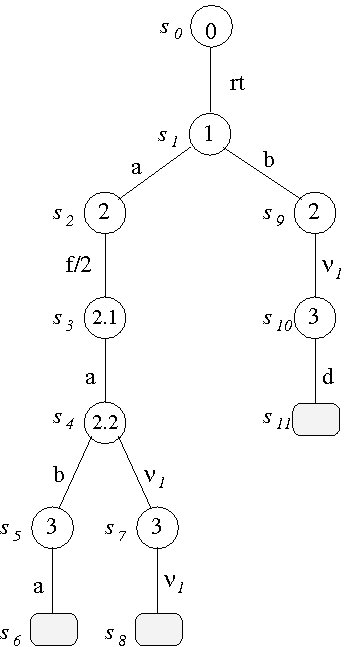
\includegraphics[width=0.3\textwidth]{trie}
%%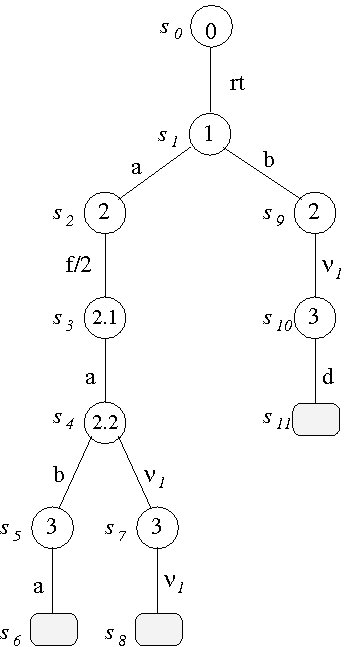
\epsfig{file=trie,height=.3\textheight}
\end{tabular}
\caption{Terms Stored as a Trie}
\end{figure} 
Using a trie for storage has the advantage that discrimination can be
made on a position anywhere in a fact, and directly inserting into or
deleting from a trie is 4-5x faster than with standard dynamic code.
In addition, in trie-dynamic code, there is no distinction between the
index and the code itself, so for many sets of facts trie storage can
use much less space than standard dynamic code.  For instance,
Figure~\ref{fig:trie} shows how the prefix {\tt rt(a,f(a,...} is
shared for the first two facts.  However, trie storage comes with
tradeoffs: first, only facts can be stored in a trie; second, unlike
standard dynamic code, no ordering is preserved among the facts; and
third, duplicate facts are not supported.

In \version{} of XSB, tries that store facts may have the following
forms:
%
\bi
\item {\em General} tries allow arbitrary terms to be inserted in a
  trie.
  %These tries are thread-private so that inserting a term in a
  %  trie $Tr$ in one thread will not be visible to another thread.
  Although such tries are general, they have limitations in memory
  reclamation in \version{} of XSB.  If a term is deleted from $Tr$,
  memory will be reclaimed if it is safe to do so at the time of
  deletion~\footnote{That is, if no choice points are around that may
    cause backtracking into $Tr$.}; otherwise the space will not be
  reclaimed until all terms in $Tr$ are removed by truncating $Tr$.
 %or   until the thread exits.

\item {\em Associative} Associative tries are more restricted
  than general tries: an associative trie combines a {\em key} which
  can be any ground term, with a {\em value} which can be any term.
  Memory for deleted key-value pairs in an associative trie is always
  immediately reclaimed, and insert or delete operations can be faster
  for an associative trie than for a general trie.
  %These tries are private to a thread, and I
  In addition to reclaiming memory when a term is deleted, memory is
  reclaimed when the trie is truncated or dropped.
%, and when the thread exits.

%\item {\em Private, general} tries allow arbitrary terms to be
%  inserted in a trie.  These tries are thread-private so that
%  inserting a term in a trie $Tr$ in one thread will not be visible to
%  another thread.  Although such tries are general, they have
%  limitations in memory reclamation in \version{} of XSB.  If a term
%  is deleted from $Tr$, memory will be reclaimed if it is safe to do
%  so at the time of deletion~\footnote{That is, if no choice points
%    are around that may cause backtracking into $Tr$.}; otherwise the
%  space will not be reclaimed until all terms in $Tr$ are removed by
%  truncating $Tr$ or until the thread exits.
%
%\item {\em Private, associative} Associative tries are more restricted
%  than general tries: an associative trie combines a {\em key} which
%  can be any ground term, with a {\em value} which can be any term.
%  Memory for deleted key-value pairs in an associative trie is always
%  immediately reclaimed, and insert or delete operations can be faster
%  for an associative trie than for a general trie.  These tries are
%  private to a thread, and in addition to reclaiming memory when a
%  term is deleted, memory is reclaimed when the trie is truncated or
%  dropped, and when the thread exits.
%
%\item {\em Shared, associative} tries are associative tries that are
%  shared among threads.  Memory for deleted key-value pairs is always
%  immediately reclaimed, and when the trie is truncated or dropped.
  \ei

\section{Examples of Using Tries}
%
A handle for a trie can be obtained using the {\tt trie\_create/2}
predicate.  Terms can then be inserted into or deleted from that trie,
and terms can be unified with information in the trie, as shown in the
following example:

\begin{example} \rm
First, we create a private general trie: 
{\small
\begin{verbatim}
| ?- trie_create(X,[type(prge)]).
X = 1

yes
\end{verbatim}
}
%
Next, we insert some terms into the trie
{\small
\begin{verbatim}
| ?- trie_insert(1,f(a,b)), trie_insert(1,[a,dog,walks]).

yes
\end{verbatim}
}
Now we can make arbitrary queries against the trie
{\small
\begin{verbatim}
| ?- trie_unify(1,X).

X = [a,dog,walks];

X = f(a,b);

no
\end{verbatim}
}
\noindent
Above, a general query was made, but the query could have been any
Prolog term.  Now we delete a term, and see what's left.
{\small
\begin{verbatim}
| ?- trie_delete(1,f(X,B)).

X = a
B = b

yes
| ?- trie_unify(1,X).

X = [a,dog,walks];

no
\end{verbatim}
}
\end{example}

The behavior of general tries can be contrasted with that of
associative tries as seen in the next example.
\begin{example} \rm
Now we create an associative trie, with abbreviation
{\tt assoc}.
%using the multi-threaded engine
%Now we start by creating a shared associative trie, with abbreviation
%{\tt shas} using the multi-threaded engine
{\small
\begin{verbatim}
| ?- trie_create(X,[type(assoc),alias(foo)]).
X = 1048577

yes
\end{verbatim}
}  \noindent
%
This time we used an alias so now we can use {\tt foo} to refer to
insert a couple of key-value pairs into the trie (we could also use
the trie handle itself) 
{\small
\begin{verbatim}
| ?- trie_insert(foo,pair(sentence(1),[a,dog,walks])), 
     trie_insert(foo,pair(sentence(2),[a,man,snores])).

yes
\end{verbatim}
} \noindent
However, inserting a general term into an associative trie throws an
error
{\small
\begin{verbatim}
| ?- trie_insert(foo,f(a,b)).
++Error[XSB/Runtime/P]: [Domain (f(a,b) not in domain pair/2)]  
in arg 2 of predicate trie_insert/2 
(Inserted term must be key-value pair in trie 1048577)
\end{verbatim}
}  \noindent
Finally, in an associative trie, if we insert a value for a key that
is already in the trie, it will {\em update} the value for that key.
{\small
\begin{verbatim}
| ?- trie_insert(foo,pair(sentence(1),[a,dog,snores])).

yes
| ?- trie_unify(foo,pair(sentence(1),X)).
X = [a,dog,snores]

yes
\end{verbatim}
}

\end{example}

\section{Space Management for Tries}~\label{sec:trie-gc}
%
When creating or adding terms to an interned trie, XSB manages all
space necessary for the terms and their indexes.  However, when
removing a term from a trie an issue may arise if there is a
possibility of backtracking into the term to be removed; this issue
also arises for retracting dynamic code.  In the sequential engine and
in private tries XSB's dynamic clause garbage collector handles space
reclamation when terms are removed from a trie through {\tt
  trie\_delete/2} or similar low-level predicates.  However, in the
case of {\tt trie\_truncate/1} or {\tt trie\_drop/1}, an exception is
thrown if there are active choice points to terms in a trie that is to
be truncated or dropped.

%In the multi-threaded engine the space reclamation problem becomes
%even more difficult for tries that can be shared among threads.  In
%this case, no garbage collection is performed until there is a single
%active thread.  

These space reclamation issues arise for non-associative tries only.
Associative triesessentially contain key-value pairs, and so may have
their space reclaimed upon deletion of a term, or upon truncation or
dropping their trie.
%, regardless of the number of active
%threads~\footnote{Future versions of XSB may extend garbage collection
%  to handle trie truncation, trie dropping and better space
%  reclamation in the multi-threaded engine.}.

\section{Predicates for Tries} 
%
The following subsections describe predicates for inserting terms into
a trie, deleting terms from a trie, and unifying a term with terms in
a trie, predicates for creating, dropping, and truncating tries, as
well as predicates for bulk inserts into and deletes from a trie.
These predicates can apply to any type of trie, and perform full error
checking on their call arguments.  As such, they are safer and more
general than the lower-level trie predicates described in Chapter 1 of
Volume 2 of this manual.  Use of the predicates described here is
recommended for applications unless the need for speed is paramount.

\begin{description}
%
\index{aliases!tries}
\ourmoditem{trie\_create(-TrieId,+OptionList)}{trie\_create/2}{intern}
%
{\tt OptionList} allows optional parameters in the configuration of a
trie to indicate its type and whether an alias should be used.  In the
present version, {\tt OptionList} may contain the following terms
\bi
\item {\tt type(Type)} where {\tt Type} can be one of
\bi
\item {\tt prge} (private, general).
%maintains information that is accessable only to the calling  thread.
  No restrictions are made for accessing information in a private
  trie.
  %In the single-threaded engine, tries are private by default.

\item {\tt pras} (private, associative) creates a private trie that
  maintains key-value pairs in a manner similar to an associative
  array, using the term {\tt pair(Key,Value)}.  Each key must be ground,
  and there may be only one value per key.

%\item {\tt shas} (shared associative) creates a shared trie that
%  maintains key-value pairs in a manner similar to an associative
%  array, using the term {\tt pair(Key,Value)}.  Each key must be
%  ground, and there may be only one value per key.  This option is
%  available only in the multi-threaded engine

%\item {\tt shared(full)} Maintains information that is accessable to
%  all threads, with no restrictions on its access.  In the
%  single-threaded engine, there is no distinction between private and
%  shared tries.
\ei
\item {\tt alias(Alias)}: Allow trie {\tt TrieId} to be referred to
  via {\tt Alias} in all standard trie predicates.  {\tt Alias}
  remains active for {\tt TrieId} until it is dropped.
%
\item {\tt incremental}: Allows tables that depend on trie {\tt
  TrieId} to be automatically updated as information in {\tt TrieId}
  changes (cf. Section~\ref{sec:incr-update-tries}).
%
\item {\tt nonincremental}: Specifies that tables that depend on trie
  {\tt TrieId} should not be automatically updated as information in
  {\tt TrieId} changes (cf. Section~\ref{sec:incr-update-tries}).
\end{itemize}
%
{\bf Error Cases}
\bi
\item 	{\tt TrieId} is not a variable
\bi
\item 	{\tt type\_error(variable,TrieId)}
\ei
\item 	{\tt OptionList} is a partial list or contains an option that is a variable
\bi
\item 	{\tt instantiation\_error}
\ei
\item 	{\tt OptionList} is neither a list nor a partial list
\bi
\item 	{\tt type\_error(list,OptionsList)}
\ei
\item 	{\tt OptionList} contains an option, {\tt Option} not described above
\bi
\item 	{\tt domain\_error(trie\_option,Option)}
\ei
\item An element of {\tt OptionsList} is alias(A) and A is already
  associated with an existing %thread,
  queue, mutex or stream 
\bi
\item {\tt permission\_error(create,alias, A)}
\ei
\item An element of {\tt OptionsList} is alias(A) and A its not an atom
\bi
\item {\tt type\_error(atom,A)}
\ei
\ei
\index{tabling!incremental}

\index{terms!cyclic}
\ourmoditem{trie\_insert(+TrieIdOrAlias,Term)}{trie\_insert/2}{intern}
%
Inserts {\tt Term} into the trie denoted by {\tt TrieIdOrAlias}.  If
{\tt TrieIdOrAlias} denotes an associative trie, {\tt Term} must be of
the form {\tt pair(Key,Value)} where {\tt Key} is ground.  If {\tt
  TrieIdOrAlias} is a general trie and already contains {\tt Term},
the predicate fails (as the same term cannot be inserted multiple
times in the same trie).  Similarly, if {\tt TrieIdOrAlias} is an
associative trie and already contains a value for {\tt Key} the
predicate fails.

Insertion of tries can be controlled by the flags {\tt
  max\_answer\_term\_depth}, {\tt max\_answer\_list\_depth}, {\tt
  max\_answer\_term\_action}, and {\tt max\_answer\_list\_action},
which are also used to control additions of answers to tables.  Using
these flags, if a term to be inserted is cyclic and exceeds a stated
depth, trie insertion may either fail or throw an error depending on
the associated action: see pg. \pageref{prolog-flags}.

{\bf Error Cases}
\bi
\item 	{\tt TrieIdOrAlias} is a variable
\bi
\item 	{\tt instantiation\_error}.
\ei
\item 	{\tt TrieIdOrAlias} is not a trie id or alias
\bi
\item 	{\tt domain\_error(trie\_id\_or\_alias,TrieIdOrAlias)}
\ei
\item 	{\tt TrieIdOrAlias} denotes an associative array, and {\tt Term} 
  does not unify with {\tt pair(\_,\_)} 
\bi
\item 	{\tt domain\_error(pair/2,Term)}
\ei
\item 	{\tt TrieIdOrAlias} denotes an associative array, 
  {\tt Term = pair(Key,Value)} but {\tt Key} is not ground 
\bi
\item 	{\tt misc\_error}
\ei
\item {\tt Key} or {\tt Value} is a cyclic term, or exceeds the depth 
\bi
\item 	{\tt misc\_error}
\ei
\ei
%

\ourmoditem{trie\_unify(+TrieIdOrAlias,Term)}{trie\_unify/2}{intern}
%
Unifies {\tt Term} with a term in the trie denoted by {\tt
  TrieIdOrAlias}.  If {\tt TrieIdOrAlias} denotes a general trie,
successive unifications will succeed upon backtracking.  If {\tt
  TrieIdOrAlias} denotes an associative trie, {\tt Term} must be of
the form {\tt pair(Key,Value)} where {\tt Key} is ground.

{\bf Error Cases}
\bi
\item 	{\tt TrieIdOrAlias} is a variable
\bi
\item 	{\tt instantiation\_error}.
\ei
\item 	{\tt TrieIdOrAlias} is not a trie id or alias
\bi
\item 	{\tt domain\_error(trie\_id\_or\_alias,TrieIdOrAlias)}
\ei
\item 	{\tt TrieIdOrAlias} denotes an associative array, and {\tt Term} 
  does not unify with {\tt pair(\_,\_)} 
\bi
\item 	{\tt domain\_error(pair/2,Term)}
\ei
\item {\tt TrieIdOrAlias} denotes an associative array, 
  {\tt Term = pair(Key,Value)} but {\tt Key} is not ground 
\bi
\item 	{\tt misc\_error}
\ei
\ei

\ourmoditem{trie\_delete(+TrieIdOrAlias,Term)}{trie\_delete/2}{intern}
%
Deletes a term unifying with {\tt Term} from the trie denoted by {\tt
  TrieIdOrAlias}.  {\tt TrieIdOrAlias} denotes a general trie, all
such terms can be deleted upon backtracking.  If {\tt TrieIdOrAlias}
denotes an associative trie, {\tt Term} must be of the form {\tt
  pair(Key,Value)} where {\tt Key} is ground.  In either case, if {\tt
  TrieIdOrAlias} does not contain a term unifying with {\tt Term} the
predicate fails.

{\bf Error Cases}
\bi
\item 	{\tt TrieIdOrAlias} is a variable
\bi
\item 	{\tt instantiation\_error}.
\ei
\item 	{\tt TrieIdOrAlias} is not a trie id or alias
\bi
\item 	{\tt domain\_error(trie\_id\_or\_alias,TrieIdOrAlias)}
\ei
\item 	{\tt TrieIdOrAlias} denotes an associative array, and {\tt Term} 
  does not unify with {\tt pair(\_,\_)} 
\bi
\item 	{\tt domain\_error(pair/2,Term)}
\ei
\item {\tt TrieIdOrAlias} denotes an associative array, 
  {\tt Term = pair(Key,Value)} but {\tt Key} is not ground 
\bi
\item 	{\tt misc\_error}
\ei
\ei
%
\ourmoditem{trie\_truncate(+TrieIdOrAlias)}{trie\_truncate/1}{intern}
%
Removes all terms from {\tt TrieIdOrAlias}, but does not change any of
its properties (e.g. the type of the trie or its aliases).  

@@

{\bf Error Cases}
\bi
\item 	{\tt TrieIdOrAlias} is a variable
\bi
\item 	{\tt instantiation\_error}.
\ei
\item 	{\tt TrieIdOrAlias} is not a trie id or alias
\bi
\item 	{\tt domain\_error(trie\_id\_or\_alias,TrieIdOrAlias)}
\ei
\item There are active failure continuations to terms in {\tt
  TrieIdOrAlias}
\bi
\item 	{\tt miscellaneous\_error}
\ei
\ei

\ourmoditem{trie\_drop(+TrieIdOrAlias)}{trie\_drop/1}{intern}
%
Drops {\tt TrieIdOrAlias}.  {\tt trie\_drop/1} not only removes all
terms from {\tt TrieIdOrAlias}, but also removes information about its
type and any aliases the trie may have.

{\bf Error Cases}
\bi
\item 	{\tt TrieIdOrAlias} is a variable
\bi
\item 	{\tt instantiation\_error}.
\ei
\item 	{\tt TrieIdOrAlias} is not a trie id or alias
\bi
\item 	{\tt domain\_error(trie\_id\_or\_alias,TrieIdOrAlias)}
\ei
\item There are active failure continuations to terms in {\tt
  TrieIdOrAlias}
\bi
\item 	{\tt miscellaneous\_error}
\ei
 \ei

\ourmoditem{trie\_bulk\_insert(+TrieIdOrAlias,+Generator)}{trie\_bulk\_insert/2}{intern}
% 
Used to insert multiple terms into the trie denoted by {\tt
  TrieIdOrAlias}.  {\tt Generator} must be a callable term.  Upon
backtracking through {\tt Generator} its first argument should
successively be instantiated to the terms to be interned in {\tt
  TrieIdOrAlias}.  When inserting many terms into a general trie, {\tt
  trie\_bulk\_insert/2} is faster than repeated calls to {\tt
  trie\_insert/2} as it does not need to make multiple checks that the
choice point stack is free of failure continuations that point into
the {\tt TrieIdOrAlias} trie.  For associative tries, {\tt
  trie\_bulk\_insert/2} can also be faster as it needs to perform
fewer error checks on the arguments of the insert.

\begin{example} \rm
Given the predicate 
\begin{verbatim}
bulk_create(p(One,Two,Three),N):- 
     for(One,1,N),
     for(Two,1,N),
     for(Three,1,N).
\end{verbatim}
and a general trie {\tt Trie}, the goal 
\begin{center}
   {\tt ?- trie\_bulk\_insert(Trie,bulk\_create(\_Term,N))} 
\end{center}
will add $N^3$ terms to {\tt Trie}.
\end{example}

{\bf Error Cases}
\bi
\item 	{\tt TrieIdOrAlias} is a variable
\bi
\item 	{\tt instantiation\_error}.
\ei
\item 	{\tt TrieIdOrAlias} is not a trie id or alias
\bi
\item 	{\tt domain\_error(trie\_id\_or\_alias,TrieIdOrAlias)}
\ei
\item   {\tt Generator} is not a compound term
\bi
\item   {\tt type\_error(compound,Generator)}
\ei
\item 	{\tt TrieIdOrAlias} denotes an associative array, and {\tt Generator} 
  does not unify with {\tt pair(\_,\_)} 
\bi
\item 	{\tt domain\_error(pair/2,Term)}
\ei
\item {\tt TrieIdOrAlias} denotes an associative array, and {\tt
  Generator} succeeds with a term that unifies with {\tt
  pair(Key,Value)} and {\tt Key} is not ground 
\bi
\item 	{\tt misc\_error}
\ei
\item {\tt Key} or {\tt Value} is a cyclic term
\bi
\item 	{\tt misc\_error}
\ei
\ei

\index{terms!cyclic}
\ourmoditem{trie\_bulk\_delete(+TrieIdOrAlias,Term)}{trie\_bulk\_delete/2}{intern}
% 
Deletes all terms that unify with {\tt Term} from {\tt TrieIdOrAlias}.
If {\tt TrieIdOrAlias} denotes an associative trie, the key of the key
value pair need {\em not} be ground.

\begin{example}\label{ex:bulk-delete} \rm
For the trie in the previous example, the goal 
\begin{center}
{\tt ?-  trie\_bulk\_delete(Trie,p(1,\_,\_))} 
\end{center}
will delete the $N^2$ terms that unify with {\tt p(1,\_,\_)} from {\tt TrieIdOrAlias}.
\end{example}

{\bf Error Cases}
\bi
\item 	{\tt TrieIdOrAlias} is a variable
\bi
\item 	{\tt instantiation\_error}.
\ei
\item 	{\tt TrieIdOrAlias} is not a trie id or alias
\bi
\item 	{\tt domain\_error(trie\_id\_or\_alias,TrieIdOrAlias)}
\ei
\ei

\ourmoditem{trie\_bulk\_unify(+TrieIdOrAlias,\#Term,-List)}{trie\_bulk\_unify/3}{intern}
% 
Returns in {\tt List} all terms in {\tt TrieIdOrAlias} that unify with
{\tt Term}.  If {\tt TrieIdOrAlias} denotes an associative trie, the
key of the key value pair need {\em not} be ground.

This predicate is useful for two reasons.  First, it provides a safe
way to backtrack through an associative trie while maintaining the
memory management and concurrency properties of associative tries.
Second, it enforces read consistency for {\tt TrieIdOrAlias},
regardless of whether the trie is private or shared, general or
associative.

\begin{example} \rm
Continuing from Example~\ref{ex:bulk-delete} the goal
\begin{center}
{\tt ?-  trie\_bulk\_unify(Trie,X),List} 
\end{center}
will return the the $N^3 - N^2$ terms still in {\tt TrieIdOrAlias}.
\end{example}

{\bf Error Cases}
\bi
\item 	{\tt TrieIdOrAlias} is a variable
\bi
\item 	{\tt instantiation\_error}.
\ei
\item 	{\tt TrieIdOrAlias} is not a trie id or alias
\bi
\item 	{\tt domain\_error(trie\_id\_or\_alias,TrieIdOrAlias)}
\ei
\item 	{\tt List} is not a variable
\bi
\item 	{\tt type\_error(variable,List)}.
\ei
\ei

\ourmoditem{trie\_property(?TrieOrAlias,?Property)}{trie\_property/2}{intern}
%
If {\tt TrieOrAlias} is instantiated, unifies {\tt Property} with
current properties of the trie; if {\tt TrieOrAlias} is a variable,
backtracks through all the current tries whose properties unify with
{\tt Property}.
%In the MT engine, {\tt thread\_property/2} accesses
%only tries private to the calling thread and shared tries; however
%note that there is no guarantee that that the information returned
%about shared tries will be valid, due to concurrency
%issues~\footnote{{\tt trie\_property/2} is not yet implemented for
%  shared tries.}.

Currently {\tt Property} can have the form 
\bi
\item {\tt type(Type)}: where {\tt Type} is the type of the trie.
%
\item {\tt alias(Alias)}: if the trie has an alias {\tt Alias}
\ei

{\bf Error Cases}
%
\bi
\item {\tt TrieOrAlias} is neither a variable nor an XSB trie id
  nor an alias
\bi
\item {\tt domain\_error(trie, TrieOrAlias)}
\ei
\item {\tt TrieOrAlias} is not associated with a valid trie
\bi
\item {\tt existence\_error(trie, TrieOrAlias)}
\ei
\ei

%\ouritem{trie\_property(+TrieIdOrAlias,Property)}
%\index{\texttt{trie\_property/2}}
%
\end{description}

\section{Low-level Trie Manipulation Utilities}

%The previous sections indicate how tries can be used as an efficient
%mechanism to store thread-private and thread-shared terms.
In this section we describe lower-level trie manipulation predicates
that are suitable for implementing XSB libraries~\footnote{Flora-2,
  XASP, XSB's {\tt storage} library and others use these predicates.}.
As with other tries, these utilities are suitable for storing terms
rather than executable clauses, use a set based semantics, and do not
maintain an ordering among these terms.  In addition
%
\bi
\item These predicates create and maintain
%thread-private,
  general tries.
%
\item These predicates do not always perform error checking.  If not
  explicitly specified in the description of the predicate, errors
  returned may be confusing, and calling with improper arguments may
  even cause memory violations.  
%
\item For historical reasons, the ordering of arguments in these
  predicates is not consistent.
\ei
%
Despite (and sometimes because of) these limitations, the trie
manipulation facilities can be extremely fast, so that interning and
uninterning terms in a trie may be much faster than assert and retract
in XSB or in any other Prolog.

\subsection{A Low-Level API for Interned Tries} \label{sec:intern-basic}
%%
\begin{description}
\ourmoditem{new\_trie(-Root)}{new\_trie/1}{intern} {\tt Root} is
instantiated to a handle for a new private, general trie.


\ourrepeatmoditem{trie\_intern(+Term,+Root)}{trie\_intern/2}{intern}
%
\ourmoditem{trie\_intern(+Term,+Root,-Leaf,-Flag,-Skel)}{trie\_intern/5}{intern}
% 
{\tt trie\_intern/2} effectively asserts \texttt{Term} by interning
into the trie designated by {\tt Root}.  If a variant of {\tt Term} is
already in {\tt Root} the predicate succeeds, but a new copy of {\tt
  Term} is not added to the trie.

{\tt trie\_intern/5} acts as {\tt trie\_intern/2} but returns
additional information: {\tt Leaf} is the handle for the interned {\tt
  Term} in the trie.  {\tt Flag} is 1 if the term is ``old'' (already
exists in the trie); it is 0, if the term is newly inserted.  {\tt
  Skel} represents the collection of all the variables in {\tt
  Term}. It has the form {\tt ret(V1,V2,...,VN)}, exactly as in {\tt
  get\_calls} (see Vol. 1 of the XSB manual).

{\bf Error Cases}
\begin{itemize}
\item 	{\tt Root} is uninstantiated
\bi
\item 	 {\tt instantiation\_error}
\ei
\item 	{\tt Root} is instantiated, but not an integer (trie handle)
\bi
\item 	 {\tt type\_error(integer,Root)}
\ei
\end{itemize}
%%

\ourrepeatmoditem{trie\_interned(?Term,+Root)}{trie\_interned/2}{intern}
%%
\ourmoditem{trie\_interned(?Term,+Root,?Leaf,-Skel)}{trie\_interned/4}{intern}
%%
{\tt trie\_interned/2} backtracks through the terms that unify with
{\tt Term} and that are interned into the trie represented by the
handle {\tt Root}.  {\tt Term} may be free, or partially bound.

If {\tt Leaf} is a free variable, {\tt trie\_interned/5} works as {\tt
  trie\_interned/2}: it backtracks through the terms that unify with
{\tt Term} interned into the trie represented by the handle {\tt
  Root}.  In addition it returns {\tt Leaf} as the handle for each
such term and returns in {\tt Skel} the collection of all the
variables in {\tt Term} using the form {\tt ret(V1,...,Vn)}.
Otherwise, if {\tt Leaf} is bound, {\tt trie\_interned/5} will unify
{\tt Term} with the term in the trie designated by {\tt Leaf}, 
returning a vector of variables in {\tt Skel}.

{\bf Error Cases}
\begin{itemize}
\item 	{\tt Root} is uninstantiated
\bi
\item 	 {\tt instantiation\_error}
\ei
\item 	{\tt Root} is instantiated, but not an integer (trie handle)
\bi
\item 	 {\tt type\_error(integer,Root)}
\ei
\end{itemize}
%%

\ourrepeatmoditem{trie\_unintern(+Root,+Leaf)}{trie\_unintern2}{intern}
\ourmoditem{trie\_unintern\_nr(+Root,+Leaf)}{trie\_unintern\_nr/2}{intern}
%%
{\tt trie\_unintern(+Root,+Leaf)} deletes a term from a trie using the
handle {\tt Leaf}, as obtained from {\tt trie\_intern/[2,4]} or {\tt
  trie\_interned/[2,4]}.  Space is reclaimed for the term only if it
is safe to do so -- if there are no failure continuations that may
consume the term (cf. Section~\ref{sec:trie-gc}).

{\tt trie\_unintern\_nr/2} does not perform space reclamation and as a
result requires no garbage collection -- it simply marks a term as
``deleted''.  This makes {\tt trie\_unintern\_nr/2} suitable if trie
garbage collection may be an issue, and also allows it to be used in
libraries that support backtrackable updates, such as XSB's {\tt
  storage} library.

{\bf Error Cases}
\begin{itemize}
\item 	{\tt Root} or {\tt Leaf} is uninstantiated
\bi
\item 	 {\tt instantiation\_error}
\ei
\item 	{\tt Root} or {\tt Leaf} is instantiated, but not an integer
  (trie handle or trie leaf) 
\bi
\item 	 {\tt type\_error(integer,Root)} or {\tt type\_error(integer,Leaf)}
\ei
\end{itemize}
%%

\ourmoditem{reclaim\_uninterned\_nr(+Root)}{reclaim\_uninterned\_rn/1}{intern}
%%
Runs through the chain of leaves of the trie {\tt Root} and deletes
the terms that have been marked for deletion by {\tt
  trie\_unintern\_nr/2}. This can be viewed either as a garbage
collection step or as a commit.

{\bf Error Cases}
\begin{itemize}
\item 	{\tt Root} is uninstantiated
\bi
\item 	 {\tt instantiation\_error}
\ei
\item 	{\tt Root} is instantiated, but not an integer (trie handle)
\bi
\item 	 {\tt type\_error(integer,Root)}
\ei
\end{itemize}
\ourmoditem{unmark\_uninterned\_nr(+Root,+Leaf)}{unmark\_uninterned\_nr/2}{intern}
The term pointed to by {\tt Leaf} should have been previously marked
for deletion using {\tt trie\_unintern\_nr/2}. This term is then
``unmarked'' (or undeleted) and becomes again a normal interned term.

{\bf Error Cases}
\begin{itemize}
\item 	{\tt Root} or {\tt Leaf} is uninstantiated
\bi
\item 	 {\tt instantiation\_error}
\ei
\item 	{\tt Root} or {\tt Leaf} is instantiated, but not an integer
  (trie handle or trie leaf) 
\bi
\item 	 {\tt type\_error(integer,Root)} or {\tt type\_error(integer,Leaf)}
\ei
\end{itemize}
%%
\ourmoditem{delete\_trie(+Root)}{delete\_trie/1}{intern} 
%%
Deletes all the terms in the trie pointed to by {\tt Root}.  Garbage
collection ensures that space reclamation is performed only if it is
safe to do so.

{\bf Error Cases}
\begin{itemize}
\item 	{\tt Root} is uninstantiated
\bi
\item 	 {\tt instantiation\_error}
\ei
\item 	{\tt Root} is instantiated, but not an integer (trie handle)
\bi
\item 	 {\tt type\_error(integer,Root)}
\ei
\item 	Failure continuations point to one or more nodes in the trie with root {\tt Root}
\bi
\item 	{\tt misc\_error}
\ei
\end{itemize}
%%

\end{description}

\index{tries!interned|)}

\chapter{Hooks} \label{hooks}

Sometimes it is useful to let the user application catch certain
events that occur during XSB execution. For instance, when the user
asserts or retracts a clause, etc.  XSB has a general mechanism by
which the user program can register \emph{hooks} to handle certain
supported events. All the predicates described below must be imported
from {\tt xsb\_hook}.


\section{Adding and Removing Hooks}

A hook in XSB can be either a 0-ary predicate or a unary predicate.
A 0-ary hook is called without parameters and unary hooks are called with
one parameter. The nature of the parameter depends on the type of the hook,
as described in the next subsection.


\begin{description}
\ourmoditem{add\_xsb\_hook(+HookSpec)}{add\_xsb\_hook/1}{xsb\_hook}

This predicate registers a hook; it must be imported from {\tt xsb\_hook}.
{\tt HookSpec} has the following format:
%%
\begin{quote}
 {\tt
   hook-type(your-hook-predicate(\_))
   }
\end{quote}
%%
or, if it is a 0-ary hook:
%%
\begin{quote}
  {\tt
   hook-type(your-hook-predicate)
   }  
\end{quote}
%%
For instance, 
%%
\begin{verbatim}
    :- add_xsb_hook(xsb_assert_hook(foobar(_))).
\end{verbatim}
%%
registers the hook {\tt foobar/1} as a hook to be called when XSB
asserts a clause. Your program must include
clauses that define {\tt foobar/1}, or else an error will result.

The predicate that defines the hook type must be imported from {\tt
  xsb\_hook}:
%%
\begin{verbatim}
    :- import xsb_assert_hook/1 from xsb_hook.  
\end{verbatim}
%%
or {\tt add\_xsb\_hook/1} will issue an error.

\ourmoditem{remove\_xsb\_hook(+HookSpec)}{remove\_xsb\_hook/1}{xsb\_hook}

Unregisters the specified XSB hook; imported from {\tt xsb\_hook}. For
instance,
%%
\begin{verbatim}
    :- remove_xsb_hook(xsb_assert_hook(foobar(_))).
\end{verbatim}
%%
As before, the predicate that defines the hook type must be imported from
{\tt xsb\_hook}.
\end{description}


\section{Hooks Supported by XSB}

The following predicates define the hook types supported by XSB. They must
be imported from {\tt xsb\_hook}.

\begin{description}
\ourmoditem{xsb\_exit\_hook(\_)}{xsb\_exit\_hook/1}{xsb\_hook} 

These hooks are called just before XSB exits. You can register as many
hooks as you want and all of them will be called on exit (but the order of
the calls is not guaranteed). Exit hooks are all 0-ary and must be registered
as such:
%%
\begin{verbatim}
    :- add_xsb_hook(xsb_exit_hook(my_own_exit_hook)).
\end{verbatim}
%%


\ourmoditem{xsb\_assert\_hook(\_)}{xsb\_assert\_hook/1}{xsb\_hook} 
%
These hooks are called whenever the program asserts a clause. An assert
hook must be a unary predicate, which expects the clause
being asserted as a parameter. For instance,
%%
\begin{verbatim}
    :- add_xsb_hook(xsb_assert_hook(my_assert_hook(_))).
\end{verbatim}
%%
registers {\tt my\_assert\_hook/1} as an assert hook. One can register
several assert hooks and all of them will be called (but the order is
not guaranteed).  After the assert\_hooks are called, the original
assert will be called to add the clause to the database.

\ourmoditem{xsb\_intercept\_assert\_hook(\_)}{xsb\_intercept\_assert\_hook/1}{xsb\_hook} 
%
These hooks are called whenever the program asserts a clause.  (They
are called after all xsb\_assert\_hooks, if any, are called.)  An
intercept\_assert hook must be a unary predicate, which expects a
length 2 list as a parameter.  The first element of the list is the
clause being asserted; the second element is 1 for assert (and
assertz), or 0 for asserta.  For instance,
%%
\begin{verbatim}
:- add_xsb_hook(xsb_intercept_assert_hook(my_intercept_assert_hook(_))).
\end{verbatim}
%%
registers {\tt my\_intercept\_assert\_hook/1} as an intercept\_assert
hook. One can register several intercept\_assert hooks and the first
one that succeeds will apply (the order is not guaranteed).  If any
call to an intercept\_assert\_hook succeeds, then the assert is {\em not}
invoked, so it is expected that the intercepting hook will assert any
desired clause.  If no call to the hook predicate succeeds, then the
assert is invoked.  This allows a user, for example, to re-direct all
asserts to one predicate to another different predicate.

\ourmoditem{xsb\_retract\_hook(\_)}{xsb\_retract\_hook/1}{xsb\_hook} 
%
These hooks are called whenever the program retracts a clause, using
{\tt retract/1} or {\tt retractall/1}. A retract hook must be a unary
predicate, which expects as a parameter a list of the form {\tt
  [Head,Body]}, which represent the head and the body parts of the
clause being retracted. As with assert hooks, any number of retract
hooks can be registered and all of them will be called in some order.
After the retract\_hook has been called, the original retract (or
retractall) is called to perform the retraction.

\ourmoditem{xsb\_intercept\_retractall\_hook(\_)}{xsb\_intercept\_retractall\_hook/1}{xsb\_hook} 
%
These hooks are called whenever the program calls {\tt retractall/1}
on a term.  (They are called after all xsb\_retract\_hooks, if any,
are called.)  An intercept\_retractall hook must be a unary predicate,
which expects the term passed to {\tt retractall/1} as a
parameter. For instance,
%%
\begin{verbatim}
:- add_xsb_hook(xsb_intercept_retractall_hook(my_intercept_retractall_hook(_))).
\end{verbatim}
%%
registers {\tt my\_intercept\_retractall\_hook/1} as an intercept\_retractall
hook. One can register several intercept\_retractall hooks and the first
one that succeeds will apply (the order is not guaranteed).  If any
call to an intercept\_retractall\_hook succeeds, then the retractall is {\em not}
invoked, so it is expected that the intercepting hook will retractall any
desired clause(s).

\end{description}


%%% Local Variables: 
%%% mode: latex
%%% TeX-master: "manual1"
%%% End: 

\chapter{Debugging and Profiling} \label{debugging}
%====================================
\index{debugger}
\index{tracing|(}
\section{Prolog-style Tracing and Debugging}
%===========================
\index{tracing!Prolog programs}
%
XSB supports a version of the Byrd four-port debugger for interactive
debugging and tracing of Prolog code.  In this release (\version), it
does not work very well when debugging code involving tabled
predicates~\footnote{The current version of XSB's Prolog debugger does
  not include exceptions as a debugging port.}.  If one only creeps
(see below), the tracing can provide some useful information.  For
programs that involve large amounts of tabling forest-view tracing can
be used (Section~\ref{sec:forest-trace}).
To turn on tracing, use {\tt trace/0}, {\tt trace/1}, or {\tt trace/2}.  To
turn tracing off, use {\tt notrace/0}.

\begin{description}
\repeatstandarditem{trace}{trace/0}
\standarditem{notrace}{notrace/0}

When tracing is on, the system will print a message each time a
predicate is:
\begin{enumerate} \index{debugger!ports}
\item initially entered (Call), 
\item successfully returned from (Exit), 
\item failed back into (Redo), and
\item completely failed out of (Fail).  
\end{enumerate}
When debugging interactively, a message may be printed and tracer
stopped and prompts for input.  (See the predicates {\tt show/1} and
{\tt leash/1} described below to modify what is traced and when the
user is prompted.)

In addition to single-step tracing, the user can set spy points to
influence how the tracing/debugging works.  A spy point is set using
{\tt spy/1}.  Spy points can be used to cause the system to enter the
tracer when a particular predicate is entered. Also the tracer allows
``leaping'' from spy point to spy point during the debugging process.
%
The debugger also has profiling capabilities, which can measure the cpu
time spent in each call. The cpu time is measured only down to 0.0001-th
of a second.

When the tracer prompts for input, the user may enter a return, or a single
character followed by a return, with the following meanings:
\bi
\index{trace!options}
\item{\tt c, <CR>}: {\em Creep}~ Causes the system to single-step to
  the next port (i.e.\ either the entry to a traced predicate called
  by the executed clause, or the success or failure exit from that
  clause).
\item{\tt a}: {\em Abort}~ \index{abort!trace facility} Causes execution to abort
  and control to return to the top level interpreter.
\index{break level}
\item{\tt b}: {\em Break}~ Calls the evaluable predicate {\em break},
  thus invoking recursively a new incarnation of the system
  interpreter.  The command prompt at break level $n$ is
  \begin{center}
    {\tt $n$: \tt ?-}
  \end{center}
  The user may return to the previous break level by entering the system
  end-of-file character (e.g.\ {\tt ctrl-D}), or typing in the atom 
  {\tt end\_of\_file}; or to the top level interpreter by typing in
  {\tt abort}.
\item{\tt f}: {\em Fail}~ Causes execution to fail, thus transferring
  control to the Fail port of the current execution.
\item{\tt h}: {\em Help}~ Displays the table of debugging options.
\item{\tt l}: {\em Leap}~ Causes the system to resume running the
  program, only stopping when a spy-point is reached or the program
  terminates.  This allows the user to follow the execution at a
  higher level than exhaustive tracing.
\item{\tt n}: {\em Nodebug}~ Turns off debug mode.
\item{\tt r}: {\em Retry (fail)}~ Transfers to the Call port of the current
  goal.  Note, however, that side effects, such as database modifications
  etc., are not undone.
\item{\tt s}: {\em Skip}~ Causes tracing to be turned off for the entire
  execution of the procedure.  Thus, nothing is seen until control comes
  back to that procedure, either at the Success or the Failure port.
\item{\tt q}: {\em Quasi-skip} This is like Skip except that it does not mask
  out spy points.
\item{\tt S}: {\em Verbose skip}~ Similar to {\tt Skip} mode, but trace
  continues to be printed. The user is prompted again when the current call
  terminates with success or failure.  This can be used to obtain a full
  trace to the point where an error occurred or for code profiling. (See
  more about profiling below.)
\item{\tt e}: {\em Exit}~ Causes immediate exit from \ourprolog\ back to the
  operating system.
\ei
%/* TLS: it seems like there may not be much use for the non-queryable trace/1 */

\standarditem{trace(+Filename,+option)}{trace/2}
\index{trace!logging}
%\index[pred]{\texttt{trace/1}}
%\index{\texttt{trace/1}}
%
{\tt trace/2} is like {\tt trace/0} except that it is non-interactive
and dumps trace information into a log file, {\tt Filename}.
Currently the only supported option is \texttt{log}.  However, the log
is written in the form of Prolog facts, which can be loaded
queried. The format of the facts is:
%% 
\begin{verbatim}
xsb_tracelog(CallId,CallNum,PortType,ParentCallNum,DepthOfCall,CurrentCall,Time)
\end{verbatim}
%% 
where \texttt{CallId} is an identifier generated when XSB encounters a
new top-level call. This identifier remains the same for all subgoals
called while tracing that top-level call.
\bi
\item \texttt{CallNum} is a generated number to show the nesting of
  the calls being traced. It is the same number that the user sees
  when tracing interactively.
%
\item \texttt{PortType} is \texttt{'Call'}, \texttt{'Redo'},
  \texttt{'Exit'}, or \texttt{'Fail'}.  
\item \texttt{ParentCallNum} is the call number of the parent call.
%
\item \texttt{DepthOfCall} is the nesting depth of the current call
  with respect to its ancestor calls.  
%
\item \texttt{CurrentCall} is the call being traced
%
\item \texttt{Time} is the CPU time it took to execute
  \texttt{CurrentCall}. On \texttt{'Call'} and \texttt{'Redo'},
  \texttt{Time} is always 0 --- it has a meaningful value only for the
  \texttt{'Exit'} and \texttt{'Fail'} log entries. 
\end{itemize}
It should be noted that when calls are delayed due to the well-founded
negation computation of because of the \texttt{when/2} primitive, the
parent call might be off in some cases. However, the parent property
repairs itself for subsequent calls.

`The name of the predicate (\texttt{xsb\_tracelog}) used for logging
can be changed by asserting it into the predicate
\texttt{debug\_tracelog\_predicate/1}, which should be imported from
\texttt{usermod}. For instance,
%% 
\begin{verbatim}
   :- import debug_tracelog_predicate/1 from usermod.
   ?- assert(debug_tracelog_predicate(foobar)).
\end{verbatim}
%% 

\standarditem{spy(Preds)}{spy/1}
    where {\tt Preds} is a spy specification or a list of such
    specifications, and must be instantiated. This predicate sets spy
    points (conditional or unconditional) on predicates.  A spy
    specification can be of several forms. Most simply, it is a term
    of the form $P$/$N$, where $P$ is a predicate name and $N$ its
    arity.  Optionally, only a predicate name can be provided, in
    which case it refers to all predicates of any arity currently
    defined in {\tt usermod}.  It may optionally be prefixed by a
    module name, e.g.  $ModName$:$P$/$N$. (Again, if the arity is
    omitted, the specification refers to all predicates of any arity
    with the given name currently defined in the given module.)  A spy
    specification may also indicate a conditional spy point. A
    conditional spy specification is a Prolog rule, the head
    indicating the predicate to spy, and the body indicating
    conditions under which to spy. For example, to spy the predicate
    p/2 when the first argument is not a variable, one would write:
    $spy (p(X,\_):-nonvar(X)).$ (Notice that the parentheses around
    the rule are necessary). The body may be empty, i.e., the rule may
    just be a fact.  The head of a rule may also be prefixed (using
    $:$) with a module name. One should not put both conditional and
    unconditional spy points on the same predicate.

\standarditem{nospy(Preds)}{nospy/1}
    where {\tt Preds} is a spy specification, or a list of such
    specifications, and must be instantiated at the time of call.  What
    constitutes a spy specification is described above under {\tt spy}.
    {\tt nospy} removes spy points on the specified predicates. If a
    specification is given in the form of a fact, all conditional spy points
    whose heads match that fact are removed.

\standarditem{debug}{debug/0}
    Turns on debugging mode.
    This causes subsequent execution of predicates with trace or spy
    points to be traced, and is a no-op if there are no such predicates.
    The predicates {\tt trace/0}, {\tt trace/1}, \texttt{trace/2},  and {\tt spy/1} cause debugging mode
    to be turned on automatically.

\standarditem{nodebug}{nodebug/0}
    Turns off debugging mode.  This causes trace and spy points to be ignored.

\standarditem{debugging}{debugging/0}
    Displays information about whether debug mode is on or not, and lists
    predicates that have trace points or spy points set on them.

\standarditem{debug\_ctl(option,value)}{debug\_ctl/2}
   {\tt debug\_ctl/2} performs debugger control functions as described below.
   These commands can be entered before starting a trace or inside the trace.
   The latter can be done by responding with ``{\tt b}'' at the prompt,
   which recursively invokes an XSB sub-session. At this point, you can
   enter the debugger control commands and type \verb|end_of_file.| This
   returns XSB back to the debugger prompt, but with new settings.
   %%
   \begin{enumerate}
   \item {\tt debug\_ctl(prompt, off)} Set non-interactive mode globally.
     This means that trace will be printed from start to end, and the user
     will never be prompted during the trace.
    \item {\tt debug\_ctl(prompt, on)} 
      Make tracing/spying interactive.
    \item {\tt debug\_ctl(profile, on)}  
      Turns profiling on. This means that each time a call execution
      reaches the {\tt Fail} or {\tt Exit} port, CPU time spent in that
      call will be printed. The actual call can be identified by locating a
      {\tt Call}  prompt that has the same number as the ``cpu time''
      message.
    \item {\tt debug\_ctl(profile, off)}  
      Turns profiling off.
    \item {\tt debug\_ctl(redirect, +File)} 
      Redirects debugging output to a file. This also includes program output,
      errors and warnings.
      Note that usually you cannot see the contents of {\tt +File} until it
      is closed, {\it i.e.}, until another redirect operation is performed
      (usually {\tt debug\_ctl(redirect, tty)}, see next).
    \item {\tt debug\_ctl(redirect, tty)}     
      Attaches the previously redirected debugging, error, program output,
      and warning streams back to the user terminal.
    \item {\tt debug\_ctl(show, +PortList)}  
      Allows the user to specify at which ports should trace messages be
      printed. {\tt PortList} must be a list of port names, i.e., a sublist
      of ['Call', 'Exit', 'Redo', 'Fail']. 
    \item {\tt debug\_ctl(leash, +PortList)}  
      Allows the user to specify at which ports the tracer should stop
      and prompt the user for direction.  {\tt PortList} must be a list of
      port names, i.e., a sublist of ['Call', 'Exit', 'Redo', 'Fail'].  Only
      ports that are {\tt show}-n can be {\tt leash}-ed. 
    \item {\tt debug\_ctl(hide, +PredArityPairList)}  
      The list must be of the form {\tt [P1/A1, P2/A2, ...]}, {\it i.e.},
      each either must specify a predicate-arity pair. Each predicate on
      the list will become non-traceable. That is, during the trace, each
      such predicate will be treated as an black-box procedure, and trace
      will not go into it.
    \item {\tt debug\_ctl(unhide, ?PredArityPairList)} If the list is a
      predicate-arity list, every predicate on that list will become
      traceable again. Items in the list can contain variables. For
      instance, {\tt debug\_ctl(unhide, [\_/2])} will make all 2-ary that
      were previously made untraceable traceable again.  As a special case,
      if {\tt PredArityPairList} is a variable, all predicates previously
      placed on the ``untraceable''-list will be taken off.
    \item {\tt debug\_ctl(hidden, -List)}
      This returns the list of predicates that the user said should not be
      traced.
   \end{enumerate}
   %%
\end{description}


\subsection{Control of Prolog-Style Tracing and Debugging}
%--------------------------------------------------
\index{tracing!Prolog program!controls}
%
\index{low-level tracing} \index{tracing!low-level}

XSB debugger also provides means for the low-level control of what
must be traced. Normally, various standard predicates are masked out
from the trace, since these predicates do not make sense to the
application programmer.  However, if tracing below the application
level is needed, you can retract some of the facts specified in the
file {\tt syslib/debugger\_data.P} (and in some cases assert into
them). All these predicates are documented in the header of that
file. Here we only mention the four predicates that an XSB developer
is more likely to need. To get more trace, you should retract from the
first three predicates and assert into the last one.
%%
\begin{itemize}
\item {\tt hide\_this\_show(Pred,Arity)}: specifies calls (predicate name and
  arity) that the debugger should {\tt not} show at the prompt. However,
  the evaluation of this hidden call {\tt is} traced.
\item {\tt hide\_this\_hide(Pred,Arity)}: specifies calls to hide. Trace
  remains off while evaluating those predicates. Once trace is off, there
  is no way to resume it until the hidden predicate exits or fails.
\item  {\tt show\_this\_hide(Pred,Arity)}: calls to show at the
  prompt. However, trace is switched off right after that.
\item  {\tt trace\_standard\_predicate(Pred,Arity)}: Normally trace doesn't
  go inside standard predicates ({\it i.e.}, those specified in
  {\tt syslib/std\_xsb.P}. If you need to trace some of those, you must
  {\tt assert} into this predicate.
\end{itemize}
%%
In principle, by retracting all facts from the first three predicates and
asserting enough facts into the last one, it is possible to achieve the
behavior that approximates the {\tt -T} option. However, unlike {\tt -T},
debugging can be done interactively. This does not obviate {\tt -T},
however. First, it is easier to use {\tt -T} than to issue multiple asserts
and retracts. Second, {\tt -T} can be used when the error occurs early on,
before the moment when XSB shows its first prompt.

Finally, XSB also provides a facility for low-level tracing of Prolog
execution.  This can be activated by invoking the emulator with the
{\tt -T} option (see Section~\ref{sec:EmuOptions}), or through the
predicate {\tt trace/0}.  \stdrefindex{\$trace/0} It causes trace
information to be printed out at {\em every} Prolog call (including
those to system predicates, and tabled predicates).  While this method
can occasionally be useful, its use is limited.  For tabled executions
the techniques in the following sections are much more appropriate.
Ever for Prolog programs, the volume of such trace information can become
very large very quickly, so this method of tracing is only recommended
for situations where no other debugging method is useful.

%-----------------------------------------------------------------------------
\newcommand{\ctrace}{{\tt logforest}}

\section{Trace-based Execution Analysis through Forest Logging} \label{sec:forest-trace}
%
The tracing and debugging described in previous sections has proven
useful for Prolog programs for 30 or more years.  However, when
tabling is added to Prolog, things change.  First, as described in
Chapter~\ref{chap:TablingOverview}, tabling can be used to find the
least fixed point of mutually recursive predicates.  Operationally,
this requires the ability to suspend one computation path and to
resume another.  Second, the addition of tabled negation for the
well-founded semantics requires the ability to delay negative goals
whose only proof may be involved in a loop through negation and to
simplify these goals once their truth value has become
known. Furthermore, a tabled subgoal has different states: it may be
{\em new}; it may be {\em incomplete} so that new answers might be
derived for it; or {\em completed} (completely evaluated) so that the
answers may simply be read from the table.  In short, tabling, which
can execute much more general programs than Prolog and which can use
the stronger well-founded semantics, requires a more complex set of
operations than Prolog's SLDNF.  Accordingly, debugging and tracing
is correspondingly more complex.  Thus, while Prolog's 4-port debugger
may be useful for programs that involve just a few tabled predicates,
it may not be useful for programs that heavily use tabling for complex
recursions, non-monotonic reasoning or other purposes.

There is currently no standard approach to debugging tabled programs.
One possible approach would be to extend the 4-port debugger to
include other ports for tabling operations.  Such extensions have not
yet been explored, and whether the paradigm of n-port debugging can be
extended to full tabling so that it can be useful to programmers is an
open question.  Another approach would be use the declarative approach
of {\em justification} \cite{GuRR01,PGDRR04} to explain why
derivations were or were not made.  XSB does in fact have a
justification package but it is not currently robust enough to be
recommended for general use.  Below we present the {\tt \ctrace}
approach~\cite{Swif14b}

\subsection{Tracing a tabled evaluation through forest logging}
%
While the operations used for tabling are more complex than those of
SLDNF, they have a clear formal operational semantics through SLG and
the forest-of-trees model.  We recall this model briefly below for a
definite program but assume a background knowledge of tabled logic
programming (see, for instance~\cite{SwiW12}).

\begin{example} \rm 
Figure~\ref{fig:local} shows a program fragment along with an SLG
forest for the query {\tt ?- reach(1,Y)} to the the right-recursive
tabled predicate {\tt reach/1}.  An SLG forest consists of an SLG tree
for each tabled subgoal $S$: this tree has root $S \mif{} S$.  In a
definite program an SLG tree represents resolution of program clauses
and answers to prove $S$.  In Figure~\ref{fig:local} each non-root
node of the form $K. N$ where $N = (S \mif{} Goals)\theta$ is a clause
in which the bindings to a subgoal $S$ are maintained in $S\theta$,
the goals remaining to prove $S$ are in $Goals\theta$, and the order
of creation of $N$ within the tabled evaluation is represented by a
number, $K$ (local scheduling is used in this example).  Children of a
root node are obtained through resolution of a tabled subgoal against
program clauses.  Children of non-root nodes are obtained through
answer clause resolution, if the left most selected literal is tabled
(e.g. children of node 3 or 11 in the tree for {\tt reach(1,Y)}), or
through program clause resolution if the leftmost selected literal is
not tabled (e.g. children of nodes 2 and 18 in the tree for {\tt
  reach(1,Y)}).  Nodes that have empty {\em Goals} are termed {\em
  answers}.
%
\begin{figure}[htbp]
\centering
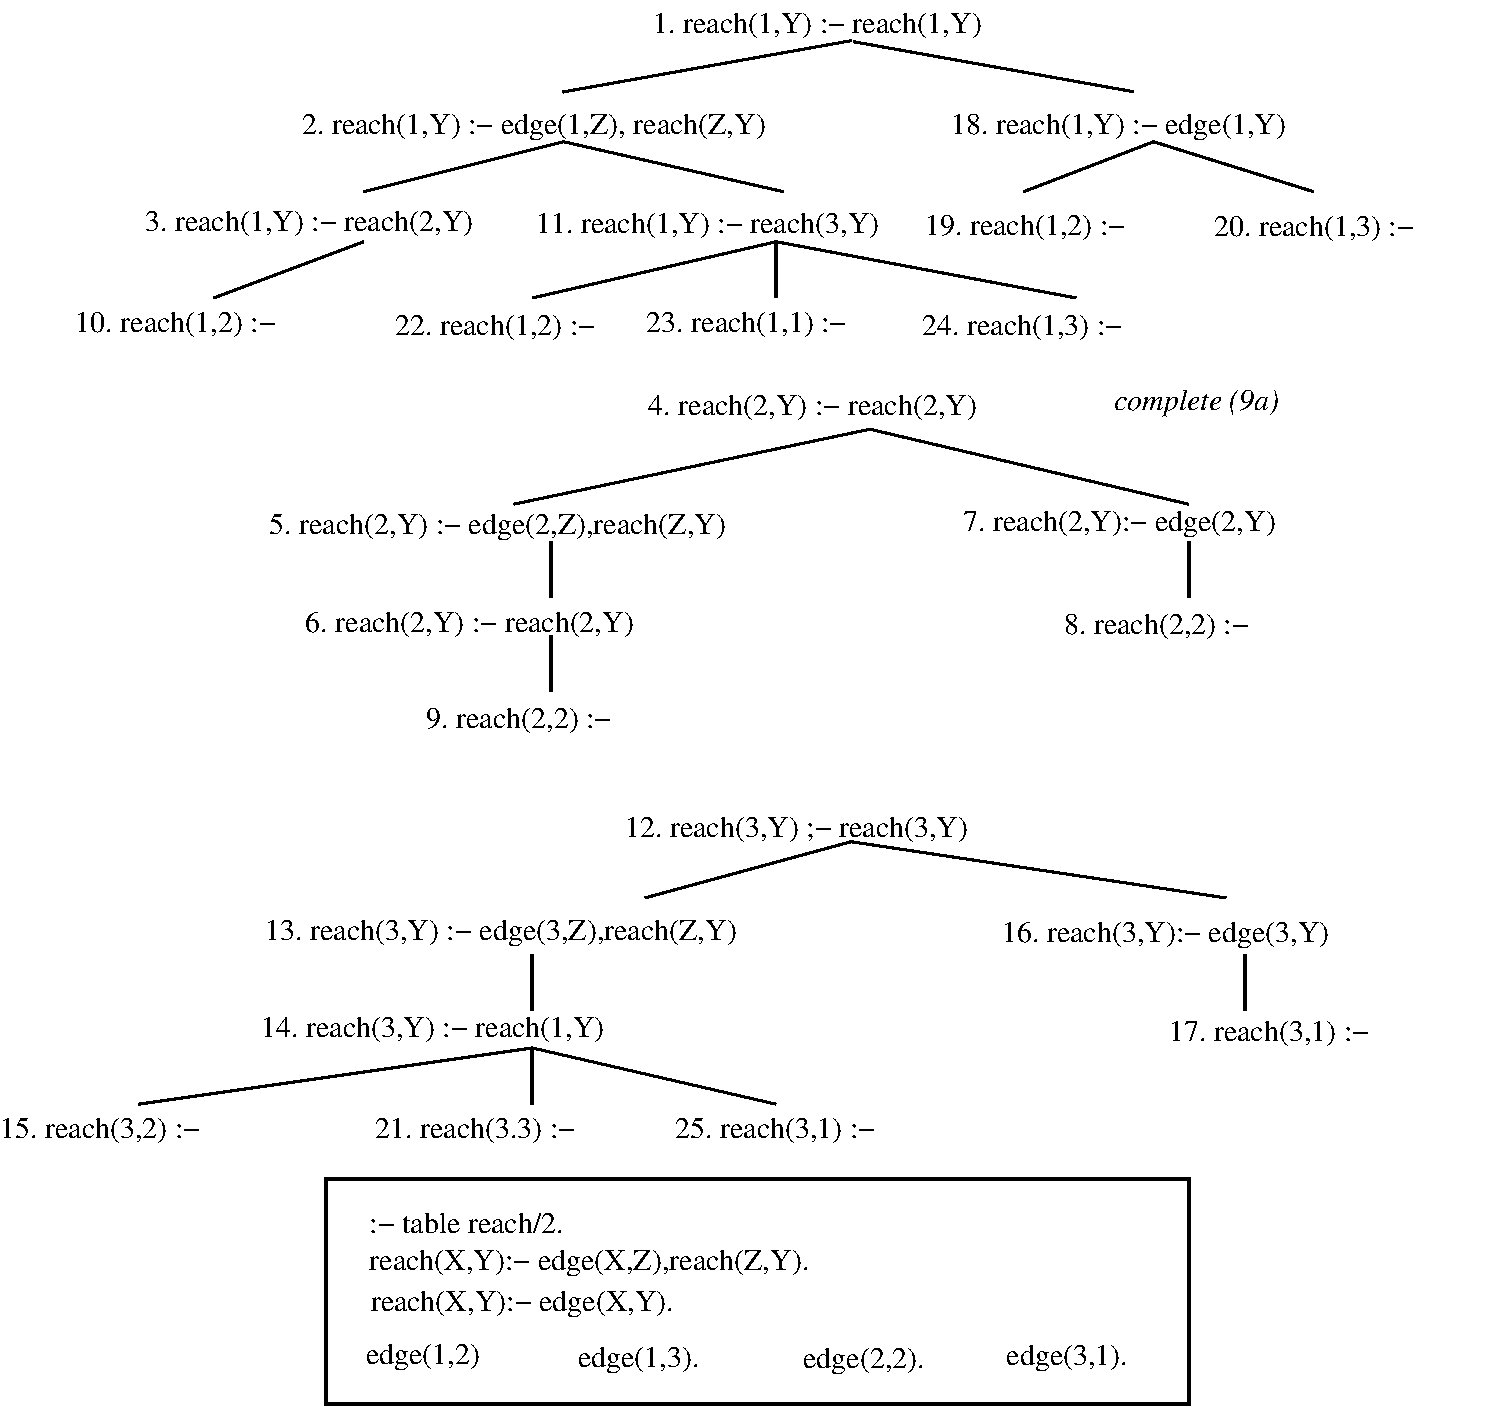
\includegraphics[width=.99\textwidth]{slg-forest-local}
%%\mbox{
%%{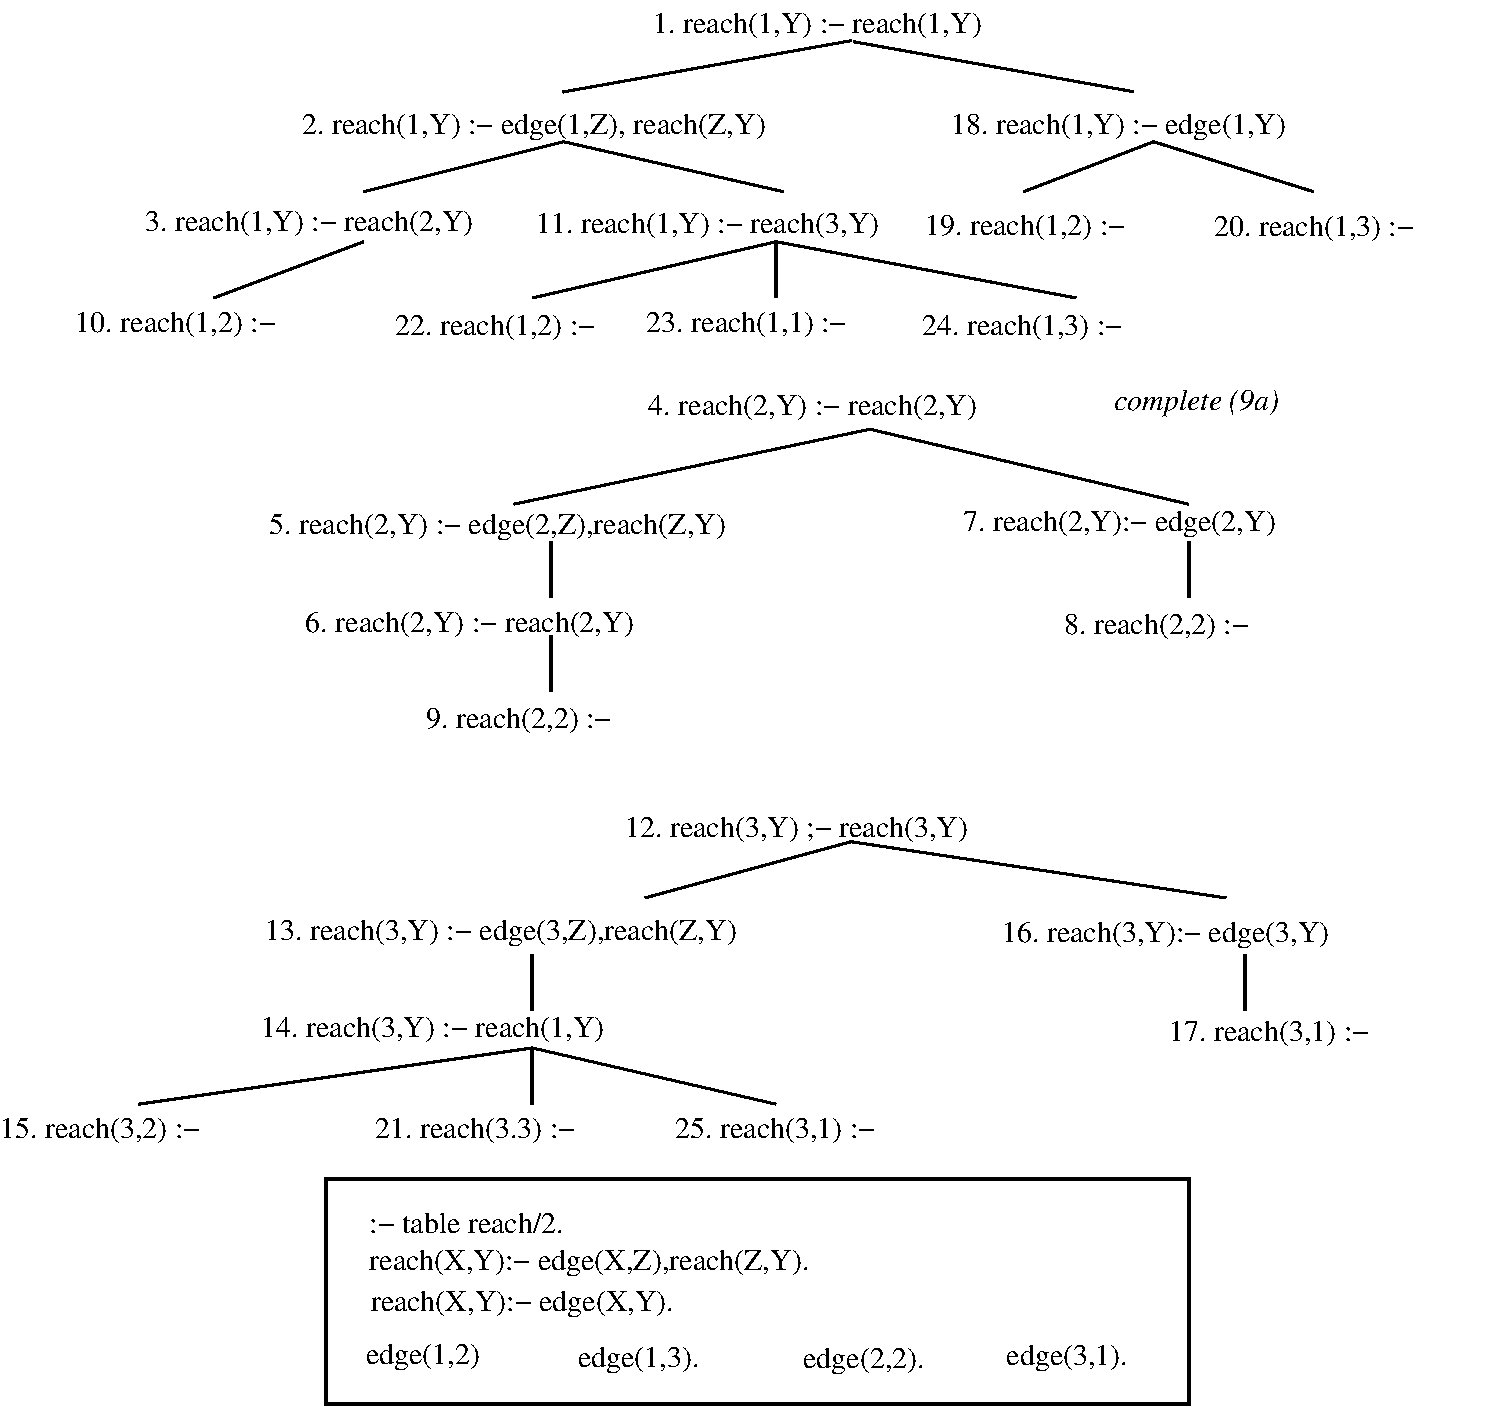
\epsfig{file=slg-forest-local,width=.99\textwidth}}}
\caption{A program $P_{Rrec}$ and SLG forest for (local) evaluation of
  {\tt ?- reach(1,Y)}} \label{fig:local}
\end{figure}
%
Note that the evaluation keeps track of each tabled subgoal $S$ that
it encounters.  Later if $S$ is selected again, resolution will use
answers rather than program clauses; if no answers are available, the
computation will {\em suspend} at that point and the evaluation will
backtrack to try to derive answers using some other computation path.
Once more answers have been derived, the evaluation {\em resumes} the
suspended computation.  Similarly, once the computation has
backtracked through all answers available for $S$ in the current
state, the computation path will suspend, and resume after further
answers are found.  Thus a tabled evaluation is a fixed point
computation for a set of interdependent subgoals.  When it is
determined that a (perhaps singleton) set of subgoals can produce no
more answers, the subgoals are completed.
\end{example}

%\vspace{0.1in}

The forest logging approach ({\tt \ctrace}) allows one to run a tabled
query and produce a log that can be interpreted as (a partial image
of) an SLG forest.  The log can then used to analyze program
correctness, to optimize performance and so on.  Because \ctrace{}
  produces a log, it superficially resembles the non-interactive trace
  described earlier in this chapter.  However,
\begin{itemize}
\item {\tt trace/1} produces a Prolog-style trace that takes little
  account of tabling.  \ctrace{} structures its output according to
  the forest-of-trees model, and takes little account of program
  clause resolution.

\item \ctrace{} is implemented in C for efficiency, while {\tt
  trace/1} is built on top of XSBs interactive debugger.  Unlike {\tt
  trace/1}, \ctrace{} can therefore to produce logs for very large
  evaluations with little overhead.
\end{itemize}

Currently, \ctrace{} captures the following actions.

\bi
\item {\em A call to a tabled subgoal}~ If a positive call to a tabled
  subgoal $S_1$ is made from a tree for $S_2$ a Prolog-readable fact
  of the form {\tt tc(S1,S2,Stage,Counter)} is logged, where {\em
    Counter} is the ordinal number of the fact, and {\tt Stage} is
\bi
\item {\tt new} if $S_1$ is a new subgoal
\item {\tt cmp} if $S_1$ is not a new subgoal and has been completed
\item {\tt incmp} if $S_1$ is not a new subgoal but has {\em not} been
  completed 
\item {\tt reeval} if $S_1$ is an incremental subgoal being re-evaluated.
\ei 
%
If the call is negative a fact of the form {\tt
  nc(S1,S2,Stage,Counter)} is logged, where all arguments are as
above.

  For instance, in the above example, node 3 would be represented as
  {\tt tc(reach(2,Y),reach(1,Y),2)} (the reason for using the counter
  value of 2 rather than 3 is explained below).  If $S_1$ is the first
  tabled subgoal in an evaluation, $S_2$ is the atom {\em null}.

\item {\em Derivation of a new answer}~ When a new {\em unconditional}
  answer $A$ is derived for subgoal $S$ and added to the table
  (i.e. $A$ is not already an answer for $S$) a fact of the form {\tt
    na(A,S,Counter)} is logged.  In the above example, the answer node
  9 would be represented as {\tt na([2],reach(2,\_v1),4)} where the
  first argument is a list of substitutions for the variables {\em
    \_v1,...,\_vn} in $S$.

  When a new {\em conditional} answer $A \mif D|$, with substitution
  $A$ and delayed literals $D$. is derived for subgoal $S$ and added
  to the table a fact of the form {\tt nda(A,S,D,Counter)} is logged.

\item {\em Return of an answer to a consuming subgoal}~When an
  unconditional answer $A$ is returned to a consuming subgoal $S$ in a
  tree for $S_T$, a fact of the form {\tt ar(A,S,ST,Counter)} is
  logged.  A log entry is made only if the table for $S$ is incomplete
  (see the explanation below).

  If the answer $A$ is conditional, the fact has the form {\tt
    dar(A,S,ST,Counter)}, where each argument is as above.

\item {\em Delaying a selected negative literal}.  If a selected
  negative literal $L$ of a node $N$ is delayed, because it is
  involved in a loop through negation, and $N$ is in a tree for $S_T$,
  a fact of the form {\tt dly(L,$S_T$,Counter)} is logged.

\index{strongly connected components (SCCs)}
\item {\em Subgoal completion}
\bi
\item When a set $\cS$ of subgoals is determined to be completely
  evaluated and is completed, a fact of the form {\tt
    cmp(S,SCCNum,Counter)} is logged for each $S \in \cS$.  Here
  $SCCNum$ is simply a number giving an ordinal value that can be used
  to group subgoals into mutually dependent sets of subgoals (here
  called {\em Strongly Connected Components} or {\em SCCs}), i.e. the
  {\em SCCNum} of each $S \in \cS$ has the same value, but that value
  is not used for a completion fact of any subgoal not in $\cS$.
%
\index{tabling!early completion of subgoals}
\item When a subgoal $\cS$ is {\em early completed}, i.e. it is
  determined that no more answers for $S$ are possible or are desired
  a fact of the form {\tt cmp(S,ec,Counter)} is logged.  If $S$
  belonged to a larger mutually dependent set $\cS$ when it was early
  completed, $S$ will also be included in the completion facts for
  $\cS$.  \ei
\item {\em Table Abolishes}
\bi
\item When a tabled subgoal $S$ is abolished, a fact of the form {\tt
  ta(subg(S),Counter)} is logged.
\item When all tables for a predicate $p/n$ are abolished, a fact of
  the form {\tt ta(pred(p/n),Counter)} is logged.
\item When all tables are abolished, a fact of the form {\tt ta(all,Counter)} is logged.
\ei
%
\item {\em Location of errors} Whenever an error is thrown and the
  execution is in a tree for a subgoal $S$, a Prolog-readable fact of
  the form {\tt err(S,Counter)} is logged, where {\em Counter} is the
  ordinal number of the fact.  The primary purpose of this fact is to
  indicate the nearest tabled call that gave rise to an uncaughterror.  \ei

{\tt logforest} does {\em not} contain

\bi
\item Information about the occurrence of program clause resolution
  either when used to produce children of tabled predicates, or when
  it is used to produce children whose nodes have a selected literal
  that is non-tabled.

\item Information about the return of answers from completed tables.
  XSB uses a so-called {\em completed table optimization} which treats
  answer return from completed tables in a manner akin to program
  clause resolution.  
 \ei

\index{attributed variables}
\noindent
The inclusion of the above two features in {\tt logforest} would
significantly slow down execution of XSB.  However, future versions of
{\tt logforest} may include expanded logging features for negation,
for call and answer subsumption and for incremental
tabling~\footnote{Currently, attributes of attributed variables are
  not printed out.}.

\begin{example}
The forest for {\tt reach(1,Y)} in the foregoing example has the log
file as shown in Table~\ref{tab:fview}.

\begin{table}[htbp]
\begin{tabular}{lll}               \\ \hline  
Log File                                     & Forest & Explanation\\ \hline 
tc(reach( 1,\_v0),null,new,0)                & node 1 & \\
                                             & node 2 & created by program clause resol. \\
                                             & node 3 & created by program clause resol. \\
tc(reach( 2,\_v0),reach( 1,\_v0),new,1)      & node 4 & \\
                                             & node 5 & created by program clause resol.\\
                                             & node 6 & created by program clause resol. \\
tc(reach( 2,\_v0),reach( 2,\_v0),incmp,2)    &        & repeated subgoal registered\\
                                             & node 7 & created by program clause resol. \\
                                             & node 8 & created by program clause resol. \\
na([ 2],reach( 2,\_v0),3)                    & node 8 & registered as answer\\
ar([ 2],reach( 2,\_v0),reach( 2,\_v0),4)     & node 9 & created by answer resol.\\
cmp(reach( 2,\_v0),2,5)                      &    9a   & {\tt reach(2,\_v0)} completed \\
                                             & node 10 & created by return from completed table \\
na([ 2],reach( 1,\_v0),6)                    & node 10 & registered as an answer\\
                                             & node 11 & created by program clause resol. \\
tc(reach( 3,\_v0),reach( 1,\_v0),new,7)      & node 12 & \\
                                             & node 13 & created by program clause resol. \\
                                             & node 14 & created by program clause resol. \\
tc(reach( 1,\_v0),reach( 3,\_v0),incmp,8)    & node 14 & repeated subgoal registered \\
ar([ 2],reach( 1,\_v0),reach( 3,\_v0),9)     & node 15 & created by answer resol. \\
na([ 2],reach( 3,\_v0),10)                   & node 15 & registered as an answer \\
                                             & node 16 & created by program clause resol. \\
                                             & node 17 & created by program clause resol. \\
na([ 1],reach( 3,\_v0),11)                   & node 17 & registered as an answer \\
                                             & node 18 & created by program clause resol. \\
                                             & node 19 & created by program clause resol. (repeated answer)\\
                                             & node 20 & created by program clause resol.\\
na([ 3],reach( 1,\_v0),12)                   & node 20 & registered as an answer\\
ar([ 3],reach( 1,\_v0),reach( 3,\_v0),13)    & node 21 & created by answer return\\
na([ 3],reach( 3,\_v0),14)                   & node 21 & registered as an answer\\
ar([ 2],reach( 3,\_v0),reach( 1,\_v0),15)    & node 22 & created by answer resol.\\
ar([ 1],reach( 3,\_v0),reach( 1,\_v0),16)    & node 23 & created by answer resol.\\
na([ 1],reach( 1,\_v0),17)                   & node 23 & registered as an answer \\
ar([ 3],reach( 3,\_v0),reach( 1,\_v0),18)    & node 24 & created by answer resol. \\
ar([ 1],reach( 1,\_v0),reach( 3,\_v0),19)    & node 25 & created by answer resol.v \\
cmp(reach( 1,\_v0),1,20)                     &  & \\
cmp(reach( 3,\_v0),1,21)   & & \\ \hline
\end{tabular}
\caption{Log file for computation in Figure~\ref{fig:local}}\label{tab:fview}
\end{table}
\end{example}

\begin{description}
\ourrepeatmoditem{log\_forest(+Call)}{log\_forest/2}{tables}
\ourmoditem{log\_forest(+Call,+Options)}{log\_forest/2}{tables}
%
These predicates turn on forest logging, call {\tt Call}, then turn
logging off when {\tt Call} is finished.  {\tt Options} is a list of
possible options.
%
\bi
\item {\tt Options} may contain the term {\tt file(File)} which directs
  the logging to {\tt File}; otherwise the log will be sent to
  standard output.
\item {\tt Options} may contain the term {\tt level(Level)} where {\tt
  Level} may be one of the following values.
\bi
\item {\tt full} which means that all tabling actions are logged as
  described above.
%
\item {\tt partial} which means that answer return operations are not
  logged.
%
\item {\tt calls\_only} which does not log  answer return, new
  answer, nor simplification operations.
\ei 
%
The levels {\tt partial} and {\tt calls\_only} both reduce the size of
  the log which can be useful for analyzing some computations.
%
\item {\tt Options} may contain the term {\tt
  set\_pred(PredSpec,Mode)} where {\tt Mode} is {\tt on} or {\tt off}.
  This allows certain predicates not to be logged, a useful feature if
  only part of a program needs to be debugged
\ei

{\bf Error Cases} 
\bi
\item {\tt Options} is a variable, or contains a variable as an element
\bi
\item {\tt instantiation\_error}
\ei
\item {\tt Options} is not a list
\bi
\item {\tt type\_error(list,Options)}
\ei
\item {\tt Options} contains an option {\tt O} that is not a forest
  logging option.  
\bi
\item {\tt domain\_error(forest\_logging\_option,O)}
\ei
\ei


\index{indexing}
\ourmoditem{load\_forest\_log(+File)}{load\_forest\_log/1}{tables}
%
The log produced by {\tt log\_forest/[1,2]} is a Prolog file that can
be compiled and/or loaded dynamically just as any other Prolog file.
However, for large logs (i.e. those of many megabytes) use of {\tt
  load\_dync/[1,2]} XSB commands can drastically reduce the time
needed to load the file, while use of the proper {\tt index/2}
declarations can greately improve query time.  The simple predicate,
{\tt load\_forest\_log/1} loads a log file and indexes needed arguments.
\end{description}

\index{tracing|)}

\subsection{Analyzing the log; seeing the forest through the trees} \label{sec:forest-log-anal}
%
As previously described, forest logging is based on the formal
operational semantics of SLG, and as a result the log can be analyzed
to query any result that can be modeled by the theory.  But despite
the power of forest logging, it can be difficult to use.  Not all
users have the background to fully understand the operational
semantics of SLG.  Even those users with a formal background may find
it difficult to write efficient analysis routines for logs of large
computations~\footnote{I find it difficult myself!}.  Accordingly, XSB
provides routines that analyze logs and display information about a
computation.  These routines can answer many questions about a
computation and can provide the starting point for further
exploration.  We introduce these routines via an extended example.

\begin{example} \rm \label{ex:scc-anal}
%
This example arises from the actual use of forest logging to
understand a Flora-2 computation~\cite{YaKZ05}, in which the Cyc
reasoner (cf. http://www.cyc.com) was translated into Silk
(cf. http://silk.semwebcentral.org) and used to answer various
questions in biology.  Silk itself compiles into Flora-2 which in turn
compiles into XSB~\footnote{This example was run in 2012 using a
  64-bit server with a large amount of RAM.}.  After translation,
query answering took more resources than expected, and users wanted to
determine why.  Using the features of \version{}, the first step is to
call {\tt statistics/0} at the end of the computation.  The statistics
indicated that the computation took about 30 seconds of CPU time and
300 megabytes of table space, while XSB's trail had allocated over 1
gigabyte of space.  The call to {\tt statistics/0} also showed the
following information:
%
\begin{verbatim}
  8678944 variant call check/insert ops: 615067 producers, 8063877 variants.
  317346 answer check/insert ops: 304899 unique inserts, 12447 redundant.
\end{verbatim}
In other words, there were nearly 10 million tabled subgoals that were
called, indicating that this computation was heavily tabled (a
characteristic of most Flora-2 computations), It also shows that the
average number of answers per tabled subgoal is rather small.

This basic information leads to several questions.  Why were there so
many tabled subgoals?  Did the tabling have anything to do with the
large amount of choice-point/trail space that was allocated?  Which
tabled subgoals had answers?  How many times did a given tabled
predicate call another tabled predicate?

\predref{table\_dump/2} \predref{table\_dump/3} Some of
these questions can be answered by {\tt table\_dump/[2,3]}:
particularly, what tabled subgoals were called, and which had answers.
However {\tt table\_dump/[2,3]} cannot provide other information, such
as the dependencies of given tabled subgoals on other tabled subgoals
or the order in which operations occurred.  From a formal perspective,
{\tt table\_dump/[2,3]} does not allow a user to analyze an entire SLG
forest: only the ``table'', i.e., the subgoals in the forest and the
unordered set of its answers.  The table omits any information about
interior nodes or completion information, both of which are used to
compute dependency information.  Dependencies are useful in analyzing
most computations, but is especially important in Flora-2 computations
such as this one, that make heavy use of HiLog.  This use of HiLog
means that the dependencies of tabled predicates on one another is not
at all obvious, and may not easily be determined by static analysis.

The next step, therefore, in analyzing this computation is to rerun it
with forest logging.  For this computation forest logging has no
impact on memory usage, but increases the time of the computation from
about 30 seconds to about 52 seconds --- around 73\% in this case.  It
is worthwhile noting that the actual overhead of forest logging varies
depending on how heavily the computation is tabled.  The log itself
had slightly over 14 million entries which were loaded into XSB via
{\tt load\_forest\_log/1}.  The log took about 140 seconds to load and
about 7.8 Gbytes of space for the log facts and their multiple and
trie indexes~\footnote{The load time for this example, about 100,000
  facts/second is typical for 2012 CPUs; the size of the loaded code
  is larger than usual, due in part to the expansion in the size of
  terms caused by the HiLog encoding.}.

The easiest way to start the analysis is to ask the query {\tt ?-
  forest\_log\_overview}, which for this example gives:
%
\begin{verbatim}
There were 613496 subgoals in 463330 (completed) SCCs.  
93918 subgoals were early-completed.  
0 subgoals were not completed in the log.
There were a total of 8670043 tabled subgoal calls:
    613496 were calls to new subgoals
    4467747 were calls to incomplete subgoals
    3588800 were calls to complete subgoals

Number of SCCs with 1 subgoals is 463322
Number of SCCs with 4 subgoals is 1
Number of SCCs with 7 subgoals is 1
Number of SCCs with 52 subgoals is 1
Number of SCCs with 110 subgoals is 4
Number of SCCs with 149671 subgoals is 1
\end{verbatim}
%
\index{tabling!complete evaluation}
\index{tabling!early completion of subgoals} 
%
The overview extends the information shown by {\tt
  statistics/0}.  First, the total number of completed and
non-completed SCCs is given along with a count of how many of the
completed subgoals were early completed.  Information about
non-completed SCCs is useful, since the forest log may be analyzed for
a computation that does not terminate.  Since this computation did
terminate, all subgoals in the log were completed~\footnote{The slight
  difference between the number of subgoals shown here and the number
  shown by {\tt statistics/0} is due to the use of tabling in the
  Flora compiler.}.  Note that there is also a breakdown of calls to
tabled subgoals that distinguishes whether the tabled subgoal was new,
completed, or incomplete.  Recall that calls to completed tabled
subgoals essentially treat the answers in the table as facts, so that
these calls are efficient.  Making a call to an incomplete subgoals on
the other hand means that the calling and called subgoals are mutually
recursive~\footnote{This statement is true in local evaluation but not
  in batched evaluation.} and execution of recursive sets of subgoals
can be expensive, especially in terms of space.

Finally, the overview report provides the distributions of tabled
subgoals across SCCs.  While most of the SCCs were small there was a
large one, with nearly 150,000 mutually dependent subgoals.  Clearly
the large SCC should be examined.  The first step is to obtain its
index.  The query
%
\begin{verbatim}
get_scc_size(SCC,Index)), Index > 1000.
\end{verbatim}
%
returns the information that the index of the large SCC was 39.  The
query {\tt analyze\_an\_scc(39,userout)} then provides the following
information.
%
\begin{verbatim}
There are 149671 subgoals and 4461290 links (average of 30.8073 edges per subgoal) 
      within the SCC

There are 2 subgoals in the SCC for the predicate backchainForbidden / 0
There are 2 subgoals in the SCC for the predicate 
                   http://www.cyc.com/silk/implementation/transformationPredicate / 0
:
There are 15613 subgoals in the SCC for the predicate gpLookupSentence / 3
There are 15613 subgoals in the SCC for the predicate removalSentence / 3
There are 18770 subgoals in the SCC for the predicate forwardSentence / 3
There are 18771 subgoals in the SCC for the predicate lookupSentence / 3

Calls from assertedSentence/3 to lookupSentence/3 : 32
Calls from backchainForbidden/0 to 'http://www.cyc.com/silk/implementation/transformationPredicate'/0 : 2
:
Calls from transformationSentence/2 to sbhlSentence/3 : 5479
Calls from tvaSentence/3 to removalSentence/3 : 7695
\end{verbatim}
%
It is evident from the first line in this report that the vast
majority of the calls to incomplete tables during this computation
occur in the SCC under investigation.  Since information on incomplete
tables is kept in XSB's choice point stack (cf. \cite{SaSw98}), the
evaluation of SCC 39 is the likely culprit behind the large amount of
stack space required.  The subgoals in the SCC are first broken out by
their predicate name and arity, then the edges within the SCC are
broken out by the predicates of their caller and called subgoals.  At
this point a programmer can review the various rules for {\tt
  lookupSentence/3}, {\tt forwardSentence/3} and other predicates to
determine whether the recursion is intended and if so, whether it can
be simplified.
%
\end{example}

\subsubsection{Using abstraction in the analysis}
%
Within the SCC analysis, information about a given tabled subgoal $S$
was abstracted to the functor and arity of $S$.  For this example,
abstraction was necessary, as reporting 150,000 subgoals or 4,000,000+
would not provide useful information for a human being.  However, it
could be the case that seeing the tabled subgoals themselves would be
useful for a smaller SCC.  Even for an SCC of this size, different
levels of abstraction could be useful: mode information or type
information might be useful in a given circumstance.  

\begin{example} \label{ex:moded-scc-anal} \rm
%
Making the call {\tt ?-
  analyze\_an\_scc(39,userout,abstract\_modes(\_,\_))} applies the
predicate {\tt abstract\_modes/2} to each term, producing an output of
the form:
%
\begin{verbatim}
There are 149671 subgoals and 4461290 links (average of 30.8073 edges per subgoal) 
           within the SCC

There are 3 subgoals in the SCC for the predicate backchainRequired(g,g)
There are 2 subgoals in the SCC for the predicate backchainForbidden(g,g)
:
There are 29254 subgoals in the SCC for the predicate gpLookupSentence(g,g)
There are 29254 subgoals in the SCC for the predicate removalSentence(g,g)

Calls from assertedSentence(g,g) to lookupSentence(g,g) : 10
Calls from assertedSentence(m,g) to lookupSentence(m,g) : 22
:
Calls from transformationSentence(m,g) to sbhlSentence(m,g) : 741
Calls from tvaSentence(g,g) to removalSentence(g,g) : 7695
\end{verbatim}
%
{\tt abstract\_modes(In,Out)} simply goes through each argument of
{\tt In} and unifies the corresponding argument of {\tt Out} with a
{\tt v} if the argument is a variable, a {\tt g} if the argument is
ground, and {\tt m} otherwise.  

\end{example}
%
{\tt abstract\_modes/2} is simply an example: any term-abstraction
predicate may be passed into the last argument of {\tt
  analyze\_an\_scc/3}~\footnote{Because of the special representation
  of Flora-2 terms, abstraction was used to produce the output of
  Example~\ref{ex:moded-scc-anal}, while a more sophisticated version
  of {\tt abstract\_modes/2} was used in
  Example~\ref{ex:moded-scc-anal}.}.

\subsubsection{Analyzing Negation}
%
Many programs that use negation are stratified in such a way that they
do not require the use of {\sc Delaying} and {\sc Simplification}
operations, and the routines described in the previous section are
sufficient for these programs.  However if a program does not have a
two-valued well-founded model, a user would often like to understand
why.  Even in a program that is two-valued, the heavy use of {\sc
  Delaying} and {\sc Simplification} can indicate that some rules may
need to be optimized by having their literals reordered.

\begin{example} \label{ex:neg} \rm
Figure~\ref{fig:neg} shows a program with negation and illustrates SLG
resolution for the query {\em p(c)} to the program.  The nodes in
Figure~\ref{fig:neg} have been annotated with the order in which they
were created under local scheduling. In the formalism used by
Figure~\ref{fig:neg}, the symbol $|$ in a node separates the
unresolved goals to the right from the delayed goals to the left.  In
the evaluation state where nodes 1 through 10 have been created, {\em
  p(b)} has been completed, and {\em p(a)} and {\em p(c)} are in the
same SCC.  There are no more clauses or answers to resolve, but {\em
  p(a)} is involved in a loop through negation in node 5, and nodes 2
and 10 involve {\em p(a)} and {\em p(c)} in a negative
loop~\footnote{In this example, we ignore the effects of early
  completion which would complete {\em p(b)} immediately upon creation
  of node 8, obviating the need to create node 9.}.

In situations such as this, where all resolution has been performed
for nodes in an SCC, an evaluation may have to apply a {\sc Delaying}
operation to a negative literal such as {\em not(p(a))}, in order to
explore whether other literals to its right might fail. 
% In cases such as this, 
When multiple literals can be delayed, an arbitrary one is chosen to
be delayed first.  So the evaluation delays the selected literal of
node 2 to generate node 12 producing a {\em conditional answer} -- an
answer with a non-empty delay list
(cf. Section~\ref{sec:conditional-answers} for an overview of how XSB
computes and allows inspection of delayed literals).  Next, {\em not
  p(a)} in node 5 is delayed, failing that computation path, and {\em
  not p(c)} in node 10 is delayed to produce node 15 and failing the
final computation path for {\em p(a)}.  At this stage the SCC
$\{p(a),p(c)\}$ is {\em completely evaluated} meaning that there are
no more operations applicable for goal literals (as opposed to delay
literals).  Since {\em p(a)} is completely evaluated with no answers,
conditional or otherwise, the evaluation determines it to be {\em
  failed} and a {\sc Simplification} operation can be applied to the
conditional answer of node 12, leading to the {\em unconditional}
answer in node 17 and {\em success} of the literal {\em p(c)}.
\end{example}

\begin{figure*}[tbp] 
\begin{center}
%\fbox{\epsfig{file=Figures/del-simpl3.eps,width=\textwidth}}
\epsfig{file=del-simpl3.eps,width=\textwidth}
\end{center}
\caption{A Normal Program and SLG Forest for Evaluation of the Query {\em p(c)}}
\label{fig:neg}
\end{figure*}


As indicated previously, the forest log overview includes a total
count of {\sc Delaying} and {\sc Simplification} operations, as well
as a count of conditional answers.  In addition, SCC analysis counts
negative as well as positive links within the SCC.  The current
version of forest logging also provides a means to examine the causes
of answers that have an undefined truth value.  Recall from
Example~\ref{ex:neg} that there are two types of causes of an
undefined truth value: either 1) a negative literal explicitly
undergoes a {\sc Delaying} operation; or 2) a conditional answer may
be used to resolve a literal.  It can be shown that in local
evaluation, a conditional answer $A$ will never be returned out of an
SCC if $A$ is successful or failed in the well-founded model of a
program.  This means that if an answer for $S$ is undefined, then it
would be caused operationally by a {\sc Delaying} operation within the
SCC of $S$ or within some other SCC on which $S$ depends.  So to
understand why an atom is undefined it can be useful understand the
``root causes'' of the delay: to examine SCCs in which {\sc Delaying}
operations were executed and conditional answers were derived, but the
answers could not be simplified.
% into unconditional answers.

\begin{example}
As a use case, logging was made of execution of a Flora-2 program that
tested out a new defeasibility theory.  The forest log overview
indicated that the top-level query was undefined: 
%
\begin{small}
\begin{verbatim}
:
There were a total of 55 negative delays
There were a total of 0 simplifications
There were a total of 695 unconditional answers derived:
There were a total of 66 conditional answers derived:
\end{verbatim}
\end{small}
%
The analysis predicate {\tt three\_valued\_scc(List)} produces a list
of all SCC indices in which {\sc Delaying} caused the derivation of
conditional answers.  These SCCs can then be analyzed as discussed in
the previous section.
\end{example}

\subsection{Discussion}
%
Using log forest imposes a relatively minimal overhead on most
computations, considering the information it can provide, and loading
and analysis is relatively quick.  For this example, the top level
analysis took around 10 seconds, and analysing SCC 39 took about 20
seconds in Example~\ref{ex:scc-anal} and about 60 seconds in
Example~\ref{ex:moded-scc-anal}.  For more information,
see~\cite{Swif14b}.

\subsection{Predicates for Forest Logging}

\begin{description}
\ourmoditem{forest\_log\_overview}{forest\_log\_overview/0}{tables}
%
Provides an overview of subgoals, calls, and SCCs in the forest log as
indicated in Section~\ref{sec:forest-log-anal}.

\ourmoditem{get\_scc\_size(?Index,?Size)}{get\_scc\_size/3}{tables}
%
This simple predicate determines the indices of SCCs whose size is
{\tt Size}, for use with {\tt analyze\_an\_scc/[2,3]}.

\ourmoditem{three\_valued\_sccs(List)}{three\_valued\_scc/1}{tables}
%
If there are any SCCs in the log where delay is performed, causing
conditional answers to be added that were not simplified into
unconditional answers, unifies {\tt List} with the index of all such
SCCs.

\ourrepeatmoditem{analyze\_an\_scc(+Index,+File)}{analyze\_an\_scc/2}{tables}
\ourmoditem{analyze\_an\_scc(+Index,+File,+Abstraction)}{analyze\_an\_scc/3}{tables}
%
These predicates can be used to analyze the SCC indexed by {\tt Index}
in a forest log, as explained in Section~\ref{sec:forest-log-anal}.
The output is written to {\tt File}; calling the predicate with {\tt
  File} set to {\tt userout} causes the output to be written to the
console.  In {\tt analyze\_an\_scc/2}, tabled subgoals are abstracted
to predicate indicators, in {\tt analyze\_an\_scc/3}, a two-ary
abstraction predicate in {\tt usermod} is called.

Error conditions on {\tt File} are the same as {\tt tell/1}.

\ourmoditem{abstract\_modes(Term,AbstractedTerm)}{abstract\_modes/2}{usermod}
%
{\tt abstract\_modes(In,Out)} simply goes through each argument of
{\tt Term} and unifies the corresponding argument of {\tt Abstracted}
with a {\tt v} if the argument is a variable, a {\tt g} if the
argument is ground, and {\tt m} otherwise.

To use this predicate, the file {\tt term\_abstract.P} must be loaded,
via {\tt ensure\_loaded/1} or similar means.

\ourmoditem{set\_forest\_logging\_for\_pred(+PredSpec,+Mode)}{set\_forest\_logging\_for\_pred/2}{tables}
If forest logging is active, this predicate allows any logging
specific to the predicate or term indicator, {\tt PredSpec}, to be
turned on or off.  Thus, for instance, tabled predicates in a
pre-existing library need not clutter up the log.

{\bf Error Cases}
\bi
\item 	{\tt PredSpec} is not a predicate or term indicator.
\bi
\item 	{\tt type\_error}
\ei
%
\item 	{\tt Mode} is not in the set \{{\tt on},{\tt off}\}
\bi
\item 	{\tt domain\_error}
\ei
\ei
\end{description}

%%% Local Variables: 
%%% mode: latex
%%% TeX-master: "manual1"
%%% End: 

%-----------------------------------------------------------------------------

\section{Inspecting a Tabled Derivation} \label{sec:suspend-analyze}

As described in the previous section, Forest Logging is a powerful
technique for understanding the operational aspects of a tabled
derivation, and is based on the idea that a derivation is itself a
mathematical entity that can be represented and analyzed.  This basis
allows Forest Logging to support various types of analysis including
profiling the derivation, and understanding its termination
properties~\cite{LiaK13,LiaK13a}.  At the same time, Forest Logging
may not always be convenient to use.  Since it is a trace-based
analysis a (sometimes very large) trace file must be created and
loaded before being analyzed.

An alternate approach is to use {\em inspection predicates} -- a term
that loosely refers to predicates useful for understanding a tabled
derivation.  Most of these predicates can be used in two ways.  First,
they can inspect an on-going derivation that has been suspended
through various means.  Alternately, they may be used to retroactively
inspect a derivation that has completed.  In this section, we first
describe two important sets of interactive inspection predicates.
First we describe the {\tt table\_dump} library which provides a
flexible approach to inspecting tables
(Section~\ref{sec:table-dump}).\footnote{Other predicates for table
  inspection that are generally lower-level are described in
  Section~\ref{sec:TablingPredicates}.}  Next we discuss a set of
predicates for inspecting various dependency graphs of a computation
(Section~\ref{sec:dep-graph}.  We then discuss how {\em tripwires} can
automatically suspend a derivation for inspection at a point where the
derivation begins to use too many resources, and so might be
inefficient (Section~\ref{sec:tripwire}).

\subsection{Inspecting Tables with {\tt table\_dump}} \label{sec:table-dump}

\begin{description}
\ourrepeatmoditem{table\_dump(+Term,+OptionList)}{table\_dump/2}{dump\_table}
%
\ourmoditem{table\_dump(+Stream,\#Term,+OptionList)}{table\_dump/3}{dump\_table}
%
{\tt table\_dump/[2,3]} provides an easy method to view subgoals and
answers that are present in a table.  Given an input {\tt Term}, {\tt
  table\_dump/[2,3]} provides information about all tabled subgoals
that are subsumed by {\tt Term}; if {\tt Term} is a variable,
information is provided about all tables.

The information can be provided at three levels of aggregation, and
the form of the information is determined by the options in {\tt
  OptionsList}.
%
\begin{itemize}
\item If the option {\tt summary(true)} is set, the aggregate sum
  of subgoals and answers that are subsumed by {\tt Term} is
  collected, along with the aggregate sum of calls {\it to} these
  subgoals.  If {\tt Term} is a variable this information is broken
  down by tabled predicates.
%
\begin{itemize}
\item If {\tt details(answers)} is set, a list is collected of every
  tabled subgoal $S$ such that $S$ is subsumed by {\tt Term} along
  with the number of answers for each $S$ along with a list of those
  answers and the truth value of each answer ({\tt t} if true and {\tt
    u} if undefined).  If {\tt Term} is a variable this information is
  broken down by tabled predicates.
%
\item If {\tt details(subgoals)} is set, a list is collected of all
  subgoals $S$ such that $S$ is subsumed by {\tt Term} along with the
  number of answers for each $S$.  However, unlike the action for {\tt
    details(answers)} the actual list of answers for $S$ is not
  returned.  If {\tt Term} is a variable this information is broken
  down by tabled predicates.
%
\item If {\tt details(false)} is set, no detail information is
  provided for the actual subgoals or their answers.
\end{itemize}
%
\item If {\tt OptionsList} contains the option {\tt results(X)} for
  some variable {\tt X}, {\tt X} will be instantiated upon
  backtracking to all information collected about the tables.
%
\item If the option {\tt output(true)} is set, the information is
  written to {\tt Stream} or to {\tt userout} in Prolog-readable form.
\end{itemize}
%
If not otherwise specified the default options are {\tt
  summary(true)}, {\tt details(false)}, {\tt output(true)}.

{\bf Example}  Consider the program:
\begin{verbatim}
:- table p/2.
p(1,a).
p(1,b) :- p(2,b).
p(2,b) :- p(1,a).
p(3,X) :- q(X).

:- table q/1.
q(1).              q(2).

:- table r/1.
r(a).

:- table s/2.
s(1,a).            s(2,b).           s(1,a1).            s(2,b1).
\end{verbatim}
and suppose the top-level query {\tt ?- p(X,Y)} has been made.  Then
{\tt table\_dump/2} provides the following information {\bf
 (reformatted for readability)}:
%
{\small
\begin{verbatim}
| ?- table_dump(_X,[summary(true)]).

summary = p(A,B) - subgoals(3) - total_times_called(4) - total_answers(7)

X = p(_h243,_h244);

summary = q(A) - subgoals(1) - total_times_called(1) - total_answers(2).

X = q(_h228)

yes
| ?- table_dump(_X,[details(answers)]).

summary = p(A,B) - subgoals(3) - total_times_called(4) - total_answers(7).
details = p(A,B) - subgoals(3) - details([
    p(C,D) - times_called(1) - answers(5) - [p(3,1)-t,p(3,2)-t,p(2,b)-t,
                                             p(1,b)-t,p(1,a)-t]          - completed,
    p(1,a) - times_called(2) - answers(1) - [p(1,a)-t]                   - completed,
    p(2,b) - times_called(1) - answers(1) - [p(2,b)-t]                   - completed]).

X = p(_h232,_h233);

summary = q(A) - subgoals(1) - total_times_called(1) - total_answers(2).
details = q(A) - subgoals(1) - details([
     q(B) - times_called(1) - answers(2) - [q(2)-t,q(1)-t] - completed]).

X = q(_h232)

yes
\end{verbatim}
}

As the above example shows, each line of the summary has the form:

\begin{tabbing}
fooo\=foo\=foo\=foo\=fooooooooooooooooooooooooooooooo\=ooooooooooooo\=\kill
%
{\em   summary = } \\
\> {\em Pred/Goal  - subgoals($N_{subgoals}$) - total\_times\_called($N_{called}$) - total\_answers($N_{answers}$)}
%
\end{tabbing}
where 
\bi
\item $Pred/Goal$ is either a term indicator, if the {\tt Term}
  argument of {\tt table\_dump/[2,3]} was a variable (to indicate there
  should be no filtering of tabled calls); or {\tt Term} itself.
%
\item $N_{subgoals}$ are the total number tabled subgoals that are
  subsumed by $Pred/Goal$ (perhaps including $Pred/Goal$ itself).
%
\item $N_{called}$ is the total number of times all subgoals subsumed
  by $Pred/Goal$ have been called.
%
\item $N_{answers}$ is the total number of answers currently derived
  by all subgoals subsumed by $Pred/Goal$.
\ei

Each line of details has the form:

\begin{tabbing}
fooo\=foo\=foo\=foo\=fooooooooooooooooooooooooooooooo\=ooooooooooooo\=\kill
%
{\em   Details = } \\
\> {\em Pred/Goal  - subgoals($N_{subgoals}$) - details(List)}
%
\end{tabbing}
%
where {\em Pred/Goal} and $N_{subgoals}$ are as above.  If {\tt
  details(answers)} was an input option
%
\begin{tabbing}
fooo\=foo\=foo\=foo\=fooooooooooooooooooooooooooooooo\=ooooooooooooo\=\kill
%
{\em List = }\\
\>  {\em Subgoal - times\_called($N_{called}$) - answers($N_{answers}$) - List\_of\_Answers - Status}
%
\end{tabbing}
%
for each $Subgoal$ in the table subsumed by $Pred/Goal$.  $N_{called}$
and $N_{answers}$ are as above, while {\em List\_of\_Answers} contains
$A-TV$ for each answer $A$ with truth value $TV$ that is currently
derived for $Subgoal$.  On the other hand, if {\tt details(subgoals)}
was an input option
\begin{tabbing}
fooo\=foo\=foo\=foo\=fooooooooooooooooooooooooooooooo\=ooooooooooooo\=\kill
%
{\em List = }\\
\>  {\em Subgoal - times\_called($N_{called}$) - answers($N_{answers}$) - Status}
%
\end{tabbing}
%
where all elements are as before.  Finally $Status$ is
%
\bi
\item {\tt completed} if $Subgoal$ has been completed; and
%
\item {\tt scc($N_{SCC}$}) if $Subgoal$ is incomplete.  $N_{SCC}$ is
  relative: if $N_{SCC}$ is greater than $M_{SCC}$ then $N_{SCC}$ is a
  descendent of $M_{SCC}$: i.e., subgoals in SCC $M_{SCC}$ depend on
  subgoals in SCC $N_{SCC}$.  However, these numbers should only be
  used relatively: at a given state in the computation there may be
  fewer than $M_{SCC}$ Sccs.\footnote{XSB keeps track of SCCs through
    an algorithm similar to depth-first search: the numbers associated
    with subgoals are the depth-first numbers of the minimal
    back-dependency of a subgoal (cf.~\cite{SaSw98})}
\ei


{\bf Error Cases}
\bi
\item {\tt OptionList} is a variable, or contains a variable as an element
\bi
\item {\tt instantiation\_error}
\ei
\item {\tt OptionList} is not a list
\bi
\item {\tt type\_error(list,OptionList)}
\ei
\item {\tt OptionList} contains an element, {\tt O}, that is not a
  valid {\tt table\_dump\_option}.
\bi
\item {\tt domain\_error(table\_dump\_option,O)}
\ei
\ei
\end{description}

\subsection{Inspection Predicates for Dependency Graphs} \label{sec:dep-graph}

Recall that Forest Logging is based on a representation of the tabling
operations of an entire SLG evaluation, even those for completed
tables.  Maintaining such information within XSB's engine would be
prohibitively expensive, which is why Forest Logging needs a trace.
Nonetheless, XSB's engine does maintain certain information that
indicates critical aspects of a tabled derivation.  As discussed in
the previous section, the tables themselves can be viewed and can
offer useful information.  However, the tables don't provide
information about how the different subgoals depend on one another, an
aspect that is often central to optimizing a derivation.  

However, such dependency information is available in some cases.  For
incremental tables, dependencies among subgoals may be obtained
through the Incremental Dependency Graph (IDG).  In addition, XSB
maintains information about the dependencies among incomplete
subgoals, and this information can be viewed through the Subgoal
Dependency Graph (SDG).\footnote{Maintenance of the Subgoal Dependency
  Graph is in fact necessary to ensure that all appropriate answers
  are returned to each incomplete subgoal.}  As an separate matter, it
can be difficult to understand why certain atoms are undefined from
looking directly at the tables.  For this, the Residual Dependency
Graph (RDG) can be inspected.

In this section we first present an adjacency list format for
representing dependency graphs in Prolog.  We then consider predicates
for obtaining information about each type of dependency graph.  As
dependency graphs may be too large for humans to productively read, we
also present predicates that allow filtering, manipulation and summary
of these graphs.

\subsubsection{A Prolog Format for Dependency Graphs} \label{sec:adjacency-lists}

Several of the inspection predicates produce a dependency graph in Prolog
in the format of adjacency lists.  This format also annotates
information about each subgoal.  Specifically, an adjacency list as
used here is a list of terms of the form:

{\small
\noindent
{\tt subgoal(Vertex,SCCKey,SubgoalKey,CallsTo,Answers,PosEdges,NegEdges)} 
}
such that:

\bi
\item {\tt Vertex} is a vertex in the current state of a dependency
  graph.  For the Subgoal Dependency Graph (SDG) and Incremental
  Dependency Graph (IDG), {\tt Vertex} is a subgoal; for the Residual
  Dependency Graph (RDG) it is a subgoal/atom pair.
\item {\tt SCCKey} is a key of the SCC to which the vertex
  belongs.\footnote{In general, no information can be inferred from
    the ordering of the returned SCC keys.}
%For local evaluation, if $SCCIndex_1 < SCCIndex_2$, then
%  subgoals in $SCCIndxex_2$ affect subgoals in $SCCIndex_1$ (although
%  the affects relation may not be direct).
\item {\tt VertexKey} is a key that uniquely identifies {\tt Vertex}
  and is either 
%
\bi
  \item An integer value that represents the handle to the table
    entry; or 
  \item An atom that represents a unique generated key for the vertex of
    the dependency graph, if a morphism has been applied to the
    dependency graph.  \ei
\item {\tt CallsTo} For the SDG and IDG the number of calls that have
  been made to the subgoal so far; for the RDG this value is set to 0.
\item {\tt Answers} For the SDG and IDG the number of distinct answers
  that the subgoal has so far;~\footnote{If the same answer was
    derived more than once, it is counted only one time.} for the RDG
  this value is set to 0.
\item {\tt PosEdges} is a list of keys for those vertices that {\tt Vertex}
  positively directly affects.  In the case of dependency graphs that
  do not have signed edges, all edge information is kept in this
  argument.
\item {\tt NegEdges} is a list of keys for those vertices that {\tt
  Vertex} negatively directly affects.  In the case of dependency
  graphs that do not have signed edges, no edge information is kept in
  this argument.  \ei

\subsubsection{Predicates to Access the Subgoal Dependency Graph} \label{sec:sdg-preds}

The Subgoal Dependency Graph (SDG) has as vertices those tabled
subgoals that are incomplete in the state of a suspended derivation.
A {\em depends} edge exists from $S_1$ to $S_2$ iff a call is made to
$S_2$ while computing answers for $S_1$ and there are no
intervening tabled subgoals between $S_1$ and $S_2$.  An {\em affects}
edge is the inverse of a depends edge.  Edges in the SDG are signed
indicating positive or negative dependence.  A subgoal and its incident
edges are removed from the SDG when the subgoal is completed.

The main predicate for accessing information about the SDG is {\tt
  get\_sdg\_info/1}.  Because it accesses the SDG, {\tt
  get\_sdg\_info/1} returns information concerning incomplete subgoals
{\em only}.

\begin{description}
\ourmoditem{get\_sdg\_info(-SDG)}{get\_sdg\_info/1}{tables}
%
For a suspended derivation, returns information about the {\em
  Subgoal Dependency Graph} (SDG) as an adjacency list whose form is
described in Section~\ref{sec:adjacency-lists}.
%
If there are no incomplete tables in the current state, an empty list
is returned.

This predicate has no error conditions.

\begin{example} \rm \label{ex:get-sdg}
Consider the goal {\tt ?- q(3,3)} to the program:

\begin{verbatim}
:- import get_sdg_info/1 from tables.
:- import between/3 from basics.

:- table q/2 as incremental.
q(M,N):- between(1,N,X),
         (M = N,N = X -> break ; q(X,N)).
\end{verbatim}
Execution of this query creates a number of tabled subgoals, but
breaks before the initial goal is completely evaluated, suspending the
computation.  The SDG at the time of the break is shown in
Figure~\ref{fig:sdg-break-1}

\begin{figure}[htbp]
\centering
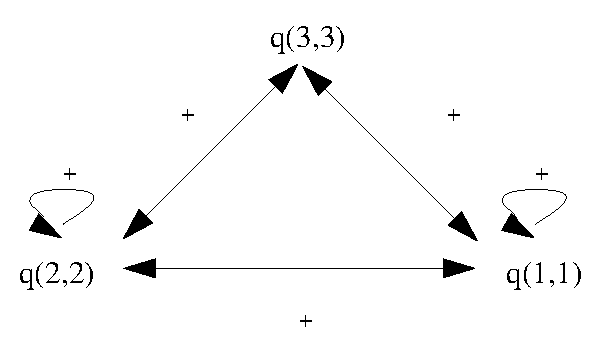
\includegraphics[width=.4\textwidth]{sdg-q-2}
%%\mbox{
%%{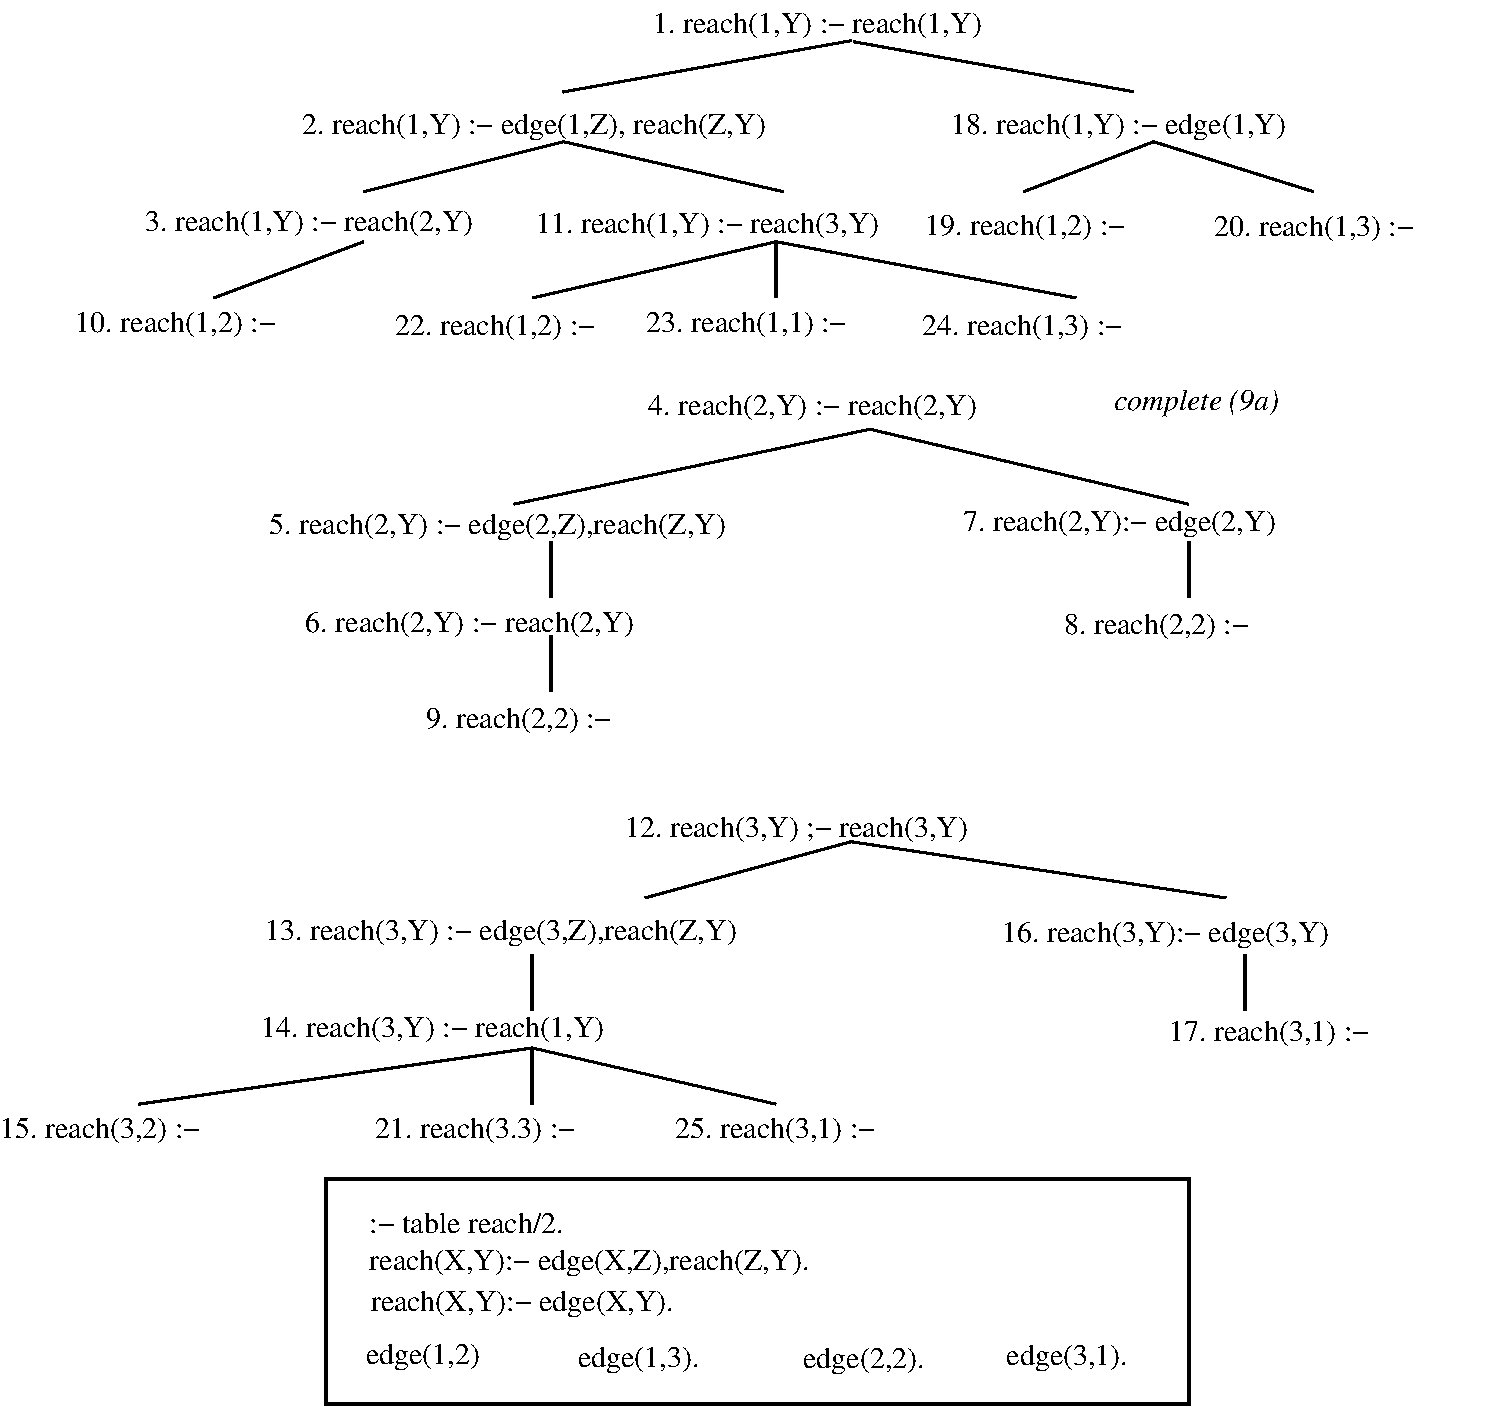
\epsfig{file=slg-forest-local,width=.99\textwidth}}}
\caption{{\em SDG for {\tt ?- q(3,3)} when the derivation is suspended by
  {\tt break/0}}c} \label{fig:sdg-break-1}
\end{figure}
%
This SDG can be produced as follows:
\begin{small}
\begin{verbatim}
| ?- q(3,3).
[ Break (level 1) ]

1: ?- get_sdg_info(F).

F = [subgoal(q(2,3),1,140253373671912,3,0,
             [140253373671672,140253373671792,140253373671912],[]),
     subgoal(q(1,3),1,140253373671792,3,0,
             [140253373671792,140253373671672,140253373671912],[]),
     subgoal(q(3,3),1,140253373671672,3,0,
             [140253373671912,140253373671792],[])]
\end{verbatim}
\end{small}

\end{example}

\ourmoditem{get\_sdg\_subgoal\_info(-SDG)}{get\_sdg\_subgoal\_info/1}{tables}
%
Note that the size of the SDG, which includes dependency edges, may be
quadratic in the number of incomplete subgoals.  When only summary
information about the subgoals in the subgoal dependency graph {\tt
  get\_sdg\_subgoal\_info/1} can be used, rather than {\tt
  get\_sdg\_info/1}.  As with the previous predicate, a list of terms of the form, 
%

{\small
\noindent
{\tt subgoal(Vertex,SCCKey,\_SubgoalKey,CallsTo,Answers,\_PosEdges,\_NegEdges)} }
%

\noindent
is returned, but {\tt \_SubgoalKey} is set to the atom {\tt null}, and
{\tt \_PosEdges} and {\tt \_NegEdges} are both set to the empty list.

This predicate has no error conditions.

\end{description}

\subsubsection{Predicates to Access the Incremental Dependency Graph} \label{sec:idg-preds}

The Incremental Dependency Graph (IDG) is used by XSB's incremental
tabling subsystem to ensure that tables that depend on dynamic facts
or rules are properly updated when the underlying dynamic code
changes.

The Incremental Dependency Graph (IDG) has as vertices those subgoals
whose predicate symbols are incrementally tabled, along with calls to
dynamic predicates that are declared as incremental.  A {\em depends}
edge exists from $S_1$ to $S_2$ iff a call is made to $S_2$ while
computing answers for $S_1$, and if there are no intervening tabled
subgoals between $S_1$ and $S_2$.  An {\em affects} edge is the
inverse of a depends edge.  Edges in the IDG are unsigned.  XSB
maintains both completed and incomplete subgoals in the IDG. (As long
as the tables for these subgoals are not abolished.)

The main predicates for inspecting the IDG as a dependency graph are,
described below.  Additionally, Section~\ref{sec:incr-preds1} contains
predicates for examining dependencies among individual subgoals, as
well as returning information about whether a subgoal in the IDG needs
to be updated or not.

\begin{description}
\ourrepeatmoditem{get\_idg\_info(+SubgoalList,-SDG)}{get\_idg\_info/2}{tables}
\ourmoditem{get\_idg\_info(-SDG)}{get\_idg\_info/1}{tables}
%

%{\bf {\em Warning: this predicate is not yet implemented}}

Returns information about the {\em Incremental Dependency Graph} (IDG)
as an adjacency list whose form is described in Section~\ref{sec:adjacency-lists}.
%
If there is an empty IDG in the current state, an empty list
is returned.

Recall from the previous section that if the SDG is accessed,
information is returned about all non-completed subgoals, all of which
depend on one another.  The IDG however may be both very large and
disconnected.  Accordingly, {\tt get\_idg\_info/2} allows a list of
subgoals to be specified, and returns information about all of the IDG
that is connected to any subgoal in the list; note that the resulting
dependency graph may also be disconnected.  If {\tt get\_idg\_info/1}
is called, information is returned about the entire IDG.

{\bf Error Cases}
\bi
\item {\tt SubgoalList} is a variable
\bi
\item 	{\tt instantiation\_error}
\ei
\item {\tt SubgoalList} is not a list
\bi
\item 	{\tt type\_error}
\ei
\item {\tt SubgoalList} contains a predicate that is not tabled
\bi
\item 	{\tt permission\_error}
\ei
\ei
\end{description}

\subsubsection{Predicates to Access the Residual Dependency Graph} \label{sec:rdg-preds}

As discussed in Section~\ref{sec:non-strat}, answers that are
undefined in the well-founded semantics are stored in XSB along with
their delay lists, forming a residual program.  The residual program
can also be represented as a Residual Dependency Graph (RDG).  Using
the RDG, a user may be able to determine why an answer $A$ to a
subgoal $S$ was unexpectedly undefined either because that answer was
involved in or depended on a loop through negation; or because the
answer depended on some other answer that was undefined because of the
use of bounded rationality (Section~\ref{sec:tabling-termination}) or
because of floundering and the use of {\tt u\_not/1}.

The representation of the RDG is slightly different from that of the
other dependency graphs.  The following example illustrates the
reasons for this.

\begin{example}\label{ex:rdg} \rm 
Consider the program 
% 
{\tt 
\begin{tabbing}
fooo\=fooooooooooooooooooooooooooooooo\=ooooooooooooo\=\kill
 \>  :- table p/2. \\
\>           p(1,2). \\
\>           p(1,3):- tnot(p(2,3)).  \\
\>           p(2,3):- tnot(p(1,3)). \> p(2,3):- r(a).\\
\>           r(a):- tnot(r(b)) \\
\>           r(b):- tnot(r(a)).   
\end{tabbing}
}
%
to which the query {?- p(1,X)} was made, generating the tables:
\begin{center}
\begin{tabular}{||l|l||}   \hline
     {\em Subgoal}                 & {\em Answers} \\ \hline \hline
     p(1,X)                     & p(1,2) \\ 
                                & p(1,3):- tnot(p(2,3))| \\ \hline
     p(1,3)                     & p(1,3):- tnot(p(2,3))| \\ \hline
     p(2,3)                     & p(2,3):- tnot(p(1,3))| \\ \hline
                                & p(2,3):- tnot(r(a))| \\ \hline
     r(a)                       & r(a):- tnot(r(b))| \\ \hline
     r(b)                       & r(b):- tnot(r(a))| \\ \hline
\end{tabular}
\end{center}

The residual dependency graph for this program and query would have a
node for each subgoal/answer combination with an undefined truth
value, and a dependency edge for nodes $S_1/A_1$ and $S_2/A_2$ if
$A_2$ occurs in a literal in the delay list for $S_1/A_1$, and the
original subgoal for $A_2$ was $S_2$ in the subcomputation for $S_1$.
The edge also has a sign indicating whether $A_2$ occurs positively or
negatively in the delay list for $A_1$.  In this example, the residual
dependency graph could be conceptually represented as 
%
\begin{verbatim}
     depends_on(p(1,X)/p(1,3),p(2,3)/p(2,3),-).
     depends_on(p(1,3)/p(1,3),p(2,3)/p(2,3),-).
     depends_on(p(2,3)/p(2,3),p(1,3)/p(1,3),-).
     depends_on(p(2,3)/p(2,3),r(a)/r(a),+).
     depends_on(r(a)/r(a),r(b)/r(b),-).
     depends_on(r(b)/r(b),r(a)/r(a),-).
\end{verbatim}
\end{example}

Thus, vertices of the RDG are subgoal/atom pairs, unlike in the other
dependency graphs where they are simply subgoals.  Summarizing, the
RDG which has as vertices those pairs of subgoals and answer atoms,
such that the truth value of the answer atom for that subgoal is {\em
  undefined} in the state of a suspended computation.  A {\em depends}
edge exists from $V_1$ to $v_2$ iff $V_2$ is a delay literal in a
conditional answer for $V_1$.  An {\em affects} edge is the inverse of
a depends edge.  Edges in the RDG are signed indicating positive or
negative dependence.\footnote{An alternative definition of the RDG has
  tabled subgoals as vertices, where subgoal $S_1$ depends on subgoal
  $S_2$ if some answer for $S_1$ depends on some answer for $S_2$.
  Such a representation can be obtained from {\tt
    get\_rdg\_info/[1,2]} below by applying a morphism, as described
  in Section~\ref{sec:dependency-graph-manipulation}.}
%
  A pair $(S,A)$ and its incident edges are removed from the RDG when
  the truth value of $A$ changes, and of course when $S$ is
  abolished.\footnote{The truth value of an atom for a given subgoal
    may change when a suspended state is further evaluated, so that
    depending when a computation is suspended, it is possible though
    rare that a given atom may have a definite truth value when
    associated with one subgoal, but the truth value may not have been
    propigated to another subgoal.  Note that the truth value of atoms
    may also change for completed subgoals when the {\sc answer
      completion} operation is lazily performed.}

Information about specific vertices and edges of the RDG can be
obtained through predicates such as {\tt get\_residual/2} and {\tt
  variant\_get\_residual/2}.

\begin{description}
\index{residual program}
\predref{get\_residual/2}
\predref{variant\_get\_residual/2}
\index{Incremental Dependency Graph (IDG)}
\index{residual dependency graph}
\ourrepeatmoditem{get\_rdg\_info(+PairList,-SDG)}{get\_rdg\_info/2}{tables}
\ourmoditem{get\_rdg\_info(-SDG)}{get\_rdg\_info/1}{tables}
%

{\bf {\em Warning: this predicate is not yet implemented}}

Returns information about the {\em Residual Dependency Graph} (RDG) as
an adjacency list whose form is described in Section~\ref{sec:adjacency-lists}.
%
If there is an empty RDG in the current state, an empty list
is returned.

Recall from the previous section that if the SDG is accessed,
information is returned about all completed subgoals.  The RDG however
may be both very large and disconnected.  Accordingly, {\tt
  get\_rdg\_info/2} allows a list of subgoal/atom pairs to be
specified, and returns information about all of the RDG that is
connected to any subgoal in the list; note that the resulting
dependency graph may also be disconnected.  If {\tt get\_rdg\_info/1}
is called, information is returned about the entire dependency graph.

{\bf Error Cases}
\bi
\item {\tt PairList} is a variable
\bi
\item 	{\tt instantiation\_error}
\ei
\item {\tt PairList} is not a list
\bi
\item 	{\tt type\_error}
\ei
\item {\tt PairList} contains a predicate that is not tabled
\bi
\item 	{\tt permission\_error}
\ei
\ei

\ourrepeatmoditem{get\_residual\_sccs(+Subgoal,+Answer,-SCCList)}{get\_residual\_sccs/3}{tables}
\ourmoditem{get\_residual\_sccs(+Subgoal,+Answer,-SCCList,-DepList,-SignList)}{get\_residual\_sccs/5}{tables}
%
%At times it can be useful to view the residual program as a directed
%graph, for instance in order to understand why a given answer might be
%undefined.  In a manner somewhat analogous to the incremental
%dependency graph (Section ~\ref{sec:incremental_tabling}) the {\em
%  residual dependency graph} is a directed graph whose nodes are
%subgoal/atom pairs and whose edges are labelled with: 1) a sign
%indicating whether the edge is positive or negative; and 2) the label
%{\em depends on} or {\em affects}.

\index{termination!radial restraint} 
\predref{u\_not/1}
%
{\bf {\em Warning: these predicates may be obsolescent.}}

The residual dependency graph can be constructed in a straightforward
way from {\tt variant\_get\_residual/2}.  However {\tt
  get\_residual\_sccs/[3,5]} provides an alternate view that is
higher-level and much faster.  Given a subgoal/answer pair as
input, each of these predicates constructs SCC-based information about
the residual dependency graph via structures of the form:
%
\begin{center}
{\tt ret(Subgoal,Answer,SCCKey)}.
\end{center}
%
where {\tt SCCKey} is a generated key for the SCC to which the
Subgoal/Answer pair belongs. Two subgoal/answer pairs are in the same
SCC iff they have the same {\tt SCCKey}; however no other dependency
information can be otherwise directly inferred from the
index~\footnote{The actual number used for each SCC key depends on how
  RDG happens to be traversed; as a result it is best to rely on the
  key only as a ``generated'' name for each SCC.}.

To obtain dependency information, {\tt get\_residual\_sccs/5} also
returns a list indicating the direct dependencies among the SCCs,
along with a list indicating whether each SCC contains a negative
edge.  For Example~\ref{ex:rdg}, the SCC information would have a form
such as:
\begin{verbatim}
[ ret(p(1,X),p(1,3),1), ret(p(1,3),p(1,3),2), ret(p(2,3),p(2,3),2),
  ret(r(a),r(a),3), ret(r(b),r(b),3) ]
\end{verbatim}
%
The dependency list would have a form such as:
\begin{verbatim}
[ depends(1,2), depends(2,3) ]
\end{verbatim}
while the sign list would have a form such as:
\begin{verbatim}
[ sign(1,no_neg), sign(2,neg), sign(3,neg) ]
\end{verbatim}
If it is necessary to know which subgoal(s) in {\tt SCC1} directly
depends on which subgoal(s) in {\tt SCC2}, the information can be
easily reconstructed from the output of {\tt
  get\_residual\_sccs/[4,5]} using {\tt variant\_get\_residual/2}.  A
similar approach can be used to determine the actual edges within a
given SCC.

SCC detection is implemented using Tarjan's algorithm~\cite{Tarj72} in
C working directly on XSB's data structures.  The algorithm is
$\cO(|V| + |E|)$ where $|V|$ is the number of vertices and $|E|$ the
number of edges in the dependency graph.  As a result, {\tt
  get\_residual\_sccs/3} provides an efficient means to materialize
the high-level topography of the dependency graph~\footnote{Currently,
  the materialization of dependency information between SCCs is
  implemented in a naive manner, so that {\tt get\_residual\_sccs/6}
  is $\cO(|V|^2)$.}.

%These predicates implement Tarjan's algorithm~\cite{Tarj72} in C
%working directly on XSB's data structures.  The algorithm is $\cO(|V|
%+ |E|)$ where $|V|$ is the number of vertices and $|E|$ the number of
%edges in the dependency graph.  As a result, these predicates provide
%an efficient means to materialize the dependency graph, even if SCC
%information per se is not required
  
\index{restraint!radial}
\index{termination!radial restraint}
\predref{u\_not/1}
\predref{get\_residual\_sccs/5}
\ourrepeatmoditem{explain\_u\_val(+Subgoal,+Answer,-Reason)}{explain\_u\_val/3}{tables}	
\ourmoditem{explain\_u\_val(+Subgoal,+Answer,-Sccs,-Deps,-Signs,-Reason)}{explain\_u\_val/6}{tables}	
%
The XSB predicate
%
{\tt explain\_u\_val(+Subgoal,+Answer,?Reason)}
\noindent
can be used to query why {\tt Answer} is undefined when derived in an
evaluation of {\tt Subgoal}.  {\tt Reason} may be
\begin{itemize}
\item {\tt negative\_loops(cycle)} if the derivation of {\tt Answer} involves a
  loop through though negation that includes {\tt Answer} itself.
%
\item {\tt negative\_loops(dependent)} if the derivation of {\tt
  Answer} depends on an atom that is involved in a loop through though
  negation.
%
\item {\tt unsafe\_negation} if the derivation of {\tt Answer} depends
  on a negative subgoal that is non-ground (XSB does not automatically
  perform subgoal reordering).  The action of making a non-ground
  subgoal undefined is performed by {\tt u\_not/1}.
%
\item {\tt bounded\_rationality} if the derivation of answer depends
  on bounded rationality based on radial restraint~\cite{GroS13}.
\end{itemize}
%
These reasons are not exclusive, and complex derivations may well
involve several of the above reasons.

{\tt explain\_u\_val/[3,6]} is based on the structures returned by
{\tt get\_residual\_sccs/[3,5]}.  While {\tt
  get\_residual\_sccs/[3,5]} is reasonably fast, it can take a
perceptable time to analyze large residual programs containing many
thousands of SCCs.  Accordingly, {\tt explain\_u\_val/6} can reuse
dependency structures returned by {\tt get\_residual\_sccs/[3,5]},
which can be useful for justification systems and other applications.

\begin{example} \rm
After executing the query {\tt p} to the program
%
\begin{verbatim}
:- table p/0, q/0, r/0, s/1.
p:- q,tnot p.                 p:- s(f(f(f(f(0))))).

q:- tnot r.                   r:- tnot q.

s(f(X)):- s(X).               s(0).
\end{verbatim}
%
where the bounded rationality size has been set to 3.  The query {\tt
  explain\_u\_val(p,P,Reason)} will bind {\tt Reason} to {\tt
  negative\_loops(cycle)}, to {\tt negative\_loops(dependent)}, and
to {\tt bounded\_rationality} (this ordering is not guaranteed).
\end{example}
\end{description}

\subsubsection{Filtering, Manipulating, and Summarizing Dependency Graphs} \label{sec:dependency-graph-manipulation}

\begin{description}
\ourmoditem{morph\_dep\_graph(+DG\_In,+Morph,-DG\_Out)}{morph\_dep\_graph/3}{tables}
%
This predicate takes as input {\tt DG\_In}, a dependency graph in
adjacency list format and returns its image, {\tt DG\_Out}, under the
graph homomorphism {\tt Morph}.  {\tt Morph} is a predicate symbol
that identifies a 2-ary predicate, {\tt Morph(+In,-Out)} that is
functional on {\tt In} and that maps the Herbrand Base of the current
program into itself.  The syntax of {\tt DG\_In} and {\tt DG\_Out} is
described at the beginning of Section~\ref{sec:adjacency-lists}.

To recall the definition of a graph homomorphism (cf. e.g.,
~\cite{Hara69}) a functional notation is used for {\tt Morph/2}.  {\tt
  DG\_Out} is a graph such that the vertices of {\tt DG\_Out},
$vertices({\tt DG\_Out})$ is the set:
\[
\{ morph(V) | V \in vertices({\tt DG\_In}) \}
\]
while the edges of {\tt DG\_Out}, $edges({\tt DG\_Out})$ are the sets
\[
\{ \langle morph(V_1),morph(V_2) \rangle | \langle V_1,V_2 \rangle \in edges({\tt DG\_In}) \}
\]
We adapt this definition to signed dependency graphs by mapping all
positive adjacent edges into a positive set, and negative adjacent
edges into a negative set.

The power of {\tt morph\_dep\_graph/3} arises when the numbers of
vertices and edges of {\tt DG\_In} is large, and {\tt morph/2} ensures
that numbers for {\tt DG\_Out} are much smaller -- thus allowing
recognizable patterns to emerge.

For efficiency reasons, a special condition, ${\cal C}_1$, is assumed
  about {\tt morph/2}: that if two elements of its range unify, then
  they must be identical.  For instance, a morphism $M_1$ that reduced
  the maximum depth of each non-variable argument of a term by 1 would
  not fit this condition, since $M_1(f(a,g(h(b)))) = f(X_1,g(h(X_2)))$
  while $M_1(f(a,g(b))) = f(X_1,g(X_2))$, which unify.  On the other
  hand, a morphism that abstracts each argument to have a maximal
  fixed depth would fulfill the condition.  In any case, as long as
  ${\cal C}_1$ is observed, {\tt morph/2} may instantiated by an
  abstraction function as used elsewhere in this manual: i.e., a
  function such that $morph(Term)$ subsumes $Term$.  However, other
  morphisms may also be useful as demonstrated in
  Example~\ref{ex:morph-sdg} below.

While the syntax of {\tt SDG\_Out} is the same as that of {\tt SDG\_In},
the meaning of the arguments differs slightly.  {\tt SDG\_Out} is a
list of terms of the form:

{\tt subgoal(MorphSubg,null,Key,CallsTo,Answers,PosKeyList,NegKeyList)} 

such that 

\bi
\item {\tt MorphVert} is $morph({\tt Vertex})$ for one or more
  subgoals that are vertices of {\tt DG\_In}
\item The second argument, which represents SCC information in the
  original dependency graph, is the atom {\tt null} when a morphism is
  applied, since SCC information is not preserved in general.
\item {\tt Key} is an atom identifying {\tt MorphVert}.  Note that
  while each subgoal in {\tt DG\_In} corresponds to e.g., a tabled
  subgoal, a given subgoal image in {\tt DG\_Out} may not correspond to
  a tabled subgoal in the current state.  Thus a table entry handle
  may not be available, so generated keys are used in {\tt DG\_Out}.
\item {\tt CallsTo} If {\tt DG\_In} originated from an SDG or IDG, {\tt
  CallsTo} is the sum of the number of calls to every subgoal $S \in$
  {\tt DG\_In} such that $morph(S) = {\tt MorphVert}$.  Otherwise, {\tt
    CallsTo} is 0.
\item {\tt Answers} If {\tt DG\_In} originated from an SDG or IDG, {\tt
  Answers} is the sum of the number of answers for every subgoal $S
  \in$ {\tt DG\_In} such that $morph(S) = {\tt MorphVert}$.  Otherwise,
     {\tt Answers} is 0.
\item {\tt PosKeyList} is a list of the keys to those vertices adjacent
  to {\tt MorphSubg} with positive sign as described above.
\item {\tt NegKeyList} is a list of the keys to those vertices adjacent
  to {\tt MorphSubg} with negative sign as described above.
\ei

\begin{example} \rm \label{ex:morph-sdg}
Continuing Example~\ref{ex:get-sdg}, let {\tt mymorph} identify the
predicate

\begin{verbatim}
mymorph(Term,NewTerm):-
        Term =.. [F,A1,A2],
        map_arg_1(A1,NewA1),
        NewTerm =.. [F,NewA1,A2].

map_arg_1(2,1):- !.
map_arg_1(X,X).
\end{verbatim}
Thus {\tt mymorph/2} maps {\tt q(2,1)} to {\tt q(1,1)} and maps
both {\tt q(1,1)} and {\tt q(3,1)} to themselves.  Then if {\tt DG\_In}
is instantiated to the SDG produced in Example~\ref{ex:get-sdg}, the
goal {\tt ?- morph\_dep\_graph(DG\_In,mymorph,DG\_Out)} would produce:

\begin{verbatim}
SDG\_Out = [subgoal(morph80,q(1,3),6,0,[morph80,morph81],[]),
          subgoal(morph81,q(3,3),3,0,[morph80],[])
\end{verbatim}
\end{example}

{\bf Error Cases} 
\bi
\item 	{\tt Morph} is not an atom
\bi
\item 	{\tt type\_error}
\ei
%
\item 	{\tt DG\_Out} is not a variable
\bi
\item 	{\tt type\_error}
\ei
%
\item 	{\tt DG\_In} is not an adjacency list as described above
\bi
\item 	{\tt misc\_error}
\ei
\ei
%
\ourmoditem{dep\_graph\_scc\_info(+SDG,-ListOut)}{dep\_graph\_scc\_info/2}{tables}
%
Given an SDG representation in the adjacency list format described
above, this predicate returns information about the SCCs that are
currently under evaluation.  Upon success {\tt ListOut} will contain a
term

{\tt scc(SCCIndex,NumSubgoals,NumAnswers,NumPosEdges,NumNegEdges)}

for each SCC under evaluation, such that:

\bi
\item {\tt SCCIndex} is the index of the SCC
\item {\tt NumSubgoals} is the number of subgoals in the SCC
\item {\tt NumAnswers} is the total number of answers for all subgoals in the SCC
\item {\tt NumPosEdges} is the total number of positive edges within the SCC.
\item {\tt NumNegEdges} is the total number of negative edges within the SCC.
  \ei

\ourmoditem{print\_sdg\_info}{print\_sdg\_info/0}{tables}
%
Prints the current SDG to {\tt stdout} in a readable
manner.\footnote{This predicate, along with {\tt
    print\_sdg\_subgoal\_info/0} replaces the predicate {\tt
    print\_incomplete\_tables/0}, which was included in previous
  releases.}

\ourmoditem{print\_sdg\_subgoal\_info}{print\_sdg\_subgoal\_info/0}{tables}
%
Prints summary subgoal information about the current SDG to {\tt stdout} in a
readable manner.

\ourmoditem{print\_dep\_graph(+DG)}{print\_dep\_graph/1}{tables}
%
Prints a dependency graph {\tt DG} (whether its an SDG, IDG, or RDG)
to {\tt stdout} in a simple, but readable manner.
%
\begin{example}
Continuing from Example~\ref{ex:morph-sdg}, if 

\begin{verbatim}
SDG = [subgoal(morph80,q(1,3),6,0,[morph80,morph81],[]),
          subgoal(morph81,q(3,3),3,0,[morph80],[])
\end{verbatim}

then {\tt print\_dep\_graph(SDG)} would output

\begin{verbatim}
Subgoal: q(1,3)
        Number of calls to this subgoal 6; Number of answers 0
        Affects positively q(1,3) ; q(3,3)
Subgoal: q(3,3)
        Number of calls to this subgoal 3; Number of answers 0
        Affects positively q(1,3) 
\end{verbatim}
\end{example}

\end{description}

\subsection{Summary: Inspection Predicates}

XSB provides a number of ways to inspect a tabled derivation,
including directly through the tables, or through one of the
dependency graphs: the IDG, RDG or SDG.  Specifically, some useful
inspection predicates available in XSB are:

\begin{itemize} 
\item {\tt statistics/[0,1,2]} (Section~\ref{environmental}) is a
  highly useful general-purpose predicate that provides an important
  summary of how memory is used by the XSB process or thread, the
  amount of time used by the process or thread, along with various
  counts of tabling operations and measures of table space.

\item {\tt table\_dump/[2,3]} (Section~\ref{sec:table-dump}) allows
  directed and iterative inspection of the current set of tabled
  subgoals and their answers, at various levels of summary
  aggregation.

\index{Incremental Dependency Graph (IDG)} 
\index{residual program}
\index{residual dependency graph}
\item Inspection of the Incremental Dependency Graph can be made via
  the predicate {\tt get\_idg\_info/[1,2]}
\footnote{These predicates
    are not yet implemented: although {\tt tt get\_incr\_sccs/[1,2]},
    and {\tt get\_incr\_sccs\_with\_deps/[2,3]} have been.} together
  with predicates for dependency graph manipulation such as {\tt
    morph\_dep\_graph/3} and {\tt dep\_graph\_scc\_info/3}
  (cf. Section~\ref{sec:dependency-graph-manipulation}).
%
 More targeted inspection of specific edges and dependencies of the
 Incremental Dependency Graph is supported through {\tt
   incr\_directly\_depends/2} and {\tt incr\_trans\_depends/2}
 (cf. Section~\ref{sec:incr-preds1}).

\item Inspection of the Subgoal Dependency Graph can be obtained
  through the predicate {\tt get\_sdg\_info/1}, and its information
  analyzed through predicates for dependency graph manipulation such
  as {\tt morph\_dep\_graph/3}, and {\tt dep\_graph\_scc\_info/2}
  (cf. Section~\ref{sec:dependency-graph-manipulation}).  Note that
  {\tt get\_sdg\_info/1} returns information concerning incomplete 
  subgoals {\em only}.

\item Inspection of the Residual Dependency Graph can be made via the
  predicate {\tt get\_rdg\_info/[1,2]},\footnote{This predicate is not
    yet implemented: although {\tt tt get\_residual\_sccs/[1,2]} has
    been.} together with dependency graph manipulation predicates such
  as {\tt morph\_dep\_graph/3} and {\tt dep\_graph\_scc\_info/3}.
  (cf. Section~\ref{sec:dependency-graph-manipulation}).  The
  predicates {\tt get\_residual/2} and {\tt variant\_get\_residual/2}
  allow the residual program to be viewed as sets of clauses.
  Finally, {\tt explain\_u\_val/3} can be used to indicate why a given
  atom has the truth value {\em undefined} rather than {\em true} or
  {\em false} (cf. Section~\ref{sec:table-inspection}).
\end{itemize}

All of these predicates, except for {\tt get\_sdg\_info/1}, can be
used to retrospectively analyze any completed derivation, as long as
the derivations tables have not been abolished.  In addition, all of
the predicates can be used to analyze an ongoing derivation by
suspending the derivation and then examining the computation from a
subsidiary command-line interpreter.  This can be especially important
for long-running computations or those that take a lot of space.

In XSB, a computation can be suspended in several ways, depending a
user's tastes in and needs for debugging:

\bi 
\item By a call to {\tt break/0}.  This is usually best done by
  calling {\tt break/0} as part of a handler for {\tt timed\_call/2},
  but {\tt break/0} can also be called explicitly from a program.
%
\item By hitting ctrl-C if XSB is running in stand-alone mode

\item By setting a {\em tripwire} as introduced below
  (Section~\ref{sec:tripwire}).  
%
\ei

\index{tripwires}
\subsection{Setting Tripwires on Tabled Derivations} \label{sec:tripwire}
%
A tripwire represents an unexpected property of a derivation: such as
an excessive use of time or memory; an unexpected number or complexity
of tabled subgoals or answers; or an unexpected number of mutually
dependent tabled subgoals.  Depending both on the class of a tripwire
and on how XSB's flags are set, a tripwire may have different effects.
Any tripwire may be treated as an error so that it throws an exception
just as any other error.  {\em Inspectable} tripwires may additionally
be considered as inspection points, and when hit may suspend the
derivation and create a break point.\footnote{Note that such a
  suspension makes available for inspection the state of the
  derivation at the point the tripwire was activated.  If inspection
  points were implemented using ISO errors, state could only be made
  available at the point where the error was {\em caught}, whose state
  may differ greatly from the point where the error occurred (i.e.,
  where the tripwire was hit).}
%
In such a case, a short explanation will be made of how a tripwire was
encountered, along with suggestions about how to further inspect the
suspended derivation.\footnote{
  %% 
  This is the default behavior for XSB:
  handling of tripwires can be overridden by the user,
  as explained later in this section.
}
%%
{\em Correctable} tripwires are a subset of
inspectable tripwires for which an automatic action may be taken to
remedy the situation, such as rewriting a subgoal or an answer whose
size is greater than a given limit, by using subgoal abstraction, 
answer restraint or sound completion of a subgoal.

Tripwires may be set in various ways: most can be set and viewed at a
session level using Prolog flags, others can also be set at the
predicate level via the {\tt table/1} declaration, while still others
can only be set by explicit programming.  Tripwires thus represent a
coordinated set of tools for understanding bounds on a tabled
derivation, rather than a unified API.

For a tripwire {\tt T} that can be set and viewed as a Prolog flag,
the flag name has the form {\tt tripwire(T)}, and this flag has two or
more values.  An {\em action}, designated {\tt action(A)}, indicating
the action to take such as {\tt error}, {\tt suspend}, or other
actions; and one or more parameters, designated {\tt limit(P)}.
For example, if a user wants to be able to suspend and inspect a
computation whenever it has an active recursive component (SCC) with
over 100 subgoals, she can execute the following directives:

{\tt ?- set\_prolog\_flag(tripwire(max\_scc\_subgoals),limit(100)).}

{\tt ?- set\_prolog\_flag(tripwire(max\_scc\_subgoals),action(suspend)).}

We discuss various types of tripwires in turn, and provide informal
guidelines for inspecting a derivation when a given tripwire has been
hit.

\subsubsection{Tripwires Based on Resource Limits}
%
Hitting a resource tripwire reflects the fact that a derivation is
taking more time or using more memory than expected.  A resource
tripwire is a user-imposed limit, rather than an external limit
imposed by the platform or operating system, and thus differs from an
ISO resource error.

\index{tripwires!timed call} 
\predref{timed\_call/2}
\predref{timed\_call\_modify/1}
%
Time-based resource tripwires can easily
be programmed using a handler to {\tt timed\_call/2}.  Time-based
tripwires are inspectable, so such a handler might throw an error
after a derivation has taken a certain amount of CPU time, or call
{\tt break/0} to implement periodic inspection points, or implement
other periodic analytics or monitoring.  The parameters for timed call
can be changed whenever the timed call is suspended by {\tt
  timed\_call\_modify/1}.  See Section~\ref{sec:timed-call} for more
details.

\index{tripwires!max\_memory} An inspectable memory-based resource
tripwire can be set via the Prolog flag {\tt tripwire(max\_memory)},
so that the tripwire will be hit whenever XSB uses more than a given
total amount of memory.  This amount can be set either as an integer,
representing an absolute number of kilobytes or as a floating point
number indicating a percentage of the RAM of the platform upon which
XSB is executing.  
%Currently, a memory-based tripwire can only throw an error.

\paragraph{Guidelines for Analysis of Resource-based Tripwires}  \ \\

{\bf {\em Note that the numbers and sizes below are for example
    purposes only.  If memory limits are set to, say, a gigabyte or
    more of memory, and time limits are set to several seconds, the
    numbers and sizes may be several orders of magnitude more than
    those shown below.}}

If a resource tripwire is hit, the best course of analysis usually
starts with viewing the output of {\tt statistics/[0,1]}.  
\bi
\item {\em Check whether there are a large number of incomplete
  tables} This can be determined, for instance, using the output of
  {\tt statistics/0}, by a line near the end of the memory
  table.~\footnote{This line is not printed out if there are no
    incomplete tables.}  E.g.:
%
{\small \begin{verbatim}
        (501227 incomplete table(s) in 89 SCCs)
\end{verbatim} }

\bi
\item If there are a large number of incomplete tables, XSB's stack
 space is likely to be high also, since an incomplete table $T$ needs
 to maintain many details of its derivation state to ensure all
 answers for $T$ are returned to all calls to $T$.  In this case, the
 predicates can be used that analyze the Subgoal Dependency Graph of
 the suspended derivation (Section~\ref{sec:sdg-preds}).  {\em Note
 that, here and below, when there are a large number of incomplete
 tables, information returned by {\tt get\_sdg\_info/1}, as well as by
 {\tt get\_idg\_info/1} and {\tt get\_rdg\_info/1} may need to be
 filtered or manipulated using the predicates in
 Section~\ref{sec:dependency-graph-manipulation}.}  \ei

\item {\em Otherwise, check whether there are a large number of
 completed subgoals.} If there are not many incomplete tables but the
 table space seems large, {\tt statistics/[0,1,2]} indicates both the
 total number of tabled subgoals and the total number of answers,
 either of which may be the culprit.  For instance, the beginning of
 the summary of tabling operations might contain information such as:

%
{\small 
\begin{verbatim}
 Tabling Operations
  12 subsumptive call check/insert ops: 9 producers, 3 variants,
  0 properly subsumed (0 table entries), 0 used completed table.
  0 relevant answer ident ops.  0 consumptions via answer list.
  1065417 variant call check/insert ops: 938125 producers, 127292 variants.
  46210 answer check/insert ops: 46210 unique inserts, 0 redundant.
\end{verbatim} } 

This indicates that there are 1,065,417 subgoals (complete or
 incomplete) tabled with call variance, and 12 subgoals tabled with
 call subsumption.  Among all subgoals there are 46,210 answers.  
%
\bi
\item To understand details of overall table space usage, {\tt
  table\_dump/[2,3]} can be called to provide further information
  (Section~\ref{sec:table-dump}).  
\ei
%
\item {\em Check whether the IDG is large.}  In addition to simply
  having a large number of subgoals (incomplete or complete) and
  answers, the use of incremental dependency, which maintains an IDG,
  has an effect on memory.  {\tt statistics/[0,1]} indicates when
  incremental tabling is being used heavily, by a line towards the
  bottom of the output, such as:
%Total number of incremental subgoals created: 50
{\small \begin{verbatim}
Currently 501688 incremental subgoals, 781432 dependency edges
\end{verbatim} }
%
\bi
\item When there are large numbers of incrementally tabled subgoals
  and dependency edges, {\tt get\_idg\_info/1}
  (Section~\ref{sec:idg-preds}) can be used to obtain a global view of
  the IDG.  Note that incremental tabling does require more memory for
  completed tables than non-incremental tabling, due to the need to
  retain the IDG so that tables can be updated when dynamic code
  changes.
%
\ei
\item {\em Check whether there are a large number of answers whose
  truth value is {\em undefined}}.  This is indicated, for instance,
  by lines at the end of the summary of tabling operations in {\tt
    statistics/0}.~\footnote{These lines are not printed out if there are no
    incomplete tables.}  E.g.:
{\small \begin{verbatim}
   80005 DEs in the tables (space: 3932480 bytes allocated, 3840560 in use)
   40005 DLs in the tables (space: 983200 bytes allocated, 960280 in use)
\end{verbatim} }
%
\bi
If there is indication that there are a large number of answers with
 truth value {\em undefined}{\tt get\_rdg\_info/[1]} and/or {\tt
 explain\_u\_val/2} can be used to understand the dependencies among
 these answers.  
\ei
\ei

\subsubsection{Tripwires Based on Properties of a Tabled Derivation}
%
Theoretically speaking, in a pure logic program if a tabled derivation
 is not terminating it is because there are an unbounded number of SLG
 trees, or because one or more of the SLG trees is of unbounded size.
  The former case indicates that a computation has an unbounded number
 of subgoals, while the latter indicates that one or more subgoals has
 an unbounded number of answers.  In a similar manner, terminating but
 expensive derivations also may have too many subgoals, too many
 answers, or too many dependencies among incomplete subgoals.  We
 consider these cases in turn.

\bi
\item {\em There are too many tabled subgoals} 
\bi
\item {\em There are a potentially unbounded number of tabled subgoals
 in a pure program.}\/ In this case, there must be a potentially
 unbounded number of {\em distinct} tabled subgoals in the derivation.
  If this happens using ca`v`vll variance, this situation can
 sometimes be addressed by using call subsumption instead.  However
 termination can {\em always} be ensured by using subgoal abstraction,
 as long as a derivation produces only a finite number of answers
 (cf. Section~\ref{sec:tabling-termination} and \cite{RigS14}).  XSB
 allows subgoal abstraction to be applied based on term size either
 globally through the tripwire {\tt max\_table\_subgoal\_size}, or on
 a predicate-by-predicate basis through tabling directives.  In other
 words, when a tabled subgoal, $S_{big}$, is called whose size is
 greater then the limit specified for its predicate, a tripwire is
 activated, and various actions can be specified.  In many -- perhaps
 most -- cases, the best action is simply to abstract $S_{big}$.
  However it is also possible to suspend and inspect the derivation so
 that the causes that led to $S_{big}$ can be analyzed.  As a final
 alternative, an error can be thrown, which is the default action.

\item {\em There are a potentially infinite number of subgoals in a
 program with arithmetic.}.  Due to the manner in which numbers are
 represented in XSB, XSB's size metric would permit a potentially
 infinite number of subgoals if numbers occurred within these
 subgoals.  The tripwire {\tt max\_incomplete\_subgoals} allows a
 limit to be set on the maximal number of incomplete subgoals.  If a
 derivation exceeds that limit, the computation may be suspended, or
 an error thrown.

\item {\em There are a finite but large number of tabled subgoals.}\/
 A separate problem from those above can happen as follows.  If a
 program is written over a language that has a finite but large number
 of constant symbols, then a program that generates subgoals of the
 form
\[
   p(c_i,c_j,c_k,X)
\]
  will theoretically terminate, but may be too inefficient for
 practical purposes.  This problem can be addressed by the tripwrite
 {\tt max\_incomplete\_subgoals} just discussed, but it is often
 helpful to have a different size limit for cases where there are a
 large number of subgoals within the {\em same} SCC.

 The tripwire {\tt max\_scc\_subgoals} allows such a limit to be set
 on the maximal number of incomplete subgoals in any recursive
 component.  If a derivation exceeds that limit, the computation may
 be suspended, or an error thrown.  This situation is similar to that
 of simply having too many incomplete subgoals, but may suggest a
 different focus when analyzing a suspended computation.  In addition,
 the number of dependencies can rise quadratically with the absolute
 size of an SCC.  As a result, it often makes sense to have different
 limit for the size of a single (incomplete) SCC and for the number of
 incomplete subgoals overall.
%

{\em Guidelines for Analysis} If the computation is producing too many
 tabled subgoals the suspension may have been triggered by one of the
 tripwires: {\tt max\_table\_subgoal\_size}, {\tt
 max\_incomplete\_subgoals} or {\tt max\_scc\_size}.  In any of these
 cases, the suspension or error message will indicate the tripwire
 that has been hit.  The number of incomplete subgoals can be seen
 from the output of {\tt statistics/0}.  The inspection predicates of
 Section~\ref{sec:dep-graph} can be used to examine these subgoals and
 their dependencies.
%
\ei
\ei 

\bi

\item {\em There are too many tabled answers.} The approaches to this
  situation are similar in spirit to the cases of too many subgoals.
%
\bi
\item {\em One or more subgoals has an unbounded number of answers.}
  In this case, termination can be ensured by using radial restraint,
 which abstracts answers in a manner that is sound with respect to the
 well-founded semantics and can ensure that a derivation will produce
 only a finite number of answers
 (cf. Section~\ref{sec:tabling-termination} and\cite{GroS13}), XSB
 allows radial restraint to be applied based on term size in two ways.
  First, restraint can be applied globally through the tripwire {\tt
 max\_table\_answer\_size}.  Second, XSB allows restraint to be
 declared at a predicate-by-predicate basis.  In other words, when an
 answer, $A_{big}$, is to be added to a table, and its size is greater
 then the limit specified for its predicate, a tripwire is activated,
 and various actions can be specified.  In many cases, the best action
 is simply to abstract $A_{big}$, which gives it the truth value {\em
 undefined} for that answer. However it is also possible for the
 derivation to be suspended so that the causes that led to $A_{big}$
 can be analyzed.  As a final alternative an error can be thrown; this
 is the default action for XSB.

\item {\em There are a finite but large number of tabled answers.}\ As
  with subgoals, checking for the depth of an answer may not catch
  certain causes of inefficiency. If a program is written over a
  language that has a large number of constant symbols, then a program
  that generates answers of the form
\[
   p(c_i,c_j,c_k,c_l)
\]
  will theoretically terminate, but may be too inefficient for
  practical purposes.  

 To address such situations, XSB has the tripwire {\tt
 max\_answers\_for\_subgoal} which is hit if any subgoal has more than
 the specified number of answers.  If a derivation exceeds that limit,
 the subgoal may be eagerly completed while maintaining soundness, the
 the computation may be suspended, or an error thrown
 (cf. Section~\ref{sec:answer-count-restraint} for a discussion of how
 a subgoal may be completed early while preserving soundness).
%
 \ei {\em Guidelines for Analysis} If the computation is producing too
 many tabled answers, a suspension may be triggered by one of the
 tripwires: {\tt max\_table\_answer\_size}, or {\tt
 max\_answers\_for\_subgoal}.  In any of these cases, the suspension
 (or error message) will indicate the subgoal whose number of answers
 hit the tripwire.  The number and shape of answers for that subgoal
 and others can be viewed through the {\tt table\_dump} library
 (Section~\ref{sec:table-dump}).  If some answers are undefined, the
 predicates {\tt get\_rdg\_info/1} and {\tt explain\_u\_val/2} can be
 used to explore dependencies among the answers.  In addition,
 dependency graph analysis based on the predicates {\tt
 get\_sdg\_info/1} and {\tt get\_idg\_info/1} can help locate areas of
 code that caused the profusion of answers.

 \ei

\subsubsection{The Suspend Action for Flag-Based Tripwires}

If the action {\tt suspend} is specified for a given flag-based
 tripwire $T$, (i.e., a tripwire other than one based on {\tt
 timed\_call/2}), then hitting $T$ causes XSB to take a given action.
  By default, this action is to enter a break level from which the
 computation can be inspected. (This default action for {\tt suspend}
 can be overridden.)  A preamble to the break level is also presented
 that describes certain values pertaining to the state of the
 computation, along with an attempt to summarize what the situation
 means.  The preamble for the tripwire {\tt max\_incomplete\_subgoals}
 appears as follows.

%----------------------------------------------------------------------------------------
\begin{small}
\begin{verbatim}
There are currently 11 incomplete tabled subgoals, which exceeds the limit set by the 
flag 'max_incomplete_subgoals'.  These subgoals are in 11 separate recursive components.

The number of incomplete recursive components is close to the number of incomplete 
subgoals, and furthermore, nearly all of these recursive components are trivial.

This information indicates a likelihood that the program is performing some sort of 
structural recursion using tabling (i.e., recursing through a list, performing numeric 
iteration, etc.)

To remedy, check that the recursion is well-founded.  If so, consider executing the 
recursion using a non-tabled predicate, or consider using hash-cons tabling to reduce 
the space required for tables, then increase the value of the flag.

  * To continue, reset the flag and then type Ctrl-d
  * To abort the suspended derivation, enter the command 'abort/0'
  * To inspect the incomplete tabled subgoals, enter the command 'print_sdg_info/0'
\end{verbatim}
\end{small}
%----------------------------------------------------------------------------------------

From within a break level thrown by a tripwire, a user can perform
 most queries and commands with two important exceptions.

\begin{itemize}
\item No tabled goals or subgoals may be executed.  Of course once the
 break is exited, the original computation can be continued, and
 tabled subgoals can be executed as usual.
\item Reconsulting a file containing code upon which the original
 query depends may throw an error.
\end{itemize}

There are situations where the action of breaking to allow a user can
 inspect a query isn't suitable -- if XSB is embedded into a process,
 for instance, or is part of some other application.  In such a case,
 the user can override XSB's default behavior by asserting into the
 {\tt user} module a {\em tripwire handler}, which will be executed
 when a given tripwire is hit.  For instance, the tripwire {\tt
 max\_table\_subgoal\_size} would use the tripwire {\tt
 max\_table\_subgoal\_size\_user\_handler/0}.  Subject to the
 constraints above, the handler may perform any actions desired,
 including increasing the tripwire limit, adjusting its action,
 changing runtime tabling properties, or simply writing to a
 log.\footnote{As a further example, when XSB supports the language
 Ergo the tripwire may set on forest logging to support termination
 analysis via the Terminyzer tool.}

A handler that is called when a tripwire is hit has some resemblances
 to a handler called when an error is caught, but there are important
 differences.  A condition triggering a tripwire might or might not
 reflect an error in a program.  So the handler is invoked when the
 tripwire is hit, rather than after exiting portions of that
 derivation as is the case when an error is caught.  If the user wants
 to exit some or all of a derivation when a tripwire is hit, it is
 simple to change the tripwire's action to error, and arrange to catch
 the error with a suitable handler.

\subsubsection{Summary of Flag-Based Tripwires}
%
Each of the tripwires described below can be queried and set via
 prolog flags.  For instance the query

\begin{verbatim}
| ?- current_prolog_flag(tripwire(max_table_subgoal_size),Property).

Property = limit(12)
Property = action(error);
\end{verbatim}
indicates the current values of this tripwire.  (Also see the
 description of Prolog flags in Section~\ref{State}.)

%\paragraph*{Tripwire Description
\begin{itemize}

\index{tripwires!max\_table\_subgoal\_size} 
\item {\tt max\_table\_subgoal\_size}. 
\bi  
\item {\em Limit:} The maximum size of a given argument in a subgoal
 (cf. Section~\ref{sec:size-metric}).  A limit of {\tt 0} means that
 this tripwire is disabled.
\item{\em Possible actions:} {\tt abstract}, {\tt suspend}, {\tt error}
 or {\tt custom}
\item {\em Default.} Limit: {\tt 0}; Action: {\tt error}.
\item {\em User handler for custom}: {\tt
 max\_table\_subgoal\_size\_handler}.  
\ei

\index{tripwires!max\_incomplete\_subgoals} 
\item {\tt max\_incomplete\_subgoals}
\bi  
\item {\em Limit:} The maximum number of subgoals that are
 incomplete at any given time.  A limit of {\tt 0} means that
 this tripwire is disabled.
\item{\em  Possible actions:} {\tt suspend}, {\tt error}, or {\tt custom}.
\item {\em Default.} Limit: {\tt 0}; Action: {\tt error}.
\item {\em User handler for custom}: {\tt max\_incomplete\_subgoals\_user\_handler}.
\ei

\index{tripwires!max\_scc\_subgoals} 
\item {\tt max\_scc\_subgoals}
\bi  
\item {\em Limit:} The maximum number of subgoals that are incomplete,
 and are in the same SCC at any given time.  A limit of {\tt 0} means
 that this tripwire is disabled.
\item{\em  Possible actions:} {\tt suspend}, {\tt error} or {\tt custom}.
\item {\em Default.} Limit: {\tt 0}; Action: {\tt error}.
\item {\em User handler for custom}: {\tt max\_scc\_subgoals\_user\_handler}.
\ei

\index{tripwires!max\_table\_answer\_size} 
\item {\tt max\_table\_answer\_size}
\bi  
\item {\em Limit:} The maximum size of a given argument of an answer
 (cf. Section~\ref{sec:size-metric}).  A limit of {\tt 0} means that
 this tripwire is disabled.
\item{\em Possible actions:} {\tt abstract}, {\tt suspend}, {\tt
 error} or {\tt custom}
\item {\em Default.} Limit: {\tt 0}; Action: {\tt error}.
\item {\em User handler for custom}: {\tt max\_table\_answer\_size\_user\_handler}.
\ei

\index{tripwires!max\_answers\_for\_subgoal} 
\item {\tt max\_answers\_for\_subgoal}
\bi  
\item {\em Limit:} The maximum number of answers for any single tabled
 subgoal.  A limit of {\tt 0} means that
 this tripwire is disabled.
\item{\em Possible actions:} {\tt complete\_soundly}, {\tt suspend},
 {\tt error} or {\tt custom}.
\item {\em Default.} Limit: {\tt 0}; Action: {\tt error}.
\item {\em User handler for custom}: {\tt max\_answers\_for\_subgoal\_user\_handler}.
\ei

\item {\tt max\_memory}
\bi  
\item {\em Limit:} If an integer, the limit is the maximum
 amount of memory allowed for a computation, in kilobytes.  If a
 floating-point number, the limit is the proportion of RAM for the
 machine on which XSB is running.  A limit of {\tt 0} means that
 this tripwire is disabled.
\item{\em Possible actions:} {\tt suspend}, {\tt error} or {\tt custom}.
\item {\em Default.} Limit: {\tt 0}; Action: {\tt error}.
\item {\em User handler for suspend}: {\tt max\_memory\_user\_handler}.
\ei

\end{itemize}

%%% Local Variables: 
%%% mode: latex
%%% TeX-master: "manual1"
%%% End: 


\chapter{Definite Clause Grammars} \label{DCGs}
\index{definite clause grammars}\index{grammars!definite clause}
%===============================================================

\section{General Description}
%============================

Definite clause grammars (DCGs) are an extension of context free
grammars that have proven useful for describing natural and formal
languages, and that may be conveniently expressed and executed in
Prolog.  A Definite Clause Grammar rule is executable because it is
just a notational variant of a logic rule that has the following
general form:
\begin{center}
                {\em Head} {\tt \verb|-->|} {\em Body.}
\end{center}
with the declarative interpretation that ``a possible form for {\em
Head} is {\em Body}''. The procedural interpretation of a grammar rule
is that it takes an input sequence of symbols or character codes,
analyses some initial portion of that list, and produces the remaining
portion (possibly enlarged) as output for further analysis.  In XSB,
the exact form of this sequence is determined by whether XSB's {\em
DCG mode} is set to use tabling or not, as will be discussed below.
In either case, the arguments required for the input and output lists
are not written explicitly in the DCG rule, but are added when the
rule is translated (expanded) into an ordinary normal rule during
parsing.  Extra conditions, in the form of explicit Prolog literals or
control constructs such as {\em if-then-elses} ({\tt '->'/2}) or {\em
cuts}\index{cut} (\cut)\predrefindex{"!/0}, may be included in the {\em
Body} of the DCG rule and they work exactly as one would expect.

The syntax of DCGs is orthogonal to whether tabling is used for DCGs
or not.  An overview of DCG syntax
 supported by XSB is as follows:
\begin{enumerate}
\item A non-terminal symbol may be any HiLog term other than a variable
      or a number. A variable which appears in the body of a rule is
      equivalent to the appearance of a call to the standard predicate
      {\tt phrase/3} as it is described below.
\item A terminal symbol may be any HiLog term. In order to distinguish 
      terminals from nonterminals, a sequence of one or more terminal
      symbols   $\alpha, \beta, \gamma, \delta, \ldots$
      is written within a grammar rule as a Prolog list 
         {\tt [} $\alpha, \beta, \gamma, \delta, \ldots$ {\tt ]},
      with the empty sequence written as the empty list {\tt [\,]}.
      The list of terminals may contain variables but it has to be a 
      proper list, or else an error message is sent to the standard 
      error stream and the expansion of the grammar rule that contains 
      this list will fail. If the terminal symbols are UTF-8 character
      codes, they can be written (as elsewhere) as strings.
\item Extra conditions, expressed in the form of Prolog predicate calls, 
      can be included in the body (right-hand side) of a grammar rule by 
      enclosing such conditions in curly brackets, {\tt '$\{$'} and
      {\tt '$\}$'}.
      For example, one can write:
      \begin{center}
                {\tt positive\_integer(N) \verb|-->| [N], $\{$integer(N), N > 0$\}$.}
                \footnote{A term like {\tt $\{$foo$\}$} is just a
			  syntactic-sugar for the term {\tt '$\{\}$'(foo)}.}
      \end{center}
\item The left hand side of a DCG rule must consist of a single non-terminal,
      possibly followed by a sequence of terminals (which must be written as
      a {\em unique} Prolog list). Thus in XSB, unlike SB-Prolog 
      version 3.1, Semicontext (formerly called push-back lists) is supported.
\item The right hand side of a DCG rule may contain alternatives (written 
      using the usual Prolog's disjunction operator {\tt ';'} or 
      using the usual BNF disjunction operator {\tt '|'}. 
\item The Prolog control primitives {\em if-then-else} ({\tt '->'/2}),
      {\em nots} ({\tt not/1, fail\_if/1}, \not\ or {\tt tnot/1}) and 
      {\em cut}\index{cut} (\cut)\predrefindex{"!/0} may also be included in the 
      right hand side of a DCG rule. These symbols need not be enclosed in 
      curly brackets. 
      \footnote{Readers familiar with Quintus Prolog may notice the difference
                in the treatment of the various kinds of not. For example, in 
                Quintus Prolog a {\tt not/1} that is not enclosed within curly 
                brackets is interpreted as a non-terminal grammar symbol.}
      All other Prolog's control primitives, such as {\tt repeat/0}, must
      be enclosed explicitly within curly brackets if they are not meant
      to be interpreted as non-terminal grammar symbols.
\end{enumerate}
 

\section{Translation of Definite Clause Grammar rules}
%=====================================================

In this section we informally describe the translation of DCG rules
into normal rules in XSB.  Each grammar rule is translated into a
Prolog clause as it is consulted or compiled.  This is accomplished
through a general mechanism of defining the hook predicate {\tt
term\_expansion/2}, \stdrefindex{term\_expansion/2} by means of which
a user can specify any desired transformation to be done as clauses
are read by the reader of XSB's parser.  This DCG term expansion is as
follows:

A DCG rule such as:

\stuff{
\> \> p(X) \dashdashgreater q(X).
}

\noindent
will be translated (expanded) into:

\stuff{
\> \> p(X, Li, Lo) :- \\ 
\> \> \>  q(X, Li, Lo).
}

If there is more than one non-terminal on the right-hand side, as in

\stuff{\> \> p(X, Y) \dashdashgreater q(X), r(X, Y), s(Y).}

\noindent
the corresponding input and output arguments are identified, 
translating into:

\stuff{
\> \> p(X, Y, Li, Lo) :- \\ 
\> \> \> q(X, Li, L1), \\
\> \> \> r(X, Y, L1, L2), \\
\> \> \> s(Y, L2, Lo).
}

Terminals are translated using the predicate {\tt 'C'/3} (See 
section~\ref{DCG_builtins} for its description).  For instance:

\stuff{\> \> p(X) \dashdashgreater [go, to], q(X), [stop].}

\noindent
is translated into:

\stuff{  
\> \> p(X, S0, S) :- \\
\> \> \> 'C'(S0, go, S1), \\
\> \> \> 'C'(S1, to, S2), \\
\> \> \> q(X, S2, S3), \\
\> \> \> 'C'(S3, stop, S).
}

Extra conditions expressed as explicit procedure calls naturally translate
into themselves. For example,

\stuff{
\> \> positive\_number(X) \dashdashgreater \\
\> \> \> [N], $\{$integer(N), N > 0$\}$, \\
\> \> \> fraction(F), $\{$form\_number(N, F, X)$\}$.}

\noindent
translates to:

\stuff{
\> \> positive\_number(X, Li, Lo) :- \\
\> \> \> 'C'(Li, N, L1), \\
\> \> \> integer(N), \\
\> \> \> N > 0, \\
\> \> \> L1 = L2, \\
\> \> \> fraction(F, L2, L3), \\
\> \> \> form\_number(N, F, N), \\
\> \> \> L3 = Lo. \\
}

Similarly, a cut is translated literally.

{\em Semicontext} (or a push-back list, which is a proper list of
terminals on the left-hand side of a DCG rule) translate into a
sequence of {\tt 'C'/3} goals with the first and third arguments
reversed.  For example,

\stuff{\> \> it\_is(X), [is, not] \dashdashgreater [aint].}

\noindent
becomes

\stuff{
\> \> it\_is(X, Li, Lo) :- \\
\> \> \> 'C'(Li, aint, L1), \\
\> \> \> 'C'(Lo, is, L2), \\
\> \> \> 'C'(L2, not, L1).
}

Disjunction has a fairly obvious translation.  For example, the DCG clause:

\stuff{
\> \> expr(E) \dashdashgreater \\
\> \> \> \ \ expr(X), "+", term(Y), $\{$E is X+Y$\}$ \\
\> \> \>   | term(E).
}

\noindent
translates to the Prolog rule:

\stuff{
\> \>expr(E, Li, Lo) :- \\
\> \> \>   ( expr(X, Li, L1), \\
\> \> \> \ \ 'C'(L1, 43, L2), \> \% 0'+ = 43 \\
\> \> \> \ \ term(Y, L2, L3) \\
\> \> \> \ \ E is X+Y, \\
\> \> \> \ \ L3 = Lo \\
\> \> \>   ; term(E, Li, Lo) \\
\> \> \>   ).
}

\subsection{Definite Clause Grammars and Tabling}
%============================================================
\label{sec:dcg_tabling}

Tabling can be used in conjunction with Definite Clause Grammars to get the
effect of a more complete parsing strategy.  When Prolog is used to evaluate
DCG's, the resulting parsing algorithm is {\em ``recursive descent''}.
Recursive descent parsing, while efficiently implementable, is known to
suffer from several deficiencies:  1) its time can be exponential in the size
of the input, and 2) it may not terminate for certain context-free grammars (in
particular, those that are left or doubly recursive).  By appropriate use of
tabling, both of these limitations can be overcome.  With appropriate tabling,
the resulting parsing algorithm is a variant of {\em Earley's algorithm\/} and
of {\em chart parsing algorithms}.

In the simplest cases, one needs only to add the directive {\tt :-
auto\_table} (see Section~\ref{tabling_directives}) to the source file
containing a DCG specification.  This should generate any necessary
table declarations so that infinite loops are avoided (for
context-free grammars).  That is, with a {\tt :- auto\_table}
declaration, left-recursive grammars can be correctly processed.  Of
course, individual {\tt table} directives may also be used, but note
that the arity must be specified as two more than that shown in the
DCG source, to account for the extra arguments added by the expansion.
However, the efficiency of tabling for DCGs depends on the
representation of the input and output sequences used, a topic to
which we now turn.

\index{definite clause grammars!list mode}

Consider the expanded DCG rule from the previous section:

\stuff{ \>
\> p(X, S0, S) :- \\ 
\> \> \> 'C'(S0, go, S1), \\ 
\> \> \> 'C'(S1, to,S2), \\ 
\> \> \> q(X, S2, S3), \\ 
\> \> \> 'C'(S3, stop, S).  } 

In a Prolog system, each input and output variable, such as {\tt S0}
or {\tt S} is bound to a variable or a difference list.  In XSB, this
is called {\em list mode}.  Thus, to parse {\em go to lunch stop} the
phrase would be presented to the DCG rule as a list of tokens {\tt
[go,to,lunch,stop]} via a call to {\tt phrase/3} such as:

\stuff{\> \> phrase(p(X),[go,to,lunch,stop]).}

\noindent
or an explicit call to {\tt p/3}, such as:

\stuff{\> \> p(X,[go,to,lunch,stop|X],X).}

\noindent
Terminal elements of the sequence are consumed (or generated) via the
predicate {\tt 'C'/3} which is defined for Prolog systems as:

\stuff{\> \> 'C'([Token|Rest],Token,Rest).}

While such a definition would also work correctly if a DCG rule were
tabled, the need to copy sequences into or out of a table can lead to
behavior quadratic in the length of the input sequence (See Section
\ref{sec:TablingPitfalls}).  As an alternative, XSB allows a mode of
DCGs that defines {\tt 'C'/3} as a call to a Datalog predicate {\tt
word/3} \stdrefindex{word/3}:

\stuff{\> \> 'C'(Pos,Token,Next\_pos):- word(Pos,Token,Next\_pos).}

\noindent
assuming that each token of the sequence has been asserted as a {\tt
word/3} fact, e.g:

\stuff{
\> \> word(0,go,1). \\
\> \> word(1,to,2). \\
\> \> word(2,lunch,3). \\
\> \> word(3,stop,4).
}

\noindent
The above mode of executing DCGs is called {\em datalog mode}.  
\index{definite clause grammars!datalog mode}

{\tt word/3} facts are asserted via a call to the predicate {\tt
tphrase\_set\_string/1}.  Afterwards, a grammar rule can be called
either directly, or via a call to {\tt tphrase/1}.  To parse the list
{\tt [go,to,lunch,stop]} in datalog mode using the predicate {\tt p/3}
from above, the call

\stuff{\> \> tphrase\_set\_string([go,to,lunch,stop])}

\noindent
would be made, afterwards the sequence could be parsed via the goal:

\stuff{tphrase(p(X)).}

\noindent
or

\stuff{p(X,0,F).}

To summarize, DCGs in list mode have the same syntax as they do in
datalog mode: they just use a different definition of {\tt 'C'/3}.  Of
course tabled and non-tabled DCGs can use either definition of {\tt
'C'/3}.  Indeed, this property is necessary for tabled DCG predicates
to be able to call non-tabled DCG predicates and vice-versa.  At the
same time,tabled DCG rules may execute faster in datalog mode, while
non-tabled DCG rules may execute faster in list mode.

Finally, we note that the mode of DCG parsing is part of XSB's state.
XSB's default mode is to use list mode: the mode is set to datalog
mode via a call to {\tt tphrase\_set\_string/3} and back to list mode
by a call to {\tt phrase/2} or by a call to {\tt reset\_dcg\_mode/0}.

\section{Definite Clause Grammar predicates} \label{DCG_builtins}
%================================================================
The library predicates of XSB that support DCGs are the following:

\begin{description}

\standarditem{phrase(+Phrase, ?List)}{phrase/2}
    This predicate is true iff the list {\tt List} can be parsed as a phrase 
    (i.e. sequence of terminals) of type {\tt Phrase}.  {\tt Phrase} can be 
    any term which would
    be accepted as a nonterminal of the grammar (or in general, it can 
    be any  grammar rule body), and must be instantiated to a
    non-variable term  at the time of the call; otherwise an error
    message is sent to the standard error stream and the predicate fails. 
    This predicate is the usual way to commence execution of grammar rules.

    If {\tt List} is bound to a list of terminals by the time of the call,
    then the goal corresponds to parsing {\tt List} as a phrase of type
    {\tt Phrase}; otherwise if {\tt List} is unbound, then the grammar
    is being used for generation.

\standarditem{tphrase(+Phrase)}{tphrase/1} This predicate
    succeeds if the current database of {\tt word/3} facts can be
    parsed via a call to the term expansion of {\tt +Phrase} whose
    input argument is set to {\tt 0} and whose output argument is set
    to the largest {\tt N} such that {\tt word(\_,\_,N)} is currently
    true.  

    The database of {\tt word/3} facts is assumed to have been
    previously set up via a call to {\tt tphrase\_set\_string/1} (or variant).  If
    the database of {\tt word/3} facts is empty, {\tt tphrase/1} will
    abort.

% TLS: handle error condition better in predicate.

\standarditem{phrase(+Phrase, ?List, ?Rest)}{phrase/3}
    This predicate is true iff the segment between the start of list 
    {\tt List} and the start of list {\tt Rest} can be parsed as a phrase 
    (i.e. sequence of terminals) of type {\tt Phrase} . In other words, if 
    the search for phrase 
    {\tt Phrase} is started at the beginning of list {\tt List}, then 
    {\tt Rest} is what remains unparsed after {\tt Phrase} has been
    found. Again, {\tt Phrase} can be any term which
    would be accepted as a nonterminal of the grammar (or in general, any
    grammar rule body), and must be instantiated to a non-variable term
    at the time of the call; otherwise an error message is sent to the
    standard error stream and the predicate fails.

    Predicate {\tt phrase/3} is the analogue of {\tt call/1} for grammar
    rule bodies, and provides a semantics for variables in the bodies of
    grammar rules.  A variable {\tt X} in a grammar rule body is treated
    as though {\tt phrase(X)} appeared instead, {\tt X} would expand into 
    a call to {\tt phrase(X, L, R)} for some lists {\tt L} and {\tt R}.  

\standarditem{expand\_term(+Term1, ?Term2)}{expand\_term/2} 
%
This predicate is used to transform terms that appear in a Prolog
program before the program is compiled or consulted.  The default
transformation performed by {\tt expand\_term/2} is that when {\tt
  Term1} is a grammar rule, then {\tt Term2} is the corresponding
Prolog clause; otherwise {\tt Term2} is simply {\tt Term1}
unchanged. If {\tt Term1} is not of the proper form, or {\tt Term2}
does not unify with its clausal form, predicate {\tt expand\_term/2}
simply fails.

Users may augment the default transformations by asserting clauses for
the predicate {\tt term\_expansion/2}\stdrefindex{term\_expansion/2}
to {\tt usermod}.  After {\tt term\_expansion(Term\_a,Term\_b)} is
asserted, then if a consulted file contains a clause that unifies with
{\tt Term\_a} the clause will be transformed to {\tt Term\_b} before
further compilation.  ({\tt Term\_b} can be a list of clauses, so 
{\tt term\_expansion} can transform a single clause into a sequence of 
clauses.)
{\tt expand\_term/2} calls user clauses for {\tt
  term\_expansion/2} first; if the expansion succeeds, the transformed
term so obtained is used and the standard grammar rule expansion is
not tried; otherwise, if {\tt Term1} is a grammar rule, then it is
expanded using {\tt dcg/2}; otherwise, {\tt Term1} is used as is.
%Note that predicate {\tt term\_expansion/2} must be defined in the
%XSB's default read-in module ({\tt usermod}) and should be loaded
%there before the compilation begins.

{\bf Example:} 
%
Suppose the following clause is asserted:
%
\begin{verbatim}
?- assert(term_expansion(foo(X),bar(X))).
\end{verbatim}
and that the file {\tt te.P} contains the clause
%
{\tt foo(a)}
%
then the clause will automatically be expanded upon consulting the file:
%
\begin{verbatim}
| ?- [te].
[Compiling /Users/macuser/te]
[te compiled, cpu time used: 0.0170 seconds]
[te loaded]

yes
| ?- bar(X).

X = a

yes
| ?- foo(X).
++Error[XSB/Runtime/P]: [Existence (No procedure usermod : foo / 1 exists)] []
Forward Continuation...
\end{verbatim}

However, {\tt read/[1,2]} does not automatically perform term expansion
%
\begin{verbatim}
| ?- use_module(standard,[expand_term/2]).

yes
| ?- read(X),expand_term(X,Y).
foo(a).

X = foo(a)
Y = bar(a)

yes
\end{verbatim}




\standarditem{'C'(?L1, ?Terminal, ?L2)}{`C'/3}
This predicate generally is of no concern to the user.  Rather it is used 
    in the transformation of terminal symbols in 
    grammar rules and expresses the fact that {\tt L1} is connected 
    to {\tt L2} by the terminal {\tt Terminal}. This predicate is
    needed to avoid problems due to source-level
    transformations in the presence of control primitives such as
    {\em cuts}\index{cut} (\cut)\predindex{"!/0}, or {\em if-then-elses} 
    ({\tt '->'/2}) and is defined by the single clause:
    \begin{center}
                {\tt 'C'([Token|Tokens], Token, Tokens).}
    \end{center}
    The name 'C' was chosen for this predicate so that another useful
    name might not be preempted.

\standarditem{tphrase\_set\_string(+List)}{tphrase\_set\_string/1}
This predicate 

\begin{enumerate}
\item abolishes all tables;
\item retracts all {\tt word/3} facts from XSB's store; and
\item asserts new {\tt word/3} facts corresponding to {\tt List} as
described in Section \ref{sec:dcg_tabling}.
\end{enumerate}

\noindent
implicitly changing the DCG mode from list to datalog.

\ourmoditem{tphrase\_set\_string\_keeping\_tables(+List)}{tphrase\_set\_string\_keeping\_tables/1}{dcg}
This predicate is the same as {\tt tphrase\_set\_string}, except
it does not abolish any tables.  When using this predicate, the
user is responsible for explicitly abolishing the necessary tables.

\ourmoditem{tphrase\_set\_string\_auto\_abolish(+List)}{tphrase\_set\_string\_auto\_abolish/1}{dcg}
This predicate is the same as {\tt tphrase\_set\_string}, except
it abolishes tables that have been indicated as dcg-supported tables
by a previous call to {\tt set\_dcg\_supported\_table/1}.

\ourmoditem{set\_dcg\_supported\_table(+TabSkel)}{set\_dcg\_supported\_table/1}{dcg}
This predicate is used to indicate to the DCG subsystem that a
particular tabled predicate is part of a DCG grammar, and thus the
contents of its table depends on the string being parsed.  {\tt
TabSkel} must be the skeleton of a tabled predicate.  When {\tt
tphrase\_set\_string\_auto\_abolish/1} is called, all tables that have
been indicated as DCG-supported by a call to this predicate will be
abolished.

\ourmoditem{dcg(+DCG\_Rule, ?Prolog\_Clause)}{dcg/2}{dcg}
    Succeeds iff the DCG rule {\tt DCG\_Rule} translates to the Prolog
    clause {\tt Prolog\_Clause}.  At the time of call, {\tt DCG\_Rule}
    must be bound to a term whose principal functor is {\tt '\verb|-->|'/2}
    or else the predicate fails.  {\tt dcg/2} must be explicitly
    imported from the module {\sf dcg}.

\end{description}


\section{Two differences with other Prologs}\label{sec-dcg-differences}
%===========================================
The DCG expansion provided by XSB is in certain cases different 
from the ones provided by some other Prolog systems (e.g.  Quintus Prolog, 
SICStus Prolog and C-Prolog). The most important of these differences are:
\begin{enumerate}
\item XSB expands a DCG clause in such a way that when a \cut\ is 
      the last goal of the DCG clause, the expanded DCG clause is always 
      {\em steadfast}.

      That is, the DCG clause:

      \stuff{
      \> \> a \dashdashgreater b, ! ; c.
      }

      \noindent
      gets expanded to the clause:

      \stuff{
      \> \> a(A, B) :- b(A, C), !, C = B ;  c(A, B).
      }

      \noindent
      and {\em not\/} to the clause:

      \stuff{
      \> \> a(A, B) :- b(A, B), ! ; c(A, B).
      }

      \noindent
      as in Quintus, SICStus and C Prolog.

      The latter expansion is not just optimized, but it can have a
      {\em different (unintended) meaning} if {\tt a/2} is called with
      its second argument bound.

      However, to obtain the standard expansion provided by the other Prolog
      systems, the user can simply execute:
      
      \stdrefindex{set\_dcg\_style/1}
      \stuff{
        \>\> set\_dcg\_style(standard).
      }
    
      To switch back to the XSB-style DCG's, call
      
      \stuff{
        \>\> set\_dcg\_style(xsb).
      }

\index{definite clause grammars!style}
      This can be done anywhere in the program, or interactively.
      By default, XSB starts with the XSB-style DCG's. To change that,
      start XSB as follows:

      \stuff{
        \> \> xsb -e "set\_dcg\_style(standard)."
        }

      Problems of DCG expansion in the presence of {\em cuts} have been known
      for a long time and almost all Prolog implementations expand a DCG
      clause with a \cut\ in its body in such a way that its expansion is
      steadfast, and has the intended meaning when called with its second
      argument bound.  For that reason almost all Prologs translate the DCG
      clause:

      \stuff{
      \> \> a \dashdashgreater ! ; c.
      }

      \noindent
      to the clause:

      \stuff{
      \> \> a(A, B) :- !, B = A ;  c(A, B).
      }

      \noindent 
      But in our opinion this is just a special case of a \cut\ being
      the last goal in the body of a DCG clause.


      Finally, we note that the choice of DCG style is orthogonal to
      whether the DCG mode is list or datalog.

\item Most of the control predicates of XSB need not be enclosed in
      curly brackets.  A difference with, say Quintus, is that predicates
      {\tt not/1}, {\not}, or {\tt fail\_if/1} do not get expanded when
      encountered in a DCG clause.  That is, the DCG clause:

      \stuff{
      \> \> a \dashdashgreater (true -> X = f(a) ; not(p)).
      }

      \noindent
      gets expanded to the clause:

      \stuff{
      \> \> a(A,B) :- (true(A,C) -> =(X,f(a),C,B) ; not p(A,B))
      }

      and {\em not\/} to the clause:

      \stuff{
      \> \> a(A,B) :- (true(A,C) -> =(X,f(a),C,B) ; not(p,A,B))
      }

      \noindent
      that Quintus Prolog expands to.

      However, note that all non-control but standard predicates (for example 
      {\tt true/0} and {\tt '='/2}) get expanded if they are not enclosed in 
      curly brackets.
\end{enumerate}



%%% Local Variables: 
%%% mode: latex
%%% TeX-master: "manual1"
%%% End: 

\chapter{Exception Handling}\label{chap:exception}
\index{exceptions|(}

We define the term {\em exceptions} as errors in program execution
that are handled by a non-local change in execution state.  Exception
handling in XSB is ISO-compatible, and has been extended to handle
tabled evaluations.  

\section{The Mechanics of Exception Handling}
%
We address the case of non-tabled evaluations before discussing the
extensions for tabling.

\subsection{Exception Handling in Non-Tabled Evaluations}
%
The preferred mechanism for dealing with exceptions in XSB is to use
the predicates {\tt catch/3} and {\tt default\_user\_error\_handler/1}
together with one of XSB's error predicates (such as {\tt
  misc\_error/1}).  These predicates are ISO-compatible, and their use
can give a great deal of control to exception handling.  At a high
level, when an exception is encountered an error term $T$ is {\em
  thrown}.  In a non-tabled Prolog program, throwing an error term $T$
causes XSB to examine its choice point stack until it finds a {\em
  catcher} that unifies with $T$.  This catcher then calls a {\em
  handler}.  If no explicit catcher for $T$ exists, a default handler
is invoked, which usually results in an abort, and returns execution
to the top-level of the interpreter, or to the calling C
function.\footnote{Starting in Version 3.5.1, XSB uses the ISO
  compliant {\tt error/2} for error terms, rather than {\tt error/3}
  as in previous versions.}

A handler is set up when {\tt catch(Goal,Catcher,Handler)} is called.
At the time of the call, a continuation is saved (i.e. a Prolog choice
point), and {\tt Goal} is called.  If no exceptions are encountered,
answers for {\tt Goal} are obtained as usual.  However, within the
execution of {\tt Goal}, an exception might be thrown by calling a
Prolog predicate in the {\tt error\_handler} module, or by executing a
C-level error function.~\footnote{A user-defined error type is
  desired, the Prolog predicate {\tt throw/1} can also be called
  directly.}  As mentioned above, when an error is thrown in an
environment $Env$, XSB searches for an ancestor $Env_{anc}$ of $Env$
in which {\tt catch/3} was called, and in which the catcher (second
argument) unifies with {\tt Error}.  If such an ancestor is found,
program execution reverts to the ancestor and all intervening choice
points are removed.  The catcher's {\tt Handler} goal is called and
the exception is thereby handled.  On the other hand, if no ancestor
in the user's program was called using {\tt catch/3} the exception is
handled via the handler associated with XSB's goal interpreter at the
top-level command line or C API.  This top-level handler checks
whether a clause with head {\tt default\_user\_error\_handler(Term)}
has been asserted, such that {\tt Term} unifies with {\tt Error}.  If
so, this handler is executed.  If not, XSB's default system error
handler in invoked an error message is output and execution returns to
the top level of the interpreter.

The following, somewhat fanciful, example helps clarify these
concepts~\footnote{Code for this example can be found in {\tt
\$XSBDIR/examples/exceptions.P}.}.  Consider the predicate {\tt
userdiv/2} (Figure~\ref{fig:userdiv}) which is designed to be called
with the first argument instantiated to a number.  A second number is
then read from a console, and the first number is divided by the
second, and unified with the second argument of {\tt userdiv/2}.  By
using {\tt catch/3} and {\tt throw/1} together the various types of
errors can be caught.

%------------------------------------------------------------------------------------------
\begin{figure}[hbtp]
\longline
\begin{small}
\begin{verbatim}
:- import error_writeln/1 from standard.
:- import type_error/4 from error_handler.

userdiv(X,Ans):- 
        catch(userdiv1(X,Ans),mydiv1(Y),handleUserdiv(Y,X)).

userdiv1(X,Ans):- 
        (number(X) -> true; type_error(number,X,userdiv1/2,1)),
        write('Enter a number: '),read(Y),
        (number(Y) -> true ; throw(mydiv1(error1(Y)))),
        (Y < 0 -> throw(mydiv1(error2(Y))); true),
        (Y =:= 0 -> throw(error(zerodivision,userdiv/1,[])); true),
        Ans is X/Y.

handleUserdiv(error1(Y),_X):- 
        error_writeln(['a non-numeric denominator was entered in userdiv/1: ',Y]),fail.
handleUserdiv(error2(Y),_X):- 
        error_writeln(['a negative denominator was entered in userdiv/1: ',Y]),fail.
\end{verbatim}
\end{small}
\caption{The {\tt userdiv/1} program} \label{fig:userdiv}
\longline
\end{figure}
%------------------------------------------------------------------------------------------

The behavior of this program on some representative inputs is shown
below.

\begin{small}
\begin{verbatim}
| ?- userdiv(p(1),F).
++Error[XSB/Runtime/P]: [Type (p(1) in place of number)]  in arg 1 of predicate userdiv1/2
Forward Continuation...
... machine:xsb_backtrace/1
... error_handler:type_error/4
... standard:call/1
... x_interp:_$call/1
... x_interp:call_query/1
... standard:call/1
... standard:catch/3
... x_interp:interpreter/0
... loader:ll_code_call/3
... standard:call/1
... standard:catch/3

no
| ?- userdiv(3,F).
Enter a number: foo.
a non-numeric denominator was entered in userdiv/1: foo

no
|| ?- userdiv(3,F).
Enter a number: -1.
a negative denominator was entered in userdiv/1: -1

no
| ?- userdiv(3,Y).
Enter a number: 2.

Y = 1.5000

yes
\end{verbatim}
\end{small}

\noindent
Note, however the following behavior.

\begin{small}
\begin{verbatim}
| ?- userdiv(3,F).
Enter a number: 0.
++Error[XSB/Runtime/P] uncaught exception: error(zerodivision,userdiv / 1)
Aborting...
\end{verbatim}
\end{small}

\noindent
By examining the program above, it can be seen that if {\tt p(1)} is
entered, the predicate {\tt type\_error/3} is called.  {\tt
  type\_error/3} is an XSB mechanism to throw a type error from
Prolog.  Error terms thrown by system predicates such as {\tt
  type\_error/3} are in XSB's {\em standard error format}, which is
ISO-compatable and which may encode useful information.  For instance,
the type error thrown in the above example is known to XSB's default
system error handler which prints out a message along with a {\em
  backtrace} that indicates the calling context in which the error
arose (this behavior can be controlled: see
Section~\ref{sec:backtrace}).  Alternately, in the second case, when
{\tt -1} is entered, the (non-standard) error term {\tt
  mydiv1(error2(-1))} is thrown, which is caught within {\tt
  userdiv/2} and handled by {\tt handleUserdiv/2}.  Finally, when {\tt
  0} is entered for the denominator, an error term of the form {\tt
  error(zerodivision,userdiv/1)} is thrown, and this term does not
unify with the second argument of the {\tt catch/3} literal in the
body of {\tt userdiv/1}, or with any error in standard format.  The
error is instead caught by XSB's default system error handler which
prints an uncaught exception message and aborts to the top level of
the interpreter.

XSB has two default system error handlers: one used when XSB is called
as a stand-alone process, and another when XSB is embedded in a
process.  Each recognizes the same error formats (see Section
\ref{sec:iso-errors}), and handles the rest as uncaught exceptions.
However, there may be times when an application requires special
default handling: perhaps the application calls XSB from through a
socket, so that aborts are not practical.  As another example, perhaps
XSB is being called from a graphical user interface via
InterProlog~\cite{Cale01} or some other interface, so that in addition
to a special abort handling, one would like to display an error
window.  In these cases it is convenient to make use of the dynamic
predicate {\tt default\_user\_error\_handler/1}.  {\tt
  default\_user\_error\_handler/1} is called immediately before the
default system error handler, and after it is ascertained that no
catcher for an error term is available via a {\tt catch/3} ancestor.

It is important to note that the system error handlers catch errors
only in the main thread, and do not affect errors thrown by goals
executed by {\tt thread\_create/[2,3]}.  Error terms thrown by goals
executed by non-detached threads are stored internally, and can be
obtained by {\tt thread\_join/2}.
%Error terms thrown by detached
%threads are lost when the thread exits, so that any error handling for
%a detached thread should be performed within the thread itself.  See
%Chapter~\ref{chap:threads} for further information.

Accordingly, suppose the following clause is asserted into {\tt
usermod}:
%
\begin{small}
\begin{verbatim}
?- assert((default_user_error_handler(error(zerodivision,Pred)):- 
        error_writeln(['Aborting: division by 0 in: ',Pred]))).
\end{verbatim}
\end{small}
%
The behavior will now be
\begin{small}
\begin{verbatim}
| ?- userdiv(4,F).
Enter a number: 0.
Aborting: division by 0 in: userdiv / 1
\end{verbatim}
\end{small}
The actions of {\tt catch/3} and {\tt throw/1} resemble that of the
Prolog cut in that they remove choice points that lie between a call
to {\tt throw/1} and the matching {\tt catch/3} that serves as its
ancestor. 

% However, if this process encounters a choice point for an
%incomplete table, execution is aborted to the top user level.

The predicate {\tt call\_cleanup/2}
(cf. Section~\ref{meta_predicates}) can be used with {\tt catch/3},
since the goal {\tt call\_cleanup(Goal,Cleanup)} executes {\tt
  Cleanup} whenever computation of {\tt Goal} is completed, whether
because {\tt Goal} has thrown an exception, has failed, or has
succeeded with its last answer.  {\tt call\_cleanup/2} can thus be
used to release resources created by {\tt Goal} (such as streams,
mutexes, database cursors, etc.).  However, if {\tt Goal} throws an
exception, {\tt call\_cleanup/2} will re-throw the exception after
executing cleanup.

\index{tabling!and exceptions}
\index{strongly connected components (SCCs)}
\subsection{Exception Handling in Tabled Evaluation} \label{sec:exceptions-w-tables}
%
The exception handling as previously described requires extensions in
order to work well with tabled predicates.  First, if an {\em
  unhandled} exception is thrown duing evaluation of a tabled subgoal
$S$ and $S$ is not completed, the table for $S$ is not meaningful and
should be removed.  (Tables that have been completed are not affected
by exceptions.)  Accordingly, the user will sometimes see the message:
%
\begin{verbatim}
   Removing incomplete tables...
\end{verbatim}
%
written to standard feedback.  But what about exceptions that are {\em
  caught} during the computation of $S$?

The proper action to take in such a case is complicated by the
scheduling mechanism of tabling which, as discussed in
Chapter~\ref{chap:TablingOverview}, is more complex than in Prolog.
Rather than a simple depth-first search, as in Prolog, tabled
evaluations effectively perform a series of fixed-point computations
for various sets of mutually dependent subgoals, which are termed {\em
  SCCs}~\footnote{This term is used since sets of mutually dependent
  subgoals are formally modelled as (approximate) {\em Strongly
    Connected Components} within a dependency graph.}.  In fact, a
tabled evaluation can be seen as a tree of SCCs (in batched
evaluation) or a chain of SCCs (in local evaluation).  In a tabled
evalution XSB's throw mechanism searches for the nearest catcher $C$
among its ancestors
%
\begin{itemize}
\item whose first argument unifies with the thrown error; and
\item where $C$ is between SCCs: that is where the set of subgoals
  that depend on $C$ is disjoint from the set of subgoals upon which
  $C$ depends.  We term this the {\em SCC restriction} for exception
  handling.
\end{itemize}
%

This behavior can be best understood by an example.  Consider the
query {\tt a(X)} to the program in Figure~\ref{fig:tab_except} which
has the following output:
%
%-------------------------------------------------------------------------------
\begin{figure}[bhtp]
\longline
\begin{small}
\begin{verbatim}
:- table a/1, b/1, c/1,d/1.
a(X):- writeln(a_calling_b),b(X).

b(X):- writeln(b_calling_a),a(X).
b(X):- writeln(b_calling_c),catch(c(X),_,(writeln(handled_1),fail)).

c(X):- writeln(c_calling_d),d(X).
c(X):- writeln(c_aborting),abort.
d(X):- writeln(d_calling_c),catch(c(X),_,(writeln(handled_2),fail)).
\end{verbatim}
\end{small}
\caption{A program to illustrate exception handling in tabled evaluations} \label{fig:tab_except}
\longline
\end{figure}
%------------------------------------------------------------------------------

\begin{small}
\begin{verbatim}
   | ?- a(X).
   a_calling_b
   b_calling_a
   b_calling_c
   c_calling_d
   d_calling_c
   c_aborting
   Removing incomplete tables...
   handled_1
\end{verbatim}
\end{small}
%
Note that there are 2 SCCs, $\{a(X),b(X)\}$ and $\{c(X),d(X)\}$.  When
the {\tt abort} is called in the body of {\tt c(X)} the catch in the
body of {\tt d(X)} is its nearest ancestor; however this catch is
skipped over, and the catch in the body of {\tt b(X)} takes effect.
This catch is between the SCCs -- the first SCC depends on it, but the
second doesn't.
%
Due to the SCC restriction, the actual behavior of exception handling
with tabling is thus somewhat less intuitive than in Prolog.  If this
restriction were lifted, there would be no guarantee that there
existed a unique catch that was the closest ancestor of an exception.

While the above mechanism offers a great deal of flexibility, for many
cases the best approach to exception handling is to keep it simple.
%
\begin{enumerate}
\item Use catches when there will be no tabled subgoal between an
  exception and its catcher.  For instance, sometimes it may be
  annoying to have {\tt atom\_codes/2} throw an exception rather than
  failing, if given an integer in its first argument.  This can be
  addressed by the predicate
%
\begin{verbatim}
my_atom_codes(X,Y):- 
   catch(atom_codes(1,B),error(type_error(A,B),C,D),writeln(E)).
\end{verbatim}
%
which, for a type error, does not interact with tabling in any way.  
%
\item Similarly, if only subgoals to {\em completed} tables occur
  between an exception and its catcher, exception handling behaves
  just as in case 1).
%
\item Otherwise, abort the entire tabled computation and handle it
  from there.  (Unless you really know what you're doing!)
\end{enumerate}
%

\index{Prolog flags!{\tt exception\_pre\_action}}
\index{strongly connected components (SCCs)}
\predref{print\_sdg\_subgoal\_info}
\subsubsection{Obtaining Information about a Tabled Computation after an Exception is Thrown}
%
XSB backtraces (Section~\ref{sec:backtrace}) provide information about
the context in which error is thrown, but in a tabled computation
additional information is available.  If the Prolog flag {\tt
  exception\_pre\_action} is set to {\tt print\_incomplete\_subgoals}
(its default setting is {\tt none}), then when an exception is thrown,
incomplete tables and their SCC information at the time an exception
is thrown are printed to a file.  The file may be obtained through the
predicate {\tt get\_scc\_dumpfile/1} in the module {\tt tables}.  No
file is generated unless the exception is thrown over at least one
incomplete table.

\section{XSB's Standard Format for Errors} \label{sec:iso-errors}
\index{ISO!errors}

All exceptions that occur during the execution of an XSB program can
be caught.  However, by structuring error terms in a consistent
manner, different classes of errors can be handled much more easily by
handlers, both system- and user-defined.  This philosophy partly
underlies the ISO Standard for defining classes of Prolog errors
\cite{ISO-Prolog}.  While the ISO standard defines various types of
errors and how they should arise during execution of ISO Prolog
predicates, it only partially defines the actual error terms a system
should use.  The ISO format can be represented as:

\begin{center}
{\tt error(Tag,Context), }
\end{center}

\noindent
where {\tt Tag} is specific to each class of error, while {\tt
  Context} is implementation-dependent.\footnote{If a program catches
  errors itself, {\tt error/2} may need to be imported from {\tt
    error\_handler}.}

\subsection{Error Tags}

In XSB, the ISO-compliant values for {\tt Tag} are given below.

\begin{description}
\item[{\tt domain\_error(Valid\_type,Culprit)}] is the tag for an ISO
  domain error, where {\tt Valid\_type} is the domain expected and
  {\tt Culprit} is the term observed.  Various ISO predicates may have
  specific domains for input values; and in addition unlike types,
  domains can be user-defined.
%
\item[{\tt evaluation\_error(Flag)}] is the tag for an ISO evaluation
  error (e.g. overflow or underflow), and {\tt Flag} is the type of
  evaluation error encountered (e.g., {\tt undefined}, if an
  arithmetic function is undefined for a given input).
%
\item[{\tt existence\_error(Type,Culprit)}] is the tag for an ISO
  existence error, where {\tt Type} is the type of a resource (e.g., a
  predicate, stream, attribute handler, etc.) and {\tt Culprit} is the
  term observed.
%
\item[{\tt instantiation\_error}] is the tag for an ISO instantiation
  error.
%
\item[{\tt permission\_error(Op,Obj\_type,Culprit)}] is the tag for an ISO
  permission error, when an operation {\tt Op} was applied to an
  object of type {\tt Obj\_type}, but {\tt Culprit} was observed.
%
\item[{\tt representation\_error(Flag)}] is the tag for an ISO
  representation error (e.g., the maximum arity of a predicate has
  been exceeded), and {\tt Flag} is the type of representation error
  encountered.
%
\item[{\tt resource\_error(Flag)}] is the tag for an ISO resource error
  (e.g. allowed memory has been used, or too many files have been
  opened), and {\tt Flag} is the type of resource error encountered.
%
\item {\tt syntax\_error} and {\tt syntax\_error(Culprit)} are alternate
  tags for an ISO syntax error, where {\tt Culprit} denotes a
  syntactically-incorrect sequence of tokens.
%
\item {\tt system\_error(Flag)} is the tag for an ISO system
  error, and {\tt Flag} is the type of system error encountered.
%
\item {\tt type\_error(Valid\_type,Culprit)} is the tag for an
  ISO type error, where {\tt Valid\_type} is the type expected and
  {\tt Culprit} is the term observed.  As opposed to domain errors,
  type errors should be used for checks of Prolog types only
  (i.e. integers, floats, atoms, etc.)
%
\end{description}

\noindent
In addition, XSB also makes use of some other classes of errors.
%
\begin{description}
\item[{\tt table\_error}] and {\tt type\_error(Subtype)} are the tags for an
  error arising when using XSB's tabling mechanism, when the condition
  giving rise to the error does npt easily fit under one of the above
  classes.
%
%\item[{\tt error(thread\_cancel,Id)}] is the format of an error ball for a
%  thread that has been cancelled by XSB thread {\tt Id} (See
%  Chapter~\ref{chap:threads} for details on thread cancellation.)
%
\item[{\tt misc\_error}] is the tag for an error that is not
  otherwise classified.
%
\item[{\tt misc\_error(Level)}] is the tag for {\tt abort/0-1}, and is
  used to allow users to abort a suspended query.  {\tt Level} is the
  break level at which the error was thrown.
%
\end{description}

In \version{} of XSB, errors for ISO predicates are usually, but
always ISO-compliant (we still have a few non-compliant errors to
catch).  However, when XSB determines it is out of available system
memory, recovering from such an error may be difficult at best.
Accordingly the computation is aborted in the sequential engine, or
XSB exits in the multi-threaded engine~\footnote{This does not include
  overflowaing a memory limit specified by the flag {\tt
    max\_memory}.}.

\subsection{XSB-Specific Information in Error Terms}

XSB also encodes other information in error terms, which may vary with
the error thrown, the form in which XSB was compiled, and the version
of XSB.  In addition, the specifics of how the information is
represented may vary, so that this information should always be
represented through the access methods described in this section along
with Section~\ref{sec:catch}.

\begin{description}

\item[{\tt Message}] describes the error in human-readable format.
  Messages are present in all of XSB's system errors, and can be
  obtained through {\tt xsb\_error\_get\_message/2}.

\item[{\tt Goal}] represents tabled goal that is closest to the
  environment of the thrown error.  It is present in some, but not all
  error terms thrown by XSB and can be obtained as a term through {\tt
    xsb\_error\_get\_goal/2}, and as an atom through {\tt
    xsb\_error\_get\_goalatom/2}.

\item[{\tt Thread Id}] is an atom {\tt 'th <tid>'} indicating the id
  of the thread that threw the error.  Thread Id information is only
  present when using the multi-threaded version of XSB, and even in
  that version is not present in all error terms.  The predicate {\tt
    xsb\_error\_get\_tid/2} can be used to obtain this information if
  present.

\item[{\tt Backtrace}] represents the stack of the forward
  continuations in the execution stack at the time the error was
  thrown.  Backtraces are present by default in all XSB system error
  terms, and are described in Section~\ref{sec:backtrace}.  They may be
  obtained from an error term using the predicate {\tt
    xsb\_error\_get\_backtrace/2}.

\end{description}

%---------------------------------------------------------------------------------------
\section{Predicates to Throw and Handle Errors}
\label{sec:errorpredicates}

\subsection{Predicates to Throw Errors}

XSB provides a variety of predicates that throw errors~\footnote{C
  functions for throwing terms and ISO-style errors are described in
  Volume 2, Chapter 3 {\em Foreign Language Interface}.}. In general,
we recommend the use of predicates such as {\tt domain\_error/4} over
the direct use of {\tt throw/1} when possible.
%
\begin{description}
\isoitem{throw(+ErrorTerm)}{throw/1}
%
Throws the error {\tt ErrorTerm}.  Execution traverses up the choice
point stack until a goal of the form {\tt catch(Goal,Term,Handler)} is
found such that {\tt Term} unifies with {\tt ErrorTerm}.  In this
case, {\tt Handler} is called.  If no catcher is found in the main
thread, the system looks for a clause of {\tt
  default\_user\_error\_handler(Term)} such that {\tt Term} unifies
with {\tt ErrorTerm} --- if no such clause is found the default system
error handler is called.  In a non-main joinable thread, the error
term is stored internally and the thread exits; in a detached thread,
the thread exits with no action taken.  {\tt throw/1} is most useful
in conjunction with specialized handlers for new types of errors not
already supported in XSB.  
%
\ourmoditem{domain\_error(+Valid\_type,-Culprit,+Predicate,+Arg)}{domain\_error/4}{error\_handler}
%
Throws a domain error.  Using the default system error handler (with
the Prolog flag {\tt backtrace\_on\_error} set to off) an example is
{\small
\begin{verbatim}
domain_error(posInt,-1,checkPosInt/3,3).
++Error[XSB/Runtime/P]: [Domain (-1 not in domain posInt)] in arg 3 of predicate 
checkPosInt/3
\end{verbatim} }
%
\ourmoditem{evaluation\_error(+Flag,+Predicate,+Arg)}{evaluation\_error/3}{error\_handler}
%
Throws an evaluation error.  Using the default system error handler
(with the Prolog flag {\tt backtrace\_on\_error} set to off) an
example is {\small
\begin{verbatim}
evaluation_error(zero_divisor,unidiv/1,2).
++Error[XSB/Runtime/P]: [Evaluation (zero_divisor)] in arg 2 of predicate unidiv/2
\end{verbatim} }
%
\ourmoditem{existence\_error(+Object\_type,?Culprit,+Predicate,+Arg)}{existence\_error/4}{error\_handler}
%
Throws an existence error.  Using the default system error handler
(with the Prolog flag {\tt backtrace\_on\_error} set to off) an
example is {\small
\begin{verbatim}
existence_error(file,'myfile.P','load_intensional_rules/2',2).
++Error[XSB/Runtime/P]: [Existence (No file myfile.P exists)]  in arg 2 of predicate 
load_intensional_rules/2
\end{verbatim}
}
%
\ourmoditem{instantiation\_error(+Predicate,+Arg,+State)}{instantiation\_error/4}{error\_handler}
%
Throws an instantiation error.  Using the default system error
handler, an example (with the Prolog flag {\tt backtrace\_on\_error}
set to off) is {\small
\begin{verbatim}
?- instantiation_error(foo/1,1,nonvar).
++Error[XSB/Runtime/P]: [Instantiation]  in arg 1 of predicate foo/1: must be nonvar
\end{verbatim}
}
%
\ourmoditem{permission\_error(+Op,+Obj\_type,?Culprit,+Predicate)}{permission\_error/4}{error\_handler}
%
Throws a permission error.  Using the default system error handler, an
example (with the Prolog flag {\tt backtrace\_on\_error} set to off)
is {\small
\begin{verbatim}
| ?- permission_error(write,file,'myfile.P',foo/1).
++Error[XSB/Runtime/P]: [Permission (Operation) write on file: myfile.P]  in foo/1
\end{verbatim}
}
%
\ourmoditem{representation\_error(+Flag,+Predicate,+Arg)}{representation\_error/3}{error\_handler}
% 
Throws a representation error.  Using the default system error handler, an
example (with the Prolog flag {\tt backtrace\_on\_error} set to off) is {\small
\begin{verbatim}
representation_error(max_arity,assert/1,1).
++Error[XSB/Runtime/P]: [Representation (max_arity)] in arg 1 of predicate assert/1
\end{verbatim} }
%
\ourmoditem{resource\_error(+Flag,+Predicate)}{resource\_error/3}{error\_handler}
%
Throws a resource error.  Using the default system error handler
(with the Prolog flag {\tt backtrace\_on\_error} set to off) and example is {\small
\begin{verbatim}
resource_error(open_files,open/3)
++Error[XSB/Runtime/P]: [Resource (open_files)] in predicate open/3
\end{verbatim} }
%
\ourmoditem{type\_error(+Valid\_type,-Culprit,+Predicate,+Arg)}{type\_error/4}{error\_handler}
%
Throws a type error.  Using the default system error handler, an
example (with the Prolog flag {\tt backtrace\_on\_error} set to off)
is {\small
\begin{verbatim}
| ?- type_error(atom,f(1),foo/1,1).
++Error[XSB/Runtime/P]: [Type (f(1) in place of atom)]  in arg 1 of predicate foo/1
\end{verbatim}
}
%
\index{break level}
\ourmoditem{misc\_error(+Message)}{misc\_error/1}{error\_handler}
%
Throws a miscellaneous error that will be caught by the default system
handler at the current break level.  Usually, miscellaneous errors
should only be thrown when the cases above are not applicable, and the
type of error is not of interest for structured error handling.  Such
situations occur can occur for instance in debugging, during program
development. or for other reasons.  Conceptually, {\tt misc\_error/1}
differs from {\tt abort/0-1} only when called from a break level.
%
\repeatstandarditem{abort(+Message)}{abort/1}
\standarditem{abort}{abort/0}
%
Throws a type of miscellaneous error that will be caught by the
default system handler at the top level of the command-line intepreter
(CLI), but not at the current break level (if any).  This type of
exception can be useful, for instance if a long-running query is
interrupted by a ctrl-C, which suspends the query and starts a new
break level for XSB.  If a regular error is thrown, it will be caught
by the CLI for the current break level, and so does not provide a way
to abort the top-level query.  On the other hand, the exception thrown
by {\tt abort/0-1} will only be caught by the top-level CLI.  
%
\end{description}
%
% \ouritem{abort}\index{\texttt{abort/0}}
% Abandons the current execution and returns to the top level.  This
%     predicate should normally normally be used: 
% \begin{itemize} 
%\item when a non-ISO exception has occurred and the user wishes to
%abort the computation to the top-level of the interpreter.  
%
%\item {\em and} the type of the error is not of interest for
%structuring error handling.
%\end{itemize}
%
%Such situations occur can occur for instance in debugging, during
%program development, or in small-special purpose programs.
%
% \ouritem{abort(+Message)}\index{\texttt{abort/1}} \index{\texttt{STDERR}}
%    Acts as {\tt abort/0} but sents {\tt Message} to {\tt STDERR}
%    before aborting.

\subsection{Predicates used in Handling Errors}~\label{sec:catch}
%
For best results, output for handling errors should be sent to XSB's
standard error stream using the alias {\tt user\_error} or one of the
predicates described below.

\begin{description}
\isoitem{catch(?Goal,?CatchTerm,+Handler)}{catch/3}
%
Calls {\tt Goal}, and sets up information so that future throws will
be able to access {\tt CatchTerm} under the mechanism mentioned
above. {\tt catch/3} does not attempt to clean up system level
resources with the exception of incomplete tables, which are abolished
as discussed in Section~\ref{sec:exceptions-w-tables}.  However, it is
left up to the handler to close any open files, reset current input
and output, and so on \footnote{cf. the default system error handler,
  which performs these functions, if needed.}.
%
\standarditem{default\_user\_error\_handler(?CatchTerm)}{default\_user\_error\_handler/1}
%
Handles any error terms that unify with {\tt CatchTerm} that are not
caught by invocations of {\tt catch/3}.  This predicate closes open
tables and release mutexes held by the calling thread, but does not
attempt to clean up other system level resources, which is left to the
handler.
%

\index{streams!STDERR}
\ourrepeatmoditem{error\_write(?Message)}{error\_write/1}{standard}
\ourmoditem{error\_writeln(?Message)}{error\_writeln/1}{standard}
%
Utility routines for user-defined error catching.  These predicates
output {\tt Message} to XSB's {\tt STDERR} stream, rather than to
XSB's {\tt STDOUT} stream, as does {\tt write/1} and {\tt writeln/1}.
In addition, if {\tt Message} is a comma list, the elements in the
comma list are output as if they were concatenated together.  Each of
these predicates must be implicitly from the module {\tt standard}.

\ourmoditem{xsb\_error\_get\_message(Error,Message)}{xsb\_error\_get\_message/2}{error\_handler} 
%
Obtains the message associated with an error in XSB's standard format.
All errors in standard format have messages.

\ourmoditem{xsb\_error\_get\_goal(Error,?Goal}{xsb\_error\_get\_goal/2}{error\_handler}
%
Obtains the goal (represented as a Prolog term), if any, from an error term
that is in XSB's standard format.  If the error term has no goal, the
predicate fails.

\ourmoditem{xsb\_error\_get\_goalatom(Error,?GoalAtom}{xsb\_error\_get\_goalatom/2}{error\_handler}
%
Obtains the goal (represented as a Prolog atom), if any, from an error
term that is in XSB's standard format.  If the error term has no goal,
the predicate fails.  This routine is slightly more efficient than
{\tt xsb\_error\_get\_goal/2}.

\ourmoditem{xsb\_error\_get\_tid(Error,?Tid)}{xsb\_error\_get\_tid/2}{error\_handler} 
%
Obtains the atom {\tt 'th <tid>'} indicating the id of the thread that
threw the error.  Thread Id information is only present when using the
multi-threaded version of XSB, and even in that version is not present
in all error terms.  

\ourmoditem{xsb\_error\_get\_backtrace(+Error,-Backtrace)}
{xsb\_error\_get\_backtrace/2}{error\_handler} 
%
Obtains the backtrace --- the stack of the forward continuations in
the execution stack at the time the error was thrown.  Backtraces are
present by default in all XSB system error terms, and are described in
Section~\ref{sec:backtrace}.

%\ourmoditem{close\_open\_tables}{close\_open\_tables/0}{machine}
%
%Removes table data structures for all incomplete tables, but does not
%affect any complete tables.  In \version{} this predicate should only
%be used to handle exceptions in {\tt default\_user\_error\_handler/1}.
%In addition, for the multi-threaded engine, this predicate unlocks any
%system mutexes held by the thread calling this predicate.

\end{description}

%----------------------------------------------------------------------------
\section{Convenience Predicates}

The following convenience predicates are provided to make a commonly
used check and to throw an ISO error if the check is not satisfied;
some are written directly in C for speed.  All these predicates must
be imported from the module {\tt error\_handler}, which also contains
provides a few other specialized checks.

\begin{description}
\ourmoditem{check\_acyclic(?Term,+Predicate,+Arg)}{check\_acyclic/3}{error\_handler}
%
Checks that {\tt Term} is acyclic.  If so, the predicate succeeds;
if not it throws a miscellaneous error.

\ourmoditem{check\_atom(?Term,+Predicate,+Arg)}{check\_atom/3}{error\_handler}
%
Checks that {\tt Term} is an atom.  If so, the predicate succeeds;
if not it throws a type error.

\ourmoditem{check\_callable(?Term,+Predicate,+Arg)}{check\_callable/3}{error\_handler}
%
Checks that {\tt Term} is callable.  If so, the predicate succeeds; if
not it throws a type error.

\ourmoditem{check\_ground(?Term,+Predicate,+Arg)}{check\_ground/3}{error\_handler}
%
Checks that {\tt Term} is ground.  If so, the predicate succeeds;
if not it throws an instantiation error.

\ourmoditem{check\_integer(?Term,+Predicate,+Arg)}{check\_integern/3}{error\_handler}
%
Checks that {\tt Term} is an integer.  If so, the predicate succeeds;
if not it throws a type error.

\ourmoditem{check\_nonvar(?Term,+Predicate,+Arg)}{check\_nonvar/3}{error\_handler}
%
Checks that {\tt Term} is not a variable.  If not, the predicate succeeds;
if {\tt Term} is a variable,  it throws an instantiation error.

\ourmoditem{check\_nonvar\_list(?Term,+Predicate,+Arg)}{check\_nonvar\_list/3}{error\_handler}
%
Checks that {\tt Term} is a list, each of whose elements is ground.
If so, the predicate succeeds; if not it throws an instantiation
error.
	    
%\ourmoditem{check\_one\_thread(+Operation,+Object\_Type,+Predicate)}{check\_on%e\_thread/3}{error\_handler}
%
%In the multi-threaded engine, {\tt check\_one\_thread/3} checks that
%there is only one active thread: if not, a miscellaneous error is
%thrown indicating that {\tt Operation} is not permitted on {\tt
%  ObjectType} as called by {\tt Predicate}, when more than one thread
%is active.  This check provides a convenient way to allow inclusion of
%certain operations that are difficult to make thread-safe by other
%means.

%In the single-threaded engine this predicate always succeeds.

\ourmoditem{check\_stream(?Stream,+Predicate,+Arg)}{check\_stream/3}{error\_handler}
%
Checks that {\tt Stream} is a stream.  If so, the predicate succeeds;
if not it throws an instantiation error~\footnote{The representation
of streams in XSB is subject to change.}.

\ourmoditem{check\_var(?Term,+Predicate,+Arg)}{check\_var/3}{error\_handler}
%
Checks that {\tt Term} is a variable.  If so, the predicate succeeds;
if not it throws an instantiation error.

\end{description}

%----------------------------------------------------------------------------
\section{Backtraces}
\label{sec:backtrace}
\index{permanent variables}

\index{Prolog flags!{\tt backtrace\_on\_error}} 
%
Displaying a backtrace of the calling context of an error in addition
to an error message can greatly expedite debugging.  For XSB's default
error handler, backtraces are printed out by default, a behavior that
can be overridden for a given thread by the command: {\tt
  set\_prolog\_flag(backtrace\_on\_error,off)}.  For users who write
their own error handlers, the following predicates can be used to
manipulate backtraces.

It is important to note that Prolog backtraces differ in a significant
manner from backtraces obtained from other languages, such as C
backtraces produced by GDB.  This is because a Prolog backtrace
obtains forward continuations from the local environment stack, and in
the WAM, local stack frames are only created when a given clause
requires permanent variables -- otherwise these stack frames are
optimized away.  The precise conditions for optimizing away a local
stack frame require an understanding of the WAM (and of a specific
compiler).  However in general, longer clauses with many variables
require a local stack frame and their forward continuations will be
displayed, while shorter clauses with fewer variables do not and their
forward continuations will not be displayed.

\begin{description}
\ourmoditem{xsb\_backtrace(-Backtrace)}{xsb\_backtrace/1}{machine}
%
Upon success {\tt Backtrace} is bound to a structure indicating the
forward continuations for a point of execution.  This structure should
be treated as opaque, and manipulated by one of the predicates below.
%
\ourmoditem{get\_backtrace\_list(+Backtrace,-PredicateList)}{get\_backtrace\_list/2}{error\_handler}
%
Given a backtrace structure, this predicate produces a list of
predicate identifiers or the form {\tt Module:Predicate/Arity}.  This
list can be manipulated as desired by error handling routines.
%
\ourmoditem{print\_backtrace(+Backtrace)}{print\_backtrace/1}{error\_handler}
%
 This predicate, which is used by XSB's default error handler, prints
 a backtrace structure to XSB's standard error stream.
\end{description}
\index{exceptions|)}

When XSB generates a memory exception {\em at the OS level} (e.g., a
segmentation violation or bus error) it prints out a backtrace and
exits.  This should be caused only by a bug in XSB or included C code.
The first predicate in the backtrace that is printed in these
circumstances may be incorrect or redundant.  This is because the
memory structures used to generate the backtrace are not always
completely consistent, and so an interrupt at an unexpected point may
result in the use of somewhat inconsistent information.


\chapter{Foreign Language Interface}
%===================================
\label{foreign}

When XSB is used to build real-world systems, a foreign-language
interface may be necessary to:
\begin{itemize}
\item combine XSB with existing programs and libraries, thereby
      forming composite systems;
\item interface XSB with the operating system, graphical user 
      interfaces or other system level programs;
\item speed up certain critical operations.
\end{itemize}

XSB has both a high-level and the low-level interface to C.  The
low-level interface is much more flexible, but it requires greater
attention to details of how the data is passed between XSB and C.  To
connect XSB to a C program using the high-level interface requires
very little work, but the program must be used ``as is'' and it must
take the input and produce the output supported by this high-level
interface.  Before describing the interfaces themselves, we first
describe aspects common to both the lower- and higher-level foreign
language interfaces.

The foreign language interface can also support {\tt C++} programs.
Since XSB is written in {\tt C}, the interface functions in the
foreign {\tt C++} module must have the declaration {\tt extern ``C''},
and a separate compiler option (e.g. specifying {\tt g++} rather than
{\tt gcc}) may need to be given to ensure proper linkage, inclusion of
{\tt C++} libraries, etc.  In addition, on certain platforms
compilation may need to be done externally to XSB -- see the {\tt
  xasp} 1package for a example of using the foreign language interface
with {\tt C++} files.  For the rest of this chapter, we restrict our
attention to foreign predicates written in {\tt C}.

\section{Foreign Language Modules}

Foreign predicates must always appear in modules, and these modules
can contain only foreign predicates.  A foreign module differs from a
Prolog module in that the foreign module's source file must appear in
a {\tt *.c} file rather than a {\tt *.P} file (or {\tt .pl} file).
This {\tt *.c} file cannot contain a {\tt main()} function.
Furthermore, a {\tt *.P} file with the same name {\em must not} be
present or else the {\tt *.c} file is ignored and the module is
compiled as a regular Prolog module.  The interface part of a foreign
module, which has the same syntax as that of a normal module, is
written in Prolog and must appear in a {\tt *.H} file.  If the
lower-level interface is used, this {\tt *.H} file contains explicit
{\tt export/1} declarations for the the foreign predicates that are to
be used by other modules; if the higher-level interface is used, the
declarations have the form {\tt foreign\_pred/1}.

The Prolog predicates attached to foreign functions are deterministic,
in the sense that they succeed at most once for a given call and are
not re-entered on backtracking.  Note that this requirement imposes no
serious limitation, since it is always possible to divide a foreign
predicate into the part to be done on the first call and the part to
be redone on backtracking.  Backtracking can then take place at the
Prolog level where it is more naturally expressed.

\index{64-bit architectures}

A foreign module can be compiled or consulted just like a normal
Prolog module.  Currently, predicates {\tt consult/[1,2]} recompile
both the {\tt *.c} and the {\tt *.H} files of a foreign module when at
least one of them has been changed from the time the corresponding
object files have been created (see the section {\it Compiling and
  Consulting} in Volume 1)~\footnote{In addition, if a C module
  compiled by the single-threaded XSB engine is loaded by the
  multi-threaded engine, it will be recompiled, and vice-versa.}.  The
C compiler used to compile the {\tt *.c} files can be set as a
defaults to that used for the configuration of XSB (refer to the
section {\it Getting Started with XSB} in Volume 1).  This default
behavior includes the C compilation options used to compile XSB when
it was configured, along with a default set of include files so that
header files in XSB directories can be obtained.  Alternately, the
user can add options to be passed to the C compiler.  To give an
example, the following command will compile file {\tt file.c} using
the default C Compiler with optimization and by including {\tt
  /usr/local/X11/R6/include} to the directories that will be searched
for header files.
\begin{center}
{\tt  :- consult(file, [cc\_opts('-O2 -I/usr/local/X11/R6/include')]). }
\end{center}
Note in particular, that if XSB were compiled with the {\tt -g}
debugging option, then the C file will be also~\footnote{ In a 64-bit
  platform, users may override the default compilation of XSB by the
  configuration options {\tt -with-bits32} or {\tt -with-bits64}.  If
  either of these options is used, the default compilation options
  will pass along the appropriate memory options.  If XSB is compiled
  with a memory option that is not the default of the platform, and if
  an externally compiled C file is to be loaded into XSB, it must be
  ensured that the C file has been compiled with the appropriate
  memory options: {\tt -m32} or {\tt -m64} if {\tt gcc} is used.}.
Any Prolog compiler options are ignored when compiling a foreign
module.

Prolog-specific directives such as {\tt index}, {\tt hilog}, {\tt
  table}, {\tt auto\_table} or even {\tt import} make no sense in the
case of a foreign module and thus are ignored by the compiler.
However, another directive, namely {\tt ldoption}, is recognized in a
foreign module and is used to instruct the dynamic loading and linking
of the module.  The syntax of the {\tt ldoption} directive is simply:
\begin{center}
{\tt  :- ldoption(Option).    }
\end{center}
where {\tt Option} should either be an atom or a list of atoms.
Multiple {\tt ldoption} directives may appear in the same {\tt .H}
file of a foreign module \footnote{Mac OSX users using 10.3 or above
  should have the environment variable {\tt
    MACOSX\_DEPLOYMENT\_TARGET} set to {\tt 10.3} so that the compiler
  generates code that can be dynamically linked by XSB.  This should
  be done automatically by XSB on initialization, but it is useful to
  check if encountering problems.}.
%(Explain more about the directive.....).
In Unix-derived systems, the foreign language interface of XSB uses
{\tt ld} command that combines object programs to create an executable
file or another object program suitable for further {\tt ld}
processing. \version\ of XSB assumes that the {\tt ld} command resides
in the file {\tt /usr/bin/ld}.

\section{Lower-Level Foreign Language Interface}

Creating a foreign predicate using the lower-level foreign language
interface is almost entirely a matter of writing C code.  Consider the
foreign module {\tt
  \$XSBDIR/examples/XSB\_calling\_c/simple\_foreign.[cH]}.  The .H file
has the form: 

\begin{verbatim}
:- export minus_one/2, my_sqrt/2, change_char/4.

:- ldoption('-lm').     % link together with the math library
\end{verbatim}

When the lower level foreign language interface is used, C functions
that implement foreign predicates must return values of type {\tt
  int}.  The return value is not used by a Prolog argument; rather if
a non-zero is returned, the foreign predicate succeeds; a zero return
value means failure.

At the C level, the function that implements the Prolog predicate must
have the same name as the Prolog predicate (that is declared in the
{\tt *.H} file), and must have a special {\em context parameter}
macro.  The context parameter macro allows C functions to be used with
both the single-threaded and multi-threaded engines, and are described
in detail in Section~\ref{sec:context-parameter}.  The Prolog level
arguments are converted to C data structures through several
predefined functions rather than through direct parameter
passing~\footnote{The inclusion of context parameters changes the
  lower-level interface for Version 3.0.  C files written for previous
  versions of XSB continue to work properly for the single-threaded
  engine in, but will not work properly for the multi-threaded
  engine.}.  The C file {\tt simple\_foreign.c} corresponding to the
above {\tt .H} file is as follows.

\begin{small}
\begin{verbatim}
/*----------------------------------------------------------------------*/

#include <math.h>
#include <stdio.h>
#include <string.h>
#include <alloca.h>

/*----- Make sure your C compiler finds the following header file.    -----
  ----- One way to do this is to include the directory XSB/emu on the -----
  ----- compiler's command line with the -I (/I in Windows) option    -----*/

#include "cinterf.h"

/*-----------------------------------------*/

int minus_one(CTXTdecl)
{
   int  i = ptoc_int(CTXTc 1);

   ctop_int(CTXTc 2, i-1);
   return TRUE;
}

/*-----------------------------------------*/

int my_sqrt(CTXTdecl)
{
   int i = ptoc_int(CTXTc 1);

   ctop_float(CTXTc 2, (float) pow((double)i, 0.5));
   return TRUE;
}

/*-----------------------------------------*/

int change_char(CTXTdecl)
{
   char *str_in;
   int  pos;
   int c;
   char *str_out;

   str_in = (char *) ptoc_string(CTXTc 1);
   str_out = (char *) alloca(strlen(str_in)+1);
   strcpy(str_out, str_in);
   pos = ptoc_int(CTXTc (2);
   c = ptoc_int(CTXTc (3);
   if (c < 0 || c > 255) /* not a character */
     return FALSE; /* this predicate will fail on the Prolog side */

   str_out[pos-1] = c;

   extern_ctop_string(CTXTc 4, str_out);  
   return TRUE;
}

/*----------------------------------------------------------------------*/
\end{verbatim}
\end{small}

Before describing the C program used, here is a sample session
illustrating the behavior of the predicates in {\tt simple\_foreign}.

\begin{small}
\begin{verbatim}
XSB Version 2.0 (Gouden Carolus) of June 26, 1999
[i686-pc-linux-gnu; mode: optimal; engine: slg-wam; scheduling: batched]
| ?- [simple_foreign].
[Compiling C file ./simple_foreign.c using gcc]
[Compiling Foreign Module ./simple_foreign]
[simple_foreign compiled, cpu time used: 0.0099993 seconds]
[simple_foreign loaded]

yes
| ?- change_char('Kostis', 2, w, TempStr), 
     change_char(TempStr, 5, h, GrkName).  

TempStr = Kwstis
GrkName = Kwsths;

no
| ?- minus_one(43, X).

X = 42;

no
| ?- minus_one(43, 42).                   % No output unification is allowed
Wrong arg in ctop_int 2a2 (Reg = 2)

yes
| ?- my_sqrt(4,X). 

X = 2

yes
| ?- my_sqrt(23,X).

X = 4.7958;

no
\end{verbatim}
\end{small}

Consider the function {\tt minus\_one()} above.  As discussed, it
takes a context parameter (explained below), and returns an integer,
and as can be seen the return values can be specified by the macros
{\tt TRUE} and {\tt FALSE}.  From the Prolog perspective the first
argument to {\tt minus\_one/2} is an (integer) input argument, while
the second is an (integer) output argument.  Input arguments for basic
C types are translated from their Prolog representation to a C
representation by functions of the form \verb|ptoc\_<type>()| -- here
{\tt ctop\_int()}.  The single parameter of such a function is the
number of the Prolog argument that is to be transformed and the
function returns the C representation.  Output arguments are converted
from C to Prolog by corresponding functions of the form
\verb|ctop_<type>()| -- here {\tt ctop\_int()}.  For converting C back
to Prolog, the first parameter of {\tt ctop\_int()} is the number of
the Prolog argument to be transformed and the second is the C value to
be transformed.  In the session output above, if an improper argument
is given to {\tt minus\_one/2} it will emit a warning, and succeed.
Also note that the call {\tt my\_sqrt(23,X)} succeeds once, but fails
on backtracking since it is deterministic, as are all other foreign
language functions.

The above example illustrates the exchange of {\em basic} types
through the lower-level interface -- e.g. atoms, integers, and
floating-point numbers.  The lower-level interface also allows a user
to pass lists and terms between XSB and C as will be discussed in
Section~\ref{c2p_p2p_p2c}.

\subsection{Context Parameters} \label{sec:context-parameter}

When using the lower-level interface, {\em context parameters} must be
added to many C functions in order for the functions to be used with
XSB's multi-threaded engine.  In the multi-threaded engine, variables
for Prolog's virtual machine, as well as for thread-private data
structures are stored in a {\em context structure}.  This context
structure must be passed to any functions that need to access elements
of a thread's virtual machine -- including many of the functions that
are used to exchange data between Prolog and C.  We note in passing
that when using the multi-threaded engine, a user must ensure that
foreign-language functions are thread-safe, by using standard
multi-threaded programming techniques, including XSB's mutex
predicates (see the Section {\em Predicates for Thread
  Synchronization} in Volume 1 of this manual).  On the other hand, in
the single-threaded engine virtual machine elements are kept in static
variables, so that context parameters are not required.

The lower-level C interface makes use of a set of macros to address
the requirements of the different engines.  The data exchange
functions discussed in this chapter, {\tt ptoc\_xxx}, {\tt
  ctop\_xxx}, {\tt c2p\_xxx}, {\tt p2c\_xxx},
and {\tt p2p\_xxx} usually, but not always, require
information about a threads virtual machine state.  
%
\comment{ The {\tt extern} ``functions'' of the lower-level API do
  not require context parameters themselves because they are actually
  macros to functions that use context parameters.  While a user of
  the lower-level C interface does not need to keep track of context
  parameters within the data exchange functions, it is import to note
  that } 
%
If a C function directly or indirectly calls a data interchange
function that requires a context parameter, the function must have a
context parameter in its declaration, calls, and prototypes in order
to be used by the multi-threaded engine.  These context parameters
have the following forms:

\begin{itemize}
\item In function {\em declarations}, use the macro {\tt CTXTdecl} in
  the code for a function that would otherwise be {\tt void}, and {\tt
    CTXTdeclc} as the first argument in the code for a function with
  parameters ({\tt CTXTdeclc} and {\tt CTXTdecl} are similar, except
  that macro expansion of {\tt CTXTdeclc} for the multi-threaded
  engine includes a comma).  The example for {\tt
    minus\_one(CTXTdecl)} shows use of this macro.

\item In function {\em calls} use the macro {\tt CTXT} in the code for
  a function that would otherwise be {\tt void}, and {\tt CTXTc} as
  the first argument in the code for a function with parameters.  As
  an example, a call to {\tt minus\_one} would have the form {\tt
    minus\_one(CTXT)}.

\item In function {\em prototypes} use the macro {\tt CTXTdecltype} in
  the code for a function that would otherwise be {\tt void}, and {\tt
    CTXTdecltypec} as the first argument in the code for a function
  with parameters.  As an example, a prototype for {\tt minus\_one}
  would have the form {\tt minus\_one(CTXTdecltype)}.

\end{itemize}

Fortunately, when compiling with the multi-threaded engine, it is easy
to determine at compile time whether context parameters are correct.
If compilation of a function {\tt foo} gives an error along the lines
of:
%
\begin{verbatim} 
  foofile.c: In function `foo':
  foofile.c:109: error: `th' undeclared (first use in this function)
\end{verbatim}
%
Then the declaration of {\tt foo} omitted a context parameter.  If
compilation gives an error along the lines of 
%
\begin{verbatim} 
  foofile.c: In function `foo_caller':
  :
  foofile.c:149: error: too few arguments to function `foo'
\end{verbatim}
Then the call to {\tt foo} may have omitted a context parameter.

Note that context parameters are {\em only} necessary if the
lower-level interface is used.  The higher-level interface
automatically generates any context parameters it needs.

\subsection{Exchanging Basic Data Types}

The basic interface assumes that correct modes ({\it i.e.}, input or
output parameters) and types are being passed between the C and Prolog
levels.  As a result, output unification should be explicitly
performed in the Prolog level.  The prototypes for the conversion
functions between Prolog and C should be declared before the
corresponding functions are used.  This is done by including the {\tt
  "cinterf.h"} header file.  Under Unix, the XSB foreign C interface
automatically finds this file in the {\tt XSB/emu} directory. Under
Windows, the user must compile and create the DLL
out of the C file manually, so the compiler option
`\verb|/I...\XSB\emu|' is necessary.\footnote{The foreign interface does not Cygwin.}

The following C functions are used to convert basic types between
Prolog and C.
\begin{description}
\desc{int ptoc\_int(CTXTdeclc int N)} {\tt CTXTdeclc} is a context
parameter; {\tt N} is assumed to hold a Prolog integer corresponding
to the {\tt N}th argument of a Prolog predicate.  This function
returns the value of that argument in as a C {\tt int}.
%
\desc{double ptoc\_float(CTXTdeclc int N)} {\tt CTXTdeclc} is a
context parameter; {\tt N} is assumed to hold a Prolog integer
corresponding to the {\tt N}th argument of a Prolog predicate.  This
function returns the value of that argument as a C {\tt double}.  By
default, XSB provides double precision, but if XSB was configured with
{\tt --enable-fast-floats} less than single precision can be
provided~\footnote{The fast float configuration option does represents
  floating point values as directly tagged single precision values
  rather than as indirectly tagged double precision values. Speed
  increases in arithmetic can be gained from this optimization, in
  exchange for significant precision loss on floating point numbers.}.
%
\desc{char *ptoc\_string(CTXTdeclc int N)} {\tt CTXTdeclc} is a
context parameter; {\tt N} is assumed to hold a Prolog integer
corresponding to the {\tt N}th argument of a Prolog predicate.  This
function returns the value the C string (of type {\tt char *}) that
corresponds to this interned Prolog atom.  {\em WARNING: the string
  should be copied before being manipulated in any way: otherwise
  unexpected results may arise whenever the interned Prolog atom is
  unified}.
%
\desc{void ctop\_int(CTXTdeclc int N, int V)} {\tt CTXTdeclc} is a
context parameter; argument {\tt N} is assumed to hold a Prolog free
variable, and this function binds that variable to an integer of value
{\tt V}.
%
\desc{void ctop\_float(CTXTdeclc int N, float V)} {\tt CTXTdeclc} is a
context parameter; argument {\tt N} is assumed to hold a Prolog free
variable, and this function binds that variable to a floating point
number of value {\tt V}.
%
\desc{void extern\_ctop\_string(CTXTdeclc int N, char * V)} {\tt
  CTXTdeclc} is a context parameter; argument {\tt N} is assumed to
hold a Prolog free variable.  If needed, this function interns the
string to which {\tt V} points as a Prolog atom and then binds the
variable in argument {\tt N} to that atom.
\end{description}


\subsection{Exchanging Complex Data Types}
\label{c2p_p2p_p2c}

If the lower-level interface is used, exchanging basic data types is
sufficient for most applications.  Exchanging complex data types is
also possible, although doing so is slightly more involved than
exchanging basic types.  To exchange complex data types, the
lower-level interface uses only one C data type: {\tt prolog\_term},
which can point to any XSB term.  On the C side, the type of the term
can be checked and then processed accordingly.  For instance, if the
term turns out to be a structure, then it can be decomposed and the
functor can be extracted along with the arguments.  If the term
happens to be a list, then it can be processed in a loop and each list
member can be further decomposed into its atomic components.  The
advanced interface also provides functions to check the types of these
atomic components and for converting them into C types.

We begin by presenting the functions used to exchange complex data
types, before presenting a detailed example below.  As when exchanging
basic C types, the file {\tt emu/cinterf.h} must be included in the C
program in order to make the prototypes of the relevant functions
known to the C compiler.

The first set of functions is typically used to check the type of
Prolog terms passed into the C program. %%
\begin{description}
\ourCitem{xsbBool is\_attv((prolog\_term) T)}{is\_attv}
    {\tt is\_attv(T)} returns {\tt TRUE} if {\tt T} represents an XSB
    attributed variable,  and {\tt FALSE} otherwise.

\ourCitem{xsbBool is\_float((prolog\_term) T)}{is\_float}
    {\tt is\_float(T)} returns {\tt TRUE} if {\tt T} represents an XSB
    float value, and {\tt FALSE} otherwise.

\ourCitem{xsbBool is\_functor((prolog\_term) T)}{is\_functor}
    {\tt is\_functor(T)} returns {\tt TRUE} if {\tt T} represents an
    XSB structure value (not a list), and {\tt FALSE} otherwise.

\ourCitem{xsbBool is\_int((prolog\_term) T)}{is\_int}
    {\tt is\_int(T)} returns {\tt TRUE} if {\tt T} represents an XSB
    integer value, and {\tt FALSE} otherwise.

\ourCitem{xsbBool is\_list((prolog\_term) T)}{is\_list}
    {\tt is\_list(T)} returns {\tt TRUE} if {\tt T} represents an
    XSB list value (not nil), and {\tt FALSE} otherwise.

\ourCitem{xsbBool is\_nil((prolog\_term) T)}{is\_nil}
    {\tt is\_nil(T)} returns {\tt TRUE} if {\tt T} represents an XSB
    \verb|[]| (nil) value, and {\tt FALSE} otherwise.

\ourCitem{xsbBool is\_string((prolog\_term) T)}{is\_string}
    {\tt is\_string(T)} returns {\tt TRUE} if {\tt T} represents an XSB
    atom value, and {\tt FALSE} otherwise.

\ourCitem{xsbBool is\_var((prolog\_term) T)}{is\_var}
    {\tt is\_var(T)} returns {\tt TRUE} if {\tt T} represents an XSB
    variable, and {\tt FALSE} otherwise.

\end{description}

After checking the types of the arguments passed in from the Prolog side,
the next task usually is to convert Prolog data into the types understood
by C.  This is done with the following functions. The first three convert
between the basic types. The last two extract the functor name and the
arity.  Extraction of the components of a list and the arguments of a
structured term is explained later.

\begin{description}
\ourCitem{int p2c\_int((prolog\_term) V)}{p2c\_int}
%
The {\tt prolog\_term} parameter must represent a Prolog integer, and
{\tt p2c\_int} returns the C representation of that integer.

\ourCitem{double p2c\_float((prolog\_term) V)}{p2c\_float}
%
The {\tt prolog\_term} parameter must represent a Prolog floating point
number, and {\tt p2c\_float} returns the C representation of
that floating point number.

\ourCitem{char *p2c\_string((prolog\_term) V)}{p2c\_string}
%
The {\tt prolog\_term} parameter must represent a (Prolog) atom, and
{\tt p2c\_string} returns that atom as a C string. The pointer
returned points to the actual atom name in XSB 's atom table, and thus
it must NOT be modified by the calling program.

\ourCitem{char *p2c\_functor((prolog\_term) V)} {p2c\_functor}
%
The {\tt prolog\_term} parameter must represent a structured term (not a
list).  {\tt p2c\_functor} returns the name of the main
functor symbol of that term as a string. The pointer returned points
to the actual functor name in XSB 's space, and thus it must NOT be
modified by the calling program.

\ourCitem{int p2c\_arity((prolog\_term) V)}{p2c\_arity}
%
The {\tt prolog\_term} parameter must represent a structured term (not
a list).  {\tt p2c\_arity} returns the arity of the main
functor symbol of that term as a C {\tt int}.
\end{description}
%%

The next batch of functions support conversion of data in the opposite
direction: from basic C types to the type {\tt prolog\_term}.  These
{\tt c2p\_*} functions all return a boolean value {\tt TRUE}
if successful and {\tt FALSE} if unsuccessful.  The XSB term argument
must always contain an XSB variable, which will be bound to the
indicated value as a side effect of the function call.

\begin{description}
\ourCitem{xsbBool c2p\_int(CTXTdeclc (int) N, (prolog\_term) V)}{c2p\_int}
%
 {\tt CTXTdeclc} is a context parameter; {\tt c2p\_int} binds the
 {\tt prolog\_term} {\tt V} (which must be a variable) to the integer
 value N, creating a Prolog integer.

\ourCitem{xsbBool c2p\_float(CTXTdeclc (double) F, (prolog\_term) V)}{c2p\_float}
%
 {\tt CTXTdeclc} is a context parameter; {\tt c2p\_float} binds the
 {\tt prolog\_term} {\tt V} (which must be a variable) to the (double)
 float value F, creating a double Prolog float.

\ourCitem{xsbBool c2p\_string(CTXTdeclc (char *) S, (prolog\_term) V)}{c2p\_string}
%
 {\tt CTXTdeclc} is a context parameter; {\tt c2p\_string} binds the
 {\tt prolog\_term} {\tt V} (which must be a variable) to the Prolog
 atom corresponding to the {\tt char *S}.  During this process the
 Prolog atom is interned into XSB's atom table.
\end{description}
%%

The following functions create Prolog data structures within a C
program. This is usually done in order to pass these structures back to
the Prolog side.
%%
\begin{description}
\ourCitem{xsbBool c2p\_functor(CTXTdeclc (char *) S, (int) N, (prolog\_term) V)}{c2p\_functor}
%
 {\tt CTXTdeclc} is a context parameter; {\tt c2p\_functor} binds the
 {\tt prolog\_term V} (which must be a variable) to an open term whose
 main functor symbol is given by {\tt S} (of type char *) and whose
 arity is {\tt N}.  An open term is one with all arguments as new
 distinct variables.

\ourCitem{xsbBool c2p\_list(CTXTdeclc (prolog\_term) V)}{c2p\_list}
%
 {\tt CTXTdeclc} is a context parameter; {\tt c2p\_list} binds the
 {\tt prolog\_term V} (which must be a variable) to an open list term,
 i.e., a list term with both car and cdr as new distinct
 variables. Note: to create an empty list use the function {\tt
   c2p\_nil} described below.

\ourCitem{xsbBool c2p\_nil(CTXTdeclc (prolog\_term) V)}{c2p\_nil}
%
 {\tt CTXTdeclc} is a context parameter; {\tt c2p\_nil} binds the {\tt
   prolog\_term V} (which must be a variable) to the atom \verb|[]|
 (nil).

\ourCitem{prolog\_term p2p\_new()}{p2p\_new}
%
Create a new Prolog variable. This is sometimes needed when you want
to create a Prolog term on the C side and pass it to the Prolog side.
\end{description}
%%

To use the above functions, one must be able to get access to the
components of the structured Prolog terms.  This is done with the help
of the following functions:

\begin{description}
\ourCitem{prolog\_term p2p\_arg((prolog\_term) T, (int) A)}{p2p\_arg}
%
Parameter {\tt T} must be a {\tt prolog\_term} that is a structured
term (but not a list).  A is a positive integer (no larger than the
arity of the term) that specifies an argument position of the term
{\tt T}.  {\tt p2p\_arg} returns the A$^{th}$ subfield of the
term {\tt T}.

\ourCitem{prolog\_term p2p\_car((prolog\_term) T)}{p2p\_car}
%
Parameter {\tt T} must be a {\tt prolog\_term} that is a list (not
nil).  {\tt p2p\_car} returns the car (i.e., head of the list)
of the term T.

\ourCitem{prolog\_term p2p\_cdr((prolog\_term) T)}{p2p\_cdr}
%
Parameter {\tt T} must be a {\tt prolog\_term} that is a list (not
nil).  {\tt p2p\_cdr} returns the cdr (i.e., tail of the list)
of the term T.
\end{description}
%%

It is important to realize that these functions return the actual
Prolog term that is, say, the head of a list or the actual argument of
a structured term. Thus, assigning a value to such a Prolog term also
modifies the head of the corresponding list or the relevant argument
of the structured term. It is precisely this feature that allows
passing structured terms and lists from the C side to the Prolog side.
For instance,
%%
\begin{verbatim}
   prolog_term plist,        /* a Prolog list           */
               structure;    /* something like f(a,b,c) */
   prolog_term tail, arg;
   ..........
   tail = p2p_cdr(plist);         /* get the list tail  */
   arg  = p2p_arg(structure, 2);  /* get the second arg */

   /* Assume that the list tail was supposed to be a prolog variable */
   if (is_var(tail))
      c2p_nil(CTXTc tail);  /* terminate the list */
   else {
      fprintf(stderr, "Something wrong with the list tail!");
      exit(1);
   }
   /* Assume that the argument was supposed to be a prolog variable */
   c2p_string(CTXTc "abcdef", arg);
\end{verbatim}
%%

In the above program fragment, we assume that both the tail of the list and
the second argument of the term were supposed to be bound to Prolog variables.
In case of the tail, we check if this is, indeed, the case. In case of the
argument, no checks are done; XSB will issue an error (which might be hard
to track down) if the second argument is not currently bound to a variable.

The last batch of functions is useful for passing data in and out of the
Prolog side of XSB. The first function is the only way to get a
{\tt prolog\_term} out of the Prolog side; the second function is
sometimes needed in order to pass complex structures from C into Prolog.
%%
\begin{description}
\ourCitem{prolog\_term reg\_term(CTXTdeclc (int) R)}{reg\_term}
%
  {\tt CTXTdeclc} is a context parameter.  Parameter R is an argument
  number of the Prolog predicate implemented by this C function (range
  1 to 255). The function {\tt reg\_term} returns the {\tt
    prolog\_term} in that predicate argument.
% 
\ourCitem{xsbBool p2p\_unify(CTXTdeclc prolog\_term T1, prolog\_term T2)}{p2p\_unify}
%
Unify the two Prolog terms. This is useful when an argument of the
Prolog predicate (implemented in C) is a structured term or a list,
which acts both as input and output parameter.  {\tt CTXTdeclc} is a
context parameter.
\end{description}
%%

For instance, consider the Prolog call {\tt test(X, f(Z))},
which is implemented by a C function with the following fragment:
%%
\begin{verbatim}
    prolog_term newterm, newvar, z_var, arg2;
    .....
    /* process argument 1 */
    c2p_functor(CTXTc "func",1,reg_term(CTXTc 1));
    c2p_string(CTXTc "str",p2p_arg(reg_term(CTXTc 1),1));
    /* process argument 2 */
    arg2 = reg_term(CTXTc 2);
    z_var = p2p_arg(arg2, 1);  /* get the var Z */
    /* bind newterm to abc(V), where V is a new var */
    c2p_functor(CTXTc "abc", 1, newterm);
    newvar = p2p_arg(newterm, 1);
    newvar = p2p_new();
    ....
    /* return TRUE (success), if unify; FALSE (failure) otherwise */
    return p2p_unify(CTXTc z_var, newterm);
\end{verbatim}
%%
On exit, the variable {\tt X} will be bound to the term {\tt
  func(str)}.  Processing argument 2 is more interesting. Here,
argument 2 is used both for input and output. If {\tt test} is called
as above, then on exit $Z$ will be bound to {\tt abc(\_h123)}, where
{\tt \_h123} is some new Prolog variable. But if the call is {\tt
  test(X,f(1))} or {\tt test(X,f(Z,V))} then this call will
\emph{fail} (fail as in Prolog, {\it i.e.}, it is not an error),
because the term passed back, {\tt abc(\_h123)}, does not unify with
{\tt f(1)} or {\tt f(Z,V)}. This effect is achieved by the use of {\tt
  p2p\_unify} above.

We conclude this section with two real examples of functions that pass complex data
in and out of the Prolog side of XSB. These functions are part of the
POSIX regular expression matching package of XSB. The first function
uses argument 2 to accept a list of complex Prolog terms from the
Prolog side and does the processing on the C side. The second function
does the opposite: it constructs a list of complex Prolog terms on the
C side and passes it over to the Prolog side in argument 5.  

(We should note that this second function could cause a heap overflow
in XSB were it to build a large list of values.  Instead of building a
large list of values on the XSB heap, one would better design the
functions to return smaller values, in which case XSB will be able to
automatically expand the heap as necessary.)

%%
{\small 
\begin{verbatim}
/* XSB string substitution entry point: replace substrings specified in Arg2
   with strings in Arg3.
   In: 
       Arg1: string
       Arg2: substring specification, a list [s(B1,E1),s(B2,E2),...]
       Arg3: list of replacement string
   Out:
       Arg4: new (output) string
   Always succeeds, unless error.
*/
int do_regsubstitute__(CTXTdecl)
{
  /* Prolog args are first assigned to these, so we could examine the types
     of these objects to determine if we got strings or atoms. */
  prolog_term input_term, output_term;
  prolog_term subst_reg_term, subst_spec_list_term, subst_spec_list_term1;
  prolog_term subst_str_term=(prolog_term)0,
    subst_str_list_term, subst_str_list_term1;
  char *input_string=NULL;    /* string where matches are to be found */
  char *subst_string=NULL;
  prolog_term beg_term, end_term;
  int beg_offset=0, end_offset=0, input_len;
  int last_pos = 0; /* last scanned pos in input string */
  /* the output buffer is made large enough to include the input string and the
     substitution string. */
  char subst_buf[MAXBUFSIZE];
  char *output_ptr;
  int conversion_required=FALSE; /* from C string to Prolog char list */

  input_term = reg_term(CTXTc 1);  /* Arg1: string to find matches in */
  if (is_string(input_term)) /* check it */
    input_string = string_val(input_term);
  else if (is_list(input_term)) {
    input_string =
      p_charlist_to_c_string(input_term, input_buffer, sizeof(input_buffer),
                             "RE_SUBSTITUTE", "input string");
    conversion_required = TRUE;
  } else
    xsb_abort("RE_SUBSTITUTE: Arg 1 (the input string) must be an atom or a character list");

  input_len = strlen(input_string);

  /* arg 2: substring specification */
  subst_spec_list_term = reg_term(CTXTc 2);
  if (!is_list(subst_spec_list_term) && !is_nil(subst_spec_list_term))
    xsb_abort("RE_SUBSTITUTE: Arg 2 must be a list [s(B1,E1),s(B2,E2),...]");

  /* handle substitution string */
  subst_str_list_term = reg_term(CTXTc 3);
  if (! is_list(subst_str_list_term))
    xsb_abort("RE_SUBSTITUTE: Arg 3 must be a list of strings");

  output_term = reg_term(CTXTc 4);
  if (! is_var(output_term))
    xsb_abort("RE_SUBSTITUTE: Arg 4 (the output) must be an unbound variable");

  subst_spec_list_term1 = subst_spec_list_term;
  subst_str_list_term1 = subst_str_list_term;

  if (is_nil(subst_spec_list_term1)) {
    strncpy(output_buffer, input_string, sizeof(output_buffer));
    goto EXIT;
  }
  if (is_nil(subst_str_list_term1))
    xsb_abort("RE_SUBSTITUTE: Arg 3 must not be an empty list");

  /* initialize output buf */
  output_ptr = output_buffer;

  do {
    subst_reg_term = p2p_car(subst_spec_list_term1);
    subst_spec_list_term1 = p2p_cdr(subst_spec_list_term1);

    if (!is_nil(subst_str_list_term1)) {
      subst_str_term = p2p_car(subst_str_list_term1);
      subst_str_list_term1 = p2p_cdr(subst_str_list_term1);

      if (is_string(subst_str_term)) {
        subst_string = string_val(subst_str_term);
      } else if (is_list(subst_str_term)) {
        subst_string =
          p_charlist_to_c_string(subst_str_term, subst_buf, sizeof(subst_buf),
                                 "RE_SUBSTITUTE", "substitution string");
      } else 
        xsb_abort("RE_SUBSTITUTE: Arg 3 must be a list of strings");
    }

    beg_term = p2p_arg(subst_reg_term,1);
    end_term = p2p_arg(subst_reg_term,2);

    if (!is_int(beg_term) || !is_int(end_term))
      xsb_abort("RE_SUBSTITUTE: Non-integer in Arg 2");
    else{
      beg_offset = int_val(beg_term);
      end_offset = int_val(end_term);
    }
    /* -1 means end of string */
    if (end_offset < 0)
      end_offset = input_len;
    if ((end_offset < beg_offset) || (beg_offset < last_pos))
      xsb_abort("RE_SUBSTITUTE: Substitution regions in Arg 2 not sorted");

    /* do the actual replacement */
    strncpy(output_ptr, input_string + last_pos, beg_offset - last_pos);
    output_ptr = output_ptr + beg_offset - last_pos;
    if (sizeof(output_buffer)
        > (output_ptr - output_buffer + strlen(subst_string)))
      strcpy(output_ptr, subst_string);
    else
      xsb_abort("RE_SUBSTITUTE: Substitution result size %d > maximum %d",
                beg_offset + strlen(subst_string),
                sizeof(output_buffer));
    
    last_pos = end_offset;
    output_ptr = output_ptr + strlen(subst_string);

  } while (!is_nil(subst_spec_list_term1));

  if (sizeof(output_buffer) > (output_ptr-output_buffer+input_len-end_offset))
    strcat(output_ptr, input_string+end_offset);

 EXIT:
  /* get result out */
  if (conversion_required)
    c_string_to_p_charlist(output_buffer,output_term,"RE_SUBSTITUTE","Arg 4");
  else
    /* DO NOT intern. When atom table garbage collection is in place, then
       replace the instruction with this:
                  c2p_string(CTXTc output_buffer, output_term);
       The reason for not interning is that in Web page
       manipulation it is often necessary to process the same string many
       times. This can cause atom table overflow. Not interning allows us to
       circumvent the problem.  */
    extern_ctop_string(CTXTc 4, output_buffer);
  
  return(TRUE);
}


/* XSB regular expression matcher entry point
   In:
       Arg1: regexp
       Arg2: string
       Arg3: offset
       Arg4: ignorecase
   Out:
       Arg5: list of the form [match(bo0,eo0), match(bo1,eo1),...]
             where bo*,eo* specify the beginning and ending offsets of the
             matched substrings.
             All matched substrings are returned. Parenthesized expressions are
             ignored.
*/
int do_bulkmatch__(CTXTdecl)
{
  prolog_term listHead, listTail;
  /* Prolog args are first assigned to these, so we could examine the types
     of these objects to determine if we got strings or atoms. */
  prolog_term regexp_term, input_term, offset_term;
  prolog_term output_term = p2p_new();
  char *regexp_ptr=NULL;      /* regular expression ptr               */
  char *input_string=NULL;    /* string where matches are to be found */
  int ignorecase=FALSE;
  int return_code, paren_number, offset;
  regmatch_t *match_array;
  int last_pos=0, input_len;
  char regexp_buffer[MAXBUFSIZE];

  if (first_call)
    initialize_regexp_tbl();

  regexp_term = reg_term(CTXTc 1);  /* Arg1: regexp */
  if (is_string(regexp_term)) /* check it */
    regexp_ptr = string_val(regexp_term);
  else if (is_list(regexp_term))
    regexp_ptr =
      p_charlist_to_c_string(regexp_term, regexp_buffer, sizeof(regexp_buffer),
                             "RE_MATCH", "regular expression");
  else
    xsb_abort("RE_MATCH: Arg 1 (the regular expression) must be an atom or a character list");

  input_term = reg_term(CTXTc 2);  /* Arg2: string to find matches in */
  if (is_string(input_term)) /* check it */
    input_string = string_val(input_term);
  else if (is_list(input_term)) {
    input_string =
      p_charlist_to_c_string(input_term, input_buffer, sizeof(input_buffer),
                             "RE_MATCH", "input string");
  } else
    xsb_abort("RE_MATCH: Arg 2 (the input string) must be an atom or a character list");

  input_len = strlen(input_string);
  
  offset_term = reg_term(CTXTc 3); /* arg3: offset within the string */
  if (! is_int(offset_term))
    xsb_abort("RE_MATCH: Arg 3 (the offset) must be an integer");
  offset = int_val(offset_term);
  if (offset < 0 || offset > input_len)
    xsb_abort("RE_MATCH: Arg 3 (=%d) must be between 0 and %d", input_len);

  /* If arg 4 is bound to anything, then consider this as ignore case flag */
  if (! is_var(reg_term(CTXTc 4)))
    ignorecase = TRUE;

  last_pos = offset;
  /* returned result */
  listTail = output_term;
  while (last_pos < input_len) {
    c2p_list(CTXTc listTail); /* make it into a list */
    listHead = p2p_car(listTail); /* get head of the list */

    return_code = xsb_re_match(regexp_ptr, input_string+last_pos, ignorecase,
                               &match_array, &paren_number);
    /* exit on no match */
    if (! return_code) break;

    /* bind i-th match to listHead as match(beg,end) */
    c2p_functor(CTXTc "match", 2, listHead);
    c2p_int(CTXTc match_array[0].rm_so+last_pos, p2p_arg(listHead,1));
    c2p_int(CTXTc match_array[0].rm_eo+last_pos, p2p_arg(listHead,2));

    listTail = p2p_cdr(listTail);
    last_pos = match_array[0].rm_eo+last_pos;
  }
  c2p_nil(CTXTc listTail); /* bind tail to nil */
  return p2p_unify(CTXTc output_term, reg_term(CTXTc 5));
}
\end{verbatim}
}

%======================================================================
\section{Foreign Modules That Call XSB Predicates}

A C function that has been called from XSB through the lower-level
foreign language interface may want to call back into XSB to have XSB
evaluate a predicate.  This can be done by using the interface
described in Chapter 3 (Volume 2) on calling XSB from another
language.  The interface described there allows a caller to initialize
XSB and pass queries to it.  However, since XSB has already called a
foreign module, XSB does not need to be initialized.  However it does
need to manage the registers that are in use to support interaction
with the foreign module currently executing.  So there are some minor
differences with the interface described in Chapter 3.

First, XSB should not be initialized.  I.e., a foreign module should
{\bf not} call {\tt xsb\_init} or {\tt xsb\_init\_string}.  Second, the
foreign module must protect the XSB registers it is currently using
when it calls XSB.  To do this, after it has retrieved its arguments
into local variables and before it calls any XSB predicate, it must
call {\tt xsb\_query\_save(NumRegs)}, which saves the current XSB
registers and initializes them to be able to accept a new query.  {\tt
NumRegs} is the number of registers used to interact with the
currently executing foreign routine (i.e., the arity of the predicate
that called this foreign code.)  When the foreign routine has
completed its work, it will set the appropriate registers with the
appropriate return values and return to the caller.  Before it does
this, it must call {\tt xsb\_query\_restore()} to restore the saved
registers and prepare XSB for the return.  Note that it must be called
before any of the output registers are accessed to set return values.
(It must also be called even if no values are returned.)

In summary the extra functions needed to call XSB from a foreign
module are:

\begin{description}

\ourCitem{int xsb\_query\_save(CTXTc (byte) NumRegs)}{xsb\_query\_save}
%
 This function is used in a foreign routine that is called from XSB.
 It is used to save the current contents of the XSB registers and to
 initialize them to be prepared to accept a query.  It must be called
 after a foreign routine collects its input arguments from the XSB
 registers and before it invokes any XSB predicate.

\ourCitem{int xsb\_query\_restore(CTXT)}{xsb\_query\_restore}
%
This function is used in a foreign routine that is called from XSB and
in turn calls an XSB predicate.  It is used to restore the previously
saved contents of the XSB registers.  It must be called after all XSB
predicates have been called and returned, and before the current
foreign routine sets its output parameters and returns to XSB.

\end{description}

An example where a foreign module and XSB call each other recursively
can be found in the directory {\tt
  \$XSB\_DIR/examples/XSB\_calling\_c} and files {\tt fibr.[cH]} and
{\tt fibp.P}.


\section{Foreign Modules That Link Dynamically with Other Libraries}

Sometimes a foreign module might have to link dynamically with other
(non-XSB) libraries. Typically, this happens when the foreign module
implements an interface to a large external library of utilities.
One example of this is the package {\tt libwww} in the XSB distribution,
which provides a high-level interface to the W3C's Libwww library for
accessing the Web. The library is compiled into a set of shared objects and
the {\tt libwww} module has to link with them as well as with XSB.

\index{LD\_LIBRARY\_PATH}
\index{LIBPATH}
The problem here is that the loader must know at run time where to look for
the shared objects to link with. On Unix systems, this is specified using
the environment variable {\tt LD\_LIBRARY\_PATH}; on Windows, the variable
name is {\tt LIBPATH}. For instance, 
under Bourne shell or its derivatives, the following will do:
%%
\begin{verbatim}
LD_LIBRARY_PATH=dir1:dir2:dir3
export LD_LIBRARY_PATH
\end{verbatim}
%%
One problem with this approach is that this variable must be set before
starting XSB. The other problem is that such a global setting might
interact with other foreign modules.

To alleviate the problem, XSB dynamically sets {\tt LD\_LIBRARY\_PATH}
({\tt LIBPATH} on Windows) before loading foreign modules by adding the
directories specified in the {\tt -L} option in {\tt ldoption}.
Unfortunately, this works on some systems (Linux), but not on others
(Solaris). One route around this difficulty is to build a runtime library
search path directly into the object code of the foreign module. This can
be specified using a loader flag in {\tt ldoption}.  The problem here is
that different systems use a different flag!  To circumvent this, XSB
provides a predicate that tries to guess the right flag for your system:
%%
\predref{runtime\_loader\_flag/2}
%%
\begin{verbatim}
runtime_loader_flag(+Hint,-Flag)  
\end{verbatim}
%%
Currently it knows about a handful of the most popular systems, but this
will be expanded. The argument {\tt Hint} is not currently used.
It might be used in the future to provide {\tt runtime\_loader\_flag} with
additional information that can improve the accuracy of finding the right
runtime flags for various systems.

The above predicate can be used as follows:
%%
\begin{verbatim}
    ...,
    runtime_loader_flag(_,Flag),
    fmt_write_string(LDoptions, '%sdir1:dir2:dir2 %s', args(Flag,OldLDoption)),
    fmt_write(File, ':- ldoption(%s).', LDoptions),
    file_nl(File).
\end{verbatim}
%%

%======================================================================
\section{Higher-Level Foreign Language Interface}

The high-level foreign predicate interface was designed to release the
programmer from the burden of having to write low-level code to
transfer data from XSB to C and vice-versa.  Instead, all the user
needs to do is to describe each C function and its corresponding
Prolog predicates in the {\tt .H} files. The interface then
automatically generates \emph{wrappers} that translate Prolog terms
and structures to proper C types, and vice-versa.  These wrappers also
check for type-correctness of arguments to the C function; in
addition, in Unix-derived systems the wrappers are automatically
compiled and loaded along with the foreign predicates in the {\tt .c}
file~\footnote{for Windows, please see special instructions in
  Section~\ref{sec:foreign-windows}.}.

As with the lower-level foreign interfaces, when predicates are
defined in a foreign module {\verb|myfile.[cH]|}, the predicates must
be explicitly imported from the module to be used~\footnote{In
  \version , a foreign module that uses the higher-level C interface
  must be explicitly consulted before it can be used.}.  For an
example of using the higher level interface, see {\tt
  \$XSBDIR/examples/XSB\_calling\_c/second\_foreign.[cH]}.

\subsection{Declaration of high level foreign predicates}

The basic formats of a foreign predicate declaration are:
%%
\begin{center}
{\tt :- foreign\_pred \emph{predname}(\emph{[+-]parg1,
  [+-]parg2,...})\\
~~~~~~~~~~~~~~~~~~~from \emph{funcname}(\emph{carg1:type1, carg2:type2,
  ...}):\emph{functype}.
}
\end{center}
and
\begin{center}
{\tt :- private\_foreign\_pred \emph{predname}(\emph{[+-]parg1,
  [+-]parg2,...})\\
~~~~~~~~~~~~~~~~~~~from \emph{funcname}(\emph{carg1:type1, carg2:type2,
  ...}):\emph{functype}.
}
\end{center}
%%
where:

\begin{description}

\ourrepeatstandarditem{foreign\_pred}{foreign\_pred/0}{}
\ourstandarditem{private\_foreign\_pred}{private\_foreign\_pred/0}{}
%
These declare new foreign predicates.  For most cases, the declaration
{\tt foreign\_pred} can be used in both the multi-threaded and the
sequential engine.  The declaration {\tt private\_foreign\_pred} needs
to be used only in the multi-threaded engine when the external foreign
function, {\tt funcname} contains a context parameter as its first
argument because {\tt funcname} needs to access thread-private data or
other information from the context of the XSB thread (see
Section~\ref{sec:context-parameter}).  This case is uncommon, and
mostly occurs for users who are creating XSB packages (e.g. the XASP
interface to Smodels).

\ouritem{predname} is the name of the foreign Prolog predicate. 

\ouritem{parg1, parg2, ...} are the predicate arguments. Each argument
is preceded by either '+' or '-', indicating its mode as input or
output respectively. The names of the arguments must be the same as
those used in the declaration of the corresponding C function. If a C
argument is used both for input and output, then the corresponding
Prolog argument can appear twice: once with ``+'' and once with ``-''.
In addition, a special argument \texttt{retval} is used to denote the
argument that corresponds to the return value of the C function; it
must always have the mode '-'.

\ouritem{funcname} is the name of the function in the {\tt .c} file.
At compile-time a C function with name {\tt predname} will be
generated which will translate arguments from Prolog to C, call {\tt
  funcname}, and then translate arguments back from C to Prolog.

\ouritem{carg1, carg2, ...} is the list of arguments of the C
function. The names used for the arguments must match the names used
in the Prolog declaration.

\ouritem{type1, type2, ...} are the types associated to the arguments of
the C function. This is not the set of C types, but rather a set of
descriptive types, as defined in Table~\ref{table:hltypes}.

\ouritem{functype} is the return type of the C function.

\end{description}

Using the higher-level interface, the same C code can be used for both
the sequential and the multi-threaded engines, and no context
parameters are required in a user's C code unless thread context
information is explicitly needed.  However, a foreign module compiled
for the single-threaded engine will need to be recompiled for the
multi-threaded engine and vice-versa.

Table~\ref{table:hltypes} provides the correspondence between the types
allowed on the C side of a foreign module declaration and the types allowed
on the Prolog side of the declaration.

\begin{table}
\label{table:hltypes}
\scriptsize
\begin{tabular}{||l|l|l|l||}
\hline
\hline
Descriptive Type & Mode Usage & Associated C Type & Comments\\ 
\hline
\hline
int & + & int  & integer numbers \\
float & + & double & floating point numbers \\
atom & + & unsigned long & atom represented as an unsigned long\\
chars & + & char * & the textual representation of an atom is passed
to C as a string \\
chars(\emph{size}) & + & char * & the textual representation of an
atom is passed to C \\
& & & as a string in a buffer of size \emph{size} \\ 
string & + & char * & a prolog list of characters is passed to C as a
string \\
string(\emph{size}) & + & char * & a prolog list of characters is
passed to C as a string \\
term & + & {\tt prolog\_term}  & the unique representation of a term\\
intptr & + & int * & the location of a given integer\\
floatptr & + & double * & the location of a given floating point
number \\
atomptr & + & unsigned long * & the location of the unique
representation of a given atom \\
charsptr & + & char ** & the location of the textual representation of
an atom \\
stringptr & + & char ** & the location of the textual representation
of a list of characters \\
termptr & + & {\tt prolog\_term} * & the location of the unique
representation of a term \\
\hline
intptr & - & int * & the integer value returned is passed to Prolog \\
floatptr & - & double * & the floating point number is passed back to
Prolog \\
charsptr & - & char ** & the string returned is passed to Prolog as an
atom \\
stringptr & - & char ** & the string returned is passed back as a list
of characters \\
atomptr & - & unsigned long * & the number returned is passed back to
Prolog as the \\
 & & & unique representation of an atom \\
termptr & - & {\tt prolog\_term} * & the number returned is passed to Prolog
as the unique\\
 & & & representation of a term \\
\hline
chars(\emph{size}) & +- & char * & the atom is copied from Prolog to a
buffer, passed to C \\
 & & & and converted back to Prolog afterwards \\
string(\emph{size}) & +- & char * & the list of characters is copied
from Prolog to a buffer, \\
 & & & passed to C and back to Prolog afterwards \\
intptr & +- & int * & an integer is passed from Prolog to C and from C
back to Prolog \\
floatptr & +- & double * & a float number is passed from Prolog to C,
and back to Prolog \\
atomptr & +- & unsigned long * & the unique representation of an atom
is passed to C, and back to Prolog \\
charsptr & +- & char ** & the atom is passed to C as a string, and 
a string is passed to\\
 & & & Prolog as an atom \\
stringptr & +- & char ** & the list of characters is passed to C, and
a string passed to Prolog \\
 & & & as a list of characters \\
termptr & +- & {\tt prolog\_term} * & the unique representation of a term is
passed to C, \\
 & & & and back to Prolog \\
\hline
\hline
\end{tabular}
\caption{Allowed combinations of types and modes, and their meanings}
\label{tbl-types-p}
\end{table}

In all modes and types, checks are performed to ensure the types of
the arguments. Also, all arguments of type '-' are checked to be free
variables at call time.

\section{Compiling Foreign Modules on Windows and under Cygwin} 
\label{sec:foreign-windows}

For Windows, XSB will try to automatically compile and build a DLL for
a C source file.  This may not work for some C files and some Windows
systems, in which case the user will have to create and run their own
makefiles to create the desired DLLs.  See below for more details on
how to do this.

It is important that the C program will have the following lines near the
top of the file:
%%
\begin{verbatim}
   #include "xsb_config.h"  
   #ifdef WIN_NT
   #define XSB_DLL
   #endif
   #include "cinterf.h"
\end{verbatim}
%%

Note that these same DLLs will work under Cygwin --- XSB's C interface
under Cygwin is like that under Windows rather than Unix.  (Cygwin
support has been deprecated, and so some of this may not currently
work under cygwin.)

When a C file is to be loaded and no DLL for it is found, XSB tries to
use the C compiler that created the XSB executable, normally the MSVC
C++ compiler (cl.exe).  It (by default) uses the MSVC environment
setting script, {\tt vcvarsall.bat}\footnote{
  Typically found in the directory
  \\
  \texttt{C:$\backslash$Program Files (x86)$\backslash$Microsoft Visual Studio$\backslash$20XX$\backslash$Community$\backslash$VC$\backslash$Auxiliary$\backslash$Build$\backslash$}
  \\
  where 20XX is the issue year of the particular MS Studio.
  Beginning with 2022, the directory is
  \\
  \texttt{C:$\backslash$Program Files$\backslash$Microsoft Visual Studio$\backslash$20XX$\backslash$Community$\backslash$VC$\backslash$Auxiliary$\backslash$Build$\backslash$}
  }
with a parameter of the xsb
configuration cpu flag, commonly {\tt x64} or {\tt x86}.  For this
auto-compilation to work, this bat file must be accessible through the
current PATH environment variable.  Assuming this succeeds, XSB then
uses the indicated MSVC C++ compiler to compile the C file to an
object file, and then {\tt link.exe} to create the DLL from the object
file.  All these programs must be available locally, and are normally
installed when MSVC is installed.  For most Windows systems (we hope)
this process will succeed for simple C programs that don't need
special libraries.

If your version of MSVC does not support environment setting by {\tt
  vcvarsall.bat} or you want a different setting from the default
above, you can define {\em and export} a predicate {\tt
  msvc\_env(Name,VCVarScript)} in the file \texttt{msvc\_config.P}
that lives in the user configuration directory
(Section~\ref{sec-user-config-dir}) with facts that provide a named
vcvar-setting command appropriate to the given XSB configuration.  You
can find the location of the user configuration directory where one
should put the {\tt msvc\_config.P} file by running the query
%% 
\begin{verbatim}
| ?- xsb_configuration(user_config_libdir, AuxDir).
\end{verbatim}
%% 
For example, the msvc\_config.P file might contain:
\begin{verbatim}
:- export msvc_env/2.
:- dynamic msvc_env/2.
msvc_env(msvc2022,
          '"C:\\Program Files\\Microsoft Visual Studio\\2022\\Community
\\VC\\Auxiliary\\Build\\vcvarsall.bat" x64').
msvc_env(ver_8,
          '"C:\\Program Files (x86)\\Microsoft Visual Studio\\2019\\Community
\\VC\\Auxiliary\\Build\\vcvarsall.bat" x64 8.1').
\end{verbatim}
This file indicates that the indicated command should be used to set
the necessary environment variables for the confguration directory
this file is in.  (Note that we can tell from the ``x64'' in the
script that this file will be in the
\verb|<ucl>\config\x64_pc_windows| directory.)  The script of the {\em
  first} {\tt msvc\_env/2} fact will be used to set the MSVC
environment variables prior to compilation.

Multiple facts {\tt msvc\_env/2} may be provided, one for each
of various windows architectures, e.g., \texttt{x86-pc-windows},
\texttt{x64-pc-windows}, or \texttt{arm64-pc-windows}.
The appropriate location for any running instance of XSB can be found by
running the query
%%
\begin{verbatim}
| ?- xsb_configuration(user_config_libdir, AuxDir).
\end{verbatim}
%%
In \texttt{msvc\_env/2}, the  first field, {\tt Name},
may be used to identify various scripts.  These
names are atoms and can be used by the programmer to access a
particular script.  For example, if a programmer wants to use a
different environment-setting script for a particular compilation,
they can retrieve that script by name, and use {\tt asserta/1} to add
it as the first {\tt msvc\_config:msvc\_env/2} fact, compile the
desired C file, and then use {\tt retract/1} (followed by a cut!) to
delete that added fact and return to the previous {\tt msvc\_env/2}
state.  The declaration of {\tt msvc\_env/2} as {\tt dynamic} in the
above sample file is needed to support this possible use.

If none of these mechanisms work for your situation, you will have to
create and run a Makefile to create the desired DLL. 

Due to the complexity of creating makefiles for the different compilers
under Windows, XSB allows users to explicitly create a DLL, using a
speical-purpose makefile, which XSB will then use.  For almost all typical
cases the user should be able to easily adapt the sample makefile for
Microsoft VC++:
%%
\begin{quote}
 {\tt XSB/examples/XSB\_calling\_c/MakefileForCreatingDLLs}
\end{quote}
%%

If the above makefile cannot be adapted, then the user has to create
the DLL herself.  The process is, roughly, as follows: first, compile
the module from within XSB.  This will create the XSB-specific object
file, and (if using the higher-level C interface) the
\emph{wrappers}. The \emph{wrappers} are created in a file named
\texttt{xsb\_wrap\_}\emph{modulename}\texttt{.c}.

Then, create a project, using the compiler of choice, for a
dynamically-linked library that exports symbols. In this project, the
user must include the source code of the module along with the
\emph{wrapper} created by XSB. This DLL should be linked against the
library
%%
\begin{quote}
   \verb|XSB\config\x86-pc-windows\bin\xsb.lib|
\end{quote}
%%
which is distributed with XSB. In VC++, this library should be added 
as part of the linkage specification. In addition, the following
directories for included header files must be specified as part of the
preprocessor setup:
%%
\begin{verbatim}
    XSB\config\x86-pc-windows
    XSB\prolog_includes
    XSB\emu
\end{verbatim}
%%
In VC++, make sure you check off the ``No precompiled headers'' box as part
of the ``Precompiled headers'' specification. All these options are
available through the {\tt Project>>Settings} menu item.

%======================================================================
\section{Functions for Use in Foreign Code}

In addition to functions for passing data between Prolog an C, XSB
contains other functions that may be useful in Foreign C code.  We
mention a few here that pertain to throwing exceptions from C code
(cf. Volume 1 Chapter 8: {\em Exception Handling}).  These functions
can be used by code that uses either the lower- or higher-level
interface.

\begin{description}
\ourCitem{\small void xsb\_domain\_error(CTXTdeclc char *valid\_domain,Cell culprit,char *pred,int arity,int arg)}{xsb\_domain\_error}
%
Used to throw an ISO-style domain error from foreign code, indicating
that {\tt culprit} is not in domain {\tt valid\_domain} in argument
{\tt arg} of {\tt pred/arity}.

{\bf Example}: The code fragment
%
\begin{verbatim}
    Cell num;
    : 
    xsb_domain_error(CTXTc "not_less_than_zero",num,"atom_length",2,2);
\end{verbatim}
in {\tt atom\_length/2} gives rise to the behavior
%
\begin{verbatim}
| ?- atom_length(abcde,-1).
++Error[XSB/Runtime/P]: [Domain (-1 not in domain not_less_than_zero)] 
             in arg 2 of predicate atom_length/2)
\end{verbatim}

%----------------

\ourCitem{\small void xsb\_existence\_error(CTXTdeclc char *objType,Cell culprit,char *pred,int arity,int arg)}{xsb\_existence\_error}
%
Used to throw an ISO-style existence error from foreign code,
indicating that an object {\tt culprit} of type {\tt objType} does not
exist, in argument {\tt arg} of {\tt pred/arity}.

{\bf Example}: The code fragment
%
\begin{verbatim}
    Cell tid;
    :
    xsb_existence_error(CTXTc "thread",reg[2],"xsb_thread_join",1,1); 
\end{verbatim}
in {\tt thread\_join/1} gives rise to a the behavior
\begin{verbatim}
| ?- thread_join(7).
++Error[XSB/Runtime/P]: [Existence (No thread 1 exists)] 
             in arg 1 of predicate thread_join/1)
\end{verbatim}
if a thread with thread id {\tt 7} does not exist.

%----------------

\ourCitem{void xsb\_instantiation\_error(CTXTdeclc char *pred,int
  arity,int arg,char *state) }{xsb\_instantiation\_error}
%
Used to throw an ISO-style instantiation error from foreign code.  If
{\tt state} is a {\tt NULL} pointer, the message indicates that there
is an instantiation error for argument {\tt arg} of of {\tt
  pred/arity}.  If {\tt state} is non-{\tt NULL}, the message
additionally indicates that argument {\tt arg} must be {\tt state}.

{\bf Example}: The code fragment
%
\begin{verbatim}
    xsb_instantiation_error(CTXTc "atom_length",2,1,NULL);
\end{verbatim}
in {\tt atom\_length/2} gives rise to a the behavior
\begin{verbatim}
| ?- atom_length(X,Y).
++Error[XSB/Runtime/P]: [Instantiation]  in arg 1 of predicate atom_length/2
\end{verbatim}

%----------------

\ourCitem{void xsb\_misc\_error(CTXTdeclc char *message,char *pred,int arity)}{xsb\_misc\_error}
%
Used to throw a non ISO-error from foreign code, printing {\tt
  message} and indicating that the error arose in {\tt pred/arity}.

%----------------

\ourCitem{\small void xsb\_permission\_error(CTXTdeclc char *op,char *obj,Cell culprit,char *pred,int arity)}{xsb\_permission\_error}
%
Used to throw an ISO-style permission error from foreign code,
indicating that an operation of type {\tt op} on type {\tt obj} is not
permitted on {\tt culprit}, in argument {\tt arg} of {\tt pred/arity}.

{\bf Example}: The code fragment
%
\begin{verbatim}
xsb_permission_error(CTXTc "unlock mutex","mutex not held by thread",
                     xsb_thread_id,"mutex_unlock",2);
\end{verbatim}
in {\tt mutex\_unlock/1} gives rise to a the behavior
\begin{verbatim}
| ?- mutex_unlock(mymut).
++Error[XSB/Runtime/P]: [Permission (Operation) unlock mutex on mutex not held
 by thread: 0] in predicate mutex_unlock/1)
\end{verbatim}
if thread {\tt 0} does not own mutex {\tt mymut}.

%----------------

\ourCitem{void xsb\_resource\_error(CTXTdeclc char *resource,char *pred,int arity) }{xsb\_resource\_error}
%
Used to indicate that there are not sufficient resources of type {\tt
  resource} for {\tt pred/arity} to succeed.

{\bf Example}: The code fragment
%
\begin{verbatim}
xsb_resource_error(th,"system threads","thread_create",2);
\end{verbatim}
in {\tt thread\_create/1} gives rise to a the behavior
\begin{verbatim}
| ?- thread_create(X).
++Error[XSB/Runtime/P]: [Resource (system threads))] in predicate thread_create/2)
\end{verbatim}
If the number of system threads has been exceeded.

%----------------
\ourCitem{\small void xsb\_type\_error(CTXTdeclc char *valid\_type,Cell culprit,char *pred,int arity,int arg) }{xsb\_type\_error}
%
Used to throw an ISO-style type error from foreign code, indicating
that {\tt culprit} is not in ISO type {\tt valid\_type} in argument
{\tt arg} of {\tt pred/arity}.

{\bf Example}: The code fragment
%
\begin{verbatim}
    Cell num;
    : 
    if (!isinteger(num)) xsb_type_error(CTXTc "integer",num,"atom_length",2,2);
\end{verbatim}
in {\tt atom\_length/2} gives rise to the behavior
%
\begin{verbatim}
| ?- atom_length(foo,a).
++Error[XSB/Runtime/P]: [Type (a in place of integer)] in arg 2 
of predicate atom_length/2)
\end{verbatim}

%----------------

\ourCitem{void xsb\_throw(CTXTdeclc prolog\_term Ball)}{xsb\_throw}
%
Used to throw a Prolog term from C code, when an ISO-style error is
not required.  The term can be caught and handled by the Prolog
predicate {\tt catch/3} just as any other thrown term; however if it
is not caught, XSB's default error handler will treat it as an
unhandled exception.

\end{description}

%%% Local Variables: 
%%% mode: latex
%%% TeX-master: "manual1"
%%% End: 

\chapter{Embedding XSB in a Process}
%===================================
\label{ccallingxsb}

There are many situations in which it is desirable to use XSB as a
rule- or constraint- processing subcomponent of a larger system that
is written in another language.  Depending on the intended
architecture, it may be appropriate for XSB to reside in its own
process, separate from other components of an application, and
communicating through sockets, a database, or some other mechanism.
However it is often useful for XSB to reside in the same process as
other components.  To do this, one wants to be able to {\em call}\ XSB
from the host language, providing queries for XSB to evaluate.  An
interface for calling XSB from C is provided for this purpose and is
described in this chapter.  Based on this C interface, XSB can also be
called from Java either through a JNI or a socket-based interface, as
described in the documentation for InterProlog, available through {\tt
  xsb.sourceforge.net}.  To call XSB from Visual Basic, a DLL is
created as described in this chapter, and additional declarations must
be made in visual basic as described in the web page ``How to use XSB
DLL from Visual Basic'' \url{http://xsb.sourceforge.net/vbdll.html}.
In addition, the interface described in this chapter has also been
extended to allow XSB to be called from Delphi and Ruby.  However,
since all of these interfaces -- Java, Ruby, Delphi and Visual Basic
-- depend on XSB's C API, we refer in this chapter to C programs or
threads calling XSB, although each of the examples suitably modified
can be extended to other calling languages.

%New to Version 3.1 are extensions to the C API to allow multiple XSB
%threads to be called from multiple C threads~\footnote{XSB's threading
%  model is based on POSIX threads, which can be called in Windows
%  through a variety of POSIX APIs -- see Volume 1 chapter 8 {\em
%    Multi-threaded Programming in XSB}.}.
%In this Chapter, we provide an overview of XSB's C API, and then
%elaborate its use through a series of examples, beginning with a
%single XSB thread called by a single C thread, then showing how a C
%thread can interact with multiple XSB threads, and finally discuss how
%multiple XSB threads can interact with multiple POSIX threads.
%Finally, Section~\ref{sec:CAPI} describes each C function in the API.

%
\section{Calling XSB from C}

XSB provides several C functions (declared in {\tt
  \$XSBDIR/emu/cinterf.h} and defined in {\tt
  \$XSBDIR/emu/cinterf.c}), which can be called from C to interact
with XSB as a subroutine. These functions allow a C program to
interact with XSB in a number of ways.
\begin{itemize}
\item XSB may be initialized, using most of the parameters available
  from the command-line. 
%
\item XSB may then execute a series of {\em commands} or {\em
  queries}.  A command is a deterministic query which simply succeeds
  or fails without performing any unification on the query term.  On
  the other hand, a non-deterministic query can be evaluated so that
  its answer substitutions are retrieved one at a time, as they are
  produced, just as if XSB were called on a command line.  Alternately
  a non-deterministic query can be closed in the case where not every
  answer to the query is needed.  Only one query per thread can be
  active at a time.  I.e., an application must completely finish
  processing one query to a given thread $T$ (either by retrieving all
  the answers for it, or by issuing a call to {\tt
    xsb\_close\_query()}, before trying to evaluate another using $T$.
%
\item Finally, XSB can be closed, so that no more queries can be made
%  to any XSB threads.
  to XSB.
\end{itemize}

In general, while any functions in the C API to XSB can be intermixed,
the functions can be classified as belonging to three different
levels.
%
\begin{itemize}
\item {\em A VarString level} which uses an XSB-specific C-type
  definition for variable-length strings
  (Section~\ref{sec-varstring}), to return answers.
%
\item {\em A fixed-string level} provides routines that return answers
  in fixed-length strings.
%
\item {\em A register-oriented level} that requires users to set up
  queries by setting registers for XSB which are made globally
  available to calling functions.  The mechanisms for this resemble
  the lower-level C interface discussed in Chapter~\ref{foreign}.
%  This level of interface should only be used for the single-threaded
%  applications, as it is difficult to prevent race-conditions at this
%  level of interface when multiple C threads are used to call XSB.

\end{itemize}
%
The appropriate level to use depends on the nature of the calling
program, the speed desired, and the expertise of the programmer.  By
and large, functions in the {\tt VarString} level are the the easiest
and safest to use, but they depend on a C type definition that may not
be available to all calling programs (e.g. it may be difficult to use
if the calling program is not directly based on C, such as Visual
Basic or Delphi).  For such applications functions from the
fixed-string level would need to be used instead.  In general, most
applications should use either functions from the {\tt VarString} or
the fixed-string level, rather than the register-oriented level.  This
latter level should only be used by programmers who are willing to
work at a low interface level, when the utmost speed is needed by an
application.
%, and when multiple threads do not need to interact with XSB.


\section{Examples of Calling XSB}

We introduce a series of examples of how XSB would be called using the
string-level interfaces.  Simple examples of the register-level
interface are given in the {\tt XSB/examples/c\_calling\_XSB}
subdirectory, in files {\tt cmain.c}, {\tt cmain2.c}, {\tt ctest.P},
and {\tt Makefile}, but are not discussed in this section.

We structure out discussion by first showing how to construct a C
program to call the single-threaded engine alone in
Section~\ref{sec:CXSBSeq}.
%This example is mostly pedagogic: with a
%small amount of extra coding a C program can be constructed to call
%both the single- and the multi-threaded engine, and these extensions
%are discussed in Section~\ref{sec:CXSB}.
%Next, we show how to a C
%program can call and manage multiple XSB threads in Section~\ref{sec:CXSBMT}.
%Finally, we show how multiple XSB threads can interact with multiple C
%threads in Section~\ref{sec:CXSBMT}.

%\subsection{The XSB API for the Sequential Engine Only} \label{sec:CXSBSeq}
\subsection{The XSB API for the Sequential Engine Only} \label{sec:CXSBSeq}

We start with a simple program shown, in Figure~\ref{fig:varstringex},
that will call the following XSB predicate
%
\begin{small}
\begin{verbatim}
  p(a,b,c).
  p(1,2,3).
  p([1,2],[3,4],[5,6]).
  p(A,B,A).

r(c,b,a).
r(3,2,1).
r([5,6],[3,4],[1,2]).
r(_A,B,B).

\end{verbatim}
\end{small}
%
and backtrack through unifying answers (cf. {\tt
  \$XSBDIR/examples/c\_calling\_xsb/edb.P}).
%.  This example will
%only compile properly if the sequential engine is used, and its style
%is {\tt not} recommended: it will be shown in Section~\ref{sec:CXSB}
%how to extend the style.
%
\begin{figure}[hbtp]
\begin{small}
\begin{verbatim}
#include <stdio.h>
#include <string.h>

/* cinterf.h is necessary for the XSB API, as well as the path manipulation routines*/
#include "cinterf.h"

extern char *xsb_executable_full_path(char *);
extern char *strip_names_from_path(char*, int);

int main(int argc, char *argv[]) { 

  char init_string[1024];
  int rc;
  XSB_StrDefine(return_string);

  /* xsb_init_string() relies on the calling program to pass the absolute or relative
     path name of the XSB installation directory. We assume that the current
     program is sitting in the directory ../examples/c_calling_xsb/
     To get the installation directory, we strip 3 file names from the path. */

  strcpy(init_string,strip_names_from_path(xsb_executable_full_path(argv[0]),3));

  if (xsb_init_string(init_string) == XSB_ERROR) {
    fprintf(stderr,"++initializing XSB: %s/%s\n",xsb_get_init_error_type(),
            xsb_get_init_error_message());
    exit(XSB_ERROR);
  }

  /* Create command to consult a file: edb.P, and send it. */
  if (xsb_command_string("consult('edb.P').") == XSB_ERROR)
    fprintf(stderr,"++Error consulting edb.P: %s/%s\n",xsb_get_error_type(),xsb_get_error_message());

  rc = xsb_query_string_string("p(X,Y,Z).",&return_string,"|");
  while (rc == XSB_SUCCESS) {
    printf("Return %s\n",(return_string.string));
    rc = xsb_next_string(&return_string,"|");
  }
 
 if (rc == XSB_ERROR) 
    fprintf(stderr,"++Query Error: %s/%s\n"xsb_get_error_type(),xsb_get_error_message());

  xsb_close();     
}
\end{verbatim}
\end{small}
\caption{Calling the Sequential Engine Using the {\tt VarString} Interface} \label{fig:varstringex}
\end{figure}

We discuss the program in Figure~\ref{fig:varstringex} in detail.
%This program, slightly modified so that it compiles with the
%multi-threaded engine is in {\tt
%  \$XSBDIR/examples/c\_calling\_xsb/cvartest.c}.
An executable for this program can be make most easily by calling {\tt
  \$XSBDIR/examples/c\_calling\_xsb/make.P}, which makes the
executable {\tt cvstest}.

The program begins by including some standard C headers: note that
{\tt string.h} is needed for string manipulation routines such as {\tt
  strcpy}.  In addition, the XSB library header {\tt cinterf.h} is
necessary for the XSB C API.  Since the program in
Figure~\ref{fig:varstringex} uses functions in the {\tt VarString}
interface, within {\tt main()} the routine {\tt
  XSB\_StrDefine(return\_string)} declares and initializes a structure
of type {\tt VarString}, named {\tt return\_string}.

The next order of business is to initialize XSB.  In order to do this,
{\tt xsb\_init\_string()} needs to know the installation directory for
XSB, which must be passed as part of the initialization string.  In
Figure~\ref{fig:varstringex} this is done by manipulating the path of
the executable ({\tt cvstest}) that calls XSB.  In fact any other
approach would also work as long as the XSB installation directory
were passed.  Within the initialization string, other command line
arguments can be passed to XSB if desired with the following
exceptions: the arguments {\tt -B} (boot module), {\tt -D} (command
loop driver), {\tt -i} (interpreter) and {\tt -d} (disassembler)
cannot be used when calling XSB from a foreign language~\footnote{In
  previous versions of XSB, initialization from the C level required a
  {\tt -n} option to be passed.  This is no longer required.}.  As a
final point on initialization, note that the function {\tt
  xsb\_init()} can also be used to initialize XSB based on an argument
vector and count (see Section~\ref{sec:CAPI}).

Note that the calling program checks for any errors returned by {\tt
  xsb\_init\_string()} and other API commands.  In general, {\tt
  xsb\_init\_string()} may throw an error if the XSB's installation
directory has become corrupted, or for similar reasons.  This
mechanism for error handling is different than that used if XSB is
called in its usual stand-alone mode, in which case such an error
would cause XSB to exit).  An error returned by XSB's API are similar
to an error ball described in Volume 1 {\em Exception Handling} in
that it has both a {\em type} and a {\em message}.  For normal Prolog
exceptions, XSB's API will throw the same kinds of errors as XSB
called in a stand-alone (or server) mode, i.e. instantiation errors,
type errors, etc.  However XSB's API adds two new error types:
%
\begin{itemize}
\item {\tt init\_error} is used as the type of an error discovered
  upon initialization of XSB, before query and command processing has
  begun.  If an {\tt init\_error} is raised, XSB has not been properly
  initialized and will not run.
%
\item {\tt unrecoverable\_error} is used to indicate that XSB has
  encountered an error, (such as a memory allocation error), during
  command or query processing from which it cannot recover.  Such an
  error would cause XSB to immediately exit if it were called in a
  stand-alone mode.  In general the calling program should handle
  unrecoverable errors as fatal since there is a good chance that the
  error conditions will affect the calling program as well as XSB.
\end{itemize}
%
Errors raised by {\tt xsb\_init\_string()} usually have type {\tt
  init\_type}.  

 and a string pointer to the associated message can be
found by the function {\tt xsb\_get\_init\_error\_message()}.  

As can be seen from the example, handling errors from commands is done
in manner similar to that of initialization.  For non-initialization
errors, a string pointer to the type can be obtained by {\tt
  xsb\_get\_error\_type()}, while a string pointer to the message can
be obtained by {\tt xsb\_get\_error\_message()}.  
%The reason that
%initialization errors are handled separately is discussed in
%Section~\ref{}.  

Next in Figure~\ref{fig:varstringex} the file {\tt edb.P} is consulted
(containing the {\tt p/3} and {\tt r/3} predicates shown above).
Note, that the argument to {\tt xsb\_command\_string} must be a
syntactically valid Prolog term ending with a period, otherwise a
syntax error will be thrown, which may be displayed through {\tt
  xsb\_get\_error\_type()} and {\tt
  xsb\_get\_error\_message()}~\footnote{Most XSB errors are handled in
  this manner when XSB is called through its API.  A few errors will
  print directly to {\tt stderr} and some XSB warnings will print to
  {\tt stdwarn} which upon startup is dup-ed to {\tt stderr}.}.

Queries to XSB are a little more complicated than commands.  Since a
query may return multiple solutions, a query should usually be called
from inside a loop.  In Figure~\ref{fig:varstringex}, the query is
opened with {\tt xsb\_query\_string()}.  If the query has at least one
answer, {\tt xsb\_query\_string()} will return {\tt XSB\_SUCCESS}; if
the query fails, it will return {\tt XSB\_FAILURE}, and if there is an
exception it will return {\tt XSB\_ERROR} as usual.  Any answer will
be returned as a string in the {\tt VarString} {\tt return\_string},
and each argument of the query will be separated by the character {\tt
  |}.  Thus, in our example, the first answer will write the string
%
\begin{small}
\begin{verbatim}
a|b|c
\end{verbatim}
\end{small}
% 
Once a query has been opened, subsequent answers can be obtained via
{\tt xsb\_next\_string()}.  These answers are written to {\tt
  return\_string} in the same manner as {\tt
  xsb\_query\_string\_string()}.
%
\begin{small}
\begin{verbatim}
1|2|3
[1,2]|[3,4]|[5,6]
_h102|_h116|_h102
\end{verbatim}
\end{small}
%
A query is automatically closed when no more answers can be derived
from it.  Alternately, a query that may have answers remaining can be
closed using the command {\tt xsb\_close\_query()}.  If the calling
application will need to pass more queries or commands to XSB nothing
need be done at this point: a new queries or commands can be invoked
using one of the functions just discussed.  However if the calling
process is finished with XSB and will never need it again during the
life of the process, it can call {\tt xsb\_close()}.

\subsubsection{An Example using Fixed Strings}

\begin{figure}[hbtp]
\begin{small}
\begin{verbatim}
  int retsize = 15;
  char *return_string;
  int anslen;

  return_string = malloc(retsize);

  rc = xsb_query_string_string_b(CTXTc "p(X,Y,Z).",return_string,retsize,&anslen,"|");

  while (rc == XSB_SUCCESS || rc == XSB_OVERFLOW) {
  
    if (rc == XSB_OVERFLOW) {
      return_string = (char *) realloc(return_string,anslen);
      return_size = anslen;
      rc = xsb_get_last_answer_string(CTXTc return_string,retsize,&anslen);
    }    

    printf("Return %s %d\n",return_string,anslen);
    rc = xsb_next_string_b(CTXTc return_string,15,&anslen,"|");
  }
\end{verbatim}
\end{small}
\caption{Calling XSB using the Fixed String Interface} \label{fig:fixedstringex}
\end{figure}

Figure~\ref{fig:fixedstringex} shows a fragment of code indicating how
the previous example would be modified if the fixed-string interface
were used.  Note that {\tt return\_string} now becomes a pointer to
explicitly malloc-ed memory.  To open the query {\tt p(X,Y,Z)} the
function {\tt xsb\_query\_string\_string\_b()} is called, with the
{\tt \_b} indicating that a fixed buffer is being used rather than a
{\tt VarString}.  The call is similar to {\tt
  xsb\_query\_string\_string()}, except that the length {\tt anslen}
of the buffer pointed to by {\tt return\_string} is now also required.
If the answer to be returned (including separators) is longer than
{\tt anslen}, {\tt xsb\_query\_string\_string\_b()} will return {\tt
  XSB\_OVERFLOW}.  If this happens, a new answer buffer can be used
(here the old one is realloc-ed) and the answer retrieved via {\tt
  xsb\_get\_last\_answer\_string}.  Similarly, further answers are
obtained via {\tt xsb\_next\_string\_b()} whose length must be
checked.  Thus the only difference between the fixed-string level and
the {\tt VarString} level is that the length of each answer should be
checked and {\tt xsb\_get\_last\_answer\_string()} called if
necessary.

%\subsection{The General XSB API} \label{sec:CXSB}
%
%The previous section showed how to use the XSB API with both the {\tt
%  VarString} type and without.
%, but did not consider the multi-threaded
%engine.  In fact, there are different ways to use XSB's
%multi-threading that can have advantages for various situations.  In
%the first mode, threads are managed from Prolog, with a single XSB
%thread called from the API; that XSB thread can then create another
%XSB thread that does work, and the first thread can return almost
%immediately to handle more requests from the API's caller.  A second
%model allows the caller to manipulate a pool of several XSB threads,
%so that different XSB threads may be called from different threads
%over the API.  In this model each C, Java, Ruby, or other thread could
%a number of different Prolog threads.  In this section we sketch how
%to use the API to illustrate the first model, and sketch the second
%model in the next section.

%\begin{figure}[hbtp]
%\begin{small}
%\begin{verbatim}
%.....
%
%/* context.h is necessary for the type of a thread context. */
%#include "context.h"
%
%int main(int argc, char *argv[])
%{ 
%
%  char init_string[MAXPATHLEN];
%  int rc;
%  XSB_StrDefine(return_string);
%
%  strcpy(init_string,strip_names_from_path(xsb_executable_full_path(argv[0]),3));
%  if (xsb_init_string(init_string) == XSB_ERROR) {
%    fprintf(stderr,"++initializing XSB: %s/%s\n",xsb_get_init_error_type(),
%            xsb_get_init_error_message());
%    exit(XSB_ERROR);
%  }
%
%#ifdef MULTI_THREAD
%  th_context *th = xsb_get_main_thread();
%#endif
%
%  /* Create command to consult a file: edb.P, and send it. */
%  if (xsb_command_string(CTXTc "consult('edb.P').") == XSB_ERROR)
%    fprintf(stderr,"++Error consulting edb.P: %s/%s\n",xsb_get_error_type(CTXT),
%            xsb_get_error_message(CTXT));
%
%  rc = xsb_query_string_string(CTXTc "p(X,Y,Z).",&return_string,"|");
%  while (rc == XSB_SUCCESS) {
%    printf("Return %s\n",(return_string.string));
%    rc = xsb_next_string(CTXTc &return_string,"|");
%  }
% 
% if (rc == XSB_ERROR) 
%    fprintf(stderr,"++Query Error: %s/%s\n",xsb_get_error_type(CTXT),xsb_get_error_message(CTXT));
%
%  xsb_close();     
%}
%\end{verbatim}
%\end{small}
%\caption{Calling the Single- or Multi-Threaded Engine Using the {\tt VarString} Interface} 
%\label{fig:varstringex1}
%\end{figure}

%Figure~\ref{fig:varstringex1} shows how relevant portions of the
%previous {\tt VarString} example can be adapted to use the
%multi-threaded engine.  The main change is that a new variable is
%introduced on the C side that points to the context of the main
%thread.  As pointed out in Chapter~\ref{foreign}, each thread in the
%multi-threaded engine has a {\em context} in which is kept much of its
%thread-specific data (excluding tables and dynamic code).  Of the
%threads running in the multi-threaded engine the thread created upon
%the call to {\tt xsb\_init()} is designated as the {\tt main thread},
%and is closed only upon calling {\tt xsb\_close()}.
%
%Within the multi-threaded engine, a call to an API function such as
%{\tt xsb\_query\_string\_string()} is actually a call to a specific
%thread to do some work (using a thread context pointer).  Accordingly,
%since any errors produced will be specific to a given thread, all
%calls to error reporting functions are also thread-specific.  If no
%specific thread is needed, it may be best just to use the main thread,
%which is what is done in Figure~\ref{fig:varstringex1}.  The thread
%context pointer {\tt th} is initialized to the main thread using the
%API macro {\tt xsb\_get\_main\_thread()}.  Afterwards, this pointer is
%passed into the various interface functions by making use of XSB
%macros defined in {\tt context.h} In the multi-threaded engine, these
%macros are defined as
%%
%\begin{verbatim}
%#define CTXT th
%#define CTXTc th,
%\end{verbatim}
%%
%while in the single-threaded engine they are defined as empty strings,
%as is {\tt xsb\_get\_main\_thread()}.  As a result the code in
%Figure~\ref{fig:varstringex1} will compile and run properly both for
%the single-threaded and the multi-threaded engines.
%
%At this stage, suppose one wanted a new thread to execute a specific
%command, say {\tt do\_foo}.  In this case, a C call such as %
%%
%\begin{verbatim}
%xsb_query_string_string(CTXTc "thread_create(do_foo,Id).",&return_string,"|")
%\end{verbatim}
%creates a thread to execute the command, and returns the thread id of
%the newly created thread in {\tt return\_string}.  The behavior of
%this newly created thread is exactly the same as if it were created
%from the XSB command line: in particular the newly created thread will
%automatically exit upon completion of its command.  As a somewhat
%technical point, there are two different ways of referring to XSB
%threads.  The foreign language interfaces described in
%Chapter~\ref{foreign} and here use pointers to thread contexts so that
%the interfaces use much of the same code as the XSB engine.  However
%Prolog refers to threads using thread identifiers.  The two different
%forms can be converted into each other by the functions {\tt
%  xsb\_thread\_id\_to\_context()} and {\tt
%  xsb\_thread\_context\_to\_id()}.
%
%\subsection{Managing Multiple XSB Threads through the API} \label{sec:CXSBMT}
%
%The ability to pass thread contexts into query and command functions
%allows a great deal of flexibility~\footnote{For the sake of brevity,
%  we sometimes abuse notation and do not always distinguish between
%%  thread-contexts and their pointers.}.  Once XSB is initialized, XSB
%threads can be created from C and can execute independently of each
%other, effectively giving the ability for different calling threads to
%query XSB in a mechanism reminiscent of database cursors.
%
%\begin{figure}[hbtp]
%\begin{small}
%\begin{verbatim}
%.....
%/* context.h is necessary for the type of a thread context. */
%#include "context.h"
%
%int main(int argc, char *argv[])
%{ 
%
%  static th_context *p_th, *r_th;
%  char init_string[MAXPATHLEN];
%  int rcp, rcr;
%  XSB_StrDefine(p_return_string);
%  XSB_StrDefine(r_return_string);
%
%  strcpy(init_string,strip_names_from_path(xsb_executable_full_path(argv[0]),3));
%%
%  if (xsb_init_string(init_string)) {
%    fprintf(stderr,"%s initializing XSB: %s/%s\n",xsb_get_init_error_type(),
%            xsb_get_init_error_message());cin
%    exit(XSB_ERROR);
%  }
%
%  p_th = xsb_get_main_thread();
%
%  /* Create command to consult a file: edb.P, and send it. */
%  if (xsb_command_string(p_th, "consult('edb.P').") == XSB_ERROR)
%    fprintf(stderr,"++Error consulting edb.P: %s/%s\n",xsb_get_error_type(p_th),
%	    xsb_get_error_message(p_th));
%
%  xsb_ccall_thread_create(p_th,&r_th);
%
%  rcp = xsb_query_string_string(p_th,"p(X,Y,Z).",&p_return_string,"|");
%  rcr = xsb_query_string_string(r_th,"r(X,Y,Z).",&r_return_string,"|");
%
%  while (rcp == XSB_SUCCESS && rcr == XSB_SUCCESS) {
%
%    printf("Return p %s\n",(p_return_string.string));
%    rcp = xsb_next_string(p_th, &p_return_string,"|");
%
%    printf("Return r %s\n",(r_return_string.string));
%    rcr = xsb_next_string(r_th, &r_return_string,"|");
%  }
%
% if (rcp == XSB_ERROR) 
%   fprintf(stderr,"++Query Error p: %s/%s\n",xsb_get_error_type(p_th),xsb_get_error_message(p_th));
% if (rcr == XSB_ERROR) 
%   fprintf(stderr,"++Query Error r: %s/%s\n",xsb_get_error_type(r_th),xsb_get_error_message(r_th));
%
% xsb_close();      
%}
%
%\end{verbatim}\end{small}
%\caption{Manipulating Multiple Threads Using the {\tt VarString} Interface} 
%\label{fig:varstringex2}
%\end{figure}
%
%Figure~\ref{fig:varstringex2} illustrates a very simple example of
%this.  XSB is initialized and the file {\tt edb.P} consulted exactly as
%in Figure~\ref{fig:varstringex2}.  However, the function {\tt
%  xsb\_ccall\_thread\_create()} causes the XSB thread {\tt p\_th} to
%create a new thread, causes the new thread to call the same command
%loop as the main thread, and sets {\tt r\_th} to point to the context
%of the new thread.  The new thread {\tt r\_th} can be used for
%commands or queries just as {\tt p\_th}.
%Figure~\ref{fig:varstringex2} shows that queries to the two threads
%\end{verbatim}can be interleaved, and errors for both threads can be checked and
%reported independently.
 
%It is important to note that since each thread created by {\tt
%  xsb\_ccall\_thread\_create()} goes into a command-loop similar to
%the command loop, it will stay around until it is explicitly killed or
%until XSB is closed.  The call 
%\begin{verbatim}
%  xsb_kill_thread(r_th);
%\end{verbatim}
%is needed to make {\tt r\_th} to exit.  Once a thread is exited, all
%of its data structures will be freed, including those that support
%{\tt xsb\_get\_error\_type()} and {\tt
%  xsb\_get\_error\_message()}~\footnote{Note that causing XSB's main
%  thread to exit will cause the entire process to exit -- not just
%  XSB.}.

%\subsection{Calling Multiple XSB Threads using Multiple C Threads} \label{sec:CXSBMTMT}

%Figure~\ref{fig:varstringex2} shows how two XSB threads can be
%created, can receive different queries and can interleave their
%backtracking and answer return.  Although
%Figure~\ref{fig:varstringex2} demonstrated only backtracking through
%simple predicates, the mechanism employed works for complicated
%examples using tabling, dynamic code, and other features.  All this
%provides a sophisticated interface, but it is not ``fully''
%multi-threaded in the following sense.  When a C thread $T$ causes XSB
%to execute a command or query the thread must wait until the calling
%function returns before proceeding.  In certain applications it may be
%useful, for example, for $T$ to create a C thread $T_{new}$ which runs
%asynchronously from $T$, executing the XSB command or query and then
%exiting.  Alternately, an application may want to have a pool of C
%threads that can interact with a pool of XSB threads.
%
%XSB's C API has been designed to support these features.
%Figure~\ref{fig:varstringex3} shows fragments of
%Figure~\ref{fig:varstringex2} rewritten so that the routines to print
%out the answers to the queries {\tt p(X,Y,Z)} and {\tt r(X,Y,Z)} can
%be called from C threads specially designed for this purpose.  More
%specifically, the routine {\tt query\_ps()} calls {\tt p\_th} to query
%{\tt p(X,Y,Z)} and backtrack through its answers -- its use of a
%single {\tt void *} argument and a {\tt void *} return reflect the
%requirements of functions that are to be called using {\tt
%  pthread\_create()}.

%We note several points about this example.  First the XSB API is a
%low-level API that can be used to build application specific
%interfaces, and some experience with pthread programming is useful if
%multiple XSB threads are called from multiple C threads.  For
%instance, one issue is fairness.  When called from the C API each XSB
%thread $X_T$ makes use of mutexes to ensure that it answers only one
%query or command at a time.  If multiple C threads are are waiting for
%$X_T$ to respond to requests or queries, there is no guarantee that
%the requests will be processed in any sort of order, or even that a
%request will eventually be handled (In order to ensure this, the
%calling program would have to use a queue or some other scheduling
%mechanism to send requests to the XSB thread).  In addition, it is
%important to note that, {\em the main XSB thread should only be called
%  from the C thread that initialized XSB.}.  This restriction is due
%to the current design of synchronizing an XSB thread with calling
%threads, and may be lifted in the future.

\%begin{figure}[hbtp]
%\begin{small}
%\begin{verbatim}
%.....
%
%void *query_ps(void * arg) {
%  int rc;
%  th_context *p_th;
%%  XSB_StrDefine(p_return_string);
%  p_th = (th_context *)arg;
%  
%  rc = xsb_query_string_string(p_th,"p(X,Y,Z).",&p_return_string,"|");
%  while (rc == XSB_SUCCESS) {
%    printf("Return p %s\n",(p_return_string.string));
%    rc = xsb_next_string(p_th, &p_return_string,"|");
%  }
%
% if (rc == XSB_ERROR) 
%   fprintf(stderr,"++Query Error p: %s/%s\n",xsb_get_error_type(p_th),xsb_get_error_message(p_th));
% return NULL;
%}

%
%int main(int argc, char *argv[]) { 
%%
%  char init_string[MAXPATHLEN];
%  static th_context *p_th, *r_th;
%  int pstatus, rstatus;
%  pthread_t pthread_id,rthread_id;
%  XSB_StrDefine(p_return_string);
%  XSB_StrDefine(r_return_string);
%
%.....
%
%  main_th = xsb_get_main_thread();
%
%  /* Create command to consult a file: edb.P, and send it. */
%  if (xsb_command_string(xsb_get_main_thread(), "consult('edb.P').") == XSB_ERROR)
%    fprintf(stderr,"++Error consulting edb.P: %s/%s\n",xsb_get_error_type(main_th),
%	    xsb_get_error_message(main_th));
%
%  xsb_ccall_thread_create(main_th,&r_th);
%  xsb_ccall_thread_create(main_th,&p_th);
%
%  pthread_create(&rthread_id,NULL,command_rs,r_th);
%  pthread_create(&pthread_id,NULL,command_ps,p_th);
%  pthread_create(&rthread_id,NULL,command_rs,r_th);
%  pthread_create(&pthread_id,NULL,command_ps,p_th);
%
%  rstatus = pthread_join(rthread_id,&rreturn);
%  if (rstatus != 0) fprintf(stderr,"R join returns status %d\n",rstatus);
%  pstatus = pthread_join(pthread_id,&preturn);
%  if (pstatus != 0) fprintf(stderr,"P join returns status %d\n",pstatus);
%
% xsb_kill_thread(r_th);
% xsb_close();      
%}
%\end{verbatim}
%\end{small}
%\caption{Manipulating Multiple XSB Threads Using Multiple C Threads} 
%\label{fig:varstringex3}
%\end{figure}
%
%\subsubsection{Protected and Non-Protected API Functions} 
%
%Example~\ref{fig:varstringex3} shows that, when the {\tt Varstring}
%functions are used, if a single calling thread opens a query to an XSB
%thread $X_T$, $X_T$ will be protected from queries and commands posed
%by other C threads until the query is closed, failed out of, or exits
%via an error.  In fact, queries (and commands) are protected when the
%{\tt Varstring} or fixed string interfaces are used.  However,
%consider what may happen when the register level interface is used.
%In this case, a calling thread may call one or more API functions to
%set up the registers, execute a command or query, call several more
%API functions to obtain the output, and so on.  For this reason, if an
%application uses API commands that depend on user manipulation of
%registers ({\tt xsb\_command()},{\tt xsb\_query()},{\tt
%  xsb\_query\_string()}, and {\tt xsb\_next()}) the user must ensure
%that only one calling thread interacts with an XSB thread when that
%thread in the course of executing a command or query.  See {\tt
%  \$XSB\_DIR/examples/c\_calling\_xsb/cregs\_thread2.c} for an example
%of how mutexes can be used to protect XSB threads.
%
%When writing multi-threaded applications in XSB, be sure to be aware
%of how multiple threads share (and do not share) dynamic data and
%tables.  By default dynamic predicates (and tables) are unique to a
%given thread.  For data to be shared by multiple threads, a predicate
%must be declared to be {\tt shared}.  See section \ref{sec:shared} for
%details.

\section{A C API for XSB} \label{sec:CAPI}
%
\subsection{Initializing and Closing XSB}

\begin{description}

\ourCitem{int xsb\_init\_string(char *options)}{xsb\_init\_string}
%
This function is used to initialize XSB via an initialization string
{\tt *options}, and must be called before any other calls can be made.
The initialization string must include the path to the XSB directory
installation directory {\tt \$XSB\_DIR}, which is expanded to an
absolute path by XSB.  Any other command line options may be included
just as in a command line except {\tt -D}, {\tt -d}, {\tt -B} and {\tt
  -i}.  For example, a call from an executable in a sibling directory
of XSB might have the form
%%
\begin{verbatim}
   xsb_init_string("../XSB -e startup.");
\end{verbatim}
%%
which initializes XSB with the goal {\tt ?- startup.}

{\bf Return Codes}  
\bi
\item {\tt XSB\_SUCCESS} indicates that initialization returned
  successfully.
%
\item {\tt XSB\_ERROR} 
\bi
\item {\tt init\_error} if any error occurred during initialization. 

\item {\tt permission\_error} if {\tt xsb\_init\_string()} is called
  after XSB has already been correctly initialized.  
\ei
%
\ei

\ourCitem{int xsb\_init(int argc, char *argv[])}{xsb\_init}
%
This function is a variant of {\tt xsb\_init\_string()} which passes
initialization arguments as an argument vector: {\tt argc} is the
count of the number of arguments in the {\tt argv} vector.  The {\tt
  argv} vector is exactly as would be passed from the command line to
XSB.
%%
\begin{itemize}
\item $\tt argv[0]$ must be an absolute or relative path name of the XSB
  installation directory ({\it i.e.}, {\tt \$XSB\_DIR}).  Here is an
  example, which assumes that we invoke the C program from the XSB
  installation directory.
    %%
    \begin{verbatim}
int main(int argc, char *argv[])
{ 
  int myargc = 1;
  char *myargv[1];

  /* XSB_init relies on the calling program to pass the addr of the XSB
     installation directory. From here, it will find all the libraries */
  myargv[0] = ".";

  /* Initialize xsb */
  xsb_init(myargc,myargv);
}
    \end{verbatim}
    %%
\end{itemize}
%%
The return codes for {\tt xsb\_init()} are the same as those for {\tt
  xsb\_init\_string()}.

\ourCitem{int xsb\_close()}{xsb\_close}
%
This routine closes the entire connection to XSB .  After this, no
more calls can be made (not even calls to {\tt xsb\_init\_string()} or
{\tt xsb\_init()}).  In \version{}, no guarantee is made that all
space used by XSB will be restored to the process (even when the
process has dynamically linked to XSB), but space for any XSB tables
is freed.

{\bf Return Codes} 
\bi
\item {\tt XSB\_SUCCESS} indicates that XSB was closed successfully.
%
\item {\tt XSB\_ERROR} 
\bi
\item {\tt permission\_error} if {\tt xsb\_closed()} when XSB has not been
(correctly) initialized.  
\ei
%
\ei

\end{description}

\subsection{Passing Commands to XSB}
           {\bf {\em Unfortunately, in the commands below, calling the
               multi-threaded XSB engine from C is no longer
               supported.}}
             
\begin{description}
\ourCitem{int xsb\_command\_string(th\_context *th, char *cmd)}{xsb\_command\_string}
%
This function passes a command to the XSB thread designated by {\tt
  th} (the first argument is not used in the single-threaded engine).
No query can be active in {\tt th} when the command is called.  The
command is a string consisting of a Prolog (or HiLog) term terminated
by a period (.).

When used in the multi-threaded engine, {\tt xsb\_command\_string}
protects the called thread from API calls from other pthreads until
the command is finished.

{\bf Return Codes}  
\bi
\item {\tt XSB\_SUCCESS} indicates that the command succeeded.
%
\item {\tt XSB\_FAILURE} indicates that the command failed.
%
\item {\tt XSB\_ERROR} 
\bi
\item {\tt permission\_error} if {\tt xsb\_command\_string()} is
  called while a query is open in {\tt th}.
%
\item Otherwise, any queries thrown during execution of the command
  are accessible through {\tt xsb\_get\_error\_type(th)} and {\tt
    xsb\_get\_error\_message(th)}.
\ei
%
\ei

\ourCitem{int xsb\_command(th\_context *th)}{xsb\_command}
%
This function passes a command to the XSB thread designated by {\tt
  th} (the first argument is not used in the single-threaded engine).
Any previous query must have already been closed.  Before calling {\tt
  xsb\_command()}, the calling program must construct the term
representing the command in register 1 in the XSB thread's space.
This can be done by using the {\tt c2p\_*} (and {\tt p2p\_*})
routines, which are described in Section \ref{c2p_p2p_p2c} below.
Register 2 may also be set before the call to {\tt xsb\_query()}
(using {\tt xsb\_make\_vars(int)} and {\tt xsb\_set\_var\_*()}) in
which case any variables set to values in the {\tt ret/n} term will be
so bound in the call to the command goal.  {\tt xsb\_command} invokes
the command represented in register 1 and returns {\tt XSB\_SUCCESS}
if the command succeeds, {\tt XSB\_FAILURE} if it fails, and {\tt
  XSB\_ERROR} if an error is thrown while executing the command.

When used in the multi-threaded engine, {\tt xsb\_command\_string}
{\em does not protect} the called thread from API calls from other
pthreads until the command is finished.  It is the user's
responsibility to protect the XSB thread, using a mutex or other
concurrency control, from the time the goal begins to be constructed
in the register 1 until the command has completed.

Apart from the steps necessary to formulate the query and the lack of
protection of the XSB thread, the behavior of {\tt xsb\_command()} is
similar to that of {\tt xsb\_command\_string()}, including its return
codes.
\end{description}

\subsection{Querying XSB}
           {\bf {\em Unforrunately, in the commands below, calling the
               multi-threaded XSB engine from C is no longer
               supported.}}

\begin{description}
\ourCitem{int xsb\_query\_string\_string(th\_context *th, char *query, VarString *buff,char *sep)}{xsb\_query\_string\_string}
%
This function opens a query to the XSB thread designated by {\tt th}
(the first argument is not used in the single-threaded engine); it
returns the first answer (if there is one) as a {\tt VarString}.  Any
previous query to {\tt th} must have already been closed.  Any query
may return multiple data answers.  The first is found and made
available to the caller as a result of this call.  To get any
subsequent answers, {\tt xsb\_next\_string()} must be called.  An
example call is:
\begin{verbatim}
rc = xsb_query_string_string(th, "append(X,Y,[a,b,c]).",buff,";");
\end{verbatim}
The second argument is the period-terminated query string.  The third
argument is a pointer to a variable string buffer in which the
subroutine returns the answer (if any.) The variable string data type
{\tt VarString} is explained in Section~\ref{sec-varstring}. (Use {\tt
  xsb\_query\_string\_string\_b()} if you cannot declare a parameter
of this type in your programming language.)  The last argument is a
string provided by the caller, which is used to separate arguments in
the returned answer.  For the example query, {\tt buff} would be set
to the string:
\begin{verbatim}
        [];[a,b,c]
\end{verbatim}
which is the first answer to the append query.  There are two fields
of this answer, corresponding to the two variables in the query,
\verb|X| and \verb|Y|.  The bindings of those variables make up the
answer and the individual fields are separated by the \verb|sep|
string, here the semicolon (\verb|;|).  In the answer string, XSB
atoms are printed without quotes.  Complex terms are printed in a
canonical form, with atoms quoted if necessary, and lists produced in
the normal list notation.

When used in the multi-threaded engine, {\tt
  xsb\_query\_string\_string} protects the called thread from API
calls from other pthreads until the entire query is finished.

{\bf Return Codes}  
\bi
\item {\tt XSB\_SUCCESS} indicates that the query succeeded.
%
\item {\tt XSB\_FAILURE} indicates that the query failed.
%
\item {\tt XSB\_ERROR} 
\bi
\item {\tt permission\_error} if {\tt xsb\_query\_string\_string()} is
  called while a query to {\tt th} is open.
%
\item Otherwise, any errors thrown during execution of the query are
  accessible through {\tt xsb\_get\_error\_type()} and {\tt
    xsb\_get\_error\_message()}.  
\ei 
\ei

\item[{\mbox{\tt {\small int xsb\_query\_string\_string\_b(th\_context *th,char *query,char *buff,int bufflen,int *anslen,char *sep)}}}]
\predref{xsb\_query\_string\_string\_b}
%
This function provides a lower-level alternative to {\tt
  xsb\_query\_string\_string} (not using the {\tt VarString} type),
which makes it easier for non-C callers (such as Visual Basic or
Delphi) to access XSB functionality.  Any previous query to {\tt th}
must have already been closed.  Any query may return possibly multiple
data answers.  The first is found and made available to the caller as
a result of this call.  To get any subsequent answers, {\tt
  xsb\_next\_string\_b()} or a similar function must be called.  The
first and last arguments are the same as in {\tt
  xsb\_query\_string\_string()}.  The \verb|buff|, \verb|bufflen|, and
\verb|anslen| parameters are used to pass the answer (if any) back to
the caller.  \verb|buff| is a character array provided by the caller
in which the answer is returned.  \verb|bufflen| is the length of the
buffer (\verb|buff|) and is provided by the caller.  \verb|anslen| is
returned by this routine and is the length of the computed answer.  If
that length is less than \verb|bufflen|, then the answer is put in
\verb|buff| (and null-terminated).  If the answer is longer than will
fit in the buffer (including the null terminator), then the answer is
not copied to the buffer and {\tt XSB\_OVERFLOW} is returned.  In this
case the caller can retrieve the answer by providing a bigger buffer
(of size greater than the returned \verb|anslen|) in a call to {\tt
  xsb\_get\_last\_answer\_string()}.

When used in the multi-threaded engine, {\tt
  xsb\_query\_string\_string\_b} protects the called thread from API
calls from other pthreads until the entire query is finished.

{\bf Return Codes}  
\bi
\item {\tt XSB\_SUCCESS} indicates that the query succeeded.
%
\item {\tt XSB\_FAILURE} indicates that the query failed.
%
\item {\tt XSB\_ERROR} 
\bi
\item {\tt permission\_error} if {\tt xsb\_query\_string\_string\_b()}
  is called while a query to {\tt th} is open.
%
\item Otherwise, any queries thrown during execution of the command
  are accessible through {\tt xsb\_get\_error\_type()} and {\tt
    xsb\_get\_error\_message()}.
\ei

\item {\tt XSB\_OVERFLOW} indicates that the query succeeded, but the
  answer was too long for the buffer.
%
\ei

\ourCitem{int xsb\_query(th\_context *th)}{xsb\_query}
%
This function passes a query to the XSB thread {\tt th}.  Any previous
query to {\tt th} must have already been closed.  Any query may return
possibly multiple data answers.  The first is found and made available
to the caller as a result of this call.  To get any subsequent
answers, {\tt xsb\_next()} or a similar function must be called.
Before calling {\tt xsb\_query()} the caller must construct the term
representing the query in the XSB thread's register 1 (using routines
described in Section \ref{c2p_p2p_p2c} below.)  If the query has no
answers (i.e., just fails), register 1 is set back to a free variable
and {\tt xsb\_query()} returns {\tt XSB\_FAILURE}.  If the query has
at least one answer, the variables in the query term in register 1 are
bound to those answers and {\tt xsb\_query()} returns {\tt
  XSB\_SUCCESS}.  In addition, register 2 is bound to a term whose
main functor symbol is {\tt ret/n}, where n is the number of variables
in the query. The main subfields of this term are set to the variable
values for the first answer. (These fields can be accessed by the
functions {\tt p2c\_*}, or the functions {\tt xsb\_var\_*}, described
in Section \ref{c2p_p2p_p2c} below.)  Thus there are two places the
answers are returned. Register 2 is used to make it easier to access
them.  Register 2 may also be set before the call to {\tt xsb\_query()}
(using {\tt xsb\_make\_vars(int)} and {\tt xsb\_set\_var\_*()}) in
which case any variables set to values in the {\tt ret/n} term will be
so bound in the call to the goal.

When used in the multi-threaded engine, {\tt xsb\_query} {\em does not
  protect} the called thread from API calls from other pthreads until
the query is finished, or even when the registers are being accessed.
It is the user's responsibility to protect the XSB thread, using a
mutex or other concurrency control, from the time the goal begins to
be constructed in the register 1 until the query is closed, failed, or
exited upon error.

\ourCitem{int xsb\_get\_last\_answer\_string(th\_context *th, char
  *buff, int bufflen, int *anslen)}{xsb\_get\_last\_answer\_string\_b}
%
This function is used only when a call {\tt
  xsb\_query\_string\_string\_b()} or {\tt xsb\_next\_string\_b()} to
{\tt th} returns {\tt XSB\_OVERFLOW}, indicating that the buffer
provided was not big enough to contain the computed answer.  In that
case the user may allocate a larger buffer and then call this routine
to retrieve the answer (that had been saved.)  Only one answer is
saved per thread, so this routine must called immediately after the
failing call in order to get the right answer.  The parameters are the
same as the 2nd through 4th parameters of {\tt
  xsb\_query\_string\_string\_b()}.

{\bf Return Codes}  
\bi
\item {\tt XSB\_OVERFLOW} indicates that the answer was {\tt still}
  too long for the buffer.  
\ei

\ourCitem{int xsb\_query\_string(th\_context *th,char *query)}{xsb\_query\_string}
%
This function passes a query to the XSB thread {\tt th}.  The query is
a string consisting of a term that can be read by the XSB reader.  The
string must be terminated with a period (.).  Any previous query must
have already been closed.  In all other respects, {\tt
  xsb\_query\_string()} is similar to {\tt xsb\_query()}, except the
only way to retrieve answers is through Register 2.  The ability to
create the return structure and bind variables in it is particularly
useful in this function.

When used in the multi-threaded engine, {\tt xsb\_query\_string} {\em
  does not protect} the called thread from API calls from other
pthreads until the query is finished, or even when the registers are
being accessed.  It is the user's responsibility to protect the XSB
thread, using a mutex or other concurrency control, from the time the
goal begins to be constructed in the register 1 until the query is
closed, failed, or exited upon error.

{\bf Return Codes}  
\bi
\item {\tt XSB\_SUCCESS} indicates that the query succeeded.
%
\item {\tt XSB\_FAILURE} indicates that the query failed.
%
\item {\tt XSB\_ERROR} indicates that an error occurred while
  executing the query.  
%
\ei

\ourCitem{int xsb\_next\_string(th\_context *th,VarString *buff,char *sep)}{xsb\_next\_string}
%
This routine is called after {\tt xsb\_query\_string()} to retrieve a
subsequent answer in {\tt buff}.  If a query is not open in {\tt th},
an error is returned.  This function treats answers just as {\tt
  xsb\_query\_string\_string()}.  For example after the example call
\begin{verbatim}
rc = xsb_query_string_string(th,"append(X,Y,[a,b,c]).",buff,";");
\end{verbatim}
which returns with buff set to 
\begin{verbatim}
        [];[a,b,c]
\end{verbatim}
Then a call:
\begin{verbatim}
rc = xsb_next_string(th,buff,";");
\end{verbatim}
returns with buff set to 
\begin{verbatim}
        [a];[b,c]
\end{verbatim}
the second answer to the indicated query. 

In the multi-threaded engine, {\tt xsb\_next\_string()} protects the
XSB thread from concurrent access by other threads as long as the
query was invoked by {\tt xsb\_query\_string\_string(\_b)}.

{\bf Return Codes}  
\bi
\item {\tt XSB\_SUCCESS} indicates that the query succeeded.
%
\item {\tt XSB\_FAILURE} indicates that the query failed.
%
\item {\tt XSB\_ERROR} indicates that an error occurred while
  executing the query.  
%
\ei

\ourCitem{int xsb\_next\_string\_b(th\_context *th, char *buff, int bufflen, int *anslen, char *sep)}{xsb\_next\_string}
%
This function is a variant of {\tt xsb\_next\_string()} that does not
use the {\tt VarString} type.  Its parameters are the same as the 3rd
through 6th parameters of {\tt xsb\_query\_string\_string\_b()}.  The
next answer to the current query is returned in \verb|buff|, if there
is enough space.  If the buffer would overflow, this routine returns
{\tt XSB\_OVERFLOW}, and the answer can be retrieved by providing a
larger buffer in a call to {\tt xsb\_get\_last\_answer\_string\_b()}.
In any case, the length of the answer is returned in \verb|anslen|.

In the multi-threaded engine, {\tt xsb\_next\_string()} protects the
XSB thread from concurrent access by other threads as long as the
query was invoked by {\tt xsb\_query\_string\_string(\_b)}.

{\bf Return Codes}  
\bi
\item {\tt XSB\_SUCCESS} indicates that backtracking into the query succeeded.
%
\item {\tt XSB\_FAILURE} indicates that backtracking into the query failed.
%
\item {\tt XSB\_ERROR} indicates that an error occurred while further
  executing the query.

\item {\tt XSB\_OVERFLOW} indicates that backtracking into the query succeeded, but the
  new answer was too long for the buffer.
%
\ei

\ourCitem{int xsb\_next(th\_context *)}{xsb\_next}
%
This function is called after {\tt xsb\_query()} (which must have
returned {\tt XSB\_SUCCESS}) to retrieve more answers.  It rebinds the
query variables in the term in register 1 and rebinds the argument
fields of the {\tt ret/n} answer term in register 2 to reflect the
next answer to the query.  Its return codes are as with {\tt
  xsb\_next\_string()}.

When used in the multi-threaded engine, {\tt xsb\_next} {\em does not
  protect} the called thread from API calls from other pthreads until
the query is finished, or even when the registers are being accessed.
It is the user's responsibility to protect the XSB thread, using a
mutex or other concurrency control, through the time that registers
are accessed by the calling program.

\ourCitem{int xsb\_close\_query(th\_context *th)}{xsb\_close\_query}
%
This function allows a user to close a query to {\tt th} before all
its answers have been retrieved.  Since XSB is (usually) a
tuple-at-a-time system, answers that are not retrieved are not
computed so that closing a query may save time.  If a given query $Q$
is open, it is an error to open a new query without closing $Q$ either
by retrieving all its answers or explicitly calling {\tt
  xsb\_close\_query()} to close $Q$.  Calling {\tt
  xsb\_close\_query()} when no query is open gives an error message,
but otherwise has no effect.

{\bf Return Codes}  
\bi
\item {\tt XSB\_SUCCESS} indicates that the current query was closed.
%
\item {\tt XSB\_ERROR} 
\bi
\item {\tt permission\_error} if {\tt xsb\_close\_query()} is
  called while no query is open.
\ei
\ei
  
\ourCitem{int xsb\_add\_c\_predicate(th\_context *,char *,char *,int,int(*)())}{xsb\_add\_c\_predicate}
%
This function, called for example as: \\
{\tt xsb\_add\_c\_predicate(th, modname, predname, arity, cfunc)}\\
registers a C function (defined by the caller, here named {\tt cfunc})
as a foreign function to be invoked by a Prolog predicate.  The
arguments are: the name of the module of the Prolog predicate being
defined (NULL indicates usermod), the name of the Prolog predicate,
the arity of the Prolog predicate, and the function pointer of the
function defining the foreign routine.  That function must get (and
return) its arguments using the ctop (and ptoc) functions of the {\tt
  cinterf} Foreign Language Interface (\ref{foreign}).  This {\tt
  xsb\_add\_c\_predicate} function always returns 0.  After this
function has been called, the predicate {\tt modname:predname/arity}
can be called in Prolog and will result in {\tt cfunc} being invoked
as a foreign language function.

The {\tt th\_context} argument is used only for the multi-threaded XSB engine.

\end{description}

\subsection{Obtaining Information about Errors}
           {\bf {\em Unfortunately, in the commands below, calling the
               multi-threaded XSB engine from C is no longer
               supported.}}

\begin{description}
\ourCitem{char * xsb\_get\_init\_error\_message()}{xsb\_get\_error\_message}
%
Used to find error messages if {\tt xsb\_init\_string()} or {\tt
  xsb\_init()} returns {\tt XSB\_ERROR}.  Any errors returned by these
functions have type {\tt init\_error}.  Because initialization errors
occur before XSB or any of its threads have been initialized,
initialization errors do not require a thread context for input.

\ourCitem{char * xsb\_get\_error\_type(th\_context *th)}{xsb\_get\_error\_type}
%
If a function called for {\tt th} returned {\tt XSB\_ERROR} this
function provides a pointer to a string representing the type of the
error.  Types are as in Volume 1 {\em Exception Handling} with the
addition of {\tt init\_error} for errors that occur during
initialization of XSB, and {\tt unrecoverable\_error} for errors from
which no recovery is possible for XSB (e.g. inability to allocate new
memory).  

\ourCitem{char *xsb\_get\_error\_message(th\_context *th)}{xsb\_get\_error\_message}
%
If a function called for {\tt th} returned {\tt XSB\_ERROR} this
function provides a pointer to a string representing a message
associated with the error.  For errors raised within the Prolog
portion of execution, messages are as in Volume 1 {\em Exception
  Handling}.

\end{description}

%\subsection{Thread Management from Calling Programs}
%
%\begin{description}
%
%\ourCitem{int xsb\_ccall\_thread\_create(th\_context *callingThread, th\_context **newThread)}{xsb\_ccall\_thread\_create}
%%
%Causes {\tt callingThread} to create a thread pointed to by {\tt
%  newThread}.  {\tt newThread} runs exactly the same interpreter loop
%as {\tt callingThread} and all API functions will work on {\tt
%  newThread} just as on the main thread, or any other thread.  {\tt
%  newThread} will be non-detached, and will inherit any private
%parameters from {\tt callingThread}.  To create a thread to do a
%specific task or a detached thread, rather than one that executes a
%command loop, simply call the query {\tt thread\_create/[2,3]} from
%one of the query functions.
%
%\ourCitem{th\_context *xsb\_get\_main\_thread()}{xsb\_get\_main\_thread}
%%
%Returns a pointer to the thread context of XSB's main thread.  If XSB
%has not been initialized or has been closed this function returns 0.
%
%\ourCitem{xsb\_tid xsb\_thread\_id\_to\_context(th\_context *th)}{xsb\_thread\_id\_to\_context}
%
%\ourCitem{th\_context *xsb\_thread\_context\_to\_id(xsb\_tid id)}{xsb\_thread\_context\_to\_id}
%
%\end{description}

\section{The Variable-length String Data Type}\label{sec-varstring}

\index{VarString} XSB uses variable-length strings to communicate with
certain C subroutines when the size of the output that needs to be passed
from the Prolog side to the C side is not known. Variable-length strings
adjust themselves depending on the size of the data they must hold and are
ideal for this situation. For instance, as we have seem the two subroutines
{\tt xsb\_query\_string\_string(query,buff,sep)} and {\tt
  xsb\_next\_string(buff,sep)} use the variable string data type, {\tt
  VarString}, for their second argument.  To use this data type, make sure
that
%%
\begin{verbatim}
#include "cinterf.h"  
\end{verbatim}
%%
appears at the top of the program file.  Variables of the {\tt VarString}
type are declared using a macro that must appear in the declaration section
of the program:
%%
\begin{verbatim}
XSB_StrDefine(buf);  
\end{verbatim}
%%
There is one important consideration concerning VarString with the
\emph{automatic} storage class: they must be
\emph{destroyed} on exit (see {\tt XSB\_StrDestroy}, below) from the procedure
that defines them, or else there will be a memory leak. 
It is not necessary to destroy static {\tt VarString}'s.

The public attributes of the type are {\tt int length} and {\tt char *string}.
Thus, {\tt buf.string} represents the actual contents of the buffer and
{\tt buf.length} is the length of that data. Although the length and the
contents of a {\tt VarString} string is readily accessible, the user {\bf must
not} modify these items directly. Instead, he should use the macros
provided for that purpose:
%%
\begin{itemize}
  \item {\tt XSB\_StrSet(VarString *vstr, char *str)}:~
    Assign the value of the regular null-terminated C string to the
    {\tt VarString} {\tt vstr}. The size of {\tt vstr} is adjusted
    automatically.
  \item {\tt XSB\_StrSetV(VarString *vstr1, VarString *vstr2)}:~
    Like {\tt XSB\_StrSet}, but the second argument is a variable-length
    string, not a regular C string.
  \item {\tt XSB\_StrAppend(VarString *vstr, char *str)}:~
    Append the null-terminated string {\tt str} to the {\tt VarString} {\tt
      vstr}. The size of {\tt vstr} is adjusted.
  \item {\tt XSB\_StrPrepend(VarString *vstr, char *str)}:~
    Like {\tt XSB\_StrAppend}, except that {\tt str} is prepended.
  \item {\tt XSB\_StrAppendV(VarString *vstr1, VarString *vstr2)}:~
    Like {\tt XSB\_StrAppend}, except that the second string is also a
    {\tt VarString}.
  \item {\tt XSB\_StrPrependV(VarString *vstr1, VarString *vstr2)}:~
    Like {\tt XSB\_StrAppendV}, except that the second string is prepended.
  \item {\tt XSB\_StrCompare(VarString *vstr1, VarString *vstr2)}:~
    Compares two {\tt VarString}. If the first one is lexicographically
    larger, then the result is positive; if the first string is smaller,
    than the result is negative; if the two strings have the same content
    ({\it i.e.}, {\tt vstr1->string} equals {\tt vstr2->string} then the
    result is zero.
  \item {\tt XSB\_StrCmp(VarString *vstr, char *str)}:~
    Like {\tt XSB\_StrCompare} but the second argument is a regular,
    null-terminated string.
  \item {\tt XSB\_StrAppendBlk(VarString *vstr, char *blk, int size)}:~
    This is like {\tt XSB\_StrAppend}, but the second argument is not assumed
    to be null-terminated. Instead, {\tt size} characters pointed to by
    {\tt blk} are appended to {\tt vstr}. The size of {\tt vstr} is
    adjusted, but the content is \emph{not} null terminated.
  \item {\tt XSB\_StrPrependBlk(VarString *vstr, char *blk, int size)}:~
    Like {\tt XSB\_StrPrepend}, but {\tt blk} is not assumed to point to a
    null-terminated string. Instead, {\tt size} characters from the region
    pointed to by {\tt blk} are prepended to {\tt vstr}.
  \item {\tt XSB\_StrNullTerminate(VarString *vstr)}:~
    Null-terminates the {\tt VarString}  string {\tt vstr}. This is used in
    conjunction with {\tt XSB\_StrAppendBlk}, because the latter does not
    null-terminate variable-length strings.
  \item {\tt XSB\_StrEnsureSize(VarString *vstr, int minsize)}:~
    Ensure that the string has room for at least {\tt minsize} bytes.
    This is a low-level routine, which is used to interface to procedures
    that do not use {\tt VarString} internally. If the string is larger
    than {\tt minsize}, the size might actually shrink to the nearest
    increment that is larger {\tt minsize}.
  \item {\tt XSB\_StrShrink(VarString *vstr, int increment)}:~ Shrink the
    size of {\tt vstr} to the minimum necessary to hold the data. {\tt
      increment} becomes the new increment by which {\tt vstr} is adjusted.
    Since {\tt VarString} is automatically shrunk by {\tt XSB\_StrSet}, it
    is rarely necessary to shrink a {\tt VarString} explicitly.  However,
    one might want to change the adjustment increment using this macro (the
    default increment is 128).
  \item {\tt XSB\_StrDestroy(VarString *vstr)}:~
    Destroys a {\tt VarString}.  Explicit destruction is necessary for
    {\tt VarString}'s with the automatic storage class. Otherwise, memory
    leak is possible.
\end{itemize}
%%


\section{Passing Data into an XSB Module}

The previous chapter described the low-level XSB/C interface that supports
passing the data of arbitrary complexity between XSB and C. However, in
cases when data needs to be passed into an executable XSB module by the
main C program, the following higher-level interface should suffice.  (This
interface is actually implemented using macros that call the lower level
functions.)  These routines can be used to construct commands and queries
into XSB 's register 1, which is necessary before calling {\tt
  xsb\_query()} or {\tt xsb\_command()}.


\begin{description}
\ourCitem{void xsb\_make\_vars((int) N)}{xsb\_make\_vars}
    {\tt xsb\_make\_vars} creates a return structure of arity {\tt N}
in Register 2.  So this routine may called before calling any of {\tt
xsb\_query}, {\tt xsb\_query\_string}, {\tt xsb\_command}, or {\tt
xsb\_command\_string} if parameters are to be set to be sent to the
goal.  It must be called before calling one of the {\tt
xsb\_set\_var\_*} routines can be called. {\tt N} must be the number
of variables in the query that is to be evaluated.

\ourCitem{void xsb\_set\_var\_int((int) Val, (int) N)}{xsb\_set\_var\_int}
    {\tt set\_and\_int} sets the {\tt N}$^{th}$ field in the return
structure to the integer value {\tt Val}.  It is used to set the value of
the {\tt N}$^{th}$ variable in a query before calling {\tt xsb\_query} or
{\tt xsb\_query\_string}.  When called in XSB, the query will
have the {\tt N}$^{th}$ variable set to this value.

\ourCitem{void xsb\_set\_var\_string((char *) Val, (int) N)}{xsb\_set\_var\_string}
    {\tt set\_and\_string} sets the {\tt N}$^{th}$ field in the return
structure to the atom with name {\tt Val}.  It is used to set the
value of the {\tt N}$^{th}$ variable in a query before calling {\tt
xsb\_query} or {\tt xsb\_query\_string}.  When called in XSB,
the query will have the {\tt N}$^{th}$ variable set to this value.

\ourCitem{void xsb\_set\_var\_float((float) Val, (int) N)}{xsb\_set\_var\_float}
    {\tt set\_and\_float} sets the {\tt N}$^{th}$ field in the return
structure to the floating point number with value {\tt Val}.  It is
used to set the value of the {\tt N}$^{th}$ variable in a query before
calling {\tt xsb\_query} or {\tt xsb\_query\_string}.  When called in
XSB, the query will have the {\tt N}$^{th}$ variable set to this
value.

\ourCitem{prolog\_int xsb\_var\_int((int) N)}{xsb\_var\_int}
{\tt xsb\_var\_int} is called after {\tt xsb\_query} or {\tt
xsb\_query\_string} returns an answer.  It returns the value of the
{\tt N}$^{th}$ variable in the query as set in the returned answer.
This variable must have an integer value (which is cast to {\tt
long} in a 64-bit architecture).

\ourCitem{char* xsb\_var\_string((int) N)}{xsb\_var\_string}
    {\tt xsb\_var\_string} is called after {\tt xsb\_query} or {\tt
xsb\_query\_string} returns an answer.  It returns the value of the
{\tt N}$^{th}$ variable in the query as set in the returned answer.
This variable must have an atom value.

\ourCitem{prolog\_float xsb\_var\_float((int) N)}{xsb\_var\_float}
    {\tt xsb\_var\_float} is called after {\tt xsb\_query} or {\tt
    xsb\_query\_string} returns an answer.  It returns the value of
    the {\tt N}$^{th}$ variable in the query as set in the returned
    answer.  This variable must have a floating point value (which is
    cast to {\tt double} in a 64-bit architecture).


\end{description}


\section{Creating an XSB Module that Can be Called from C}

To create an executable that includes calls to the above C functions,
these routines, and the XSB\ routines that they call, must be
included in the link ({\tt ld}) step.

\paragraph{Unix instructions:}
You must link your C program, which should include the main procedure, with
the XSB object file located in
%%
\begin{verbatim}
 $XSBDIR/config/<your-system-architecture>/saved.o/xsb.o  
\end{verbatim}
%%$
Your program should include the file {\tt cinterf.h} located in the {\tt
  XSB/emu} subdirectory, which defines the routines described earlier,
which you will need to use in order to talk to XSB.  It is therefore
recommended to compile your program with the option
\verb|-I$XSB_DIR/XSB/emu|.
%%$

The file {\tt \$XSB\_DIR/config/your-system-architecture/modMakefile} is a
makefile you can use to build your programs and link them with XSB.  It is
generated automatically and contains all the right settings for your
architecture, but you will have to fill in the name of your program, etc.

\index{64-bit architectures}
It is also possible to compile and link your program with XSB using XSB
itself as follows:
%%
\begin{verbatim}
:- xsb_configuration(compiler_flags,CFLAGS),
        xsb_configuration(loader_flags,LDFLAGS),
        xsb_configuration(config_dir,CONFDIR),
        xsb_configuration(emudir,EMUDIR),
        xsb_configuration(compiler,Compiler),
        str_cat(CONFDIR, '/saved.o/', ObjDir),
        write('Compiling myprog.c ... '),
        shell([Compiler, ' -I', EMUDIR, ' -c ', CFLAGS, ' myprog.c ']),
        shell([Compiler, CFLAGE, ' -o ', './myprog ',
               ObjDir, 'xsb.o ', ' myprog.o ', LDFLAGS]),
        writeln(done).  
\end{verbatim}
%%
This works for every architecture and is often more convenient than
using the make files~\footnote{The variable {\tt CFLAGS} is needed in
  the linking stage in order to ensure that the appropriate memory
  option is passed if XSB is configured {\tt --with-bits32} or {\tt
    --with-bits64} to override the default on a 64-bit platform.}.
There are simple examples of C programs calling XSB\ in the
{\tt \$XSB\_DIR/examples/c\_calling\_XSB} directory, in files {\tt cmain.c},
{\tt ctest.P}, {\tt cmain2.c}.

\paragraph{Windows instructions:}
To call XSB from C, you must build it as a DLL, which is done as follows:
%%
\begin{verbatim}
  cd $XSB_DIR\XSB\build
  makexsb_wind DLL="yes"
\end{verbatim}
%%$
The DLL, which you can call dynamically from your program is then found in 
%%
\[
 \tt
 \$XSB\_DIR\backslash config\backslash \mbox{\tt x86-pc-windows}\backslash
 bin \backslash xsb.dll
\]
%%
Since your program must include the file {\tt cinterf.h}, it is recommended
to compile it with the option \verb|/I$XSB_DIR\XSB\emu|.
%%$


%%% Local Variables: 
%%% mode: latex
%%% TeX-master: "manual2"
%%% End: 

\chapter{Library Utilities} \label{library_utilities}
%====================================================

In this chapter we introduce libraries of some useful predicates that
are supplied with XSB.  Interfaces and more elaborate packages are
documented in later chapters.  These predicates are available only
when imported them from (or explicitly consult) the corresponding
modules.


\section{List (and Tree) Processing}
%========================
The XSB libraries contain various list utilities, some of which are
listed below.  These predicates should be explicitly imported from the
module specified after the skeletal specification of each predicate.
%There are more useful list processing predicates in various modules of
%the XSB system, and the interested user can find them by looking at
%the sources.

\begin{description}
\ourmoditem{append(?List1, ?List2, ?List3)}{append/3}{basics}
    Succeeds if list {\tt List3} is the concatenation of lists 
    {\tt List1} and {\tt List2}.

\ourmoditem{member(?Element, ?List)}{member/2}{basics}
    Checks whether {\tt Element} unifies with any element of list 
    {\tt List}, succeeding more than once if there are multiple 
    such elements.

\ourmoditem{memberchk(?Element, ?List)}{memberchk/2}{basics}
    Similar to {\tt member}/2, except that {\tt memberchk}/2 is
    deterministic, i.e.\ does not succeed more than once for any call.

\ourmoditem{absmember(+Element, +List)}{absmember/2}{listutil}
    Similar to {\tt member}/2, except that it checks for identity
    (through the use of predicate {\tt '=='/2}) rather than unifiability 
    (through {\tt '='/2}) of {\tt Element} with elements of {\tt List}.

% called member2 (ugh) in listutil.    
\ourmoditem{opentail\_member(?Element,?List)}{opentail\_member/2}{basics}
%
Checks whether {\tt Element} unifies with any of the actual elements
of {\tt List}.  The only difference between this predicate and {\tt
  member/2} is on lists having a variable tail,
e.g.\ \verb'[a, b, c | _ ]': while {\tt member/2} would insert {\tt
  Element} at the end of such a list if it did not find it, Predicate
{\tt opentail\_member/2} only checks for membership but does not insert the
{\tt Element} into the list if it is not there.

\ourmoditem{closetail(?List)}{closetail/1}{listutil}
    Predicate {\tt closetail/1} closes the tail of an open-ended list.
    It succeeds only once.

\ourmoditem{last(List,Elt)}{last/2}{lists}
%
Succeeds if {\tt Elt} unifies with the last element of {\tt List}.

\ourmoditem{length(?List, ?Length)}{length/2}{basics}
    Succeeds if the length of the list {\tt List} is {\tt Length}.
    This predicate is deterministic if {\tt List} is instantiated 
    to a list of definite length, but is nondeterministic if 
    {\tt List} is a variable or has a variable tail.  If {\tt List}
    is uninstantiated, it is unified with a list of length {\tt Length}
    that contains variables.

\ourmoditem{same\_length(?List1, ?List2)}{same\_length/2}{lists}
    Succeeds if list {\tt List1} and {\tt List2} are both lists of
    the same number of elements.  No relation between the types or
    values of their elements is implied.  This predicate may be used
    to generate either list (containing variables as elements) given
    the other, or to generate two lists of the same length, in which
    case the arguments will be bound to lists of length $0,1,2,\ldots$.

\ourmoditem{delete(?Element, ?L1, ?L2)}{select/3}{swi} {\tt List2}
derives from {\tt List1} by deleting an {\tt Element}
non-deterministically.

\ourmoditem{reverse(+List, ?ReversedList)}{reverse/2}{basics}
    Succeeds if {\tt ReversedList} is the reverse of list {\tt List}.
    If {\tt List} is not a proper list, {\tt reverse/2} can succeed
    arbitrarily many times.  It works only one way.

\ourmoditem{perm(+List, ?Perm)}{perm/2}{basics}
    Succeeds when {\tt List} and {\tt Perm} are permutations of each
    other.  The main use of {\tt perm/2} is to generate permutations
    of a given list.  {\tt List} must be a proper list.
    {\tt Perm} may be partly instantiated.

\ourmoditem{ith(?Index, ?List, ?Element)}{ith/3}{basics}
    Succeeds if the ${\tt Index^{th}}$ element of the list {\tt List} 
    unifies with {\tt Element}.  Fails if {\tt Index} is not a positive
    integer or greater than the length of {\tt List}.
    Either {\tt Index} and {\tt List}, or {\tt List} and {\tt Element}, 
    should be instantiated (but not necessarily ground) at the time of 
    the call.

\ourmoditem{delete\_ith(+Index, +List, ?Element, ?RestList)}{delete\_ith/4}{listutils}
    Succeeds if the ${\tt Index^{th}}$ element of the list {\tt List}
    unifies with {\tt Element}, and {\tt RestList} is {\tt List} with
    {\tt Element} removed.  Fails if {\tt Index} is not a positive
    integer or greater than the length of {\tt List}.

\ourmoditem{subseq(?Sequence, ?SubSequence, ?Complement)}{subseq/3}{basics}
    Succeeds when {\tt SubSequence} and {\tt Complement} are both
    subsequences of the list {\tt Sequence} (the order of corresponding
    elements being preserved) and every element of {\tt Sequence} which
    is not in {\tt SubSequence} is in the {\tt Complement} and vice
    versa.  That is,
    \[ length({\tt Sequence}) =
                length({\tt SubSequence})+length({\tt Complement}) \]
    for example, {\tt subseq([1,2,3,4], [1,3], [2,4]).}
    The main use of {\tt subseq/3} is to generate subsets and their
    complements together, but can also be used to interleave two lists
    in all possible ways.

\ourmoditem{list\_valcount(+List,?Counts)}{list\_valcount/2}{basics}
%
Counts the occurrences of each unique term in {\tt List} (i.e., unique
via {\tt ==/2}) and returns a sorted list containinng a pair {\tt
  (Term,Count)} for each such term.

As an exmaple, note that while {\tt p(X)} unifies with all ground terms
of the list, it is counted separately.
\begin{verbatim}
?- list_valcount([p(b),p(c),p(X),p(a),p(X),p(c)],Out).

Out = [(p(_h407),2),(p(a),1),(p(b),1),(p(c),2)]
\end{verbatim}

Since comparisons are based on {\tt ==/2} terms with distinct
variables are also counted separately: 
\begin{verbatim}
?- list_valcount([p(b),p(c),p(X),p(a),p(Y),p(c)],Out).

Out = [(p(_h407),1),p(_h483),1),(p(a),1),(p(b),1),(p(c),2)]
\end{verbatim}

\ourmoditem{list\_hist(+List,+Start,+Incr,?Counts)}{list\_hist/4}{basics}
%
Given a list of numbers, produces a partial histogram.  The histogram
begins with {\tt Start} and is divided into intervals of length {\tt
  Incr}, but any intervals with count 0 are omitted.  Its behavior is
perhaps easily seen through an example.
\begin{verbatim}
?- list_hist( [3.4,4,8,3.7,4.5],1,1,Out).

Out = [(3.0,2),(4.0,2),(8,1)]
\end{verbatim}
Because {\tt Start} and {\tt Incr} are both 1, intervals in the
histogram are of length 1 and are aligned on integer values.  There
are 2 values in the interval beginning with 3.0, 2 in the interval
beginning with 4.0 and 1 in the interval beginning with 8.  All other
intervals have count 0 and are omitted.
    
\end{description}

\subsection{Library Predicates for Trees}

The following predicates have a functionality similar to the list
processing predicates described above; however they are based on
simple n-ary trees can be much faster than lists if information about
a large number of elements must be maintained.

\begin{description}

\ourmoditem{log\_ith(?Index, ?Tree, ?Element)}{log\_ith/3}{basics}
    Succeeds if the ${\tt Index^{th}}$ element of the Tree {\tt Tree}
    unifies with {\tt Element}.  Fails if {\tt Index} is not a
    positive integer or greater than the number of elements that can
    be in {\tt Tree}.  Either {\tt Index} and {\tt Tree}, or {\tt
    Tree} and {\tt Element}, should be instantiated (but not
    necessarily ground) at the time of the call.  Tree is a list of
    full binary trees, the first being of depth 0, and each one being
    of depth one greater than its predecessor.  So {\tt log\_ith/3} is
    very similar to {\tt ith/3} except it uses a tree instead of a
    list to obtain log-time access to its elements.

\ourmoditem{log\_ith\_bound(?Index, ?Tree, ?Element)}{log\_ith\_bound/3}{basics}
    is like {\tt log\_ith/3}, but only if the ${\tt Index^{th}}$ element
    of {\tt Tree} is non-variable and equal to Element.  This predicate
    can be used in both directions, and is most useful with Index
    unbound, since it will then bind {\tt Index} and {\tt Element} for
    each non-variable element in {\tt Tree} (in time proportional to
    $N*logN$, for $N$ the number of non-variable entries in {\tt
    Tree}.)

\ourmoditem{log\_ith\_new(?Index, ?Tree, ?Element)}{log\_ith\_new/3}{basics}
    binds {\tt Element} to the ``end'' of the log\_list {\tt Tree},
    and unifies {\tt Index} with its corresponding index.  The ``end''
    of a log\_list is the first element after the one with the largest
    index that has been added.  This can be used to simulate adding an
    element to the end of an open-tailed list, but with better
    complexity.

\ourmoditem{log\_ith\_to\_list(?Tree, ?List)}{log\_ith\_to\_list/2}{basics}
    constructs the {\tt List} that contains all bound values in the
    log\_list {\tt Tree}, in the order they appear in {\tt Tree}.
    
v% TES took these two out -- use ordsets for this.  Removing duplicates between lists and
% keeping them within each list is too funky for a library pred.
%    \ourmoditem{merge(+List1, +List2, ?List3)}{merge/3}{listutil}
%
%Succeeds if {\tt List3} is the list resulting from ``merging'' lists
%{\tt List1} and {\tt List2}, i.e.\ the elements of {\tt List1}
%together with any element of {\tt List2} not occurring in {\tt List1}.
%In contrast to {\tt append/3}, elments in {\tt List2} that occur in
%{\tt List1} are ignored.  However, if~{\tt List1} or~{\tt List2}
%contain duplicates, {\tt List3} may also contain duplicates.

%\ourmoditem{absmerge(+List1, +List2, ?List3)}{absmerge/3}{listutil}
%    Predicate {\tt absmerge/3} is similar to {\tt merge/3}, except that 
%    it uses predicate {\tt absmember/2} described above rather than 
%    {\tt member/2}.

   
\end{description}

\subsection{Processing Comma Lists}
%===========================

It is often useful to process comma lists when meta-interpreting or
preprocessing.  XSB libraries include the following simple utilities.

\begin{description}

\ourmoditem{comma\_to\_list(+CommaList,-List)}{comma\_to\_list/2}{basics}

%
Transforms {\tt CommaList} to {\tt List}.

\ourrepeatmoditem{comma\_append(?CL1,?CL2,?CL3)}{comma\_append/3}{basics}
%
\ourrepeatmoditem{comma\_length(?CommaList,?Length)}{comma\_length/2}{basics}

%
\ourrepeatmoditem{comma\_member(?Element,?CommaList)}{comma\_member/2}{basics}

%
\ourmoditem{comma\_memberchk(?Element,?CommaList)}{comma\_memberchk/2}{basics}
%
Analogues for comma lists of {\tt append/3}, {\tt length/3}, {\tt member/2} and {\tt
memberchk/2}, respectively.

\end{description}
	
\section{Attributed Variables} \label{sec:attributed-variables}
%=============================

\index{Prologs!hProlog}
\index{Prologs!SWI}
%
Attributed variables are a special data type that associates variables
with arbitrary attributes as well as supports extensible unification.
Attributed variables have proven to be a flexible and powerful
mechanism to extend a classic logic programming system with the
ability of constraint solving.  Our low-level API for constraints
closely resembles that of hProlog~\cite{hprolog} and
SWI~\cite{SWI-manual}.

\subsection{Low-level Interface}
%
Attributes of variables are pairs of attribute module names and
values.  An attribute module name can be any atom.  A value can be any
XSB value (term, variable, atom, \ldots). Any variable has at most one
attribute for a particular attribute module.  Attribute modules are
distinct from XSB modules: although it is most efficient to keep each
handlers for each attribute module in their own XSB module.

Attributes can be manipulated with the following three predicates
(\texttt{get\_attr/3}, \texttt{put\_attr/3} and \texttt{del\_attr/2})
defined in the module \texttt{machine}.

\begin{description}
\ourmoditem{get\_attr(-Var,+Mod, ?Val)}{get\_attr/3}{machine}
%
Gets the value of the attribute of \texttt{Var} in attribute module
\texttt{Mod}. Non-variable terms in \texttt{Var} cause a type
error. \texttt{Val} will be unified with the value of the attribute,
if it exists. Otherwise the predicate fails.

\ourmoditem{put\_attr(-Var,+Mod, ?Val)}{put\_attr/3}{machine}
%
Sets the value of the attribute of \texttt{Var} in attribute module
\texttt{Mod}. Non-variable terms in \texttt{Var} cause a type
error. The previous value of the attribute is overwritten, if it
exists.

\ourmoditem{del\_attr(-Var,  +Mod)}{del\_attr/2}{machine} 
%
Removes the attribute of \texttt{Var} in attribute module
\texttt{Mod}. Non-variable terms in \texttt{Var} cause a type
error. The previous value of the attribute is removed, if it exists.
\end{description}

One has to extend the default unification algorithm for used
attributes by installing a handler in the following way:

\noindent
{\tt
:- install\_verify\_attribute\_handler($+Mod, -AttrValue, -Target, +Handler, +WarningFlag$)}
\\
{\tt
  :- install\_verify\_attribute\_handler($+Mod, -AttrValue, -Target, +Handler$)}

\noindent The
predicates
\texttt{install\_verify\_attribute\_handler/5}\index{\texttt  {install\_verify\_attribute\_handler/5}}
and
\texttt{install\_verify\_attribute\_handler/4}\index{\texttt  {install\_verify\_attribute\_handler/4}}
are defined in module \texttt{machine}. $Mod$ is the
attribute {\tt Module} and $Handler$ is a term with arguments
$AttrValue$ and $Target$. The $Handler$ term has to correspond to a
handler predicate that takes the value of the attribute ($AttrValue$)
and the term that the attributed value is bound to ($Target$) as
arguments. The argument $WarningFlag$ in the 5-argument version of the
predicate can be used to suppress the warning issued when replacing the
{\tt verify\_attribute\_handler} for a module. If the argument is
{\tt warning\_on} then the warning is issued if a handler for the module
already exists. Otherwise, the warning is suppressed. 
The 4-argument version of the predicate does \emph{not} suppress the
warning. 

To get good efficiency, it is usually best to keep the
handlers for each attribute module in separate XSB modules.
The handler is called after the unification of an attributed variable
with a term or other attributed variable, if the attributed variable
has an attribute in the corresponding module. The two arguments of the
unification are already bound at the time the handler is called,
i.e. the handler is a post-unify handler.

Here, by giving the implementation of a simple finite domain
constraint solver (see the file \texttt{fd.P} below), we show how
these low-level predicates for attributed variables can be used.  In
this example, an attribute in the module \texttt{fd} is used and the
value of this attribute is a list of terms.

\begin{small}
\begin{verbatim}
%% File: fd.P
%%
%% A simple finite domain constrait solver implemented using the low-level 
%% attributes variables interface.  

:- import put_attr/3, get_attr/3, del_attr/2, 
   install_verify_attribute_handler/4 from machine.
:- import member/2 from basics.

:- install_verify_attribute_handler(fd,AttrValue,Target,fd_handler(AttrValue,Target)).

fd_handler(Da, Target) :-
        (var(Target),                       % Target is an attributed variable
         get_attr(Target, fd, Db) ->        % has a domain
           intersection(Da, Db, [E|Es]),    % intersection not empty
           (Es = [] ->                      % exactly one element
              Target = E                    % bind Var (and Value) to E
           ;  put_attr(Target, fd, [E|Es])  % update Var's (and Value's)
           )
        ;  member(Target, Da)               % is Target a member of Da?
        ).

intersection([], _, []).
intersection([H|T], L2, [H|L3]) :-
        member(H, L2), !,
        intersection(T, L2, L3).
intersection([_|T], L2, L3) :-
        intersection(T, L2, L3).

domain(X, Dom) :- 
        var(Dom), !, 
        get_attr(X, fd, Dom). 
domain(X, List) :- 
        List = [El|Els],                     % at least one element 
        (Els = []                            % exactly one element
         -> X = El                           % implied binding 
        ;  put_attr(Fresh, fd, List),        % create a new attributed variable
           X = Fresh                         % may call verify_attributes/2
        ).

show_domain(X) :-                            % print out the domain of X
        var(X),                              % X must be a variable
        get_attr(X, fd, D),
        write('Domain of '), write(X),
        write(' is '), writeln(D).

\end{verbatim}
\end{small}

When writing or porting a constraint package, it is usually useful to
adjust the way that correct answer substitutions are shown in the
command line.  This can be controlled using the following two predicates:

\begin{description}

\ourmoditem{install\_attribute\_portray\_hook(Module,Attribute,Handler)}{install\_attribute\_portray\_hook/3}{machine}
%
This hook is called by the command-line interpreter when printing out
the value of each variable in a top-level query.  When a printing out
an attributed variable, any appropriate handlers are called to portray
the constraints represented by the attribute.  As an example, the {\tt
  bounds} package (cf. Volume II: Constraints Packages) uses a hook to
print out the bounds of variables:
%
\begin{small}
\begin{verbatim}
| ?- X in 1..10,Y in 1..10,X + 4 #< Y -3.

X = _h629 { bounds : 1 .. 2 }
Y = _h673 { bounds : 9 .. 10 }
\end{verbatim}
\end{small}
%
Writing a handler can be as simple as possible or as elaborate as
desired.  In the case of {\tt bounds} the handler is simple:

{\small
{\tt bounds\_attr\_portray\_hook(bounds(L,U,\_)) :- write(L..U).}
}

The hook is installed when the constraint package is loaded by placing
in the package loader directive such as:

{\small
{\tt  :- install\_attribute\_portray\_hook(bounds,Attr,bounds\_attr\_portray\_hook(Attr)).}
}

Note that the hook will be indexed on the module associated with the
attribute (in this case {\tt bounds}).  XSB's command-line interpreter
will unify the second argument of the portray hook with the attribute,
and then call {\tt Handler}.

\ourmoditem{install\_attribute\_constraint\_hook(Module,Vars,Names,Handler)}{install\_attribute\_constraint\_hook/4}{machine}
%
For some constraint packages, it may not be particularly useful to
associate constraints with variables: instead, the projection of
global constraints onto the variables of the top-level query may be
more useful.  This is the case in the CLP(R) package (cf. Volume II
Constraints Packages), where the command-line interaction may look as
follows:
%
{\small
\begin{verbatim}
| ?- {X = 2*Y,Y >= 7},inf(X,F).
 { X >= 14.0000 }
 { Y = 0.5000 * X }

X = _h8841
Y = _h9506
F = 14.0000
\end{verbatim}
}
%
In XSB, the (projection of the) global constraints in CLP(R) are
displayed by the following routines:
%
{\small
\begin{verbatim}
clpr_portray_varlist(Vars,Names):- 
	filter_varlist(Vars,Names,V1,N1),
	dump(V1,N1,Constraints),
	member(C,Constraints),
	console_write(' { '), console_write(C),	console_writeln(' } '),
	fail.
clpr_portray_varlist(_V,_N).

filter_varlist([],[],[],[]).
filter_varlist([V1|R1],[N1|R2],[V1|R3],[N1|R4]):- 
	var(V1),!,
	filter_varlist(R1,R2,R3,R4).
filter_varlist([_V1|R1],[_N1|R2],R3,R4):- 
	filter_varlist(R1,R2,R3,R4).
\end{verbatim}
}
%
This predicate sets up a call to the CLP(R) library predicate {\tt
  dump/3}, whose constraints it then writes out to the console.
Analogous to the portray hook, the console hook is installed using the
directive:
%
{\small
\begin{verbatim}
:- install_constraint_portray_hook(clpr,Vars,Names,clpr_portray_varlist(Vars,Names)).
\end{verbatim}
}
%
If the {\tt clpr} module is loaded, the command line interpreter
checks any constraint portray hooks upon the first success of a
top-level goal.  It then unifies the second argument {\tt Vars} with
the variables of the goal, and {\tt Names} with the names of the
variables of the goal which are then passed on to {\tt Handler}

\end{description}

\section{{\tt constraintLib}: a library for CLP} \label{constraintLib}
%====================================================================

XSB supports constraint logic programming through its engine-level
support of attributed variables
(Section~\ref{sec:attributed-variables}), and its support for
constraint handling rules (CHR) (cf. Volume II: Constraint Handling
Rules).  The {\tt constraintLib} library includes routines for
delaying and examining bindings that are commonly used to implement
CHR and other constraint libraries.

When processing constraints, it is often useful to delay a goal based
on the instantiation level of a term or set of terms.  For instance a
{\tt 3 > X + Y} should be delayed until both {\tt X} and {\tt Y} are
instantiated.  However the goal should be reinvoked as soon as
possible after both are instantiated in order to prune search paths
that may not be useful to pursue.  The predicate {\tt when/2} provides
a useful mechanism to delay goals based on instantiation
patterns~\footnote{Despite the similar name, this method of delaying
is conceptually different from SLG {\sc delaying} discussed in Volume
1 of this manual, which is used for resolving cycles of dependencies
in computing the well-founded semantics, and is not based on the state
of instantiation of a term.}.

\begin{description}
\ourmoditem{when(+Condition,Goal)}{when/2}{constraintLib}
%
Delays the execution of {\tt Goal} until {\tt Condition} is satisfied,
whereupon {\tt Goal} will be executed.  Condition can have the form
\begin{itemize}
\item {\tt ?=(Term1,Term2)}
\item {\tt nonvar(Term)}
\item {\tt ground(Term)}~\footnote{To use {\tt ground/1} in the
condition, it must be imported into the file where it is used.}
\item {\tt (Condition,Condition)}
\item {\tt (Condition ; Condition)}
\end{itemize}

{\bf Example:} The following session illustrates the use of when/2 to
delay a goal.
%
\begin{small}
\begin{verbatim}
|?- when(nonvar(X),writeln(test(1-2,nonvar))),writeln(test(1,nonvar)),X = f(_Y).

test(1,nonvar)
test(1 - 2,nonvar)

X = f(_h245)
\end{verbatim}
\end{small}

\ourmoditem{unifiable(X, Y, -Unifier)}{unifiable/3}{constraintLib}
%
If {\tt X} and {\tt Y} can unify, succeeds unifying {\tt Unifier} with
a list of terms of the form {\tt Var = Value} representing a most
general unifier of {\tt X} and {\tt Y}.\  {\tt unifiable/3} can handle
cyclic terms. Attributed variables are handled as normal
variables. Associated hooks are not executed~\footnote{In \version ,
  {\tt unifiable/3} is implemented as a Prolog predicate and so is slower
  than many of the predicates in this section.}.

\ourmoditem{setarg(+Index,+Term,+Value)}{setarg/3}{constraintLib}
\ourrepeatmoditem{set\_arg(+Index,+Term,+Value)}{set\_arg/3}{machine}
%
The predicate {\tt setarg/3} provides an efficient but non-logical way
to update argument {\tt Index} of a Prolog term {\tt Term} to {\tt
  Value} via destructive assignment and without the necessity of
copying {\tt Term}.  {\tt setarg/3} should be used sparingly, to
ensure both clarity and portability of code.

{\bf Example}
{\small
\begin{verbatim}
|?- X = p(f(1),g(2),r([a])),
    writeln(zero(X)),
    (  setarg(2,X,g([b])),
       writeln(one(X)),
       fail
     ; writeln(two(X))).
zero(p(f(1),g(2),r([a])))
one(p(f(1),g([b]),r([a])))
two(p(f(1),g(2),r([a])))

X = p(f(1),g(2),r([a]))
\end{verbatim}
}

{\bf Error Cases} 
\bi
\item 	{\tt Index} is a variable
\bi
\item    {\tt instantiation\_error}
\ei
\item 	{\tt Index} neither a variable nor an integer
\bi
\item    {\tt type\_error(integer,Index)}
\ei
\item 	{\tt Index} is less than 0
\bi
\item    {\tt domain\_error(not\_less\_than\_zero,Index)}
\ei
\item 	{\tt Term} is a variable
\bi
\item    {\tt instantiation\_error}
\ei
\item 	{\tt Term} is neither a variable nor a compound term
\bi
\item    {\tt type\_error(compound,Term)}
\ei
\ei

\ourmoditem{term\_variables(+Term,-Variables)}{term\_variables/2}{constraintLib}

% 
Given any Prolog term {\tt Term} as input, returns a sorted list of
variables in the term.  
\end{description}

\section{Formatted Output}

\begin{description}
\ourrepeatmoditem{format(+String,+Control)}{format/2}{format}
\ourmoditem{format(+Stream,+String,+Control)}{format/3}{format}

{\tt format/2} and {\tt format/3} act as a Prolog analog to the C {\tt
stdio} function {\tt printf()}, allowing formatted
output~\footnote{The {\tt format} family of predicates is due to
Quintus Prolog, by way of Ciao.}.

Output is formatted according to {\tt String} which can contain either
a format control sequence, or any other character which will appear
verbatim in the output. Control sequences act as place-holders for the
actual terms that will be output.  Thus
\begin{verbatim}
        ?- format("Hello ~q!",world).
\end{verbatim}

\noindent
will print {\tt Hello world!}.

If there is only one control sequence, the corresponding element may
be supplied alone in {\tt Control}.  If there are more, {\tt Control}
must be a list of these elements. If there are none then {\tt Control}
must be an empty list. There have to be as many elements in {\tt
Control} as control sequences in {\tt String}.

The character \verb|~| introduces a control sequence. To print 
        a \verb|~| just repeat it:  
        \begin{verbatim}
        ?- format("Hello ~~world!", []).
        \end{verbatim}
      \noindent
        will output  \verb|Hello ~world!|.

%--------------------------------------------------------------------------------------------------
\comment{
% TLS: the \\c does not work properly.

A format may be spread over several lines. The control
        sequence {\tt \\c} followed by a @key{LFD} will translate to the 
        empty string:  
        \begin{verbatim}
        ?- format("Hello \\c
        world!", []).
        \end{verbatim}
        \noindent
        will result in {\tt Hello world!}.
}
%--------------------------------------------------------------------------------------------------

The general format of a control sequence is \verb|~NC|.  The character
{\tt C} determines the type of the control sequence.  {\tt N} is an
optional numeric argument.  An alternative form of {\tt N} is {\tt
*}. {\tt *} implies that the next argument in {\tt Arguments} should
be used as a numeric argument in the control sequence.  For example:

\begin{verbatim}
?- format("Hello~4cworld!", [0'x]).
\end{verbatim}

\noindent
and

\begin{verbatim}
?- format("Hello~*cworld!", [4,0'x]).
\end{verbatim}

\noindent
both produce

\begin{verbatim}
Helloxxxxworld!
\end{verbatim}

The following control sequences are available in XSB.

%TLS: printf-style integers and floats are not currently supported in XSB!

\begin{itemize}

\item \verb|~a|
The argument is an atom.  The atom is printed without quoting.  

\item \verb|~Nc|
(Print character.)  The argument is a number that will be interpreted as an
UTF-8 code. {\tt N} defaults to one and is interpreted as the number of
times to print the character.  

\item \verb|~f|
(Print float).  The argument is a float.  The float will be printed out by XSB.

\item \verb|~d|
(Print integer).  The argument is an integer, and will be printed out by XSB.

%-------------------------------------------------------------------------
\comment{
Various shadings don't work -- TLS
\item \verb|~Ne|
\item \verb|~NE|
\item \verb|~Nf|
\item \verb|~Ng|
\item \verb|~NG|
\begin{verbatim}
printf("%.@var{N}e", @var{Arg})
printf("%.@var{N}E", @var{Arg})
printf("%.@var{N}f", @var{Arg})
printf("%.@var{N}g", @var{Arg})
printf("%.@var{N}G", @var{Arg})
\end{verbatim}

If @var{N} is not supplied the action defaults to

\begin{verbatim}
printf("%e", @var{Arg})
printf("%E", @var{Arg})
printf("%f", @var{Arg})
printf("%g", @var{Arg})
printf("%G", @var{Arg})
\end{verbatim}

\item ~@var{N}d
(Print decimal.) The argument is an integer. @var{N} is interpreted as the
number of digits after the decimal point.  If @var{N} is 0 or missing, no
decimal point will be printed.  Example:  

\begin{verbatim}
?- format("Hello ~1d world!", [42]).
?- format("Hello ~d world!", [42]).
\end{verbatim}

\noindent
will print as

\begin{verbatim}
Hello 4.2 world!
Hello 42 world!
\end{verbatim}

\noindent
respectively.

\item ~@var{N}D
(Print decimal.) The argument is an integer.  Identical to {\tt ~@var{N}d}
except that {\tt ,} will separate groups of three digits to the left of the
decimal point.  Example:  

\begin{verbatim}
?- format("Hello ~1D world!", [12345]).
\end{verbatim}

\noindent
will print as

\begin{verbatim}
Hello 1,234.5 world!
\end{verbatim}

\item ~@var{N}r
(Print radix.) The argument is an integer. @var{N} is interpreted as a radix.
@var{N} should be >= 2 and <= 36.  If @var{N} is missing the radix defaults to
8.  The letters {\tt a-z} will denote digits larger than 9.  Example:  

\begin{verbatim}
?- format("Hello ~2r world!", [15]).
?- format("Hello ~16r world!", [15]).
\end{verbatim}

\noindent
will print as

\begin{verbatim}
Hello 1111 world!
Hello f world!V
\end{verbatim}

\noindent
respectively.

\item ~@var{N}R
(Print radix.) The argument is an integer.  Identical to {\tt ~@var{N}r} except
that the letters {\tt A-Z} will denote digits larger than 9.  Example:  

\begin{verbatim}
?- format("Hello ~16R world!", [15]).
\end{verbatim}

\noindent
will print as

\begin{verbatim}
Hello F world!
\end{verbatim}

}
%-------------------------------------------------------------------------

\item \verb|~Ns|
(Print string.) The argument is a list of UTF-8 codes.  Exactly {\tt
N} characters will be printed. {\tt N} defaults to the length of the
string.  Example:

\begin{verbatim}
?- format("Hello ~4s ~4s!", ["new","world"]).
?- format("Hello ~s world!", ["new"]).
\end{verbatim}

\noindent
will print as

\begin{verbatim}
Hello new worl!
Hello new world!
\end{verbatim}

\noindent
respectively.

\item \verb|~i|
(Ignore argument.) The argument may be of any type.  The argument will be
ignored.  Example:  

\begin{verbatim}
?- format("Hello ~i~s world!", ["old","new"]).
\end{verbatim}

\noindent
will print as

\begin{verbatim}
Hello new world!
\end{verbatim}

\item \verb|~k|
(Print canonical.) The argument may be of any type.  The argument will be
passed to {\tt write\_canonical/2} ).  Example:  

\begin{verbatim}
?- format("Hello ~k world!", a+b+c).
\end{verbatim}

\noindent
will print as

\begin{verbatim}
Hello +(+(a,b),c) world!
\end{verbatim}

%------------------------------------------------------------------------------------------
\comment{
\item ~p
(print.) The argument may be of any type.  The argument will be passed to
{\tt print/2}.  Example:

\noindent
supposing the user has defined the predicate

\begin{verbatim}
portray([X|Y]) :- print(cons(X,Y)).
\end{verbatim}

\noindent
then

\begin{verbatim}
?- format("Hello ~p world!", [[a,b,c]]).
\end{verbatim}

\noindent
will print as

\begin{verbatim}
Hello cons(a,cons(b,cons(c,[]))) world!
\end{verbatim}
}
%------------------------------------------------------------------------------------------

\item \verb|~q|
(Print quoted.) The argument may be of any type.  The argument will be
passed to {\tt writeq/2}.  Example:

\begin{verbatim}
?- format("Hello ~q world!", [['A','B']]).
\end{verbatim}

\noindent
will print as

\begin{verbatim}
Hello ['A','B'] world!
\end{verbatim}

\item \verb|~w|
(write.) The argument may be of any type.  The argument will be passed
to {\tt write/2}.  Example:

\begin{verbatim}
?- format("Hello ~w world!", [['A','B']]).
\end{verbatim}

\noindent
will print as

\begin{verbatim}
Hello [A,B] world!
\end{verbatim}

\item \verb|~Nn|
(Print newline.) Print {\tt N} newlines. {\tt N} defaults to 1.
Example:

\begin{verbatim}
?- format("Hello ~n world!", []).
\end{verbatim}

\noindent
will print as

\begin{verbatim}
Hello
 world!
\end{verbatim}

\end{itemize}

%-------------------------------------------------------------------------------------------------------
\comment{
\item ~N
(Fresh line.) Print a newline, if not already at the beginning of a line.

% TLS: dont keep track of line_position.
The following control sequences are also available for compatibility,
but do not perform any useful functions.

\begin{itemize}
\item ~@var{N}|
(Set tab.) Set a tab stop at position @var{N}, where @var{N} defaults to
the current position, and advance the current position there.

\item ~@var{N}+
(Advance tab.) Set a tab stop at @var{N} positions past the current
position, where @var{N} defaults to 8, and advance the current position
there.

\item ~@var{N}t
(Set fill character.) Set the fill character to be used in the next
position movement to @var{N}, where @var{N} defaults to @key{SPC}.
\end{itemize}
}
\end{description}
%-------------------------------------------------------------------------------------------------------

%-------------------------------------------------------------------------------------
\comment{

\section{Lower-Level I/O}
\label{sec-low-level-io}
%======================

\begin{description}


\ourmoditem{file\_write(+IOport,+Term)}{file\_write/2}{xsb\_writ}
    Writes the term {\tt Term} to the file (or string) with descriptor {\tt
    IOport}.

\ourmoditem{file\_read(+IOport,-Term)}{file\_read/2}{xsb\_read}
    Reads a term from the file (or string) with descriptor {\tt
    IOport} into {\tt Term}.  Note that the term must be terminated
    with a period (.) (whether it appears in a file or in a string.)

\ourmoditem{file\_read(+IOport,-Term,-Vars)}{file\_read/3}{xsb\_read}
    Reads a term from the file (or string) with descriptor {\tt
    IOport} into {\tt Term}, and returns in {\tt Vars} an open-tailed list of
    pairs of names of variables and the variables themselves that
    appear in Term.  For example, reading a term {\tt f(a,X,Y,X)}
    would result in {\tt term} being bound to {\tt
    f(a,\_25,\_26,\_25)} (for some internal variables) and {\tt Vars}
    being bound to {[vv('X',\_25) vv('Y',\_26) $\mid$ \_83]}.  Note that the
    pairing functor symbol is {\tt vv/2} and it must be imported from
    {\tt xsb\_read} along with this read predicate.  Also note that 
    {\tt Vars} is not a proper list, but has a free variable instead 
    of [] at its end.

\ourmoditem{file\_read\_canonical(+IOport,-Term,-Psc)}{file\_read\_canonical/3}{machine}
    Reads a term that is in canonical format from the the I/O port
    indicated by {\tt IOport} (as returned by {\tt file\_open/3} or
    by {\tt stat\_flag(10,IOport))}, and returns it in {\tt Term}.
    It also returns (in {\tt Psc}) the psc address of the main functor
    symbol of the term, if it is the same as that of the previously
    read term, and the current term is a ground (non 0-ary) fact.
    (This is used for efficiency in the implementation of {\tt
    load\_dync/1} and {\tt load\_dynca/1}).  Otherwise {\tt Psc} is set to 0.  To initialize
    its previous psc value to zero, this predicate can be called with
    {\tt IOport} of -1000.

\end{description}

}
%-------------------------------------------------------------------------------------

%%$ -- so that font-lock-mode works in Emacs

\section{Low-level Atom Manipulation Predicates}
\label{sec-strings}

XSB has a number of low-level predicates that, despite their names,
examine properties of atoms.  The functionality of these predicates is
often a subset of the ISO predicate {\tt sub\_atom/5}, but these
predicates are faster, as they are more specialized, and have been
written in C.

These predicates are especially powerful when they are combined with
pattern-matching facilities provided by the {\tt pcre} package
described in Volume 2 of this manual).

It is important to note, that not all string manipulation predicates
have been made thread-safe in \version{}.  In addition, as noted, the
predicates may or may not properly handle (non-ASCII) UTF-8
characters.

\begin{description}
\ourrepeatmoditem{str\_sub(+Sub, +Str, ?Pos)}{str\_sub/3}{string}
\ourmoditem{str\_sub(+Sub, +Str)}{str\_sub/3}{string}

Succeeds if {\tt Sub} is a substring of {\tt Str}. In that case, {\tt
  Pos} unifies with the position where the match occurred. Positions
start from 0. {\tt str\_sub/2} is also available, which is equivalent
to having {\tt \_} in the third argument of {\tt
  str\_sub/3}~\footnote{Currently, {\tt str\_sub/2} works properly for
  UTF-8 characters, but {\tt str\_sub/3} does not.}.

\ourmoditem{str\_match(+Sub, +Str, +Direction, ?Beg, ?End)}{str\_match/5}{string}
%\index{\texttt{str\_match/5}}

This is an enhanced version of the previous predicate.
{\tt Direction} can be {\tt forward} or {\tt reverse} (or any abbreviation
of these). If {\tt forward}, the predicate finds the first match of {\tt
  Sub} from the beginning of {\tt Str}. If {\tt reverse}, it finds the
first match from the end of the string ({\it i.e.}, the last match of {\tt
  Sub} from the beginning of {\tt Str}). {\tt Beg} and {\tt End} must be
integers or unbound variables. (It is possible that one is bound and
another is not.)
{\tt Beg} unifies with the offset of the first character where {\tt Sub}
matched, and {\tt End} unifies with the offset of the next character to the
right of {\tt Sub} (such a character might not exist, but the offset is
still defined). Offsets start from 0.

Both {\tt Beg} and {\tt End} can be bound to negative integers.
In this case, the value represents the offset from the \emph{second}
character past the end of {\tt Str}. Thus {\tt -1} represents the character
next to the end of {\tt Str} and can be used to check where the end of {\tt
  Sub}  matches in {\tt Str}. In the following examples
%%
\begin{verbatim}
    ?- string_match(Sub,Str,forw,X,-1).  
    ?- string_match(Sub,Str,rev,X,-1).  
    ?- string_match(Sub,Str,forw,0,X).  
\end{verbatim}
%%
the first checks if the \emph{first} match of {\tt Sub} from the
beginning of {\tt Str} is a suffix of {\tt Str} (because {\tt End}
represents the character next to the last character in {\tt Sub}, so
{\tt End=-1} means that the last characters of {\tt Sub} and of {\tt
  Str} occupy the same position). If so, {\tt X} is bound to the
offset (from the end of {\tt Str}) of the first character of {\tt
  Sub}. The second example checks if the \emph{last} match of {\tt
  Sub} in {\tt Str} is a suffix of {\tt Str} and binds {\tt X} to the
offset of the beginning of that match (counted from the beginning of
{\tt Str}).  The last example checks if the first match of {\tt Sub}
is a prefix of {\tt Str}. If so, {\tt X} is bound to the offset (from
the beginning of {\tt Str}) of the last character of {\tt
  Sub}~\footnote{Currently, {\tt string\_match/5} does not work
  properly for UTF-8 characters.}.

%-----------------------------------------------------------------------

%%
\ourmoditem{substring(+String, +BeginOffset, +EndOffset, -Result)}{substring/4}{string}
%%
{\tt String} can be an atom or a list of characters, and the offsets must
be integers.  If {\tt EndOffset} is negative, endof({\tt String})+{\tt
  EndOffset}+1 is assumed. Thus, {\tt -1} means end of string.  If {\tt
  BeginOffset} is less than 0, then 0 is assumed; if it is greater than the
length of the string, then string end is assumed. If {\tt EndOffset} is
non-negative, but is less than {\tt BeginOffset}, then empty string is
returned.

Offsets start from 0.

The result returned in the fourth argument is a string, if {\tt String} is
an atom, or a list of characters, if so is {\tt String}.

The \verb|substring/4| predicate always succeeds (unless there is an error,
such as wrong argument type).

Here are some examples: 
%%
\begin{verbatim}
| ?- substring('abcdefg', 3, 5, L).

L = de

| ?- substring("abcdefg", 4, -1, L).

L = [101,102]
\end{verbatim}
%%
({\it i.e.}, L = {\tt ef} represented using ASCII
codes)~\footnote{Currently, {\tt substring/4} works properly for UTF-8
  characters.}.

%-----------------------------------------------------------------------

%%
\ourmoditem{str\_repl(+String, +SourceList, +TargetList, ?Result)}{substring/4}{string}
%%
This predicate, {\tt str\_repl/4}, replaces substrings in an atom with
new substrings.  {\tt String} is the atom whose substrings are to be
replaced.  {\tt SourceList} is a list of atoms that are to be replaced
in {\tt String}.  {\tt TargetList} is a corresponding list of atoms
that are to replace occurrences of {\tt SourceList} atoms in {\tt
  String}.  {\tt Result} is the atom resulting from doing the
replacements.

{\tt SourceList} and {\tt TargetList} may be single atoms if they
would otherwise be lists of length one.

For example:
\begin{verbatim}
| ?- string:str_repl(aaaabcdeaaaabcdefg,[aaa,d,g],['AA','DD','GG'],RES).

RES = AAabcDDeAAabcDDefGG;

no

| ?- string:str_repl(aaba,a,aa,RES).

RES = aaaabaa;

no
| ?- 
\end{verbatim}

\end{description}
%%
%------------------------------------------------------------------------------

\section{Script Writing Utilities}
%========================

Prolog, (in particular XSB!) can be useful for writing scripts.
Prolog's simple syntax and declarative semantics make it especially
suitable for scripts that involve text processing.  There are several
ways to access script-writing commands from XSB.  The first is to
execute the command via the predicates {\tt shell/1} or {\tt shell/2}.
These predicates can execute any command but they do not provide
streamability across UNIX and Windows commands, and they do not return
any output of commands to Prolog.  Special predicates are provided to
handle cross-platform compatibility and to bring output into XSB.

Effort has been made to make the these thread-safe; however in
\version, calls to the XSB script writing utilities go through a
single mutex, and may cause contention if many threads seek to
concurrently use sockets.

\begin{description}
\ourmoditem{expand\_filename(+FileName,-ExpandedName)}{expand\_filename/2}{machine}
%
Expands the file name passed as the first argument and binds the
variable in the second argument to the expanded name. This includes
(1) expanding Unix tildes, (2) prepending {\tt FileName} to the
current directory, and (3) ``rectifying'' the expanded file name.  In
rectification, the expanded file name is ``rectified'' so that
multiple repeated slashes are replaced with a single slash, the
intervening ``./'' are removed, and ``../'' are applied so that the
preceding item in the path name is deleted. For instance, if the
current directory is {\tt /home}, then {\tt abc//cde/..///ff/./b} will
be converted into {\tt /home/abc/ff/b}.

Under Windows, this predicates does rectification as described above,
(using backslashes when appropriate), but it does not expand the
tildes.

\ourmoditem{expand\_filename\_no\_prepend(+FileName,-ExpandedName)}{expand\_filename\_no\_prepend/2}{shell}
This predicate behaves as {\tt expand\_filename/2}, but only expands
tildes and does rectification. It does not prepend the current working
directory to relative file names.

\ourmoditem{parse\_filename(+FileName,-Dir,-Base,-Extension)}{parse\_filename/4}{machine}
This predicate parses file names by separating the directory part, the base
name part, and file extension. If file extension is found, it is removed
from the base name. Also, directory names are rectified and if a directory
name starts with a tilde (in Unix), then it is expanded. Directory names
always end with a slash or a backslash, as appropriate for the OS at hand.

For instance, {\tt $\sim$john///doe/dir1//../foo.bar} will be parsed into:
{\tt /home/john/doe/}, {\tt foo}, and {\tt bar} (where we assume that    
{\tt /home/john} is what {\tt $\sim$john} expands into).  

\ourmoditem{sys\_pid(-Pid)}{pid/1}{shell}
%
Get Id of the current process.

\ourmoditem{sys\_main\_memory(-RamInBytes)}{sys\_main\_memory/1}{shell}
%
Provides a platform-independent way to return the amount of RAM for
the current machine, in bytes.~\footnote{Based on code by David Robert
  Nadeau under the Creative Commons license.}

\end{description}

%---------------------------------------------------------------------------------------
\subsection{Communication with Subprocesses} \label{sec:subprocesses}

In the previous section, we have seen several predicates that allow XSB to
create other processes. However, these predicates offer only a very limited
way to communicate with these processes. The predicate
\verb|spawn_process/5| and friends come to the rescue. It allows a user to spawn
any process (including multiple copies of XSB) and redirect its
standard input and output to XSB streams. XSB can then write to the
process and read from it. The section of socket I/O describes yet
another mode of interprocess communication.

In addition, the predicate {\tt pipe\_open/2} described in this
section lets one create any number of pipes (that do not need to be
connected to the standard I/O stream) and talk to child processes
through these pipes.
%
All predicates in this section, except {\tt pipe\_open/2} and {\tt
fd2stream/2}, must be imported from module {\tt shell}.  The
predicates {\tt pipe\_open/2} and {\tt fd2stream/2} must be imported
from {\tt file\_io}.

\begin{description}
\ourmoditem{spawn\_process(+CmdSpec,-StreamToProc,-StreamFromProc,-ProcStderrStream,-ProcId)}{spawn\_process/5}{shell}
Spawn a new process specified by {\tt CmdSpec}. {\tt CmdSpec} must be
either a single atom or a \emph{list} of atoms.
If it is an atom, then it must represent a shell command.
If it is a list, the first member of the list must be the name of the
program to run and the 
other elements must be arguments to the program. Program name must be specified
in such a way as to make sure the OS can find it using the contents of the
environment variable {\tt PATH}.
Also note that pipes, I/O redirection and such are not allowed in command
specification. That is, {\tt CmdSpec} must represent a single command.
(But read about process plumbing below and about the related predicate
{\tt shell/5}.)

The next three parameters of \verb|spawn_process| are XSB I/O stream
identifiers for the process (leading to the subprocess standard
input), from the process (from its standard output), and a stream
capturing the subprocess standard error output. The last parameter is
the system process id.
\end{description}
%%

\noindent
Here is a simple example of how it works.

%%
\begin{verbatim}
| ?- import file_flush/2, file_read_line_atom/2 from file_io.
| ?- import file_nl/1 , file_write/2 from xsb_writ.  

| ?- spawn_process([cat, '-'], To, From, Stderr, Pid),
     writeln(To,'Hello cat!'), flush_output(To,_), file_read_line_atom(From,Y).

To = 3
From = 4
Stderr = 5
Pid = 14328
Y = Hello cat!

yes
\end{verbatim}
%%

Here we created a new process, which runs the ``{\tt cat}'' program
with argument ``--''. This forces {\tt cat} to read from standard
input and write to standard output. The next line writes an atom and
newline to the XSB stream {\tt To}, which is bound to the standard
input of the {\tt cat} process (proc id {\tt 14328}). The {\tt cat}
process then copies the input to its standard output.  Since standard
output of the cat process is redirected to the XSB stream {\tt From}
in the parent process, the last line in our program is able to read it
and return in the variable {\tt Y}.
%
Note that in the second line we used {\tt flush\_output/2}. Flushing
the output is extremely important here, because XSB I/O pipe (file)
streams are buffered.  Thus, {\tt cat} might not see its input until
the buffer is filled up, so the above clause might hang. {\tt
flush\_output/2} makes sure that the input is immediately available to
the subprocess.

In addition to the above general schema, the user can tell
\verb|spawn_process/5| not to open one of the communication streams or to
use one of the existing communication streams.  This is useful when
you do not expect to write or read to/from the subprocess or when one
process wants to write to another (see the process plumbing example
below).
%
To tell that a certain stream is not needed, it suffices to bind that
stream to an atom.  For instance,
%%
\begin{verbatim}
| ?- spawn_process([cat, '-'], To, none, none, _),
     nl(To), writeln(To,'Hello cat!'), flush_output(To).


To = 3,
Hello cat!
\end{verbatim}
%%
reads from XSB and copies the result to standard output. Likewise,
%%
\begin{verbatim}
| ?- spawn_process('cat library.tex', none, From, none, _),
     file_read_line_atom(From, S).

From = 4
S = \chapter{Library Utilities} \label{library_utilities}
\end{verbatim}
%%
In each case, only one of the streams is open. (Note that the shell
command is specified as an atom rather than a list.) Finally, if both
streams are suppressed, then \verb|spawn_process| reduces to the usual
{\tt shell/1} call (in fact, this is how {\tt shell/1} is
implemented):
%%
\begin{verbatim}
| ?- spawn_process([pwd], none, none).

/usr/local/foo/bar
\end{verbatim}
%%
On the other hand, if any one of the three stream variables in
\verb|spawn_process| is bound to an already existing file stream, then the
subprocess will use that stream (see the process plumbing example
below).

One of the uses of XSB subprocesses is to create XSB servers that spawn
subprocesses and control them. A spawned subprocess can be another XSB
process. The following example shows one XSB process spawning another,
sending it a goal to evaluate and obtaining the result:
%%
\begin{verbatim}
| ?- spawn_process([xsb], To, From,Err,_),
     write(To,'assert(p(1)).'), flush_output(To,_),
     write(To,'p(X), writeln(X).'), flush_output(To,_), 
     file_read_line_atom(From,XX).  

XX = 1

yes
| ?-
\end{verbatim}
%%
Here the parent XSB process sends ``\verb|assert(p(1)).|'' and then
``\verb|p(X), writeln(X).|'' to the spawned XSB subprocess. The latter
evaluates the goal and prints (via ``\verb|writeln(X)|'') to its
standard output. The main process reads it through the {\tt From}
stream and binds the variable {\tt XX} to that output.

Finally, we should note that the stream variables in the
\verb|spawn_process| predicate can be used to do process plumbing, {\it
  i.e.}, redirect output of one subprocess into the input of another. Here
is an example:
%%
\begin{verbatim}
| ?- open(test,write,Stream),
     spawn_process([cat, 'data'], none, FromCat1, none, _),
     spawn_process([sort], FromCat1,Stream, none, _).  
\end{verbatim}
%%
Here, we first open file {\tt test}. Then \verb|cat data| is spawned.
This process has the input and standard error stream blocked (as
indicated by the atom {\tt none}), and its output goes into stream
{\tt FromCat1}.  Then we spawn another process, {\tt sort}, which
picks the output from the first process (since it uses the stream {\tt
FromCat1} as its input) and sends its own output (the sorted version
of {\tt data}) to its output stream {\tt Stream}.  However, {\tt
Stream} has already been open for output into the file {\tt
test}. Thus, the overall result of the above clause is tantamount to
the following shell command:
%%
\begin{verbatim}
        cat data | sort > test  
\end{verbatim}
%%

\paragraph{{\em Important notes about spawned processes\/}:}
\begin{enumerate}
\item Asynchronous processes spawned by XSB do not disappear (at least on
  Unix) when they terminate, \emph{unless} the XSB program executes a
  \emph{wait} on them (see {\tt process\_control} below). Instead, such
  processes become defunct \emph{zombies} (in Unix terminology); they do
  not do anything, but consume resources (such as file descriptors). So,
  when a subprocess is known to terminate, it must be waited on.
  
\item The XSB parent process must know how to terminate the asynchronous
  subprocesses it spawns. The drastic way is to kill it (see {\tt
    process\_control} below). Sometimes a subprocess might terminate by
  itself ({\it e.g.}, having finished reading a file). In other cases, the
  parent and the child programs must agree on a protocol by which the
  parent can tell the child to exit. The programs in the XSB subdirectory
  {\tt examples/subprocess} illustrate this idea. If the child subprocess
  is another XSB process, then it can be terminated by sending the atom
  {\tt end\_of\_file} or {\tt halt} to the standard input of the child.
  (For this to work, the child XSB must waiting at the prompt).
\item It is very important to not forget to close the streams that the
  parent uses to communicate with the child. These are the streams
  that are provided in arguments 2,3,4 of {\tt spawn\_process}. The
  reason is that the child might terminate, but these streams to the
  standard input of the child will remain open, since they belong to
  the parent process. As a result, the parent will own defunct I/O
  streams and might eventually run out of file descriptors or streams.
\end{enumerate}

\begin{description}
  \ourmoditem{process\_status(+Pid,-Status)}{process\_status/2}{shell}
  This predicate always succeeds. Given a process id, it binds the second
  argument (which must be an unbound variable) to one of the following
  atoms: {\tt running}, {\tt stopped}, {\tt exited\_normally}, {\tt
    exited\_abnormally}, {\tt aborted}, {\tt invalid}, and {\tt unknown}.
  The {\tt invalid} status is given to processes that never existed or that
  are not children of the parent XSB process. The {\tt unknown} status is
  assigned when none of the other statuses can be assigned.
  
  Note: process status (other than {\tt running}) is system dependent.
  Windows does not seem to support {\tt stopped} and {\tt aborted}.  Also,
  processes killed using the \verb|process_control| predicate (described
  next) are often marked as {\tt invalid} rather than {\tt exited}, because
  Windows seems to lose all information about such processes. Process
  status might be inaccurate in some Unix systems as well, if the process
  has terminated and {\tt wait()} has been executed on that process.

\ourmoditem{process\_control(+Pid,+Operation)}{process\_control/2}{shell}
    Perform a process control {\tt operation} on the process with the given
    {\tt Pid}. 
    Currently, the only supported operations are {\tt kill} (an atom) and {\tt
    wait(Code)} (a term).
    The former causes the process to exit unconditionally, and the latter
    waits for process completion. When the process exits, {\tt Code} is
    bound to the process exit code. The code for normal termination is 0.

    This predicate succeeds, if the operation was performed successfully.
    Otherwise, it fails. The {\tt wait} operation fails if the process
    specified in {\tt Pid} does not exist or is not a child of the parent
    XSB process. 
    
    The {\tt kill} operation might fail, if the process to be killed does
    not exist or if the parent XSB process does not have the permission to
    terminate that process. Unix and Windows have different ideas as to
    what these permissions are. See \emph{kill(2)} for Unix and
    \emph{TerminateProcess} for Windows.
    
    \emph{Note}: under Windows, the programmer's manual warns of dire
    consequences if one kills a process that has DLLs attached to it.
%
\ourmoditem{get\_process\_table(-ProcessList)}{get\_process\_table/1}{shell}
    This predicate is imported from module {\tt shell}.
    It binds {\tt ProcessList} to the list of terms, each describing one of
    the active XSB subprocesses (created via \verb|spawn_process/5|).
    Each term has the form:
    %%
    \begin{center}
      \verb|process(Pid,ToStream,FromStream,StderrStream,CommandLine)|. 
    \end{center}
    %%
    The first argument in the term is the process id of the corresponding
    process, the next three arguments describe the three standard streams
    of the process, and the last is an atom that shows the command line used
    to invoke the process.
    This predicate always succeeds.

\ourmoditem{shell(+CmdSpec,-StreamToProc, -StreamFromProc, -ProcStderr,
  -ErrorCode)}{shell/5}{shell}
%
The arguments of this predicate are similar to those of
\verb|spawn_process|, except for the following: (1) The first argument
is an atom or a list of atoms, like in \verb|spawn_process|. However,
if it is a list of atoms, then the resulting shell command is obtained
by string concatenation. This is different from \verb|spawn_process|
where each member of the list must represent an argument to the
program being invoked (and which must be the first member of that
list).  (2) The last argument is the error code returned by the shell
command and not a process id. The code -1 and 127 mean that the shell
command failed.
    
    The {\tt shell/5} predicate is similar to \verb|spawn_process| in
    that it spawns another process and can capture that process' input
    and output streams.
%    
    The important difference, however, is that XSB will wait until the
    process spawned by {\tt shell/5} terminates. In contrast, the process
    spawned by \verb|spawn_process| will run concurrently with XSB.  In
    this latter case, XSB must explicitly synchronize with the spawned
    subprocess using the predicate \verb|process_control/2| (using the {\tt
      wait} operation), as described earlier.
    
    The fact that XSB must wait until {\tt shell/5} finishes has a very
    important implication: the amount of data the can be sent to and from
    the shell command is limited (1K is probably safe). This is because the
    shell command communicates with XSB via pipes, which have limited
    capacity.  So, if the pipe is filled, XSB will hang waiting for {\tt
      shell/5} to finish and {\tt shell/5} will wait for XSB to consume data
    from the pipe.  Thus, use \verb|spawn_process/5| for any kind of
    significant data exchange between external processes and XSB.
  
  Another difference between these two forms of spawning subprocesses is
  that {\tt CmdSpec} in {\tt shell/5} can represent \emph{any} shell
  statement, including those that have pipes and I/O redirection. In
  contrast, \verb|spawn_process| only allows command of the form ``program
  args''. For instance,
%%
\begin{verbatim}
| ?- open(test,write,Stream),
     shell('cat | sort > data', Stream, none, none, ErrCode)
\end{verbatim}
%%
As seen from this example, the same rules for blocking I/O streams
apply to {\tt shell/5}. Finally, we should note that the already
familiar standard predicates {\tt shell/1} and {\tt shell/2}
(documented in Volume 1) are implemented using {\tt shell/5}, and {\tt
  shell/5} shares their error cases.

\paragraph{\em Notes:}
%%
\begin{enumerate}
  \item  With {\tt shell/5}, you do not have to worry about terminating
    child processes: XSB waits until the child exits automatically.
    However, since communication pipes have limited capacity, this method
    can be used only for exchanging small amounts of information between
    parent and child.
  \item The earlier remark about the need to close I/O streams to the child
    \emph{does} apply.
\end{enumerate}
%%

\ourmoditem{pipe\_open(-ReadPipe, -WritePipe)}{pipe\_open/2}{shell}
Open a new pipe and return the read end and the write end of that
pipe.  If the operation fails, both {\tt ReadPipe} and {\tt WritePipe}
are bound to negative numbers.
%  
The pipes returned by the {\tt pipe\_open/2} predicate are small
integers that represent file descriptors used by the underlying
OS. They are {\bf not XSB I/O streams}, and they cannot be used for
I/O directly. To use them, one must convert them to streams using {\tt
open/3} or {\tt open/4}.~\footnote{
%% 
XSB does not convert pipe file descriptors into I/O streams
automatically.  Because of the way XSB I/O streams are represented,
they are not inherited by the child process and they do not make sense
to the child process (especially if the child is not another XSB
process). Therefore, we must pass the child processes an OS file
descriptor instead. The child then converts these descriptor into XSB
I/O streams.  
%% 
}

    The best way to illustrate how one can create a new pipe to a child
    (even if the child has been created earlier) is to show an example.
    Consider two programs, {\tt parent.P} and {\tt child.P}. The parent
    copy of XSB consults {\tt parent.P}, which does the following: First, it
    creates a pipe and spawns a copy of XSB. Then it tells the
    child copy of XSB to assert the fact {\tt pipe(RP)}, where {\tt RP} is
    a number representing the read part of the pipe. Next, the parent XSB tells
    the child XSB to consult the program {\tt child.P}. Finally, it sends
    the message {\tt Hello!}.

    The {\tt child.P} program gets the pipe from predicate {\tt pipe/1}
    (note that the parent tells the child XSB to first assert {\tt
    pipe(RP)} and only then to consult the {\tt child.P} file).
  After that, the child reads a message from the pipe and prints it to its
    standard output. Both programs are shown below:
    %%
    \begin{verbatim}
%% parent.P      
:- import pipe_open/2 from file_io.
%% Create the pipe and pass it to the child process
?- pipe_open(RP,WP),
   %% WF is now the XSB I/O stream bound to the write part of the pipe
   open(pipe(WP),write,WF),
   %% ProcInput becomes the XSB stream leading directly to the child's stdin
   spawn_process(nxsb1, ProcInput, block, block, Process),
   %% Tell the child where the reading part of the pipe is
   fmt_write(ProcInput, "assert(pipe(%d)).\n", arg(RP)),
   fmt_write(ProcInput, "[child].\n", _),
   flush_output(ProcInput, _),
   %% Pass a message through the pipe
   fmt_write(WF, "Hello!\n", _),
   flush_output(WF, _),
   fmt_write(ProcInput, "end_of_file.\n",_), % send end_of_file atom to child
   flush_output(ProcInput, _),
   %% wait for child (so as to not leave zombies around; 
   %% zombies quit when the parent finishes, but they consume resources)
   process_control(Process, wait),
   %% Close the ports used to commuicate with the process
   %% Otherwise, the parent might run out of file descriptors 
   %% (if many processes were spawned)
   close(ProcInput), close(WF).
    \end{verbatim}
    %%
    %%
    \begin{verbatim}
%% child.P
:- import file_read_line_atom/2 from file_io.
:- dynamic pipe/1.
?- pipe(P), open(pipe(P),read,F),
   %% Acknowledge receipt of the pipe
   fmt_write("\nPipe %d received\n", arg(P)),
   %% Get a message from the parent and print it to stdout
   file_read_line_atom(F, Line), write('Message was: '), writeln(Line).
    \end{verbatim}
    %%
    This produces the following output:
    %%
    \begin{verbatim}
| ?- [parent].                    <- parent XSB consults parent.P
[parent loaded]
yes
| ?- [xsb_configuration loaded]   <- parent.P spawns a child copy of XSB
[sysinitrc loaded]                   Here we see the startup messages of
[packaging loaded]                   the child copy
XSB Version 2.0 (Gouden Carolus) of June 27, 1999
[i686-pc-linux-gnu; mode: optimal; engine: slg-wam; scheduling: batched]
| ?- 
yes
| ?- [Compiling ./child]          <- The child copy of received the pipe from
[child compiled, cpu time used: 0.1300 seconds]     the parent and then the
[child loaded]                                      request to consult child.P
Pipe 15 received                  <- child.P acknowledges receipt of the pipe
Message was: Hello!               <- child.P gets the message and prints it
yes       
    \end{verbatim}
    %%
    
    Observe that the parent process is very careful about making sure
    that the child terminates and also about closing the I/O streams
    after they are no longer needed.
    
    Finally, we should note that this mechanism can be used to
    communicate through pipes with non-XSB processes as well. Indeed,
    an XSB process can create a pipe using {\tt pipe\_open}
    (\emph{before} spawning a child process), pass one end of the pipe
    to a child process (which can be a C program), and use {\tt
    open/3} to convert the other end of the pipe to an XSB
    stream. The C program, of course, does not need {\tt open/3},
    since it can use the pipe file handle directly. Likewise, a C
    program can spawn off an XSB process and pass it one end of a
    pipe.  The XSB child-process can then convert this pipe fd to a
    file using {\tt fd2iostream} and then talk to the parent C program.

\ourmoditem{fd2iostream(+Pipe, -IOstream)}{fd2iostream/2}{shell}
Take a file descriptor and convert it to an XSB I/O stream. This
predicate should be used only for user-defined I/O.  Otherwise, use
{\tt open/\{3,4\}} when possible.

%------------------------------------------------------------------------------------------
\end{description}



\section{Socket I/O}

The XSB socket library defines a number of predicates for
communication over BSD-style sockets. Most are modeled after and are
interfaces to the socket functions with the same name. For detailed
information on sockets, the reader is referred to the Unix man pages
(another good source is \emph{Unix Network Programming}, by W.
Richard Stevens).  Several examples of the use of the XSB sockets
interface can be found in the {\tt XSB/examples/} directory in the XSB
distribution.

XSB supports two modes of communication via sockets:
\emph{stream-oriented} and \emph{message-oriented}. In turn,
stream-oriented communication can be \emph{buffered} or
\emph{character-at-a-time}.

To use \emph{buffered} stream-oriented communication, system socket
handles must be converted to XSB I/O streams using {\tt
  fd2iostream/2}.  In these stream-oriented communication, messages
have no boundaries, and communication appears to the processes as
reading and writing to a file.  At present, buffered stream-oriented
communication works under Unix only.

\emph{Character-at-a-time} stream communication is accomplished using
the primitives {\tt socket\_put/3} and {\tt socket\_get0/3}. These
correspond to the usual Prolog {\tt put/1} and {\tt get0/1} I/O primitives.

In message-oriented communication, processes exchange messages that have
well-defined boundaries. The communicating processes use {\tt
  socket\_send/3} and {\tt socket\_recv/3} to talk to each other.
XSB messages are represented as strings where the first four bytes
({\tt sizeof(int)}) is an integer (represented in the binary network format
--- see the functions {\tt htonl} and {\tt ntohl} in socket documentation)
and the rest is the body of the message. The integer in the header
represents the length of the message body.

Effort has been made to make the socket interface thread-safe; however
in \version, calls to the XSB socket interface go through a single
mutex, and may cause contention if many threads seek to concurrently
use sockets.

We now describe the XSB socket interface.  All predicates below must be
imported from the module {\tt socket}. Note that almost all predicates have
the last argument that unifies with the error code returned from the
corresponding socket operation. This argument is explained separately.

\paragraph{General socket calls.}
These are used to open/close sockets, to establish connections, and set
special socket options.
\begin{description}
\ourmoditem{socket(-Sockfd, ?ErrorCode)}{socket/2}{socket}
    A socket {\tt Sockfd}  in the AF\_INET domain is created.
    (The AF\_UNIX domain is not yet implemented). 
    {\tt Sockfd} is bound to a small integer, called socket descriptor or
    socket handle.

\ourmoditem{socket\_set\_option(+Sockfd,+OptionName,+Value)}{socket\_set\_option/3}{socket}
    Set socket option. At present, only the {\tt linger} option is
    supported. ``Lingering'' is a situation when a socket continues to live
    after it was shut down by the owner. This is used in order to let the
    client program that uses the socket to finish reading or writing
    from/to the socket. {\tt Value} represents the number of seconds to linger.
    The value -1 means do not linger at all.

\ourmoditem{socket\_close(+Sockfd, ?ErrorCode)}{socket\_close/2}{socket}
    {\tt Sockfd} is closed. Sockets used in {\tt socket\_connect/2}  should
    not be closed by {\tt socket\_close/1}  as they will be closed when the
    corresponding stream is closed.

\ourmoditem{socket\_bind(+Sockfd,+Port, ?ErrorCode)}{socket\_bind/3}{socket}
   The socket {\tt Sockfd}  is bound to the specified local port number.

\ourmoditem{socket\_connect(+Sockfd,+Port,+Hostname,?ErrorCode)}{socket\_connect/4}{socket}
    The socket Sockfd is connected to the address ({\tt Hostname}  and
{\tt Port}). If {\tt socket\_connect/4} terminates abnormally for any reason
(connection refused, timeout, etc.), then XSb closes the socket {\tt
    Sockfd} automatically, because such a socket cannot be used according
    to the BSD semantics. Therefore, it is always a good idea to check to
    the return code and reopen the socket, if the error code is not
    {\tt SOCK\_OK}.

\ourmoditem{socket\_listen(+Socket, +Length, ?ErrorCode)}{socket\_listen/3}{socket}
    The socket {\tt Sockfd}  is defined to have a maximum backlog queue of
{\tt Length}  pending connections.

\ourmoditem{socket\_accept(+Sockfd,-SockOut, ?ErrorCode)}{socket\_accept/3}{socket}
    Block the caller until a connection attempt arrives. If the incoming 
    queue is not empty, the first connection request is accepted, the call
    succeeds and returns a new socket, {\tt SockOut}, which can be used for
    this new connection.
\end{description}

\paragraph{Buffered, message-based communication.}
These calls are similar to the {\tt recv} and {\tt send} calls in C, except
that XSB wraps a higher-level message protocol around these low-level
functions. More precisely, {\tt socket\_send/3} prepends a 4-byte field
to each message, which indicates the length of the message
body. When {\tt socket\_recv/3} reads a message, it first reads the 4-byte
field to determine the length of the message and then reads the remainder
of the message. 

All this is transparent to the XSB user, but you should know these details
if you want to use these details to communicate with external processes
written in C and such. All this means that these external programs must
implement the same protocol. The subtle point here is that different
machines represent integers differently, so an integer must first be
converted into the machine-independent network format using the functions
{\tt htonl} and {\tt ntohl} provided by the socket library. For instance,
to send a message to XSB, one must do something like this:
%%
\begin{verbatim}
char *message, *msg_body;
unsigned int msg_body_len, network_encoded_len;

  msg_body_len = strlen(msg_body);
  network_encoded_len = (unsigned int) htonl((unsigned long int) msg_body_len);
  memcpy((void *) message, (void *) &network_encoded_len, 4);
  strcpy(message+4, msg_body);
\end{verbatim}
%%
To read a message sent by XSB, one can do as follows:
%%
\begin{verbatim}
int actual_len;
char lenbuf[4], msg_buff;
unsigned int msglen, net_encoded_len;  

  actual_len = (long)recvfrom(sock_handle, lenbuf, 4, 0, NULL, 0);
  memcpy((void *) &net_encoded_len, (void *) lenbuf, 4);
  msglen = ntohl(net_encoded_len);

  msg_buff = calloc(msglen+1, sizeof(char))); // check if this succeeded!!!
  recvfrom(sock_handle, msg_buff, msglen, 0, NULL, 0);
\end{verbatim}
%%
If making the external processes follow the XSB protocol is not practical
(because you did not write these programs), then you should use the
character-at-a-time interface or, better, the buffered
stream-based interface both of which are described in this section.
At present, however, the buffered stream-based interface does not work on
Windows.
%%
\begin{description}
\ourmoditem{socket\_recv(+Sockfd,-Message, ?ErrorCode)}{socket\_recv/3}{socket}
    Receives a message from the connection identified by the socket descriptor
    {\tt Sockfd}. Binds {\tt Message} to the message. {\tt socket\_recv/3}
    provides a message-oriented interface. It understands message
    boundaries set by {\tt socket\_send/3}.

\ourmoditem{socket\_send(+Sockfd,+Message, ?ErrorCode)}{socket\_send/3}{socket}
    Takes a message (which must be an atom) and sends it through the
    connection specified by {\tt Sockfd}. {\tt socket\_send/3} provides
    message-oriented communication. It prepends a 4-byte header to the
    message, which tells {\tt socket\_recv/3} the length of the message body.

\end{description}

\paragraph{Stream-oriented, character-at-a-time interface.}
Internally, this interface uses the same {\tt sendto} and {\tt recvfrom}
socket calls, but they are executed for each character separately.
This interface is appropriate when the message format is not known or when
message boundaries are determined using special delimiters.

{\tt socket\_get0/3} creates the end-of-file condition when it receives the
end-of-file character {\tt CH\_EOF\_P} (a.k.a. 255) defined in {\tt
  char\_defs.h} (which must be included in the XSB program). C programs
that need to send an end-of-file character should send {\tt (char)-1}.
%%
\begin{description}
\ourmoditem{socket\_get0(+Sockfd, -Char, ?ErrorCode)}{socket\_get0/3}{socket}
The equivalent of {\tt get0} for sockets.

\ourmoditem{socket\_put(+Sockfd, +Char, ?ErrorCode)}{socket\_put/3}{socket}
Similar to put/1, but works on sockets.
\end{description}
%%

\paragraph{Socket-probing.}
With the help of the predicate {\tt socket\_select/6} one can establish a
group of asynchronous or synchronous socket connections. In the synchronous
mode, this call is blocked until one of the sockets in the group becomes
available for reading or writing, as described below.  In the asynchronous
mode, this call is used to probe the sockets periodically, to find out
which sockets have data available for reading or which sockets have room in
the buffer to write to.

The directory {\tt XSB/examples/socket/select/} has a number of examples of
the use of the socket-probing calls.
%%
\begin{description}
  \ourmoditem{socket\_select(+SymConName,+Timeout,-ReadSockL,-WriteSockL,-ErrSockL,?ErrorCode)}{socket\_select/6}{socket}
  {\tt SymConName} must be an atom that
  denotes an existing connection group, which must be previously created with
  {\tt socket\_set\_select/4} (described below). {\tt ReadSockL}, {\tt
    WriteSockL}, {\tt ErrSockL} are lists of socket handles (as returned by
  {\tt socket/2}) that specify the available sockets that are available for
  reading, writing, or on which exception conditions occurred.  {\tt
    Timeout} must be an integer that specifies the timeout in seconds (0
  means probe and exit immediately). If {\tt Timeout} is a variable, then
  wait indefinitely until one of the sockets becomes available.

\ourmoditem{socket\_set\_select(+SymConName,+ReadSockFdLst,+WriteSockFdLst,+ErrorSockFdLst)}{socket\_set\_select/4}{socket}
Creates a connection group with the symbolic name {\tt SymConName}
(an atom) for subsequent use by {\tt socket\_select/6}.
{\tt ReadSockFdLst}, {\tt WriteSockFdLst}, and {\tt ErrorSockFdLst} are
lists of sockets for which {\tt socket\_select/6} will be used to monitor read,
write, or exception conditions.

\ourmoditem{socket\_select\_destroy(+SymConName)}{socket\_select\_destroy/1}{socket}
Destroys the specified connection group.

\end{description}


\paragraph{Error codes.}
The error code argument unifies with the error code returned by the
corresponding socket commands. The error code -2 signifies
\emph{timeout} for timeout-enabled primitives (see below). The error code
of zero signifies normal termination. Positive error codes denote specific
failures, as defined in BSD sockets. When such a failure occurs, an error
message is printed, but the predicate succeeds anyway. The specific error
codes are part of the socket documentation. Unfortunately, the symbolic
names and error numbers of these failures are different between Unix
compilers and Visual C++. Thus, there is no portable, reliable way to refer
to these error codes. The only reliably portable error codes that can be 
used in XSB programs defined through these symbolic constants:
%%
\begin{verbatim}
#include "socket_defs_xsb.h"  

#define SOCK_OK       0      /* indicates successful return from socket      */
#define SOCK_EOF     -1      /* end of file in socket_recv, socket_get0     */

#include "timer_defs_xsb.h"

#define TIMEOUT_ERR -2                 /* Timeout error code */
\end{verbatim}
%%

\paragraph{Timeouts.}
XSB socket interface allows the programmer to specify timeouts for
certain operations. If the operations does not finish within the
specified period of time, the operation is aborted and the
corresponding predicate succeeds with the {\tt TIMEOUT\_ERR} error
code. The following primitives are timeout-enabled: {\tt
  socket\_connect/4}, {\tt socket\_accept/3}, {\tt socket\_recv/3},
{\tt socket\_send/3}, {\tt socket\_get0/3}, and {\tt socket\_put/3}.
To set a timeout value for any of the above primitives, the user
should execute {\tt set\_timer/1} right before the subgoal to be
timed. Note that timeouts are disabled after the corresponding
timeout-enabled call completes or times out. Therefore, one must use
{\tt set\_timer/1} before each call that needs to be controlled by a
timeout mechanism.

The most common use of timeouts is to either abort or retry the operation
that times out. For the latter, XSB provides the {\tt sleep/1} primitive,
which allows the program to wait for a few seconds before retrying.

The {\tt set\_timer/1} and {\tt sleep/1} primitives are described below.
They are standard predicates and do not need to be explicitly imported.
%%
\begin{description}
\ourstandarditem{set\_timer(+Seconds)}{set\_timer/1}
Set timeout value. If a timer-enabled goal executes after this value is
set, the clock begins ticking. If the goal does not finish in time, it
succeeds with the error code set to {\tt TIMEOUT\_ERR}. The timer is turned
off after the goal executes (whether timed out or not and whether it
succeeds or fails). This goal always succeeds.

Note that if the timer is not set, the timer-enabled goals execute
``normally,'' without timeouts. In particular, they might block (say, on
{\tt socket\_recv}, if data is not available).

\ourstandarditem{sleep(+Seconds)}{sleep/1}
Put XSB to sleep for the specified number of seconds. Execution resumes
after the {\tt Seconds} number of seconds. This goal always succeeds.

\ourstandarditem{sleep\_ms(+MilliSeconds)}{sleep\_ms/1}
Like \texttt{sleep/1} but puts 
XSB to sleep for the specified number of milliseconds instead of seconds.
\end{description}
%%
Here is an example of the use of the timer:
%%
\begin{samepage}
\begin{verbatim}
:- compiler_options([xpp_on]).
#include "timer_defs_xsb.h"

?- set_timer(3),  % wait for 3 secs
   socket_recv(Sockfd, Msg, ErrorCode),
   (ErrorCode == TIMEOUT_ERR
   -> writeln('Socket read timed out, retrying'),
      try_again(Sockfd)
   ;  write('Data received: '), writeln(Msg)
   ).
\end{verbatim}
\end{samepage}
%%

\noindent
Apart from the above timer-enabled primitives, a timeout value can be given
to {\tt socket\_select/6} directly, as an argument.


\paragraph{Buffered, stream-oriented communication.}
In Unix, socket descriptors can be ``promoted'' to file streams and the
regular read/write commands can be used with such streams. In XSB, such
promotion can be done using the following predicate:
%%
\begin{description}
\ourmoditem{fd2ioport(+Pipe, -IOport)}{fd2ioport/2}{shell} Take a
socket descriptor and convert it to an XSB I/O port that can be used
for regular file I/O.
\end{description}
%%
Once {\tt IOport} is obtained, all normal I/O primitives can be used by
specifying the {\tt IOport} as their first argument. This is, perhaps, the
easiest and the most convenient way to use sockets in XSB. (This feature
has not been implemented for Windows.)

\noindent
Here is an example of the use of this feature:
%%
\begin{samepage}
\begin{verbatim}
:- compiler_options([xpp_on]).
#include "socket_defs_xsb.h"

?- (socket(Sockfd, SOCK_OK)
   ->   socket_connect(Sockfd1, 6020, localhost, Ecode),
        (Ecode == SOCK_OK
        -> fd2ioport(Sockfd, SockIOport),
           file_write(SockIOport, 'Hello Server!')
        ;  writeln('Can''t connect to server')
        ),
    ;   writeln('Can''t open socket'), fail
    ).
\end{verbatim}
\end{samepage}
%%


\section{Arrays}
%===============

The module {\tt array1} provides a simple backtrackable array
implementation that requires no copying.  In Version 3.2, this package
was changed to make use of the backtrackable destructive assignment
made possible by {\tt setarg/3}.  We note that as of Version 3.2 this
library provides simple syntactic sugar for {\tt functor/3}, {\tt
  arg/3} and {\tt setarg/3} and relies on error messages for these
predicates.

\begin{description}
\ourmoditem{array\_new(-Array,+Size)}{array\_new/2}{array}
%
Creates a one dimensional empty array of size {\tt Size}.  All the
elements of this array are variables.  

\ourmoditem{array\_elt(+Array, +Index, ?Element)}{array\_elt/3}{array}
%
Succeeds iff {\tt Element} unifies with the {\tt Index}-th element of
array {\tt Array}.  
%
\ourmoditem{array\_update(+Array, +Index, +Elem)}{array\_update/3}{array}
%
Updates the array {\tt Array} such that the {\tt Index}-th element of
the new array is {\tt Elem} using destructive assignment.  The
implementation is quite efficient in that it avoids the copying of the
entire array.
\end{description}

The following example shows the use of these predicates:
{\footnotesize
\begin{verbatim}
| ?- import array_new/2, array_elt/3, array_update/4 from array.

yes
| ?- array_new(A,3), array_update(A,1,1), array_update(A,2,2),
     ( array_update(A,3,3), writeln(first(A))
     ; array_update(A,3,6), writeln(second(A))
     ; array_update(A,3,7), writeln(third(A))),fail.

first(array(1,2,3))
second(array(1,2,6))
third(array(1,2,7))

no
\end{verbatim}
}

\section{The Profiling Library} \label{sec:profile}
%==============================

XSB can provide Prolog-level profiling for Prolog programs, which
allows the Prolog programmer to estimate what proportion of time is
spent executing code for each predicate, and also what modes have been
used to call a given predicate.  It also helps to find unindexed
accesses to dynamic predicates which may be the cause of poor
performance.  To enable profiling, XSB must be
started with the command line parameter of {\tt -p}.  The module {\tt
  xsb\_profiling} contains the predicate {\tt profile\_call/1} that
invokes profiling.  The profiling library should only be used with the
single-threaded engine in \version{}.

\begin{description}
\ourmoditem{profile\_call(+Goal)}{profile\_call/1}{xsb\_profiling}

Calls {\tt Goal}, and when it first succeeds, prints to {\tt userout}
a table of predicate names indicating for each, the percentage of time
spent executing that predicate's code.  Within the table, the sum of
the predicate times for each module is also given.  {\tt Goal} may
backtrack, but profiling is done only for the time to the first
success, so it is most appropriate to profile succeeding deterministic
goals~\footnote{This includes tabled subgoals under Local Evaluation,
  as such as goal will only succeed after deriving all of its
  answers.}.
\end{description}

Profiling works by starting another thread that interrupts every 100th
of a second and sets a flag so that the XSB emulator will determine
the predicate of the currently executing code.  The printout also
includes the total number of interrupts and for each predicate, the
raw number of times its code was determined to be executing.  A
predicate is printed only if its code was interrupted at least once.
The numbers will be meaningful only for relatively long-running
predicates, taking more than a couple of seconds.

\index{interrupt instruction} 
%
When an interrupt occurs, the {\bf next} {\em interrupt instruction}
to be executed -- a WAM {\sf call}, {\sf execute}, {\sf proceed} or
{\sf trust} instruction -- will charge its associated predicate by
logging that predicate to a table.  The system does not keep track of
code addresses for tries (used to represent the results of completed
tables, and trie-indexed asserted code), so for some interrupts the
associated executing predicate cannot be determined.  In these cases
the interrupt is charged against an ``unknown/?''  pseudo-predicate,
and this count is included in the output.

Profiling does not give the context from which the predicate is
called, so you may want to make renamed copies of basic predicates to
use in particular circumstances to determine their times.

Predicates compiled with the ``optimize'' option may provide
misleading results under profiling.  Note that all system predicates
(including those in {\tt basics}) are compiled with the ``optimize''
option, by default.  That option causes tail-recursive predicates to
use a ``jump'' instruction rather than an ``execute'' instruction to
make the recursive call, and so an interrupt in such a loop will not
be charged until the next interrupt instruction is executed.  If much
time is spent in the recursion, this might not be for a long time, and
the interrupt might ultimately be charged to another predicate.  (If
an interrupt has not been charged by the time of the next interrupt,
it is lost.)

Profiling is currently available under Windows, Mac OS X, and Linux.
However, for the profiling algorithm to provide a good estimation, the
thread that wakes and sets the interrupt flag must be of high priority
and given the CPU when it wants it.  Accordingly, the estimates may be
better or worse depending on the scheduling strategy of a given
platform~\footnote{Windows and Mac OS X 10.6 provide good estimates.
  Some Linuxes however, do not charge about 20\% of their interrupts
  due to thread scheduling issues.  This loss of interrupts makes the
  profile estimate inefficient, but does not bias the estimate.  We
  haven't figured out how to get priority scheduling for interrupts on
  all machines, so if you want profiling to work more efficiently,
  maybe you can help figure out how to get appropriate scheduling.}.

The profiling module also provides support for determining when a
dynamic predicate is invoked in a mode that isn't supported by any
index.  The XSB programmer can set a flag that will cause a message to
be printed when a dynamic predicate is invoked, no index is
applicable, and there are more than 20 potentially matching clauses.
See {\tt profile\_unindexed\_calls/1} below for details.

\begin{description}
\ourmoditem{profile\_mode\_call(+Goal)}{profile\_mode\_call/1}{xsb\_profiling}

Calls the goal {\tt Goal} and constructs a table of the modes in which
the predicate is called and the number of times it is called in that
mode.  Modes are simply ``b'' for ground and ``f'' for variable.
Counts are kept in a table with entries of the form {\tt
Pred(Md1,Md2,..,Mdn)} where Pred is the name of the called predicate
and the Mdi are either 'f' or 'b', indicating free or bound for the
corresponding argument.  The table can be printed using {\tt
profile\_mode\_dump/0} and can be cleared using {\tt profile\_mode\_init/0}.
\end{description}

\begin{description}
\ourmoditem{profile\_mode\_dump}{profile\_mode\_dump/0}{xsb\_profiling}

Prints out the counts of calls in particular modes as accumulated using \\
{\tt profile\_mode\_call(+Goal)}.
\end{description}

\begin{description}
\ourmoditem{profile\_mode\_init}{profile\_mode\_init/0}{xsb\_profiling}

Clears the table that accumulates counts of calls in particular modes
(done by\\ {\tt profile\_mode\_call(+Goal)}.
\end{description}

\begin{description}

\ourmoditem{profile\_unindexed\_calls(+Par)}{profile\_unindexed\_calls/1}{xsb\_profiling}

Sets the kind of unindexed profiling to perform.  If {\tt Par} is
\texttt{off}, no unindexed logging will be done.  This is the default.
If {\tt Par} is \texttt{once} each call to a dynamic predicate that
cannot use any index (and would backtrack through more than 20
clauses) will generate a log message to userout.  Note that the
predicate of the goal may have indexes, but the particular goal may
not be able to take advantage of them.  E.g., a totally open call to a
predicate with many clauses will generate an unindexed message.  By
setting the {\tt once} parameter, each unindexed call to a predicate
will be logged only once; after logging is done, the log instruction
is changed to a branch, so it will never produce another log message
for that dynamic code.  If {\tt Par} is \texttt{on}, logging is done
as for \texttt{once}, except every unindexed call to any dynamic
predicate will be logged; i.e. the logging instruction is not changed
after logging.  If {\tt Par} is a predicate specification (of the form
Pred/Arity, Module:Pred/Arity, Term, or Module:Term), only unindexed
calls to the indicated goal will be logged, and when each is logged a
back-trace will be printed.  This allows the programmer to find the
location of an unindexed call.
\end{description}

%----------------------------------------------------------------------
\comment{
% Replaced by tries section in volume 1.

\section{Low-level Trie Manipulation Utilities}

Chapter 8 of Volume 1 indicates how tries can be used as an efficient
mechanism to store thread-private and thread-shared terms.  However,
while they are efficient, the trie manipulation routines in Chapter 8
of Volume 1 may not be suitable

and thread-safe manner Interned tries can be used to assert an retract
facts in an extremely efficient manner.  Terms can be interned within
different tries, designated by a {\tt Root}, or left as default.  Like
trie-indexed dynamic code and unlike normal asserted code, interned
tries have a set semantics: the variant of a term can occur in a trie
only once, additional asserts have no effect.  In addition, no
ordering of terms within the trie is guaranteed.  In \version{} of
XSB, when multiple threads are used, all interned tries are private to
a thread, so that information interned by one trie will not be visible
to other threads.  In order to ensure efficiency for these routines,
not all possible error checking is done on their inputs.


Section~\ref{sec:intern-basic} below provides an overview for the
basic interface to interned tries, while
Section~\ref{sec:intern-advanced} describes more advanced features.
See also the module {\tt storage} in Volume 1 which uses interned
tries for backtrackable updates and associative arrays.

\subsection{A Basic API for Interned Tries} \label{sec:intern-basic}
%%
\begin{description}
  %%
\ourmoditem{new\_trie(-Root)}{newtrie/1}{intern} 
        {\tt Root} is instantiated to a handle for a new trie.

\ourmoditem{trie\_intern(+Term,+Root)}{trie\_intern/2}{intern}
% 
Effectively asserts \texttt{Term} by interning into the trie
designated by {\tt Root}.  If a variant of {\tt Term} is already in
{\tt Root} the predicate succeeds, but a new copy of {\tt Term} is not
added to the trie.

{\bf Error Cases}
\begin{itemize}
\item 	{\tt Root} is uninstantiated
\bi
\item 	 {\tt instantiation\_error}
\ei
\item 	{\tt Root} is instantiated, but not an integer (trie handle)
\bi
\item 	 {\tt type\_error(integer,Root)}
\ei
\end{itemize}
%%

\ourmoditem{trie\_interned(?Term,+Root)}{trie\_interned/2}{intern}
%%
This predicate backtracks through the terms that unify with {\tt Term}
and that are interned into the trie represented by the handle {\tt
  Root}.  {\tt Term} may be free, or partially bound.

{\bf Error Cases}
\begin{itemize}
\item 	{\tt Root} is uninstantiated
\bi
\item 	 {\tt instantiation\_error}
\ei
\item 	{\tt Root} is instantiated, but not an integer (trie handle)
\bi
\item 	 {\tt type\_error(integer,Root)}
\ei
\end{itemize}
%%

\ourmoditem{delete\_trie(+Root)}{delete\_trie/1}{intern}
%%
Deletes all the terms in the trie pointed to by {\tt Root}.

{\bf Error Cases}
\begin{itemize}
\item 	{\tt Root} is uninstantiated
\bi
\item 	 {\tt instantiation\_error}
\ei
\item 	{\tt Root} is instantiated, but not an integer (trie handle)
\bi
\item 	 {\tt type\_error(integer,Root)}
\ei
\item 	Failure continuations point to one or more nodes in the trie with root {\tt Root}
\bi
\item 	{\tt misc\_error}
\ei
\end{itemize}
%%
\end{description}

%=======================

\subsection{Low-level Trie Manipulation Utilities} \label{sec:intern-advanced}

The utilities in this section are very low-level and require good
understanding of the trie mechanism in XSB.  Improper calls to these
predicates can cause core dumps, particularly if an improper trie
value is passed to them.  Despite these drawbacks, they can be used to
implement modules such as the {\tt storage} module described in Volume
1.

%%
\begin{description}
  %%
\ourmoditem{trie\_intern(+Term,+Root,-Leaf,-Flag,-Skel)}{trie\_intern/5}{intern}
%%
Acts as {\tt trie\_intern/2} but returns additional information: {\tt
  Leaf} is the handle for the interned {\tt Term} in the trie.  {\tt
  Flag} is 1 if the term is ``old'' (already exists in the trie); it
is 0, if the term is newly inserted.  {\tt Skel} represents the
collection of all the variables in {\tt Term}. It has the form {\tt
  ret(V1,V2,...,VN)}, exactly as in {\tt get\_calls} (see Vol. 1 of
the XSB manual).

{\bf Error Cases}
\begin{itemize}
\item 	{\tt Root} is uninstantiated
\bi
\item 	 {\tt instantiation\_error}
\ei
\item 	{\tt Root} is instantiated, but not an integer (trie handle)
\bi
\item 	 {\tt type\_error(integer,Root)}
\ei
\end{itemize}
%%

\ourmoditem{trie\_intern(+Term,-Leaf,-Skel)}{trie\_intern/3}{intern}
%%
Acts as {\tt trie\_intern/5}, but interns {\tt Term} into the default
trie and does not return the new/old flag.

\ourmoditem{trie\_interned(?Term,+Root,?Leaf,-Skel)}{trie\_interned/4}{intern}
%%
This predicate backtracks through the terms that unify with {\tt Term}
interned into the trie represented by the handle {\tt Root} if {\tt
  Leaf} is a free variable.  Otherwise, if {\tt Leaf} is bound, it
will backtrack over the terms in the trie that unify with the term
pointed to by Leaf {\tt to}.  {\tt Term} is the term to be retrieved;
it can be either (partially) bound or free.  {\tt Skel} is the
collection of all the variables in {\tt Term}; it has the form {\tt
  ret(V1,...,Vn)}.

{\bf Error Cases}
\begin{itemize}
\item 	{\tt Root} is uninstantiated
\bi
\item 	 {\tt instantiation\_error}
\ei
\item 	{\tt Root} is instantiated, but not an integer (trie handle)
\bi
\item 	 {\tt type\_error(integer,Root)}
\ei
\end{itemize}
%%

\ourmoditem{trie\_interned(?Term,?Leaf,-Skel)}{trie\_interned/3}{intern} 
%%
Similar to {\tt trie\_interned/4}  but uses the default trie.

\ourmoditem{trie\_unintern(+Root,+Leaf)}{trie\_unintern/2}{intern}
%%
Uninterns a term indicated by {\tt Leaf} from the trie indicated by
root.  If there are failure continuations that point to trie nodes in
{\tt Root}, the term is marked as deleted but space is not reclaimed.
Otherwise, the term is really deleted.
%%

\ourmoditem{trie\_unintern\_nr(+Root,+Leaf)}{trie\_unintern\_nr/2}{intern}
%%
This is a safe version of {\tt trie\_unintern/2}. The term pointed to by
{\tt Leaf} is marked as deleted, but is not deleted from the trie. This
permits an efficient implementation of backtrackable updates.

{\bf Error Cases}
\begin{itemize}
\item 	{\tt Root} or {\tt Leaf} is uninstantiated
\bi
\item 	 {\tt instantiation\_error}
\ei
\item 	{\tt Root} or {\tt Leaf} is instantiated, but not an integer
  (trie handle or trie leaf) 
\bi
\item 	 {\tt type\_error(integer,Root)} or {\tt type\_error(integer,Leaf)}
\ei
\end{itemize}
%%

\ourmoditem{unmark\_uninterned\_nr(+Root,+Leaf)}{unmark\_uninterned\_nr/2}{intern}
The term pointed to by {\tt Leaf} should have been previously marked for
deletion using
{\tt trie\_unintern\_nr/2}. This term is then ``unmarked'' (or undeleted)
and becomes again a normal interned term.

{\bf Error Cases}
\begin{itemize}
\item 	{\tt Root} or {\tt Leaf} is uninstantiated
\bi
\item 	 {\tt instantiation\_error}
\ei
\item 	{\tt Root} or {\tt Leaf} is instantiated, but not an integer
  (trie handle or trie leaf) 
\bi
\item 	 {\tt type\_error(integer,Root)} or {\tt type\_error(integer,Leaf)}
\ei
\end{itemize}
%%

\ourmoditem{reclaim\_uninterned\_nr(+Root)}{reclaim\_uninterned\_rn/1}{intern}
%%
Runs through the chain of leaves of the trie {\tt Root} and deletes
the terms that have been marked for deletion by {\tt
  trie\_unintern\_nr/2}. This is a garbage collection step that should
be done just before returning to the top level or when it can
otherwise be ensure that no failure continuations point to a node in
{\tt Root}.

{\bf Error Cases}
\begin{itemize}
\item 	{\tt Root} is uninstantiated
\bi
\item 	 {\tt instantiation\_error}
\ei
\item 	{\tt Root} is instantiated, but not an integer (trie handle)
\bi
\item 	 {\tt type\_error(integer,Root)}
\ei
\end{itemize}


%%
\end{description}
}
\section{Gensym}
%================================

The Gensym library provides a convenient way to generate unique
integers or constants.  

\begin{description}
\ourmoditem{prepare(+Index)}{prepare/1}{gensym}
%
Sets the initial integer to be used for generation to {\tt Index}.
Thus, the command {\tt ?- prepare(0)} would cause the first call to
{\tt gennum/1} to return {\tt 1}.  {\tt Index} must be a non-negative
integer.

\ourmoditem{gennum(-Var)}{gennum/1}{gensym} 
%
Unifies {\tt Var} with a new integer.

\ourmoditem{gensym(+Atom,-Var)}{gensym/2}zzzz{gensym} 
%
Generates a new integer, and concatenates this integer with {\tt
Atom}, unifying the result with {\tt Var}.  For instance a call {\tt
?- gensym(foo,Var)} might unify {\tt Var} with {\tt foo32}.
\end{description}

\section{Random Number Generation and Sampling Predicates}
%================================

The following predicates are provided in module \texttt{random} to
generate random numbers (both integers and floating numbers), based on
the Wichmann-Hill Algorithm \cite{WicH82,McLe85}.  The Wichmann-Hill
Algorithm generates the uniform distribution produced, but
transformations are used to also generate Gaussian, Exponential and
Weibull distributions.  In addition predicates are provided to
probabilistically sample derivations by extending {\tt setof/3}, {\tt
  bagof/3} and {\tt findall/3}.

This library and the random number generator it is based on is
entirely portable, and does not require any calls to the operating
system random number routines.  As noted below, it does require 3
seeds, each of which must be an integer in a given range.  These seeds
are thread-specific: thus different threads may generate independent
sequences of random numbers.

\index{random variables}

\begin{description}

\ourmoditem{random(-Number)}{random/1}{random} 
%
Binds \texttt{Number} to a random float in the interval [0.0, 1.0).
Note that 1.0 will never be generated.

\ourmoditem{random(+Lower,+Upper,-Number)}{random/3}{random}
    Binds \texttt{Number} to a random integer in the interval
    [\texttt{Lower},\texttt{Upper}) if \texttt{Lower} and \texttt{Upper}
    are integers.  Otherwise \texttt{Number} is bound to a random float
    between \texttt{Lower} and \texttt{Upper}.  \texttt{Upper} will
    never be generated.

\ourmoditem{getrand(?State)}{getrand/1}{random}
    Tries to unify \texttt{State} with the term \texttt{rand(X,Y,Z)}
    where \texttt{X},\texttt{Y},and \texttt{Z} are integers describing
    the state of the random generator.

\ourmoditem{setrand(rand(+X,+Y,+Z))}{setrand/1}{random} 
    Sets the state of the random generator.  \texttt{X},\texttt{Y}, and
    \texttt{Z} must be integers in the ranges [1,30269), [1,30307),
    [1,30323), respectively.

\ourmoditem{datime\_setrand}{datime\_setrand/0}{random}
This simple initialization utility sets the random seed triple based on a
function of the current day, hour, minute and second. 

\ourmoditem{randseq(+K, +N, -RandomSeq)}{randseq/3}{random}
    Generates a sequence of \texttt{K} unique integers chosen randomly
    in the range from 1 to \texttt{N}.  \texttt{RandomSeq} is not
    returned in any particular order.

\ourmoditem{randset(+K, +N, -RandomSet)}{randset/3}{random} 
    Generates an ordered set of \texttt{K} unique integers chosen
    randomly in the range from 1 to \texttt{N}.  The set is returned in
    reversed order, with the largest element first and the smallest
    last.

\index{random variables!normal}
\ourmoditem{gauss(-G1,-G2)}{gauss/2}{random}
%
Generates two random numbers that are normally distributed with mean 0
and standard deviation 1.  It uses the polar form of the Box-Muller
transformation~\cite{BoxM58} of uniform random variables as generated by
{\tt random/1}.

\index{random variables!Weibull}
\ourmoditem{weibull(K,Lambda,X)}{weibull/3}{random}
%
Generates a random number for the Weibull distribution:
\[
  f(x;k,\lambda) = \frac{k}{\lambda}(\frac{x}{\lambda})^{k-1}e^{-(x/\lambda)^h}
\]
based on the transformation
\[
  x = \lambda(-ln(U))^{1/k}
\]
of a uniformly distributed random variable produced by {\tt random/1}

\index{random variables!exponential}
\ourmoditem{exponential(K,X)}{exponential/2}{random}
%
Generates a random number for the exponential distribution:
\[
  f(x;k,\lambda) = \frac{e^{-(x/\lambda)^h}}{\lambda}
\]
based on the transformation
\[
  x = \lambda(-ln(U))
\]
of a uniformly distributed ranom variable produce by {\tt random/1}.
This is the same as the Weibull distribution with $k = 1$.

\end{description}

\subsection{Sampling Predicates} \label{sec:sample-aggrs}

\begin{description}
  \ourmoditem{sample\_all(+Prob,?Template,+Goal,-List}{sample\_all/4}{random}
  Acts as {\tt findall/3} but with a probablity of {\tt Prob} that a
  given success of {\tt Goal} will be added to {\tt List}. As with
  {\tt findall/3} all variables in {\tt Goal} are taken to be
  existential.

  In {\tt sample\_all/4} the sampling probablity is applied before a
  solution is added to {\tt List} so that samples can be taken of
  solution lists that are too big to materialize in memory.
  
  \ourmoditem{sample\_bag(Prob,Template,Goal,-Bag)}{sample\_bag/4}{random}
  Acts as {\tt bagof/3} but with a probablity of {\tt Prob} that a
  given success of {\tt Goal} will be added to {\tt Bag}. As with {\tt
    bagof/3} each variable $V$ in {\tt Goal} is taken to be
  non-existential unless $V$ occurs in {\tt Goal} or ``quantified'' by
  the {\tt \^\ /2} term (cf. Section~\ref{sec:setofs}).

  In {\tt sample\_bag/4} the sampling probablity is applied before a
  solution is added to {\tt Bag} so that samples can be taken of
  solution lists that are too big to materialize in memory.
  
  \ourmoditem{sample\_set(Prob,Template,Goal,-Set)}{sample\_set/4}{random}
  Acts as {\tt setof/3} but with a probablity of {\tt Prob} that a
  given success of {\tt Goal} will be added to {\tt Bag}. As with {\tt
    bagof/3} each variable $V$ in {\tt Goal} is taken to be
  non-existential unless $V$ occurs in {\tt Goal} or ``quantified'' by
  the {\tt \^\ /2} term (cf. Section~\ref{sec:setofs}).

  The semantics of {\tt sample\_set/4} is to sample from the solution
  {\em set}.  For this reason, unlike {\tt sample\_all/4} and {\tt
    sample\_bag/4}, {\tt sample\_set/4} constructs {\tt Set} {\bf
    before} applying the sampling probability.
\end{description}

\section{Loading .CSV and Other Delimiter-Separated Files} \label{sec:procfiles}

\index{csv file format}
\index{dsv file format}
\index{comma-separated file format}
\index{delimiter-separated file format}

Delimiter-separated files, such as {\em csv} (comma-separated values)
or {\em tsv} (tab-separated values) are a common format to store
relational data and so are a useful way for XSB to communicate data
with spreadsheets, Python, Java, and other tools.  XSB's {\tt
  proc\_files} library supports I/O of Prolog predicates to
delimiter-separaed files. \footnote{The name of the library, {\tt
    proc\_files} is unfortunately vague.}

\begin{description}

\ourrepeatmoditem{load\_csv(+File,+PredSpec)}{load\_csv/2}{proc\_files}
\ourrepeatmoditem{load\_tsv(+File,+PredSpec)}{load\_tsv/2}{proc\_files}
\ourrepeatmoditem{load\_psv(+File,+PredSpec)}{load\_psv/2}{proc\_files}

{\tt load\_csv/2}, {\tt load\_tsv/2}, and {\tt load\_psv/2}, each
respecively takes a file in csv format, tsv (tab-delimited) format or
psv (pipe-delimited format) along with a predicate specification, and
loads its contents into memory to define the predicate {\tt PredSpec}.

The simplest form of {\tt PredSpec} is {\tt PredName/Arity}. e.g.,

{\tt load\_csv('weather\_stats.csv',weather\_stats/7)}.

In this form {\tt Arity} must equal the number of fields in {\tt
  File}, and {\tt PredSpec} is inferred to be dynamic.  Each line in
the file will define one fact of {\tt PredSpec}.  In accordance with
csv formatting, any filed in {\tt File} enclosed in double quotes will
be treated as a single field, and thus can contain commas and
new-lines.  Any clauses for {\tt PredSpec} will be retracted before
the facts from the file are added.  With this simple form of predicate
specification, each field will be loaded as an atom (including fields
that contain just integers.)

{\tt PredSpec} may also be of the form {\tt Module:PredName/Arity}.
In this case, the facts loaded will be in the module {\tt Module}.
Other allowed forms are $Pred(_1,_2,...,_k)$, which is
equivalent to {\tt Pred/k}, and $Mod:Pred(_1,_2,...,_k)$,
which is equivalent to {\tt Mod:Pred/k}.

If more control over typing is needed, {\tt PredSpec} may be of the
form:

{\tt predName(TypeSpec$_1$,...,TypeSpec$_n$)}

where each type specification, {\tt TypeSpec$_i$} indicates the type
of the corresponding field in {\tt File}.  The permitted type
specifications are:
\begin{itemize}
\item[{\tt atom}] The corresponding field value will become an atom in
the loaded fact.
\item[{\tt string}] The corresponding field value will become a string
  (a list of integers as produced from an atom by {\tt atom\_codes/2})
  in the loaded fact.
\item[{\tt integer}] The corresponding field value will be converted
to an integer in the loaded fact.
\item[{\tt float}] The corresponding field value will be converted to
a float in the loaded fact.
\item[{\tt term}] The corresponding field must contain a term in
  Prolog canonical syntax, and it will be converted to that term in
  the loaded fact.  This option can be useful for loading, e.g.,
  Python lists.
\item[\_] (A variable) This default syntax causes a field to be
  treated as an {\tt atom}.
\item[{\tt user-defined}]
%
  A \emph{user-defined type name} is any atom other than the above,
  for example, \texttt{date} or \texttt{time}.  In that case, the user
  must supply a type conversion hook for that type by defining a
  conversion routine for the type in advance via
  \texttt{add\_cvt\_type\_hook/2} (defined below).  For instance, one
  can use the data type \texttt{date} after executing
  
  \texttt{add\_cvt\_type\_hook(date,date\_converter(\_,\_))}

  where \texttt{date\_converter/2} could be a predicate that takes
  atoms of the form \texttt{'2017-11-26'} in the first argument and
  binds the second argument to terms of the form
  \texttt{date(2017,11,26)}.To remove a type conversion hook, use
  \texttt{remove\_cvt\_type\_hook/1}, e.g.,
  \texttt{remove\_cvt\_type\_hook(date)}.
\end{itemize}

{\tt load\_csv/2}, {\tt load\_tsv/2}, and {\tt load\_psv/2} are all
convenience predicates defined in terms of the general predicate {\tt
  load\_dsv/3} described below.  Their definitions are as follows:

\begin{verbatim}
load_csv(FileName,PSpec) :-
    load_dsv(FileName,PSpec,[]).
	
load_psv(FileName,PSpec) :-
    load_dsv(FileName,PSpec,[separator="|",order=reverse]).

load_tsv(FileName,PSpec) :-
    load_dsv(FileName,PSpec,[separator="\t",order=reverse]).
\end{verbatim}


\ourmoditem{load\_dsv(+FileName,+PredSpec,+Options)}{load\_dsv/3}{proc\_files}

This predicate supports the loading of more general forms of files
with value-separated fields.  The {\tt FileName} and {\tt PredSpec}
parameters are exactly as in {\tt load\_csv/2}, as described above.
{\tt Options} is a list of options.  (With an empty {\tt Options}
list, {\tt load\_dsv} acts as {\tt load\_csv/2}.)  The options are:
\begin{itemize}
\item[{\tt separator=''Sep''}] (or {\tt separator(''Sep'')}) which
  indicates that the character(s) {\tt Sep} will be used as the field
  separator.  There may be one or more characters.

  {\tt Example: } To load a tab-separated file (tsv) use 
    \verb|separator="\t"| in the options list.
\item[{\tt delimiter=''C''}] (or {\tt delimiter(''C'')}) which
  indicates that the single character {\tt C} will be used as the
  field delimiter, the default being the double quote, ``''''''.
%  (and  I've yet to find a situation in which I want to change it).
\item[{\tt titles}] which indicates that the first line of the file should
  be ignored and not contribute a fact to the dynamic predicate.
\item[{\tt titles=$N$}] (or {\tt titles($N$)}), where $N$ is an integer,
  indicates that the first $N$ lines of the file should be ignored and
  not contribute a fact to the dynamic predicate.
\item[{\tt types=TypeList}] ( or {\tt types(TypeList)}), where {\tt
  TypeList} is a list of types (atoms) as described above for {\tt
  load\_csv/2}.  If types are given both in {\tt PredSpec} and in the
  options list, the one in {\tt PredSpec} is used.
\item[{\tt returns=''S''}] (or {\tt returns(''S'')}), where {\tt S} is
  a string to be substituted for any newlines in non-delimited fields.
\item[{\tt order=reverse}] causes {\tt asserta/1} to be used to assert the
  input terms, so {\tt PredSpec} will contain the file records in
  reverse order.  This can significantly improve performance if {\tt
    File} has a large number of lines or if indexing is particularly
  weak.
\item[{\tt pad=$N$}] (or {\tt pad($N$)}, where $N$ is a (positive or
  negative) integer.  If $N$ is positive, then the input records must
  contain $N$ more fields than {\tt PredSpec}, and the extra fields in
  the records will be ignored.  If $N$ is negative, then {\tt
    Predspec} must have $|N|$ more fields than the input records
  contain, and they will be padded with terms of the form {\tt
    'NULL'(\_\_)}.
\item[{tt module=$ModName$}], where $ModName$ is a module name.  With
  this option, the loaded predicate will be defined in module
  $ModName$.  (If an explicit module name is given in the {\tt
    PredSpec} argument, then this $ModName$ will be ignored.)
\end{itemize}

{\bf Error Cases} 

In \version{}, {\tt load\_dsv/3} does not yet perform error checking of its
inputs; this will be fixed in a future version of XSB.

For each line in {\tt File} where the number of fieldsdoes not match
the number of arguments in {\tt PredSpec} a warning is issued.

\ourmoditem{save\_dsv(+FileName,PredSpec,Options)}{save\_dsv/3}{proc\_files}
Writes out the solutions of a Prolog predicate, {\tt PredSpec}, into a
a separated/delimited file.  {\tt FileName} is the name of the file to
create.  {\tt PredSpec} specifies the predicate to use, which may be
of the form {\tt Pred/Arity}, a skeleton, or simply an atom -- in
which case the unary predicate of that name is called to get a list of
fields to output.

{\tt Options} is as in {\tt load\_dsv/3}.

%\begin{itemize}
%\item
%\end{itemize}

%{\em Sep} is a separator ascii-code or list of ascii-codes.  Delim is
%currently ignored, but should get used when necessary.  The final
%argument is for future expansion if/when we get options. (It should
%support types, to write the arguments correctly.  In particular it
%should support the term type.  But this is not (yet) done.)


\ourmoditem{add\_cvt\_type\_hook(+Type,+Hook)}{add\_cvt\_type\_hook/2}{proc\_files}
%
This predicate adds a type hook for a user-defined field type {\tt
  Type}.  {\tt Hook} must be a predicate with two or more arguments
with arguments 1 and 2 unbound and distinct. For instance, a hook
could be a predicate of the form

{\tt convert\_date(+InField,-OutField)}.

When a field declared as being of type {\tt Type} is read {\tt Hook}
will be called to convert the field according to the supplied
hook-predicate.

{\bf Error Cases} 
\bi
\item 	A hook for type {\tt Type} is already defined
\bi
\item    {\tt misc\_error}
\ei
\item {\tt Hook} is not defined as a term of arity 2 or greater in which the first two arguments are distinct variables \bi
\item    {\tt misc\_error}
  \ei
  \ei
  
\ourmoditem{remove\_cvt\_type\_hook(?Type)}{remove\_cvt\_type\_hook/1}{proc\_files}
%
{\tt remove\_cvt\_type\_hook(Type)} removes type conversion hook
associated with {\tt Type}.  If no hook is associated with {\tt Type},
the predicate succeeds silently.

\ourmoditem{data\_records(+FileName,+Format,?RecTerm)}{data\_records/3}{proc\_files}
This predicate is used to read files of various formats.  It succeeds
once for each record in the file, returning the record contents in
{\tt RecTerm}.  The {\tt FileName} denotes a file, and is found by
looking through the directories in XSB's current search path in the
same manner as static or dynamic loading.

Unlike {\tt load\_dsv/3},{\tt data\_records/3} reads {\tt FileName}
lazily, returning records upon backtracking.  Further details of how
it works depend on the value of {\tt Format}.

The permissible values for {\tt Format} are:
\begin{itemize}

\item[{\tt read}] indicates that the file contains a sequence of
  Prolog terms that can be read with the {\tt read/1} predicate; the
  terms must be syntactically valid, but can use any operators defined
  in the current Prolog session.  {\tt RecTerm} will be unified with
  each term that is read.

  {\bf Example:} Suppose {\tt terms.txt} is a file that contains the
  two lines:
\begin{verbatim}
p(a,b,c). p(c,b,a). p(b,c,a).
g(d,e,f).
\end{verbatim}
In this case, the goal

{\tt data\_records('bar.txt',read,RecTern).}

\noindent
would succeed four times, unifying {\tt RecTerm} with each term in
turn.

\index{canonical format}
\item[{\tt canonical}] acts in a similar manner as when {\tt Format}
  is {\tt read}, but in this case the Prolog terms much be in
  canonical format, and are read by {\tt read\_canonical/1}.  By
  calling {\tt data\_records/3} using {\tt canonical} can be
  significantly faster for large files than using {\tt read}.

%\item[{\tt canonical}] indicates that the file contains Prolog terms
%    that can be read with Prolog's {\tt read\_canonical/1} predicate.
%    So the terms in the file must be canonical terms.  In this case
%    {\tt RecTerm} will be unified with each term that is read.  So
%    normally {\tt RecTerm} is a variable in this case.  This can be
%    significantly faster {\tt read} for large files.

\item[{\tt dsv(Options)}] where {\tt Options} is a list of options as
  described for {\tt load\_dsv/3} above.  In this case, {\tt
    data\_records/2} will read records (as specified by {\tt Options})
  from a delimited-separated file, in the same manner as {\tt
    load\_dsv/3}, but lazily succeeding once for each record.

%\item[{\tt sql(??)}] reserved for future functionality.
\end{itemize}
  
{\bf Example:} {\em (Loading a DSV file into an index-moded table.)}
A use of {\tt data\_records/2} that leverages tabling is as follows.
\begin{verbatim}
:- table employee/6 as index([1]).

employee(FileName,EmpNum,EmpName,EmpAddr,EmpDept,EmpSalary) :
    data_records(FileName,
                 dsv([separator="\t"]),
                 [EmpNum,EmpName,EmpAddr,EmpDept,EmpSalary]).
\end{verbatim}
Here the first field of {\tt employee/6} is the file from which to get
the employee records, and the 2nd through 6th fields contain the data
about a given employee.  The {\tt table/1} directive declares that on
all calls to {\tt employee/6}, the first argument ([1] indicating here
the {\tt FileName}) must be bound.  As explained in
Section~\ref{sec:table-index}, the first call will be abstracted to
having just the first argument bound, and that call will be
(subsumptively) tabled.  Every subsequent call will retrieve its
answer(s) directly from that table.  So this use loads the contents of
a file (joined with the file name) into an index-moded subsumptive
table.
%whose information can be incrementally updated (due to the {\tt
%  incremental} option).

{\bf Example:} {\em (Loading a file containing Prolog facts into an
  index-moded table)} If a file contains canpnical Prolog
facts instead of delimiter separated values, the previous example
needs only a slight change.
\begin{verbatim}
:- table pp_f/4 as index([1]).

pp_f(FileName,F1,F2,F3) :-
    data_records(FileName,canonical,pp(F1,F2,F3)).
\end{verbatim}

where {\tt pp\_f/4} is the ``join'' of {\tt FileName} with the {\tt
  pp/3} facts it contains.  (Prolog facts for predicates other than
{\tt pp/3} will be automatically filtered out.)  Note that since
index-moded subsumptive tables use trie indexing, the {\tt FileName}
is stored only once in the trie, and the records are appropriately
indexed.  Of course, as described in Section~\ref{sec:table-index},
additional index patterns could be used.

As compared to the use of, say {\tt load\_dync/1}, the use of {\tt
  data\_records/3} plus tabling is declarative in the sense that
thereis no need to have an ``initialization'' operation that must be
called to load the data and then shouldn't be called again.  Here, the
programmer simply calls {\tt pp\_f/4} whenever she needs those values,
and the system automatically loads the data on the first call,
building the necessary indexes.  

\end{description}

\section{Scanning in Prolog}

Scanners, (sometimes called tokenizers) take an input string, usually
in UTF-8 or similar format, and produce a scanned sequence of tokens.
The requirements that various applications have for scanning differ in
small but important ways -- a character that is special to one
application may be part of the token of another; or some applications
may want lower case text converted to upper-case test.  The {\tt
stdscan.P} library provides a simple scanner written in XSB that can
be configured in several ways.  While useful, this scanner is not
intended to be as powerful as general-purpose scanners such as {\em
lex} or {\em flex}.

\begin{description}

\ourmoditem{scan(+List,-Tokens)}{scan/2}{stdscan}

Given as input a {\tt List} of character codes, {\tt scan/2} scans
this list producing a list of atoms constituting the lexical tokens.
Its parameters are set via {\tt set\_scan\_pars/1}.

Tokens produced are either a sequence of {\em letters} and/or {\em
numbers} or consist of a single {\em special character} (e.g. {\tt (}
or {\tt )}).  Whitespaces may occur between tokens.

\ourmoditem{scan(+List,+FieldSeparator,-Tokens)}{scan/3}{stdscan} 

Given as input a {\tt List} of character codes, along with a character
code for a field separator, {\tt scan/3} scans this list producing a
list of list of atoms constituting the lexical tokens in each field.
{\em scan/3} thus can be used to scan tabular information.  Its
parameters are set via {\tt set\_scan\_pars/1}.

\ourmoditem{set\_scan\_pars(+List)}{set\_scan\_pars/1}{stdscan} 

{\tt set\_scan\_pars(+List)} is used to configure the tokenizer to a
particular need.  {\tt List} is a list of parameters including the
following:

\begin{itemize}

\item{{\tt whitespace}}.  The default action of the scanner is to return a
list of tokens, with any whitespace removed.  If {\tt whitespace} is a
parameter, then the scanner returns the token {\tt ''} when it finds
whitespace separating two tokens (unless the two tokens are letter
sequences; since two letter sequences can be two tokens ONLY if they
are separated by whitespace, such an indication of whitespace would be
redundant.)  Including the parameter {\tt no\_whitespace} undoes the
effect of previously including {\tt whitespace}.

\item{{\tt upper\_case}} The default action of the parser is to treat
lowercase letter differently from uppercase letters.  This parameter
should be set if conversion to uppercase should be done when producing
a token that does {\em not} consist entirely of letters (e.g. one with
mixed letters and digits).  Including the parameter {\tt no\_case}
undoes the effect of previously including {\tt upper\_case}.

\item{{\tt upper\_case\_in\_lit}} The default action of the parser is
to treat lowercase letter differently from uppercase letters.  This
parameter should be set if conversion to uppercase should be done when
producing a token that consists entirely of letters.  Including the
parameter {\tt no\_case\_in\_lit} undoes the effect of previously
including {\tt upper\_case}.

\item{{\tt whitespace(Code)}} adds {\tt Code} as a whitespace code.
By default, all ASCII codes less than or equal to {\tt 32} are
regarded as whitespace.

\item{{\tt letter(Code)}} adds {\tt Code} as a letter constituting a
token. By default, ASCII codes for characters {\tt a--z} and {\tt
A--Z} are regarded as letters.

\item{{\tt special\_char(Code)}} adds {\tt Code} as a special
  character.  By default, ASCII codes for the following characters are
  regarded as special characters:

\begin{verbatim}
| { } [ ] " % $ & ' ( ) * + , - . / : ; < = > ? @ \ ^ _ ~ `
\end{verbatim}
\end{itemize}

\ourmoditem{get\_scan\_pars(-List)}{get\_scan\_pars/1}{stdscan} 
%
{\tt get\_scan\_pars/1} returns a list of the currently active
parameters.

\end{description} 

\section{XSB Lint}
%================================

The {\tt xsb\_lint\_impexp.P} file contains a simple tool to analyze
import/exports along with definitions and uses of predicates.  It
tries to find possible inconsistencies, producing warnings when it
finds them and generating {\tt import}, {\tt document\_import}, and
{\tt document\_export} declarations that might (or might not) be
useful.  It can be used after a large multi-file, multi-module XSB
program has been written to find possible inconsistencies in (or
interesting aspects of) how predicates are defined and used.

We emphasize that the import and export statements generated by {\tt
  checkImpExps/1/2} are suggestions only.  The user is responsible for
determining if they are indeed correct and should be added to the
corresponding source file.  There are situations in which adding such
a generated import declaration may break existing code.

XSB source files that contain an {\tt export} compiler directive are
considered as modules.  Predicates defined in modules, but not
exported, are local to that module.  When compiling a module, the XSB
compiler generates useful warnings when predicates are used but not
defined or defined but not used.  All predicates that are defined in
source files that do not contain an {\tt export} directive are
compiled to be defined in a global module, called {\tt usermod}, and
no undefined/unused warning messages are generated.  The user may add
{\tt document\_export} and {\tt document\_import} compiler directives
(exactly analogous to the {\tt export} and {\tt import} directives) to
non-module source files.  These directives are ignored by the compiler
in terms of code generation, but cause the define-use analysis to be
performed, issuing warning messages as appropriate.  This allows a
user to get the benefit of the define-use analysis without using
modules.  (See Volume 1, Chapter 3 for more details.)

The {\tt xsb\_lint\_impexp} utility processes both modules and regular
XSB source files that may or may not contain {\tt document\_export}
statements.
%
{\tt xsb\_lint\_impexp} is itself a module.  To use it, one may
explicitly call {\tt xsb\_lint\_impexp:checkImpExps(...)}, or may
consult {\tt [xsb\_lint\_impexp]} and then call the {\tt
  checkImpExps/\{1,2\}} predicate.

\begin{description}
  \ouritem{checkImpExps(+Options,+FileNameList)}{checkImpExps/2}{xsb\_lint}
%
{\tt checkImpExps/2} reads all the XSB source files named in the list
{\tt FileNameList}, and all files they reference (recursively), and
produces a listing that describes properties of how they reference
predicates.  All referenced files are found using the XSB {\tt
  library\_directory/1} predicate of directories.  {\tt
  checkImpExps/2} uses {\tt add\_lib\_dir/1/2} directives in code
files to update the directory paths.  The user may also explicitly add
paths by calling {\tt add\_lib\_dir/1/2} before calling this
predicate.

{\tt Options} is a list of atoms (from the following list) indicating
details of how {\tt checkImpExps} should work and the messages it
should produce.

\begin{enumerate}
\item
   {\tt used\_elsewhere}: Print a warning message in the case of a
   predicate defined in a file, not used there, but used elsewhere (in
   a file in {\tt FileNameList} or a recursively referenced
   file). This can be useful to see whether it might be better to move
   the predicate definition to another file, but it produces many
   (irrelevant) warnings for predicates in multi-use libraries.
\item
   {\tt unused}: Print a warning message in the case of a predicate
   that is exported but never used.  This can be useful to see if a
   predicate might be deleted.  Again this option produces many
   (irrelevant) warnings for predicates in multi-use libraries.
\item
   {\tt all\_files}: By default, only predicates in files that contain
   a {\tt :- document\_export} or {\tt :- export} declaration are
   processed for warnings.  This option causes predicates of {\em all}
   files (and modules) to be processed.  This means that usermod code
   files without {\tt document\_export} declarations will have them
   generated.
\item
   {\tt all\_symbol\_uses}: Treat {\em all} uses of symbols (even
   constants) as predicate uses for the purpose of generating imports.
   This means that symbols used as functor symbols but not a predicate
   symbols, will be treated as referring to the predicate symbol.
   This can be useful when a program defines its own meta-predicates
   and passes predicate terms to another module to be called.
   However, it can generate spurious messages when a common symbol is
   used as both a predicate and as an unrelated functor symbol.  This
   differs from the default behavior of {\tt checkImpExps/1/2} only in
   that the default does {\em not} consider 0-ary functor symbols as
   predicate uses, whereas this option does.
\item
   {\tt no\_symbol\_uses}: Don't treat any purely functor uses of
   symbols as predicate uses for the purpose of generating imports.
   This means that a term that appears in an argument position (i.e.,
   not as a called predicate) will {\em not} be considered as a use of
   the predicate symbol at the root of the term.  Only symbols that
   are called (or appear in meat-argument positions of system-defined
   meta-predicates) will be considered as used.
\end{enumerate}

The final two options allow the user to control {\em predicate usage
  analysis} -- analysis of when a symbol $s$ might be used as a
predicate symbol.  We term occurrences of $s$ as a body literal of a
rule or in a callable argument in a meta-predicate, as {\em strict
  predicate contexts}.  The default behavior of this library is as
follows.
\begin{itemize}
\item if $s$ is a constant symbol, the predicate usage analysis of $s$
  is restricted to strict predicate contexts.
\item if $s$ is not a constant symbol, the predicate usage analysis of
  $s$ is based on non-strict predicate contexts.  I.e, {\em all}
  occurrences of $s$ count as predicate contexts.
\end{itemize}
Predicate usage analysis can be restricted to strict predicate
contexts for all symbols by the option {\tt
  no\_symbol\_uses}. Alternatively analysis can be expanded so that
non-struct predicate contexts are used for all symbols (including
constants) by the option {\tt all\_symbol\_uses}.


\ourmoditem{checkImpExps(+FileNameList)}{checkImpExps/1}{xsb\_lint}
%
{\tt checkImpExps/1}  is
currently equivalent to {\tt checkImpExps([],FileNameList)}.
\end{description}

\section{Set Processing and Meta-programming with prolog\_db}
\index{code authors!Warren, David S.}

The {\tt prolog\_db} library provides predicates that support a form
of ``pure'' meta-programming in XSB.  A programmer can create a term
data structure that represents a Prolog database (i.e., a set of
rules, and herein called a {\em Prolog DB} (PDB)), and then ask for a
goal to be proved in such a PDB.  Since a PDB is a Prolog term, it is
the value of a Prolog variable that is restored on backtracking,
unlike other XSB facilities for storing program clauses.  A Prolog DB
can also be used to manipulate sets of facts (or rules), as it
provides efficient set operations of union, intersection, subset, etc.

A PDB represents an unordered set of clauses using a trie, which can
be seen as a ground Prolog term.  Each branching point in the trie is
implemented by a variant of a radix tree.  Because a set of clauses is
canonically represented it does not matter what sequence of operations
(such as {\tt assert\_in\_db}'s, {\tt retractall\_in\_db}'s, or {\tt
  union\_db}'s) that one uses to construct a particular set of
clauses: the resulting PDBs (i.e., Prolog terms) are
identical.~\footnote{Since a Prolog DB is a term and must be passed as
  an argument through the predicates that use it, it differs from
  other implementations of tries in XSB, such as interned tries
  (cf. Chapter~\ref{chap:tries}), or trie-indexed facts
  (cf. Section~\ref{sec:assert}), both of which are persistent.}
Furthermore, since a PDB represents an unordered set of clauses, the
order in which clauses are returned from {\tt clause\_in\_db} (and
thus for {\tt call\_in\_db}) is indeterminate.


A PDB term is automatically interned (or hash-consed) by all
predicates operating on this data type, i.e., it is copied to a global
space where all sub-terms are stored only once.  PDBs are then
accessed through their ``names,'' which are Prolog atoms that encode
the terms' addresses in the global space.  (See {\tt term\_name/2}.)
Only these atomic names are passed through the Prolog program that
uses these PDBs, so they can be tabled efficiently.

PDB's, understood as representing sets of clauses, can be combined
using the binary set operations of union, intersection, and set
difference, and they can be compared for subset, size, and
disjointness.  These operations take advantage of the trie (and radix
tree) structure of the PDB representation, using common substructures
of the input PDB's where possible, to be quite efficient.  Thus it can
be effective to maintain distinct databases and then combine them with
set union, intersection, or difference.  Also this is a good
representation for sets of terms where an efficient subset operation is
required, for example for use with aggregation and answer subsumption.

The most important predicates provided by the {\tt prolog\_db}
interface are described next.  More extensive documentation, including
examples and other useful predicates, is available in the file
distributed as:

{\tt <XSB\_INSTALL\_DIR>/lib/prolog\_db\_doc/prolog\_db.pdf}

\begin{description}
\ourmoditem{empty\_db(-EmptyPrologDB)}{empty\_db/1}{prolog\_db} {\tt
  empty\_db/1} returns an empty PDB.  It is used to create an initial
PDB to pass to other in\_db predicates.

\ourmoditem{assert\_in\_db(+Clause,+DB0,-DB)}{assert\_in\_db/3}{prolog\_db}
{\tt assert\_in\_db/3} adds the clause, {\tt Clause}, to the PDB, {\tt
  DB0}, and returns a new PDB, {\tt DB}.  {\tt Clause} may be a list
of clauses, in which case they will all be added.  A PDB is a {\em
  set} of clauses, so asserting a clause that is already in {\tt DB0}
just returns that same database.  No ordering of clauses is preserved,
so cuts do not make sense and cannot be used in clauses.  (The if-then
else ('->'/3) should be used instead.)

\ourmoditem{retractall\_in\_db(+ClauseHead,+DB0,-DB)}{retractall\_in\_db/3}{prolog\_db}
{\tt retractall\_in\_db/3} removes all clauses whose heads unify with
{\tt ClauseHead} from {\tt DB0}, returning the result in {\tt DB}.  If
no clauses in {\tt DB0} unify, then {\tt DB} is simply {\tt DB0}
unchanged. {\tt ClauseHead} may be a list of clause heads, in which
case they each in turn will be used to remove clauses from {\tt DB0}.

\ourmoditem{clause\_in\_db(?ClauseHead,?ClauseBody,+DB)}{clause\_in\_db/3}{prolog\_db}
{\tt clause\_in\_db/3} returns all clauses in {\tt DB} whose heads and
bodies unify with {\tt ClauseHead} and {\tt ClauseBody}, respectively.
Note that, unlike {\tt clause/2} in Prolog, {\tt clause\_in\_db} can
be called with {\tt ClauseHead} as a variable.  Note also that the
order of clauses is not preserved and is indeterminate.

\ourmoditem{call\_in\_db(?Goal,+DB)}{call\_in\_db/2}{prolog\_db}
{\tt call\_in\_db/2} calls {\tt Goal} in {\tt DB} and returns all
instances of {\tt Goal} provable by rules and facts in {\tt DB}.
Clauses must not contain cuts (!).  They can contain most Prolog
constructs, including and, or, if-then-else, \textbackslash+, calls to
standard predicates, and calls explicitly modified by a module
name. Such calls will be satisfied by calling the goal in the
indicated module. So in this case one can think of a PDB as
being extended by the code in any available module.

\ourmoditem{load\_in\_db(+FileName,+DB0,-DB)}{load\_in\_db/3}{prolog\_db}
{\tt load\_in\_db/3} reads the clauses from the file named {\tt
FileName} and asserts them into database {\tt DB0} returning {\tt DB}.

\ourmoditem{load\_in\_db(+FileName,-DB)}{load\_in\_db/2}{prolog\_db}
{\tt load\_in\_db/2} reads the clauses from the file named {\tt
FileName} and asserts them into an empty database returning {\tt DB}.

\ourmoditem{union\_db(+DB1,+DB2,?DB3)}{union\_db/3}{prolog\_db} {\tt
  union\_db/3} returns in {\tt DB3} the union of the sets of clauses
in {\tt DB1} and {\tt DB2}.  This operation takes advantage of the
structure of the representations of the input {\tt DBs} to share
representations where possible.  For example, if no clauses for a
given predicate appear in one of the input {\tt DBs}, then the output
{\tt DB} will fully share the representation of that predicate from
the other {\tt DB} (and not even look at its contents.)

\ourmoditem{intersect\_db(+DB1,+DB2,?DB3)}{intersect\_db/3}{prolog\_db}
{\tt intersect\_db/3} returns in {\tt DB3} the intersection of the
sets of clauses in {\tt DB1} and {\tt DB2}.  Again, the algorithm
looks at only required portions of the input tries, and the result
shares representations where possible.

\ourmoditem{difference\_db(+DB1,+DB2,?DB3)}{difference\_db/3}{prolog\_db}
{\tt difference\_db/3} returns in {\tt DB3} the set difference of the
sets of clauses in {\tt DB1} and {\tt DB2}.  I.e., the result set
contains clauses in {\tt DB1} but not in {\tt DB2}.

\ourmoditem{sym\_diff\_db(+DB1,+DB2,?DB3)}{sym\_diff\_db/3}{prolog\_db}
           {\tt sym\_diff\_db/3} returns in {\tt DB3} the symmetric
           difference of the sets of clauses in {\tt DB1} and {\tt
             DB2}.  I.e., the result set contains clauses in {\tt DB1}
           but not in {\tt DB2} and clauses in {\tt DB2} but not in
           {\tt DB1}.

\ourmoditem{subset\_db(+DB1,+DB2)}{subset\_db/2}{prolog\_db}
{\tt subset\_db/2} succeeds if every clause in {\tt DB1} is in {\tt
  DB2}, i.e., considered as sets of clauses, {\tt DB1} is a subset of
{\tt DB2}.

\ourmoditem{disjoint\_db(+DB1,+DB2)}{disjoint\_db/2}{prolog\_db}
{\tt disjoint\_db/2} succeeds if no clause is in both {\tt DB1} and
{\tt DB2}, i.e., considered as sets of clauses, {\tt DB1} and {\tt
  DB2} are disjoint sets.

\end{description}

\section{Range Trees}
\index{code authors!Warren, David S.}

This library contains predicates that provide support for range
queries via {\em range trees}.  Range trees store a set of keys and
associated values.  Arbitrary ranges of keys (along with their
associated values) can be retrieved efficiently; such keys do not need
to be numeric..  Such a library is needed because all engine-level
indexes in XSB are hash-based and as such do not support efficient
range queries.

%Range trees can be used directly to implement key-value stores that
%provide efficient range access.  
Given a set of ground facts to be range-indexed on various arguments,
several predicates support the easy construction of range trees from
these facts.  This basic interface includes predicates to create, add
to, retrieve from, and delete from range trees.

Range trees use a balanced sort tree, similar to a B-Tree in that all
leaf nodes are equidistant from the root, and nodes are at least half
full. (Deletion of key-value pairs is supported, but trees are not
rebalanced on delete, so significant use of delete can seriously
degrade performance.)  Range trees are stored in dynamic predicates 
% in the Prolog database 
and are identified by user-provided handles.

%The user defines a predicate {\tt range\_tree\_compare/2} that defines
%the comparison operation ({\tt =<}) that is used for the range
%ordering.  If no such predicate is defined by the user in {\tt
%  usermod}, Prolog's {\tt @@=<} is used.  If the user defines
%{\tt range_tree_compare/2}, she must also define predicates
%{\tt range_tree_min_value/1} and {\tt range_tree_max_value/1},
%giving minimum and maximum values that can ever appear in a range.
%").

{\bf Example}
A user may have a predicate {\tt data(Key,Val1,Val2,Val3)}
and want to be able to do efficient range-valued queries for the
second field, {\tt Val1}, or for the fourth field, {\tt Val3}.  {\tt
  Key} is a key for the {\tt data/4} relation, i.e., no two different
tuples have the same value for the {\tt Key} fields.  The user would
make the following definitions: (See the specific predicate
documentation below for these range predicates to understand their
parameters in detail.)

\begin{verbatim}
:- import range_call/4, range_assert/3, range_retractall/4 from range_trees.

% to retrieve data by range from a range-indexed predicate
range_data(K,RV1,V2,RV3) :- range_call(data(K,_,V2,_),[1],[2,4],[RV1,RV3]).

% to add data to range-indexed predicate
assert_data(K,V1,V2,V3) :- range_assert(data(K,V1,V2,V3),[1],[2,4]).

% to delete data from range-indexed predicate
retractall_data(K,RV1,V2,RV3) :- 
      range_retractall(data(K,_,V2,_),[1],[2,4],[RV1,RV3]).
\end{verbatim}	   

With these definitions, the user will (init) and then add all data to
{\tt data/4} using {\tt assert\_data/4}, which will both assert a
tuple to {\tt data}/4 and add the tuples to the necessary range trees
to support efficient range queries on the second or fourth argument.

A range query to {\tt data/4} now is posed by calling the
user-defined predicate {\tt range\_data/4}.  For example to retrieve
all tuples whose second field is between 4000 and 5000 (inclusive),
the user would pose the query:

\begin{verbatim}
| ?- range_data(K,V1:[4000,5000],V2,V3).
\end{verbatim}

 This query will bind {\tt K,V1,V2,V3} to quadruples in the
{\tt data/4} relation where {\tt V1} is between 4000 and 5000
(inclusive.)  Ranges are indicated by terms of the form
{\tt Var:[Low,High]}, where {\tt Var} is the variable that will be
bound on return, and {\tt Low} and {\tt High} are ground values
indicating the lower and upper bounds of the desired range,
respectively.  The order of answers returned to a range query is
indeterminate (i.e., not necessarily in increasing order on the range
variable.)

One may also use a query such as:
\begin{verbatim}
| ?- range_data(K,4015,V2,V3).
\end{verbatim}
\noindent
which is treated as a range query with the same lower and upper
bounds.  For the declarations shown above, which indicate two
range-indexed fields for {\tt data/4}, one may also pose a query:

\begin{verbatim} 
| ?- range_data(K,V1,V2,V3:[6015,7000]).  
\end{verbatim} 

\noindent
 which would efficiently retrieve data/4 tuples whose fourth
field is between 6015 and 7000 (inclusive.)

When multiple range-indexed arguments are given ranges (or constants)
in a range query, only the first will be used for indexing.


\begin{description}

\ourmoditem{init\_range\_tree(+TreeId)}{init\_range\_trees/1}{range\_trees}
This predicate initializes a named tree which will provide access to
key-value pairs through range queries on the keys.  {\tt TreeId} is an
arbitrary user-supplied ground term that identifies the particular
tree.

\ourmoditem{get\_from\_range\_tree(+TreeId,+Lo,+Hi,?Key,-Val)}{get\_from\_range\_tree/6}{range\_trees}
Gets a range of Keys (and their associated values) between {\tt Lo}
and {\tt Hi} (inclusive), using the ordering defined by {\tt
  range\_tree\_compare/2}.  {\tt TreeId} is a user-provided tree
identifier.  
%{\tt Key} is the value of a key in the tree in the Lo-Hi
%range, and Val is its associated value..

\ourmoditem{add\_to\_range\_tree(+TreeId,+Key,+Val)}{add\_to\_range\_tree/3}{range\_trees}
  Adds a key-value pair to a range tree.

\ourmoditem{delete\_from\_range\_tree(+TreeId,+Key,?Val)}{delete\_from\_range\_tree/3}{range\_trees}
Deletes all key-value pairs with the given {\tt Key} and {\tt Val}
from the range tree.  It does not re-balance the range tree, so after
many deletes the tree may give bad performance.

\ourmoditem{delete\_from\_range\_tree(+TreeId,+Key)}{delete\_from\_range\_tree/2}{range\_trees}
%
Deletes all key-value pairs with the given {\tt Key} from the range
tree.  It does not re-balance the range tree, so after many deletes
the tree may give bad performance.

\ourmoditem{delete\_range\_tree(+TreeId)}{delete\_range\_tree/1}{range\_trees}
Deletes everything from the named tree (i.e., deletes the tree).

\ourmoditem{delete\_all\_range\_trees}{delete\_all\_range\_trees/0}{range\_trees}
Deletes all range trees, reinitializing everything.

%\ourmoditem{print\_rt/1, {range\_trees}
%print\_re(+TreeId) prints out the range tree
%with ID TreeId, in indented format.  Mainly for debugging..

\ourmoditem{range\_call(Goal,KeyPosList,RangePosList,RangeFormList)}{range\_call/4}{range\_trees}
  Calls {\tt Goal} using range indexing specifications in {\tt
    RangeFormList}, which binds variables in Goal in positions {\tt
    RangePosList}.  For example, to call a predicate {\tt data/4},
  whose key is field 1 and which has range indexes on fields 2 and 4,
  one could call:

\begin{verbatim}
| ?- range_call(data(K,X,Y,Z),[1],[2,4],[_,_:[4000,4500]]).
\end{verbatim}

This will efficiently return all triples of the stored predicate {\tt
  data/4} whose fourth field is in the range 4000-4500.  It is assumed
that range indexes have been built for the second and fourth fields of
{\tt data/4} (normally by using {\tt range\_assert/3}.)  This
predicate is intended to be used by the user to define a predicate
that can be used to get range-indexed access to another data
predicate, as in the example above.

The {\tt KeyPosList} is the list of positions in {\tt Goal} that
provide a key to the base predicate of {\tt Goal}.  That predicate
should be indexed on this key.  (If it is not a key or if it is not
indexed on this key, there may be serious degradation of performance.)
The {\tt RangeFormList} is a list of range specifications, i.e., terms
of form {\tt Var:[Low,High]}, or constants or variables.  The first in
this list that has a value or range-specification (i.e., not a
variable) will be used for range-indexing.  The {\tt RangePosList} is
the (corresponding) list of argument positions in {\tt Goal} that are
range-indexed.  These argument position lists must correspond to those
used in {\tt range\_assert/3}. 

\ourmoditem{range\_retractall(Goal,KeyPosList,RangePosList,RangeFormList)}{range\_retractall/4}{range\_trees}
%
Removes all tuples in the database that would be retrieved by a call
to {\tt range\_call/4}, with the same arguments.  This also updates
the range-indexes for this predicate.  Notice that this supports
efficient retraction through use of range-restricted arguments in
{\tt Goal}.  Note also, however, that since range trees are not
rebalanced after deletion, heavy use of this predicate may cause
performance degradation.  

\end{description}

\section{Set and Bag Aggregation} \label{sec:set-aggregation}
\index{random sampling}
\index{sampling!random}

The {\tt c\_aggregate} library provides aggregation operators over the
solutions of a predicate. The operations are a generalisation of the
{\tt bagof/3}, {\tt setof/3} and {\tt findall/3} built-in
predicates. The defined aggregation operations are counting, computing
the sum, minimum, maximum, a bag of solutions and a set of
solutions. \footnote{The {\tt c\_aggregation} library was originally
  written for Quintus Prolog, later extended and modified for SWI
  Prolog and finally included in the Prolog commons library. The
  documentation in this section follows the documentation in the
  Prolog Commons source file.}

We first give a simple example that computes the country with the
smallest area using a predicate that relates countries to their areas.

\begin{verbatim}        
smallest_country(Name, Area) :-
     aggregate(min(A, N), country(N, A), min(Area, Name)).
\end{verbatim}

\noindent
The four predicates in {\tt c\_aggregate} are as follows.
\begin{description}
\ourrepeatmoditem{aggregate(Template,Distinguish,Goal,Result)}{aggregate/4}{c\_aggregate}
\ourrepeatmoditem{aggregate(Template,Goal,Result)}{aggregate/3}{c\_aggregate}
\ourrepeatmoditem{aggregate\_all(Template,Distinguish,Goal,Result)}{aggregate\_all/4}{c\_aggregate}
\ourmoditem{aggregate\_all(Template,Goal,Result)}{aggregate\_all/3}{c\_aggregate}
%
Broadly speaking, these predicates compute an aggregate function,
specified in {\tt Template} based on solutions to {\tt Goal} and store
the result in {\tt Result}.

There are four aggregation predicates, distinguished by
two properties.

\begin{itemize}
\item Free variable quantification ({\tt aggregate/[3,4]} vs. {\tt
  aggregate\_all/[3,4]})
\bi
\item 
    The aggregate predicates use {\tt setof/3} ({\tt aggregate/4}) or
    {\tt bagof/3} ({\tt aggregate/3}), so they expect any existential
    variable {\tt Var} to be quantified: i.e., connected to the goal
    via a {\tt \verb|^|/2} operator as in {\tt Var\verb|^|Goal}.  As a result,
    multiple solutions may be provided by backtracking through
    bindings of the remaining free variables in {\tt Goal}.
%    
\item The {\tt aggregate\_all/3} predicate uses {\tt findall/3},
  implicitly treating all free variables as existential and providing
  exactly one solution. {\tt aggregate\_all/4} uses {\tt sort/2} over
  solutions and Distinguish (see below) generated using {\tt
    findall/3}.
  \ei
\item The {\tt Distinguish} argument.
\bi
  \item The {\tt aggregate/4} and {\tt
  aggregate\_all/4} each provides a {\tt Distinguish} argument that allows
  duplicate bindings of a variable in the result.
  For example, if we wish to compute the total population of all
  countries in our knowledge base, we do not want to lose results
  because two countries have the same population.  Therefore we use
  {\tt Name} as a distinguishing argument.
\begin{verbatim}
	aggregate(sum(P), Name, country(Name, P), Total)
\end{verbatim}
\ei
\end{itemize}  
\end{description}

All aggregation predicates support the following basic operators in
{\tt Template}.
\bi
\item  {\tt count}
	Count number of solutions.  Same as {\tt sum(1)}.
\item {\tt sum(Expr)}
	Sum of {\tt Expr} for all solutions.
\item  {\tt min(Expr)}
	Minimum of {\tt Expr} for all solutions.
\item {\tt min(Expr, Witness)}
%
       A term {\tt min(Min, Witness)}, where {\tt Min} is the minimal
       version Of {\tt Expr} over all solutions and {\tt Witness} is
       any other template applied to the solution that produced {\tt
         Min}.  If multiple solutions provide the same minimum,
       {\tt Witness} corresponds to the first solution.
\item  {\tt max(Expr)}
	Maximum of {\tt Expr} for all solutions.
\item  {\tt max(Expr, Witness)}
	As {\tt min(Expr, Witness)}, but producing the maximum result.
\item  {\tt set(X)}
	An ordered set with all solutions for {\tt X}.
\item  {\tt bag(X)}
	A list of all solutions for {\tt X}.
\ei

In addition, all aggregation predicates allow {\tt Template} to be an
arbitrarily named compound term each of whose arguments is a basic
operator.  For instance, the compound term {\tt minmax(min(X),
  max(X))} computes both the minimum and maximum binding for {\tt X}.
The choice of the functor {\tt minmax} is arbitrary, the term {\tt
  foo(min(X), max(X))} in {\tt Template} would produce results the
same min and max values.

%=======================================================================
\section{Ordered Sets}

In the {\tt ordset} library, sets are represented by ordered lists
with no duplicates.  Thus the set {\tt \{c,r,a,f,t\}} would be
represented as \verb|[a,c,f,r,t]|.  The ordering is defined by the
\verb|@<| family of term comparison predicates
(Section~\ref{Comparison}), which is the ordering used by {\tt sort/2}
and {\tt setof/3}.

The benefit of the ordered representation is that the elementary set
operations can be done in time proportional to the sum of the argument
sizes rather than their Product.  Some of the unordered set routines,
such as {\tt member/2}, {\tt length/2}, {\tt select/3} can be used
unchanged.  The main difficulty with the ordered representation is
remembering to use it.\footnote{The ordsets library was originally
  written for Edinburgh Prolog by Richard O'Keefe.  The simple {\tt
    jacquard\_similarity/2} and {\tt jacquard\_distance/2} predicates
  were added in the XSB version.}

In the documentation below, the term ordset simply means an ordered
list, and the length of an ordset is simply its length as an ordered
list.

\begin{description}
\ourmoditem{is\_ordset(+Term)}{is\_ordset/1}{ordsets}
%
  Succeeds if {\tt Term} is an ordset, and executes in time
  $\cO(length(Term))$.
  
\ourmoditem{list\_to\_ordset(+List,?Set)}{list\_to\_ordset/2}{ordsets}
%
Succeeds if {\tt Set} is the ordered representation of {\tt List}, and
executes in time $\cO(length(List)log(length(List)))$

\ourrepeatmoditem{ord\_add\_element(+Set1,+Elt,?Set2)}{ord\_add\_element/3}{ordsets}
\ourmoditem{ord\_del\_element(+Set1,+Elt,?Set2)}{ord\_del\_element/3}{ordsets}
%
Adds or deletes an element to an ordset in  $\cO(length(Set1))$
 time.

 \ourrepeatmoditem{ord\_intersect(+Set1,+Set2)}{ord\_intersect/2}{ordsets}
\ourmoditem{ord\_disjoint(+Set1,+Set2)}{ord\_disjoint/2}{ordsets}
%
Succeeds when {\tt Set1} and {\tt Set2} have an element in common/
don't have an element in common.  Both execute in $\cO(length(Set1) +
length(Set2))$.

\ourmoditem{ord\_intersection(+Set1,+Set2,?Intsct)}{ord\_intersection/3}{ordsets}
%
Succeeds when {\tt Intsct} is the interesection of {\tt Set1} and {\tt
  Set2}, and executes in $\cO(length(Set1) + length(Set2))$ tome.

\ourmoditem{ord\_intersection(+Set1,+Set2,?Intsct,?Diff)}{ord\_intersect/4}{ordsets}
%
Succeeds when {\tt Intsct} is the interesection of {\tt Set1} and {\tt
  Set2}, and {\tt Diff} are their disjoint elements.  Executes in
$\cO(length(Set1) + length(Set2))$ time.

\ourmoditem{ord\_intersection(+Sets,?Intsct)}{ord\_intersect/2}{ordsets}
%
Succeeds when {\tt Intsct} is the intersection of all sets in the list
{\tt Sets}.  Executes in time proportional to the sum of the lengths
of all the sets in {\tt Sets}.

\ourmoditem{ord\_seteq(+Set1,+Set2)}{ord\_seteq/2}{ordsets}
%
Succeeds if {\tt Set1} and {\tt Set2} are equal. Executes in
$\cO(length(Set1))$.

\ourmoditem{ord\_setproduct(+Set1,+Set2,?SetProduct)}{ord\_setproduct/3}{ordsets}
%
Succeeds if {\tt SetProduct} is the product of {\tt Set1} and {\tt
  Set2}.\\  Executes in $\cO(length(Set1)length(Set2))$.
  
\ourmoditem{ord\_subset(+Set1, +Set2)}{ord\_subset/2}{ordsets}
%
Succeeds if {\tt Set1} is a subset of {\tt Set2}; executes in
$\cO(length(Set1))$.

\ourmoditem{ord\_subtract(+Set1, +Set2, ?Diff)}{ord\_subtract/3}{ordsets}
%
Succeeds if {\tt Diff} is the {\tt Set1} - {\tt Set2}; executes in
$\cO(length(Set2))$.

\ourmoditem{ord\_symdiff(+Set1, +Set2, ?Diff)}{ord\_symdiff/3}{ordsets}
%
Succeeds if {\tt Diff} is the symmetric difference of {\tt Set1} and
{\tt Set2}; executes in $\cO(length(Set1) + length(Set2))$.

\ourmoditem{ord\_union(+Set1, +Set2, ?Union)}{ord\_union/3}{ordsets}
%
Succeeds if {\tt Union} is the union of {\tt Set1} and {\tt Set2}; executes in
$\cO(length(Set1)+length(Set2))$.

\ourmoditem{ord\_union(+Set1, +Set2, ?Union, ?New)}{ord\_union/4}{ordsets}
%
Succeeds when {\tt Union} is the union of {\tt Set1} and {\tt Set2},
and {\tt New} is {\tt Set2} - {\tt Set1}.  This is useful if you are
accumulating members of a set and you want to process new elements as
they are added to the set; executes in $\cO(length(Set1) + length(Set2))$.

\ourmoditem{ord\_union(+Sets, +Set2)}{ord\_union/2}{ordsets}
%
Succeeds when {\tt Union} is the union of all the sets in {\tt Sets}. 
Executes in time proportional to the sum of the lengths
of all the sets in {\tt Sets}.

\ourrepeatmoditem{jaccard\_similarity(+Set1,+Set2,-Coeff)}{jaccard\_similarity/3}{ordsets}
\ourmoditem{jaccard\_distance(+Set1,+Set2,-Coeff)}{jaccard\_distance/3}{ordsets}
%
Computes the jaccard similarity of two sets:

\[ \frac{|Set1 \cup Set2)|}{|Set1 \cap Set2|}\]

which is a real number between 0 and 1.  Jaccard distance is 1 -
jaccard similarity.
\end{description}

\section{Further Unicode Support: {\tt xp\_unicode}}
\index{Unicode!UTF-8}

As discussed in Section~\ref{standard}, XSB supports UTF-8 unicode in
its I/O and stream handling predicates, in standard predicates like
{\tt atom\_codes/2} and {\tt atom\_chars/2} and in libraries like {\tt
  prpc\_files} that provides I/O for files in {\tt csv} and similar
formats.  Beyond this basic support the {\tt xp\_unicode} library
provides further unicode support for capitalizing and lowering unicode
characters and for finding the caregory of a character.

{\tt xp\_unicode} is in fact a wrapper for Python functions and
methods available in its standard libraries such as {\tt unicodedata}.
It therefore will only work if XSB has been configured with Python
support for {\tt xsbpy}..

The extra functionality provided by this initial version of {\tt
  xp\_unicode} is limited, but it is expected to expand.

\begin{description}

  \ourpylibitem{unicode\_upper(+Lower,-Upper)}{unicode\_upper/2}{xp\_unicode}
  %
  Capitalizes any applicable Unicode characters in the atom {\tt Upper}.

\ourpylibitem{unicode\_lower(+Upper,-Lower)}{unicode\_lower/2}{xp\_unicode}
  Lower-cases any applicable Unicode characters in the atom {\tt Upper}.

\ourpylibitem{unicode\_capitalize(+Input,-Capitalized)}{unicode\_capitalize/2}{xp\_unicode}
Capitalizes the first Unicode character in {\tt Input}.

\ourpylibitem{unicode\_char\_category(+Char,-Cat)}{unicode\_char\_category/2}{xp\_unicode}
Obtains the category {\tt Cat} of any unicode character {\tt Char}:
e.g., {\tt Lu} for an uppercase letter, {\tt Sz} for a space, and so on.

\end{description}

\section{Miscellaneous Predicates}

\begin{description}

\ourmoditem{term\_hash(+Term,+HashSize,-HashVal)}{term\_hash/3}{machine}
%
Given an arbitrary Prolog term, {\tt Term}, that is to be hashed into
a table of {\tt HashSize} buckets, this predicate returns a hash value
for {\tt Term} that is between {\tt 0} and {\tt HashSize -1}.

\ourmoditem{crypto\_hash(+Type,+Input,-Output)}{crypto\_hash/3}{machine}
%
Given an atom {\tt Input}, produces an encrypted string {\tt Output}
according to the algorithm specified in {\tt Type}, which currently
can be {\tt sha1} or {\tt md5}.

\ourrepeatmoditem{pretty\_print(+ClausePairs)}{pretty\_print/1}{pretty\_print}
\ourmoditem{pretty\_print(+Stream,+ClausePairs)}{pretty\_print/2}{pretty\_print}



%
The input to {\tt pretty\_print/1}, {\tt ClausePairs}, can be either a
list of clause pairs or a single clause pair.  A clause pair is either
a Prolog clause (or declaration) or a pair:
%
\begin{center}
{\tt (Clause,Dict)} 
\end{center}
%
Where {\tt Dict} is a list of the form {\tt A = V} where {\tt V} is a
variable in {\tt Clause} and {\tt A} is the string to be used to
denote the variable \footnote{Thus the list of variable names returned
by {\tt read\_term/\{2,3\}} can be used directly in {\tt Dict}.}.

By default, {\tt pretty\_print/1} outputs atomic terms using {\tt
writeq/1}, but specialized output can be configured via asserting in
{\tt usermod} a term of the form
%
\begin{center}
{\tt user\_replacement\_hook(Term,Call)}
\end{center}
%
which will use Call to output an atomic literal $A$ whenever $A$
unifies with {\tt Term}.  For example, pretty printing weight
constraints in XSB's {\tt XASP} package is done via the hook
%
\begin{center}
{\tt user\_replacement\_hook(weight\_constr(Term),output\_weight\_constr(Term))}
\end{center}
%
which outputs a weight constraint in a (non-Prolog) syntax that is 
used by several ASP systems.

\ourmoditem{module\_of\_term(+Term,?Module)}{module\_of\_term/2}{machine}
%
Given a term {\tt Term}, {\tt module\_of\_term/2} returns the module
of its main functor symbol in {\tt Module}.  If the module cannot be
determined wither {\tt unknown1} or {\tt unknown2} is returrned,
depending on the reason the module name cannot be determined.

\end{description}


%%% Local Variables: 
%%% mode: latex
%%% TeX-master: "manual1"
%%% End: 

%\chapter{Restrictions and Current Known Bugs}

{\bf {\em Note: this chapter is obsolescent: most restrictions are
    discussed in previous chapter, near the functionality or
    predicates to which they pertain.}}

If at some point in your interaction with the system you suspect that
you have run across a bug not mentioned below, please report it to
{\tt (xsb-contact@cs.stonybrook.edu)}.  Please try to find the {\em
smallest} program that illustrates the bug and mail it to this address
together with a script that shows the problem.  We will do our best to
fix it or to assist you to bypass it.

\section{Current Restrictions}
\label{sec:CurrentRestrictions}

\begin{itemize}
\index{terms!cyclic}
\item Not all of XSB's tabling and built-ins currently take account of
  cyclic terms, so using them may lead to XSB hanging or crashing
  (cf. Section~\ref{sec:cyclic}).  Cyclic terms can be checked using
  the predicate {\tt is\_cyclic/1}.
%
\item In the current version, you should never try to rename a byte code 
      file generated for a module, though you can move it around in your 
      file system.  Since the module name is stored in the file, renaming it
      causes the system to load it into wrong places.  However, byte code 
      files for non-modules can be renamed at will.
%
%\item XSB allows up to 1 Gigabyte of address space for 32-bit chips.
%  There are various tagging schemes, which depend on the operating
%  system and where in the 32-bit virtual address space it allocates
%  user memory.  The most general tagging scheme (named
%  GENERAL\_TAGGING) adjusts itself to the address space in use.  Other
%  more specific tagging schemes are available for specific
%  architectures.  Floating point numbers are by default double
%  precision when computed at runtime.  Floating point numbers in the
%  compiler are only single precision (due to the way they are
%  represented in object byte-code files.)  If {\tt
%    --enable-fast-floats} is specified, then 28-bit floats are used.
%  For 64-bit platforms, addresses are stored in 60 bits.  However, as
%  the \emph{object} code file format is the same as for the 32-bit
%  versions, compiled constants are subject to 32-bit limitations.
%%
%\item Indexing on floating-point numbers is suspect, since, as
%      implemented in XSB, the semantics of floating-point unification
%      is murky in the best case. Therefore, it is advisable that if
%      you use floating point numbers in the first argument of a
%      procedure, that you explicitly index the predicate in some other
%      argument.
%
\item	The XSB compiler cannot distinguish the occurrences of a
      0-ary predicate and a name of a module (of an import declaration) as
      two different entities.  For that reason it fails to characterise the
      same symbol table entry as both a predicate and a module at the
      same time.  As a result of this fact, a compiler error is issued
      and the file is not compiled.  For that reason we suggest the
      use of mutually exclusive names for modules and 0-ary predicates,
      though we will try to amend this restriction in future versions of
      XSB.
%
\item Tabled predicates that use call-subsumption do not handle calls
  that use attributed variables, and may not use answer subsumption or
  incremental tabling.

\comment{
Subsumption-based tabled predicates may not be \emph{delayed}.
      \index{tabling!call subsumption-based!interaction with negation}
      Consequently,
      \begin{itemize}
      \item the truth value of a negative call on a subsumptive predicate
	    must be known at completion of the producing call, thus
	    avoiding a \emph{negative delay} of this negative call, and
      \item only unconditional answers may be derived for a subsumptive
	    predicate, thus avoiding the \emph{positive delay} of calls
	    which consume such an answer.
      \end{itemize}
      Violations of either of these conditions raise an exception and
      abort the computation.
}

%
\end{itemize}

\section{Known Bugs}

\begin{itemize}
%
%\item Currently the C foreign language interface does not work when
%      XSB is {\em also} compiled with the Oracle interface on Solaris.
% I think this is mostly fixed: tls
%\item Explicit compilation (using {\tt compile/1}) of {\em very} large
%      files {\em may} cause a core dump due to unfinished memory
%      management.
%\item Variables that appear in {\em compiled} arithmetic comparison
%      predicates should only be bound to numbers and not evaluable
%      arithmetic expressions.  That is, the variables are not evaluated
%      to obtain an arithmetic value, but the XSB compiler assumes
%      that they are evaluated.  For example, executing compiled code for
%      the following program will cause an {\tt "Arithmetic exception"}
%      error:
%      \begin{verbatim}
%            p(X) :- X =:= 1.
%
%            ?- p(cos(0)).
%      \end{verbatim}
%      This behaviour is only exhibited in {\em compiled} code.
% Currently this solution does not work: kostis
%     For variables that is not known whether they will always be bound to
%     numbers, it is advisable that these variables are evaluated
%     by using {\tt is/2}.  In our example, predicate {\tt p/1} could
%     be written as:
%     \begin{verbatim}
%           p(X) :- X1 is X, X1 =:= 1.
%     \end{verbatim}
\item The reader cannot read an infix operator immediately followed 
      by a left parenthesis.  In such a case you get a syntax error.
      To avoid the syntax error just leave a blank between the infix
      operator and the left parenthesis.  For example, instead of 
      writing:

      \demo{	| ?- X=(a,b).}

      \noindent
      write:

      \demo{	| ?- X= (a,b).}
%
\item The reader cannot properly read an operator defined as both a
      prefix and an infix operator.  For instance the declaration 
      \begin{verbatim}
                :- op(1200,xf,'<=').
                :- op(1200,xfx,'<=').
      \end{verbatim}
      will lead to a syntax error.
%
\item When the code of a predicate is reloaded many times, if the old 
      code is still in use at the time of loading, unexpected errors may 
      occur, due to the fact that the space of the old code is reclaimed
      and may be used for other purposes.
\item Currently, term comparisons ({\tt ==},{\tt @<=},{\tt @<},{\tt
      @>}, and {\tt @>=}) do not work for terms that overflow the
      C-recursion stack (terms that contain more than 10,000 variables
      and/or function symbols).
\end{itemize}


\appendix

\chapter{GPP - Generic Preprocessor}
\label{gpp-man}

\begin{center}
  \large
Version 2.0 - (c) Denis Auroux 1996-99
\\
\verb|http://www.math.polytechnique.fr/cmat/auroux/prog/gpp.html|
\end{center}


As of version 2.1, XSB uses \emph{gpp} as a source code preprocessor for
Prolog programs. This helps maintain consistency between the C and the
Prolog parts of XSB through the use of the same .h files. In addition, the
use of macros improves the readability of many Prolog programs, especially
those that deal with low-level aspects of XSB.  Chapter~\ref{the_compiler}
explains how \emph{gpp} is invoked in XSB.

\section{Description}


{\it gpp} is a general-purpose preprocessor with customizable syntax,
suitable for a wide range of preprocessing tasks. Its independence on 
any programming language makes it much more versatile than {\it cpp},
while its syntax is lighter and more flexible than that of {\it m4}.


{\it gpp} is targeted at all common preprocessing tasks where {\it cpp} is not
suitable and where no very sophisticated features are needed. In order to be
able to process equally efficiently text files or source code in a variety
of languages, the syntax used by {\it gpp} is fully customizable. The
handling of comments and strings is especially advanced.


Initially, gpp only understands a minimal set of built-in macros, called
{\it meta-macros}. These meta-macros allow the definition of {\it user macros}
as well as some basic operations forming the core of the preprocessing
system, including conditional tests, arithmetic evaluation, and syntax
specification. All user macro definitions are global, i.e. they remain
valid until explicitly removed; meta-macros cannot be redefined. With
each user macro definition gpp keeps track of the corresponding syntax 
specification so that a macro can be safely invoked regardless of any
subsequent change in operating mode.


In addition to macros, gpp understands comments and strings, whose syntax
and behavior can be widely customized to fit any particular purpose.
Internally comments and strings are the same construction, so everything
that applies to comments applies to strings as well.
\section{Syntax}

\begin{verbatim}
  gpp [-o outfile] [-I/include/path] [-Dname=val ...]
      [-z|+z] [-x] [-m] [-n] [-C|-T|-H|-P|-U ... [-M ...]] 
      [+c<n> str1 str2] [-c str1]
      [+s<n> str1 str2 c] [infile]\end{verbatim}

\section{Options}


{\it gpp} recognizes the following command-line switches and options:
\begin{itemize}\item
{\bf -h} \\
Print a short help message.
\item
{\bf -o } outfile\\
Specify a file to which all output should be sent (by default, everything
is sent to standard output).
\item
{\bf -I} /include/path\\
Specify a path where the {\it \#include} meta-macro will look for include
files if they are not present in the current directory. The default is   
/usr/include if no -I option is specified. Multiple -I options may be
specified to look in several directories.
\item
{\bf -D} name=val\\
Define the user macro {\it name} as equal to {\it val}. This is strictly
equivalent to using the {\it \#define} meta-macro, but makes it possible
to define macros from the command-line. If {\it val} makes references to
arguments or other macros, it should conform to the syntax of the mode
specified on the command-line. Note that macro argument naming is not
allowed on the command-line.
\item
{\bf +z} \\
Set text mode to Unix mode (LF terminator). Any CR character in the
input is systematically discarded. This is the default under Unix systems.
\item
{\bf -z} \\
Set text mode to DOS mode (CR-LF terminator). In this mode all CR characters
are removed from the input, and all output LF characters are converted to
CR-LF. This is the default if gpp is compiled with the WIN\_NT option. 
\item
{\bf -x} \\
Enable the use of the {\it \#exec} meta-macro. Since {\it \#exec} includes
the output of an arbitrary shell command line, it may cause a potential
security threat, and is thus disabled unless this option is specified.
\item
{\bf -m} \\
Enable automatic mode switching to the cpp compatibility mode if the name
of an included file ends in '.h' or '.c'. This makes it possible to
include C header files with only minor modifications.
\item
{\bf -n} \\
Prevent newline or whitespace characters from being removed from the input
when they occur as the end of a macro call or of a comment. By default, 
when a newline or whitespace character forms the end of a macro or a comment 
it is parsed as part of the macro call or comment and therefore removed from 
output. Use the -n option to keep the last character in the input stream
if it was whitespace or a newline.
\item
{\bf -U } arg1 ... arg9\\
User-defined mode. The nine following command-line arguments are taken to
be respectively the macro start sequence, the macro end sequence for a call
without arguments, the argument start sequence, the argument separator,
the argument end sequence, the list of characters to stack for argument
balancing, the list of characters to unstack, the string to be used for
referring to an argument by number, and finally the quote character (if
there is none an empty string should be provided).
These settings apply both to user macros and to meta-macros, unless the -M
option is used to define other settings for meta-macros. See the section
on syntax specification for more details.
\item
{\bf -M } arg1 ... arg7\\
User-defined mode specifications for meta-macros. This option can only be
used together with -M. The seven following command-line arguments are    
taken to be respectively the macro start sequence, the macro end sequence
for a call without arguments, the argument start sequence, the argument  
separator, the argument end sequence, the list of characters to stack for
argument balancing, and the list of characters to unstack. See below for
more details.
\item
{\bf (default mode)} \\
The default mode is a vaguely cpp-like mode, but it does not handle
comments, and presents various incompatibilities with {\it cpp}.
Typical meta-macros and user macros look like this: \begin{verbatim}
  #define x y
  macro(arg,...)
\end{verbatim}
This mode is equivalent to \begin{verbatim}
  -U "" "" "(" "," ")" "(" ")" "#" "\\"
  -M "#" "\n" " " " " "\n" "(" ")"
\end{verbatim}
\item
{\bf -C} \\
{\it cpp} compatibility mode. This is the mode where gpp's behavior is the
closest to that of cpp. Unlike in the default mode, meta-macro expansion
occurs only at the beginning of lines, and C comments and strings are
understood. This mode is equivalent to \begin{verbatim}
  -n -U "" "" "(" "," ")" "(" ")" "#" ""
  -M "\n#\w" "\n" " " " " "\n" "" ""
  +c "/*" "*/" +c "//" "\n" +c "\\\n" ""
  +s "\"" "\"" "\\" +s "'" "'" "\\"
\end{verbatim}
\item
{\bf -T} \\
TeX-like mode. In this mode, typical meta-macros and user macros look like
this: \begin{verbatim}
  \define{x}{y}
  \macro{arg}{...}
\end{verbatim}
No comments are understood. This mode is equivalent to \begin{verbatim}
  -U "\\" "" "{" "}{" "}" "{" "}" "#" "@"
\end{verbatim}
\item
{\bf -H} \\
HTML-like mode. In this mode, typical meta-macros and user macros look like
this: \begin{verbatim}
  <#define x|y>
  <#macro arg|...>
\end{verbatim}
No comments are understood. This mode is equivalent to \begin{verbatim}
  -U "<#" ">" "\B" "|" ">" "<" ">" "#" "\\"
\end{verbatim}
\item
{\bf -P} \\
Prolog-compatible cpp-like mode. This mode differs from the cpp
compatibility mode by its handling of comments, and is equivalent to \begin{verbatim}
  -n -U "" "" "(" "," ")" "(" ")" "#" ""
  -M "\n#\w" "\n" " " " " "\n" "" ""
  +ccss "\!o/*" "*/" +ccss "%" "\n" +ccii "\\\n" ""
  +s "\"" "\"" "" +s "\!#'" "'" ""
\end{verbatim}
\item
{\bf +c} $<$n$>$ str1 str2\\
Specify comments. Any unquoted occurrence of {\it str1} will be
interpreted as the beginning of a comment. All input up to the first 
following occurrence of {\it str2} will be discarded. This 
option may be used multiple times to specify different types of comment 
delimiters. The optional parameter {\it $<$n$>$} can be specified to
alter the behavior of the comment and e.g. turn it into a string or make it
ignored under certain circumstances, see below.
\item
{\bf -c } str1\\
Un-specify comments or strings. The comment/string specification whose 
start sequence is {\it str1} is removed. This is useful to alter the 
built-in comment specifications of a standard mode, e.g. the cpp 
compatibility mode.
\item
{\bf +s} $<$n$>$ str1 str2 c\\
Specify strings. Any unquoted occurrence of {\it str1} will be
interpreted as the beginning of a string. All input up to the first 
following occurrence of {\it str2} will be output as is without any
evaluation. The delimiters themselves are output. If {\it c} is non-empty,
its first character is used as a {\it string-quote character}, i.e. a
character whose presence immediately before an occurrence of {\it str2}
prevents it from terminating the string.  
The optional parameter {\it $<$n$>$} can be specified to
alter the behavior of the string and e.g. turn it into a comment, enable
macro evaluation inside the string, or make the string specification 
ignored under certain circumstances, see below.
\item
{\bf -s } str1\\
Un-specify comments or strings. Identical to -c.
\item
{\bf infile} \\
Specify an input file from which gpp reads its input. If no input
file is specified, input is read from standard input.
\end{itemize}
\section{Syntax Specification}


The syntax of a macro call is the following : it must start with a
sequence of characters matching the {\it macro start sequence} as specified
in the current mode, followed immediately by the name of the macro, which
must be a valid {\it identifier}, i.e. a sequence of letters, digits, or
underscores ("\_"). The macro name must be followed by a {\it short macro end
sequence} if the macro has no arguments, or by a sequence of arguments
initiated by an {\it argument start sequence}. The various arguments are
then separated by an {\it argument separator}, and the macro ends with
a {\it long macro end sequence}.


In all cases, the parameters of the current context, i.e. the arguments
passed to the body being evaluated, can be referred to by using an
{\it argument reference sequence} followed by a digit between 1 and 9.
Macro parameters may alternately be named (see below). Furthermore, to
avoid interference between the gpp syntax and the contents of the input file
a {\it quote character} is provided. The quote character can be used to
prevent the interpretation of a macro call, comment, or string as anything
but plain text. The quote character "protects" the following character, and
always gets removed during evaluation. Two consecutive quote characters
evaluate as a single quote character.


Finally, to facilitate proper argument delimitation, certain characters can
be "stacked" when they occur in a macro argument, so that the argument
separator or macro end sequence are not parsed if the argument body is not
balanced. This allows nesting macro calls without using quotes. If an
improperly balanced argument is needed, quote characters should be added in
front of some stacked characters to make it balanced.


The macro construction sequences described above can be different for
meta-macros and for user macros: this is e.g. the case in cpp mode.
Note that, since meta-macros can only have up to two arguments, the
delimitation rules for the second argument are somewhat sloppier, and
unquoted argument separator sequences are allowed in the second argument
of a meta-macro.


Unless one of the standard operating modes is selected, the above syntax
sequences can be specified either on the command-line, using the -M and
-U options respectively for meta-macros and user macros, or inside an
input file via the {\it \#mode meta} and {\it \#mode user} meta-macro calls.
In both cases the mode description consists of 9 parameters for user macro
specifications, namely the macro start sequence, the short macro end
sequence, the argument start sequence, the argument separator, the long
macro end sequence, the string listing characters to stack, the string
listing characters to unstack, the argument reference sequence, and finally
the quote character. As explained below these sequences should be supplied
using the syntax of C strings; they must start with a non-alphanumeric 
character, and in the first five strings special matching sequences can
be used (see below). If the argument corresponding to the quote character
is the empty string that functionality is disabled. For meta-macro
specifications there are only 7 parameters, as the argument reference
sequence and quote character are shared with the user macro syntax.


The structure of a comment/string is the following : it must start with a
sequence of characters matching the given {\it comment/string start sequence}, 
and always ends at the first occurrence of the {\it comment/string end
sequence}, unless it is preceded by an odd number of occurrences of the
{\it string-quote character} (if such a character has been specified).
In certain cases comment/strings can be specified to enable macro evaluation
inside the comment/string: in that case, if a quote character has been
defined for macros it can be used as well to prevent the comment/string from
ending, with the difference that the macro quote character is always removed
from output whereas the string-quote character is always output. Also note
that under certain circumstances a comment/string specification can be
{\it disabled}, in which case the comment/string start sequence is simply
ignored. Finally, it is possible to specify a {\it string warning character}
whose presence inside a comment/string will cause gpp to output a warning
(this is useful e.g. to locate unterminated strings in cpp mode).
Note that input files are not allowed to contain unterminated comments/strings.


A comment/string specification can be declared from within the input
file using the {\it \#mode comment} meta-macro call (or equivalently
{\it \#mode string}), in which case the number of C strings to be given as
arguments to describe the comment/string can be anywhere between 2 and 4:
the first two arguments (mandatory) are the start sequence and the end
sequence, and can make use of the special matching sequences (see below). 
They may not start with alphanumeric characters. The first
character of the third argument, if there is one, is used as string-quote 
character (use an empty string to disable the functionality), and the 
first character of the fourth argument, if there is one, is used as
string-warning character. A specification may also be given from the
command-line, in which case there must be two arguments if using the
+c option and three if using the +s option.


The behavior of a comment/string is specified by a three-character
modifier string, which may be passed as an optional argument either 
to the +c/+s command-line options or to the {\it \#mode comment}/{\it \#mode 
string} meta-macros. If no modifier string is specified, the default
value is "ccc" for comments and "sss" for strings. The first character
corresponds to the behavior inside meta-macro calls (including user-macro
definitions since these come inside a {\it \#define} meta-macro call),
the second character corresponds to the behavior inside user-macro
parameters, and the third character corresponds to the behavior outside
of any macro call. Each of these characters can take the following 
values: 
\begin{itemize}
\item
{\bf i}: 
disable the comment/string specification.
\item 
{\bf c}: 
comment (neither evaluated nor output).
\item 
{\bf s}: 
string (the string and its delimiter sequences are output as is).
\item
{\bf q}: 
quoted string (the string is output as is, without the delimiter sequences).
\item
{\bf C}: 
evaluated comment (macros are evaluated, but output is discarded).
\item
{\bf S}: 
evaluated string (macros are evaluated, delimiters are output).
\item
{\bf Q}: 
evaluated quoted string (macros are evaluated, delimiters are not output).\end{itemize}


Important note: any occurrence of a comment/string start sequence inside
another comment/string is always ignored, even if macro evaluation is
enabled. In other words, comments/strings cannot be nested. In particular, 
the 'Q' modifier can be a convenient way of defining a syntax for 
temporarily disabling all comment and string specifications.


Syntax specification strings should always be provided as C strings, 
whether they are given as arguments to a {\it \#mode} meta-macro call or
on the command-line of a Unix shell. If command-line arguments are given
via another method than a standard Unix shell, then the shell behavior
must be emulated, i.e. the surrounding "" quotes should be removed,
all occurrences of '$\backslash$$\backslash$' should be replaced by a single backslash,
and similarly '$\backslash$"' should be replaced by '"'.
Sequences like '$\backslash$n' are recognized by gpp and should be left as is.


Special sequences matching certain subsets of the character set can be
used. They are of the form '$\backslash${\it x}', where {\it x} is one of:
\begin{itemize}
\item
{\bf b}: 
matches any sequence of one or more spaces or TAB characters ('$\backslash$b' is 
identical to ' ').
\item
{\bf w}: 
matches any sequence of zero or more spaces or TAB characters.
\item
{\bf B}: 
matches any sequence of one or more spaces, tabs or newline characters.
\item
{\bf W}: 
matches any sequence of zero or more spaces, tabs or newline characters.
\item
{\bf a}: 
an alphabetic character ('a' to 'z' and 'A' to 'Z').
\item
{\bf A}: 
an alphabetic character, or a space, tab or newline.
\item
{\bf \#}: 
a digit ('0' to '9').
\item
{\bf i}: 
an identifier character. The set of matched characters is customizable
using the {\it \#mode charset id} command. The default setting matches
alphanumeric characters and underscores ('a' to 'z', 'A' to 'Z', '0' to '9'
and '\_').
\item
{\bf t}: 
a TAB character.
\item
{\bf n}: 
a newline character.
\item
{\bf o}: 
an operator character. The set of matched characters is customizable
using the {\it \#mode charset op} command. The default setting matches
all characters in "+-*/$\backslash$\^{}$<$$>$=`$\sim$:.?@\#\&!\%$|$", except in Prolog mode
where '!', '\%' and '$|$' are not matched.
\item
{\bf O}: 
an operator character or a parenthesis character. The set of additional
matched characters in comparison with '$\backslash$o' is customizable using the
{\it \#mode charset par} command. The default setting is to have the
characters in "()[]\{\}" as parentheses.\end{itemize}


Moreover, all of these matching subsets except '$\backslash$w' and '$\backslash$W' can be 
negated by inserting a '!', i.e. by writing '$\backslash$!{\it x}' instead of '$\backslash${\it x}'.


Note an important distinctive feature of {\it start sequences}: when the
first character of a macro or comment/string start sequence is ' ' or one 
of the above special sequences, it is not taken to be part of the sequence 
itself but is used instead as a context check: for example a start sequence 
beginning with '$\backslash$n' matches only at the beginning of a line, but the 
matching newline character is not taken to be part of the sequence. 
Similarly a start sequence beginning with ' ' matches only if some
whitespace is present, but the matching whitespace is not considered to
be part of the start sequence and is therefore sent to output. If a context
check is performed at the very beginning of a file (or more generally of
any body to be evaluated), the result is the same as matching with a newline 
character (this makes it possible for a cpp-mode file to start with a
meta-macro call).
\section{Evaluation Rules}


Input is read sequentially and interpreted according to the rules of the
current mode. All input text is first matched against the specified
comment/string start sequences of the current mode (except those which
are disabled by the 'i' modifier), unless the body being evaluated is
the contents of a comment/string whose modifier enables macro evaluation. 
The most recently defined comment/string specifications are checked for 
first. Important note: comments may not appear between the name of a macro
and its arguments (doing so results in undefined behavior).


Anything that is not a comment/string is then matched against a possible
meta-macro call, and if that fails too, against a possible user-macro
call. All remaining text undergoes substitution of argument reference
sequences by the relevant argument text (empty unless the body being
evaluated is the definition of a user macro) and removal of the quote 
character if there is one.


Note that meta-macro arguments are passed to the meta-macro prior to
any evaluation (although the meta-macro may choose to evaluate them,
see meta-macro descriptions below). In the case of the {\it \#mode}
meta-macro, gpp temporarily adds a comment/string specification to
enable recognition of C strings ("...") and prevent any evaluation
inside them, so no interference of the characters being put in the C
string arguments to {\it \#mode} with the current syntax is to be feared.


On the other hand, the arguments to a user macro are systematically
evaluated, and then passed as context parameters to the macro definition 
body, which gets evaluated with that environment. The only exception is
when the macro definition is empty, in which case its arguments are not
evaluated. Note that gpp temporarily switches back to the mode in which
the macro was defined in order to evaluate it: so it is perfectly safe
to change the operating mode between the time when a macro is defined
and the time when it is called. Conversely, if a user macro wishes to
work with the current mode instead of the one that was used to define it
it needs to start with a {\it \#mode restore} call and end with a 
{\it \#mode save} call.


A user macro may be defined with named arguments (see {\it \#define}
description below). In that case, when the macro definition is being
evaluated, each named parameter causes a temporary virtual user-macro
definition to be created; such a macro may only be called without arguments
and simply returns the text of the corresponding argument.


Note that, since macros are evaluated when they are called rather than
when they are defined, any attempt to call a recursive macro causes
undefined behavior except in the very specific case when the macro
uses {\it \#undef} to erase itself after finitely many loop iterations.


Finally, a special case occurs when a user macro whose definition does not
involve any arguments (neither named arguments nor the argument reference
sequence) is called in a mode where the short user-macro end sequence is
empty (e.g. cpp or TeX mode). In that case it is assumed to be an 
{\it alias macro}: its arguments are first evaluated in the current mode
as usual, but instead of being passed to the macro definition as parameters
(which would cause them to be discarded) they are actually appended to the
macro definition, using the syntax rules of the mode in which the macro was
defined, and the resulting text is evaluated again. It is therefore
important to note that, in the case of a macro alias, the arguments
actually get evaluated twice in two potentially different modes.
\section{Meta-macros}


These macros are always pre-defined. Their actual calling sequence depends
on the current mode; here we use cpp-like notation.
\begin{itemize}
\item
{\bf \#define } x y\\
This defines the user macro {\it x} as {\it y}. {\it y} can be any valid
gpp input, and may for example refer to other macros. {\it x} must
be an identifier (i.e. a sequence of alphanumeric characters and '\_'),
unless named arguments are specified. If {\it x} is already defined, 
the previous definition is overwritten. If no second argument is given, 
{\it x} will be defined as a macro that outputs nothing. Neither {\it x} 
nor {\it y} are evaluated; the macro definition is only evaluated when 
it is called, not when it is declared.


It is also possible to name the arguments in a macro definition: in
that case, the argument {\it x} should be a user-macro call whose arguments
are all identifiers. These identifiers become available as user-macros
inside the macro definition; these virtual macros must be called without
arguments, and evaluate to the corresponding macro parameter.
\item
{\bf \#defeval } x y\\
This acts in a similar way to {\it \#define}, but the second argument {\it y}
is evaluated immediately. Since user macro definitions are also evaluated
each time they are called, this means that the macro {\it y} will undergo
{\it two} successive evaluations. The usefulness of {\it \#defeval} is   
considerable, as it is the only way to evaluate something more than once,
which can be needed e.g. to force evaluation of the arguments of a 
meta-macro that normally doesn't perform any evaluation. However since all 
argument references evaluated at define-time are understood as the arguments 
of the body in which the macro is being defined and not as the arguments of 
the macro itself, usually one has to use the quote character to prevent 
immediate evaluation of argument references.
\item
{\bf \#undef } x\\
This removes any existing definition of the user macro {\it x}.
\item
{\bf \#ifdef } x\\
This begins a conditional block. Everything that follows is evaluated only
if the identifier {\it x} is defined, until either a {\it \#else} or a
{\it \#endif} statement is reached. Note however that the commented text is
still scanned thoroughly, so its syntax must be valid. It is in particular
legal to have the {\it \#else} or {\it \#endif} statement ending the conditional 
block appear as only the result of a user-macro expansion and not explicitly
in the input.
\item
{\bf \#ifndef } x\\
This begins a conditional block. Everything that follows is evaluated only
if the identifier {\it x} is not defined.
\item
{\bf \#ifeq } x y\\
This begins a conditional block. Everything that follows is evaluated
only if the results of the evaluations of {\it x} and {\it y} are identical
as character strings. Any leading or trailing whitespace is ignored for 
the comparison. Note that in cpp-mode any unquoted whitespace character
is understood as the end of the first argument, so it is necessary to be
careful.
\item
{\bf \#ifneq } x y\\
This begins a conditional block. Everything that follows is evaluated only
if the results of the evaluations of {\it x} and {\it y} are not identical
(even up to leading or trailing whitespace).
\item
{\bf \#else} \\
This toggles the logical value of the current conditional block. What
follows is evaluated if and only if the preceding input was commented out.
\item
{\bf \#endif} \\
This ends a conditional block started by a {\it \#if...} meta-macro.
\item
{\bf \#include } file\\
This causes gpp to open the specified file and evaluate its contents,
inserting the resulting text in the current output. All defined user macros
are still available in the included file, and reciprocally all macros
defined in the included file will be available in everything that
follows. The include file is looked for first in the current directory,
and then, if not found, in one of the directories specified by the {\it -I}
command-line option (or {\it /usr/include} if no directory was specified).
Note that, for compatibility reasons, it is possible to put the file name 
between "" or $<$$>$.


Upon including a file, gpp immediately saves a copy of the current operating
mode onto the mode stack, and restores the operating mode at the end of the
included file. The included file may override this behavior by starting with
a {\it \#mode restore} call and ending with a {\it \#mode push} call.
Additionally, when the {\it -m} command line option is specified, gpp will
automatically switch to the cpp compatibility mode upon including a file
whose name ends with either '.c' or '.h'.
\item
{\bf \#exec } command\\
This causes gpp to execute the specified command line and include
its standard output in the current output. Note that this meta-macro is
disabled unless the {\it -x} command line flag was specified, for security
reasons. If use of {\it \#exec} is not allowed, a warning message is printed
and the output is left blank. Note that the specified command line is
evaluated before being executed, thus allowing the use of macros in the
command-line. However, the output of the command is included verbatim and 
not evaluated. If you need the output to be evaluated, you must use 
{\it \#defeval} (see above) to cause a double evaluation.
\item
{\bf \#eval } expr\\
The {\it \#eval} meta-macro attempts to evaluate {\it expr} first by expanding
macros (normal gpp evaluation) and then by performing arithmetic evaluation.
The syntax and operator precedence for arithmetic expressions are the same
as in C ; the only missing operators are $<$$<$, $>$$>$, ?: and assignment
operators. If unable to assign a numerical value to the result, the returned
text is simply the result of macro expansion without any arithmetic
evaluation. The only exceptions to this rule are the == and != operators
which, if one of the sides does not evaluate to a number, perform string
comparison instead (ignoring trailing and leading spaces).


Inside arithmetic expressions, the {\it defined(...)} special user macro
is also available: it takes only one argument, which is not evaluated, and
returns 1 if it is the name of a user macro and 0 otherwise.
\item
{\bf \#if } expr\\
This meta-macro invokes the arithmetic evaluator in the same manner as
{\it \#eval}, and compares the result of evaluation with the string "0" in
order to begin a conditional block. In particular note that the logical
value of {\it expr} is always true when it cannot be evaluated to a number.
\item
{\bf \#mode } keyword ...\\
This meta-macro controls gpp's operating mode. See below for a list of
{\it \#mode} commands.
\end{itemize}


The key to gpp's flexibility is the {\it \#mode} meta-macro. Its first
argument is always one of a list of available keywords (see below); 
its second argument is always a sequence of words separated by whitespace.
Apart from possibly the first of them, each of these words is always a
delimiter or syntax specifier, and should be provided as a C string
delimited by double quotes (" "). The various special matching sequences 
listed in the section on syntax specification are available. Any {\it \#mode}
command is parsed in a mode where "..." is understood to be a C-style
string, so it is safe to put any character inside these strings.
Also note that the first argument of {\it \#mode} (the keyword) is never
evaluated, while the second argument is evaluated (except of course for
the contents of C strings), so that the syntax specification may be obtained
as the result of a macro evaluation.


The available {\it \#mode} commands are:
\begin{itemize}
\item
{\bf \#mode save / \#mode push} \\
Push the current mode specification onto the mode stack.
\item
{\bf \#mode restore / \#mode pop} \\
Pop mode specification from the mode stack.
\item
{\bf \#mode standard } name\\
Select one of the standard modes. The only argument must be one of:
default (default mode); cpp, C (cpp mode); tex, TeX (tex mode); html,
HTML (html mode); prolog, Prolog (prolog mode). The mode name must be
given directly, not as a C string.
\item
{\bf \#mode user } "s1" ... "s9"\\
Specify user macro syntax.
The 9 arguments, all of them C strings, are the mode specification for
user macros (see the -U command-line option and the section on syntax
specification). The meta-macro specification is not affected.
\item
{\bf \#mode meta } \{user $|$ "s1" ... "s7"\}\\
Specify meta-macro syntax.
Either the only argument is {\it user} (not as a string), and the user-macro
mode specifications are copied into the meta-macro mode specifications,
or there must be 7 string arguments, whose significance is the same as
for the -M command-line option (see section on syntax specification).
\item
{\bf \#mode quote } ["c"]\\
With no argument or "" as argument, removes the quote character
specification and disables the quoting functionality. With one string
argument, the first character of the string is taken to be the new
quote character. The quote character cannot be alphanumeric nor '\_',
and cannot be one of the special matching sequences either.
\item
{\bf \#mode comment } [xxx] "start" "end" ["c" ["c"]]\\
Add a comment specification. Optionally a first argument consisting of
three characters not enclosed in " " can be used to specify a comment/string
modifier (see the section on syntax specification). The default modifier
is {\it ccc}. The first two string
arguments are used as comment start and end sequences respectively.
The third string argument is optional and can be used to specify a
string-quote character (if it is "" the functionality is disabled).
The fourth string argument is optional and can be used to specify a
string delimitation warning character (if it is "" the functionality is
disabled).
\item
{\bf \#mode string } [xxx] "start" "end" ["c" ["c"]]\\
Add a string specification. Identical to {\it \#mode comment} except that
the default modifier is {\it sss}.
\item
{\bf \#mode nocomment / \#mode nostring } ["start"]\\
With no argument, remove all comment/string specifications. With one
string argument, delete the comment/string specification whose start
sequence is the argument.
\item
{\bf \#mode preservelf } \{ on $|$ off $|$ 1 $|$ 0 \}\\
Equivalent to the {\it -n} command-line switch. If the argument is {\it on}
or {\it 1}, any newline or whitespace character terminating a macro call or 
a comment/string is left in the input stream for further processing. If the
argument is {\it off} or {\it 0} this feature is disabled.
\item
{\bf \#mode charset } \{ id $|$ op $|$ par \} "string"\\
Specify the character sets to be used for matching the $\backslash$o, $\backslash$O and
$\backslash$i special sequences. The first argument must be one of {\it id}
(the set matched by $\backslash$i), {\it op} (the set matched by $\backslash$o) or {\it par}
(the set matched by $\backslash$O in addition to the one matched by $\backslash$o).
{\it "string"} is a C string which lists all characters to put in the set.
It may contain only the special matching sequences $\backslash$a, $\backslash$A, $\backslash$b, $\backslash$B, 
and $\backslash$\# (the other sequences and the negated sequences are not allowed). 
When a '-' is found in-between two non-special characters this adds all 
characters in-between (e.g. "A-Z" corresponds to all uppercase characters). 
To have '-' in the matched set, either put it in first or last position
or place it next to a $\backslash$x sequence.
\end{itemize}
\section{Examples}
Here is a basic self-explanatory example in standard or cpp mode:
\begin{verbatim}
  #define FOO This is
  #define BAR a message.
  #define concat #1 #2
  concat(FOO,BAR)
  #ifeq (concat(foo,bar)) (foo bar)
  This is output.
  #else
  This is not output.
  #endif
\end{verbatim}
Using argument naming, the {\it concat} macro could alternately be defined
as
\begin{verbatim}
  #define concat(x,y) x y
\end{verbatim}
In TeX mode and using argument naming, the same example becomes:
\begin{verbatim}
  \define{FOO}{This is}
  \define{BAR}{a message.}
  \define{\concat{x}{y}}{\x \y}
  \concat{\FOO}{\BAR}
  \ifeq{\concat{foo}{bar}}{foo bar}
  This is output.
  \else
  This is not output.
  \endif
\end{verbatim}
In HTML mode and without argument naming, one gets similarly:
\begin{verbatim}
  <#define FOO|This is>
  <#define BAR|a message.>
  <#define concat|#1 #2>
  <#concat <#FOO>|<#BAR>>
  <#ifeq <#concat foo|bar>|foo bar>
  This is output.
  <#else>
  This is not output.
  <#endif>
\end{verbatim}
The following example (in standard mode) illustrates the use of 
the quote character:
\begin{verbatim}
  #define FOO This is \
     a multiline definition.
  #define BLAH(x) My argument is x
  BLAH(urf)
  \BLAH(urf)
\end{verbatim}
Note that the multiline definition is also valid in cpp and Prolog
modes despite the absence of quote character, because '$\backslash$' followed
by a newline is then interpreted as a comment and discarded.


In cpp mode, C strings and comments are understood as such, as illustrated
by the following example:
\begin{verbatim}
  #define BLAH foo
  BLAH "BLAH" /* BLAH */
  'It\'s a /*string*/ !'
\end{verbatim}
The main difference between Prolog mode and cpp mode is the handling of
strings and comments: in Prolog, a '...' string may not begin
immediately after a digit, and a /*...*/ comment may not begin immediately
after an operator character. Furthermore, comments are not removed from
the output unless they occur in a \#command.


The differences between cpp mode and default mode are deeper: in default
mode \#commands may start anywhere, while in cpp mode they must be at the
beginning of a line; the default mode has no knowledge of comments and
strings, but has a quote character ('$\backslash$'), while cpp mode has extensive
comment/string specifications but no quote character. Moreover, the
arguments to meta-macros need to be correctly parenthesized in default
mode, while no such checking is performed in cpp mode.


This makes it easier to nest meta-macro calls in default mode than in
cpp mode. For example, consider the following HTML mode input, which 
tests for the availability of the {\it \#exec} command:
\begin{verbatim}
  <#ifeq <#exec echo blah>|blah
  > #exec allowed <#else> #exec not allowed <#endif>
\end{verbatim}
There is no cpp mode equivalent, while in default mode it can be easily 
translated as
\begin{verbatim}
  #ifeq (#exec echo blah
  ) (blah
  )
  \#exec allowed
  #else
  \#exec not allowed
  #endif
\end{verbatim}
In order to nest meta-macro calls in cpp mode it is necessary to modify
the mode description, either by changing the meta-macro call syntax, or
more elegantly by defining a silent string and using the fact that the
context at the beginning of an evaluated string is a newline character:
\begin{verbatim}
  #mode string QQQ "$" "$"
  #ifeq $#exec echo blah
  $ $blah
  $
  \#exec allowed
  #else
  \#exec not allowed
  #endif
\end{verbatim}
Note however that comments/strings cannot be nested ("..." inside
\$...\$ would go undetected), so one needs to be careful about what to 
include inside such a silent evaluated string.


Remember that macros without arguments are actually understood to be
aliases when they are called with arguments, as illustrated by the
following example (default or cpp mode):
\begin{verbatim}
  #define DUP(x) x x
  #define FOO and I said: DUP
  FOO(blah)
\end{verbatim}
The usefulness of the {\it \#defeval} meta-macro is shown by the following
example in HTML mode:
\begin{verbatim}
  <#define APPLY|<#defeval TEMP|<\##1 \#1>><#TEMP #2>>
  <#define <#foo x>|<#x> and <#x>>
  <#APPLY foo|BLAH>
\end{verbatim}
The reason why {\it \#defeval} is needed is that, since everything is
evaluated in a single pass, the input that will result in the desired macro
call needs to be generated by a first evaluation of the arguments passed to
APPLY before being evaluated a second time.


To translate this example in default mode, one needs to resort to
parenthesizing in order to nest the \#defeval call inside the definition
of APPLY, but need to do so without outputting the parentheses. The
easiest solution is
\begin{verbatim}
  #define BALANCE(x) x
  #define APPLY(f,v) BALANCE(#defeval TEMP f
  TEMP(v))
  #define foo(x) x and x
  APPLY(\foo,BLAH)
\end{verbatim}
As explained above the simplest version in cpp mode relies on defining
a silent evaluated string to play the role of the BALANCE macro.


The following example (default or cpp mode) demonstrates arithmetic 
evaluation:
\begin{verbatim}
  #define x 4
  The answer is:
  #eval x*x + 2*(16-x) + 1998%x

  #if defined(x)&&!(3*x+5>17)
  This should be output.
  #endif
\end{verbatim}
To finish, here are some examples involving mode switching. 
The following example is self-explanatory (starting in default mode):
\begin{verbatim}
  #mode push
  #define f(x) x x
  #mode standard TeX
  \f{blah}
  \mode{string}{"$" "$"}
  \mode{comment}{"/*" "*/"}
  $\f{urf}$ /* blah */
  \define{FOO}{bar/* and some more */}
  \mode{pop}
  f($FOO$)
\end{verbatim}
A good example where a user-defined mode becomes useful is the gpp 
source of this document (available with gpp's source code distribution).


Another interesting application is selectively forcing evaluation of macros 
in C strings when in cpp mode. For example, consider the following input:
\begin{verbatim}
  #define blah(x) "and he said: x"
  blah(foo)
\end{verbatim}
Obviously one would want the parameter {\it x} to be expanded inside the
string. There are several ways around this problem:
\begin{verbatim}
  #mode push
  #mode nostring "\""
  #define blah(x) "and he said: x"
  #mode pop

  #mode quote "`"
  #define blah(x) `"and he said: x`"

  #mode string QQQ "$$" "$$"
  #define blah(x) $$"and he said: x"$$
\end{verbatim}
The first method is very natural, but has the inconvenient of being lengthy
and neutralizing string semantics, so that having an unevaluated instance
of 'x' in the string, or an occurrence of '/*', would be impossible without
resorting to further contortions. 

The second method is slightly more efficient, because the local presence of a
quote character makes it easier to control what is evaluated and what isn't,
but has the drawback that it is sometimes impossible to find a reasonable
quote character without having to either significantly alter the source file
or enclose it inside a {\it \#mode push/pop} construct. For example any
occurrence of '/*' in the string would have to be quoted.

The last method demonstrates the efficiency of evaluated strings in the
context of selective evaluation: since comments/strings cannot be nested,
any occurrence of '"' or '/*' inside the '\$\$' gets output as plain text,
as expected inside a string, and only macro evaluation is enabled. Also note
that there is much more freedom in the choice of a string delimiter than
in the choice of a quote character.
\section{Advanced Examples}


Here are some examples of advanced constructions using gpp. They tend to
be pretty awkward and should be considered as evidence of gpp's limitations.


The first example is a recursive macro. The main problem is that, since gpp
evaluates everything, a recursive macro must be very careful about the way
in which recursion is terminated, in order to avoid undefined behavior (most
of the time gpp will simply crash). In particular, relying on a
{\it \#if/\#else/\#endif} construct to end recursion is not possible and results
in an infinite loop, because gpp scans user macro calls even in the
unevaluated branch of the conditional block. A safe way to proceed is for
example as follows (we give the example in TeX mode):
\begin{verbatim}
  \define{countdown}{
    \if{#1}
    #1...
    \define{loop}{\countdown}
    \else
    Done.
    \define{loop}{}
    \endif
    \loop{\eval{#1-1}}
  }
  \countdown{10}
\end{verbatim}
The following is an (unfortunately very weak) attempt at implementing 
functional abstraction in gpp (in standard mode). Understanding this
example and why it can't be made much simpler is an exercise left to the 
curious reader.
\begin{verbatim}
  #mode string "`" "`" "\\"
  #define ASIS(x) x
  #define SILENT(x) ASIS()
  #define EVAL(x,f,v) SILENT(
    #mode string QQQ "`" "`" "\\"
    #defeval TEMP0 x
    #defeval TEMP1 (
      \#define \TEMP2(TEMP0) f
    )
    TEMP1
    )TEMP2(v)
  #define LAMBDA(x,f,v) SILENT(
    #ifneq (v) ()
    #define TEMP3(a,b,c) EVAL(a,b,c)
    #else
    #define TEMP3(a,b,c) \LAMBDA(a,b)
    #endif
    )TEMP3(x,f,v)
  #define EVALAMBDA(x,y) SILENT(
    #defeval TEMP4 x
    #defeval TEMP5 y
    ) 
  #define APPLY(f,v) SILENT(
    #defeval TEMP6 ASIS(\EVA)f
    TEMP6
    )EVAL(TEMP4,TEMP5,v)
\end{verbatim}
This yields the following results:
\begin{verbatim}
  LAMBDA(z,z+z)
    => LAMBDA(z,z+z)

  LAMBDA(z,z+z,2)
    => 2+2

  #define f LAMBDA(y,y*y)
  f
    => LAMBDA(y,y*y)

  APPLY(f,blah)
    => blah*blah

  APPLY(LAMBDA(t,t t),(t t))
    => (t t) (t t)

  LAMBDA(x,APPLY(f,(x+x)),urf)
    => (urf+urf)*(urf+urf)

  APPLY(APPLY(LAMBDA(x,LAMBDA(y,x*y)),foo),bar)
    => foo*bar

  #define test LAMBDA(y,`#ifeq y urf
  y is urf#else
  y is not urf#endif
  `)
  APPLY(test,urf)
    => urf is urf

  APPLY(test,foo)
    => foo is not urf
\end{verbatim}
\section{Author}
Denis Auroux, e-mail: auroux@math.polytechnique.fr. 

\noindent
Please send me e-mail for any comments, questions or suggestions. 

\noindent
Many thanks to Michael Kifer for valuable feedback and for prompting me
to go beyond version 1.0.



%%% Local Variables: 
%%% mode: latex
%%% TeX-master: "manual1"
%%% End: 



% TLS: taken out as it is rarely kept up-to-date, and there
% are alternate ways of conveying this information.
% \chapter{Standard Predicates and Functions} \label{standard_predicates}
%======================================================================


\section{List of Standard Predicates}
%====================================
\begin{tabbing}
12 \= 12345678901234567890123456789012 \=	\kill
 \> {\tt abolish(Name/Arity)}	\>					\\
 \> {\tt abolish(Name, Arity)}	\>					\\
 \> {\tt abolish\_all\_tables}	\>					\\
% \> {\tt abolish\_table\_call(Term)} \> This predicate is not yet implemented.\\
 \> {\tt abolish\_table\_pred(PredSpec)} \>				\\
 \> {\tt abort}			\>					\\
 \> {\tt abort(Message)}	\>					\\
 \> {\tt analyze\_table(Pred)}	\>					\\
 \> {\tt arg(Index, Term, Arg)}	\>					\\
 \> {\tt arg0(Index, Term, Arg)}\>					\\
 \> {\tt assert(Clause)}	\>					\\
 \> {\tt asserta(Clause)}	\>					\\
 \> {\tt assertz(Clause)}	\>					\\
 \> {\tt atom(Term)}		\>					\\
 \> {\tt atomic(Term)}		\>					\\
 \> {\tt atom\_codes(Atom, CharList)}	\>				\\
 \> {\tt bagof(Elem, Goal, Bag)}\>					\\
 \> {\tt break}			\>					\\
 \> {\tt 'C'(List1, Token, List2)} \>					\\
 \> {\tt call(Term)}		\>					\\
 \> {\tt callable(Term)}	\>					\\
 \> {\tt cd(Dir)}		\>					\\
 \> {\tt clause(Head, Body)}	\>					\\
%\> {\tt clause(Head, Body, Ref)} \> This predicate is not yet implemented.\\
 \> {\tt close(FileName)}	\>					\\
 \> {\tt compare(Res, Term1, Term2)} \>					\\
 \> {\tt compile(Module)}	\>					\\
 \> {\tt compile(Module, Options)} \>					\\
 \> {\tt compound(Term)}	\>					\\
 \> {\tt consult(Module)}	\>					\\
 \> {\tt consult(Module, Options)} \>					\\
 \> {\tt copy\_term(Term, Copy)} \>					\\
 \> {\tt cputime(Time)}		\>					\\
 \> {\tt current\_atom(Atom)}	\>				\\
 \> {\tt current\_functor(Functor)} \>				\\
 \> {\tt current\_functor(Functor, Term)} \>				\\
 \> {\tt current\_input(File)}	\>					\\
 \> {\tt current\_module(Module)}	\>				\\
 \> {\tt current\_module(Module, File)}	\>				\\
 \> {\tt current\_op(Precedence, Type, Name)} \>			\\
 \> {\tt current\_output(File)}	\>					\\
 \> {\tt current\_predicate(Predicate)} \>				\\
 \> {\tt current\_predicate(Predicate, Term)} \>			\\
 \> {\tt debug}			\>					\\
 \> {\tt debugging}		\>					\\
 \> {\tt delete\_return(TableEntryHandle, ReturnHandle)}	\>	\\
%\> {\tt display(Term)}		\> This predicate is not yet implemented.\\
 \> {\tt edit(File)}		\>					\\
 \> {\tt erase(Reference)}	\>					\\
 \> {\tt expand\_term(Term, Expanded\_Term)} \>				\\
 \> {\tt fail}			\>					\\
 \> {\tt fail\_if(Goal)}	\>					\\
 \> {\tt file\_exists(File)}	\>					\\
 \> {\tt findall(Elem, Goal, List)} \>					\\
 \> {\tt float(Term)}		\>					\\
 \> {\tt functor(Term, Functor, Arity)} \>				\\
 \> {\tt functor(Term, Module, Functor, Arity)} \>				\\
% \> {\tt garbage\_collection(Option)}	\>				\\
 \> {\tt get(Char)}		\>					\\
 \> {\tt get0(Char)}		\>					\\
 \> {\tt get\_call(CallTerm, TableEntryHandle, ReturnTemplate)}	\>	\\
 \> {\tt get\_calls(CallTerm, TableEntryHandle, ReturnSkeleton)} \>	\\
 \> {\tt get\_calls\_for\_table(PredSpec, Call)} \>			\\
 \> {\tt get\_resudual(CallTerm, DelayList)}	 \>			\\
 \> {\tt get\_returns(TableEntryHandle, ReturnSkeleton)} \>		\\
 \> {\tt get\_returns(TableEntryHandle, ReturnSkeleton, ReturnHandle)} \> \\
 \> {\tt get\_returns\_for\_call(CallTerm, AnswerTerm)} \>		\\
 \> {\tt halt}			\>					\\
 \> {\tt hilog(Symbol)}		\>					\\
 \> {\tt hilog\_arg(Index, Term, Arg)}	\>				\\
 \> {\tt hilog\_functor(Term, Functor, Arity)} \>			\\
 \> {\tt hilog\_op(Precedence, Type, Name)} \>				\\
 \> {\tt hilog\_symbol(Symbol)}	\>					\\
 \> {\tt import PredList from Module} \>				\\
 \> {\tt index(Predicate, ArgNo, HashSize)} \>				\\
 \> {\tt instance(Ref, Instance)} \>					\\
 \> {\tt integer(Term)}		\>					\\
 \> {\tt is(Result, Expression)} \>					\\
 \> {\tt is\_absolute\_filename(Path)} \>				\\
 \> {\tt is\_list(Term)}	\>					\\
 \> {\tt is\_charlist(Term)}	\>					\\
 \> {\tt is\_charlist(Term,Size)}	\>				\\
 \> {\tt keysort(Input, Output)} \>					\\
 \> {\tt listing}		\>					\\
 \> {\tt listing(Predicate)}	\>					\\
 \> {\tt load\_dyn(Module)}	\>					\\
 \> {\tt load\_dync(Module)}	\>					\\
 \> {\tt load\_dynca(Module)}	\>					\\
 \> {\tt ls}			\>					\\
 \> {\tt module\_property(Module, Property)} \>				\\
 \> {\tt name(Term, CharList)}	\>					\\
 \> {\tt nl}			\>					\\
 \> {\tt nl(Stream)}		\>					\\
 \> {\tt nodebug}		\>					\\
 \> {\tt nonvar(Term)}		\>					\\
 \> {\tt nospy(Predicate\_List)} \>					\\
 \> {\tt not(Goal)}		\>					\\
 \> {\tt notrace}		\>					\\
 \> {\tt number(Term)}		\>					\\
 \> {\tt number\_codes(Number,Character\_list)}		\>		\\
 \> {\tt once(Goal)}		\>					\\
 \> {\tt op(Precedence, Format, Operator)} \>				\\
 \> {\tt open(Stream)}		\>					\\
 \> {\tt otherwise}		\>					\\
 \> {\tt phrase(Phrase, List)}	\>					\\
 \> {\tt phrase(Phrase, List, Remains)}	\>				\\
 \> {\tt predicate\_property(Predicate, Property)} \>			\\
% \> {\tt print(Term)}		\> Currently the same as {\tt write/1}.	\\
% \> {\tt prompt(New, Old)}	\>					\\
 \> {\tt proper\_hilog(Term)}	\>					\\
 \> {\tt put(Char)}		\>					\\
 \> {\tt read(Term)}		\>					\\
 \> {\tt read(Stream,Term)}		\>				\\
 \> {\tt read\_canonical(Term)}		\>				\\
% \> {\tt read\_line(Stream,Term)}	\>				\\
 \> {\tt real(Term)}		\>					\\
 \> {\tt reconsult(Module)}	\>					\\
 \> {\tt reconsult(Module, Options)} \>					\\
 \> {\tt record(Key, Term, Ref)} \>					\\
 \> {\tt recorda(Key, Term, Ref)} \>					\\
 \> {\tt recorded(Key, Term, Ref)} \>					\\
 \> {\tt recordz(Key, Term, Ref)} \>					\\
 \> {\tt rename(OldName, NewName)} \>					\\
 \> {\tt repeat}		\>					\\
 \> {\tt retract(Term)}		\>					\\
 \> {\tt retractall(Predicate)}	\>					\\
%\> {\tt save(File)}		\> This predicate is not yet implemented.	\\
 \> {\tt see(File)}		\>					\\
 \> {\tt seeing(File)}		\>					\\
 \> {\tt seen}			\>					\\
 \> {\tt set\_global\_compiler\_options(OptionsList)} \>		\\
 \> {\tt setof(Elem, Goal, Set)} \>					\\
 \> {\tt skip(Char)}		\>					\\
 \> {\tt sort(Input, Output)}	\>					\\
 \> {\tt spy(Predicate\_List)}	\>					\\
 \> {\tt statistics}		\>					\\
 \> {\tt statistics(Number)}	\>					\\
 \> {\tt structure(Term)}	\>					\\
 \> {\tt tab(Count)}		\>					\\
% \> {\tt table\_copy(Old, New)}\>					\\
 \> {\tt table\_prop(Pred, Type, Value)} \>				\\
 \> {\tt table\_prop(Pred, Type, OldValue, NewValue)} \>		\\
% \> {\tt table\_state(CallTerm,State)}	\>				\\
 \> {\tt table\_state(CallTerm,PredType,CallType,AnsSetStatus)}	\>	\\
 \> {\tt table\_state(TableEntryHandle,PredType,CallType,AnsSetStatus)}	\> \\
 \> {\tt tbagof(Elem, Goal, List)} \>					\\
 \> {\tt tell(File)}		\>					\\
 \> {\tt telling(File)}		\>					\\
 \> {\tt tfindall(Elem, Goal, List)} \>					\\
 \> {\tt tilde\_expand\_filename(File\_name,Expanded\_Filename)} \>	\\
 \> {\tt time(Goal)} \>							\\
 \> {\tt tnot(Goal)}		\>					\\
 \> {\tt told}			\>					\\
 \> {\tt trace}			\>					\\
 \> {\tt true}			\>					\\
 \> {\tt tsetof(Elem, Goal, List)} \>					\\
 \> {\tt ttywrite(Term)}	\> Same as {\tt write} but always writes to \\
 \>				\> the standard output.			\\
 \> {\tt ttywritenl(Terms)}	\>
		{\tt Terms} can be a comma list of terms. The predicate	\\
 \>	\>	calls {\tt ttywrite/1} to print all the terms in the list \\
 \>	\>	and then prints a new line symbol at the end.		\\
 \> {\tt shell(Command)}	\>					\\
 \> {\tt shell(Command, Result)}\>					\\
 \> {\tt var(Term)}		\>					\\
 \> {\tt walltime(Time)}	\>					\\
 \> {\tt write(Term)}		\>					\\
 \> {\tt write(Stream,Term)}	\>					\\
 \> {\tt writeln(Term)}		\>					\\
 \> {\tt write\_prolog(Term)}	\>					\\
 \> {\tt write\_prolog(Stream,Term)}	\>				\\
 \> {\tt writeq(Term)}		\>					\\
 \> {\tt write\_canonical(Term)} \>					\\
% \> {\tt xsb\_configuration(Feature, Value)} \>			\\
 \> {\tt xsb\_flag(Flag, Value)} \>					\\
 \> {\tt $\backslash$+ Query}	\>					\\
 \> {\tt !}			\>					\\
 \> {\tt X =:= Y}		\>					\\
 \> {\tt X =$\backslash$= Y}	\>					\\
 \> {\tt X $<$ Y}		\>					\\
 \> {\tt X $>$ Y}		\>					\\
 \> {\tt X =$<$ Y}		\>					\\
 \> {\tt X $>$= Y}		\>					\\
 \> {\tt X = Y}			\>					\\
 \> {\tt Term =.. List}		\>					\\
 \> {\tt Term \verb'^'=.. List}	\>					\\
 \> {\tt X == Y}		\>					\\
 \> {\tt X $\backslash$== Y}	\>					\\
 \> {\tt X @$<$ Y}		\>					\\
 \> {\tt X @$>$ Y}		\>					\\
 \> {\tt X @=$<$ Y}		\>					\\
 \> {\tt X @$>$= Y}		\>					\\
 \> {\tt [X$|$Y]}		\>					\\
 \> {\tt X ; Y}			\>					\\
 \> {\tt X , Y}			\>					\\
 \> {\tt X -$>$ Y}		\>					\\
 \> {\tt X \verb'^' Goal}	\>					\\
\end{tabbing}



\section{List of Standard Functions}
%===================================

\begin{tabbing}
12 \= 12345678901234567890123456789012 \=	\kill
 \> {\tt X + Y}			\>					\\
 \> {\tt X - Y}			\>					\\
 \> {\tt X * Y}			\>					\\
 \> {\tt X / Y}			\>					\\
 \> {\tt X // Y}		\> integer division			\\
 \> {\tt X mod Y}		\>					\\
 \> {\tt -X}			\>					\\
 \> {\tt X $\backslash$/ Y}	\> bitwise OR				\\
 \> {\tt X /$\backslash$ Y}	\> bitwise AND				\\
 \> {\tt $\backslash$ X }	\> bitwise negate			\\
 \> {\tt X $>>$ Y}		\> logical shift right			\\
 \> {\tt X $<<$ Y}		\> logical shift left			\\
 \> {\tt sin(X)}		\>					\\
 \> {\tt cos(X)}		\>					\\
 \> {\tt tan(X)}		\>					\\
 \> {\tt float(X)}		\>					\\
 \> {\tt floor(X)}		\>					\\
 \> {\tt exp(X)}		\>					\\
 \> {\tt log(X)}		\> logarithm with base $e$		\\
 \> {\tt log10(X)}		\> logarithm with base 10		\\
 \> {\tt sqrt(X)}		\>					\\
 \> {\tt asin(X)}		\>					\\
 \> {\tt acos(X)}		\>					\\
 \> {\tt atan(X)}		\>					\\
\end{tabbing}


\section{List of Standard Operators} \label{operator_list}
%=========================================================
The following operators are provided with the \ourprolog\ system:
\begin{tabbing}
12 \= 123456789 \= 1234567 \= 12345678901234567 \=	\kill
 \> {\tt op(1200,} \> \verb|xfx, [ | \> {\tt :-, --> ])}\>		\\
 \> {\tt op(1200,} \> \verb| fx, [ | \> {\tt :-, ?- ])}	\>		\\
 \> {\tt op(1198,} \> \verb|xfx, [ | \> {\tt ::- ])}	\>		\\
 \> {\tt op(1150,} \> \verb|xfx, [ | \> {\tt dynamic, hilog, multifile ])} \> \\
 \> {\tt op(1100,} \> \verb| fy, [ | \> {\tt index, ti, ti\_off ])}	\> \\
 \> {\tt op(1100,} \> \verb| fx, [ | \> {\tt ;, edb, export, local, mode,
					 parallel,} \> \\
% \>	\>	\> {\tt table, use\_subsumptive\_tabling, use\_variant\_tabling ])} \> \\
 \> {\tt op(1100,} \> \verb|xfx, [ | \> {\tt using ])}	\>		\\
 \> {\tt op(1050,} \> \verb| fy, [ | \> {\tt import ])}	\>		\\
 \> {\tt op(1050,} \> \verb|xfx, [ | \> {\tt from ])}	\>		\\
 \> {\tt op(1050,} \> \verb|xfy, [ | \> {\tt -> ])}	\>		\\
 \> {\tt op(1000,} \> \verb|xfy, [ | \> {\tt ',' ])}	\>		\\
 \> {\tt op( 900,} \> \verb| fy, [ | \> {\verb|not, \+, spy, nospy ])|}  \> \\
 \> {\tt op( 700,} \> \verb|xfx, [ | \> {\verb|=, \=, ==, \==, @<, @=<, @>, @=>,|} \>	\\
 \>		   \>		     \> {\verb|=.., ^=.., is, =:=, =\=, <, =<, >, >= ])|}	\> \\
 \> {\tt op( 661,} \> \verb|xfy, [ | \> {\tt '.' ])}	\>		\\
 \> {\tt op( 600,} \> \verb|xfy, [ | \> {\verb|: ])|}	\>		\\
 \> {\tt op( 500,} \> \verb|yfx, [ | \> {\verb|+, -, /\, \/ ])|}	\> \\
 \> {\tt op( 500,} \> \verb| fx, [ | \> {\verb|+, - ])|}		\> \\
 \> {\tt op( 400,} \> \verb|yfx, [ | \> {\verb|*, /, //, mod, <<, >>, \ ])|} \>	\\
 \> {\tt op( 200,} \> \verb|xfy, [ | \> {\verb|^ ]|)}	\>	\\
\end{tabbing}
while the following is the list of operators in the Prolog draft standard
that are {\em not} provided:
\begin{tabbing}
12 \= 12345678901234567890123456789012 \=	\kill
 \> {\tt op(1150, \ fx, [ discontiguous ])}	\>		\\
 \> {\tt op( 400,  yfx, [ rem ])}	\>	\\
 \> {\tt op( 200,  xfx, [ ** ])}	\>	\\
\end{tabbing}



% TLS: taken out as it is rarely kept up-to-date, and there
% are alternate ways of conveying this information.
% input{module_list}

\bibliographystyle{abbrv}
\bibliography{longstring,manual}

\printindex
\printindex[pred]

\end{document}



%%% Local Variables: 
%%% mode: latex
%%% End: 

